%%%%%%%%%%%%%%%%%%%%%%%%%%%%%%%%%%%%%%%%%%%%%%%%%%%%
%%%     Language Science Press Master File       %%%
%%%         follow the instructions below        %%%
%%%%%%%%%%%%%%%%%%%%%%%%%%%%%%%%%%%%%%%%%%%%%%%%%%%%

% Everything following a % is ignored
% Some lines start with %. Remove the % to include them
% You can skip to line 41

\documentclass[output=book,booklanguage=german,
% colorlinks,citecolor=brown,
%  draft,
% draftmode,
		  ]{langscibook}
%%%%%%%%%%%%%%%%%%%%%%%%%%%%%%%%%%%%%%%%%%%%%%%%%%%%
%%%          additional packages                 %%%
%%%%%%%%%%%%%%%%%%%%%%%%%%%%%%%%%%%%%%%%%%%%%%%%%%%%
\author{Jessica Schmidt}
\title{Intensitätspartikeln im Deutschen}
\subtitle{Zur Semantik von deskriptiver und expressiver Verstärkung}
\BackBody{Dieses Buch befasst sich mit dem in der theoretischen linguistischen Literatur stark diskutierten Phänomen der lexikalischen Adjektiv-Intensivierung. Dabei wird ein graduierbares Adjektiv – z. B. \textit{schön} – durch eine Intensitätspartikel modifiziert. Durch die Modifikation erfährt das Adjektiv eine Bedeutungsverstärkung, die sich in einer gesteigerten Intensität und einer höheren Position auf einer zugehörigen mentalen Skala niederschlägt.

\ea
    \ea     Der Strand ist \textit{∅ schön}.    \hfill         Positiv
    \ex     Der Strand ist \textit{\textbf{sehr} schön}. \hfill       Deskriptiv
    \ex     Der Strand ist \textit{\textbf{mega} schön}. \hfill     Expressiv
    \z
\z


Im Fokus steht die experimentelle Untersuchung von deskriptiven und expressiven Intensitätspartikeln. „Expressive Intensivierer“ (Gutzmann \& Turgay 2012) wie \textit{mega} und \textit{super} treten vor allem in der Umgangssprache auf, meist in Gestalt von Adjektiven, und erfüllen eine ähnliche Funktion wie „deskriptive Intensivierer“ (ebd.), etwa die deutsche Standard-Intensitätspartikel \textit{sehr}. In beiden Fällen wird im Vergleich zum Positiv ein höheres Ausmaß der bezeichneten Eigenschaft ausgedrückt; bei expressiven Intensivierern wird dieser Grad jedoch – so die in der Literatur vorherrschende Annahme – intuitiv als stärker empfunden. Zudem offenbaren expressive Partikeln aufgrund einer emotional-expressiven Zusatzkomponente mutmaßlich auch die persönliche Einstellung der sprechenden Person zum Sachverhalt, die nicht Teil der Proposition ist.

Obwohl die Erforschung von Expressivität in der formal orientierten Sprachwissenschaft in den letzten drei Jahrzehnten erheblich an Dynamik gewonnen hat, ist die Gültigkeit dieser grundlegenden Annahmen bislang nicht empirisch abgesichert. Die noch bestehende Lücke an experimentellen Untersuchungen zu schließen, ist eines der zentralen Ziele dieser Arbeit. Aufbauend auf der aktuellen Forschungslage unternimmt sie den ersten Versuch, durch eine breit angelegte Untersuchung neue Erkenntnisse über den semantischen Unterschied zwischen deskriptiven und expressiven Intensitätspartikeln zu gewinnen. Hierfür wird auf eine systematisch aufeinander aufbauende Kombination aus verschiedenen linguistischen Methoden wie Korpusanalyse (Empirieteil I) und Rating-Experimente (Empirieteil II) zurückgegriffen, mithilfe derer die aus der Literatur hergeleiteten Forschungshypothesen erstmals überprüft werden.
}
\renewcommand{\lsSeries}{ogl}
\renewcommand{\lsSeriesNumber}{17}
\renewcommand{\lsID}{583}
\lsCoverTitleSizes{48pt}{16.5mm}
%\renewcommand{\lsImpressumExtra}{Dieses Buch ist eine überarbeitete Fassung der Dissertation der Autorin, die sie im
%Dezember 2022 unter dem Titel \textit{Ist} sau cool \textit{cooler als} sehr cool\textit{? Empirische
%%Untersuchungen zur Semantik von deskriptiven und expressiven Ausdrücken am
%Beispiel deutscher Intensitätspartikeln} an der Universität des Saarlandes in Saarbrücken
%eingereicht und im Juli 2023 erfolgreich verteidigt hat.}

\renewcommand{\lsISBNdigital}{978-3-96110-563-2}
\renewcommand{\lsISBNhardcover}{978-3-98554-183-6}
\BookDOI{10.5281/zenodo.18999426}
\proofreader{Adriana Rosalina Galván Torres,
Jean Nitzke,
Katja Politt,
Laura Grestenberger,
Ludger Paschen,
Nicole Benker,
Tom Bossuyt,
Vicky Reiter,
Yvonne Treis
}
\typesetter{Jessica Schmidt, Bruno Behling, Hannah Schleupner}

% \usepackage{tikz}%
\usepackage{amssymb}
\usepackage[printonlyused]{acronym}
\usepackage{amsmath}
\usepackage{pifont}
\usepackage{bbding}
\usepackage{MnSymbol}
\usepackage{textcmds}
\usepackage{qtree}%soll forest nehmen
% \usepackage{scrextend}

\usetikzlibrary{shapes.geometric, arrows,patterns}
\usepackage{amssymb,stmaryrd}
% \usepackage{longtable}
% \usepackage{geometry,blindtext}
% \usepackage[dvipsnames]{xcolor}%
\usepackage{colortbl}
% \usepackage{changepage}
% \usepackage{lipsum}
\usepackage{multirow}
% \usepackage{booktabs}%
\usepackage{mathrsfs}
\usepackage{tikzsymbols}
\usepackage{wasysym}
% \usepackage{textipa}
% \usepackage{xhfill}
% \usepackage{xparse}
% \usepackage{array}
\usepackage{bigdelim}
\usepackage{relsize}
% \usepackage{makecell}
\usepackage{linguex}
\usepackage{etoolbox}
% \makeatletter
% \apptocmd{\endex}{\vspace{0.5\baselineskip}}{}{}
% \makeatother

\usepackage[normalem]{ulem}
\usepackage{enumitem}
% \usepackage{todonotes}
\usepackage{langsci-optional}

\usepackage{langsci-gb4e}
\usepackage{langsci-branding}

\hyphenation{Ob-jekt-ab-folge le-xi-ka-lisch sig-ni-fi-kant Grund-ab-fol-ge In-de-fi-nit-heit kog-ni-ti-ven -ab-schwä-chung Grund-idee Grund-an-nahme Lime-Sur-vey de-skrip-tiv-en An-no-ta-tions-soft-ware Funk-tions-verb-ge-fü-ges In-ten-siv-aus-drücke In-ten-siv-aus-drücken Grö-ßen-ska-la Norm-ab-wei-chung-en In-ten-siv-aus-druck In-ten-siv-aus-drucks de-skrip-ti-ver de-skrip-ti-ve de-skrip-ti-vem Base-line wort-art-un-ab-hän-gig psy-cho-lin-gu-is-tic lin-gu-is-tics de-ci-sion pa-ral-lel prin-zi-piell Ad-jek-tiv-en-dun-gen de-skrip-ti-ves de-skrip-tiv lin-gu-is-tic Grad-ad-ver-bien kompen-sa-tion mo-di-fi-ka-tion po-si-tion in-ter-pre-ta-tion kom-po-si-tions-glie-dern pro-po-si-tion e-mo-tio-na-le in-ter-ak-tion dis-tanz re-gres Kom-plett-er-fas-sung Web-app-li-ka-tion e-di-tion mil va-ri-a-tion ge-schah as-su-rance rück-wärts-se-lek-tion func-tion de-fi-ni-tion er-geb-nis-in-ter-pre-ta-tion Kor-pus-ana-ly-se pro-so-di-schen pro-so-di-sche pro-so-di-sch de-scrip-tive norm-ab-wei-chung wort-ur-sprung web-in-ter-face web-in-ter-fa-ces Form-ad-jek-ti-ve kom-bi-na-tion no-ta-tion da-rü-ber bauch-um-fangs di-men-sion di-men-sions-ad-jek-tiv klas-si-fi-ka-tion funk-tion ex-pres-siv ex-pres-si-ve ex-pres-si-ven ex-pres-si-ves lan-guage pierre hon-our Kor-rel-la-tions-ana-ly-se Kor-rel-la-tion Par-ti-kel-e-be-ne Ein-stel-lungs-po-la-ri-tät}
\addbibresource{localbibliography.bib}
\graphicspath{{figures/}}
%%%%%%%%%%%%%%%%%%%%%%%%%%%%%%%%%%%%%%%%%%%%%%%%%%%%
%%%             Frontmatter                      %%%
%%%%%%%%%%%%%%%%%%%%%%%%%%%%%%%%%%%%%%%%%%%%%%%%%%%%

% \includeonly{chapters/Problembereich}
\begin{document}



\def\checkmark{\tikz\fill[scale=0.4](0,.35) -- (.25,0) -- (1,.7) -- (.25,.15) -- cycle;}


\newcount\contourmarkcount
\newdimen\contourraise

{\catcode`\|=13
\gdef\installbarmark#1\ignorespaces{%
    #1\ignorespaces%
    \catcode`\|=13%
    \global\contourmarkcount=0\relax%
    \global\def\lastmarkshift{0}%
    \let|=\marktext}%
}


\def\star{*}
\newcommand\marktext[1][*]{%
    \def\markshift{#1}%
    % When not followed by the optional argument
    % the contour mark is set at the previous height.
    \ifx\markshift\star
        \let\markshift=\lastmarkshift%
    \fi
    \global\advance\contourmarkcount by1\relax%
    \xdef\tmpmark{\the\contourmarkcount}%
    \tikz[remember picture, overlay, y=\pgfkeysvalueof{/tikz/contour scale}]
        \path [yshift=\contourraise, shift={(0,\markshift)}]
                coordinate (\contourmarkprefix-\tmpmark);%
    \global\contourmarkcount=\tmpmark\relax% 
    \global\let\lastmarkshift=\markshift%
}


\tikzset{
    intonation contour/.style={%
        execute at begin node={%
            \installbarmark%
        },
        append after command={%
            \pgfextra{%
                \ifnum\contourmarkcount>1
                    \draw [contour] (\contourmarkprefix-1)
                        \foreach \y in {2,...,\the\contourmarkcount}{ -- (\contourmarkprefix-\y) };
                \fi
            }
        }
    },
    % How far above the base line of the text,
    raise contour/.code=\pgfmathsetlength\contourraise{#1},
    % The `scale' for the values in the contour height specification
    contour scale/.initial=3pt,
    % The prefix for the contour marks.
    contour mark prefix/.code=\xdef\contourmarkprefix{#1},
    contour mark prefix=intonation contour,
    contour/.style={
        draw, 
        rounded corners=1ex,
    }           
}

\newcommand{\textelp}{(...)}

\renewcommand{\textlongs}{ſ}

\newcommand{\enquote}[1]{\glqq#1\grqq}



\maketitle
\frontmatter
\currentpdfbookmark{Contents}{name} % adds a PDF bookmark
{\sloppy\tableofcontents}
%% remove the % in the following lines if your book has these elements
% \include{chapters/Danksagung}
 \addchap{\lsAcknowledgementTitle}
\markdouble{\lsAcknowledgementTitle}

\noindent Dieses Buch ist eine überarbeitete Fassung meiner Dissertation, die ich im
Dezember 2022 unter dem Titel \textit{Ist} sau cool \textit{cooler als} sehr cool\textit{? Empirische Untersuchungen zur Semantik von deskriptiven und expressiven Ausdrücken am
Beispiel deutscher Intensitätspartikeln} an der Universität des Saarlandes in Saarbrücken eingereicht und im Juli 2023 erfolgreich verteidigt habe. Eine Vielzahl von Menschen hat mir in den vergangenen Jahren mit Rat und Tat zur Seite gestanden und damit wesentlich zum Gelingen meiner Promotion -- und somit auch dieses Buchs -- beigetragen. Allen, die mich auf diesem anstrengenden und mitunter steinigen Weg begleitet und unterstützt haben, gebührt mein aufrichtiger Dank.


Mein großer Dank gilt meinem Betreuer und Doktorvater Prof. Dr. Ingo Reich vom Fachbereich \textit{Germanistik -- Neuere deutsche Sprachwissenschaft} der Universität des Saarlandes für seine beständige Unterstützung und Förderung bei der Entstehung meiner Dissertation. Ihm verdanke ich nicht nur die Möglichkeit zur Promotion am Lehrstuhl, sondern auch mein Interesse an den Themen Expressivität und Intensitätspartikeln. Besonders danke ich ihm für zahlreiche wertvolle Diskussionen über mein Projekt, hilfreiche inhaltliche Anmerkungen und Denkanstöße sowie konstruktive Korrektur- und Optimierungsvorschläge zu früheren Versionen meiner Arbeit.


Ich danke Prof. Dr. Augustin Speyer vom Fachbereich \textit{Germanistik -- Neuere deutsche Sprachwissenschaft} der Universität des Saarlandes, der meine Promotion als Zweitgutachter begleitet hat. Zu großem Dank verpflichtet bin ihm auch für viele inspirierende Anregungen,  nützliche Literaturempfehlungen und bereitwillig ausgeliehene Bücher.


Darüber hinaus bedanke ich mich bei meinen damaligen Kolleg:innen der Abteilung für die fachlichen Ratschläge und Diskussionen, wertvolles Feedback sowie das kritische Prüfen und Korrekturlesen meiner Dissertation. Dank ihnen wird mir meine Promotionszeit immer in guter Erinnerung bleiben. Ein besonderer Dank geht an Robin Lemke und Lisa Schäfer, die ich sowohl in statistischer wie auch methodischer Hinsicht immer wieder aufs Neue um Rat bitten durfte. Ohne ihre unermüdliche Unterstützung und Geduld bei der Auswertung mit R und hilfreichen Anmerkungen zur Statistik wäre diese Arbeit nicht möglich gewesen.


Außerdem danke ich den Produzent:innen der beiden US-amerikanischen Sitcoms \textit{The Big Bang Theory} und \textit{How I Met Your Mother}, durch die ich reichlich fiktive Charaktere und Szenarien für Beispielsätze gewinnen konnte, ohne auf reale Personen zurückgreifen (und diese dadurch schlimmstenfalls unbeabsichtigt diskreditieren) zu müssen.


Ein großes Dankeschön an Richard Page und die Co-Herausgeber:innen Michael Putnam, Laura Catharine Smith, David Natvig und Hanna Fischer für ihr Interesse am Thema sowie für die Aufnahme meiner Arbeit in die Reihe \textit{Open Germanic Linguistics}. Für die sorgfältige Betreuung und wertvolle Unterstützung beim Publikationsprozess möchte ich mich auch bei den Reviewer:innen, den Korrekturleser:innen sowie dem gesamten Team von \textit{Language Science Press} -- insbesondere bei Sebastian Nordhoff -- herzlich bedanken.


Schließlich danke ich meiner Familie und meinen Freund:innen für zahlreiche hilfreiche Tipps zum Durchhalten, aufmunternde Worte und jede weitere Form der Unterstützung, des Verständnisses und des Rückhalts -- sei es in Form von (Nerven‑)Nahrung oder mentaler Ablenkung. Danke, dass ihr all die Jahre an mich geglaubt habt, während aller Höhen und Tiefen für mich da wart und mir stets mit Geduld begegnet seid; selbst dann, wenn ich während intensiver Schreibphasen gereizt, nervlich am Ende oder schlicht wieder einmal nicht verfügbar war. Zu guter Letzt danke ich Lars -- für alles.



\mainmatter

%%%%%%%%%%%%%%%%%%%%%%%%%%%%%%%%%%%%%%%%%%%%%%%%%%%%
%%%             Chapters                         %%%
%%%%%%%%%%%%%%%%%%%%%%%%%%%%%%%%%%%%%%%%%%%%%%%%%%%%

% !TEX root = ../Dissertation.tex

\chapter{Einleitung}
\label{Einleitung}
\dictum[{\citep[43]{Labov.1984}}]{At the heart of social and emotional expression is the linguistic feature of intensity.}
\smallskip

\dictum[{\citep[110]{Ayren.1986}}]{Sprache lebt, und was lebt, wandelt sich.}


\section{Phänomen und Untersuchungsgegenstand}\label{abs:problem}
Sprachliche Elemente neigen dazu, sich abzunutzen und ihre Leuchtkraft zu verlieren, wenn sie zu häufig gebraucht werden. Hierzu gehören bspw. Metaphern, die -- wie selbst in der Belletristik angemerkt wird {\citep[vgl.][453f.]{Mercier.2020}} -- zu einem pragmatisch bedingten Sprachwandel neigen. Die vorliegende Studie untersucht vor diesem Hintergrund Intensitätspartikeln, die im Deutschen nicht bloß in vielerlei Gestalt auftreten, sondern auch den Ruf haben, besonders anfällig für sprachlichen Wandel -- gar \glqq{}Modewörter\grqq{} \citep[267]{Becher.1907} -- zu sein. Letzteres gilt als ausschlaggebend dafür, dass es eine Unmenge an Ausdrücken gibt, auf die wir als Sprecher:innen\footnote{Im Buch wird im Falle von realen Personen auf genderneutrale Formen (bspw. \textit{Muttersprachler:innen} oder \textit{Versuchspersonen}) zurückgegriffen, bei linguistischen Standardbezeichnungen (\textit{der Sprecher} oder \textit{der Adressat}) das jeweilige grammatische Geschlecht verwendet.} nach Belieben zurückgreifen können
(vgl. \citealt[74]{Baumgarten.1908}; \citealt[379]{Mendez-Naya.2003}). So können wir bspw. sagen, dass der Strand \textit{ziemlich schön} ist, aber er kann auch \textit{sehr schön} sein. Doch nicht nur das: Wenn uns diese Formulierung nicht ausdrucksstark genug ist, können wir ihn auch als \textit{mega schön}, \textit{sau schön} oder \textit{super schön} bezeichnen. Der Literatur nach zeigen wir mithilfe dieser Ausdrucksweisen an, dass die durch das Bezugswort beschriebene Eigenschaft (d. h. die Schönheit) nicht nur in einem normalen Ausmaß vorliegt, sondern besonders stark ausgeprägt ist (vgl. {\citealt[22]{Paradis.1997}}; {\citealt[133]{Gutzmann.2019a}}). In diesem Fall würde sie auf einer zugehörigen Skala einen überdurchschnittlich hohen Wert erreichen, der eine mögliche durch den Bezugsausdruck \textit{Strand} determinierte Norm übersteigt. Daneben bringen wir mit der Äußerung den Annahmen von {\citet[315]{Lang.1983}} und {\citet[57]{Ortner.2014}} zufolge ebenso unsere persönliche Einstellung zum besagten Sachverhalt zum Ausdruck, die sich wiederum in verschiedenen affektiven Qualitäten wie Begeisterung, Überraschung oder Überzeugung niederschlagen kann. Sprachliche Formulierungen, die mit einem solch hohen Werte- und Einstellungsgrad einhergehen, nennen sich Intensivierungen. Darunter versteht man im Wesentlichen die \glqq{}Verstärkung des emotionalen Gehalts eines Ausdrucks und/oder der Intensität einer bezeichneten Eigenschaft durch formale Mittel.\grqq{} ({\citealt[299]{Glueck.2000}}). Die dafür zur Verfügung stehenden Lexeme werden gemeinhin als Intensitäts- oder Intensivpartikeln -- kurz Intensivierer (englisch: \textit{intensifiers}) -- bezeichnet.

%\footnote{In der Literatur werden die Begriffe zumeist synonym verwendet. Um mögliche Unklarheiten zu vermeiden, werden in dieser Arbeit ausschließlich 'Intensitätspartikeln' und 'Intensivierer' verwendet; diese jedoch vollkommen bedeutungsgleich.}


%\begin{singlespace*}
%\begin{quotation} "Since adverbs have the effect of intensifying the adjectives they modify, they are used to give specifications of degree and moreover they show involvement on the part of the speaker. In this respect, they add to the emotive and subjective dimension of discourse" \citep[555]{Athanasiadou.2007}. \end{quotation}
%\end{singlespace*}
Gegenstand dieser Untersuchung ist das in der theoretischen Literatur unlängst stark diskutierte Phänomen der lexikalischen Adjektiv-Intensivierung, dessen Erforschung in der Sprachwissenschaft in den letzten dreißig Jahren u. a. durch die Arbeit von \citet[]{Os.1989} erheblich an Dynamik gewonnen hat. Dabei wird ein graduierbares Adjektiv durch eine Intensitätspartikel modifiziert. Infolge der Modifikation erfährt das Adjektiv eine Bedeutungsverstärkung, die sich in einer gesteigerten Intensität und einer höheren Position auf der zugehörigen (mentalen) Skala manifestiert. Da vor allem Adjektive von sprachlicher Intensivierung betroffen sind, haben sich empirische soziolinguistische Untersuchungen in diesem Bereich bisher hauptsächlich auf die Intensivierung von Adjektivköpfen konzentriert (vgl. bspw. \citealt[]{Stratton.2020b}).


\section{Deskriptive versus expressive Intensitätspartikeln}
\label{abs:deexin}

Bei einem Blick in die einschlägige Literatur zu Intensitätspartikeln fällt auf, dass diese grundsätzlich in zwei Klassen unterteilt werden können: \glqq{}deskriptive Intensivierer\grqq{} \citep[]{Gutzmann.2012} und \glqq{}expressive Intensivierer\grqq{} (ebd.). Die Klasse der deskriptiven Intensivierer -- zu denen Ausdrücke wie \textit{äußerst}, \textit{überaus} oder \textit{sehr} gehören -- gilt als relativ stabil, da es sich um ein fest etabliertes lexikalisches Inventar handelt, dessen Umfang sich kaum wahrnehmbar verändert. In der theoretischen Literatur wird diese Klasse meist durch die deutsche Standard-Intensitätspartikel \textit{sehr} beschrieben:

\ea
\ea Das Hotel ist sehr schön.
\ex Das Essen ist sehr lecker.
\z
\z
Deskriptive Intensivierer gelten als delexikalisiert und damit konnotationslos, weshalb sie eine neutral skalierende Wirkung haben. Ihr semantischer Beitrag liegt ausschließlich darin, den Ausprägungsgrad der durch das Adjektiv ausgesagten Eigenschaft auf einer Skala zu erhöhen.\footnote{Unter \textit{neutral} verstehe ich Ausdrücke, die grundsätzlich keinerlei emotional-evaluative Färbung aufweisen und folglich weder positiv noch negativ konnotiert sind.} Über die Intensitätssteigerung hinaus haben die Ausdrücke der deskriptiven Intensiviererklasse keinen Einfluss auf die Bedeutung des intensivierten Adjektivs.

Die Klasse der expressiven Intensivierer gilt dagegen als deutlich heterogener und weniger klar abgegrenzt als die der deskriptiven Intensivierer; zudem umfasst sie verschiedene Sprachvarietäten, etwa Jugend- oder Vulgärsprache. Beispiele hierfür sind Ausdrücke wie \textit{mega}, \textit{scheiße} oder \textit{verdammt}:


\ea
\ea Der Flug ist mega kurz.
\ex Der Bus ist scheiße voll.
\ex Das Wetter ist verdammt schlecht.
\z
\z
Expressive Intensivierer treten vor allem in der Umgangssprache auf, häufig in morphologisch ähnlicher Gestalt wie Adjektive, und haben eine vergleichbare Funktion wie der klassische deskriptive Intensivierer \textit{sehr}: So wird in beiden Fällen verglichen mit dem Positiv ein höheres Ausmaß einer Eigenschaft ausgedrückt. Der durch expressive Intensivierer angezeigte Grad wird jedoch -- so die in der Literatur vorherrschende Annahme -- intuitiv als stärker empfunden. Darüber hinaus offenbart die Partikel durch eine emotional-expressive Zusatzkomponente zugleich die persönliche Einstellung des Sprechers zum thematisierten Sachverhalt, die nicht Teil des propositionalen Gehalts ist {\citep[vgl.][5]{Gutzmann.2013a}}. Anders als deskriptive Intensivierer verstärken expressive Intensivierer nicht nur das durch das Adjektiv beschriebene Merkmal, sondern spiegeln auch die subjektive Haltung des Sprechers wider. Dadurch werden sie vom Hörer als affektiver wahrgenommen. Aufgrund dieser expressiven Komponente ist ihr Gebrauch stärker restringiert; sie finden sich typischerweise in informellen und mündlichkeitsnahen Sprachregistern -- besonders häufig in der Jugendsprache. Deskriptive Intensivierer hingegen können in nahezu allen Kontexten problemlos verwendet werden. Zusammengefasst versteht man unter expressiven Intensivierern also Ausdrücke, die als einstellungsausdrückend wahrgenommen werden.\footnote{Zu beachten ist, dass deren tatsächlicher Expressivitätsgrad erst durch die in diesem Buch dargelegten experimentellen Untersuchungen ermittelt wird.} Mit ihnen signalisiert der Sprecher zum einen, dass eine im Sachverhalt bezeichnete Eigenschaft über ein als dafür typisch geltendes Durchschnittsmaß hinausgeht, und er dieser Normabweichung zum anderen eine besondere Bedeutung beimisst. Hierbei trägt er die semantische Rolle des Experiencers. Die Gemeinsamkeiten und Unterschiede zwischen deskriptiven und expressiven Intensivierern werden in Abschnitt {\ref{Intensivierertypen}} im Detail untersucht.

%Die Partikeln selbst tragen keine eigenständige Bedeutung, sondern orientieren sich hinsichtlich der Polarität an dem nachfolgenden Adjektiv, das sie modifizieren. Oder mit anderen Worten: "[I]t looks like the lexical content of the adjacent phrase is a good indicator of emotional polarity" \citep[12]{Constant.2009}.

%Gleiches findet sich in \citet[312]{Pfeifer.1995}: 
%
%\begin{singlespace*}
%\begin{quotation} \textbf{expressiv} Adj. 'ausdrucksvoll', im 18. Jh. entlehnt aus gleichbed. frz. \textit{expressif}, einer Ableitung von frz. \textit{expression} 'Ausdruck' \textelp{} Substantivbildung zum Verb \textit{exprimere} 'heraus-, ausdrücken, anschaulich machen'. \end{quotation}
%\end{singlespace*}
%Doch was bedeutet es eigentlich, wenn ein sprachlicher Ausdruck {\textit{expressiv}} ist? Definitionsgemäß wird mit dem aus dem Lateinischen stammenden Adjektiv 'etwas zum Ausdruck' gebracht, was laut dem Duden-Universalwörterbuch im Sinne von 'ausdrucksvoll, ausdrucksstark, ausdrucksbetont, mit Ausdruck' zu verstehen ist {\citep[vgl.][576]{Duden.2019}}. Nach {\citet[193]{Glueck.2000}} handelt es sich dabei um "Textelemente, die aufgrund ihrer stilist. Gestaltung in besonderem Maße Emotionen und Einstellungen des Sprechers ausdrücken". Als subjektive Einstellungsbekundungen liefern Expressiva also Informationen über die inneren Zustände, Einstellungen und Bewertungen des Sprechers, die dem Adressaten andernfalls verborgen blieben. Hierin unterscheiden sie sich von rein neutralen Sachverhaltsbeschreibungen: Expressiva beschreiben innere Zustände nicht, sondern sie bringen sie schlicht freiweg zum Ausdruck {\citep[vgl.][485]{Gutzmann.2018}}. Damit geht offenbar ein höherer Intensitätsgrad einher, der sich nach Auffassung vieler Autor:innen auf eine zugehörige mentale Skala projizieren lässt (vgl. u.\,a. {\citealt[]{Biedermann.1969}}; {\citealt[]{Bolinger.1972}}; {\citealt[]{Os.1989}}; {\citealt[]{Kennedy.2005}}; {\citealt[]{Breindl.2007}}). Um das Zutreffen dieser Annahme zum ersten Mal mit empirischen Methoden zu testen, wird in den experimentellen Untersuchungen bspw. eine kontinuierliche Skala als {Bewertungsinstrument herangezogen}.


 

%% Wandel + Vielzahl
%\begin{singlespace*}
%\begin{quotation} "Das Bedürfnis nach Expressivität veranlasst die Sprecher, neue, stärkere, materialreichere Formen zu bilden und so die Entstehung immer neuer grammatischer Formen zu provozieren. Selbst wenn eine Sprache schon ein bestimmtes standardisiertes Ausdrucksmittel für eine grammatische Kategorie besitzt, können aufgrund des Bedürfnisses nach Expressivität neue, materialreiche Umschreibungen gefunden werden, die dann, wenn sie sich ebenfalls als Standardausdrücke durchsetzen, natürlich nicht mehr expressiv sind." \citep[106]{Diewald.1997}. \end{quotation}
%\end{singlespace*}

%Suscinskij (1985: 95): Vielzahl von Realisierungsmitteln + Auflistung: 1. steigernde Präfixe, 2. steigernde Basismorpheme, 3. steigernde Lexeme, 4. steigernde Wortgruppen, 5. Steigerungs-(Intensivierungs-)Sätze

%Berz (1953: 18): Wie mannigfach und groß das Bedürfnis nach expressiver Entspannung ist, das zeigt das lange Register an Auswahlmöglichkeiten, um ein und denselben Begriff zu verstärken. Da gibt es außer den schwachen Ausdrucksweisen mit \textit{ganz}, \textit{durchaus}, \textit{sehr}, den stärkeren mit \textit{furchtbar}, \textit{ungeheuer}, \textit{heidenmäßig} usw. und außer den ganz starken fluchenden \textit{verdammt}, \textit{verflucht} usw., allein innerhalb der zusammengesetzten Formen einen erstaunlich großen Reichtum an Abtönungen, die nicht Bedeutungsunterschiede zum Ausdruck bringen wollen, sondern feine, rational nur schwer zu erläuternde Abstufungen der Gefühlsbetontheit.

%Klara 2009: 35: Im Unterschied dazu weist ein Steigerungskompositum eine reichere kategoriale Füllung auf: zu der adjektivischen Basis können Nomina (\textit{honigsüß}, Adjektive \textit{hochmodern}, Verben \textit{kotzschlecht}, Präpositionen \textit{überglücklich} und Interjektionen \textit{pitschnass} als Steigerungsglieder hinzutreten.

%Klara 2009: 39: Abbildung 4: Intensivierungsmöglichkeiten im Adjektivbereich

%Setayesh & Vaez-Dalili (S. 50): interesting subject to study based on two charachteristics: fristly, because of their versatility and color, and secondly, because of their capacity for rapid change and recycling of forms. ... Intensification ist employed in both written and spoken language as a resource to convey a message in a more expressive way and to strengthen the speaker's position as well as their attitude toward what they are saying.

% Pittner in Klein, Duteil, Wagner 1991: 228: Der Wortbildungstyp STEIGERUNGSBILDUNG ist sehr produktiv. Zum einen können mit den meisten Steigerungsgliedern jederzeit neue Wörter gebildet werden, zum anderen kann auch nahezu jedes deutsche Wort als Steigerungsglied verwendet werden, d.h. die Klasse der Steigerungsglieder ist absolut offen. Trotzdem sind manche Steigerungsglieder offenbar nicht mehr produktiv, man denke nur an \textit{wunder}-, das zwar ältere Bildungen wie \textit{wunderschön} und \textit{wunderhübsch} zuläßt, sich aber nicht mit neueren Adjektiven vergleichbarer Semantik verbinden läßt \textit{*wundergeil, *wunderscharf, *wunderheiß}.






%% Inhaltliches
%Suscinskij (1985: 95): Vielzahl von Realisierungsmitteln + Auflistung: 1. steigernde Präfixe, 2. steigernde Basismorpheme, 3. steigernde Lexeme, 4. steigernde Wortgruppen, 5. Steigerungs-(Intensivierungs-)Sätze

%Suscinskij (1985: 96): Mittel, die den hohen Grad eines statischen bzw. dynamischen Merkmals anzugeben vermögen.

%Suscinskij (1985: 97): Potenziatoren neben dem Ausdruck eines hohen Grades auch pragmatische Funktionen ausüben, die vor allem in der Akzentuierung der Schreibereinstellung, in der Bekräftigung der vollen Übereinstimmung des Inhalts der Aussage mit der Wirklichkeit sowie in der bestimmten zielgerichteten Einwirkung auf den Textrezipienten.

%Suscinskij (1985: 97): Daraus resultiert, daß die Steigerung sowohl auf der Inhalts- als auch auf der Intentionsebene liegt. Die pragmatische Leistung der Potenziatoren ist es also, dazu beizutragen, daß der Hörer/Leser mit dem Sprecher/Schreiber gänzlich übereinstimmt, sein Urteil über einen bestimmten Sachverhalt akzeptiert und sich dementsprechend verhält, denkt bzw. handelt. Gerade in der Angabe der quantitativen Graduierung einer Eigenschaft oder der Intensität eines Prozesses, in der Bekräftigung des positiven Wahrheitswertes des Äußerungsinhalts oder im Streben des Sprechenden danach, den Empfänger in gewünschter Richtung zu beeinflussen, sind nach unserer Meinung die Ursachen für die Verwendung von Steigerungsmitteln in der Rede zu suchen.

%Suscinskij (1982: 329): Erhöhung der logisch-modalen Wirkung einer Aussage + Intensivierung der Aussageleistung + bei der Steigerung dominiert der logisch-semantische Aspekt und bei der Hervorhebung der kommunikativ-pragmatische

%Suscinskij (1981: 142): Die individuelle Beurteilung des Sachverhalts durch den Sprecher kann sich im Ausdruck von Emotionen [Befriedigung, Freude, Verachtung, Wut usw.], Wertung [positiv, negativ], Modalität [Sicherheit, Unsicherheit, Vermutung], Hervorhebung oder Abschwächung einer Aussage äußern.
%Suscinskij (1981: 142): Die logisch-emotionale Intensivierung einer Aussage -- die Hervorhebung -- wird durch bestimmte Lexik, bestimmte syntaktische und intonatorische Strukturschemata, durch eine besondere Satzgliedfolge, durch Wiederholung von Satzgliedern und durch Anschaulichkeit der Rede erreicht.

%Pustka (2014: 120): Expressivität im engeren Sinne [...] meint, der Etymologie entsprechend (vgl. lat. \textit{ex-pressus} 'ausgedrückt'), den Ausdruck von Emotionen. [...] Bei Expressivität im weiteren Sinne [...] steht dagegen die Darstellungsfunktion im Vordergrund

% Ruf 1996: 45: Die Verstärkung, Steigerung oder Intensivierung umfaßt also in einer weiten Auslegung des Begriffs alle Sprachmittel, die eine Intensivierung der Aussagekraft, eine Verstärkung des emotionalen Gehaltes oder der kommunikativen Absicht bewirken. Sie verleiht dem Ausdruck, Gewicht, Kraft und Bestätigung und bewirkt eine Nachdrücklichkeit der Rede.

% Ruf 1996: 46: Unter der Verstärkung im engeren Sinne kann man den Ausdruck des hohen Grades oder der hohen Intensität einer bezeichneten Eigenschaft oder eines Vorganges verstehen, sowie die Bezeichnung der besonderen Größe oder Ausdehnung des Genannten.

% Ruf 1996: 51: Intensivierungen drücken die Beziehung des Sprechers zum mitgeteilten Inhalt aus und sind somit eine subjektive Stellungnahme des Sprechers zum Gesagten

% Hentschel / Weydt in Weydt (1989:11): Die Bezeichnung Intensivpartikel lehnt sich an den englischen Begriff intensifier von Quirk/Greenbaum (1984: 244ff.) an. Intensivpartikeln haben die Funktion, die in einem anderen Wort enthaltene Eigenschaft zu modifizieren (zu verstärken oder abzuschwächen). Intensivpartikeln sind z. B. \textit{sehr, ziemlich, ganz} oder umgangsspprachlich \textit{irre, voll, echt}. Intensivpartikeln können Adjektive und zuweilen auch Verben als Bezugswörter haben: \textit{Ich bin ziemlich/sehr müde, Sie hat mich ziemlich/sehr geärgert}. Sie müssen mit ihrem Bezugswort zusammen erfragt werden und können nur mit diesem zusammen die Antwort auf eine Frage bilden. Intensivpartikeln lassen sich semantisch in verstärkende (\textit{sehr, höchst, irre}, neu: voll) und abschwächende (\textit{ziemlich, etwas, einigermaßen}) einteilen. Mit Ausnahme von \textit{sehr} und \textit{besonders} können bei Intensivpartikeln normalerweise keine Negationen stehen (vgl. \textit{Nicht sehr/besonders nett} gegenüber \textit{*nicht ziemlich traurig, *nicht höchst traurig}.

% Wolski in Weydt (1989: 350): Die propositionale Bedeutung gilt als der bewertbare Teil der Satzbedeutung. Die nicht-propositionale Bedeutung als der bewertende Teil der Satzbedeutung. Durch letzteren werden jemandes Einstellungen zu dem, was mit der propositionalen Bedeutung identifiziert wird, spezifiziert. Der bewertende Teil kann epistemischer, intentionaler und emotionaler Art sein.

%erstes Element, das semantisch häufig gänzlich ausgebleicht ist, verstärkt das zweite (vlg. Pittner in Klein, Duteil, Wagner 1991: 225)




%% Arten
% 2 Möglichkeiten: a) deskr. Gehalt + Emotionalität = lexikalisierte Formen wie Gaul, Köter etc.; b) Emotionalität + deskriptiver Gehalt = expressive Konstruktion, bei der sich die Emotionalität aus der Konstruktion heraus ergibt (sau langweilig)

% Allgemeine Fragestellungen: Werden Adjektive, die als Intensivierer fungieren, noch als emotional wahrgenommen? Oder nur als graduierend? Wo auf der Skala verortet? Wie sehr verstärkt der Intensivierer die Emotionalität? Wie werden Intensivierer hinsichtlich Intensität und Emotionalität vewertet (Intensität skalierbar, Emotionalität skalierbar, aber beides gleich?)?



%% Frequenz/Zeit
%Richter & van Hout (2020: 343): The most evident hypothesis is that an established intensifier has a high use value, but a low expressive value. Non-established intensifiers will have low use values and high expressive values.

%Richter & van Hout (2020: 354): modern intensifiers may cause surprisal and attract attention: they may unfold a high intensifying effect while still carrying a great deal of the original meaning



%% Abgrenzungen
%lexikalische Graduierung versus morphologische oder syntaktische (vgl. Metzler Lexikon Sprache 2000)

%Kirschbaum 2002: 201: Morphologische versus syntaktische Intensivierung --> wir untersuchen syntaktische, d. h. getrennt: sau heiß und nicht sauheiß




%% Sonstiges:
%Terminus expressiv stammt aus der Musik

% was im Rahmen der Arbeit nicht gemacht wird: der morphologische Status von Intensivierern diskutieren (s. Klara; Pittner, Robert usw)

% Hauschild (1899: 1): mehr der Sprache des täglichen Lebens angehörend







\section{Zielsetzung und Forschungshypothesen}\label{abs:ziel}
Der Fokus dieses Buchs liegt auf der experimentellen Untersuchung expressiver Intensitätspartikeln wie \textit{mega} oder \textit{super} und der Einschätzung der durch sie ausgedrückten Intensität. Dies dient der Überprüfung zentraler Annahmen, die in der theoretischen Literatur zwar weithin akzeptiert werden, deren Gültigkeit bisher allerdings nicht abgesichert wurde. Eine solche empirische Vorgehensweise stellt daher bis dato ein Desiderat dar. In dieser Studie wird auf eine umfassende Kombination aus verschiedenen linguistischen Standardmethoden wie Korpusanalyse und experimentelle Untersuchungen zurückgegriffen, mithilfe derer die hergeleiteten Forschungshypothesen entweder bestätigt oder entkräftet werden.

In der in \chapref{Korpus} präsentierten Korpusstudie wird eine Häufigkeitsanalyse ausgewählter expressiver Intensivierer (n = 16) des Gegenwartsdeutschen\footnote{Auch wenn die Sprachperiodisierung des Deutschen mitnichten einheitlich definiert ist, ist das Gegenwartsdeutsche in etwa in die Zeit ab Mitte des 20. Jahrhunderts zu verorten \citep[vgl.][3]{Elspass.2008}.} vorgenommen, mit dem Gedanken die synchrone und diachrone Entwicklung ebendieser in einem auf die Ziele der Studie ausgerichteten Textkorpus sichtbar zu machen. Im Mittelpunkt stehen die folgenden Hypothesen:

\begin{itemize}
\item[\textbf{\textsc{H1}}] Eine hochfrequente Verwendung von Intensivierern führt unweigerlich zum Verlust ihrer Expressivität.

\item[\textbf{\textsc{H2}}] Der Expressivitätsverlust geht mit einem Bedarf an neuen Ausdrücken einher, mit denen sich Sprecher auch weiterhin als expressiv, innovativ und originell darstellen können.
\end{itemize}

\noindent In diesem Sinne liegt das Ziel der Korpusstudie einerseits in der Beantwortung der Frage, ob sich ein frequenter Gebrauch de facto nachteilig auf die Expressivität von Intensivierern auswirkt, wie neben \citet[]{Hauschild.1899} und {\citet[]{Keller.1995}} auch \citet[]{Robertson.1954} bemerkt:\footnote{Da eine frequenzbasierte Korpusanalyse nur das zeitliche Auftreten von Ausdrücken in einer Textsammlung erfasst, können die gewonnenen Daten zwangsläufig keine direkten Aussagen über den Grad der Expressivität der Intensivierer machen. Dennoch bieten sie erste Informationen in die Zusammenhänge von Frequenz und Persistenz und können als Indikator für einen möglichen Verlust an Expressivität dienen. Die longitudinale Entwicklung wird daher als erster Hinweis auf den Expressivitätsgrad jedes Intensivierers genutzt.}

% \begin{singlespace*}
\begin{quotation} When the strong word is used on light occasion its strength begins to be dissipated, and when the fitting moment for it actually arrives it will no longer serve; familiarity has bred contempt in the hearer, and one must begin again to find a new `strong word.' \hfill \citep[251]{Robertson.1954} \\ \end{quotation} 
% \end{singlespace*} 

\noindent Dieser Aspekt wird auch in einigen neueren Arbeiten behandelt (bspw. \citealt[]{Bolinger.1972}; \citealt[]{Ito.2003}; \citealt[]{Tagliamonte.2008}; {\citealt[]{Stratton.2020d,Stratton.2022a}}). So nimmt \citet[18]{Bolinger.1972} bspw. an, dass die Wahl eines Intensivierers vom Wunsch des Sprechers motiviert ist, originell zu sein, und in einer ständigen sprachlichen Erneuerung Ausdruck findet: \glqq{}Degree words afford a picture of fevered invention and competition that would be hard to come by elsewhere, for in their nature they are unsettled.\grqq{} Andererseits wird auch die Aussage, dass die pragmatische Abnutzung in der Entwicklung neuer Ausdrücke resultiert, durch die Untersuchung hinterfragt. Diese geht in der Literatur vornehmlich auf {\citet[]{Becher.1907}} und {\citet[]{Baumgarten.1908}} zurück. Was die {Hypothese H1} neben dem Faktor Frequenz ebenso zu beinhalten scheint, ist der Faktor Zeit. So ist zu bedenken, dass die postulierte Abnutzung nicht aus einem Punkt heraus geschieht, sondern sich über einen gewissen Zeitraum erstreckt, wie bereits {\citet[]{Tobler.1868}} und {\citet[]{Gabelentz.2016}} erkennen. Mit anderen Worten: Je länger eine Intensitätspartikel im Gebrauch ist, desto weniger überraschend und aktuell ist sie, weshalb sie gleichsam mit einem niedrigeren Grad an Expressivität assoziiert wird: \glqq{}The most evident hypothesis is that an established intensifier has a high use value, but a low expressive value. Non-established intensifiers will have low use values and high expressive values\grqq{} \citep[346f.]{Richter.2020}. Die intensivierende Wirkung lässt also im Laufe der Zeit und mit zunehmender Häufigkeit nach: \glqq{}Overuse, diffused use, long-time use, will lead to a diminishment in the intensifier’s ability to boost and intensify\grqq{} ({\citealt[391]{Tagliamonte.2008}}). Deshalb gilt es, zusätzlich zur Verwendungshäufigkeit die Zeit bzw. das Erstvorkommen im Korpus hinzuzuziehen, weswegen die Hypothese H1 wie folgt spezifiziert wird:

\begin{itemize} 
\setlength{\itemindent}{1cm}
\item[\textbf{\textsc{H1-Freq}}] Eine hochfrequente Verwendung von Intensivierern führt zu einer pragmatischen Abnutzung und demzufolge sukzessive zum Verlust von Expressivität. 

\item[\textbf{\textsc{H1-Temp}}] Eine persistente Verwendung von Intensivierern führt zu einer pragmatischen Abnutzung und demzufolge sukzessive zum Verlust von Expressivität. 
\end{itemize}

Da es durch eine quantitative Korpusanalyse nicht möglich ist, stichfeste Aussagen über den tatsächlichen Expressivitätsstatus der Ausdrücke zu machen, lassen sich damit doch lediglich Entwicklungstendenzen ableiten, wird die Beantwortung dieser Fragen auf Grundlage der erzielten Ergebnisse anschließend mittels experimenteller Methoden angestrebt. Diese in {\chapref{Experiment0}} geschilderte Untersuchung erfolgt in Gestalt von Evaluationsaufgaben, bei denen die in der Korpusstudie berücksichtigten Intensivierer von einer Stichprobe an Versuchspersonen stellvertretend für die Grundgesamtheit bewertet wird. Die Bewertung wird dabei im Hinblick auf Skalarität und Sprechereinstellung vorgenommen, wie in folgenden Hypothesen {festgehalten ist}:

\begin{itemize}
\item[\textbf{\textsc{H3}}] Expressive Intensivierer werden mit einem höheren Grad an Skalarität
assoziiert als deskriptive Intensivierer. 

\item[\textbf{\textsc{H4}}] Expressive Intensivierer geben eine Einstellungsbekundung des Sprechers
zu dem im Satz beschriebenen Sachverhalt wieder und werden in der Folge mit einem höheren Grad an Sprechereinstellung assoziiert als deskriptive Intensivierer. 
\end{itemize}

\noindent In der theoretischen Literatur wird also davon ausgegangen, dass expressive Intensivierer zum einen ein höheres Maß an Merkmalsausprägung angeben und somit in Bezug auf Skalarität auf einer Skala eine höhere Position einnehmen als deskriptive Intensivierer. Diese Einschätzung findet sich bspw. in {\citet[]{Paradis.1997}} und \citet[]{Gutzmann.2019a}. Zum anderen spiegeln expressive Intensivierer auch die persönliche Einstellung des Sprechers wider, wodurch sie ebenfalls auf einer Skala der kommunizierten Sprechereinstellung höher verortet werden. Diese These geht u.\,a. auf \citet[]{Lang.1983} und {\citet[]{Ortner.2014}} zurück. Die in diesem Kapitel vorgestellte experimentelle Untersuchung verfolgt daher in erster Linie das Ziel, beide Thesen zum ersten Mal auf ihre Korrektheit hin zu testen. Daneben wird die Überprüfung einer weiteren in diesem Kontext relevanten Hypothese angestrebt, die sich aus einer Schlussfolgerung von \citet[]{Gutzmann.2019a} heraus ergibt, der annimmt, dass die ausgedrückte Sprechereinstellung evaluativ ist und sich in Form einer positiven oder negativen Bewertung des im Satz thematisierten Sachverhalts niederschlägt. Im Gegensatz dazu dienen deskriptive Intensivierer vermutlich nicht der Einstellungsspiegelung und werden bezüglich der kommunizierten Sprechereinstellung vorwiegend als neutral beurteilt. Die zu überprüfende Hypothese lautet deswegen wie folgt:

\begin{itemize} 
\item[\textbf{\textsc{H5}}] Die Einstellungsbekundung, die expressive Intensivierer zu dem im Satz beschriebenen Sachverhalt wiedergeben, ist evaluativer Natur und wird daher als positiv oder negativ wahrgenommen.
\end{itemize}

Im Fokus der in \chapref{Experimente} beschriebenen Untersuchung steht eine weiterführende Hypothese, die sich implizit aus der Annahme eines wahrnehmbaren Unterschiedes zwischen deskriptiven und expressiven Intensivierern ergibt. So lässt sich auf Basis der theoretischen Literatur (bspw. {\citealt[]{Biedermann.1969}} oder \citealt[]{Breindl.2007}) erwägen, dass sich nicht nur die beiden Intensiviererklassen hinsichtlich Skalarität und Sprechereinstellung voneinander unterscheiden, sondern sich auch klasseninterne Abstufungen zeigen, die semantisch bedingt sind. Demnach lassen sich die Mitglieder einer Klasse mutmaßlich in Abhängigkeit des durch sie ausgedrückten Grades an Skalarität und Sprechereinstellung auf einer kontinuierlichen Skala längs anordnen. Um die vermuteten Abstufungen empirisch zu überprüfen, wurden Evaluationsaufgaben erstellt, bei denen eine Personenstichprobe jeweils vier deskriptive und expressive Intensivierer in Bezug auf beide Merkmale beurteilte. Die Untersuchung basiert auf folgender Hypothese:

\begin{itemize}
\item[\textbf{\textsc{H6}}] Innerhalb der Intensiviererklassen lassen sich sowohl im Hinblick auf Skalarität als auch auf Sprechereinstellung graduelle Abstufungen zwischen den Ausdrücken beobachten, die semantisch bedingt sind.
\end{itemize}

\noindent Dabei ist im Sinne von \citet[]{Gutzmann.2019a} anzunehmen, dass die Expressivität eines Intensivierers zu einer Anhebung des durch ihn ausgedrückten Skalaritätsgrades führt, der in der Konsequenz als stärker wahrgenommen wird. In dem Fall würden die beiden Merkmale korrelieren. Ebendiesen potenziellen Zusammenhang zu untersuchen, ist eines der Ziele dieses Experiments.

Zusammengefasst wird sich im Rahmen der Untersuchung mit Korpusstudie und Experimenten einer systematischen Kombination aus verschiedenen Methoden bedient, mithilfe derer erstmals belastbare Aussagen über die Gültigkeit der zur Diskussion stehenden Hypothesen gemacht werden können. 







%Da die Hypothesen inhaltlich aufeinander aufbauen, werden sie in diesem Abschnitt nicht in der Reihenfolge vorgestellt, in der sie in der Arbeit Beachtung finden. Stattdessen werden sie hier im Sinne der Nachvollziehbarkeit angeordnet. Begonnen wird mit den Forschungshypothesen, deren Überprüfung in der in \chapref{Experimente} präsentierten Untersuchung angestrebt wird.

%Im Fokus der in \chapref{Experimente} dargelegten Experimente stehen Evaluationsaufgaben, bei denen eine Personenstichprobe jeweils vier deskriptive und expressive Intensivierer des Gegenwartsdeutschen\footnote{Auch wenn die Sprachperiodisierung des Deutschen mitnichten einheitlich definiert ist, ist das Gegenwartsdeutsche in etwa in die Zeit ab Mitte des 20. Jahrhunderts zu verorten \citep[vgl.][3]{Elspass.2008}.} stellvertretend für die Grundgesamtheit bewertet. Dies geschieht vor dem Hintergrund der oben beschriebenen Annahme, dass es einen grundlegenden Unterschied zwischen der Wahrnehmung von deskriptiven und expressiven Intensivierern gibt, der sich auf eine Skala abbilden lässt. Dementsprechend fußt die Untersuchung auf den folgenden beiden Hypothesen:
%
%\begin{itemize}
%\item[\textbf{\textsc{h4}}] Expressive Intensivierer werden mit einem höheren Grad an Skalarität
%assoziiert als deskriptive Intensivierer. 
%
%\item[\textbf{\textsc{h5}}] Expressive Intensivierer geben eine Einstellungsbekundung des Sprechers
%zu dem im Satz beschriebenen Sachverhalt wieder und werden in der Folge mit einem höheren Grad an Sprechereinstellung assoziiert als deskriptive Intensivierer. 
%\end{itemize}
%
%Es wird also davon ausgegangen, dass expressive Intensivierer zum einen einen höheren Grad einer Merkmalsausprägung angeben und somit in Bezug auf Skalarität auf einer Skala eine höhere Position einnehmen als deskriptive Intensivierer. Diese Behauptung findet sich bspw. in \citet[]{Paradis.1997} und \citet[]{Gutzmann.2019a}. Zum anderen spiegeln expressive Intensivierer auch die persönliche Einstellung des Sprechers wider, wodurch sie auf einer Skala der kommunizierten Sprechereinstellung gleichfalls höher verortet werden als deskriptive Intensivierer. Diese These geht in der theoretischen Literatur u.\,a. auf \citet[]{Lang.1983} und \citet[]{Ortner.2014} zurück. Die in diesem Kapitel vorgestellte experimentelle Untersuchung verfolgt daher in erster Linie das Ziel, beide Thesen zum ersten Mal auf ihre Gültigkeit hin zu überprüfen.

%Daneben wird in der in \chapref{Korpus} präsentierten Korpusstudie eine Häufigkeitsanalyse ausgewählter expressiver Intensitätspartikeln (n = 16) vorgenommen, mit dem Gedanken, die synchrone und diachrone Entwicklung ebendieser in einem auf die Ziele der Arbeit ausgerichteten Textkorpus sichtbar zu machen. Im Mittelpunkt stehen dabei die folgenden Hypothesen:
%
%\begin{itemize}
%\item[\textbf{\textsc{h1}}] Eine hochfrequente Verwendung von Intensivierern führt unweigerlich zum Verlust ihrer Expressivität.
%
%\item[\textbf{\textsc{h2}}] Der Expressivitätsverlust geht mit einem Bedarf an neuen Ausdrücken einher, mit denen sich Sprecher auch weiterhin als expressiv, innovativ und originell darstellen können.
%\end{itemize}
%
%In diesem Sinne liegt das Ziel der Korpusstudie einerseits in der Beantwortung der Frage, ob sich ein frequenter Gebrauch \textit{de facto} nachteilig auf die Expressivität von Intensivierern auswirkt, wie u.\,a. \citet[]{Hauschild.1899} und {\citet[]{Keller.1995}} behaupten. Andererseits wird auch die Aussage, dass die pragmatische Abnutzung mit der Entwicklung neuer Ausdrücke einhergeht, durch die Untersuchung hinterfragt. Diese geht in der Literatur primär auf {\citet[]{Becher.1907}} und {\citet[]{Baumgarten.1908}} zurück. Was H1 neben dem Faktor Frequenz ebenso zu beinhalten scheint, ist der Faktor Zeit. So ist davon auszugehen, dass die postulierte Abnutzung nicht aus einem Punkt heraus geschieht, sondern sich über einen gewissen Zeitraum erstreckt, wie bereits \citet[]{Tobler.1868} erkennt. Mit anderen Worten: Je länger eine Intensitätspartikel im Gebrauch ist, desto weniger überraschend und aktuell ist sie, wodurch sie gleichsam mit einem niedrigeren Grad an Expressivität assoziiert wird: "The most evident hypothesis is that an established intensifier has a high use value, but a low expressive value. Non-established intensifiers will have low use values and high expressive values" \citep[346f.]{Richter.2020}. In der Folge gilt es zusätzlich zur Verwendungshäufigkeit die Zeit bzw. das Erstvorkommen im Korpus hinzuzuziehen, weswegen H1 wie folgt {spezifiziert wird}:
%
%\begin{itemize} 
%\setlength{\itemindent}{1cm}
%\item[\textbf{\textsc{h1-freq}}] Eine hochfrequente Verwendung von Intensivierern führt zu einer pragmatischen Abnutzung und demzufolge sukzessive zum Verlust von Expressivität. 
%
%\item[\textbf{\textsc{h1-temp}}] Eine persistente Verwendung von Intensivierern führt zu einer pragmatischen Abnutzung und demzufolge sukzessive zum Verlust von Expressivität. 
%\end{itemize}
%
%Da es mithilfe einer quantitativen Korpusanalyse nicht möglich ist, stichfeste Aussagen über den tatsächlichen Expressivitätsstatus der Ausdrücke zu machen, lassen sich damit doch lediglich Entwicklungstendenzen ableiten, wird die Beantwortung dieser Fragen auf Grundlage der erzielten Ergebnisse anschließend mittels experimenteller Methoden angestrebt. Diese in {\chapref{Experiment0}} geschilderte Untersuchung erfolgt in Gestalt von Evaluationsaufgaben, bei denen die in der Korpusstudie berücksichtigten Intensivierer von einer Stichprobe an Versuchspersonen im Hinblick auf Skalarität (vgl. H4) und Sprechereinstellung (vgl. H5) bewertet wird. Ergänzend dazu wird untersucht, ob expressive Intensivierer neben Skalarität auch die evaluative Haltung des Sprechers zum Geäußerten ausdrücken. Wie im Hinblick auf H5 skizziert, vertreten bspw. {\citet[315]{Lang.1983}} und \citet[57]{Ortner.2014} die Auffassung dass, expressive Intensivierer eine Einstellungsbekundung wiedergeben und infolgedessen mit einem höheren Grad an Sprechereinstellung assoziiert werden als deskriptive Intensivierer. Vor diesem Hintergrund ist im Sinne von \citet[681]{McCready.2008} und \citet[135]{Gutzmann.2019a} anzunehmen, dass die ausgedrückte Sprechereinstellung evaluativer Natur ist und sich in Form einer positiven oder negativen Bewertung des beschriebenen Sachverhalts niederschlägt. Deskriptive Intensivierer geben dagegen mutmaßlich keine Einstellungsbekundung wieder und werden demnach in Bezug auf die kommunizierte Sprechereinstellung vorwiegend als 'neutral' beurteilt. Die zu testende Hypothese lautet daher {wie folgt}:
%
%\begin{itemize} 
%\item[\textbf{\textsc{H3}}] Die Einstellungsbekundung, die expressive Intensivierer zu dem im Satz beschriebenen Sachverhalt wiedergeben, ist evaluativer Natur und wird daher als positiv oder negativ wahrgenommen.
%\end{itemize}
%
%Zusammengefasst wird sich im Rahmen der Arbeit mit Korpusstudie und Experimenten einer systematischen Kombination aus verschiedenen Methoden bedient, mithilfe derer erstmals belastbare Aussagen über die Gültigkeit der zur Diskussion stehenden Hypothesen gemacht werden können. 


\section{Kapitelgliederung}\label{abs:gliederung}
Nachdem dieses Kapitel den Problembereich, die Motivation und die Forschungshypothesen definiert hat, werden in \chapref{Theorie} der theoretische Rahmen gesetzt und thematisch relevante Konzepte vorgestellt. Im ersten Teil erfolgt ein Forschungsüberblick, in dem die Untersuchung in den Kontext früherer Forschungsbeiträge eingegliedert und ihre wissenschaftliche Relevanz begründet wird. Daraufhin werden elementare Begriffe geklärt, die im Buch verwendet werden. Dieses Unterkapitel zerfällt in zwei Teile: Zum einen wird der Unterschied zwischen deskriptivem und expressivem sprachlichen Gehalt herausgearbeitet, zum anderen erfolgt eine Analyse der beiden Klassen von Intensitätspartikeln, die den zentralen {Untersuchungsgegenstand bilden}.

An den theoretischen Hintergrund schließt sich in \chapref{Korpus} der erste empirische Teil an, dessen Kern eine frequenzbasierte Auswertung von Intensivierern ist. Die darin präsentierte Korpusstudie verfolgt das Ziel, ausgewählte Intensivierer des Gegenwartsdeutschen synchron und diachron über einen Zeitraum von etwa 70 Jahren quantitativ einzuordnen, um stichhaltige Hinweise auf deren Gebrauch in einem schriftsprachlichen Kontext zu erlangen. Das Kapitel setzt sich ganz klassisch aus theoretischem Rahmen, methodischem Vorgehen, Ergebnispräsentation, Diskussion und Fazit zusammen. Die Ergebnisse der Korpusanalyse werden im weiteren Verlauf als Grundstein für die darauffolgenden experimentellen Untersuchungen genutzt, die den zweiten Empirieteil des Buchs darstellen.

Bevor die Experimente im Detail beschrieben werden, sei an dieser Stelle darauf hingewiesen, dass ihre Anordnung im Buch aus Gründen der Nachvollziehbarkeit einer logischen Darstellung folgt, während die tatsächliche zeitliche Abfolge davon abweicht: In der Praxis wurde zunächst das in {\chapref{Experimente}} präsentierte Experiment 2 durchgeführt, an das sich das in {\chapref{Experiment0}} dargelegte Experiment 1 anschloss. Die Darstellung der Experimente im Buch erfolgt jedoch in antichronologischer Reihenfolge. Motiviert ist die zeitliche Umkehr zum einen durch den Untersuchungsgegenstand, der in der Korpusstudie und Experiment 1 identisch ist. Um weitere Informationen zu den nach der Korpusanalyse noch offenen Fragestellungen zu gewinnen, wurden die korpuslinguistisch überprüften Intensivierer ergänzend experimentell mittels Skalenrating untersucht. Zum anderen bauen die Korpusstudie und Experiment 1 auch inhaltlich in Bezug auf die zentralen Forschungshypothesen aufeinander auf, was ebenfalls für eine Abkehr von der tatsächlichen zeitlichen Reihenfolge spricht.

\chapref{Experiment0} stellt die erste experimentelle Untersuchung vor, bei der die in der Korpusstudie berücksichtigten expressiven Intensivierer in Form einer Rating-Studie relativ zueinander in Beziehung gesetzt werden. Dieses Brückenexperiment dient der weiteren Überprüfung der der Korpusanalyse zugrunde gelegten Hypothesen. Auch hier wird erst der theoretische Rahmen abgesteckt, an den sich die zu testenden Forschungshypothesen, der Untersuchungsaufbau und Untersuchungsgegenstand sowie Versuchspersonen und Auswertungskriterien anschließen. Darauf folgt die Ergebnispräsentation, die sich wiederum aus einer deskriptiv- und inferenzstatistischen Datenauswertung zusammensetzt. Diese Ergebnisse werden hinterher resümiert und interpretiert, woraufhin die fokussierten Hypothesen im Fazit einer kritischen Betrachtung unterzogen werden.

\chapref{Experimente} widmet sich der zweiten experimentellen Untersuchung, in der eine Stichprobe von jeweils vier deskriptiven und expressiven Intensivierern mithilfe eines Skalenratings hinsichtlich Skalarität und Sprechereinstellung miteinander verglichen wird. Wie das vorangegangene Kapitel besteht auch dieses zunächst aus theoretischem Rahmen und Forschungshypothese nebst -aufbau. Der Untersuchungsteil ist in zwei separate Segmente gegliedert: Während sich das erste Segment der Untersuchung von Skalarität widmet, ist im zweiten Segment die Sprechereinstellung vordergründig. Vor diesem Hintergrund werden jeweils Untersuchungsgegenstand und -durchführung, Versuchspersonen und Auswertungskriterien vorgestellt. Wiederholt setzt sich die Ergebnispräsentation aus einer deskriptivstatistischen und inferenzstatistischen Datenanalyse zusammen, an die sich eine erste Diskussion der Ergebnisse anschließt. Daraufhin wird dem möglichen statistischen Zusammenhang zwischen Skalarität und Sprechereinstellung nachgegangen. Abgeschlossen wird das Kapitel durch eine Gesamtdiskussion der untersuchten Fragestellungen sowie ein Fazit, in dem die Forschungshypothese kumuliert für beide Experimente auf ihr Zutreffen hin inspiziert wird.

Das sich daran anschließende \chapref{Abschlussdiskussion} fasst die Ergebnisse des empirischen Teils unter Bezugnahme der zu überprüfenden Hypothesen in einer abschließenden Diskussion final zusammen.

 Schließlich werden in \chapref{Gesamtfazit} alle erzielten Erkenntnisse resümiert und ein Ausblick auf offene Forschungsfragen gegeben, die im Rahmen dieser Studie nicht oder bloß unzureichend beantwortet wurden und Gegenstand nachfolgender Untersuchungen auf diesem Gebiet sein können.






\chapter{{Theoretische Grundlagen}} \label{Theorie}

In diesem Kapitel erfolgt eine Auseinandersetzung mit den zentralen Prinzipien, die die theoretische Basis der Studie bilden. Es ist in zwei Bestandteile gegliedert: einerseits in einen Überblick über den aktuellen Forschungsstand, der dazu dient, die Untersuchung im theoretischen Gesamtkontext zu verorten. Andererseits werden die für das Forschungsvorhaben relevanten Konzepte vorgestellt. Vor diesem Hintergrund wird zunächst der Unterschied zwischen deskriptivem und expressivem sprachlichen Gehalt herausgearbeitet und daraufhin vertieft in das Phänomen der lexikalischen Intensivierung eingeführt. Das Ziel des Kapitels ist es also, den theoretischen Rahmen abzustecken, in dem sich die daran anschließenden empirischen {Untersuchungen bewegen}.

\section{Forschungsüberblick} \label{Forschungsüberblick}
Im Anschluss wird die Untersuchung in die aktuelle Forschungslage eingegliedert, wegbereitende Werke und Studien dargelegt und auf bestehende Forschungslücken hingewiesen. Elementar ist dabei die Verknüpfung von Expressivität und Intensivierern, die hier genauer in den Blick {genommen wird.}

Expressivität hat erst innerhalb der letzten drei Dekaden verstärkt Einzug in die formal ausgerichtete sprachwissenschaftliche Literatur gehalten und ist neben den neueren Arbeiten von \citet[]{Gutzmann.2011, Gutzmann.2013a, Gutzmann.2019a} vor allem durch {\citet[]{Kaplan.1997}} und \citet[]{Potts.2007a,Potts.2007b} vertreten: Wie einige Autor:innen zuvor (z.\,B. \citealt[]{Hayner.1956}, \citealt[]{Buehler.1999}, \citealt[]{Jakobson.1960} oder \citealt[]{Cruse.1986}) sieht \citet[]{Kaplan.1997} einen grundlegenden Unterschied im semantischen Modus,
den er am Beispiel der beiden Interjektionen \textit{Ouch} und \textit{Oops} aufzeigt. In diesem Zusammenhang illustriert er, dass es sich bei einem expressiven Sprechakt wie \textit{Ouch} und dessen deskriptiver Paraphrase \textit{I am in pain} nicht nur um zwei unterschiedliche Bedeutungstypen handelt, 
sondern hier ebenso zwei Ausdrucksformen von Information vorliegen: Auch wenn die kommunizierte Information inhaltlich dieselbe ist, wird sie dennoch verschieden ausgedrückt. Auf dieser Grundlage definiert {\citet[]{Potts.2007a,Potts.2007b}} einen Kriterienkatalog, mit dem es möglich ist, die Expressivität von Ausdrücken zu detektieren (vgl. Abschnitt {\REF{Eigenschaften}}). Gleichwohl einige der Kriterien lediglich bedingt haltbar sind, gelten seine Arbeiten zweifellos als Klassiker der Expressivitätsliteratur. {\citet[]{Gutzmann.2011}}, der sich auf die modelltheoretische Semantik von \citet[]{Potts.2005} stützt, nimmt in der Folge erstmals eine binäre Einteilung des Bedeutungstyps von Intensitätspartikeln in deskriptiv und expressiv an, die zentraler Untersuchungsgegenstand dieses Buchs ist.\footnote{Obwohl der Unterschied zwischen \glqq{}stilistisch neutralen, unmarkierten Potenziatoren\grqq{} (\citealt[97]{Suscinskij.1985}) und \glqq{}stilistisch markierten, emotional-expressiven Steigerungswörter[n]\grqq{} (ebd.) schon früher thematisiert wurde, ist \citet[]{Gutzmann.2011} dennoch der Erste, der ihn systematisch auf syntaktischer und semantischer Ebene beschreibt.} In den anschließenden Jahren wurde die theoretische Modellierung von Expressivität an der Syntax-Semantik-Schnittstelle hauptsächlich durch ihn vorangetrieben (vgl. bspw.  \citealt[]{Gutzmann.2015a,Gutzmann.2019a}).

Im Unterschied zu sprachlicher Expressivität fanden lexikalische und morphologisch inkorporierte Intensitätspartikeln frühzeitig in der theoretischen Literatur Beachtung. Hier stellen insbesondere die Arbeiten von {\citet[]{Tobler.1868}}, \citet[]{Hauschild.1899,Hauschild.1929}, \citet[]{Mueller.1899}, {\citet[]{Becher.1907}} und \citet[]{Baumgarten.1908} erste Ansätze dar, die sprachliche Verstärkung im Deutschen systematisch zu erfassen und zu beschreiben. In dieser frühen Phase standen neben der Dokumentation von Kollokationsmöglichkeiten in erster Linie die semantischen Eigenschaften von Steigerungskomposita sowie deren begriffliche Verortung im Vordergrund. Ähnliches wurde von \citet[]{Stoffel.1901} und {\citet[]{Borst.1902}} für das Englische vorgenommen. In den darauffolgenden Arbeiten von \citet[]{Berz.1953}, \citet[]{Sachs.1963} und {\citet[]{Lipka.1966, Lipka.1968}} wird zusätzlich zur semantischen und morphologischen erstmals die etymologische, phonologische und dialektale Komponente, gestützt durch erste empirische Untersuchungen, hinzugezogen. Darauf aufbauend nimmt {\citet[]{Biedermann.1969}} in seiner Dissertation die erste umfangreichere diachrone Klassifikation von Intensitätspartikeln des Deutschen vor, die heute als Meilenstein auf diesem Gebiet gilt. Auf Grundlage seiner korpuslinguistischen Untersuchung bildet er verschiedene semantische Klassen, deren Mitglieder sich abgesehen von ihrer lexikalischen Abstammung auch in Bezug auf den Intensivierungsgrad voneinander unterscheiden. Die von ihm gewählten Korpora decken die Zeitspanne von 1200 bis 1950 ab und erstrecken sich somit über einen umfassenden Zeitraum von 750 Jahren. Zur Illustration des Gebrauchs und der Frequenzen erstellt er einen tabellarischen Katalog, in dem er die von ihm gefundenen Ausdrücke je 150-Jahresintervall zusammenfasst. Ein vergleichbares Wortverzeichnis findet sich in \citet[]{Tobler.1868}. Nachdem sich \citet[]{Bolinger.1972} tiefgehend mit den zugrunde liegenden Mustern der Adjektiv-Intensivierung im Englischen beschäftigt, liefert \citet[]{Os.1989} mit seiner Dissertation das zweite einflussreiche Werk für das Deutsche. In seiner Monografie beschreibt er zahlreiche Intensitätspartikeln, die er gemäß der mit ihnen einhergehenden Intensität in acht Klassen einordnet und hinsichtlich ihrer Kollokationsbedingungen analysiert. Unterstützt wird die Stufenzuweisung der Ausdrücke durch den Bezug auf unterschiedliche Skalentypen, wodurch {\citet[]{Os.1989}} gegenläufig zu {\citet[]{Biedermann.1969}} alle Intensitätsstufen gleichermaßen einschätzen kann und dadurch die bis dahin bestehenden Lücken füllt. Als Ergänzung zu seinen Ausführungen listet er im Anhang etwa 800 seinerzeit vorkommende lexikalische Intensivierer auf, wobei er sowohl intensitätsverstärkende als auch -mindernde Ausdrücke berücksichtigt. Darüber hinaus bezieht er eine Vielzahl von inkorporierbaren adjektivischen und substantivischen Kompositionsgliedern wie \textit{-hart} in \textit{steinhart} oder \textit{Bomben-} in \textit{Bombenleistung} mit ein, die als Bestandteil der Intensivierung auftreten können. Neben der Korpusuntersuchung zur Verstärkung mithilfe entlehnter Präfixe von {\citet[]{Ruf.1996}} präsentiert ebenso {\citet[]{Paradis.1997}} eine korpusgestützte Untersuchung für englische Intensivierer. Bei ihr stehen zusätzlich zu den semantischen Eigenschaften der Ausdrücke intonatorische Besonderheiten im Fokus. {\citet[]{Kirschbaum.2002b}} erörtert in seiner Dissertation daraufhin die metaphorischen und metonymischen Muster, die der Adjektiv-Intensivierung zugrunde liegen. Die Untersuchung geht er korpuslinguistisch synchron wie diachron an. Die von ihm hinzugezogenen Korpora decken den Zeitraum vom 17. bis zum 21. Jahrhundert ab. Auf dieser Basis kommt er zu dem Schluss, dass die Intensivierung im Deutschen per se systematisch ist und die Wahl des Intensivierungsmittels im Wesentlichen von dem betroffenen Skalenbereich abhängt. Daneben ist {\citet[]{Kirschbaum.2002b}} meinem Wissen nach der Erste, der die Entstehung von Intensivierern in die Sprachwandeltheorie einordnet und Kriterien für die permanente, schnelle Entwicklung erarbeitet. Weitere Monografien neueren Datums liefern {\citet[]{Klara.2009}} und {\citet[]{Laitenberger.2016}}: Während erstere im Besonderen an der Akzentuierung von adjektivischen Steigerungskomposita interessiert ist und die erste Akzentstudie seit {\citet[]{Berz.1953}} durchführt, untersucht letztere die semantische Entwicklung von deutschen und russischen Intensivierern kontrastiv mittels Korpora und Wörterbüchern. Dies zeigt, dass es inzwischen eine ganze Reihe an Werken gibt, die sich dem Phänomen der lexikalischen, morphologischen oder seltener auch syntaktischen Intensivierung widmen. Zu erkennen ist ferner, dass sich die Arbeiten vielfach mit der Semantik von Intensitätspartikeln auseinandersetzen, jedoch ohne dass deren semantischer Status bisher empirisch untersucht wurde. Hinzu kommt natürlich eine Vielzahl von Aufsätzen. Als einschlägig für das Deutsche sind neben den eingangs genannten vor allem die Arbeiten von \citet[]{Suscinskij.1981, Suscinskij.1985}, {\citet[]{Hentschel.1998b}}, {\citet[]{Claudi.2006}}, {\citet[]{Breindl.2007}}, {\citet[]{Gutzmann.2012, Gutzmann.2015b}}, \citet[]{Stratton.2020b}, \citet[]{Pheiff.2023} sowie \citet[]{Scheffler.2023} zu nennen.

Es ist festzustellen, dass die hier aufgeführten Arbeiten, von wenigen Ausnahmen abgesehen, vornehmlich theoretischer statt empirischer Natur sind. Demzufolge ist der Forschungsstand diesbezüglich bislang äußerst spärlich, sodass experimentelle Untersuchungen zu Expressivität bis dato ein Desiderat darstellen. Wenn man die Natur von expressiver Bedeutung und deren Unterschiede zu deskriptiver Bedeutung verstehen möchte, kommt man allerdings nicht umhin, dem Phänomen auch empirisch auf den Grund zu gehen. Dies ist meiner Ansicht nach für das allgemeine Verständnis von Expressivität unumgänglich und ein logischer, längst überfälliger Schritt auf diesem Gebiet. Die noch immer vorherrschende Lücke an experimentellen Untersuchungen zu Expressivität zu schließen, ist eines der Hauptziele dieses Buchs. Aufbauend auf der aktuellen Forschungslage unternimmt sie den ersten Versuch, durch eine groß angelegte Untersuchung und eine Kombination aus verschiedenen linguistischen Methoden neue Erkenntnisse in Bezug auf den semantischen Unterschied zwischen deskriptiven und expressiven Intensivierern zu erlangen. Vor diesem Hintergrund wird erstmals einigen in der Literatur zwar postulierten, jedoch nicht mit empirischen Methoden abgesicherten Hypothesen nachgegangen und eine Brücke von den theoretischen Annahmen zur experimentellen Untersuchung von sprachlicher Expressivität geschlagen. Dazu werden die im Anschluss erörterten Schwerpunkte (d.\,h. deskriptiver vs. expressiver sprachlicher Gehalt, Intensitätspartikeln, {Skalentheorie etc.}) insofern berücksichtigt, als sie die theoretische Basis für den Empirieteil des Buchs bilden. Um den Weg zu den experimentellen Untersuchungen zu ebnen, folgt in {\chapref{Korpus}} eine Korpusstudie, die darauf abzielt, das Vorkommen von ausgewählten expressiven Intensivierern über sieben Dekaden hinweg zu begutachten. In diesem Kontext werden synchrone und diachrone Häufigkeitsverteilungen ermittelt, die die Entwicklung der Ausdrücke in einem Textkorpus über einen größeren Zeitraum hinweg repräsentieren. In den {Kapiteln \REF{Experiment0} und \REF{Experimente}} wird die korpuslinguistische Perspektive um eine experimentelle erweitert. In ersterem Kapitel werden die im Rahmen der Korpusanalyse untersuchten Intensivierer zunächst relativ zueinander in Beziehung gesetzt, während in letzterem eine Stichprobe aus deskriptiven und expressiven Intensivierern kontrastiert wird. Im Fokus der Untersuchungen steht jeweils die Bestimmung des Grades der mit den Ausdrücken assoziierten Skalarität und Sprechereinstellung.

\section{Begriffsklärungen}
Die nachfolgenden Abschnitte befassen sich mit den elementaren Begriffen, die im Kontext der lexikalischen Intensivierung von Bedeutung sind. Sie verfolgen den Zweck, eine tragfähige begriffliche Grundlage zu schaffen, von der die empirischen Untersuchungen gestützt werden können. Dazu erfolgt zunächst eine genauere Begutachtung des Phänomens der sprachlichen Expressivität, an die sich die Funktionsklasse der {Intensitätspartikeln anschließt}.

\subsection{Deskriptiver versus expressiver sprachlicher Gehalt} \label{DeEx}
Expressivität ist in jüngster Zeit zu einem stark diskutierten Thema in der formal orientierten Linguistik avanciert, das je nach Forschungsschwerpunkt aus verschiedenen Blickwinkeln betrachtet wird. Dabei wird im Wesentlichen davon ausgegangen, dass es einen fundamentalen Unterschied im semantischen Modus, d.\,h. zwischen deskriptivem und expressivem Gehalt, gibt, dem sich Sprecher während der Kommunikation bewusst sind. Der Unterschied liegt darin, dass ersterer reine Beschreibungen von (potenziellen) Situationen, Handlungen und Sachverhalten darstellt, wohingegen letzterer in der Regel zur Versprachlichung von subjektiven Einstellungen, Bewertungen und Emotionen dient. Dies wird an zwei klassischen Beispielen von \citet[]{Kaplan.1997} demonstriert.\footnote{Sofern nicht anders angegeben, werden Beispielsätze immer in ihrer Ursprungssprache wiedergegeben.}

 \ea  \label{kap}
 \ea I am in pain. \label{kap1}
 \ex Ouch! \label{kap2}
 \z
 \z

 \ea  \label{kap3}
 \ea I have just observed a minor mishap. \label{kap4}
 \ex Oops! \label{kap5}
 \z
 \z

\noindent Während es sich bei den Sätzen \REF{kap1} und \REF{kap4} um reine Tatsachenbeschreibungen handelt, bringen \REF{kap2} und \REF{kap5} den affektiven Zustand oder Gemütszustand des Sprechers -- in Beispiel \REF{kap} Schmerzen und in \REF{kap3} möglicherweise \mbox{(Fremd-)}Scham oder Überraschung -- unmittelbar zum Ausdruck. Somit sind Expressiva emotiv-evaluativer Natur und für gewöhnlich mit einem erhöhten Grad an Affektivität verbunden (vgl. u.\,a. \citealt[274]{Cruse.1986}; \citealt[189]{Kirschbaum.2002b}; \citealt[44f.]{Loebner.2002};; \citealt[]{Athanasiadou.2007}; \citealt[10]{Gutzmann.2015a}; \citealt[1]{dAvis.2019b}). Nach \citet[151]{Zifonun.1997} handelt es sich bei ihnen um \glqq{}Äußerungen, deren Zweck primär darin besteht, mit einem Gegenstand oder Sachverhalt verbundene Empfindungen des Sprechers kommunikativ zugänglich zu machen\grqq{}. Ebensolche Äußerungen sind deswegen erforderlich, da Gemütsbewegungen und innere Zustände lediglich introspektiv wahrnehmbar und für den Adressaten nicht auf direktem Weg beobachtbar sind {\citep[vgl.][44]{Schwarz-Friesel.2013}}. In der Folge ist man als Gesprächsteilnehmer darauf angewiesen, dass der Interaktionspartner sein Inneres mittels Sprache offenbart. Als subjektive Einstellungsbekundungen liefern Expressiva also Informationen über die inneren Zustände, Einstellungen und Bewertungen des Sprechers, die dem Adressaten andernfalls verborgen blieben. Hierin unterscheiden sie sich von rein neutralen Sachverhaltsbeschreibungen: Expressiva beschreiben innere Zustände nicht, sondern sie bringen sie schlicht freiweg zum Ausdruck {\citep[vgl.][485]{Gutzmann.2018}}. Aus diesem Grund gibt es in Sprachen zahlreiche Möglichkeiten, innere Empfindungen zu externalisieren und für das Gegenüber nachvollziehbar zu machen. Daneben zielt ein expressiver Sprachgebrauch darauf ab, mithilfe einer besonderen sprachlichen Ausdruckskraft den größtmöglichen kommunikativen Effekt zu erzielen, glaubwürdig zu erscheinen und für seine Gefühle einzustehen {\citep[vgl.][189ff.]{Kirschbaum.2002b}}. Typischerweise werden diesbezüglich vorrangig Interjektionen, Fluch- und Schimpfwörter oder Intensivierungen genannt. Letztere dienen dazu, den im Satz beschriebenen Sachverhalt auf einer Skala höher zu verorten und dadurch bemerkenswerter zu machen. Hierfür weisen Sprachen die unterschiedlichsten Strategien auf: So können Lexeme durch semantisch inhärent stärkere ersetzt \REF{Ex1} oder verstärkende Partikeln bzw. Präfixoide hinzugefügt \REF{Ex2}, aber auch Stilfiguren wie Metaphern \REF{Ex3}, emphatische Exklamativsätze \REF{Ex4} oder Reduplikation \REF{Ex5} verwendet werden, um einer Äußerung zusätzliche pragmatische Schlagkraft zu verleihen.\footnote{Beispielsätze, die sich auf die fiktiven Charaktere der beiden US-Sitcoms \textit{The Big Bang Theory} und \textit{How I met your Mother} beziehen, stammen hier und im Folgenden ausnahmslos von mir.}

\ea  \label{Ex1}
\ea Penny: \glqq{}Das Vorsprechen war \textbf{gut}!\grqq{}
\ex Penny: \glqq{}Das Vorsprechen war \textbf{großartig}!\grqq{}
 \z
 \z

\ea  \label{Ex2}
\ea Amy: \glqq{}Sheldon ist \textbf{klug}.\grqq{}
\ex Amy: \glqq{}Sheldon ist \textbf{sehr klug}.\grqq{}
\ex Sheldon: \glqq{}Flash ist \textbf{schnell}.\grqq{}
\ex Sheldon: \glqq{}Flash ist \textbf{blitzschnell}.\grqq{}
 \z
 \z

\ea  Rajesh: \glqq{}Der Wespenstich \uline{brennt wie Feuer}.\grqq{} \label{Ex3}
\z

\ea  Howard: \glqq{}\uline{Wie heiß Penny doch ist!}\grqq{} \label{Ex4}
\z

\ea   Leonard: \glqq{}Ich habe heute ein \textbf{richtig, richtig} gutes Paper gelesen.\grqq{} \label{Ex5}
\z

\noindent In der schriftlichen Kommunikation kann Intensivierung darüber hinaus durch typografische Besonderheiten wie Versalien \REF{Ex6}, Emojis \REF{Ex7} bzw. Emoticons \REF{Ex8} oder den Einsatz multipler Vokalgrapheme \REF{Ex9} realisiert werden. Sie kann also grundsätzlich von morphologischer, syntaktischer und lexikalischer Natur sein.

\ea  Bernadette: \glqq{}Die Party war \textbf{MEGA}!\grqq{} \label{Ex6}
\z

\ea  Kripke: \glqq{}Sheldon ist ein richtiger Idiot \textbf{\Laughey}\,!\grqq{} \label{Ex7}
\z

\ea  Bert: \glqq{}Amy und ich treffen uns morgen \textbf{:-)}\,.\grqq{} \label{Ex8}
\z

\ea  Stuart: \glqq{}Das Comicbuch ist \textbf{seeehr} gut!\grqq{} \label{Ex9}
\z

\noindent In der mündlichen {(Face-to-Face-)}Kommunikation stehen mit intonatorischen, prosodischen und nonverbalen Mitteln noch weitere Optionen zur Verstärkung bereit (vgl. {\citealt[10]{Paradis.1997}}; {\citealt[187]{Liebrecht.2019}}; {\citealt[2]{Scheffler.2023}}).\footnote{All diese Intensivierungsformen sind zweifelsohne von großer Bedeutung und verdienen eine vertiefte eigenständige Untersuchung. Da im vorliegenden Buch jedoch der semantische Unterschied zwischen deskriptiven und expressiven Intensivierern im Mittelpunkt steht, wird an dieser Stelle auf eine weitere Ausführung verzichtet.}

Im Fokus der Untersuchung steht die lexikalische Intensivierung, bei der ein graduierbares Prädikat
durch eine Intensitätspartikel wie \textit{furchtbar}, \textit{sehr} oder \textit{super} modifiziert wird, vom Ziel des Sprechers geleitet, die bezeichnete Eigenschaft funktional zu verstärken. Um sukzessive tiefer in die Thematik einzutauchen, wird im nächsten Abschnitt abgesehen von einer begrifflichen Einordnung die für dieses Buch gültige Definition präsentiert.

\subsubsection{Expressivität -- Begriffliche Einordnung und Arbeitsdefinition} \label{Arbeitsdefinition}
Das Konzept der Expressivität dient in der Linguistik vor allem dazu, eine Relation zwischen der Sprache als Mittel der menschlichen Kommunikation und der Emotion als psychologisch-physiologischem Phänomen herzustellen (vgl. u.\,a. \citealt[1]{dAvis.2019b}; \citealt[2]{Scheffler.2023}). Vor diesem Hintergrund wird an der Schnittstelle zwischen Semantik und Pragmatik eine Dichotomie angenommen, bei der sich deskriptive und expressive Bedeutung gegenüberstehen: Während erstere grob gefasst die Wirklichkeit beschreibt, wird die expressive Bedeutung oftmals ex negativo als all das definiert, was nicht Teil des deskriptiven Gehalts ist. In der Literatur fallen hierunter zumeist subjektive Bewertungen, Einstellungen und Haltungen. 

 Hier werden zunächst zentrale formal-semantische Ansätze des Expressivitätsbegriffs dargelegt, aus denen im Anschluss eine Arbeitsdefinition abgeleitet wird. Die vorgenommene theoretische Schwerpunktsetzung resultiert aus dem erkenntnisleitenden Interesse, das der Untersuchung zugrunde liegt. Entsprechend werden bloß jene Ansätze beleuchtet, die zum Forschungsvorhaben und zur Beantwortung der zur Diskussion stehenden Annahmen beitragen.

Die in der Literatur häufig besprochene binäre Einteilung in deskriptiven und expressiven Bedeutungsgehalt geht in der Semantik neben den klassischen semiotischen Kommunikationsmodellen von \citet[]{Buehler.1999} und \citet[]{Jakobson.1960} im Kern auf \citet[]{Hayner.1956} zurück, der angesichts der Wechselwirkung zwischen Sprache und Emotion Folgendes konstatiert:

\begin{quotation} \noindent Hence, for the sake of clarity, we probably ought to reserve the terms `true' and `false' for symbolism which `describes' or `indicates' and to use some other terms, such as `clear,' `correct,' `adequate,' etc., for symbolism which `expresses.' Only confusion results when the labels `true' and `false' are appended to signs whose meaning lies exclusively, or primarily, in the dimension of expressiveness. \hfill (\citealt[155]{Hayner.1956})  \end{quotation}
  

\noindent Doch wie äußert sich dieser semantische Unterschied und welcher Nutzen lässt sich daraus für eine adäquate Definition von sprachlicher Expressivität ziehen? Diesen Fragen wird nachfolgend auf den Grund gegangen.\footnote{Dabei ist zu beachten, dass in diesem Abschnitt zunächst als Einführung die grundlegenden Eigenschaften von Expressivität behandelt werden, bevor diese in Abschnitt \ref{Intensivierertypen} auf Intensivierer angewandt werden.}

Den Unterschied zwischen deskriptiver und expressiver Bedeutung erläutert \citet[319f.]{Lang.1983} in Form der beiden Konzepte \textsc{say} (\textit{sagen, dass\,\dots}) und \textsc{express} (\textit{ausdrücken, dass\,\dots}), die sich auf propositionale bzw. nicht-propositionale mentale Repräsentationen beziehen: Ist \textsc{say} als eine reine Sachverhaltsbeschreibung zu verstehen, so drückt \textsc{express} ferner eine evaluative Einstellungsbekundung des Sprechers aus \citep[vgl.][315]{Lang.1983}. Der beschriebene Unterschied wird in Beispiel \REF{nobel} exemplifiziert.

 \ea  \label{nobel}
 \ea Kripke: \glqq{}Sheldon hat den Nobelpreis gewonnen.\grqq{} \label{nobel1}
 \ex Kripke: \glqq{}\textbf{Bedauerlicherweise} hat dieser \textbf{blöde} Sheldon den Nobelpreis gewonnen.\grqq{} \label{nobel2}
 \z
 \z
In Satz \REF{nobel1} wird der Sachverhalt, dass Sheldon den Nobelpreis gewonnen hat, von Kripke wertungsfrei wiedergegeben. {In Satz \REF{nobel2}} äußert Kripke mittels der expressiven Ausdrücke \textit{bedauerlicherweise} und \textit{blöde} daneben auch, dass er den Sieg Sheldons aus irgendwelchen Gründen verurteilt bzw. er ihm den Sieg nicht gönnt. Somit beinhaltet die zweite Äußerung ergänzend zur Sachverhaltsbeschreibung eine emotional-expressive Wertung des Sprechers, die über den deskriptiven Informationsgehalt hinausgeht. Vor diesem Hintergrund inspiziert {\citet[333f.]{Lang.1983}} die Aufrichtigkeitsbedingungen, die den Konzepten \textsc{say} und \textsc{express} zugrunde liegen. Zur Illustration bedient er sich am Unterschied von Lügen und Heucheln: Bei einer Lüge handelt es sich um eine willentliche Täuschung, bei der ein gegebener Sachverhalt in behauptender Weise realitätsfern dargestellt wird. Diese betrifft den propositionalen Gehalt und folglich das Konzept \textsc{say}. Im Falle von Heucheln wird vom Sprecher dagegen eine (vom Adressaten mitunter erwartete) subjektive Einstellung willentlich vorgetäuscht. Die simulierte Einstellung tangiert nicht die propositionale Ebene des Gesagten und ist daher mit dem Konzept \textsc{express} verbunden \citep[vgl.][334]{Lang.1983}. Daher kann Kripke Sheldon gegenüber zwar Freude in Anbetracht des Nobelpreisgewinns heucheln, allerdings kann er ihn diesbezüglich nicht anlügen.

Ähnlich wie \citet[]{Lang.1983} sieht \citet[]{Kaplan.1997} den Unterschied zwischen der deskriptiven und expressiven Information eines (komplexen) sprachlichen Ausdrucks darin, dass erstere propositional bzw. sachverhaltsbeschreibend und wahrheitswertfähig ist, wohingegen dies auf letztere nicht zutrifft. Auch ihm zufolge dienen deskriptive Äußerungen vornehmlich dazu, (mögliche) Situationen, Konzepte oder Objekte in der Welt logisch, d.\,h. objektiv und wertungsfrei, zu kategorisieren: \glqq{}A descriptive is an expression which describes something which either is or is not the case.\grqq{} (\citealt[4]{Kaplan.1997}). Solche Beschreibungen sind auf Wahrheitsebene zu interpretieren, was bedeutet, dass die in der Äußerung offengelegte Sachlage grundsätzlich wahr oder falsch sein kann: \glqq{}[A]n expression is descriptively correct if what it describes is the case\grqq{} ({\citealt[5]{Kaplan.1997}}). Somit ist die Proposition von Kripkes Aussage in \REF{nobel1} \textit{Sheldon hat den Nobelpreis gewonnen} gemäß dem logischen Bivalenzprinzip\footnote{Dem Prinzip der Zweiwertigkeit liegt die folgende semantische Annahme zugrunde: \glqq{}Jede Aussage ist entweder wahr oder falsch\grqq{} (\citealt[17]{Schurz.2018}); eine dritte Möglichkeit gibt es in der traditionellen Logik nicht.} genau dann wahr, wenn Sheldon tatsächlich den Nobelpreis gewonnen hat {(P = $1$)}, während sie hingegen falsch ist, wenn der Sachverhalt im beschriebenen Kontext
nicht zutrifft {(P = $0$}). Oder technisch ausgedrückt: \glqq{}[A] sentence \textit{$\alpha$} means that p just in case \textit{$\alpha$} is true in situation \textit{v} iff \textit{p}, where p is some sentence of our metalanguage that gives the truth conditions for \textit{$\alpha$}.\grqq{} ({\citealt[148]{Chierchia.1990}}).\footnote{Hervorhebungen in Zitaten entstammen, sofern nicht anders angegeben, hier und im weiteren Verlauf stets dem Original.} Demnach ist die Bedeutung deskriptiver Ausdrücke relevant für die logischen Wahrheitsbedingungen (d.\,h. die Wahrheit oder Falschheit) eines Aussagesatzes und in der Folge ebenso in der Lage, dessen Wahrheitsgehalt umzukehren. Dies bezeichnet \citet[11:40]{Kaplan.2004} als \glqq{}semantics of Meanings\grqq{}.

Bei Ausdrücken mit expressivem Gehalt ist dies jedoch nicht der Fall, was den Unterschied zwischen beiden Bedeutungstypen markiert: Da Expressiva in der Regel eine Gemütsverfassung, Einstellung oder Bewertung des Sprechers wiedergeben, können sie nicht wahrheitsfunktional sein: \glqq{}[E]xpressives display something about a state or attitude of the agent.\grqq{} (\citealt[5]{Kaplan.1997}). Aufgrund des Umstands, dass es sich dabei um interne Zustände eines Individuums handelt, ist die Semantik expressiver Ausdrücke nicht über den philosophischen Wahrheitsbegriff modellierbar, was im Einklang mit den Ausführungen von \citet[155]{Hayner.1956} und {\citet[333]{Lang.1983}} steht. Laut {\citet[]{Kaplan.1997}} ist stattdessen vielmehr die Korrektheit oder Angemessenheit im Ausdruck einschlägig: \glqq{}[A]n expression is expressively correct if what it expresses or displays is the case (or, if we take what it expresses or displays to be a state, if the agent indeed is in that state).\grqq{} {(\citealt[5]{Kaplan.1997})}.
Infolgedessen lässt sich der expressive Gehalt nur durch den pragmatischen Gebrauch der betreffenden Ausdrücke beschreiben, was {\citet[11:40]{Kaplan.2004}} \glqq{}semantics of Use\grqq{} nennt. Aus den beschriebenen gebrauchsfunktionalen Gründen setzt \citet[57]{Cruse.2004} die unmittelbare Wirkung von Expressiva mit Katzenschnurren oder dem Schreien eines Babys gleich.

Es ist also zu erkennen, dass sich die Auffassungen von \citet[]{Lang.1983} und {\citet[]{Kaplan.1997}} inhaltlich nicht fundamental voneinander unterscheiden, ist bei beiden doch die Trennung in Externa und Interna ein zentraler Aspekt. Da letzteren grundsätzlich kein Wahrheitswert zugeordnet werden kann und diese somit nicht über den Begriff der logischen Wahrheit analysierbar sind, müsse in diesem Kontext eine Abkehr von der logisch-semantischen Wahrheitstheorie stattfinden, wie \citet[2]{dAvis.2019b} erklären. Den Autor:innen nach macht die  Subjektivität von Interna eine wahrheitsunabhängige, gebrauchsfunktionale Semantik erforderlich, durch die die bis dahin schwer fassbare Semantik von expressiver Bedeutung mit logischen Mitteln exhaustiv beschrieben und modelliert werden kann. Hierfür verweisen sie auf {\citet[]{Kaplan.2004}}, der diese Idee anhand folgender Aussage veranschaulicht:

\begin{quotation} \noindent So, here’s my method: I don’t ask what the expression means, for example, I don’t ask, "'What does \textit{goodbye} mean?'' Instead I ask, what are the conditions under which the expression would be correctly or accurately used? This seems a much more fruitful line of inquiry for a word like \textit{goodbye}. To the degree that such conditions reflect linguistic convention, the information that such a condition obtains is carried in the semantics of
the expression. \hfill (\citealt[14:33]{Kaplan.2004})  \end{quotation}

\noindent Dementsprechend sind bei Interna in erster Linie die Bedingungen relevant, unter denen die Äußerung korrekt, d.\,h. adäquat gebraucht, ist. Auf dieser Grundlage formulieren \citet[7]{dAvis.2019b} zwei hierbei vordergründige Fragen, die auf die Wahrheit deskriptiver Bedeutung (i) und die Korrektheit expressiver Bedeutung (ii) abzielen:

\renewcommand{\labelenumi}{\roman{enumi}.}
\begin{enumerate}
\item Wann ist ein Satz wahr? \par $\rightarrow$ deskriptive, wahrheitsfunktionale Bedeutung
\item Wann ist ein Satz mit expressiven Bedeutungskomponenten korrekt gebraucht? \par $\rightarrow$ expressive, gebrauchsfunktionale Bedeutung
\end{enumerate}

\noindent Angewandt auf Satz \REF{nobel2} im obigen Beispiel bedeutet dies, dass die Proposition von Kripkes Aussage \textit{{Bedauerlicherweise} hat dieser {blöde} Sheldon den Nobelpreis gewonnen} deskriptiv genau dann wahr ist, wenn Sheldon den Nobelpreis gewonnen hat (P = $1$) und expressiv angemessen ist, wenn Kripke wirklich eine Abneigung gegenüber Sheldon hegt {(E = \ding{51})}. Die {Wahrheitsbedingungen (\textit{t} = `truth')} und {Gebrauchsbedingungen (\textit{u} = `use')} der beiden Sätze aus Beispiel \REF{nobel} lassen sich inklusive ihrer Semantik in Anlehnung an {\citet[20f.]{Gutzmann.2015a}} folgendermaßen illustrieren:

\ea
\glqq{}Sheldon hat den Nobelpreis gewonnen\grqq{}\\
ist \uline{wahr},\\
wenn Sheldon tatsächlich den Nobelpreis gewonnen hat. 

\ \ \ \ \ \ \ \ \ \ \ $\lsem$Sheldon hat den Nobelpreis gewonnen$\rsem$\textsuperscript{\textit{t}} =

 \hfill $\lbrace${\textit{w}\,|\,Sheldon hat den Nobelpreis gewonnen in \textit{w}}$\rbrace$
\z

\ea
\glqq{}Bedauerlicherweise hat dieser blöde Sheldon den Nobelpreis gewonnen\grqq{} \\
ist \uline{wahr},\\
wenn Sheldon tatsächlich den Nobelpreis gewonnen hat, \\
und \uline{korrekt gebraucht},\\
wenn der Sprecher eine Abneigung gegenüber Sheldon hat. 
 
  \hfill \ \ \ \ \ \ \ \ $\lsem$Bedauerlicherweise hat dieser blöde Sheldon den NP gewonnen$\rsem$ \textsuperscript{\textit{t}} =

 \hfill $\lbrace${\textit{w}\,|\,Sheldon hat den Nobelpreis gewonnen in \textit{w}}$\rbrace$
 

  \hfill \ \ \ \ \ \ \ \ $\lsem$Bedauerlicherweise hat dieser blöde Sheldon den NP gewonnen$\rsem$\textsuperscript{\textit{u}} =

\hfill $\lbrace${\textit{c}\,|\,Sprecher\textsubscript{\textit{c}} mag Sheldon (zur Zeit \textit{t}\textsubscript{\textit{c}}) in \textit{w}\textsubscript{\textit{c}} nicht$\rbrace$}
\z

Aufbauend auf den vorgestellten formal-semantischen Ansätzen wird expressive Bedeutung im Rahmen dieses Buchs als zusätzliche, nicht-propositionale Bedeutungsebene einer Äußerung verstanden. Während deskriptive Bedeutung einen Wirklichkeitsausschnitt mitteilt, geht expressive Bedeutung dagegen  mit einer Einstellungsspiegelung des Sprechers einher, die nicht Teil der Proposition ist. Dadurch, dass die subjektive Haltung eines Experiencers naturgemäß weder wahr noch falsch sein kann, unterliegt expressive Bedeutung anders als deskriptive Bedeutung nicht den logischen Wahrheitsbedingungen. Stattdessen kommen bei ihr Gebrauchsbedingungen zum Tragen, die angeben, unter welchen Umständen expressive Ausdrücke korrekt bzw. angemessen gebraucht sind. Eine expressive Ausdrucksweise ermöglicht dem Sprecher folglich, seine evaluativen Ansichten in Bezug auf einen Sachverhalt, einen Zustand oder ein Ereignis kundzutun. Zusätzlich hebt sie die kommunizierte Stellungnahme als bedeutsam hervor: Durch die Wahl eines Ausdrucks mit expressivem Bedeutungsanteil ist der Sprecher in der Lage, Aufmerksamkeit beim Adressaten zu erregen und seiner Äußerung eine verbale Nachdrücklichkeit zu verleihen, wie auch {\citet[65]{Hopper.1993}} bemerken: \glqq{}Expressivity serves the dual function of improving informativeness for the hearer and at the same time allowing the speaker to convey attitudes toward the situation, including the speech situation.\grqq{} Die Auswirkungen von Expressivität bei Intensitätspartikeln wird in den Abschnitten \REF{Funktionsklasse} und \REF{Intensivierertypen} genauer erörtert.

\subsubsection{Formen von Expressivität} \label{Formen}
In diesem Abschnitt werden die Ausprägungsformen expressiver Bedeutung vorgestellt. Dabei handelt es sich um ein breites Spektrum an Formen, die allesamt eigene Strategien aufweisen und verschieden versprachlicht werden. Deren gemeinsamer Nenner besteht allerdings darin, dass sie keine Relevanz für die Wahrheit oder Falschheit einer Äußerung haben. Stattdessen steuern sie eine zusätzliche Bedeutungskomponente bei, die in der Regel der Einstellungsbekundung des Sprechers diene und Einfluss \glqq{}auf die Ausdruckskraft der gesamten Äußerung\grqq{} ({\citealt[215]{Buthke.2014}}) nehme. An dieser Stelle sei der Vollständigkeit halber zur Sprache gebracht, dass auch expressive Intensivierer hier einzuordnen sind. Weil auf diesen jedoch der Schwerpunkt der Untersuchung liegt, ist ihnen in Abschnitt {\REF{Intensivierer}} ein eigenes {Teilkapitel gewidmet}.

\subsubsubsection{Interjektionen}

Als prototypische Vertreter expressiven Sprachgebrauchs gelten gemeinhin lexikalisierte\footnote{Unter \textit{Lexikalisierung} ist der Umstand zu verstehen, bei dem nach vorangegangener Konventionalisierung für ein sprachliches Zeichen ein Eintrag im mentalen Lexikon entsteht, auf den nach Bedarf zurückgegriffen werden kann, ohne dass eine kompositionelle Herleitung der Bedeutung erforderlich ist \citep[vgl.][1263]{Lehmann.1995}.} Interjektionen wie \textit{Aua}, \textit{Oje} oder \textit{Pfui}. Da solche nicht-propositionalen Ausdrücke über keinerlei deskriptiven Gehalt verfügen, somit ausschließlich affektiven Charakter haben und in der gesprochenen Sprache häufig zusammen mit Exklamativsätzen auftreten, eignen sie sich besonders dazu, evaluative Einstellungen und spontane reaktive Empfindungen auszudrücken (vgl. \citealt[189]{Paul.1880}; {\citealt[153]{Zifonun.1997}}; \citealt[58]{Drescher.2003}; \citealt[13]{Nuebling.2004b}). In \REF{Interjektionen} wird dies anhand der in der Literatur (z.\,B. \citealt[]{Hayner.1956}; \citealt[]{Kaplan.1997}; {\citealt[]{Kratzer.1999}}) zweifellos am häufigsten diskutierten Interjektionen \textit{Aua} und \textit{Oje} vorgeführt.

\ea  \label{Interjektionen}
\ea Penny: \glqq{}\textbf{Aua}! Ich habe mir die Schulter ausgekugelt.\grqq{} \label{penn0}
\ex Howard: \glqq{}\textbf{Oje}! Ich habe ganz vergessen, meine Mutter vom Arzt abzuholen.\grqq{} \label{howard1}
 \z
 \z
In Beispiel \REF{Interjektionen} ist zu erkennen, dass die Interjektionen keine Auswirkungen auf den deskriptiven Gehalt der Äußerung haben und ihre Bedeutung demnach ausschließlich expressiver Natur ist. Die expressive Bedeutungskomponente äußert sich in Satz \REF{penn0} darin, dass Penny durch \textit{Aua} ihre Schmerzen geradeheraus zum Ausdruck bringt, wohingegen Howard in Satz \REF{howard1} durch \textit{Oje} sein Erschrecken angesichts des Missgeschicks kundtut. Auffällig ist, dass die Ausdrücke abgetrennt vom Kontextsatz stehen und daher syntaktisch wie semantisch isoliert sind, wie u.\,a. {\citet[29]{Gutzmann.2015a}} erläutert.\footnote{Hinzu kommt, dass Interjektionen im Regelfall auch intonatorisch vom Kontextsatz isoliert sind \citep[vgl.][26]{Pittner.2015}.} In der Folge bezeichnet {\citet[249]{McCready.2012}} Interjektionen auch als \glqq{}{`stand-alone'} exclamations\grqq{}. \citet[151]{Hayner.1956} bespricht den zentralen Unterschied zwischen beiden Bedeutungstypen mithilfe von \textit{Ouch}, indem er die Interjektion durch \textit{I feel pain} paraphrasiert.\footnote{Dass die deskriptive Paraphrasierung expressiver Ausdrücke grundsätzlich nicht unproblematisch ist, wird in Abschnitt \ref{Eigenschaften} gezeigt.}  Dabei gelangt er zu dem Schluss, dass \textit{Ouch} die Schmerzen des Sprechers direkter zum Ausdruck bringt als die deskriptive Äußerung, bei der es sich um eine bloße Sachverhaltsbeschreibung handelt. Diese Beobachtung greift \citet[]{Kaplan.1997} auf, der die beiden Interjektionen \textit{Ouch} und \textit{Oops} erstmals mit logischen Mitteln zu beschreiben versucht. Seiner Meinung nach ist die Bedeutung von \textit{Ouch} und die deskriptive Paraphrase \textit{I am in pain} insofern äquivalent, als in beiden Fällen dieselbe inhaltliche Information vermittelt wird. Dennoch liegen zwei verschiedene Ausdrucksmodi vor: Während die Interjektion ein expressiver Sprechakt ist, der durch ein Einzelwort vollzogen wird und keinen Wahrheitswert aufweist, handelt es sich bei der Paraphrase um einen assertiven Sprechakt, der in Form eines wahrheitsfunktionalen Satzes getätigt wird {\citep[vgl.][11]{Kaplan.1997}}. Die Interjektion \textit{Oops} lässt sich analog dazu charakterisieren, liegen bei ihr ebenso zwei Formen semantischer Information vor: einerseits die expressive, verbal geäußerte Information (= \textit{Oops}) und andererseits die deskriptive Information, die der expressiven zugrunde liegt (= \textit{I just observed a minor mishap}). Da es sich bei der Interjektion und ihrer deskriptiven Paraphrase um unterschiedliche Bedeutungstypen handelt, muss auch hier eine Differenzierung in Wahrheitsbedingungen \REF{oops1} und Gebrauchsbedingungen \REF{oops2} erfolgen, die \citet[3]{Gutzmann.2019a} wie folgt vornimmt:

\ea  \label{oops1}
\qq{I observed a minor mishap}\\
is \textbf{true},\\
iff the speaker observed a minor mishap.
\z

\ea  \label{oops2}
\qq{Oops!} \\                             
is \textbf{felicitously used},\\
iff the speaker observed a minor mishap. 
\z

\subsubsubsection{Exklamativsätze}

Daneben kann sich Expressivität auch in Form grammatischer Konstruktionen äußern. So drücken bspw. mit \textit{wie} oder \textit{was} eingeleitete Exklamativsätze expressive Sprechakte und somit sprecherbezogene Einstellungen und (spontane) affektive Qualitäten (z.\,B. Überraschung oder emotionale Erregung) aus, die grundsätzlich mit Bewertungen verbunden sind. Dabei handele es sich im Gegensatz zu den anderen Expressivitätsformen nicht um einen einzelnen sprachlichen Ausdruck, sondern um eine syntaktische Struktur, durch die \glqq{}der Hörer unmittelbar auf die emotionale Involviertheit des Sprechers orientiert werden [soll].\grqq{} (\citealt[153]{Zifonun.1997}). Die Sprechereinstellung kommt abgesehen vom satzinitialen, adverbial gebrauchten \textit{wie} oder \textit{was} durch das mit einer positiven oder negativen Bewertung verbundene Adjektiv zustande. {\citet[]{Gnutzmann.1975}} zufolge wird das satzeinleitende Pronomen in diesen Fällen nicht wie sonst üblich als Fragepronomen interpretiert. Stattdessen drückt es in Exklamativkonstruktionen eine hohe oder niedrige Ausprägung der bezeichneten Eigenschaft aus: \glqq{}`How'! and `what'! when used in exclamatory sentences mean `to what an extent'! or `to what a degree'!\grqq{} ({\citealt[423]{Gnutzmann.1975}}). Eine intonatorische Besonderheit liegt neben dem emphatischen Exklamativakzent in der Intonationskontur. So ist die zentrale Information des Satzes prosodisch deutlich hervorgehoben, der Satz also typischerweise glockenartig mit zunächst steigender und anschließend fallender Tonhöhen- bzw. Akzentkontur (vgl. \citealt[154]{Zifonun.1997}; \citealt[59,\,121]{Drescher.2003}). Die beiden Sätze \REF{exklamativ1} und \REF{exklamativ2} exemplifizieren zwei Exklamativsätze mitsamt der soeben beschriebenen Intonation.

 \ea  \label{exklamativ}
 \ea Amy: \glqq{}Wie intelligent Sheldon doch ist!\grqq{}  \label{exklamativ1}
 \ex Howard: \glqq{}Wie attraktiv Penny in diesem Kleid doch aussieht!\grqq{} \label{exklamativ2}
 \z
  \z


%\begin{tikzpicture}[remember picture] \node [intonation contour, raise contour=0.625cm, contour mark prefix=my contour] { \ \ \ \ \ \ a. \ \ \ \ Amy: \glqq{}|[0]Wie|[1] intelli| [7.5]\uline{gent} \uline{}|[7.5]\uline{Shel}|[3]don|[1.5] doch |[0.5]ist|[0].\grqq{}};

%\path [draw = red, ->] ([yshift=0.25cm]my contour-2) -- ([yshift=0.25cm]my contour-3)
     %   node [midway, left] {\tiny steigend};

%\path [draw = red, ->] ([yshift=0.25cm]my contour-4) -- ([yshift=0.25cm]my contour-5)
  %  node [midway, right] {\tiny fallend};
%\end{tikzpicture}






 % \begin{tikzpicture}[remember picture]
%\node [intonation contour, raise contour=0.625cm, contour mark prefix=my contour] 
%{ \ \ \ \ \ \ b. \ \ \ \ Howard: \glqq{}|[0.5]Wie |[1] attrak| [7.5]\uline{tiv} \uline{}|[7.5]\uline{Pen}|[4.4]ny|[2.5] in diesem Kleid|[1.25] doch |[0.5]aussieht|[0].\grqq{}};

%\path [draw = red, ->] ([yshift=0.25cm]my contour-2) -- ([yshift=0.25cm]my contour-3)
  %      node [midway, left] {\tiny steigend};

%\path [draw = red, ->] ([yshift=0.25cm]my contour-4) -- ([yshift=0.25cm]my contour-5)
 %   node [midway, right] {\tiny fallend};
%\end{tikzpicture} \\



\begin{figure}
  \makebox[\textwidth][l]{%
    \hspace{0.75cm}%
    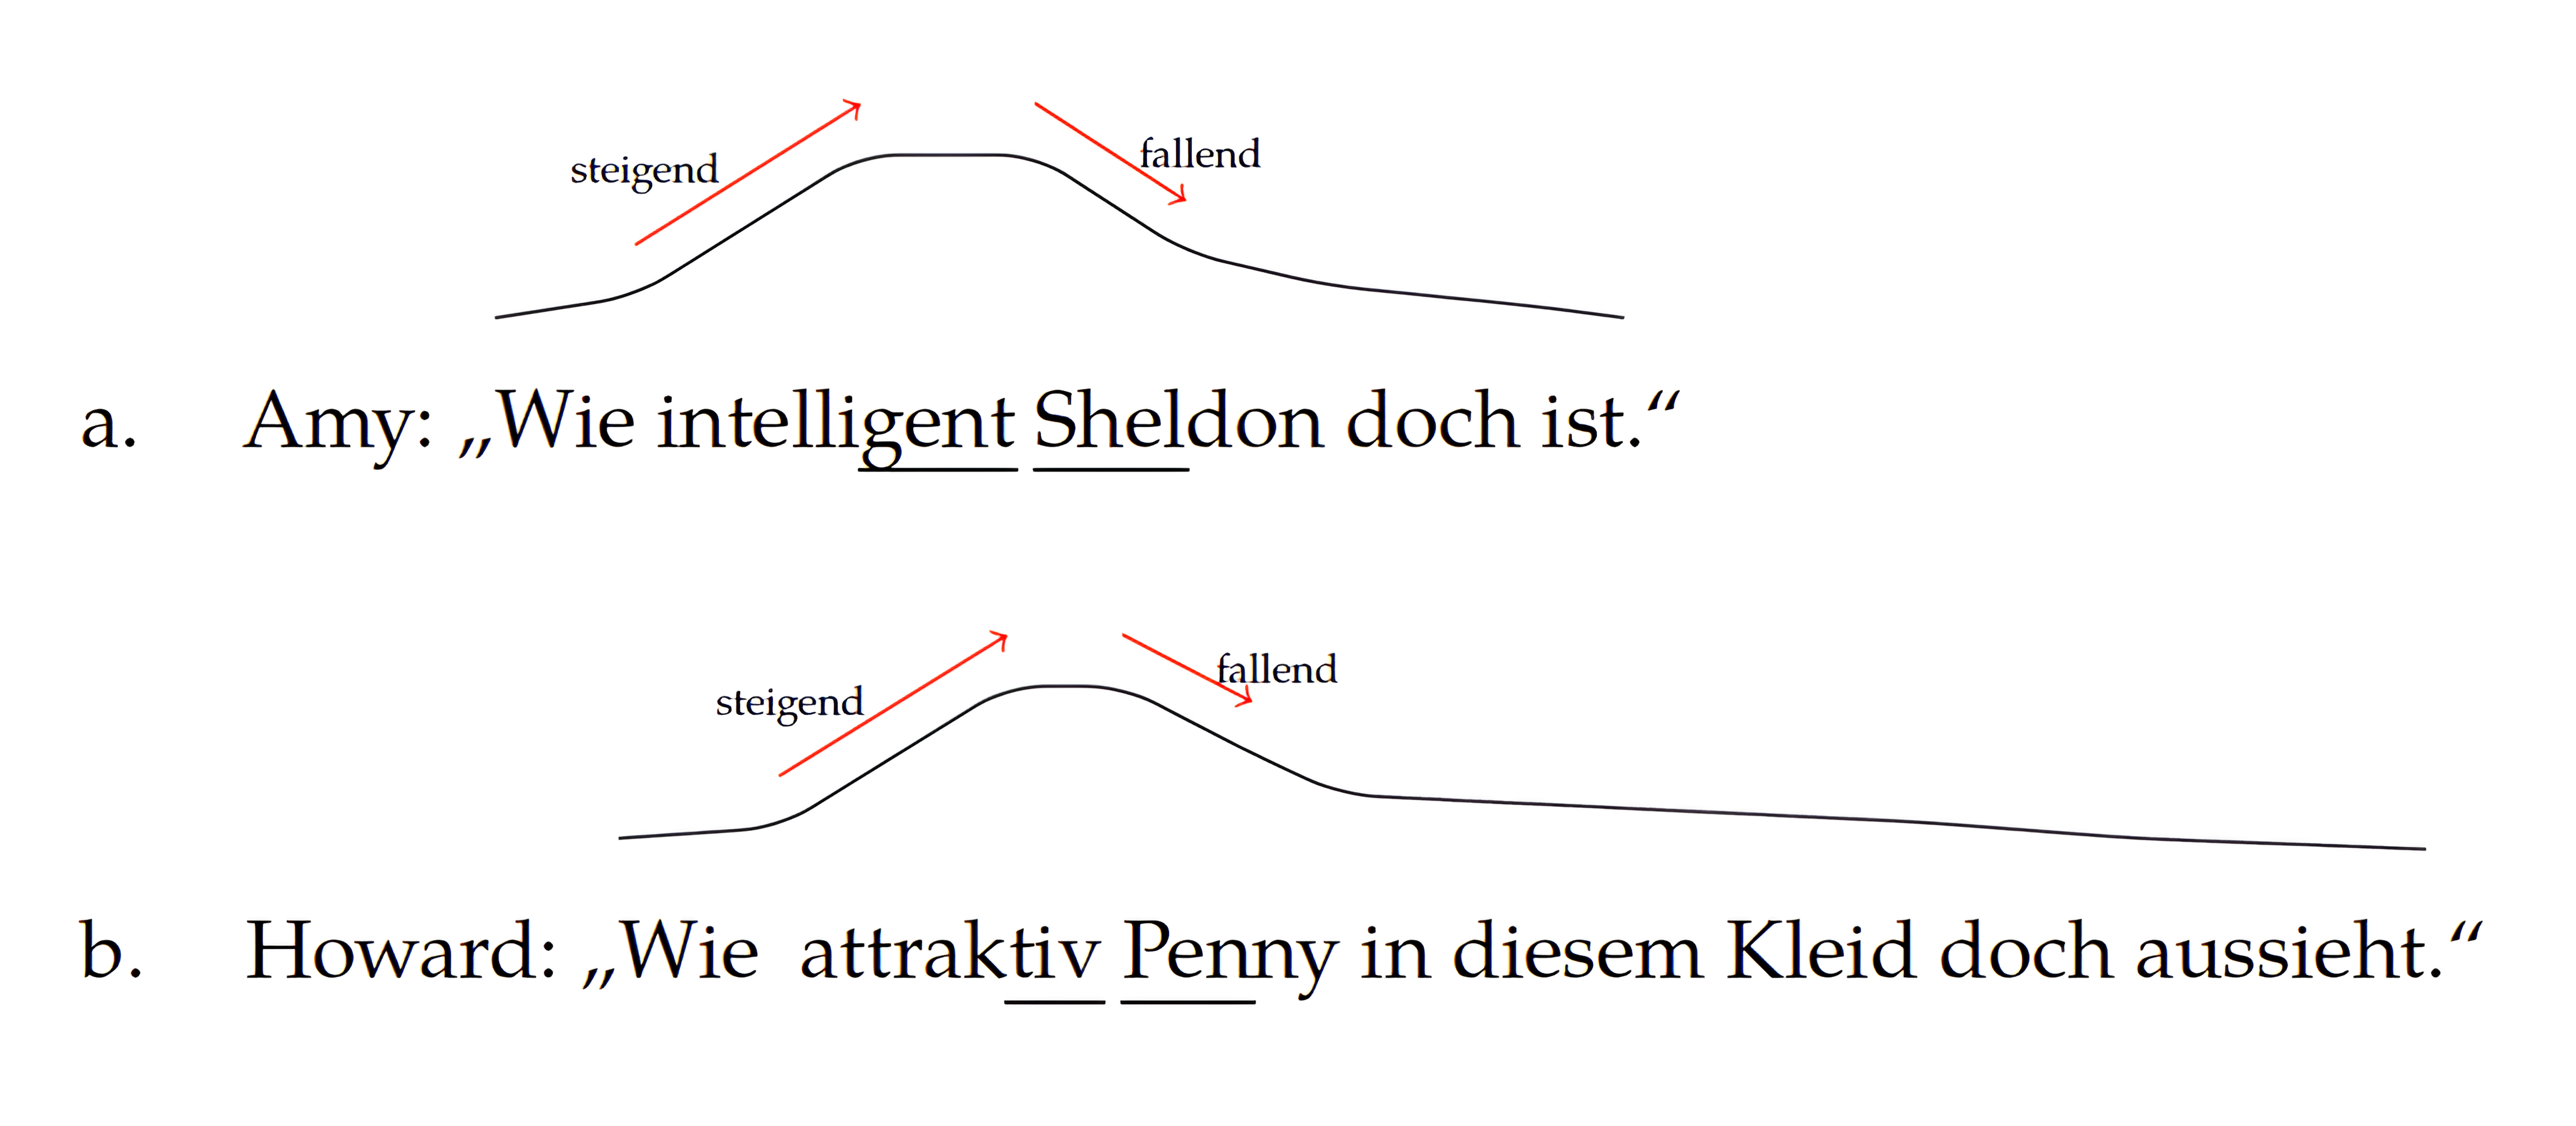
\includegraphics[width=0.9375\textwidth]{figures/Kontur3.png}%
  }
  \caption[Intonationskonturen für Exklamativsätze]
  {Intonationskonturen für die Sätze in Beispiel \REF{exklamativ}.}
  \label{Kont}
\end{figure}


\noindent Beispiel \REF{exklamativ} verdeutlicht, dass über den Exklamativsatz hinaus aus pragmatischer Sicht nichts weiter gesagt werden muss, um die Bewunderung Amys für Sheldons Intelligenz bzw. das Begehren Howards Penny gegenüber vollumfänglich und unmissverständlich zum Ausdruck zu bringen. Semantisch drücken die graduierbaren Adjektive \textit{intelligent} und \textit{attraktiv} einen überdurchschnittlich hohen Grad der im Satz beschriebenen Eigenschaft aus, der die Erwartungen des Sprechers potenziell übersteigt {\citep[vgl.][412]{Rett.2011}}. Durch die exklamative Konstruktion wird die durch den Kontext saliente Merkmalsausprägung in besonderem Maße herausgestellt, ohne dass ein Rückgriff auf eine vorherige Äußerung erforderlich ist. Ebenso wie Interjektionen haben Exklamativsätze ausschließlich expressive Bedeutung, die unabhängig von den Wahrheitsbedingungen des Satzes und deren Relevanz somit pragmatischer Natur ist (vgl. {\citealt[79]{Auer.2016}}).

\subsubsubsection{Expressive Adjektive}

Eine weitere Erscheinungsform stellen expressive Adjektive wie \textit{verdammt} oder \textit{verflucht} dar.\footnote{Das am häufigsten untersuchte expressive Adjektiv ist zweifelsohne \textit{damn}, das in der Literatur breiten Anklang gefunden und mitunter zur Diskussion von Expressivität angeregt hat (vgl. u.\,a. \citealt[]{Potts.2005, Potts.2007a, Potts.2007b}).} Diese können sowohl prädikativ als auch attributiv verwendet werden, wie die folgenden Beispiele zeigen:

 \ea  \label{ExAd1}
 \ea Penny: \glqq{}Ich finde Physik \textbf{öde}.\grqq{} \label{penn}
 \ex Bernadette: \glqq{}Dieses Kleid sieht \textbf{fantastisch} aus.\grqq{} \label{bernadette1}
  \z
 \z

  \ea  \label{ExAd10}
 \ea Kripke: \glqq{}Dieser \textbf{verdammte} Sheldon hat den Nobelpreis nicht verdient!\grqq{} \label{kripke2}
 \ex Sheldon: \glqq{}Dieser \textbf{verfluchte} Leonard hat wieder gegen die Mitbewohnervereinbarung verstoßen!\grqq{} \label{sheld}
 \z
 \z
Bei den beiden Sätzen in Beispiel \REF{ExAd1} handelt es sich der syntaktischen Form nach um Prädikative. Wenn Penny die Physik in Satz \REF{penn} als \textit{öde} bezeichnet, bezweckt sie damit keine qualitative Einordnung der wissenschaftlichen Disziplin, sondern sie möchte in erster Linie ihre persönliche Einstellung kundtun, indem sie ihr einen bestimmten (hier: niedrigen) Interessantheitsgrad zuschreibt. Ähnlich verhält es sich bei Bernadettes Äußerung in {Satz \REF{bernadette1}}: Auch hier drückt die Sprecherin ihre subjektive Bewertung aus und schreibt dem im Kontext bezeichneten Kleid (im Vergleich zu einem normal schönen Kleid) einen übermäßig hohen Ästhetikgrad zu. Während ebensolche Prädikative obligatorisch für die Bildung eines grammatischen Satzes sind und somit gemischte Bedeutungsbestandteile aufweisen, sind die attributiven Adjektive in den Sätzen \REF{kripke2} und \REF{sheld} hingegen als rein expressiv zu klassifizieren. Im Gegensatz zu ersteren leisten sie keinen Beitrag zum deskriptiven Gehalt der Äußerung und dienen daher ausschließlich der Einstellungsbekundung des Sprechers. Die attributiven Adjektive \textit{verdammte} und \textit{verfluchte} beschreiben also keine objektiven Merkmale von Sheldon oder Leonard, die als Unterscheidungskriterium zu anderen gleichnamigen Personen dienen. Stattdessen geben sie eine sprecherbezogene Charakterisierung der bezeichneten Person wieder, die grundsätzlich fakultativ ist und weggelassen werden kann, wenn der Sprecher seine persönliche Haltung zu Sheldon oder Leonard nicht ausdrücken will (vgl. \citealt[18]{Potts.2005}; {\citealt[131]{Gutzmann.2011}}).

Davon abzugrenzen sind die von \citet[]{Gutzmann.2013a} als \glqq{}functional mixed expressives\grqq{} bezeichneten attributiven Adjektive, die genauso wie die oben beschriebenen Prädikative gleichermaßen deskriptive und expressive Bedeutung tragen. Dies wird an den folgenden Sätzen illustriert:

\ea  \label{ExAd1b}
  \ea Penny: \glqq{}Ich laufe gerade von einem \textbf{beknackten} Vorsprechen zum nächsten -- ohne Erfolg.\grqq{} \label{penn1}
   \ex Amy: \glqq{}Sheldons \textbf{beschissene} Laune geht mir inzwischen schrecklich auf die Nerven.\grqq{} \label{amy1b}
 \z
 \z
Anders als bei den Adjektiven in Beispiel \REF{ExAd10} handelt es sich in \REF{ExAd1b} um Ausdrücke mit gemischten Bedeutungsanteilen: Neben der Sachverhaltsbeschreibung wird in beiden Fällen die Einstellung der Sprecherin ausgedrückt, die über den deskriptiven Gehalt der Äußerung hinausgeht. Dies erklärt {\citet[84f.]{Gutzmann.2019a}} damit, dass solche Qualitätsadjektive wie die exemplarisch in \REF{ExAd1b} herausgegriffenen gemäß ihres Ausprägungsgrades auf eine Skala abgebildet werden können: in Satz \REF{penn1} ausgehend von einem herausragenden Vorsprechen bis hin zu einem lausigen Vorsprechen, in Satz \REF{amy1b} von guter Laune bis hin zu miserabler Laune (vice versa). Ausschlaggebend für die Interpretation ist der Äußerungskontext, der die Merkmalsausprägung in die jeweils einschlägige Richtung steuert {\citep[vgl.][85]{Gutzmann.2019a}}.

Zweifelsfälle evaluativer Adjektive stellen die in der Literatur vielfach erörterten Prädikate dar, die mit individuellen Perzeptions- bzw. Geschmacksurteilen einhergehen (\glqq{}predicates of personal taste\grqq{} ({\citealt[]{Lasersohn.2005}})).

\ea  \label{ExAd2}
\ea Sheldon: \glqq{}Penny, die Spaghetti mit Würstchen sind \textbf{lecker}.\grqq{} \\
Leonard: \glqq{}Nein, sind sie nicht -- sie sind widerlich.\grqq{}
\ex Penny: \glqq{}Ich finde, dieses Nichtnewtonsche Fluid sieht \textbf{ekelhaft} aus.\grqq{} \\
Rajesh: \glqq{}Nein, gar nicht wahr. Es sieht total abgefahren aus.\grqq{}
 \z
 \z
Die Besonderheit solcher Adjektive wie die in \REF{ExAd2} aufgeführten ist, dass sie eine Eigenschaft beschreiben, die qua Semantik notwendigerweise sprecherbezogen und folglich nicht wahrheitsfunktional ist. Diese Subjektivität macht es jedoch schwierig, eine trennscharfe Grenze zwischen deskriptiver und expressiver Bedeutung zu ziehen, da es nicht möglich ist, die Aussage von Penny bzw. Sheldon als wahr oder falsch zu klassifizieren: Nur weil Sheldon die Spaghetti mit Würstchen lecker findet, heißt das nicht zwangsläufig, dass sie auch ein anderer mögen würde (vgl. die Antwort Leonards). Somit können in Abhängigkeit von Sprecher, Kontext und Perspektive verschiedene Aussagen und Qualitätsurteile zutreffen. In solchen Fällen wird der Wahrheitsgehalt der Äußerung also auf ein bestimmtes Subjekt relativiert, wobei sich der Geschmack eines Individuums von dem von anderen unterscheiden kann. Da es keinen objektiven Maßstab für solche Geschmacksurteile gibt, lässt sich bekanntlich nicht darüber streiten. Die Interpretation von Geschmacksprädikaten hänge primär davon ab, wer der kontextuelle \glqq{}Judge\grqq{} ({\citealt[665]{Lasersohn.2005}}), d.\,h. der Experiencer, ist, der oftmals, allerdings nicht notwendig dem Sprecher entspreche (vgl. \citealt[325f.]{Kaiser.2017b};; \citealt[224f.]{Kaiser.2017a}). Dadurch, dass sie die persönliche Meinung des Sprechers ausdrücken und demzufolge nicht bloß objektiv beschreibend sind, verfügen sie über Eigenschaften, die sie mit Expressiva teilen. Ob und inwiefern Geschmacksprädikate aufgrund der subjektiven Komponente tatsächlich als expressiv zu bewerten sind, wird in der Literatur kontrovers diskutiert (vgl. u.\,a. \citealt[]{Lasersohn.2005}; \citealt[]{Harris.2009}; \citealt[]{Gutzmann.2016a}).


\subsubsubsection{Expressive Nomen}

Abgesehen von expressiven Adjektiven stellen auch expressive Nomen, wie das von \citet[168]{Potts.2007b} ausführlich besprochene \textit{bastard}, eine Form von Expressivität dar. Diese kommen in der Regel in prädikativer oder appositiver Verwendung vor. Die Art des Gebrauchs bestimmt dabei den zugrunde liegenden Bedeutungstyp, wie die Beispiele \REF{ExNom} und \REF{ExNoma} illustrieren.

\ea  \label{ExNom}
\ea Amy: \glqq{}Sheldon ist ein \textbf{Genie}.\grqq{} \label{amy2}
\ex Leslie: \glqq{}Sheldon ist ein \textbf{Blödmann}.\grqq{} \label{leslie}
 \z
 \z

\ea  \label{ExNoma}
\ea Kripke: \glqq{}Dieser \textbf{Blödmann} Sheldon ist sogar verheiratet.\grqq{} \label{kripke4}
\ex Präsident Siebert: \glqq{}Dieses \textbf{Genie} Sheldon hat den Nobelpreis verdient.\grqq{} \label{siebert}
 \z
 \z
Während es sich in den Sätzen \REF{amy2} und \REF{leslie} um obligatorische expressive Nomen in prädikativer Verwendung handelt, sind die appositiv gebrauchten Nomen in den Sätzen \REF{kripke4} und \REF{siebert} optional. In Kopulakonstruktionen trägt die Bedeutung ebensolcher Nomen zur Proposition bei, weswegen sie als wahrheitsfunktional und somit deskriptiv zu klassifizieren sind. Demgegenüber weisen appositiv gebrauchte Nomen ausschließlich expressive Bedeutung auf, die keine Relevanz für den Wahrheitswert der Äußerung hat. Weil ihr Gebrauch in dieser Position fakultativ ist, können sie gleichfalls weggelassen werden, verbunden mit der Konsequenz, dass die subjektive Einstellungsbekundung des Sprechers verschwindet. Dies zeigt, dass den beiden Nomen \textit{Genie} und \textit{Blödmann} in Abhängigkeit der Verwendung unterschiedliche Bedeutungsanteile zukommen: Im Falle der prädikativen Verwendung erfolgt eine qualitative Beschreibung von Sheldon, d.\,h., Sheldon wird eine bestimmte Eigenschaft zugeschrieben (nämlich ein Genie oder ein Blödmann zu sein). Kommen die Nomen in Gestalt eines Appositivs daher, so drücken sie eine subjektive Bewertung des Sprechers aus, die ausschließlich expressiver Natur ist und nicht auf die Wahrheitsbedingungen einwirkt, wie u.\,a. \citet[270]{Gutzmann.2015a} erläutert. Eine besondere Form expressiver Nomen stellen die oftmals erörterten nationalitätsbezogenen, stereotypisierenden Beleidigungswörter wie \textit{Kartoffel} oder \textit{Kraut} (Ethnophaulismen für `Deutsche:r') (vgl. u.\,a. \citealt[2]{McCready.2010}; {\citealt[]{Croom.2013,Croom.2015}}; \citealt[20]{Gutzmann.2015a}; {\citealt[40]{Technau.2018}}) sowie emotional gefärbte Ausdrücke wie \textit{Gaul} oder \textit{Köter} mit gemischten Bedeutungstypen dar, die in Abschnitt \ref{Eigenschaften} genauer betrachtet werden.

\subsubsubsection{Modalpartikeln}

Auch Modalpartikeln wie \textit{doch} oder \textit{eben}, die häufig von polysemen Ausdrücken anderer Wortarten (z.\,B. Adverbien und Adjektiven) abgeleitet sind, werden in der Literatur als Ausprägungsform von Expressivität beschrieben. Wie {\citet[9]{Weydt.1969}} anmerkt, wurden Modalpartikeln früher häufig als funktionslose, weglassbare \glqq{}`Flick'- oder `Füllwörter'\grqq{} betrachtet, die vorwiegend in der gesprochenen {(Umgangs-)Sprache} zu finden und in der Schriftsprache zu vermeiden seien. Im Unterschied zu anderen Formen (bspw. Interjektionen) drückt der Sprecher seine Einstellung zum Geäußerten durch Modalpartikeln nicht direkt aus. So modifizieren sie nicht nur einen graduierbaren Ausdruck derselben Phrase, sondern den Satz als Ganzes {\citep[vgl.][603]{Duden.2016}}. Die Einstellungsspiegelung kann je nach verwendeter Partikel kommunikativ unterschiedlich wirken, z.\,B. permissiv oder provokativ: \textit{Komm \uline{ruhig} her} (beruhigend durch fehlenden Intensitätsgrad) vs. \textit{Komm \uline{bloß} her} (drohend aufgrund hohen Intensitätsgrades) (vgl. {\citealt[20f.]{Batinic.2015}}; {\citealt[24]{Pittner.2015}}). Daraus lässt sich schließen, dass Modalpartikeln entgegen früherer Behauptungen weder bedeutungslos noch frei austauschbar sind: \glqq{}Sie haben aber Bedeutungen. Jedoch vermitteln diese nicht Kerninformationen, sondern Zusatzinformationen\grqq{} (\citealt[89]{Weydt.1969}), die auf die subjektive Sprecherbewertung abzielen. Da sie allerdings keine eigene, mittels Wahrheitswerten beschreibbare lexikalische Bedeutung tragen und somit auch keine neuen Informationen zum deskriptiven Gehalt beisteuern,\footnote{Hiervon auszunehmen ist die von \citet[]{Zimmermann.2004} diskutierte Modalpartikel \textit{wohl}, die infolge ihrer epistemischen Interpretation durchaus relevant für die \mbox{Wahrheitsbedingungen sei}.} haben sie eine rein expressive Bedeutung und sind daher pragmatische Funktionsträger. Dies wird im Anschluss mithilfe der Modalpartikeln \textit{halt}, \textit{ja} und \textit{wohl} exemplifiziert.

\ea  \label{MoPa}
\ea Präsident Siebert: \glqq{}Sheldon ist \textbf{halt} anstrengend.\grqq{} \label{siebert2}
\ex Bernadette: \glqq{}Howard wohnt \textbf{ja} noch bei seiner Mutter.\grqq{} \label{bernadette2}
\ex Rajesh: \glqq{}Penny hat die Schauspielrolle \textbf{wohl} bekommen.\grqq{} \label{raj2}
 \z
 \z
Die Sätze im obigen Beispiel zeigen, dass die Sprechereinstellung in Abhängigkeit von der jeweils verwendeten Partikel verschieden ausgedrückt wird.\footnote{Zu erwähnen ist, dass Modalpartikeln grundsätzlich ambig sein können und deswegen stets kontextsensitiv bewertet werden müssen \citep[vgl.][603]{Duden.2016}.} Die Modalpartikel \textit{halt} in Satz \REF{siebert2} gibt an, dass Präsident Siebert die Unveränderlichkeit des Sachverhalts bekannt ist und er sich (notwendigerweise) damit abgefunden hat \citep[vgl.][10]{Abraham.1986}. Obendrein drückt Bernadette mit \textit{ja} in Satz \REF{bernadette2} aus, dass sie annimmt, der Umstand, dass Howard bei seiner Mutter wohnt, sei unkontrovers und Teil des gemeinsamen Wissenshintergrunds, den sie und der Adressat miteinander teilen (vgl. {\citealt[36f.]{Weydt.1969}}; {\citealt[19]{Abraham.1986}}). Durch die Modalpartikel \textit{wohl} in Satz \REF{raj2} erhält {Rajeshs} {Äußerung} eine epistemische Interpretation, mithilfe derer er seine bloße Vermutung hinsichtlich der Korrektheit der Sachlage mitteilt, ohne sich eindeutig darauf festlegen zu wollen \citep[vgl.][18]{Abraham.1986}.

Im Hinblick auf \textit{wohl} ist auch die sprachgeschichtliche Entwicklung interessant, die der Ausdruck auf dem Weg zur Modalpartikel durchlaufen hat. So schildert \citet[219f.]{Kip.1900}, dass sich das Adverb zunächst im Alt- und Mittelhochdeutschen\footnote{Das Althochdeutsche umfasst die Sprachstufe zwischen 750 und 1050, woran sich im Zeitraum von 1050 bis 1350 das Mittelhochdeutsche anschließt \citep[vgl.][5f.]{Nuebling.2013}.} zum Intensivierer mit der Bedeutung `völlig, gewiss, sehr' entwickelt hat. Diese Gradbedeutung hat sich mit der Zeit jedoch abgeschwächt, sodass die Partikel in neuerer Sprachperiode nur noch modal zum Ausdruck von Behauptungen oder Mutmaßungen gebraucht wird.

\subsubsubsection{Pronomen}

Ein weiterer, wenn auch weniger evidenter Fall von Expressivität liegt bei Ausdrücken mit sozialer Bedeutung wie Nähe- und Distanzformen vor, die in verschiedenen Sprachen zu finden sind (bspw. im Deutschen oder Französischen). Obwohl sie weder Einstellungsbekundungen noch emotionale Zustände des Sprechers wiedergeben, sind sie dennoch mit einer rein expressiven Funktion versehen, die nicht auf deskriptiver Ebene {verankert ist}.

\ea  \label{NäDi}
\ea Präsident Siebert: \glqq{}Ich rufe \textbf{Sie} an, Sheldon.\grqq{} \label{siebert3}
\ex Bernadette: \glqq{}Hast \textbf{du} Penny gesehen, Leonard?\grqq{} \label{bernadette3}
 \z
 \z
Anhand der Sätze in Beispiel \REF{NäDi} lässt sich verdeutlichen, dass es keinen Unterschied in der referentiellen Bedeutung der förmlichen Anrede \textit{Sie} und der formlosen Balanceform \textit{du} gibt. Nach \citet[33]{Loebner.2002} bedeutet dies, dass sich beide Anredeformen insofern nicht voneinander unterscheiden, als sie gleichermaßen auf einen bestimmten Adressaten Bezug nehmen. Somit referieren sowohl Präsident Siebert mit der Verwendung der Distanzform \textit{Sie} in Satz \REF{siebert3} als auch Bernadette mit der Näheform \textit{du} in Satz \REF{bernadette3} auf eine bestimmte Person, nämlich Sheldon und Leonard. Darüber hinaus geht \textit{Sie} zusätzlich mit einem sozialen Bedeutungsanteil einher, der der informellen Form gänzlich fehlt \citep[vgl.][33]{Loebner.2002}. Dieser nicht-propositionale Bedeutungsbestandteil ermöglicht es dem Sprecher, per Konvention eine interpersonelle Distanz zum Gegenüber anzuzeigen, die in der Regel auf Unbekanntheit, Höflichkeitsstreben oder eine soziale Hierarchie zurückgeht \citep[vgl.][18]{Pafel.2016}. Infolgedessen ist anzunehmen, dass der Unterschied zwischen dem formlosen \textit{du} und dem förmlichen \textit{Sie} durch einen Kontrast in der sozial-expressiven Komponente bedingt ist. Nach {\citet[26]{Gutzmann.2019a}} handelt es sich bei solchen Pronomen um gemischte Expressiva, die zugleich deskriptive wie expressive Bedeutungsbestandteile aufweisen. Seiner Notation folgend befindet sich auf der deskriptiven Ebene der Adressat, der den Referenten des jeweiligen Kontexts darstellt. Auf der expressiven Ebene sieht er die für die Gebrauchsbedingungen relevante Unterscheidung zwischen der formellen und informellen Form verankert: \glqq{}[C]hoosing the wrong pronoun can never make an otherwise true sentence false, but it may result in a high degree of social infelicity.\grqq{} (\citealt[26]{Gutzmann.2019a}). Fehlt diese expressive Zusatzkomponente, so kann der Ausdruck im Kontext folglich als unpassend oder gar unhöflich aufgefasst werden: Auch wenn Präsident Siebert Sheldon gegenüber im Prinzip ebenso das weniger formelle \textit{du} verwenden könnte, würde es aufgrund der sozialen  Hierarchie der Arbeitgeber-Arbeitnehmer-Beziehung möglicherweise als unangemessen wahrgenommen. Genauso inadäquat kann ihr Vorhandensein in informellen Kontexten sein. So riefe es bei Leonard vermutlich starke Irritation hervor, wenn ihn Bernadette trotz jahrelanger Freundschaft plötzlich siezte, da eine solche förmliche Ausdrucksweise in dem Fall nicht angebracht ist.

\subsubsubsection{Dativus ethicus}

Daneben sind auch ethische Dative im Allgemeinen eng mit dem Begriff der Expressivität verbunden, die bspw. in verschiedenen germanischen, romanischen oder slawischen Sprachen vorkommen und nach \citet[61]{Wegener.1989} als \glqq{}Ausdruck familiärer Vertrautheit\grqq{} gelten. Dies zeigt \citet[26f.]{Gutzmann.2019a} am Beispiel des Englischen und Deutschen wie folgt:

\ea  \label{EtDat}
\ea I want \textbf{me} an iPod. \hfill  \citep[][175]{Horn.2008} \label{iPod}
\ex Dass du \textbf{mir} ja nicht zu spät kommst. \hfill  \citep[][5]{Lambert.2007} \label{spät}
 \z
 \z
In beiden Sätzen \REF{iPod} und \REF{spät} drückt der freie Dativ eine emotionale Beteiligung des Sprechers in Form einer Bitte oder einer Warnung aus, die nicht Teil des deskriptiven Gehalts der Äußerung ist. Dementsprechend hat er keinerlei Auswirkungen auf die Wahrheitsbedingungen des Satzes. Stattdessen ist der ethische Dativ vielmehr als zusätzliche Bedeutungskomponente zu klassifizieren, mit deren Hilfe der Sprecher seine persönliche Involviertheit in den Sachverhalt anzeigen kann \citep[vgl.][27]{Gutzmann.2019a}. \glqq{}[D]ie Quelle der ausgedrückten Einstellung\grqq{} (\citealt[68]{Wegener.1989}) liege dabei stets beim Sprecher, was im obigen Beispiel durch das Reflexivpronomen der 1. Person \textit{mir} (bzw. \textit{me}) ausgedrückt wird. Da das jeweilige Pronomen keinen Einfluss auf den deskriptiven Gehalt nimmt, kann es ohne Bedeutungsänderung eliminiert werden. Die unmittelbare Folge des Auslassens ist allerdings, dass die expressive Bedeutungskomponente, d.\,h. die ausgedrückte Sprecherbeteiligung, verschwindet und nur der deskriptive Gehalt der Äußerung bestehen bleibt. Laut \citet[69]{Wegener.1989} dient der ethische Dativ somit vordergründig dazu, \glqq{}auf das emotiv-affektive Involviertsein des Sprechers zu verweisen bzw. ein solches Involviertsein beim Hörer {zu unterstellen\grqq{}}.

\subsubsubsection{Expressive Vokative}

Auch \glqq{}expressive Vokative\grqq{} (\citealt[172]{Gutzmann.2019a}) werden in der theoretischen Literatur als eine Ausprägung von Expressivität behandelt. Während klassische Vokative normalerweise durch Substantive oder Eigennamen repräsentiert und nach \citet[787]{Zwicky.1974} aus pragmatischer Sicht hauptsächlich zur Aufmerksamkeitssteuerung verwendet werden, bestehen expressive Vokative aus einem Personalpronomen und einem (expressiven) Nomen. Dies macht \citet[188]{Gutzmann.2019a} an den folgenden Beispielen deutlich:

\ea  \label{ExVo}
\ea \textbf{You idiot!} \label{idiot}
\ex \textbf{You bastard!} \label{bastard0}
 \z
 \z

\ea  \label{ExVo2}
\ea \textbf{You linguist!} \label{linguist}
\ex \textbf{You philosopher!} \label{philosopher}
 \z
 \z
Die beiden Sätze in Beispiel \REF{ExVo} beinhalten mit \textit{idiot} und \textit{bastard} expressive Nomen, die qua Semantik eine bewertende, in diesem Fall negative Sprechereinstellung ausdrücken. Dagegen handelt es sich bei \textit{linguist} und \textit{philosopher} {in Beispiel \REF{ExVo2}} um neutrale Nomen, die über ihre lexikalische Bedeutung hinaus keine zusätzliche evaluative Bedeutungskomponente aufweisen. Dennoch erhalten die Ausdrücke durch solche Vokativkonstruktionen eine expressive Interpretation, die als eine persönliche Bewertung des Sprechers aufzufassen ist. Der Unterschied zwischen dem ersten und zweiten Satzpaar liegt im Wesentlichen darin, dass die Sprechereinstellung bei ersterem aufgrund der klar wahrnehmbaren evaluativen Semantik der Ausdrücke erheblich stärker kommuniziert wird. Bei letzterem wird die Sprechereinstellung hingegen erst durch die Konstruktion ausgedrückt, wodurch sie als vergleichsweise moderater und weniger offensiv wahrgenommen wird (vgl. {\citealt[212]{dAvis.2013}}; {\citealt[188f.]{Gutzmann.2019a}}). In Abhängigkeit des Kontexts können ebensolche eigentlich neutralen Nomen wie \textit{linguist} und \textit{philosopher} in Vokativkonstruktionen gleichermaßen positiv wie auch negativ interpretiert werden, d.\,h. als Ausdruck der Bewunderung oder als Beschimpfung. Gegenläufig zu den klassischen Vokativen haben expressive Vokative keine aufmerksamkeitssteuernde Funktion. Aus diesem Grund ist es mit ihnen nicht möglich, zwischen einer Masse an Referenten und Einzelpersonen zu differenzieren, weswegen sie \citet[]{dAvis.2013} als \glqq{}pseudo-vocative constructions\grqq{} bezeichnen {\citep[vgl.][189]{Gutzmann.2019a}}.

\subsubsection{Eigenschaften von Expressivität}  \label{Eigenschaften}
Gegenstand dieses Abschnitts sind die Merkmale von sprachlicher Expressivität sowie die Kriterien, die in der theoretischen Literatur für die Unterscheidung zwischen deskriptivem und expressivem Gehalt angeführt werden. Aus der Akzeptanz zweier Bedeutungstypen und der Definition von Expressivität ex negativo ergeben sich mehrere Streitfragen: Worin besteht der semantische Unterschied zwischen deskriptiver und expressiver Bedeutung? Wie lassen sich die Bedeutungstypen voneinander abgrenzen? Und was sind die Besonderheiten expressiver Bedeutung? 
Einige Autor:innen, (z.\,B. {\citealt[]{Cruse.1986}}, {\citealt[]{Kaplan.1997}} oder {\citealt[]{Potts.2005, Potts.2007a}}), haben sich aus formal-semantischer Perspektive mit den Eigenschaften von Expressivität auseinandergesetzt. Als wegbereitend gelten auf diesem Gebiet vor allem die Ausführungen von {\citet[]{Potts.2007a}}. Er baut im Kern auf den in Abschnitt {\REF{Arbeitsdefinition}} geschilderten Ansätzen auf und entwickelt durch die Annahme von zwei verschiedenen Dimensionen einen neuen Zugang zu sprachlicher Bedeutung. In diesem Kontext erarbeitet er sechs Kriterien, die es ermöglichen, expressive Bedeutung als solche zu identifizieren und von deskriptiver zu separieren. Diese Kriterien werden im Anschluss präsentiert.

Das erste Kriterium nennt \citet[167ff.]{Potts.2007a} \textit{Independence} (`Unabhängigkeit'). Nach diesem stellen die beiden Bedeutungstypen zwei separate, voneinander unabhängige Dimensionen dar. Da die expressive Ebene nicht an die deskriptive Ebene gebunden sei, können Sprecher die in einer Äußerung enthaltenen expressiven Bedeutungsbestandteile beliebig verändern oder weglassen, ohne dass dies auf den deskriptiven Gehalt einwirke. Dieses {Prinzip} lässt sich im Sinne von \citet[168]{Potts.2007a} und \citet[9]{dAvis.2019b} wie folgt illustrieren:

\ea  Dieser \,\textbf{bescheuerte}\,/\,\textbf{dämliche} Sheldon ist ein Nerd. \label{sheldon}
\ea deskriptiv: Sheldon ist ein Nerd.
\ex expressiv: Der Sprecher mag Sheldon nicht.
 \z
 \z

Beispiel \REF{sheldon} demonstriert, dass eine Variation derjenigen Ausdrücke, die expressive Bedeutung aufweisen (d.\,h. \textit{bescheuerte} oder \textit{dämliche}) keine Veränderung des deskriptiven Gehalts nach sich zieht: Er bleibt von der Änderung auf expressiver Ebene unangetastet. Gleichsam kann das expressive Adjektiv eliminiert werden, ohne dass die Proposition davon betroffen ist. Dies zeigt, dass es sich bei deskriptiver und expressiver Bedeutung um zwei eigenständige, voneinander getrennte Ebenen handelt, deren Einzelbedeutungen zur Gesamtbedeutung des Satzes verknüpft werden. Aufgrund ihrer Expressivität haben die verwendeten attributiven Adjektive keinen Einfluss auf die Wahrheit oder Falschheit des Satzes. Stattdessen drücken sie die persönliche Einstellung des Sprechers aus, bei der statt Wahrheitsbedingungen die oben beschriebenen Gebrauchsbedingungen Anwendung finden. Gemäß der in {\citet[5]{Gutzmann.2013a}} vorgeschlagenen Notation lassen sich die beiden semantischen Dimensionen von Beispiel \REF{sheldon} folgendermaßen schematisch darstellen:\footnote{Zu beachten ist, dass die Konklusion der deskriptiven Bedeutung des Satzes entspricht, während die Prämisse die expressive Bedeutung in Form einer Zusatzebene repräsentiert.} \medskip

Dieser bescheuerte Sheldon ist ein Nerd = \begin{large} $\frac{\text{Der Sprecher mag Sheldon nicht}}{\text{Sheldon ist ein Nerd}}$ \end{large} \medskip

\citet[8]{Kaplan.1997} zufolge kann expressive Bedeutung weder negiert noch konditionalisiert werden: Wenn der Adressat dem Sprecher beim obigen Satz widerspricht, weist er zwar das Zutreffen des bezeichneten Sachverhalts zurück, nicht aber den zusätzlichen expressiven Gehalt. Dies sei ein weiterer Indikator für die Eigenständigkeit der Bedeutungsdimensionen.

Dessen ungeachtet weicht \citet[168]{Potts.2007a} das Unabhängigkeitskriterium auf und ergänzt, dass die beiden Bedeutungstypen allerdings nicht völlig unabhängig voneinander sind, greifen expressive Ausdrücke doch insofern auf die deskriptive Ebene zu, als sie darauf ihr Argument finden. So benötigt das aus semantischer Sicht als Prädikat zu betrachtende \textit{bescheuerte} oder \textit{dämliche} ein Argument, auf dem es operiert. Ebendieses findet es im deskriptiven Gehalt, genauer gesagt im Eigennamen, d.\,h. in \textit{Sheldon}, wie \citet[9]{dAvis.2019b} erläutern. Inwiefern die Bedeutungstypen einander noch bedingen, wird beim vierten Kriterium wieder aufgegriffen.

Das zweite Kriterium bezeichnet \citet[169ff.]{Potts.2007a} als \textit{Nondisplaceability} (`Nicht-Verschiebbarkeit'). Dieses resultiert aus dem deiktischen Verhalten von Expressiva, demgemäß sich expressive Bedeutung unmittelbar auf die Parameter der Äußerungssituation, d.\,h. Sprecher, Ort und Zeit etc., bezieht: \glqq{}Expressives cannot (outside of direct quotation) be used to report on past events, attitudes, or emotions, nor can they express mere possibilities, conjectures, or suppositions.\grqq{} ({\citealt[169]{Potts.2007a}}). Diese Beobachtung kongruiert mit dem von {\citet[8]{Kaplan.1997}} beschriebenen Projektionsverhalten. In der Folge vergleicht {\citet[272]{Cruse.1986}} die unmittelbare Wirkung von expressiven Ausdrücken bspw. mit Gesichtsausdrücken wie Lächeln oder Stirnrunzeln sowie anderen sprecherorientierten Gesten, die ebenfalls nur zum Zeitpunkt der Äußerung angebracht sind. Die Idee dahinter wird in Anlehnung an die von {\citet[10]{dAvis.2019b}} formulierten Beispielsätze verdeutlicht.\footnote{Die Raute (\#) symbolisiert hier und im weiteren Verlauf, dass der Satz bzw. eine solche Fortsetzung pragmatisch nicht im intendierten Sinne möglich ist.}

\ea   \label{sheldon2}
\ea[]{Dieser Klugscheißer Sheldon ist nicht überheblich. (\#Ich kann ihn gut leiden.) \label{negation1}}
\ex[]{Glücklicherweise ist es nicht wahr, dass dieser Klugscheißer Sheldon überheblich ist. (\#Ich kann ihn gut leiden.) \label{negation2}}
\ex[\#]{Wenn dieser Klugscheißer Sheldon ein netter Mensch ist, sollte er aufgrund seiner Überheblichkeit keine Frau finden. \label{konditional}}
\ex[]{Es ist möglich, dass sich dieser Klugscheißer Sheldon wieder überheblich benehmen wird. (\#Andererseits ist er vielleicht gar kein Klugscheißer.) \label{moeglichkeit}}
\ex[]{Dieser Klugscheißer Sheldon hat sich gestern überheblich benommen. (\#Aber heute ist er kein Klugscheißer, weil er sich normal benimmt.) \label{tempus}}
 \z
 \z

Nach Erklärung von {\citet[10]{dAvis.2019b}} werden die mit einer Raute ausgestatteten Interpretationen aus verschiedenen Gründen blockiert: Während sich die Negation in \REF{negation1} und \REF{negation2} nicht auf die persönliche Einstellung des Sprechers gegenüber Sheldon bezieht, sondern alleine die ihm zugeschriebene Charaktereigenschaft und somit den deskriptiven Gehalt negiert, wird {Satz \REF{konditional}} dadurch verhindert, dass das expressive Nomen \textit{Klugscheißer} nicht konditionalisiert werden kann. Ebenso wenig kann es von einem Möglichkeitsoperator erfasst werden, wodurch eine Interpretation wie die in \REF{moeglichkeit} ausgeschlossen ist. Zudem kann der Ausdruck in {Satz \REF{tempus}} nicht temporal modifiziert werden \citep[vgl.][10]{dAvis.2019b}. Daran ist zu erkennen, dass die Einstellungsbekundung des Sprechers durch die Verwendung des expressiven Nomens \textit{Klugscheißer} in allen Fällen erhalten bleibt und es nicht möglich ist, diese z.\,B. durch einen beschwichtigenden Zusatz aufzuheben. In diesem Kontext verweist \citet[15]{Gutzmann.2019a} auf die Ähnlichkeit zwischen expressiver Bedeutung und Präsuppositionen, projizieren doch beide gleichermaßen auf die Äußerung als Ganzes.

Das dritte Kriterium, das \citet[173ff.]{Potts.2007a} definiert, nennt sich \textit{Perspective dependence} (`Perspektivenabhängigkeit'). Dieses besagt, dass expressive Bedeutung grundsätzlich subjektive Einstellungen, Evaluationen und Emotionen ausdrückt, die sich auf eine bestimmte Perspektive beziehen. Dies sei im Regelfall der Sprecher, der als Experiencer einen Sachverhalt von seinem Standpunkt aus beurteile und seine Haltung entsprechend zum Ausdruck bringe. Eine Ausnahme stelle jedoch Redewiedergabe dar, bei der ein Perspektivenwechsel erfolgen könne, der dazu führe, dass eine andere, im Kontext saliente Person der Einstellungsträger ist \citep[vgl.][175]{Potts.2007a}. Dies zeigt das in der Literatur oft herangezogene Beispiel von {\citet[6]{Kratzer.1999}}:

\ea  My father screamed that he would never allow \uline{me} to marry \uline{that bastard Webster}. \label{bastard}
\z

In \REF{bastard} kommt aufgrund des darin enthaltenen Verbum dicendi keine andere Interpretation infrage, als dass der expressive Bedeutungsanteil dem Wortlaut des Vaters entspricht. Die Einstellungsspiegelung erfolgt also nicht in der Äußerungssituation, sondern zu einem vorangegangenen Zeitpunkt, auf den hier Bezug genommen wird \citep[vgl.][6]{Kratzer.1999}. Dass der Vater in diesem Fall der Einstellungsträger ist, hat nach \citet[11]{dAvis.2019b} neben dem erwähnten Verb des Sagens auch psychische Realität: So beabsichtige der Sprecher wohl kaum jemanden zu heiraten, der seiner Ansicht nach ein schlechter Mensch ist. Ergänzend demonstrieren sie, dass es durch eine Variation des Kontexts möglich ist, die verbalisierte Einstellung nicht dem Subjekt des übergeordneten Satzes, sondern dem Sprecher zuzuschreiben:

\ea  Mein Vater sagte, dass er es mir nie erlauben würde, dieses Arschloch Webster umzubringen.
\z

\citet[173]{Potts.2007a} erklärt den Perspektivenwechsel mit dem auf {\citet[]{Lasersohn.2005}} zurückgehenden kontextuellen \glqq{}Judge\grqq{}, d.\,h. dem Richter, der in einer Situation ein Urteil fälle und für gewöhnlich dem Sprecher entspreche. In Abhängigkeit des Kontexts bestehe die Möglichkeit, dass die Richterrolle von jemand anderem als dem Sprecher eingenommen werde. Dies ist abgesehen vom obigen Beispiel \REF{bastard} u.\,a. bei den in der Literatur vielfach diskutierten Geschmacksprädikaten festzustellen (vgl. bspw. {\citealt[]{Lasersohn.2005}}; \citealt[]{Harris.2009}; \citealt[]{Gutzmann.2016a}; {\citealt[]{Kaiser.2017b, Kaiser.2017a}}).

Das vierte Kriterium, das \citet[176ff.]{Potts.2007a} anführt, nennt sich \textit{Descriptive ineffability} (`Nicht-Beschreibbarkeit'). Dahinter steckt die bereits von {\citet[156]{Hayner.1956}} thematisierte Beobachtung, dass sich die Bedeutung von expressiven Ausdrücken nicht oder nicht hinreichend deskriptiv umschreiben lässt. Aufgrund des Umstands, dass nicht-expressive, assertive Paraphrasen nicht die gewünschte Ausdrucksstärke in sich tragen, seien sie für den Sprecher in der Äußerungssituation wenig zufriedenstellend. Laut \citet[12]{dAvis.2019b} fällt es Sprechern ohnehin schwer, expressive Bedeutungsbestandteile deskriptiv zu paraphrasieren: Versuche man bspw., einen expressiven Ausdruck wie \textit{Klugscheißer} in ein deskriptives Äquivalent zu überführen, so gehe die für Expressiva charakteristische Zusatzkomponente, die Einstellungsspiegelung also, verloren. So bedeute \glqq{}[d]ie Verwendung von \textit{Drecksack} in Bezug auf eine bestimmte Person \textelp{} nicht einfach, dass diese Person ein schlechter Mensch ist.\grqq{} ({\citealt[12]{dAvis.2019b}}). Stattdessen werde zusätzlich zum deskriptiven Gehalt ebenso die evaluative, in dem Fall negative Einstellung des Sprechers mit kommuniziert, die der deskriptiven Paraphrasierung gänzlich fehle. Aus diesem Grund lässt sich die Bedeutung eines expressiven Ausdrucks nach Auffassung von {\citet[10]{Kaplan.1997}} am ehesten durch seine korrekte Verwendung im Kontext beschreiben.

Auch Potts' (2007: 179ff.) fünftes Kriterium, \textit{Immediacy} (`{Unmittelbarkeit}'), wurde schon von \citet[151]{Hayner.1956} und \citet[285]{Cruse.1986} erkannt. Nach diesem verhalten sich expressive Ausdrücke infolge ihrer zielgerichteten, kraftvollen Natur wie performative Sprechakte\footnote{Genau wie Expressiva unterliegen auch Performativa nicht den Wahrheitsbedingungen, sondern vielmehr den Glückens- bzw. Angemessenheitsbedingungen
der fraglichen Situation (vgl. u.\,a. \citealt[75f.]{Austin.1972};; \citealt[176f.]{Chierchia.1990}).} und müssen bloß geäußert werden, um den intendierten Effekt zu erlangen: \glqq{}Like {performatives}, the act of uttering an expressive morpheme is sufficient for conveying its content. \textelp{} [T]he act of uttering an expressive \textit{is} the emotive performance.\grqq{} ({\citealt[180]{Potts.2007a}}). Dies lässt sich angelehnt an {\citet[12]{dAvis.2019b}} unter Zuhilfenahme des obigen {Beispiels \REF{tempus} aufzeigen}:

\ea  Dieser Klugscheißer Sheldon hat sich gestern überheblich benommen. (\#Aber heute ist er kein Klugscheißer, weil er sich normal benimmt.)
\z

Die Äußerung des expressiven Ausdrucks \textit{Klugscheißer} im genannten Beispiel bewirkt eine Veränderung des Kontexts, in deren Folge es für den Sprecher nicht mehr möglich ist, die damit einhergehende negative Einstellung {zurückzunehmen} oder zu relativieren. Mit anderen Worten: \glqq{}Das, was ein Sprecher damit ausdrücken will, ist im Diskurs nicht verhandelbar.\grqq{} (\citealt[12]{dAvis.2019b}). Dies lässt sich auch mittels Frage und Negation überprüfen, wie ein von \citet[31]{Gutzmann.2015a} übernommenes Beispiel illustriert:

\ea   Descartes was not a Kraut. \#But I like Germans. \label{gutzi} \\
	A: Was Descartes a Kraut? \\
    B: \#No, Germans are nice.
\z

Wie zuvor kann die bereits geäußerte negative Einstellung auch in dem \REF{gutzi} aufgeführten Beispiel nicht neutralisiert werden. Dies erklärt {\citet[31]{Gutzmann.2015a}} damit, dass Frage und Negation ausschließlich auf die wahrheitsfunktionale Ebene einwirken. Die expressive, gebrauchskonditionale Ebene bleibe davon jedoch unberührt, wie er anhand der beiden voneinander unabhängigen Bedeutungsdimensionen folgendermaßen präzisiert: \medskip

Descartes was not a Kraut. = \begin{large} $\frac{\text{Kraut}}{\text{$\neg$(Descartes was a German)}}$ \end{large} \medskip

Was Descartes a Kraut? = \begin{large} $\frac{\text{Kraut}}{\text{?(Descartes was a German)}}$ \end{large} \medskip

\noindent \citet[12]{dAvis.2019b} ergänzen weiterhin, dass die Wahrheit der kommunizierten Sprechereinstellung vom Adressaten nicht angezweifelt werden kann, wie Beispiel \REF{pups} demonstriert.

\ea  \label{pups}
\ea Howard: \glqq{}Penny hat Leonard bezüglich ihres College-Abschlusses angelogen.\grqq{} \label{penny}
\ex	Rajesh: \glqq{}Nein, das ist nicht wahr.\grqq{} ($\rightarrow$ Sie hat ihn nicht angelogen.) \label{penny1}
\ex Rajesh: \glqq{}\#Nein, das hast du jetzt nicht assertiert.\grqq{} ($\nrightarrow$ Sie hat ihn nicht angelogen.)\label{penny2}
 \z
 \z

In Satz \REF{penny1} stellt Rajesh durch die Negation \textit{nicht} den Wahrheitsgehalt von Howards Äußerung infrage. Dagegen kann er in Satz \REF{penny2} Howards Sprechakt allerdings nicht als solchen hinterfragen, weswegen eine solche Aussage nicht möglich ist \citep[vgl.][12]{dAvis.2019b}. {\citet[152]{Zifonun.1997}} zufolge können verbalisierte Expressiva lediglich dann angezweifelt werden, wenn man Bedenken in Bezug auf die Aufrichtigkeit des Sprechers hat. Da es sich dabei nämlich um subjektive Gemütszustände handele, sei ein Irrtum des Sprechers bei seiner Äußerung grundsätzlich ausgeschlossen.

 Schließlich gibt \citet[182ff.]{Potts.2007a} mit \textit{Repeatability} (`Wiederholbarkeit') ein sechstes Kriterium an, nach dem Ausdrücke mit expressiver Bedeutung beliebig oft iteriert werden können: Statt wie im Falle von {deskriptiven} Ausdrücken redundant zu sein, münde die Wiederholung expressiver {Ausdrücke} in einer Verstärkung der Aussage. Die Idee dahinter verdeutlicht {\citet[182]{Potts.2007a}} wie folgt:
 
\ea   \label{damn}
\ea Damn, I left my keys in the car.
\ex Damn, I left my damn keys in the car.
\ex Damn, I left my damn keys in the damn car.
 \z
 \z
Während die Einfügung mehrerer (und auch identischer) expressiver Ausdrücke wie \textit{damn} in Beispiel \REF{damn} ohne Redundanz möglich ist und die Verärgerung des Sprechers hinsichtlich des bezeichneten Sachverhalts maximal hervorhebt, entziehen sich deskriptive Ausdrücke oder Paraphrasen hingegen dieser Eigenschaft, wie \citet[182]{Potts.2007a} ferner hinzufügt:

\ea[\#]{I'm angry! I forgot my keys. I'm angry! They are in the car. I'm angry!}
\z

In diesem Zusammenhang bringt \citet[182]{Potts.2007a} die bspw. für das Japanische oder Koreanische typischen Honorifika\footnote{Bei Honorifika handelt es sich \citet[381]{Shibatani.2009} zufolge um \glqq{}special linguistic forms that are used to signify deference toward the nominal referent or the addressee.\grqq{} Diese auf dem sozialen Status basierende Form der Ehrerbietung können Sprecher sprachlich z.\,B. in Form von Titeln, Pronomen oder Nomen ausdrücken.} zur Sprache, die soziale Bedeutung tragen und in der gesellschaftlichen Hierarchie dazu dienen, Respekt auszudrücken. Auch bei diesen sei die Quantität entscheidend für den korrekten Gebrauch: Bei zu wenigen Honorifika laufe der Sprecher Gefahr, unhöflich zu erscheinen, wohingegen zu viele vom Adressaten als Sarkasmus oder Ironie interpretiert werden können (vgl. auch {\citealt[13]{dAvis.2019b}}).

Trotz der breiten Anerkennung, die \citet[]{Potts.2007a} für seinen Kriterienkatalog erhalten hat, gibt es dennoch Autor:innen, die seine Heuristik infrage stellen. So argumentiert bspw. \citet[209f.]{Geurts.2007}, dass die von {\citet[]{Potts.2007a}} vorgenommene Dichotomie zwischen deskriptiver und expressiver Bedeutung zu strikt sei, während er manchen Kriterien sogar die Gültigkeit abspricht. Das erste Merkmal, das \citet[210]{Geurts.2007} anficht, ist das der Nicht-Beschreibbarkeit: Diese sei keine Eigenart von Expressiva, sondern treffe auf eine Vielzahl von sprachlichen Ausdrücken zu. So seien sowohl zahlreiche Funktions- wie auch Inhaltswörter (z.\,B. \textit{the}, \textit{because} oder \textit{green}) nur schwerlich treffend zu paraphrasieren. In der Folge moniert er, dass sich dieses Kriterium kaum dazu eigne, zwischen deskriptivem und expressivem Gehalt zu unterscheiden \citep[vgl.][210]{Geurts.2007}. Darüber hinaus übt er Kritik an der Art und Weise, wie sich expressive Bedeutung bei \citet[]{Potts.2007a} aus einer Kombination einzelner Bestandteile ergibt: Analysiere man \textit{really fucking brilliant}, wie von \citet[187]{Potts.2007a} vorgeschlagen, als eine Kombination aus $(\lsem$really$\rsem$) und ($\lsem$fucking brilliant$\rsem$), wobei \textit{fucking} syntaktisch und semantisch als \textit{sehr} zu interpretieren sei, können die beiden Bedeutungsdimensionen nicht als separate Bestandteile behandelt werden. Dies stehe jedoch wiederum in direktem Kontrast zu dem von {\citet[167ff.]{Potts.2007a}} postulierten Unabhängigkeitskriterium {\citep[vgl.][211]{Geurts.2007}}. Ein weiteres Merkmal, das {\citet[211f.]{Geurts.2007}} angreift, ist das Kriterium der Nicht-Verschiebbarkeit, nach dem sich expressive Bedeutung nicht auf Vergangenes, Emotionen oder Annahmen beziehen könne. In diesem Kontext führt er einige Gegenbeispiele an, in denen es entgegen der Behauptungen von \citet[]{Potts.2007a} doch möglich ist, dass der expressive Ausdruck bspw. im Skopus eines Möglichkeitsoperators steht, wie er u.\,a. mithilfe des anschließenden Satzes exemplifiziert:
   
\ea  Perhaps it’s the codeine laced cough syrup I’ve been taking for a few days now or maybe these lines are fucking brilliant!
\z

Vor diesem Hintergrund beruft sich \citet[212]{Geurts.2007} ebenso auf den folgenden Beispielsatz nach \citet[171]{Potts.2007a}:

\ea  Whenever I pour wine, the damn bottle drips.  \label{wine}
\z

Laut \citet[171]{Potts.2007a} lässt sich aus Beispiel \REF{wine} ableiten, dass der Sprecher zum Zeitpunkt der Äußerung wegen der tropfenden Flasche aufgebracht ist. {\citet[212]{Geurts.2007}} hält dagegen und gibt an, ebendiese Interpretation nicht zu teilen. Er gehe davon aus, dass der Sprecher dem Adressaten zu signalisieren beabsichtige, generell von diesem Umstand genervt zu sein. Diese Intuition teile ich insofern, als ich ebenfalls der Ansicht bin, dass der Sprecher nicht bloß im Moment der Äußerung Verärgerung verspürt, sondern er vielmehr betonen möchte, dass dies ständig passiert und er deshalb außer sich ist. Letztlich verweist \citet[213]{Geurts.2007} auch auf das Kriterium der Wiederholbarkeit sowie auf dieses von \citet[182]{Potts.2007a} {angegebene Satzpaar}:

\ea   \label{repeat}
\ea[]{ Damn, I left my damn keys in the damn car.}
\ex[?]{I'm angry! I forget my keys. I'm angry! They are in the car. I'm angry!}
 \z
 \z

Wie Beispiel \REF{repeat} zeigt, versucht \citet[182]{Potts.2007a} das expressive \textit{damn} mittels der deskriptiven Paraphrase \textit{I'm angry} zu \glqq{}übersetzen\grqq{}. Gleichsam behauptet er, dass es in manchen Fällen schwierig sei, ein treffendes deskriptives Äquivalent zu finden. Diesbezüglich hegt {\citet[213]{Geurts.2007}} Zweifel daran, ob und inwiefern ein rein expressiver Ausdruck wie \textit{damn}, der vermeintlich über keinerlei deskriptive Bedeutung verfügt, überhaupt ein deskriptives Gegenstück aufweise. Auch \citet[240]{Schlenker.2007} beanstandet dieses Kriterium in dem Sinne, dass die Verärgerung des Sprechers in \textit{I left my damn keys in the damn car} gegen die Schlüssel oder das Auto gerichtet sein könne: \glqq{}[T]he adjective does not just indicate that the speaker is angry, but rather that that he is angry \textit{at} a particular object\grqq{}. Daneben beschreibt {\citet[17]{Gutzmann.2019a}} im Hinblick auf die Wiederholbarkeit, dass zwar manche Schimpfwörter wie \textit{damn} ohne Redundanz iteriert werden können, andere expressive Ausdrücke jedoch nicht. Dies diskutiert er am Beispiel der Modalpartikel \textit{ja} sowie der Interjektion \textit{Oops}, deren Bedeutung, wie in Abschnitt \ref{Formen} skizziert, ebenfalls als rein expressiv zu klassifizieren ist.

\ea   \label{repeat2}
\ea[\#]{Gestern ist ja Martin ja mit Ede ja im Kino gewesen.}
\ex[\#]{Oops! I forgot my keys. Oops! They are in the car. Oops!}
 \z
 \z

\citet[]{Gutzmann.2011} plädiert über die traditionelle Bedeutungsdichotomie hinaus für eine Ergänzung, die er \glqq{}Hybrid Semantics\grqq{} nennt. Angelehnt an {\citet[]{McCready.2010}} führt er eine gemischte Klasse ein, um denjenigen Ausdrücken gerecht zu werden, die gleichzeitig sowohl deskriptive als auch expressive Bedeutung tragen: \glqq{}That is, instead of letting linguistic expressions have a single denotation in form of their truth-conditional content, they have a second meaning dimension in form of use-conditional content as well.\grqq{} (\citealt[13] {Gutzmann.2019a}). Zu solchen gemischten Expressiva gehören bspw. nationalitätsbezogene Beleidigungen wie \textit{Boche}\footnote{Wie bei \textit{Kartoffel} oder \textit{Kraut} handelt es sich bei \textit{Boche} um einen (aus dem Französischen stammenden) Ethnophaulismus für `Deutsche:r' (vgl. u.\,a. \citealt[134]{Hornsby.2001}; \citealt[2]{McCready.2010}; \citealt[132]{Gutzmann.2011}; \citealt[]{Anderson.2013}; \citealt[54]{Miscevic.2017}).} oder \textit{Kraut}, aber auch emotional gefärbte Ausdrücke wie \textit{Bulle} oder \textit{Tussi}, wie \citet[131]{Gutzmann.2011} an einem Beispiel von \citet[]{Frege.1892} verdeutlicht:
\ea
\ea This \textbf{dog} howled the whole night. \label{hund}
\ex This \textbf{cur} howled the whole night. \label{koeter}
 \z
 \z
Während Satz \REF{hund} den rein deskriptiven Ausdruck \textit{dog} beinhaltet, teilt Satz \REF{koeter} mithilfe des semantisch hybriden Ausdrucks \textit{cur} zusätzlich zum deskriptiven Gehalt die Verärgerung des Sprechers mit. {\citet[12]{Gutzmann.2019a}} erläutert, dass beide Äußerungen wahrheitskonditional äquivalent sind: Sie sind unter den gleichen Bedingungen wahr, nämlich dann, wenn es einen Hund gibt, der die ganze Nacht gejault hat. Nichtsdestotrotz unterscheiden sich die Lexeme \textit{dog} und \textit{cur} darin, dass letzteres die negative Einstellung des Sprechers gegenüber dem lärmverursachenden Hund ausdrückt, ohne dass diese in der Äußerung overt realisiert ist {\citep[vgl.][12]{Gutzmann.2019a}}. Somit tragen ebensolche gemischten Expressiva neben dem deskriptiven Gehalt auch einen zusätzlichen expressiven Bedeutungsanteil, der in erster Linie der Einstellungsbekundung des Sprechers dient. Zudem weisen sie (meist) ein stilistisch neutrales Pendant auf, das ebenso verwendet werden kann, jedoch mit der Konsequenz, dass die evaluative Haltung verloren geht \citep[vgl.][131]{Gutzmann.2011}. Die Bedeutung von ebensolchen gemischt-expressiven Ausdrücken skizziert {\citet[13]{Gutzmann.2019a}} wie folgt: \medskip

$\lsem$$\alpha$$\rsem$ = $\langle$$\lsem$$\alpha$$\rsem$\textsuperscript{t},$\lsem$$\alpha$$\rsem$\textsuperscript{u}$\rangle$ \medskip


\noindent Hinter diesem Schema steckt die Annahme, dass sich die Bedeutung eines semantisch hybriden Ausdrucks wie \textit{cur} oder \textit{Köter} erst unter Bezugnahme sowohl seiner Wahrheitsbedingungen (\textit{t}) als auch seiner Gebrauchsbedingungen (\textit{u}) ergibt. Demzufolge sind hier zwei semantische Dimensionen involviert, eine deskriptive und eine expressive, die letztlich zur Gesamtbedeutung des Ausdrucks kumulieren \citep[vgl.][13]{Gutzmann.2019a}.

\subsubsection{Gründe für Expressivität} \label{Auslöser}

Doch aus welchen Gründen bedienen sich Sprecher eines expressiven Sprachgebrauchs und worin liegen dessen Vorzüge gegenüber deskriptiver Ausdrucksweise? Nach Auffassung von \citet[187]{Kirschbaum.2002b} lässt sich die intrinsische Motivation für Expressivität vornehmlich auf drei Faktoren zurückführen: den expressiven, den sozialen und den kognitiven Nutzen. Die von ihm in diesem Kontext entwickelte Kosten-Nutzen-Strategie, die er in Analogie zu den Konversationsmaximen von \citet[]{Grice.1975} und den Handlungsmaximen von {\citet[]{Keller.1995}} formuliert, wird im Anschluss umrissen.

\subsubsubsection{Expressiver Nutzen}

Der expressive Nutzen ergebe sich aus der Notwendigkeit des Sprechers, seine Einstellung unmittelbar zum Ausdruck zu bringen: \glqq{}Um seine Gefühle überzeugend auszudrücken, reicht es nicht, daß man nur behauptet/sagt, daß man begeistert, verärgert etc. ist, sondern man muß darüber hinaus auch sprachlich anzeigen, daß man begeistert/verärgert ist.\grqq{} ({\citealt[189]{Kirschbaum.2002b}}). Wie in Abschnitt \ref{Eigenschaften} beschrieben, sind Expressiva aufgrund ihres quasi-performativen Charakters gegenüber Deskriptiva diesbezüglich privilegiert (vgl. das Kriterium der Unmittelbarkeit nach \citealt[179ff.]{Potts.2007a}). Vor dem Hintergrund des expressiven Nutzens hebt {\citet[189]{Kirschbaum.2002b}} die Vorteile von Tabuwörtern bspw. aus dem religiösen und skatologischen\footnote{\textit{Skatologisch} meine vor allem innerhalb der Psychologie \glqq{}eine auf den Analbereich bezogene Ausdrucksweise bevorzugend\grqq{} (\citealt[]{Duden.online}) [letzter Aufruf: 18.01.2025].} Bereich hervor:\footnote{Obendrein existiert eine Vielzahl von Tabu- und Schimpfwörtern aus dem krankheitsbezogenen und sexuellen Bereich (vgl. \citealt[]{Balle.1990}; \citealt[]{Nuebling.2004a}; \citealt[266ff.]{Hartmann.2018}).} zum einen könne man damit einen höheren Intensitätsgrad angeben als mit neutralen Ausdrücken, zum anderen finde der Sprecher damit auch die gewünschte  Beachtung. Ähnliches berichtet \citet[131]{Hentschel.1998b} in Bezug auf Schimpfwörter wie \textit{verdammt}, \textit{bloody} oder \textit{rudement}, die sich dank ihrer negativen Konnotation sprach- und kulturübergreifend zur Intensivierung eignen. Die Maxime zum expressiven Nutzen hält \citet[190]{Kirschbaum.2002b} wie folgt fest: \glqq{}Sei so expressiv, daß der Hörer von der Wahrhaftigkeit deiner Gefühle {überzeugt ist.}\grqq{}

\subsubsubsection{Sozialer Nutzen}

Daneben nimmt nach \citet[190]{Kirschbaum.2002b} der soziale Aspekt eine entscheidende Rolle ein. So ist eine expressive Ausdrucksweise (und damit auch Intensivierung) gemeinhin mit informellem Sprachgebrauch jüngerer Menschen assoziiert. Vor allem während der Adoleszenz trägt sie maßgeblich zur Identitäts- bzw. Gruppenbildung und gilt als ein probates Mittel, um sich zu einer gesellschaftlichen Gruppe (z.\,B. der Peergroup) zu bekennen und von einer anderen (z.\,B. der Elterngeneration) abzugrenzen (vgl. auch \citealt[6]{Martinet.1991}; \citealt[143]{Lorenz.2002}; \citealt[362f.]{Tagliamonte.2008};; \citealt[181]{Schmidlin.2015}). Dies zeigt sich bspw. in der sich ständig entwickelnden Jugendsprache bei affektiv aufgeladenen Koseformen wie \textit{Alter}, \textit{Bruder} oder \textit{Digga}, aber auch in der \glqq{}Verwendung von Schimpfwörtern und Flüchen, Tendenz zur Übertreibung und Steigerung, Zunahme von fäkalen Kraftausdrücken, Drang nach affektgeladener Wertung und Originalität.\grqq{} (\citealt[90]{Klara.2009}). Ferner kann expressiver Sprachgebrauch als Instrument für soziales Imponiergehabe eingesetzt werden. Hier sei \glqq{}Imponieren \textelp{} ein Spiel, in dem Ausgefallenheit Trumpf ist.\grqq{} ({\citealt[3]{Keller.2003}}). Wie {\citet[190f.]{Kirschbaum.2002b}} erklärt, stehen bei Expressivität also vorwiegend Gruppenzugehörigkeit und Selbstdarstellung im Fokus. Dies fasst er in Übereinstimmung mit \citet[138]{Keller.1990} in folgender Maxime zusammen: \glqq{}Rede so, daß du sozial erfolgreich bist.\grqq{} ({\citealt[191]{Kirschbaum.2002b}}).

\subsubsubsection{Kognitiver Nutzen}

Des Weiteren ist laut \citet[189]{Kirschbaum.2002b} der kognitive Aspekt von Bedeutung, gilt es für Sprecher doch trotz des Strebens nach Originalität und kommunikativem Erfolg artikulatorischen und kognitiven Aufwand einzusparen. Das Sprechen findet folglich unter Beachtung des Prinzips der Sprachökonomie statt, das oftmals zu sprachlichem Wandel führt {\citep[vgl.][627]{Bussmann.2002}}. Die Idee dahinter verdeutlicht {\citet[188]{Kirschbaum.2002b}} am Beispiel der Entstehung von Polysemie. Denn auch dabei entspreche es mehr dem Ökonomieprinzip, auf existentes lexikalisches Material zurückzugreifen, als sich mühsam auf die Suche nach neuem zu begeben (vgl. ebenso Abschnitt \ref{Entwicklung}). Obwohl {\citet[]{Kirschbaum.2002b}} diese nicht explizit formuliert, könnte die zugehörige Maxime bspw. lauten: Vermeide hohe artikulatorische und kognitive Kosten. Oder um es mit den Worten von \citet[142]{Keller.1994} auszudrücken: \glqq{}Rede so, daß es Dich nicht mehr Energie kostet, als erforderlich, um Dein Ziel zu erreichen.\grqq{}

\subsection{Intensitätspartikeln} \label{Intensivierer}
Dieses Teilkapitel führt in die zentralen Mechanismen der lexikalischen Adjektiv-Intensivierung ein. Bei den im Fokus stehenden Intensivierern handelt es sich um eine eigenständige semantische Klasse, die eine verstärkende oder abschwächende Funktion auf das nachfolgende Prädikat ausübt. Dies führt zu einer entsprechend höheren oder niedrigeren Skalenposition der durch das Prädikat ausgesagten Eigenschaft. Während im ersten Teil die Skalentheorie sowie das Adjektiv als skalares Prädikat, das zumeist den \glqq{}Kern des Intensivausdrucks\grqq{} (\citealt[22]{Os.1989}) bildet, als wesentliche Bestandteile der lexikalischen Intensivierung vorgestellt werden, widmet sich der zweite eingehend den Intensivierern als funktional-semantische Kategorie. Dabei wird die auch hier einschlägige kategoriale Unterscheidung nach deskriptiv und expressiv vorgenommen, woraufhin die Entwicklung von Intensivierern vom semantischen Ursprung über Grammatikalisierungsprozesse\footnote{Nach \citet[]{Lehmann.1986} versteht man unter \textit{Grammatikalisierung} seit \citet[385]{Meillet.1912} im Allgemeinen einen diachronen Prozess, \glqq{}which turns lexemes into grammatical formatives and makes grammatical formatives still more grammatical\grqq{} (\citealt[3]{Lehmann.1986}).} bis hin zum Rückgang skizziert wird. Abschließend wird deren semantischen Herkunft unter Bezugnahme auf \citet[]{Claudi.2006} nachgegangen.

\subsubsection{Die Vergleichsskala} \label{Vergleichsskala}
Vor dem Hintergrund der experimentellen Untersuchungen stellt sich die Frage, wie sich die Messung von Intensität überhaupt operationalisieren lässt. Einen geeigneten Ansatz stellt das Skalenmodell dar, das auch im empirischen Teil dieses Buchs Anwendung findet. Das Ziel dieses Abschnitts liegt darin, die Idee der Intensitätsskala vorzustellen, die oftmals die Basis für semantische Beschreibungen skalarer Ausdrücke ist und auf die zahlreiche Autor:innen in ihren Arbeiten Bezug nehmen (vgl. u.\,a. \citealt[]{Bolinger.1977}; {\citealt[]{Os.1989}}; \citealt[]{Kirschbaum.2002a}; \citealt[]{Kennedy.2005}; {\citealt[]{Breindl.2007}}; {\citealt[]{Kennedy.2007}}).

Dem Skalenmodell liegt seit \citet[]{Horn.1972} und den durch ihn geprägten Horn-Skalen die Annahme zugrunde, dass sich graduierbare Lexeme wie Adjektive, Nomen, Quantoren oder Frequenzausdrücke in Abhängigkeit des durch sie ausgedrückten Ausprägungsgrades auf einer bipolaren kontinuierlichen Skala ausrichten lassen. Eine solche imaginäre Skala ist nach {\citet[128]{Jacobs.1983}} als eine \glqq{}bewertende Rangfolge\grqq{} zu verstehen, bei der die Werte in geordneter Reihenfolge von hoch nach niedrig (vice versa) abgebildet sind. Somit handelt es sich um eine Ordnungsrelation,\footnote{Die aus der Mathematik stammende Ordnungsrelation ermöglicht es, von Natur aus ungeordnete Elemente einer Menge gemäß ihres Ausprägungsgrades relativ zu einer bestimmten Dimension auszurichten und dadurch vergleichbar zu machen \citep[vgl.][26f.]{Lohnstein.2011}.} die angibt, wie die darauf positionierten Gegenstände bezüglich der für sie relevanten Dimension in einer \glqq{}>\,- oder <\,-\,Relation\grqq{} {(\citealt[59]{Os.1989})} zueinander stehen. Der jeweils zugewiesene Ausprägungs- oder Intensitätsgrad repräsentiert in der Regel die Abweichung von einer kontextuell relevanten Vergleichsgröße, wie \citet[59f.]{Stechow.1984} und \citet[132f.]{Gutzmann.2019a} erklären. Diese Vergleichsgröße kann sich wiederum gleichermaßen auf quantitative Eigenschaften (z.\,B. Höhe, Geschwindigkeit oder Temperatur) oder qualitative Eigenschaften (z.\,B. Emotionen, Geschmack oder Natürlichkeit) beziehen. Quantitative Kategorien gehen für gewöhnlich mit Maßeinheiten bspw. in Form von physikalischen (z.\,B. Temperatur) oder geometrischen bzw. räumlichen Größen (z.\,B. Breiten, Höhen oder Längen) einher, wohingegen qualitative Kategorien hingegen subjektiv sind und erst in auf eine Skala projizierbare Werte überführt werden müssen (vgl. {\citealt[103]{Bierwisch.1987b}}; {\citealt[616]{Blutner.1987}}). Die beiden Skalenenden stellen konträre Vergleichsrichtungen dar, die von lexikalisch antonymen Adjektiven wie \textit{klein} und \textit{groß} besetzt werden können. Dabei ist von Bedeutung, ob die Enden offen oder geschlossen sind. Als Beispiel für ersteres findet sich in \citet[57f.]{Os.1989} das nach beiden Seiten hin offene semantisch entgegengesetzte Wortpaar \textit{hässlich}\,--\,\textit{schön}, für letzteres das zu beiden Seiten hin beschränkte Wortpaar \textit{leer}\,--\,\textit{voll}. Je nach Semantik der Ausdrücke kann die Skala auch bloß zu einer Seite hin offen sein. Exemplarisch lässt sich hier das Adjektivpaar \textit{klein}\,--\,\textit{groß} nennen: Während \textit{groß} am offenen Ende der Skala anzusiedeln ist, weil das Adjektiv grundsätzlich keinen maximalen Grad denotiert, hat das Antonym \textit{klein} dagegen qua Semantik einen inhärenten Grenzwert: Bei ihm besteht die Möglichkeit, dass das bezeichnete Merkmal aufgrund maximaler Ausprägung von \textit{klein} in keinem Maße vorhanden ist {\citep[vgl.][57f.]{Os.1989}}.

\subsubsection{Das Adjektiv als Intensivierungsoperand} \label{Adjektiv}
Ein nicht ganz unwesentlicher Aspekt im Hinblick auf lexikalische Intensivierung ist, dass sie sich in zwei Bestandteile gliedert: den Intensivierer einerseits, auch \glqq{}Intensivierungsoperator\grqq{} (\citealt[2]{Os.1989}) genannt, sowie das zu verstärkende Element andererseits, den sogenannten \glqq{}Intensivierungsoperanden\grqq{} (ebd.), der im Normalfall im Skopus des ersteren auftritt. Wie oben angemerkt, dient die Partikel in intensitätsverstärkender Funktion gänzlich dazu, den Grad der von dem nachfolgenden Element ausgesagten Eigenschaft anzuheben, wodurch diese auf einer zugehörigen mentalen Skala höher verortet wird. Das Ergebnis der Kombination aus Intensivierungsoperator und Intensivierungsoperand bezeichnet {\citet[2]{Os.1989}} als \glqq{}Intensivausdruck\grqq{}. Hier liegt es in der Natur der Sache, dass die Möglichkeit zur Graduierung eine notwendige Voraussetzung für Intensivierung ist, werden dadurch doch \glqq{}Objekten oder Sachverhalten Eigenschaften in unterschiedlichem Maße (bzw. in gradueller Abstufung) zugesprochen\grqq{} (\citealt[259]{Bussmann.2002}). In diesem Sinne ist es nicht überraschend, dass vor allem Adjektive, die größtenteils über dieses Merkmal verfügen, die typischsten Intensivierungsoperanden darstellen: \glqq{}The gradability of an adjective is reflected in its ability to express comparison \textelp{} and in its ability to be intensified \textelp{} or attenuated \textelp{}. Traditionally, gradability is considered a criterion of adjectivehood.\grqq{} (\citealt[93]{Warren.1984}). Bevor der Schwerpunkt der Ausführungen auf die Intensitätspartikel als strategisches Mittel lexikalischer Verstärkung gerichtet wird, folgt zunächst eine vertiefte Betrachtung derjenigen grammatischen Kategorie, deren inhärente Vagheit eine Modifikation ihrer Intensität ermöglicht: das Adjektiv.

Der Terminus \textit{Adjektiv} beziehe sich grundsätzlich auf \glqq{}[a]lle Wörter, die in der Klammer zwischen Determinativ und Nomen auftreten können und sich in dieser Positionierung in Genus, Kasus und Numerus nach dem Nomen richten\grqq{} (\citealt[1]{Trost.2006}).\footnote{Davon ausgenommen sind unflektierbare Adjektive wie \textit{egal}, \textit{okay} oder \textit{pleite}, die im Standarddeutschen nur prädikativ gebraucht werden können {\citep[vgl.][17]{Pittner.2015}}.} Dabei fungiert das Adjektiv als Attribut, das den Kopf einer Nominalphrase (etwa ein Substantiv oder ein nominalisiertes Verb) modifiziert (vgl. \citealt[46]{Zifonun.1997}; \citealt[2]{Trost.2006}). Seine semantische Funktion besteht darin, Aussagen über Gegenstände und Sachverhalte zu machen bzw. die Eigenschaften ebendieser näher zu beschreiben. %Nach \citet[2]{Trost.2006} werde die Wortart oftmals in erster Linie über die Syntax beschrieben. Somit diene das Adjektiv als ein Attribut, das den Kopf einer NP (z.\,B. ein Substantiv oder ein nominalisiertes Verb bzw. Adjektiv) modifiziert.
Adjazent\footnote{\textit{Adjazenz} meint das von \citet[219]{Os.1989} am Beispiel von Intensitätspartikeln beschriebene \glqq{}Prinzip der minimalen Distanz\grqq{}, nach dem die Partikel im Regelfall benachbart zum intensivierbaren Ausdruck -- d.\,h. also unmittelbar vor dem Adjektiv -- steht.} dazu
können Intensitätspartikeln platziert werden, die den ausgedrückten Grad der im Satz beschriebenen Eigenschaft anheben oder abschwächen {\citep[vgl.][25]{Pittner.2015}}. Infolgedessen verschiebt sich der Skalenwert des Intensivausdrucks in Abhängigkeit der Intensitätspartikel um einen nicht näher spezifizierten Grad, ohne dass der Bedeutungsgehalt des Adjektivs verändert wird: \glqq{}[A]djective phrases modified by intensifiers have the same semantics as unmodified adjective phrases, except with new, higher thresholds\grqq{} (\citealt[148]{Bennett.2018}).

Aus syntaktischer Sicht zeichnen sich Adjektive im Satz grundsätzlich durch dreierlei Verwendungsformen aus: den prädikativen \REF{ted1}, den attributiven \REF{ted2} sowie den adverbialen \REF{ted3} Gebrauch.

\ea   \label{ted0}
\ea Ted ist vor seiner Hochzeit \textbf{aufgeregt}. \label{ted1}
\ex Der \textbf{aufgeregte} Ted trinkt einen Schnaps. \label{ted2}
\ex Ted trippelt \textbf{aufgeregt} von einem Raum zum nächsten. \label{ted3}
 \z
 \z
Während bei Kopulakonstruktionen typischerweise prädikativer Gebrauch vorliegt, wird im Falle von attributivem oder adverbialem Gebrauch durch das jeweilige ante- bzw. postponierte Adjektiv die Nominal- bzw. Verbalphrase modifiziert. Obendrein können die meisten Adjektive morphosyntaktisch gesteigert werden und in drei semantisch motivierten Komparationsstufen vorkommen: im Positiv \REF{ted4}, im Komparativ \REF{ted5} und im Superlativ \REF{ted6}.

\ea   \label{teds}

\ea Ted ist ein \textbf{aufgeregt-er} Bräutigam. \label{ted4}
\ex Ted ist ein \textbf{aufgeregt-erer} Bräutigam als Marshall. \label{ted5}
\ex Ted ist der \textbf{aufgeregt-este} Bräutigam seines Freundeskreises. \label{ted6}
 \z
 \z
Der Positiv \textit{aufgeregt} entspricht der unmarkierten Grundform des Adjektivs und drückt aus, dass bei einem Gegenstand eine bestimmte Eigenschaft vorhanden ist. Dagegen stellt der morphologisch markierte Komparativ \textit{aufgeregterer} einen Vergleich in Bezug auf den Ausprägungsgrad der Eigenschaft zwischen zwei (oder mehreren) Gegenständen her, hier die Aufregung der beiden Bräutigame Ted und Marshall. Der ebenso morphologisch gekennzeichnete Superlativ \textit{aufgeregteste} gibt schließlich den größtmöglichen Grad besagter Eigenschaft relativ zu einer Vergleichsklasse an.

Semantisch denotieren Adjektive Qualitäten, Handlungen und Sachverhalte, d.\,h., sie referieren auf Eigenschaften (bspw. die Eigenschaft, aufgeregt zu sein), die sie einem Gegenstand (bspw. dem Bräutigam Ted) zuschreiben. {Dabei} stellen sie eine Relation zwischen dem bezeichneten Gegenstand und einem Grad her, der sich unter Berücksichtigung einer impliziten oder kontextuell festgelegten Vergleichsklasse als Intervall auf einer kontinuierlichen Skala positionieren lässt (vgl. u.\,a. \citealt[266]{Cresswell.1976}; \citealt[56]{Stechow.1984}; {\citealt[103]{Bierwisch.1987b}}; \citealt[5]{Kennedy.2007}; \citealt[1343ff.]{Rainer.2015}):

\begin{quotation}
\noindent [G]radable adjectives map their arguments onto abstract representations of measurement, or \textsc{degrees}, which are formalized as points or intervals partially ordered along some \textsc{dimension} (e.g. height, cost, weight, and so forth \textelp{}). The set of ordered degrees corresponds to a \textsc{scale}, and propositions constructed out of gradable adjectives define relations between degrees with truth conditions. \hfill (\citealt[349]{Kennedy.2005})
\end{quotation}
 

\noindent Demnach weist ein Adjektiv wie \textit{aufgeregt} jedem Gegenstand einen bestimmten Grad der bezeichneten Eigenschaft (z.\,B. Aufgeregtheit) auf der Skala zu, abhängig davon, wie ausgebildet diese bei ihm ist. \citet[57]{Os.1989} exemplifiziert dies am skalaren Antonympaar \textit{klein}\,--\,\textit{groß}, das inhaltlich entgegengesetzt ist und sich auf das Ausmaß an physischer Ausprägung bspw. im Rahmen der Beschreibung von Körpergrößen anwenden lässt: Ist eine Person weder überdurchschnittlich klein noch groß, so liegt ihre Körperlänge im neutralen Normbereich, der dem mittleren Abschnitt einer metrischen Skala entspricht. Gegensatzpaaren wie \textit{klein}\,--\,\textit{groß} oder \textit{jung}\,--\,\textit{alt} liegt stets die gleiche Skala zugrunde, die Betrachtung erfolgt allerdings anhand verschiedener Dimensionen: Größe, Alter, Gewicht etc. \citep[vgl.][33]{Kennedy.2007}. %Welche Dimension der Skala zugrunde liegt, muss in der Regel aus dem Kontext heraus erschlossen werden.

Dies führt zur übergeordneten Frage, welche Adjektive überhaupt intensivierbar sind. Anhaltspunkte zur Beantwortung ebendieser finden sich in deren semantischen Eigenschaften. So betrifft Skalierbarkeit als semantische Kategorie nämlich in erster Linie solche Wörter, die grundsätzlich im Komparativ oder Superlativ stehen und somit das Zentrum eines Vergleichs bilden können. Als weitere Voraussetzungen gelten die Kookkurrenz mit Intensitätspartikeln sowie die Möglichkeit, als Äquativ- und Exklamativkonstruktion vorzukommen (vgl. u.\,a. {\citealt[424]{Gnutzmann.1975}}; {\citealt[31]{Lutzeier.1981}}; {\citealt[130]{Bierwisch.1987b}}). In diesem Punkt werden in der theoretischen Literatur prinzipiell zwei Typen unterschieden, nämlich zum einen relative Adjektive (auch \glqq{}Bereichsadjektive\grqq{}, {\citealt[410]{Breindl.2007}})
und zum anderen absolute Adjektive (auch \glqq{}Endpunktadjektive\grqq{} (ebd.)). Ihr semantischer Unterschied wird an folgenden Satzkonstruktionen vorgeführt:\footnote{Sätze, die mit einem Asterisk (*) versehen sind, sind in dieser Form gänzlich inakzeptabel.}

\ea   \label{rel}
\ea Lily ist \textbf{klein}. \label{rel1}
\ex Lily ist \textbf{kleiner} als Robin. \label{rel2}
\ex Lily ist \textbf{am kleinsten}. \label{rel3}
\ex Lily ist \textbf{sehr klein}. \label{rel4}
\ex Lily ist \textbf{genauso klein wie} ihr Vater. \label{rel5}
\ex \textbf{Wie klein} Lily doch ist! \label{rel6}
\z
\z

\ea  \label{abs}
\ea[]{ Lily ist \textbf{schwanger}. \label{abs1}}
\ex[*]{Lily ist \textbf{schwangerer} als Robin. \label{abs2}}
\ex[*]{Lily ist \textbf{am schwangersten}. \label{abs3}}
\ex[*]{Lily ist \textbf{sehr schwanger}. \label{abs4}}
\ex[*]{Lily ist \textbf{genauso schwanger wie} Robin. \label{abs5}}
\ex[*]{\textbf{Wie schwanger} Lily doch ist! \label{abs6}}
 \z
 \z

 \largerpage
\noindent Beispiel \REF{rel} verdeutlicht, dass relative Adjektive, z.\,B. \textit{klein} und \textit{groß} oder \textit{leicht} und \textit{schwer},
grundsätzlich die oben erläuterten Komparationsformen bilden können: den Positiv wie in \REF{rel1}, den Komparativ wie in \REF{rel2} und den Superlativ wie in \REF{rel3}. Dementsprechend sind sie morphologisch steigerungsfähig. Überdies können sie wie in \REF{rel4} durch Intensivierer modifiziert werden, aber auch in Äquativkonstruktionen auftreten, die wie {in \REF{rel5}} in der Regel einen kontextuell relevanten Vergleichsmaßstab benennen. Ebenso ist die von \citet[424]{Gnutzmann.1975} angeführte Möglichkeit, in Exklamativsätzen wie in \REF{rel6} zu stehen, bei einem skalaren Adjektiv gegeben. Dies zeigt, dass sich der Ausprägungsgrad relativer Adjektive auf eine semantisch motivierte Skala projizieren lässt -- sie haben also Skalenbezug {\citep[vgl.][12ff.]{Kirschbaum.2002b}}. Nach \citet[11ff.]{Bierwisch.1987a} beinhaltet diese Gruppe insbesondere Bewertungs- und Dimensionsadjektive, die mit qualitativen oder quantitativen Werten verbunden sind und deren Denotation infolge inhärenter Vagheit in hohem Maße auf dem einschlägigen Vergleichsstandard beruhen: Während die Skalen von Qualitätsadjektiven vom Kontext abhängen, gehen Dimensionsadjektive dagegen qua Semantik mit einer inhärenten Norm einher. Aufgrund der Kontextabhängigkeit muss die Vergleichsklasse bei einem Satz mit Qualitätsadjektiv wie \textit{{Marshall} ist fair} entweder vom Sprecher durch ein Bezugsnomen konkretisiert (\textit{\dots\,für einen Anwalt der Goliath National Bank}) oder vom Adressaten aus dem Äußerungskontext (bspw. in einem Gespräch über Marshalls Beruf) heraus inferiert werden. Im Gegensatz dazu hat der Adressat bei einem Satz mit Dimensionsadjektiv wie \textit{Marshall ist groß} ein mentales Bild der Vergleichsnorm vor Augen, die der Durchschnittsgröße amerikanischer Männer entspricht, auf dessen Basis er den Ausprägungsgrad von Marshalls Körpergröße ableiten kann {\citep[vgl.][13]{Bierwisch.1987a}}. %Ist Ersteres zwingend vonnöten, damit der Hörer zur richtigen Interpretation des Fair-Seins kommt (\textit{... für ein Anwalt der Goliath National Bank}), so handelt es sich nach \citet[523]{Doelling.1987} um einen Fall von 'kontextueller Ergänzungsbedürftigkeit'.
Relative Adjektive sind für gewöhnlich Antonyme: Sie stellen die beiden entgegengesetzten Pole einer offenen Skala dar, die auch einen wertneutralen Übergangsbereich beinhaltet, der dann ins Spiel kommt, wenn weder das untere noch das obere Extrem zutreffend sind {\citep[vgl.][237]{Loebner.2002}}. Ein Beispiel für ein Adjektiv, das die mittlere Position auf einer Skala einnimmt, ist \textit{lauwarm}, dessen Ausprägungsgrad zwischen \textit{kalt} und \textit{heiß} anzusiedeln ist. Dass es ein Lexem für diesen neutralen Bereich gibt, ist jedoch mehr die Ausnahme als die Regel. Bezüglich des häufig bestehenden Mangels an treffenden Ausdrücken spricht {\citet[10]{Klein.1980}} von \glqq{}Extension Gap\grqq{}. Ergänzend zum neutralen Bereich kann es auch einen Nullpunkt geben, der vor allem bei parametrischen Dimensionen wie bspw. Größe zum Tragen kommt und angibt, dass die besagte Eigenschaft in keinem Maße vorhanden ist (vgl. \citealt[57f.]{Os.1989}; {\citealt[237]{Loebner.2002}}).

Anders als relative Adjektive sind die von \citet[14]{Bierwisch.1987a} beschriebenen restriktiven absoluten Adjektive weder graduierbar noch intensivierbar, wie die Sätze in \REF{abs} zeigen: Da absolute Adjektive wie \textit{schwanger}, \textit{tot} oder \textit{verheiratet} einen Endzustand denotieren, können sie nicht kompariert werden (\REF{abs2}) und \REF{abs3}), ebenso wie sie nicht zusammen mit Intensivierern wie in \REF{abs4}, als Äquativvergleich wie in \REF{abs5} oder Exklamativkonstruktionen wie in \REF{abs6} auftreten können. Hierzu gehören neben denjenigen Adjektiven, die ebensolche Endresultate oder Zugehörigkeiten beschreiben, Bierwischs (1987a) Ansicht nach vorrangig Farb- und Formadjektive, aber auch solche, die Materialien und Stoffe bezeichnen. Ähnliches gilt für die von \citet[506]{Biber.1999} als klassifizierend bzw. "'classifiers'' bezeichneten Adjektive wie \textit{finanziell} oder \textit{medizinisch}, die die Zugehörigkeit zu einem Gebiet, Bereich oder Sachverhalt ausdrücken (im Sinne von `die Finanzen/Medizin betreffend') und -- anders als beschreibende Adjektive bzw. "'descriptors'' wie \textit{gut} oder \textit{schlecht} -- ebenfalls nicht gesteigert werden können \citep[vgl.][68]{Stratton.2022b}. Die Mitglieder dieser Gruppe sind grundsätzlich weder vage noch kontextabhängig, wodurch sich ein Unterschied in der Konstitution der ihnen zugrunde liegenden Skala ergibt (vgl. u.\,a. \citealt[9]{Bolinger.1967a}; \citealt[355ff.]{Kennedy.2005};; \citealt[410]{Breindl.2007}; \citealt[29]{Kennedy.2007}; \citealt[589]{Lassiter.2013}). Somit handelt es sich bei absoluten Adjektiven um die äußeren, entgegengesetzten Endpunkte einer beidseitig geschlossenen Skala, die weniger in einem skalaren Verhältnis als vielmehr einer komplementären \textit{Entweder-oder}-Beziehung zueinander stehen: Eine Person ist entweder tot oder lebendig; eine dritte Möglichkeit ist gemäß des bei Komplementarität vorherrschenden logischen Grundprinzips \glqq{}Tertium non datur\grqq{} ausgeschlossen.

\largerpage
Zusammengefasst weise \glqq{}der Terminus \textit{relativ} immer auf die Steigerungsfähigkeit, der Terminus \textit{absolut} immer auf die Steigerungsunfähigkeit\grqq{} ({\citealt[14]{Trost.2006}}) eines Adjektivs hin. Dabei wird im Allgemeinen davon ausgegangen, dass relative Adjektive eine Beziehung zwischen einem Gegenstand und einem bestimmten Ausprägungsgrad herstellen, der sich intuitiv auf einer Skala einschätzen lässt. Die Interpretation der Adjektive ist infolge ihrer Vagheit stark an die Denotation des Elementes gebunden, das sie beschreiben. Insofern werden sie \glqq{}erst durch den kontextuellen Bezug auf eine Vergleichsklasse \textelp{} interpretierbar{}\grqq{} ({\citealt[13]{Kirschbaum.2002b}}) und geben in Abhängigkeit davon an, wie sich das Bezugselement relativ zur einschlägigen Norm verhalte. Die für die Skalenbildung erforderlichen Parameter sind üblicherweise im Lexikoneintrag des Adjektivs gespeichert: \glqq{}[A] set of degrees, which represent measurement values; a dimension, which indicates the kind of measurement (cost, temperature, speed, volume, height, and so forth); and an ordering relation.\grqq{} (\citealt[351]{Kennedy.2005}). Sind diese vorhanden, so handelt es sich um ein graduierbares Adjektiv -- die Voraussetzung für Intensivierbarkeit ist also erfüllt. Nichtsdestotrotz betont {\citet[24]{Os.1989}} diesbezüglich, dass nicht-graduierbare Adjektive in speziellen Kontexten ebenfalls kompariert (und somit auch intensiviert) werden können, sofern die jeweiligen Bezugsnomen im Hinblick auf dafür typische Eigenschaften skalar angeordnet werden können. Demnach wäre bei einem absoluten Adjektiv wie \textit{schwanger} eine Komparativkonstruktion wie die in \REF{abs2} aufgeführte doch möglich, wenn es um einen relativen Vergleich des Bauchumfangs zwischen zwei werdenden Müttern geht und Lilys Babybauch deutlicher sichtbar ist als der von Robin (vgl. auch \citealt[170]{Wright.1995} und {\citealt[151]{Pafel.2016}}).

\subsubsection{Die Funktionsklasse der Intensitätspartikeln}  \label{Funktionsklasse}
Um die theoretische Grundlage für die weiteren Ausführungen zu schaffen, werden in diesem Abschnitt die syntaktischen und semantischen Eigenschaften von Intensivierern zusammengetragen. Für die Klassifikation ebendieser verwendet \citet[83]{Os.1989} den Terminus \textit{Funktionsklasse}, der zugleich impliziert, dass es sich dabei mitnichten um eine homogene Kategorie handelt. Trotz der Variabilität erfüllen diese Partikeln einen semantisch-funktionalen Zweck, der in der Verstärkung oder Abschwächung der im Satz ausgedrückten Eigenschaft bzw. der beschriebenen Sachlage liegt: \glqq{}`Intensivierung’ ist die funktional-semantische Kategorie der Verstärkung und der Abschwächung intensivierbarer sprachlicher Ausdrücke\grqq{} ({\citealt[2]{Os.1989}}). Demzufolge können Intensitätspartikeln prinzipiell entweder
\glqq{}intensivierend-steigernd\grqq{} ({\citealt[56]{Zifonun.1997}}) -- z.\,B. \textit{mega} und \textit{sehr} -- oder \glqq{}abschwächend-abstufend\grqq{} (ebd.) -- z.\,B. \textit{beinahe} und \textit{einigermaßen} -- gebraucht werden.\footnote{In der theoretischen Literatur finden sich neben der klassischen binären Einteilung noch weitere, detailliertere Differenzierungen nach der inhärenten Graduationsstärke der Partikeln (vgl. u.\,a. \citealt[129]{Stoffel.1901}; \citealt[]{Borst.1902}; \citealt[87]{Biedermann.1969}; \citealt[17]{Bolinger.1972}; \citealt[589ff.]{Quirk.1985};; \citealt[19ff.]{Allerton.1987};; \citealt[99]{Os.1989}; \citealt[27]{Paradis.1997}; \citealt[408]{Breindl.2007}). Davon bietet \citet[]{Biedermann.1969}, soweit mir bekannt, die erste feinkörnigere Klassifikation für das Deutsche.} Eine ähnliche Taxonomie nimmt auch {\citet[188f.]{Stratton.2020b}}, bezugnehmend auf \citet[589ff.]{Quirk.1985}, mit \textit{amplifiers} (`Verstärker') und \textit{downtoners} (`Begriffsminderer') vor.\footnote{\citet[589ff.]{Quirk.1985} unterteilen verstärkende und abschwächende Ausdrücke bspw. entsprechend ihrer skalaren Eigenschaften in verschiedene Klassen: erstere in zwei Klassen (\textit{boosters} und \textit{maximizers}), letztere in vier Klassen (\textit{approximators}, \textit{compromisers}, \textit{diminishers} und \textit{minimisers}). Diese Einteilung ist in Arbeiten über englische Intensivierer weit verbreitet; in jüngerer Zeit wurde sie auch auf andere Sprachen übertragen und als Taxonomie operationalisiert (vgl. u.\,a. \citealt[]{Stratton.2020b}; \citealt[]{Stratton.2022}).} Damit verbunden ist für gewöhnlich das Konzept der Skalarität, wie \citet[409]{Breindl.2007} folgendermaßen erklärt: \glqq{}[D]urch Intensifikatoren werden Ausdrücke, deren Bedeutung sich mit Hilfe einer Skala beschreiben lässt, auf einen bestimmten Skalenabschnitt festgelegt\grqq{}. Das bedeutet, dass Intensivierer in verstärkender Funktion zu einem höheren Skalenwert, in abschwächender Funktion zu einem niedrigeren Skalenwert führen. Im Rahmen dieses Buchs meint \textit{Intensivierung}, sofern nicht anders angegeben, stets die Verstärkung von Prädikaten mittels lexikalischer Intensivierer, während die Abschwächung lediglich eine untergeordnete Rolle spielen wird.

Bei einem Blick in sprachwissenschaftliche Lexika, Monografien und Aufsätze fällt auf, dass es verschiedene Bezeichnungen für Intensivierungsmittel gibt, die \glqq{}sowohl hinsichtlich des wortartbezeichnenden Bestandteils (Partikel, Adverb, wortklassenunabhängig) als auch hinsichtlich der semantischen Charakterisierung (Intensivierung, Steigerung, Graduierung) variieren.\grqq{} ({\citealt[397]{Breindl.2007}}). So erwähnt \citet[650]{Bussmann.2002} abgesehen von dem von \citet[]{Altmann.1976} vorgeschlagenen Terminus \textit{Steigerungspartikel} ebenso \textit{Gradmodifikator} und \textit{Intensifikator}. Letzterer wird bspw. von \citet[]{Os.1989} verwendet. Der von mir mitunter bevorzugt gebrauchte Terminus \textit{Intensitätspartikel} geht \citet[397]{Breindl.2007} zufolge auf \citet[56]{Zifonun.1997} zurück. In der Literatur finden sich zusätzlich zahlreiche weitere Termini wie  \textit{Gradadverb} (\citealt[]{Biedermann.1969}), \textit{Degree Word} (\citealt[]{Bolinger.1972}), \textit{Gradierer} ({\citealt[150]{Rachidi.1989}}), \textit{Graduativer Zusatz} ({\citealt[254]{Polenz.1988}}), \textit{Intensitäts-Adverb} (\citealt[593]{Weinrich.1993}), \textit{Intensifier} ({\citealt[589]{Quirk.1985}}) oder auch \textit{Intensivpartikel} ({\citealt[291]{Hentschel.2013}}), wie \citet[397]{Breindl.2007} weiterhin ergänzt. Da sich diese Klassen syntaktisch nur schwer voneinander abgrenzen lassen und die Bezeichnungen daher oftmals synonym verwendet werden, wird auf eine Diskussion ihrer jeweiligen Vor- und Nachteile an dieser Stelle verzichtet. Um mögliche Unklarheiten zu vermeiden, werden im Buch \textit{Intensitätspartikeln} und \textit{Intensivierer} als Oberbegriffe verwendet. Für eine ausführliche Auseinandersetzung mit Gemeinsamkeiten und Unterschieden der verschiedenen Termini sei auf {\citet[25ff.]{Klara.2009}} und {\citet[83ff.]{Westpfahl.2020} verwiesen}.

Lexikalische Intensivierung mithilfe von Partikeln ist als sprachliches Universalium zu verstehen, über das nach \citet[67]{Wierzbicka.1996} jede Sprache der Welt verfügt: \glqq{}[E]vidence suggests that all natural languages have a word corresponding to the English word \textit{very}\grqq{}. Der semantische Beitrag von Intensitätspartikeln besteht im Allgemeinen darin, dass sie eine Relation zu ihrem Bezugswort herstellen und den damit verbundenen Grad verstärken oder abschwächen. Folglich üben sie in erster Linie eine modifizierende Wirkung aus, die dazu führt, dass sich der Skalenwert des Intensivausdrucks um einen nicht spezifizierten Grad verschiebt \citep[vgl.][987f.]{Zifonun.1997}. In den Beispielen \REF{hochzeit0} und \REF{hochzeit02} ist der Gebrauch der deutschen Standard-Intensitätspartikel \textit{sehr} exemplifiziert.
 
\ea   \label{hochzeit0}
\ea Ted ist ein aufgeregter Bräutigam. \label{braut0}
\ex Ted ist ein \textbf{sehr aufgeregter} Bräutigam. \label{braut}
\z
\z

\ea   \label{hochzeit02}
\ea Marshall ist gerne Teds Trauzeuge. \label{trau0}
\ex Marshall ist \textbf{sehr gerne} Teds Trauzeuge. \label{trau}
 \z
 \z
Satz \REF{braut} zeigt, dass sich die Intensitätspartikel \textit{sehr} mit dem Adjektiv zu einer Adjektivphrase verbindet, die wiederum das Nomen \textit{Bräutigam} näher beschreibt. Durch die daraus resultierende höhere Intensität trifft der Intensivausdruck auf eine kleinere Menge an Gegenständen zu als bei der unmarkierten Variante in Satz \REF{braut0}. Analog dazu bildet der Intensivierer {in Satz \REF{trau}} gemeinsam mit dem Adverb \textit{gerne} eine Adverbphrase, die die gesamte Kopulakonstruktion modifiziert. Auch hier zieht der dadurch entstehende Intensivausdruck im Vergleich zu Satz \REF{trau0} einen veränderten Begriffsumfang sowie einen höheren Ausprägungsgrad nach sich. Der Grundgedanke hinter der Aussage von {\citet[987f.]{Zifonun.1997}} ist somit, dass Intensitätspartikeln eine Verschiebung des Ausprägungsgrades bewirken, in deren Folge es zu einer Veränderung des propositionalen Gehalts kommt.

Aufgrund des Umstands, dass sich der Skalenwert in Abhängigkeit der Semantik eines verstärkenden Intensivierers wie \textit{sehr} nach rechts verschiebt, verengt sich zugleich der Skalenbereich hinter der Grenze, d.\,h. die Denotation, sodass der Intensivausdruck letztlich auf weniger Gegenstände zutrifft. Gleichsam kann der Ausprägungsgrad des Prädikats mithilfe eines intensitätsmindernden Ausdrucks wie \textit{beinahe} auch abgeschwächt werden, wodurch dem Intensivausdruck in der Konsequenz ein vergleichsweise niedrigerer Skalenwert und ein größerer Begriffsumfang zukommt. Diese Idee wird nachfolgend im Sinne von {\citet[59f.]{Stechow.1984}} und {\citet[132f.]{Gutzmann.2019a}} mithilfe eines intensivierbaren Adjektivs im Positiv \REF{Pos000}, eines mittels \textit{sehr} verstärkten {Intensivausdrucks \REF{Pos001}} und eines mittels \textit{beinahe} abgeschwächten Intensivausdrucks \REF{Pos002} illustriert.\footnote{Es sei erwähnt, dass hier und im Folgenden kein absoluter, sondern ein gemittelter Skalenwert dargestellt wird, beziehen sich Intensivausdrücke doch auf ein nicht näher bestimmtes Intervall, in dem der Grad der Eigenschaft relativ zum Vergleichsstandard verortet ist.} Zu interpretieren sind die Abbildungen wie folgt: In \REF{Pos000} steht der {Positiv \textit{G}} für eine beliebige Eigenschaft (bspw. \textit{groß}) und \textit{d}\textsubscript{POS} für den Grad, den ein Gegenstand im Hinblick auf diese Eigenschaft erfüllen muss, um \textit{G} zu sein. Die Einordnung des Gegenstands auf der Skala wird nach Auffassung von {\citet[59f.]{Stechow.1984}} und {\citet[132f.]{Gutzmann.2019a}} durch den Kontext oder eine potenziell zugrunde liegende {Vergleichsklasse \textit{C}} generiert. {In \REF{Pos001}} ergibt sich der Grad \textit{d}\textsubscript{sehr} über die Vergleichsklasse zu \textit{G}, genauso wie sich in \REF{Pos002} der Grad \textit{d}\textsubscript{beinahe} über die Vergleichsklasse zu \textit{G} ableiten lässt. In beiden Fällen stellt der Positiv also den Vergleichsstandard dar, anhand dessen der Abgleich auf der Skala erfolgt. Dabei ist zu beachten, dass sowohl die Richtung als auch die Intensität der Verschiebung des Grades \textit{d} auf der Skala aus der Semantik der jeweiligen Intensitätspartikel resultiert. Die von \citet[132]{Gutzmann.2019a} angeführten semantischen Definitionen für den Positiv sowie deskriptive und expressive Intensivierer werden in Abschnitt {\REF{Intensivierertypen}} beispielhaft an \textit{sehr} und \textit{sau} genauer in Augenschein genommen. Weil diese Beschreibung Gegenstand der in diesem Teilkapitel vorgenommenen {Gegenüberstellung} der Intensiviererklassen ist, wird von ihrer Darstellung an dieser Stelle  abgesehen. Dessen ungeachtet ist zu bedenken, dass eine solche Verschiebung von Graden auf einer Skala notwendig mit der Semantik der Intensivierer verbunden ist.

\ea  Intensität eines intensivierbaren Adjektivs im Positiv: \label{Pos000} \medskip


\centering
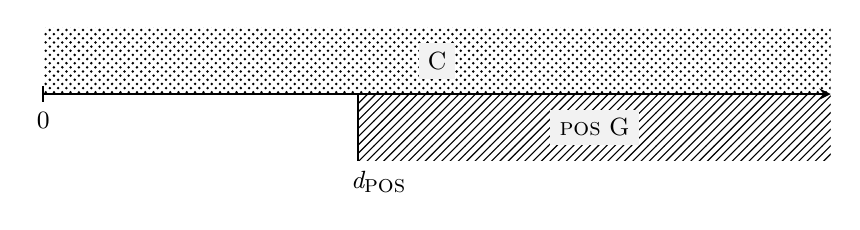
\begin{tikzpicture}
\draw[-stealth,line width=0.8pt] (0,0) -- (10,0);
\draw[line width=0.8pt] (0cm,3pt) -- (0cm,-3pt) node[anchor=north] {\small 0};
\draw[line width=0.8pt] (4cm,0pt) -- (4cm,-24pt) node[anchor=north] {\small $\textit{d}_{\rlap{\textsc{pos}}}$};
\path[pattern=north east lines, line width=0pt] (10cm,0) -- (4cm,0) -- (4cm,-24pt) -- (10cm,-24pt);
\path[pattern=crosshatch dots, line width=0pt] (10cm,0) -- (0cm,0) -- (0cm,24pt) -- (10cm,24pt);
\node[fill=black!5] at (7cm,-12pt) {\small \textsc{pos} G};
\node[fill=black!5] at (5cm,12pt) {\small C};
\end{tikzpicture}
\z

\ea   Intensität eines mittels \textit{sehr} modifizierten Intensivausdrucks:   \label{Pos001} \medskip

\centering
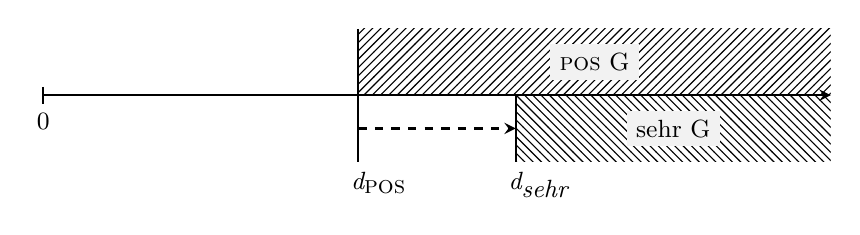
\begin{tikzpicture}
\draw[-stealth,line width=0.8pt] (0,0) -- (10,0);
\draw[line width=0.8pt] (0cm,3pt) -- (0cm,-3pt) node[anchor=north] {\small 0};
\draw[line width=0.8pt] (4cm,24pt) -- (4cm,-24pt) node[anchor=north] {\small $\textit{d}_{\rlap{\textsc{pos}}}$};
\draw[line width=0.8pt] (6cm,0pt) -- (6cm,-24pt) node[anchor=north] {\small $\textit{d}_{\rlap{\textit{sehr}}}$};
\draw[line width=0.8pt,dashed,-stealth] (4cm,-12pt) -- (6cm,-12pt);
\path[pattern=north east lines, line width=0pt] (10cm,0) -- (4cm,0) -- (4cm,24pt) -- (10.cm,24pt);
\path[pattern=north west lines, line width=0pt] (10cm,-24pt) -- (6cm,-24pt) -- (6cm,0pt) -- (10cm,0pt);
\node[fill=black!5] at (7cm,12pt) {\small \textsc{pos} G};
\node[fill=black!5] at (8cm,-12pt) {\small sehr G};
\end{tikzpicture}
\z

\newpage
\ea    Intensität eines mittels \textit{beinahe} modifizierten Intensivausdrucks: \label{Pos002} \medskip

\centering
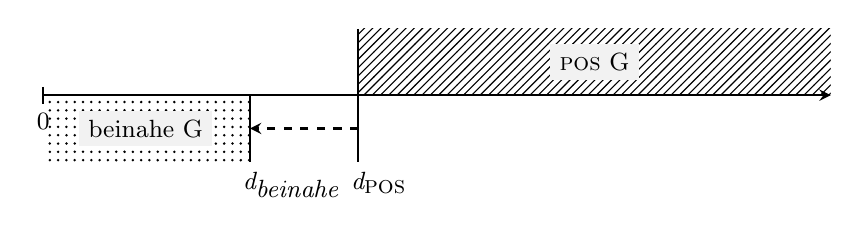
\begin{tikzpicture}
\draw[-stealth,line width=0.8pt] (0,0) -- (10,0);
\draw[line width=0.8pt] (0cm,3pt) -- (0cm,-3pt) node[anchor=north] {\small 0};
\draw[line width=0.8pt] (4cm,24pt) -- (4cm,-24pt) node[anchor=north] {\small $\textit{d}_{\rlap{\textsc{pos}}}$};
\draw[line width=0.8pt] (2.625cm,0pt) -- (2.625cm,-24pt) node[anchor=north] {\small $\textit{d}_{\rlap{\textit{beinahe}}}$};
\draw[line width=0.8pt,dashed,-stealth] (4cm,-12pt) -- (2.625cm,-12pt);
\path[pattern=north east lines, line width=0pt] (10cm,0) -- (4cm,0) -- (4cm,24pt) -- (10.cm,24pt);
\path[pattern= dots, line width=0pt] (0cm,-24pt) -- (2.625cm,-24pt) -- (2.625cm,0pt) -- (0cm,0pt);
\node[fill=black!5] at (7cm,12pt) {\small \textsc{pos} G};
\node[fill=black!5] at (1.3cm,-12pt) {\small beinahe G};
\end{tikzpicture}
\z

\noindent Wird ein graduierbares Adjektiv wie \textit{groß} mit einer Intensitätspartikel kombiniert, entsteht ein Intensivausdruck, der entweder in einem verstärkten Ausprägungsgrad wie in \REF{Pos001} oder einem abgeschwächten Ausprägungsgrad wie in \REF{Pos002} resultiert. Der Unterschied zwischen \textit{sehr} und \textit{beinahe} liegt in der Semantik der Ausdrücke: Ersterer wird stets mit einem hohen Intensitätsgrad verbunden, wohingegen letzterer vielmehr eine Annäherung an einen Referenzpunkt angibt und somit einen gemäßigteren {Intensitätsgrad ausdrückt}.

Syntaktisch zeichnen sich Intensitätspartikeln dadurch aus, dass sie weder koordinierbar noch flektierbar sind, also durch Eigenschaften, die sie bspw. mit Adverbien oder Präpositionen teilen. Ferner sind sie wie alle Partikeln nicht vorfeldfähig, können nicht Kopf einer Phrase sein und sich anders als Fokuspartikeln wie \textit{nur} oder \textit{bloß} in verstärkender Funktion nicht auf Nominalphrasen beziehen {\citep[vgl.][56]{Zifonun.1997}}.\footnote{Intensitätsmindernde Partikeln wie \textit{beinahe} oder \textit{nahezu} scheinen dagegen durchaus auf einer zugehörigen Nominalphrase operieren zu können, wie \citet[86]{Westpfahl.2020} bemerkt: Es ist \textit{\uline{nahezu ein Wunder}, dass Ted doch noch seine Traumfrau gefunden hat}.} Ihr Gebrauch ist im Allgemeinen nicht auf bestimmte grammatische Kategorien beschränkt. So lassen sich neben den in {Beispiel \REF{hochzeit0}} vorgeführten graduierbaren Adjektiven und Adverbien auch Nomen und Verben intensivieren. \citet[20ff.]{Laitenberger.2016} bespricht zudem die Intensivierbarkeit von Funktionsverbgefügen. Dies wird in Beispiel \REF{SynQuatsch} deutlich gemacht.

\ea  \label{SynQuatsch}
\ea Barney ist ein \textbf{absoluter Frauenheld}.  \label{marsh1}
\ex Robin hat die Moderation heute \textbf{völlig vergeigt}. \label{marsh2}
\ex Bei der Notenvergabe ist Marshall \textbf{arg ins Zittern geraten}. \label{marsh3}
 \z
 \z
Während der mit dem bewertenden Nomen \textit{Frauenheld} einhergehende Grad in Satz \REF{marsh1} durch den Intensivierer \textit{absolut} funktional gesteigert wird, erhält das Partizip \textit{vergeigt} in Satz \REF{marsh2} durch \textit{völlig} eine skalare Komponente. Dadurch wird ausgedrückt, dass die Sendung für Robin nicht hätte schlechter laufen können bzw. auf einer Skala des Gelingens kaum ein niedrigerer Wert erreicht werden kann. Als notwendige Voraussetzung für die Intensivierbarkeit von Nomen und Verben erklären {\citet[292]{Hentschel.2013}}, dass die ausgedrückte Eigenschaft bzw. Handlung inhärent variabel und somit steigerbar sein muss: So kann Marshall zwar ein \textit{totaler Chaot} sein, Ted aber nicht ein \textit{totaler Architekt}. Gleichsam kann man ein leckeres Abendessen zwar \textit{sehr genießen}, ein spannendes Buch jedoch nicht \textit{sehr lesen} {\citep[vgl.][292]{Hentschel.2013}}. Hinsichtlich der Intensivierbarkeit von Verbkonstruktionen kommt \citet[21]{Laitenberger.2016} zu dem Schluss, dass bei einem Funktionsverbgefüge wie dem obigen vornehmlich das Nomen von Bedeutung ist, das die Dimension der Skala vorgibt: In Satz \REF{marsh3} ist die Intensivierung des Funktionsverbgefüges so zu verstehen, dass der Grad, zu dem Marshall gezittert hat, einen für solche Situationen vergleichbaren Grad, den hier einschlägigen Vergleichsstandard also, bei Weitem übersteigt.



\subsubsection{Die Einteilung in deskriptiv und expressiv} \label{Intensivierertypen}
Die in Abschnitt \ref{DeEx} getroffene Unterscheidung zwischen deskriptivem und expressivem Bedeutungstyp kann auch auf die Funktionsklasse der Intensivierer angewandt werden: So zerfällt diese ebenfalls in zwei Parteien, deren Hauptmerkmal die Klassifikation nach deskriptiv oder expressiv ist. Mit dieser Klassifikation befasst sich der folgende Abschnitt. Begonnen wird mit den Wesensmerkmalen der deskriptiven Intensivierer, woran sich eine Begutachtung der expressiven Intensivierer sowie eine Gegenüberstellung beider Klassen in Hinsicht auf Gemeinsamkeiten und Unterschiede anschließt.

\subsubsubsection{Deskriptive Intensivierer}
\largerpage

Die Klasse der deskriptiven Intensivierer kann als relativ stabil bezeichnet werden, handelt es sich doch um ein fest etabliertes Inventar an Kernausdrücken wie \textit{äußerst}, \textit{außerordentlich} oder \textit{überaus}, ohne dass sich der Umfang wahrnehmbar vergrößert oder verkleinert. In der theoretischen Literatur wird sie zumeist durch die deutsche Standard-Intensitätspartikel \textit{sehr} beschrieben, auf der auch in diesem Abschnitt der Fokus liegt. Da deskriptive Intensivierer delexikalisiert, dadurch konnotationslos, und neutral skalierend sind, liegt ihr semantischer Beitrag ausschließlich darin, dem Ausprägungsgrad des Prädikats eine höhere Skalenposition zuzuschreiben (vgl. Abschnitt {\REF{Funktionsklasse}}).  \citet[132f.]{Gutzmann.2019a}, der die Bedeutung eines graduierbaren Adjektivs exemplarisch an \textit{cool} als \glqq{}relation between a {degree \textit{d}} and an {entity \textit{x}} such that the coolness of \textit{x} equals \textit{d}\grqq{} definiert, beschreibt den semantischen Unterschied zwischen dem unmarkierten Positiv und \textit{sehr} (stellvertretend für die Klasse der deskriptiven Intensivierer) in Anlehnung an {\citet[370]{Kennedy.2005}} formal wie folgt:\footnote{\citet[133]{Gutzmann.2019a} zeigt die Semantik deskriptiver Intensivierer am Beispiel des englischen \textit{very} auf, was hier aus Analogiegründen auf das deutsche \textit{sehr} übertragen wird.}  \medskip

\noindent
$\lsem$\textbf{pos}$\rsem$ = $\lambda$\textit{G}$\lambda$\textit{x}. there is a degree \textit{d}, such that \textit{d} meets the standard given by
the comparison class \textit{C} and \textit{x} is \textit{G} to degree \textit{d}. \medskip

\noindent
$\lsem$\textbf{very}$\rsem$ = $\lambda$\textit{G}$\lambda$\textit{x}. there is a degree \textit{d}, such that \textit{d} meets the standard given by
the comparison class $\lambda$\textit{y}.$\lsem$\textbf{pos}(\textit{G})(\textit{y})$\rsem$ and \textit{x} is \textit{G} to degree \textit{d}
given by the comparison class $\lambda$\textit{y}.$\lsem$\textbf{pos}(\textit{G})(\textit{y})$\rsem$ and \textit{x} is \textit{G} to degree \textit{d}. 
\medskip

\noindent Wie schon im Hinblick auf die obigen skalaren Darstellungen \REF{Pos000} bis \REF{Pos002} erläutert, verbirgt sich hinter diesen beiden Definitionen von {\citet[132f.]{Gutzmann.2019a}} die Idee, dass die Einschätzung des Grades \textit{d} auf der Skala relativ zu einer Vergleichsklasse \textit{C} erfolgt. Auch hier steht der {Positiv \textit{G}} für eine beliebige Eigenschaft (bspw. \textit{groß}) und \textit{d} für den Grad, den ein Gegenstand \textit{x} in Bezug auf diese Eigenschaft erfüllen muss, damit ihm \textit{G} zugesprochen wird. In diesem Sinne bezeichnet man eine Frau mit einer Körpergröße von 153\,cm kaum als groß, da sie deutlich unter der vom Statistischen Bundesamt ermittelten Durchschnittsgröße deutscher Frauen liegt.\footnote{Die Körpergröße deutscher Frauen betrug im letzten Erhebungszeitraum 2008 bis 2011 laut Statistischem Bundesamt durchschnittlich 163,5\,cm (vgl. \citealt[]{Statistik.2020}, [letzter Aufruf: 06.06.2022]).} Liegt die Körpergröße einer Frau jedoch weit über dem Durchschnittswert von 163,5\,cm, etwa bei {173\,cm}, so ist man eher dazu geneigt, die Frau -- relativ zum Vergleichsstandard -- als groß zu bezeichnen. Im Falle des Positivs \textit{groß} stellt die Durchschnittsgröße die Vergleichsklasse dar, anhand derer die Einordnung des Gegenstands auf der Skala erfolgt (vgl. die Skala {zu \REF{Pos01})}.

\ea  Intensität eines intensivierbaren Adjektivs im Positiv: \medskip

\centering

\label{Pos01}
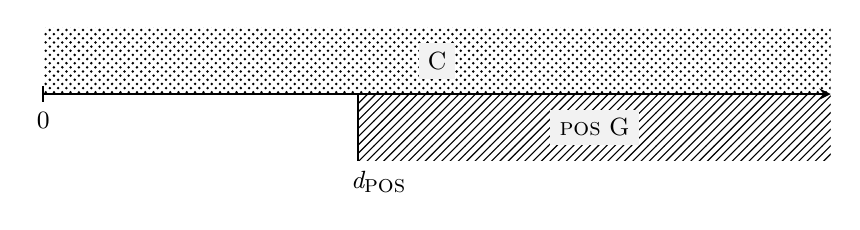
\begin{tikzpicture}
\draw[-stealth,line width=0.8pt] (0,0) -- (10,0);
\draw[line width=0.8pt] (0cm,3pt) -- (0cm,-3pt) node[anchor=north] {\small 0};
\draw[line width=0.8pt] (4cm,0pt) -- (4cm,-24pt) node[anchor=north] {\small $\textit{d}_{\rlap{\textsc{pos}}}$};
\path[pattern=north east lines, line width=0pt] (10cm,0) -- (4cm,0) -- (4cm,-24pt) -- (10cm,-24pt);
\path[pattern=crosshatch dots, line width=0pt] (10cm,0) -- (0cm,0) -- (0cm,24pt) -- (10cm,24pt);
\node[fill=black!5] at (7cm,-12pt) {\small \textsc{pos} G};
\node[fill=black!5] at (5cm,12pt) {\small C};
\end{tikzpicture}
\z

\largerpage
\noindent In der Definition des deskriptiven Intensivierers \textit{sehr} nach {\citet[132f.]{Gutzmann.2019a}} bezieht sich die Vergleichsklasse $\lambda$\textit{y}.$\lsem$\textbf{pos}(\textit{G})(\textit{y})$\rsem$ auf all diejenigen Gegenstände, die auf der Skala oberhalb des {Grades \textit{d}} anzusiedeln sind. Demnach ergibt sich der Vergleichsstandard des Intensivausdrucks \textit{sehr groß} aus der Menge aller Frauen, die aufgrund einer überdurchschnittlichen Körpergröße die Eigenschaft haben, groß zu sein. Überschreitet die Größe einer Frau den Durchschnittswert dieser Vergleichsklasse stark, weil sie bspw. 183\,cm groß ist, so ist der Grad der bezeichneten Eigenschaft notwendigerweise höher zu positionieren als der in der Definition des Positivs \textit{groß} spezifizierte Grad. Die daraus folgende Verschiebung auf der Skala führt zu einer Verengung des Begriffsumfangs, da die Eigenschaft infolge der Modifikation durch \textit{sehr} auf weniger Gegenstände zutrifft: Es gibt einfach weniger Frauen, deren Körpergröße von der hier einschlägigen Vergleichsklasse, d.\,h. von der Menge großer Frauen ausgehend derart stark nach oben abweicht (vgl. die Skala {zu \REF{ska})}.


\ea  Intensität eines mittels \textit{sehr} modifizierten Intensivausdrucks: \medskip

\centering \label{ska}
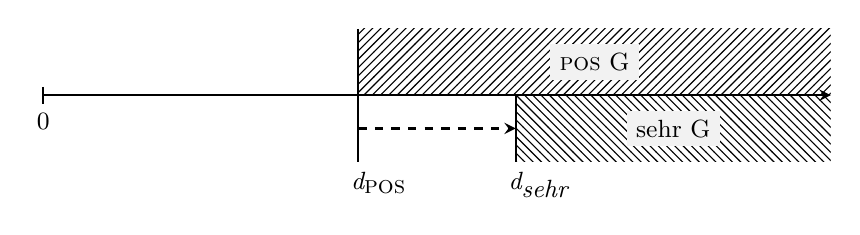
\begin{tikzpicture}
\draw[-stealth,line width=0.8pt] (0,0) -- (10,0);
\draw[line width=0.8pt] (0cm,3pt) -- (0cm,-3pt) node[anchor=north] {\small 0};
\draw[line width=0.8pt] (4cm,24pt) -- (4cm,-24pt) node[anchor=north] {\small $\textit{d}_{\rlap{\textsc{pos}}}$};
\draw[line width=0.8pt] (6cm,0pt) -- (6cm,-24pt) node[anchor=north] {\small $\textit{d}_{\rlap{\textit{sehr}}}$};
\draw[line width=0.8pt,dashed,-stealth] (4cm,-12pt) -- (6cm,-12pt);
\path[pattern=north east lines, line width=0pt] (10cm,0) -- (4cm,0) -- (4cm,24pt) -- (10.cm,24pt);
\path[pattern=north west lines, line width=0pt] (10cm,-24pt) -- (6cm,-24pt) -- (6cm,0pt) -- (10cm,0pt);
\node[fill=black!5] at (7cm,12pt) {\small \textsc{pos} G};
\node[fill=black!5] at (8cm,-12pt) {\small sehr G};
\end{tikzpicture}
\z

In der theoretischen Literatur wird grundsätzlich die Auffassung vertreten, dass \textit{sehr} im Unterschied zu polyfunktionalen Intensivierern wie z.\,B. \textit{ganz}, die gleichermaßen intensitätsverstärkend wie auch intensitätsabschwächend fungieren können,\footnote{Im Hinblick auf \textit{ganz} merken \citet[31]{Pusch.1981} und \citet[136f.]{Os.1989} an, dass es in Abhängigkeit von Adjektivtyp und Betonung sowohl bedeutungsverstärkend (mit Betonung) im aufwertenden Sinne von `völlig' oder `total' als auch -abschwächend (ohne Betonung) im abwertenden Sinne von `leidlich' oder `einigermaßen' verwendet werden kann. Ähnliches besprechen \citet[400]{Stratton.2022} im Hinblick auf die norwegische Partikel \textit{ganske}, die -- ebenso wie \textit{ganz} -- ein Kognat des englischen \textit{quite} ist.} nicht funktionsambig ist: Es hat ausschließlich die Verstärkung des Prädikats zur Folge (vgl. u.\,a. \citealt[31]{Pusch.1981}; {\citealt[194]{Os.1989}}; \citealt[589]{Duden.2016}). Trotz der verstärkenden Intensität weist {\citet[7]{Mueller.1899}} darauf hin, dass \textit{sehr} als ältester Intensivierer pragmatisch kaum aussagekräftig ist. Stattdessen bedürfe es anderer, d.\,h. expressiver Ausdrücke, um eine Äußerung nachdrücklicher zu machen. So sei es in früheren Zeitstufen sogar üblich gewesen, \textit{sehr} in seiner Gradbedeutung in Gestalt von \glqq{}serner\grqq{} zu steigern, was seinerzeit allerdings nur noch in mündlichkeitsnahen Sprachvarietäten möglich gewesen sei \citep[vgl.][7]{Mueller.1899}. Unterdessen lässt sich die Verstärkung von \textit{sehr} allenfalls durch Reduplikation erzielen, wie \citet[191]{Staffeldt.2018} unterstreicht: \textit{Ted ist sehr, sehr aufgeregt}.


Syntaktisch kann \textit{sehr} neben adjazenten prädikativen \REF{ted01} ebenso {attributive \REF{ted02}} und adverbiale Adjektive \REF{ted003} verstärken, wie die modifizierten Sätze aus dem obigen Beispiel \REF{ted0} zeigen:

\ea   \label{ted00}
\ea Ted ist vor seiner Hochzeit \textbf{sehr aufgeregt}. \label{ted01}
\ex Der \textbf{sehr aufgeregte} Ted trinkt einen Schnaps. \label{ted02}
\ex Ted trippelt \textbf{sehr aufgeregt} von einem Raum zum nächsten. \label{ted003}
 \z
 \z
Bemerkenswert ist die sprachgeschichtliche Entwicklung, die \textit{sehr} über die Zeit vollzogen hat. Nach \citet[1270f.]{Pfeifer.1995} ist anzunehmen, dass es im Mittelhochdeutschen erstmals in intensivierender Funktion verwendet wurde. Während es anfangs in Konkurrenz mit anderen Ausdrücken stand, gelang es ihm jedoch, sich sukzessive gegen diese durchzusetzen und sich mit der Bedeutung von `schwer' dauerhaft als Intensitätspartikel zu etablieren \citep[vgl.][266]{Becher.1907}. Interessant ist dabei aber vor allem der lexikalische Ursprung, der mittlerweile vollkommen opak und den wenigsten Muttersprachler:innen bewusst ist: Wie viele Intensivierer stammt auch \textit{sehr} von einem Adjektiv ab, das einerseits aufgrund einer bestehenden Lücke im Inventar und andererseits dank seiner negativen Bedeutung in die Intensiviererrolle übernommen wurde. So führt \citet[1270f.]{Pfeifer.1995} den etymologischen Ursprung von \textit{sehr} auf das althochdeutsche Adjektiv \textit{sēro} zurück, das im 9. Jahrhundert im Sinne von `mit Schmerz, schmerzlich, traurig, betrübt, hart' gebraucht wurde und diese negative Bedeutungskomponente bis ins Mittelhochdeutsche hinein beibehielt. In dieser Zeitstufe löste es sich von seinem ursprünglichen Bedeutungsgehalt ab und nahm eine allgemeinere Gradbedeutung an (vgl. {\citealt[7]{Mueller.1899}}; \citealt[185f.]{Kip.1900}). \citet[1270f.]{Pfeifer.1995} ist überdies zu entnehmen, dass \textit{sehr} etymologisch mit dem englischen \textit{sore} verwandt ist, das heute noch mit `schlimm, wund, verletzt' übersetzt wird und direkten Bezug zu seiner negativen Herkunft aufweist.\footnote{Auch der heutige Ausdruck \textit{sorry} (im Sinne von `Entschuldigung') ist etymolgisch mit dem englischen Intensivierer \textit{sore} verwandt; beide gehen historisch auf die Bedeutung `pain(ful)' zurück (vgl. \citealt[191f.]{Stratton.2020b};; {\citealt[212]{Stratton.2020c}}).} Dies zeigt, dass \textit{sehr} typischerweise nicht nur adjektivischen, sondern ebenso emotional-expressiven Ursprungs ist, wie u.\,a. \citet[33]{Pustka.2014b} illustriert. Mit der Zeit und fortschreitender Desemantisierung\footnote{Laut \citet[264]{Bechmann.2016} meint Desemantisierung das \glqq{}Verblassen der ursprünglichen Bedeutung bis hin zum vollständigen Verlust der konkreten Bedeutung\grqq{}. Dieser Prozess gilt als charakteristisch für die Entwicklung syntaktischer Elemente {\citep[vgl.][363]{Claudi.2006}}.} hat \textit{sehr} seinen ursprünglichen semantischen Gehalt und somit auch seine Expressivität gänzlich eingebüßt, was dazu führte, dass es inzwischen lediglich als neutral skalierend wahrgenommen wird: \glqq{}[I]ntensifiers tend to lose their semantic specificities by frequent use, and as their meaning fades, their only function is to express degree, thus becoming purely scalar intensifiers.\grqq{} (\citealt[379]{Mendez-Naya.2003}). Hinweise auf die ehemals negative Bedeutung des Ursprungslexems finden sich heute nur noch in {\textit{(un-)ver\uline{sehr}t}}, was gemeinhin {`(un)verletzt'} bedeutet.\footnote{Für eine Diskussion dieses Lexems in anderen frühgermanischen Sprachen (bspw. Niederländisch und Isländisch) sei auf \citet[191f.]{Stratton.2020b} verwiesen.} Neben \textit{sehr} haben auch andere -- deutsche wie englische -- Intensitätspartikeln eine solche semantische Entwicklung durchlaufen. Hierzu gehören u.\,a. \textit{arg} oder \textit{furchtbar} (vgl. \citealt[182ff.]{Kirschbaum.2002b};; \citealt[191ff.]{Stratton.2020c}).

Semantisch entleerte Intensivierer lassen sich zusätzlich zu Adjektiven der gleichen Polarität auch mit semantisch gegenläufigen Adjektiven kombinieren: Je stärker ein Intensivierer desemantisiert sei, desto weiter dehne sich sein Anwendungsbereich aus, was gleichzeitig in einem Anstieg in der Verwendung resultiere {\citep[vgl.][420]{Breindl.2007}}. Aufgrund dieser Entwicklung hat \textit{sehr} nunmehr bloß verstärkende Funktion und kann infolge der starken Einbuße an semantischen und morphosyntaktischen Eigenschaften zudem als am stärksten grammatikalisiert angesehen werden: \glqq{}Unser \glq{}sehr\grq{} bedeutet ursprünglich \glq{}schmerzlich\grq{} (vgl. versehren), und welch ein abstraktes Nichts ist es heute!\grqq{} (\citealt[2]{Hauschild.1899}). Durch den fehlenden expressiven Gehalt wird es grundsätzlich als moderat verstärkend wahrgenommen, weshalb es \citet[365]{Claudi.2006} als \glqq{}half-hearted intensification\grqq{} bezeichnet. Als Konsequenz daraus lässt sich \textit{sehr} problemlos in allen Kontexten verwenden -- und fungiert damit als Universalmittel der deutschen Adjektiv-Intensivierung.


\subsubsubsection{Expressive Intensivierer}

Der deskriptiven gegenüber steht die erheblich heterogenere und weniger klar abgegrenzte Klasse der expressiven Intensivierer, die verschiedene Sprachvarietäten vereint und zu der u.\,a. \textit{krass}, \textit{sau} und \textit{übel(st)} gehören. Wie {\citet[650]{Bussmann.2002}} erklärt, zeichnet sich diese Intensiviererklasse insbesondere durch einen ständigen Wandel aus, der der Affektivität der Ausdrücke geschuldet sei.\footnote{Es ist anzunehmen, dass der Wandel im lexikalischen Inventar nicht bloß der Diachronie geschuldet ist, sondern dass alle neuen Intensivierer von der Sprechergemeinschaft zunächst als expressiv wahrgenommen werden, mit zunehmendem oder längerem Gebrauch jedoch delexikalisiert und schließlich nur noch als deskriptiv verstärkend {empfunden werden}.} Die Tatsache, dass expressive Intensivierer dieselben Verwendungsweisen haben wie deskriptive Intensivierer, zeigt, dass es sich bei ihnen ebenfalls um Gradausdrücke mit primär kommunikativ-pragmatischer Funktion handelt. Doch aus welchen Gründen greifen Sprecher unter bestimmten Bedingungen überhaupt darauf zurück? Die Antwort auf diese Frage findet sich u.\,a. in \citet[]{Berz.1953}:

\begin{quotation} \noindent Wer \textit{steinhart} statt \textit{sehr h.}, \textit{steinreich} für \textit{sehr r.}, \textit{steinalt} oder gar \textit{hundalt} für \textit{sehr a.} oder \textit{ganz a.} gebraucht, der hat zu diesen Ausdrücken gegriffen, weil ein gefühlsbetonter Sach- oder Situationsverhalt ihn dazu drängte, sich sprachlich abzureagieren.
\hfill (\citealt[17f.]{Berz.1953})  \end{quotation}

\noindent Auch wenn sich die Untersuchungen von \citet[]{Berz.1953} hauptsächlich auf Steigerungskomposita wie das von ihm erwähnte \textit{steinhart} und weniger auf Intensitätspartikeln konzentrieren, lassen sich dennoch klare Parallelen hinsichtlich der Motivation erkennen. So wird gemeinhin davon ausgegangen, dass expressive Intensivierer ebenso wie die bezeichneten Steigerungskomposita im Vergleich zu deskriptiven Intensivierern neben der eigentlichen Verstärkung auch die evaluative Einstellung des Sprechers gegenüber einer (möglichen) Situation, einem Sachverhalt oder einem Objekt in der Welt kommunizieren (vgl. bspw. \citealt[315]{Lang.1983} und \citealt[57]{Ortner.2014}). Demzufolge beinhaltet eine Äußerung mit expressivem Ausdruck in der Regel zwei Bedeutungstypen: zum einen den wahrheitswertfähigen deskriptiven Gehalt, der jeder neutralen Äußerung zugrunde liegt, sowie zum anderen eine additive emotional-expressive Komponente, die den propositionalen Gehalt um eine evaluative sprecherbezogene Stellungnahme erweitert {\citep[vgl.][134f.]{Gutzmann.2019a}}. Nachfolgend wird der semantische Unterschied zwischen dem unmarkierten Positiv und \textit{sau} (stellvertretend für die Klasse der expressiven Intensivierer) nach {\citet[133]{Gutzmann.2019a} beschrieben:} \medskip

\noindent
$\lsem$\textbf{pos}$\rsem$ = $\lambda$\textit{G}$\lambda$\textit{x}. there is a degree \textit{d}, such that \textit{d} meets the standard given by the comparison class \textit{C} and \textit{x} is \textit{G} to degree \textit{d}. \medskip

\noindent
$\lsem$\textbf{sau}$\rsem$ = $\lambda$\textit{G}$\lambda$\textit{x}. there is a degree \textit{d}, such that \textit{d} meets the standard given by the comparison class $\lambda$\textit{y}.$\lsem$\textbf{very}(\textit{G})(\textit{y})$\rsem$ and \textit{x} is \textit{G} to degree \textit{d}. 
\medskip

\noindent Analog zum obigen Vorgehen wird auch diese Definition exemplarisch am graduierbaren Adjektiv \textit{groß} veranschaulicht. Wie zuvor erläutert, ergibt sich die Vergleichsklasse \textit{C} bei einem deskriptiven Intensivierer wie \textit{sehr} laut {\citet[133]{Gutzmann.2019a}} aus der Menge aller Gegenstände, die auf der Skala oberhalb des Grades \textit{d} zu verorten sind. Bezogen auf das Beispiel bezieht sich der Vergleichsstandard somit auf all diejenigen Frauen, die infolge überdurchschnittlicher Körpergröße von bspw. 173\,cm gemäß der Definition des Positivs \textit{groß} über die Eigenschaft verfügen, groß zu sein (vgl. Skala zu \REF{ska01}).

\ea  Intensität eines mittels \textit{sehr} modifizierten Intensivausdrucks: \medskip

\centering \label{ska01}
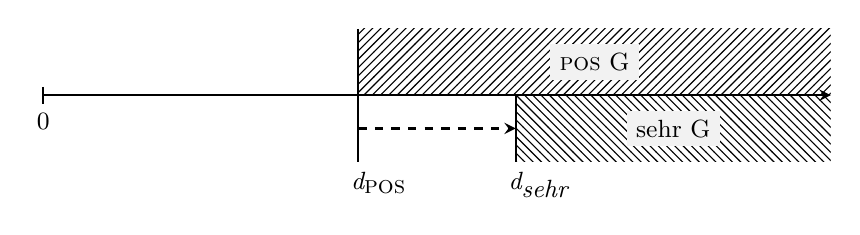
\begin{tikzpicture}
\draw[-stealth,line width=0.8pt] (0,0) -- (10,0);
\draw[line width=0.8pt] (0cm,3pt) -- (0cm,-3pt) node[anchor=north] {\small 0};
\draw[line width=0.8pt] (4cm,24pt) -- (4cm,-24pt) node[anchor=north] {\small $\textit{d}_{\rlap{\textsc{pos}}}$};
\draw[line width=0.8pt] (6cm,0pt) -- (6cm,-24pt) node[anchor=north] {\small $\textit{d}_{\rlap{\textit{sehr}}}$};
\draw[line width=0.8pt,dashed,-stealth] (4cm,-12pt) -- (6cm,-12pt);
\path[pattern=north east lines, line width=0pt] (10cm,0) -- (4cm,0) -- (4cm,24pt) -- (10.cm,24pt);
\path[pattern=north west lines, line width=0pt] (10cm,-24pt) -- (6cm,-24pt) -- (6cm,0pt) -- (10cm,0pt);
\node[fill=black!5] at (7cm,12pt) {\small \textsc{pos} G};
\node[fill=black!5] at (8cm,-12pt) {\small sehr G};
\end{tikzpicture}
\z

\noindent Im Gegensatz dazu besteht die Vergleichsklasse $\lambda$\textit{y}.$\lsem$\textbf{very}(\textit{G})(\textit{y})$\rsem$ bei expressiven Intensivierern wie \textit{mega} oder \textit{sau} {\citet[133]{Gutzmann.2019a}} zufolge aus der Durchschnittsgröße der Menge aller Gegenstände, die man aufgrund ihres Ausprägungsgrades als \textit{sehr groß} bezeichnen würde. Beträgt die Körpergröße einer Frau also z.\,B. 195 cm, so ist der Grad \textit{g} auf der Skala über dem Vergleichsstandard, d.\,h. dem Durchschnittswert sehr großer Frauen, zu verorten, was eine stärkere Verschiebung auf der Skala und einen engeren Begriffsumfang als den durch die Modifikation mittels \textit{sehr} entstehenden nach sich zieht: Es gibt einfach noch weniger Frauen, deren Größe von dem hier einschlägigen Vergleichsstandard, d.\,h. von der Menge sehr großer Frauen ausgehend derart stark nach oben abweicht (vgl. Skala zu \REF{ska2}).

\ea  Intensität eines mittels \textit{mega} modifizierten Intensivausdrucks: \medskip

\centering  \label{ska2}
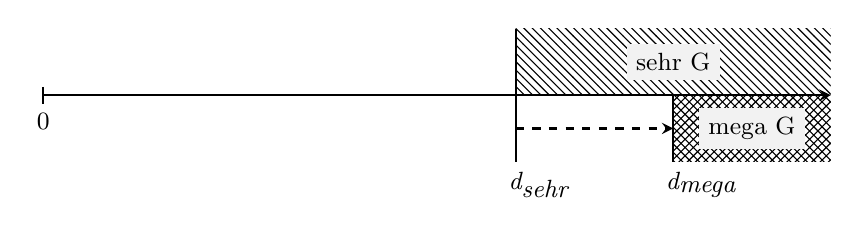
\begin{tikzpicture}
\draw[-stealth,line width=0.8pt] (0,0) -- (10,0);
\draw[line width=0.8pt] (0cm,3pt) -- (0cm,-3pt) node[anchor=north] {\small 0};
\draw[line width=0.8pt] (6cm,24pt) -- (6cm,-24pt) node[anchor=north] {\small $\textit{d}_{\rlap{\textit{sehr}}}$};
\draw[line width=0.8pt] (8cm,0pt) -- (8cm,-24pt) node[anchor=north] {\small $\textit{d}_{\rlap{\textit{mega}}}$};
\draw[line width=0.8pt,dashed,-stealth] (6cm,-12pt) -- (8cm,-12pt);
\path[pattern=north west lines, line width=0pt] (10cm,0pt) -- (6cm,0pt) -- (6cm,24pt) -- (10cm,24pt);
\path[pattern=crosshatch, line width=0pt] (10cm,0pt) -- (8cm,0pt) -- (8cm,-24pt) -- (10cm,-24pt);
\node[fill=black!5] at (8cm,12pt) {\small sehr G};
\node[fill=black!5] at (9cm,-12pt) {\small mega G};
\end{tikzpicture}
\z

Syntaktisch können expressive Intensivierer genauso wie deskriptive Intensivierer adjazente prädikativ, attributiv und adverbial verwendete Adjektive verstärken.\footnote{Im Hinblick auf die syntaktischen Verwendungsweisen von Intensivierern findet sich in der Literatur die Annahme, dass Intensivierer, die häufiger in attributiver Position auftreten, stärker delexikalisiert sind als prädikativ gebrauchte Intensivierer (vgl. {\citealt[271]{Ito.2003}}; \citealt[373]{Tagliamonte.2008}; \citealt[116]{Tagliamonte.2014}).} Beispiel \REF{Expr0} beinhaltet verschiedene expressive Intensivierer, die gegenwärtig vor allem bei jüngeren Sprecher:innen gebräuchlich sind.

\ea  \label{Expr0}
\ea Marshall: \glqq{}Lily ist \textbf{krass gut} im Zeichnen.\grqq{} \label{lily}
\ex Robin: \glqq{}Marshall ist ein \textbf{mega netter} Anwalt.\grqq{}  \label{GNB1}
\ex Ted: \glqq{}Barneys neuer Smoking sieht \textbf{übelst schick} aus.\grqq{}  \label{Anzug}
 \z
 \z
Während Satz \REF{lily} abgesehen von der reinen Beschreibung, dass Lily ein ausgeprägtes künstlerisches Talent hat, weiterhin inhärent die Bewunderung des Sprechers beinhaltet, geben die Intensivausdrücke in {\REF{GNB1} und \REF{Anzug}} über die Sachverhaltsbeschreibung hinaus gleichfalls die Anerkennung des Sprechers gegenüber Marshalls Charaktereigenschaft bzw. Barneys Smoking wieder. In den Sätzen zeigt sich somit, dass der Intensivierer die durch das Adjektiv ausgesagte Eigenschaft in hohem Maße steigert, wodurch der Intensivausdruck nach Auffassung von \citet[22]{Paradis.1997} und {\citet[133]{Gutzmann.2019a}} eine höhere Skalenposition erhält als eine unmarkierte oder mittels \textit{sehr} intensivierte Variante. Gleichzeitig wird die subjektive Einstellung des Sprechers kommuniziert, die nicht Teil des deskriptiven Gehalts ist, wie u.\,a. \citet[10]{Paradis.1997} und {\citet[560]{Athanasiadou.2007}} erläutern. In diesem Sinne lassen sich sowohl die Skalarität, die den Ausprägungsgrad des Prädikats angibt, als auch die implizit ausgedrückte Sprechereinstellung auf einer Skala verorten. Je höher das Intervall auf der Skala liegt, desto ausgeprägter ist das in der Äußerung beschriebene Merkmal sowie die damit verbundene Sprecherhaltung einzuschätzen. Die zugrunde liegende Annahme der beiden voneinander unabhängigen Bedeutungsdimensionen wird unter Zuhilfenahme der von {\citet[5]{Gutzmann.2013a}} eingeführten Notation am Beispiel des {Satzes \REF{lily} vorgeführt}: \medskip

\noindent Lily ist krass gut im Zeichnen = \begin{large} $\frac{\text{Der Sprecher bewundert Lilys künstlerisches Talent}}{\text{Lily ist sehr, sehr gut im Zeichnen}}$ \end{large}
\medskip

\noindent Die Konklusion als Basis entspricht dem deskriptiven Bedeutungsgehalt der Äußerung,\footnote{Zu beachten ist, dass das reduplizierte \textit{sehr} lediglich  eine Approximation an den deskriptiven Gehalt eines expressiven Intensivierers darstellt. Da deskriptive Intensivierer nach \citet[133]{Gutzmann.2019a} weniger ausdrucksstark sind als expressive Intensivierer, scheint bloß \textit{sehr, sehr} ansatzweise dazu geeignet, um die deskriptive Bedeutung von {\textit{krass} anzugeben.}} wohingegen die Prämisse die Haltung des Sprechers zum bezeichneten Sachverhalt anzeigt, die laut \citet[20f.]{Gutzmann.2015a} auf einer zusätzlichen emotional-expressiven Ebene angesiedelt ist. Dementsprechend lässt sich die deskriptive Bedeutung des Satzes \textit{Lily ist krass gut im Zeichnen} sich in etwa als \textit{Lily ist so gut im Zeichnen, dass ihr künstlerisches Talent die einschlägige Norm bei Weitem überschreitet} paraphrasieren. Der expressiven Bedeutung gemäß drückt der Sprecher in der Äußerungssituation seine persönliche Einstellung gegenüber Lilys Talent und der besagten Normüberschreitung  aus. Diese subjektive Komponente wird auf deskriptiver Ebene nicht overt kommuniziert, sondern befindet sich in Gutzmanns Schema auf einer zweiten Ebene und kann sich grundsätzlich in unterschiedlichen affektiven Qualitäten (z.\,B. Bewunderung, Eifersucht oder {Überraschung) manifestieren}.

Basierend auf den soeben vorgestellten theoretischen Annahmen lässt sich daher zusammenfassen, dass expressive Intensivierer mit einem höheren Skalaritätsgrad einhergehen als deskriptive Intensivierer und infolgedessen eine stärkere Verschiebung von Graden auf einer
Skala bewirken (vgl. {\citealt[22]{Paradis.1997}}; \citealt[133]{Gutzmann.2019a}). Außerdem haben sie eine kommunikativ-pragmatische Funktion, die auf einer separaten Bedeutungsebene verankert ist. Durch die expressive Zusatzkomponente ist der Sprecher offenbar in der Lage, neben der Sachverhaltsbeschreibung auch seine evaluative Haltung gegenüber der thematisierten Sachlage kundzutun (vgl. \citealt[315]{Lang.1983}; {\citealt[57]{Ortner.2014}}).\footnote{Die Gültigkeit dieser Annahmen wird in den Kapiteln \REF{Experiment0} und \REF{Experimente} experimentell untersucht.} Vor diesem Hintergrund erläutert {\citet[136]{Gutzmann.2019a}}, dass es sich bei expressiven Intensivierern um Ausdrücke handelt, die zwei Bedeutungsebenen vereinen: die intensivierende Dimension (= \glqq{}intensifying aspect\grqq{}, hier und im Folgenden abgekürzt mit \textit{int}) als Teil des wahrheitswertfähigen deskriptiven Gehalts sowie die gebrauchsbedingte evaluative Dimension (= \glqq{}expressive attitude\grqq{}, hier und im Folgenden abgekürzt mit \textit{emo}), auf der die subjektive Einstellung des Sprechers angesiedelt ist. Die Verknüpfung beider Ebenen demonstriert er unter Anwendung des von ihm eingeführten Diamant-Operators ({{\larger[-1]\ding{117}}}) stellvertretend für alle expressiven Intensivierer an der Bedeutung von \textit{sau}: \medskip


\noindent
\textbf{sau} = $\lambda$\textit{G}$\lambda$\textit{x}.\textbf{int}(\textit{G})(\textit{x})\,:\,$\langle$$\langle$\textit{d},\,$\langle$\textit{e},\,\textit{t}$\rangle$$\rangle$,\,$\langle$\textit{e},\,\textit{t}$\rangle$$\rangle$ {{\larger[-1]\ding{117}}} $\lambda$\textit{G}$\lambda$\textit{x}.\textbf{emo}(\textit{G})(\textit{x})\,:\,$\langle$$\langle$\textit{d},\,$\langle$\textit{e},\,\textit{t}$\rangle$$\rangle$,\,$\langle$\textit{e},\,\textit{u}$\rangle$$\rangle$.
\medskip

\noindent Davon ausgehend modelliert \citet[136]{Gutzmann.2019a} die beiden semantischen Ebenen von expressiven Intensivierern auf folgende Weise: \medskip

\noindent
$\lsem$\textbf{int}$\rsem$ = $\lambda$\textit{G}$\lambda$\textit{x}. there is a degree \textit{d}, such that \textit{d} meets the standard given by the comparison class $\lambda$.$\lsem$\textbf{very}(\textit{G})(\textit{y})$\rsem$ and \textit{x} is \textit{G} to degree \textit{d}\,:\,$\langle$$\langle$\textit{d},\,$\langle$\textit{e},\,\textit{t}$\rangle$$\rangle$,\,$\langle$\textit{e},\,\textit{t}$\rangle$$\rangle$.
\medskip

\noindent
$\lsem$\textbf{emo}$\rsem$ = $\lambda$\textit{G}$\lambda$\textit{x}. the speaker \textit{c}\textsubscript{\textit{S}} is emotional about the fact that there is a degree \textit{d} such that \textit{d} meets the standard given by the comparison class $\lambda$.$\lsem$\textbf{very}(\textit{G})(\textit{y})$\rsem$ and \textit{x} is \textit{G} to degree \textit{d}\,:\,$\langle$$\langle$\textit{d},\,$\langle$\textit{e},\,\textit{t}$\rangle$$\rangle$,\,$\langle$\textit{e},\,\textit{u}$\rangle$$\rangle$.
\medskip

\noindent Die von \citet[136]{Gutzmann.2019a} vorgeschlagene Definition für die beiden voneinander unabhängigen Bedeutungsdimensionen expressiver Intensivierer wie \textit{mega} oder \textit{sau} sind wie folgt zu verstehen: Die Bedeutung der Ebene \textit{int} entspricht dem deskriptiven Gehalt des Ausdrucks und gibt an, dass einem {Gegenstand \textit{x}} relativ zu einer Vergleichsklasse $\lambda$$\lsem$\textbf{very}(\textit{G})(\textit{y})$\rsem$ auf einer Skala ein bestimmter Grad \textit{d} einer Eigenschaft \textit{G} zugesprochen werden kann (da \textit{x} über den dafür einschlägigen Mindestgrad verfügt). Dagegen verankert \citet[136]{Gutzmann.2019a} auf der Ebene \textit{emo} die persönliche Einstellung des Sprechers \textit{c\textsubscript{S}} zum bezeichneten Sachverhalt und der damit verbundenen Verschiebung der Eigenschaft auf der Skala oberhalb des Ausprägungsgrades von \textit{sehr}. Diese Einstellungsspiegelung ist nicht Teil des wahrheitswertfähigen propositionalen Gehalts, sondern befindet sich auf einer zusätzlichen expressiven, gebrauchskonditionalen Bedeutungsebene {\citep[vgl.][136]{Gutzmann.2019a}}.

\subsubsubsection{Gemeinsamkeiten und Unterschiede der Intensivierklassen} \par  \label{GemUn}
An dieser Stelle gilt es, die Intensiviererklassen gegenüberzustellen und die augenscheinlichsten Gemeinsamkeiten und Unterschiede zu erläutern. Begonnen wird mit den Eigenschaften, die beide Klassen miteinander teilen. 

\subsubsubsubsection{Gemeinsamkeiten von deskriptiven und expressiven Intensivierern}

Wie in den vorangegangenen Abschnitten geschildert wurde, zeichnen sich sowohl deskriptive wie auch expressive Intensivierer vornehmlich durch ihre modifizierende Funktion aus, die bei gleicher Verwendungsweise in einer höheren Skalenposition und einem verengten Begriffsumfang resultiert. Wenngleich die denotative Bedeutung des Ursprungslexems mancher Intensivierer noch klar zu erkennen ist (z.\,B. \textit{äußerst} oder \textit{zutiefst} aufseiten der deskriptiven Intensivierer sowie \textit{furchtbar} oder \textit{sau} aufseiten der expressiven Intensivierer), sind viele andere bereits semantisch ausgebleicht, was bedeutet, dass ihr semantischer Ursprung opak ist (z.\,B. \textit{sehr} oder \textit{ziemlich} aufseiten der deskriptiven Intensivierer sowie \textit{krass} oder \textit{mega} aufseiten der expressiven Intensivierer). Im Normalfall ist von einer Koexistenz von Intensivierer und Herkunftslexem auszugehen, die als Polyseme im Lexikon von Sprechern abgespeichert sind. Daneben zeigt sich, dass die Mitglieder beider Intensiviererklassen zusätzlich zu dimensionalen Ausdrücken (bspw. \textit{äußerst} oder \textit{super}) oftmals auf Ausdrücke mit negativer Wortherkunft zurückgehen (bspw. \textit{sehr} oder \textit{schrecklich}). Obwohl dies bei deskriptiven und expressiven Intensivierern gleichermaßen der Fall ist, ist dies bei letzteren aufgrund der Heterogenität der Klasse sowie der vermutlich als stärker empfundenen Wirkung offensichtlicher. Der Umstand, dass häufig diejenigen Ausdrücke in die Intensiviererrolle überführt werden, die sich durch ihre negative Semantik auszeichnen, trägt mitunter zum großen Inventar an Intensivierern bei und ist ein weitverbreitetes Phänomen, das sich in verschiedenen Sprachen und Sprachfamilien beobachten lässt.\footnote{\citet[125ff.]{Hentschel.1998b} führt dazu zahlreiche Belege aus verschiedenen indoeuropäischen Sprachen (z.\,B. Afrikaans, Griechisch und Schwedisch) sowie nicht-indoeuropäischen Sprachen (z.\,B. Arabisch, Finnisch und Japanisch) an, was die typologische Relevanz des Phänomens unterstreicht (vgl. hierzu auch \citealt[]{Skommer.1992} für das Norwegische und {\citealt[]{Laitenberger.2016}} für das Russische).} Ungeachtet der negativen Herkunft ist festzuhalten, dass sich die lexikalische Bedeutung von Intensivierern in der Regel sukzessive abschwächt, wie schon {\citet[]{Tobler.1868}} bemerkt:

\begin{quotation} \noindent Diesen erscheinungen am zweiten wort gegenüber steht nun die \textelp{} thatsache, da\textlongs s manche erste wörter, ihren besonderen begriff einbü\textlongs send, blo\textlongs s im allgemeinen den begriff der zweiten verstärken \textelp{}. Ihr wesen besteht also zunächst darin, da\textlongs s durch schwächung auf der einen seite verstärkung auf der andern erzielt wird. \hfill (\mbox{\citealt[105]{Tobler.1868}})  \end{quotation}

\noindent Von einer solchen Schwächung des semantischen Gehalts sind beide Intensiviererklassen in gleicher Weise betroffen, auch wenn diesbezüglich in der Literatur vordergründig die expressiven Intensivierer genannt werden. So postuliert bspw. \citet[15f.]{Nouwen.2020}, dass die Bedeutung vieler Ursprungslexeme verblasst sei und demzufolge nicht auf die Interpretation des Intensivausdrucks einwirke. Ob diese Einschätzung der Realität entspricht und die evaluative Polarität völlig unbeeinflusst von der lexikalischen Herkunft ist, bleibt empirisch zu überprüfen. Der Grundgedanke, dass die Polarität der Äußerung zumeist durch das Bezugselement ausgelöst wird, wird in \REF{TedTra} am Beispiel des semantisch transparenten Intensivierers \textit{furchtbar} vorgeführt.\footnote{Die deskriptiven Intensivierer funktionieren natürlich analog.}

\ea  \label{TedTra}
\ea Marshall: \glqq{}Dass Ted Tracy heiratet, finde ich \textbf{furchtbar toll} -- die beiden sind ein echtes Traumpaar.\grqq{} \label{mar}
\hfill \textbf{\ding{213}} \qquad \dSmiley[1.25][green!35]  \label{TedTra1}
\ex Marshall: \glqq{}Dass Ted Tracy heiratet, finde ich \textbf{furchtbar schade} -- Robin hätte einfach viel besser zu ihm gepasst.\grqq{} \label{rock}
\hfill  \textbf{\ding{213}} \qquad   \dSadey[1.25][orange!69]     \label{TedTra2}
 \z
 \z
Anhand der beiden Sätze in Beispiel \REF{TedTra} ist zu sehen, dass nicht die denotative Bedeutung des Intensivierers für die Polarität des Intensivausdrucks verantwortlich ist, sondern diese alleine vom Bezugselement gesteuert wird. Ersterer greift dessen Polarität auf und verstärkt den ausgedrückten Ausprägungsgrad. Angewandt auf das Beispiel bedeutet dies, dass \textit{furchtbar} im Sinne von \citet[132f.]{Gutzmann.2019a} in beiden Fällen ein Verschieben von zwei Ausprägungsgraden bewirkt: Der erste bezieht sich auf den Skalaritätsgrad, der zweite auf die subjektive Einstellung Marshalls zum Grad der Freude in {Satz \REF{TedTra1}} bzw. zum Grad des Bedauerns in \REF{TedTra2}. Die Verschiebung der Merkmalsausprägung findet auf der propositionalen Ebene statt, die Verschiebung der Sprechereinstellung dagegen auf der emotional-expressiven Ebene \citep[vgl.][133]{Gutzmann.2019a}. Dass die Polarität der Äußerung allerdings nicht immer auf die lexikalische Bedeutung des Bezugselements zurückgeführt werden kann und es in manchen Fällen ebenso pragmatischer Information zur Disambiguierung bedarf, wird in Anlehnung an {\citet[135]{Gutzmann.2019a}} in {Beispiel \REF{Expr01}} mithilfe des kontextsensitiven Adjektivs \textit{voll} verdeutlicht.

\ea  \label{Expr01}
\ea Barney: \glqq{}Oh nein, die McLarens Bar ist heute ja mal wieder \textbf{mega voll}.\grqq{}
\hfill \textbf{\ding{213}}  \qquad   \dSadey[1.25][orange!69]     \label{barbar}
\ex Barney: \glqq{}Schau mal, das Mädel hinter'm Tresen hat mein Bier \textbf{mega voll} gemacht.\grqq{}
\hfill \ding{213}  \qquad \dSmiley[1.25][green!35]  \label{barbier}
 \z
 \z
Beide Sätze beinhalten den expressiven Intensivierer \textit{mega}, dessen Bedeutung in intensivierender Funktion auf der Bedeutung des Bezugselements, in diesem Fall auf dem Adjektiv \textit{voll}, operiert (vgl. auch \citealt[15f.]{Nouwen.2020}). Doch trotz dieser Gemeinsamkeit gibt es analog zum Beispiel mit \textit{sau kalt}, das {\citet[135]{Gutzmann.2019a}} unter Verweis auf \citet[681]{McCready.2008} anführt, einen zentralen Unterschied in der Einstellungspolarität. Während Barney {in Satz \REF{barbar}} den Umstand, dass die Bar brechend voll ist, als negativ beurteilt, freut er sich in Satz \REF{barbier} jedoch über sein gut gefülltes Glas. Hier geht die Polarität des Intensivausdrucks anders als beim obigen Beispiel \REF{TedTra} also nicht vom Adjektiv, sondern vom Kontext aus {\citep[vgl.][135]{Gutzmann.2019a}}, dessen Einschätzung im Regelfall durch Erfahrung und Weltwissen erfolgt: Über eine volle Bar freut sich sicher kein Gast, ein volles Bierglas ist hingegen umso wünschenswerter. Das zeigt, dass die Polarität von deskriptiven oder expressiven Intensivausdrücken auch kontextabhängig sein und -- wie soeben exemplarisch dargelegt -- durch diesen verändert werden kann.

Aus syntaktischer Sicht handelt es sich bei den Mitgliedern beider Intensiviererklassen um nicht-flektierbare Partikeln, die für gewöhnlich eine unmittelbare Position zum graduierbaren Adjektiv einnehmen. Dieses kann grundsätzlich in dreierlei Verwendungsformen stehen: prädikativ, {adverbial} und attributiv. Adjektivattribut modifizierende Intensivierer können in indefiniten \REF{Prof} wie auch definiten Nominalphrasen \REF{GNB} auftreten.

\ea  \label{Adjektivattribut}
\ea Ted ist \textbf{ein sehr\,/\,mega cooler} Professor.  \label{Prof}
\ex \textbf{Der sehr\,/\,mega nette} Marshall arbeitet bei der GNB.   \label{GNB}
 \z
 \z
Die Komparationsform des Adjektivs ist dabei auf den Positiv beschränkt. Die Tatsache, dass overte Gradmorphologie im Zusammenhang mit Intensivierung nicht möglich ist, zeigen \citet[150]{Gutzmann.2012} mithilfe des Komparativs und Superlativs am folgenden Beispiel von \textit{sehr} und \textit{sau}:\footnote{Die hier mit einem Asterisk (*) gekennzeichneten Sätze sind nach \citet[]{Gutzmann.2012} vollkommen ungrammatisch.}

\ea  \label{gramo1}
\ea[*]{Unsere Party ist \textbf{sau}/\textbf{sehr} cool-\textbf{er} als eure.}
\ex[*]{Unsere Party ist die \textbf{sau}/\textbf{sehr} cool-\textbf{ste} von allen.}
 \z
 \z
Obendrein können die Intensiviererklassen aufgrund der angenommenen Unterschiede auf den oben erläuterten Bedeutungsdimensionen nicht miteinander kombiniert werden, wie \citet[151]{Gutzmann.2012} ergänzen:

\ea  \label{gramo2}
\ea[*]{Die Party ist \textbf{sau sehr} cool.}
\ex[*]{Die Party ist \textbf{sehr sau} cool.}
 \z
 \z

Abgesehen von diesen Gemeinsamkeiten weisen die Intensiviererklassen allerdings zahlreiche semantisch-funktionale und syntaktische Unterschiede auf, die im nächsten Abschnitt beschrieben werden.

\subsubsubsubsection{Unterschiede zwischen deskriptiven und expressiven Intensivierern}

So markant die Gemeinsamkeiten der beiden Intensiviererklassen sind, so vielfältig sind auch deren Unterschiede. Im Unterschied zur Klasse der deskriptiven Intensivierer gilt die der expressiven Intensivierer als flexibel und kann kontinuierlich um neue Ausdrücke erweitert werden. Dies sei dem fortlaufenden, produktiven Entwicklungsprozess des Inventars geschuldet, der durch Dynamizität gekennzeichnet sei \citep[vgl.][650]{Bussmann.2002}. So wird in der theoretischen Literatur die Auffassung vertreten, dass expressive Intensivierer infolge ihres emphatischen Charakters und der damit verbundenen Abnutzungserscheinungen zu einem unabdingbaren Wandel neigen, der dazu führt, dass sich ständig neue Ausdrücke herausbilden, während altgediente Formen über kurz oder lang obsolet oder allenfalls mit rein skalarer Bedeutung verwendet werden: \glqq{}Alle affektsprachlichen Erscheinungen sind sehr stark der Abnutzung ausgesetzt. \textelp{} Nach einiger Zeit wird so auch die Verstärkung nicht mehr als solche empfunden, und das betreffende Wort muss erneut verstärkt werden.\grqq{} ({\citealt[87]{Lipka.1966}}).

\citet[19f.]{Gutzmann.2019a} zufolge weisen expressive Intensivierer primär drei Besonderheiten auf, die im Anschluss geschildert und diskutiert werden. Die erste, intuitiv wahrnehmbare liegt in der Semantik der Ausdrücke begründet: Zeichnet sich der deskriptive Gehalt beider Intensiviererklassen durch die skalare Verschiebung des Intensitätsgrades aus, steuern expressive Intensivierer der Äußerung darüber hinaus auch einen expressiven Bedeutungsanteil bei, der auf einer zusätzlichen Ebene zu verorten ist. Dieser ist laut {\citet[133]{Gutzmann.2019a}} als eine subjektive Einstellungsbekundung des Sprechers zur bezeichneten Sachlage zu interpretieren, von der deskriptive Intensivierer gänzlich ausgenommen sind. Durch die expressive Bedeutungskomponente ist der Gebrauch expressiver Intensivierer prinzipiell stilistisch markierter, weshalb sie in erster Linie in informellen Sprachvarietäten zu verzeichnen sind, wie \citet[]{Becher.1907} konkretisiert:

\begin{quotation} \noindent Sobald wir aber vom papiernen Stil, von der steifen Buch- und Konversationssprache uns los machen, wenn wir Menschen unter Menschen sein wollen, ersetzen wir das abgeblaßte `sehr' gern durch gradangebende Adverbia, die lebhafteren Bedeutungsinhalt haben. An solchen Adverbien ist unsere deutsche Sprache reich. Jeder Stamm, jede Berufsklasse fast hat da Lieblingswörter. Da gibt es Modewörter. Da kann jeder die Sprache bereichern.
\hfill (\mbox{\citealt[266f.]{Becher.1907}}) \end{quotation}

\noindent Obwohl expressive Intensivierer ihr Bezugselement in ähnlicher Weise wie bspw. \textit{sehr} verstärken, scheinen sie infolge ihrer Einstellungsbezogenheit allerdings lebendiger und pragmatisch ausdrucksstärker zu sein. Dadurch lassen sich expressive Ausdrücke wie \textit{mega} oder \textit{super} in der Regel durch \textit{sehr} oder andere deskriptive Varianten wie \textit{äußerst} oder \textit{überaus} ersetzen, ohne dass sich der deskriptive Bedeutungsanteil verändert: \textit{mega erfolgreich} > `sehr, sehr erfolgreich'; {\textit{superschnell} > `sehr, sehr schnell'} (vgl. ebenso {\chapref{Korpus}}). Dieses unidirektionale Verfahren wird in \citet[191]{Wellmann.1978} als \glqq{}Ersatzprobe\grqq{} bezeichnet,\footnote{Gleiches Verfahren beschreiben \citet[142]{Suscinskij.1981} und \citet[110f.]{Erben.2006}.} die zur Einschätzung der Partikelfunktion herangezogen werden könne.\footnote{Auch hier sei darauf hingewiesen, dass das einfache \textit{sehr} im Sinne von \citet[133]{Gutzmann.2019a} semantisch nicht ausreicht, um den deskriptiven Gehalt expressiver Intensivierer wie \textit{mega} oder \textit{sau} treffend anzugeben, das reduplizierte \textit{sehr} ihn jedoch am besten annähert.} In diesem Kontext betont {\citet[228]{Pittner.1989}}, dass die beiden Intensiviererklassen zwar nicht völlig bedeutungsgleich seien, aber \glqq{}eine Paraphrase mit \textit{sehr} die Bedeutung der entsprechenden Adjektive genauer als eine oft als zugrundeliegend angenommene Vergleichsstruktur [trifft].\grqq{}
In der Literatur wird grundsätzlich davon ausgegangen, dass sich die Einstellungsspiegelung, die expressive Intensivierer mit sich bringen, auch auf den Ausprägungsgrad auswirkt, den der Intensivausdruck auf einer Skala erhält: \glqq{}[W]hile \textit{very cool} is cooler than just \textit{cool}, \textit{sau cool} is even cooler.\grqq{} ({\citealt[133]{Gutzmann.2019a}}). In \REF{gramo2} und \REF{gramo3} sind die beiden Intensiviererklassen unter Zuhilfenahme der Intensitätsskala kontrastiert.

\ea  \label{gramo2}
\ea{Ted ist \textbf{$\varnothing$ aufgeregt}.} \label{Te}
\ex{Ted ist \textbf{sehr aufgeregt}.} \label{Te2}
\ex{Ted ist \textbf{mega aufgeregt}.}  \label{Te3}
 \z
 \z
 \medskip

\ea  \label{gramo3}
\ea Intensität eines intensivierbaren Adjektivs im Positiv:  \medskip

{
\centering
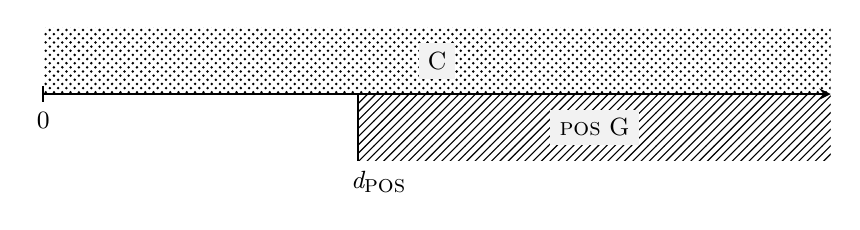
\begin{tikzpicture}		\label{Pos1}
\draw[-stealth,line width=0.8pt] (0,0) -- (10,0);
\draw[line width=0.8pt] (0cm,3pt) -- (0cm,-3pt) node[anchor=north] {\small 0};
\draw[line width=0.8pt] (4cm,0pt) -- (4cm,-24pt) node[anchor=north] {\small $\textit{d}_{\rlap{\textsc{pos}}}$};
\path[pattern=north east lines, line width=0pt] (10cm,0) -- (4cm,0) -- (4cm,-24pt) -- (10cm,-24pt);
\path[pattern=crosshatch dots, line width=0pt] (10cm,0) -- (0cm,0) -- (0cm,24pt) -- (10cm,24pt);
\node[fill=black!5] at (7cm,-12pt) {\small \textsc{pos} G};
\node[fill=black!5] at (5cm,12pt) {\small C};
\end{tikzpicture}
}

\ex Intensität eines mittels \textit{sehr} modifizierten Intensivausdrucks: \medskip

{
\centering
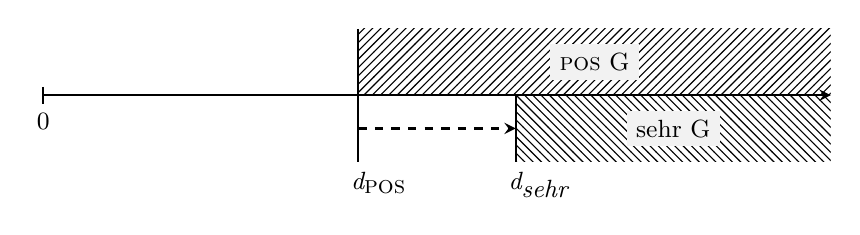
\begin{tikzpicture}   	\label{very1}
\draw[-stealth,line width=0.8pt] (0,0) -- (10,0);
\draw[line width=0.8pt] (0cm,3pt) -- (0cm,-3pt) node[anchor=north] {\small 0};
\draw[line width=0.8pt] (4cm,24pt) -- (4cm,-24pt) node[anchor=north] {\small $\textit{d}_{\rlap{\textsc{pos}}}$};
\draw[line width=0.8pt] (6cm,0pt) -- (6cm,-24pt) node[anchor=north] {\small $\textit{d}_{\rlap{\textit{sehr}}}$};
\draw[line width=0.8pt,dashed,-stealth] (4cm,-12pt) -- (6cm,-12pt);
\path[pattern=north east lines, line width=0pt] (10cm,0) -- (4cm,0) -- (4cm,24pt) -- (10.cm,24pt);
\path[pattern=north west lines, line width=0pt] (10cm,-24pt) -- (6cm,-24pt) -- (6cm,0pt) -- (10cm,0pt);
\node[fill=black!5] at (7cm,12pt) {\small \textsc{pos} G};
\node[fill=black!5] at (8cm,-12pt) {\small sehr G};
\end{tikzpicture}
}

\newpage
\ex  Intensität eines mittels \textit{mega} modifizierten Intensivausdrucks: \medskip


{
\centering
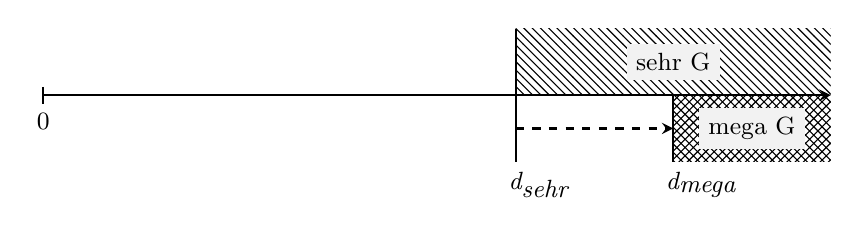
\begin{tikzpicture}
\draw[-stealth,line width=0.8pt] (0,0) -- (10,0);
\draw[line width=0.8pt] (0cm,3pt) -- (0cm,-3pt) node[anchor=north] {\small 0};
\draw[line width=0.8pt] (6cm,24pt) -- (6cm,-24pt) node[anchor=north] {\small $\textit{d}_{\rlap{\textit{sehr}}}$};
\draw[line width=0.8pt] (8cm,0pt) -- (8cm,-24pt) node[anchor=north] {\small $\textit{d}_{\rlap{\textit{mega}}}$};
\draw[line width=0.8pt,dashed,-stealth] (6cm,-12pt) -- (8cm,-12pt);
\path[pattern=north west lines, line width=0pt] (10cm,0pt) -- (6cm,0pt) -- (6cm,24pt) -- (10cm,24pt);
\path[pattern=crosshatch, line width=0pt] (10cm,0pt) -- (8cm,0pt) -- (8cm,-24pt) -- (10cm,-24pt);
\node[fill=black!5] at (8cm,12pt) {\small sehr G};
\node[fill=black!5] at (9cm,-12pt) {\small mega G};
\end{tikzpicture}
}
 \z
 \z

\noindent Mithilfe der Darstellung in \REF{gramo3} ist zu erkennen, dass das Verschieben auf der Skala bei \textit{mega} zu einem veränderten Begriffsumfang führt, da die bezeichnete Eigenschaft auf weniger Gegenstände zutrifft. Dem allgemeinen Verständnis von Expressivität folgend drückt der Satz in \REF{Te3} nicht bloß einen erhöhten Ausprägungsgrad der Aufregung aus, sondern er kommuniziert auch die persönliche Einstellung des Sprechers zum bezeichneten Sachverhalt \citep[vgl.][19]{Gutzmann.2019a}. Im obigen Beispiel ist z.\,B. denkbar, dass der Satz von Teds Trauzeugen Marshall geäußert wird, der Teds bester Freund ist und bereits in der gleichen Situation war, daher in einem besonders hohen Maße mit Bräutigam Ted mitfühlt. Abermals steigern ließe sich der Ausprägungsgrad durch Aneinanderreihung mehrerer expressiver Varianten. Somit gehen Sätze wie \textit{Ted ist super mega krass aufgeregt} mit einer besonderen Nachdrücklichkeit einher. Deskriptive Ausdrücke entziehen sich der Reihung dagegen vollkommen: \textit{\#Ted ist außerordentlich überaus sehr aufgeregt}. Bei ihnen kann eine Verstärkung des Ausprägungsgrades allenfalls durch Reduplikation erzielt werden: \textit{Ted ist sehr, sehr aufgeregt}.\footnote{Expressive Intensivierer funktionieren hinsichtlich Reduplikation natürlich analog: \textit{Ted ist mega, mega aufgeregt}.}

Die beiden anderen Charakteristika, die \citet[]{Gutzmann.2019a} im Zusammenhang mit Intensivierern hervorhebt, sind syntaktischer Natur. So stellt er fest, dass manche expressiven Intensivierer neben Adjektiven und Adverbien unter bestimmten Bedingungen auch adjazente Nomen modifizieren können, was mit deskriptiven Intensivierern wiederum komplett ausgeschlossen sei. Diese Behauptung untermalt er mit folgendem Beispiel:

\ea  \label{Schrott}
\ea Du hast eine \textbf{totale} Schrottkarre. \label{total}
\ex[*]{Du hast eine \textbf{sehr} Schrottkarre. \label{sehr}}
 \z
 \z
Laut \citet[20]{Gutzmann.2019a} klingt Satz \REF{total} für deutsche Muttersprachler:innen absolut natürlich, wohingegen die Modifikation des Nomens durch den deskriptiven Intensivierer \textit{sehr} in Satz \REF{sehr} nicht möglich ist. Im Falle adnominaler Intensivierung erhält der expressive Intensivierer die erforderliche Flexionsendung (\textit{total} + \textit{e}). Wie in Abschnitt \ref{Funktionsklasse} dargelegt, muss der Grad der durch das Nomen ausgedrückten Eigenschaft inhärent variabel, steigerbar und auf eine Skala abbildbar sein. In {Beispiel \REF{Schrott}} bedeutet dies, dass dem Nomen \textit{Schrottkarre} bzw. der Dimension `Mit Mängeln behaftetes Fahrzeug' eine Skala zugrunde gelegt wird, auf die die mit dem Gegenstand assoziierte Eigenschaft projiziert werden kann. {\citet[140ff.]{Gutzmann.2019a}} erläutert weiterhin, dass nicht alle expressiven Intensivierer gleichermaßen Nomen modifizieren können, was er vornehmlich auf deren Flektierbarkeit sowie die Zugehörigkeit zur \textit{total}-Gruppe, d.\,h. zu derjenigen semantischen Klasse zurückführt, die inhärent über einen hohen Intensivierungsgrad verfügen. Im gleichen Zug spricht {\citet[20]{Gutzmann.2019a}} deskriptiven Intensivierern wie \textit{sehr} die Verwendbarkeit in adnominaler Position vollständig ab. Dem stimme ich nur bedingt zu, lässt sich im Hinblick auf dieses Argument doch einwenden, dass das Problem ebenso wie bei den expressiven Intensivierern nicht an der Intensiviererklasse als solche, sondern an der Möglichkeit zur Flexion zu liegen scheint. So ist \textit{sehr} als unifunktionale Partikel grundsätzlich nicht flektierbar, weswegen es im Satz nicht adnominal auftreten kann. Anders sieht dies hingegen bei solchen deskriptiven Intensivierern aus, die als Polyseme neben dem Ursprungslexem vorkommen.

\ea  \label{Schrott3}
\ea Du hast eine \textbf{außerordentliche} Schrottkarre.
\ex Du hast eine \textbf{beträchtliche} Schrottkarre.
\ex Du hast eine \textbf{echte} Schrottkarre.
\ex Du hast eine \textbf{regelrechte} Schrottkarre.
\ex Du hast eine \textbf{richtige} Schrottkarre.
 \z
 \z
Alle in \REF{Schrott3} gelisteten deskriptiven Intensivierer stammen von polysemen Adjektiven oder Adverbien ab, die für gewöhnlich uneingeschränkt flektiert werden können. Als Intensivierer sind sie der Klassifikation von {\citet[408]{Breindl.2007}} zufolge als affirmative Grenzwert-Intensifikatoren anzusehen, die mit einem absoluten Endpunkt und ähnlich wie expressive Intensivierer inhärent mit einem hohen Intensivierungsgrad einhergehen. Anders als bei expressiven Intensivierern wie \textit{furchtbar} oder \textit{übel}, die gleichfalls von polysemen Adjektiven abstammen, überwiegt hier allerdings nicht die adjektivische Bedeutung. Stattdessen scheint durchaus die mit dem Nomen \textit{Schrottkarre} assoziierte Eigenschaft (nämlich ein mit Mängeln behaftetes Fahrzeug zu sein) verstärkt zu werden, was bedeutet, dass auch deskriptive Intensivierer prinzipiell adnominal modifizierend sein können. Dieser Punkt bleibt bei {\citet[]{Gutzmann.2019a}} jedoch gänzlich unberücksichtigt.

Der letzten Eigenschaft, die von \citet[20]{Gutzmann.2019a} beleuchtet wird, liegt die Beobachtung zugrunde, dass expressive Intensivierer bei adverbialem Gebrauch in einer DP-externen Position, d.\,h. vor dem Determinierer, stehen können (vgl. hierzu auch \citealt[121ff.]{Meinunger.2009} und \citealt[]{Schmidlin.2015}). Dies ist syntaktisch aus verschiedenen Gründen ungewöhnlich: Zum einen ist diese Position im Deutschen generell bloß für Adverbien wie \textit{vermutlich} oder nicht vorfeldfähige Modalpartikeln wie \textit{doch} vorgesehen {\citep[vgl.][184]{Schmidlin.2015}}. Zum anderen steht die Bewegung aus der DP heraus im Widerspruch zu dem, was in klassischen Grammatiken über die syntaktische Position von Intensivierern festgehalten ist: \glqq{}Sie stehen stets vor dem Ausdruck, auf dem sie operieren.\grqq{} (\citealt[56]{Zifonun.1997}). Wird ein expressiver Intensivierer der DP vorangestellt, so hat er eine modifizierende Funktion auf die gesamte DP. Die folgenden von {\citet[20]{Gutzmann.2019a}} angeführten Sätze zeigen ebendiesen Unterschied zwischen den beiden Klassen:

\ea   \label{dpex}
\ea Das ist \textbf{sau} das schnelle Auto. \label{sau2}
\ex Das ist \textbf{total} die Schrottkarre. \label{total2}
 \z
 \z

\ea   \label{dpex02}
\ea[*]{Das ist \textbf{sehr} das schnelle Auto. \label{sehr1}}
\ex[*]{Das ist \textbf{sehr} die Schrottkarre. \label{sehr2}}
 \z
 \z
Die beiden Sätze in Beispiel \REF{dpex} demonstrieren, dass die expressiven Intensivierer ebenso außerhalb der DP stehen können, ohne dass der Satz inakzeptabel ist. Dagegen können deskriptive Intensivierer wie \textit{sehr} nicht vor die DP positioniert werden, wie Beispiel \REF{dpex02} nahelegt. Diesen Umstand erklärt {\citet[16]{Os.1989}} unter Verweis auf \citet[22]{Abraham.1986} mit folgender Aussage: \glqq{}Diese beschränkte Platzierbarkeit ist selbstverständlich darauf zurückzuführen, daß \textit{sehr} nur Intensivierungspartikel ist - die Partikel ist voll grammatikalisiert \textelp{} und konventionalisiert\grqq{}. Während \textit{sehr} ausschließlich graduierende Funktion habe, sei die Polyfunktionalität von expressiven Intensivierern der Grund für die freie Beweglichkeit im Satz \citep[vgl.][16]{Os.1989}. In DP-externer Position bilden expressive Intensivierer zusammen mit der DP eine Konstituente, die nicht trennbar und lediglich als Ganzes verschiebbar ist, wie {\citet[144]{Gutzmann.2019a}} an folgenden beiden Sätzen demonstriert:

\ea   \label{dpex2}
\ea[*]{\textbf{Sau} hast du die coole Party verpasst.}
\ex[*]{Die coole Party hast du \textbf{sau} verpasst.}
 \z
 \z
Wie in Beispiel \REF{dpex2} zu sehen ist, werden die beiden Sätze durch das Auftrennen von expressivem Intensivierer und DP ungrammatisch; ein klares Indiz dafür, dass es sich um eine syntaktisch zusammengehörige Einheit handelt. \citet[155]{Gutzmann.2012} erläutern, dass die Wahl zwischen DP-interner und DP-externer Konstruktion nicht willkürlich ist, sondern im Wesentlichen vom verwendeten Determinierer abhängt. So lassen ausschließlich definite Artikel DP-externe Konstruktionen zu, wohingegen die Realisierung mit indefiniten Artikeln (genauso wie mit Demonstrativ- und Possessivpronomen oder Quantoren) hingegen ausgeschlossen ist {\citep[vgl.][155]{Gutzmann.2012}}.\footnote{\citet[146]{Gutzmann.2019a} weicht diese Beschränkung insoweit auf, als er anmerkt, dass sich in Bezug auf die Gebrauchspräferenzen prinzipiell zwei Gruppen ausmachen lassen: einerseits diejenigen, für die DP-externe Konstruktionen mit indefinitem Artikel überhaupt nicht infrage kommen, und andererseits solche, die diese durchaus akzeptabel finden. Ob diese Einschätzung empirischen Überprüfungen standhält, kann hier nicht beantwortet {werden.}} Die Idee dahinter wird an den Sätzen aus dem oben präsentierten Beispiel \REF{dpex} vorgeführt.

\ea
\ea[*]{Das ist \textbf{sau} ein schnelles Auto. \label{sau3}}
\ex[*]{Das ist \textbf{total} eine Schrottkarre. \label{total3}}
 \z
 \z
Die Erklärung, die \citet[159f.]{Gutzmann.2012} für die DP-externe Intensivierung anbieten, besteht grob skizziert in der Annahme zweier unterschiedlicher Positionen innerhalb der DP: Stehen die deskriptiven Intensivierer klassischerweise adjazent zum Adjektiv und somit tief innerhalb der DP (vgl. \REF{K1}), sei die Position von expressiven Intensivierern hingegen im Strukturbaum höher in der Nähe der linken Peripherie angesiedelt {(vgl. \REF{K2})}. Dadurch sei es möglich, sie aus der DP herauszubewegen und dem definiten Determinierer voranzustellen, wie die Konstituentenstrukturen nach \citet[160]{Gutzmann.2012} verbildlichen:

\ea
\ea[*]{[\textsubscript{QP} sehr\textsubscript{\textit{i}} [\textsubscript{DP} die [\textsubscript{NP} [\textsubscript{DegP} Deg\textsuperscript{0} [\textsubscript{QegP} \textit{t}\textsubscript{\textit{i}} [\textsubscript{AP} coole ] ] ] Party ] ] ]   \label{K1}}
\ex[]{ [\textsubscript{QP} sau\textsubscript{\textit{i}} [\textsubscript{DP} die [\textsubscript{NP} [\textsubscript{DegP} \textit{t}\textsubscript{\textit{i}} [\textsubscript{QegP} Qeg\textsuperscript{0} [\textsubscript{AP} coole ] ] ] Party ] ] ] \label{K2}}
 \z
 \z


\largerpage
\noindent In externer Position werden expressive Intensivierer direkt an die DP adjungiert und verschmelzen mit dem Artikel zu einer Konstituente. Infolgedessen sei die daraus resultierende Interpretation somit nicht \textit{sau} [\textit{die} [\textit{coole Party}]], sondern [\textit{sau die}] [\textit{coole Party}]. Die Einheit, bestehend aus expressivem Intensivierer und Definitartikel, bewirke letztlich die Modifikation der Gesamtphrase \citep[vgl.][160]{Gutzmann.2012}. Den Umstand, dass in erster Linie expressive Intensivierer vor die DP gestellt werden können, führt \citet[353]{Androutsopoulos.1998} auf deren Starktonigkeit zurück, die dafür sorge, dass das Gesagte prominenter wahrgenommen werde. Die dadurch erzielte Aufmerksamkeit stehe zudem im Einklang mit dem Ziel, das Sprecher durch Intensivierung erlangen wollen. Nichtsdestotrotz zeichne sich ein Wandel ab: Sei die DP-externe Konstruktion wohl zunächst auf starktonige definite Determinierer beschränkt gewesen, deute die inzwischen ebenfalls mögliche Kombination mit unbetontem Definitartikel (und gegebenenfalls auch Indefinitartikel, wie dialektale Alltagsbeobachtungen zu bedenken geben: \textit{Das war ganz ein schöner Ton.}) auf eine Abschwächung der vormaligen Beschränkung hin, durch die das Anwendungsspektrum der Herausbewegung breiter geworden sei {\citep[vgl.][353]{Androutsopoulos.1998}}.

Daneben weist die DP-externe Intensivierung ebenso semantische Besonderheiten auf. Obwohl die Konstruktion mehrheitlich mit definitem Determinierer auftritt, wird dieser inhaltlich jedoch wie ein indefiniter Determinierer verstanden \citep[vgl.][155f.]{Gutzmann.2012}. Dies bezeichnen \citet[]{Gutzmann.2012} als \glqq{}syntax-semantics mismatch\grqq{}. Demnach verwenden Sprecher eigenartigerweise den Definitartikel, um sich auf etwas Indefinites zu beziehen, wodurch dessen eigentliche referenzsemantische Funktion nicht zum Tragen kommt. So erläutert \citet[187]{Schmidlin.2015}, dass mithilfe des indefiniten Determinierers für gewöhnlich unbekannte Referenten in einen Diskurs eingeführt werden, die im weiteren Verlauf anaphorisch mittels Pronomen oder Definitartikel wieder aufgegriffen werden können: \textit{\textbf{Ein} Mann betritt die MacLaren's Bar. \textbf{Er} trägt einen grauen Smoking und heißt Barney. \textbf{Der} Mann geht zum Tresen und bestellt ein Bier}. In DP-externer Position ist die Bedeutung expressiver Intensivierer also mit einem \glqq{}Indefinitheitseffekt\grqq{} (\citealt[]{Wang.2007}) verknüpft, der in regulärer, d.\,h. DP-interner Position nicht vorkommt. Festzuhalten ist, dass das Resultat der Verschiebung des expressiven Intensivierers \textit{sau} aus Beispiel \REF{dpex} die Verschmelzung mit dem Definitartikel zu [\textit{sau das}] nach sich zieht. Das Endprodukt erhält wiederum eine neue, steigernde Bedeutung, die unterdessen weitgehend lexikalisiert und trotz des definiten Determinierers semantisch indefinit zu interpretieren ist {\citep[vgl.][162f.]{Gutzmann.2012}}.

Auch wenn die Überlegungen von \citet[]{Gutzmann.2012} durchaus nachvollziehbar sind und ich ihnen darin beipflichte, dass sich deskriptive Intensivierer heute im Standarddeutschen gänzlich der Extraposition entziehen, erscheint es dennoch fraglich, dies pauschal als Auswirkung von Expressivität zu generalisieren und auf alle Ausdrücke gleichermaßen zu beziehen. Meiner Ansicht nach ist die Sichtweise der Autor:innen in dem Sinne zu undifferenziert, dass rein intuitiv vielmehr graduelle Abstufungen hinsichtlich der Akzeptabilität in Erwägung zu ziehen sind. So kann der Argumentation von \citet[]{Gutzmann.2012} entgegengehalten werden, dass es einige expressive Intensivierer gibt, bspw. \textit{total} oder \textit{voll}, die in DP-externer Position im Allgemeinen konventionalisierter und daher unmarkierter sind. Dagegen sind andere in dieser Position markiert(er) bis hin zu gänzlich {inakzeptabel}:\footnote{Mit einem Fragezeichen (?) versehene Sätze sind zwar nicht stark markiert, jedoch für Muttersprachler:innen mutmaßlich nicht zur Gänze natürlich. Der Asterisk (*) symbolisiert hingegen die totale Inakzeptabilität des Satzes. Beides beruht auf subjektiver Einschätzung.}

\ea   \label{Haha}
\ea[]{ Das war total\,/\,voll das geile Konzert. 	\label{voll2}}
\ex[?]{Das war mega\,/\,super das geile Konzert. \label{hammer}}
\ex[?]{Das war absolut\,/\,hammer das geile Konzert. 	\label{mega2}}
\ex[*]{Das war arsch\,/\,scheiße das geile Konzert. \label{arsch2}}
\ex[*]{Das war furchtbar\,/\,schrecklich das geile Konzert. \label{furchtbar}}
 \z
 \z
Während \REF{voll2} für mich vollkommen natürlich klingt,\footnote{Ich verwende den Terminus \textit{Natürlichkeit} im Sinne von \citet[113]{Dressler.1989}, nach dem \textit{natürlich} für die unmarkierte Form eines Ausdrucks steht, deren Akzeptabilität von Muttersprachler:innen nicht infrage gestellt wird.} da [\textit{total} + DP] oder [\textit{voll} + DP] gängige Konstruktionen darstellen, finde ich {\REF{hammer} und \REF{mega2}} demgegenüber deutlich markierter. Genauso klingt meinem sprachlichen Empfinden nach auch der von \citet[20]{Gutzmann.2019a} angeführte Satz {aus \REF{sau2}} weniger akzeptabel. Dies weckt Zweifel daran, dass die Konstruktion {[\textit{sau} + DP]} in gleichem Maße etabliert ist wie Satz \REF{total2} bzw. [\textit{total} + DP]. Ferner demonstrieren die Intensivierer in \REF{arsch2} und \REF{furchtbar} die Notwendigkeit, die getroffene Generalisierung in mehreren Punkten einzuschränken. Interessanterweise berichtet \citet[266]{Becher.1907} darüber hinaus von seinerzeit möglicher Positionierung des deskriptiven Intensivierers \textit{sehr} vor den Artikel, die dem Muster mancher expressiver Intensivierer entspricht:
\glqq{}Das is sehr e guter Kerl\grqq{}. Dadurch liegt die Vermutung nahe, dass die Extraposition von Intensivierern eine Stufe im Grammatikalisierungsprozess darstellt: Lassen sich vergleichsweise neue Intensivierer wie \textit{mega} oder \textit{voll} problemlos der DP voranstellen, scheint dies mit älteren Intensivierern wie \textit{schrecklich} oder \textit{sehr} hingegen ausgeschlossen. Je weiter grammatikalisiert ein Intensivierer ist, desto inakzeptabler ist womöglich seine Extraposition. Dies würde bspw. erklären, aus welchen Gründen dieses Phänomen lediglich innerhalb der expressiven Intensiviererklasse anzutreffen ist, gilt diese doch als erheblich dynamischer als die deskriptive Intensiviererklasse. Nichtsdestotrotz muss auch expressiven Intensivierern unterstellt werden, dass nicht alle in gleicher Weise von Extraposition betroffen sind, wie sich in Beispiel \REF{Haha} beobachten lässt.\footnote{Vor diesem Hintergrund nennt \citet[95]{Renz.2020} Adjektive wie \textit{brutal} und \textit{pervers} sowie Adverbien wie \textit{echt} und \textit{wirklich} sowie \textit{dermaßen} und \textit{so}, die eine satzmodifizierende Funktion haben. Auch verweist er neben den bereits genannten einschlägigen Autor:innen auf \citet[]{Schlieben.1995}, \citet[236f.]{Pittner.2006} und {\citet[190]{Schmidlin.2015}}, die diese Beobachtung für eine Reihe weiterer Intensivierer gemacht haben.} Auch sollten zusätzlich zu den lexikalischen Eigenschaften der Ausdrücke die äußeren Rahmenbedingungen hinzugezogen werden. So ist zu erwarten, dass sich bei der DP-externen Intensivierung, ebenso wie bei den expressiven Intensivierern im Allgemeinen, regionale bzw. diatopische, soziolektale und möglicherweise auch prosodische Präferenzen zeigen. Dies bedarf zweifelsohne einer empirischen Überprüfung. Gleichwohl an dieser Stelle keine Erklärung für die Eigenart einzelner expressiver Intensivierer geboten wird, drängt sich dennoch die Frage auf, welche Bedingungen die DP-externe Positionierung begünstigen. Wie \citet[]{Gutzmann.2012} beschreiben, sind notwendige Voraussetzungen, dass die betreffende Teilmenge expressiv ist und gleichzeitig mit einem Definitartikel auftritt, der letztlich indefinit interpretiert wird. Die zunehmende Menge an expressiven Intensivierern, die DP-extern in Erscheinung treten können, ist nach {\citet[168]{Androutsopoulos.1999}} ein Indiz für einen Konventionalisierungsprozess, der das Anwendungsspektrum der Konstruktion sukzessive erweitert. Die Gründe, die die Extraposition konditionieren, sind bislang allerdings noch nicht ausreichend erforscht, weshalb empirische Untersuchungen vonnöten sind, um gesicherte Aussagen darüber treffen {zu können}.

Ergänzend sei eine weitere syntaktische Besonderheit herausgegriffen, die expressive Intensivierer von deskriptiven unterscheidet: So können erstere nicht in Form von elliptischen Kurzantworten, d.\,h. als Responsiv, gebraucht werden, wie \citet[159]{Gutzmann.2012} ebenfalls diskutieren. Dies wird in \REF{Responsiv} illustriert.

\ea   \label{Responsiv}
\ea Lily: \glqq{}Freust du dich auf Teds Hochzeit?\grqq{} 	\label{freu}
\ex Robin: \glqq{}Ja, sehr\,/\,total\,/\,ziemlich.\grqq{} \label{}	\label{freu1}
\ex Robin: \glqq{}?\,Ja, mega\footnote{Nach Ansicht von \citet[182]{Schmidlin.2015} ist \textit{mega} als Kurzantwort möglich, meines Erachtens ist es zwar leicht markiert, aber doch deutlich akzeptabler als die Konstruktionen in \REF{freu2}.}\,/\,übelst\,/\,voll.\grqq{}	\label{freu3}
\ex Robin: \glqq{}*\,Ja, krass\,/\,sau\,/\,super.\grqq{}	\label{freu2}
 \z
 \z
Es ist zu sehen, dass die deskriptiven Intensivierer in \REF{freu1} reibungslos als Satzäquivalente dienen können, wobei sie als Analepse zu Lilys Frage fungieren \citep[vgl.][56]{Zifonun.1997}. Dieser Rückbezug sei aufgrund der Polyfunktionalität von expressiven Intensivierern wie in \REF{freu2} in den meisten Fällen nicht ohne Weiteres möglich, wie \citet[159]{Gutzmann.2012} überdies argumentieren. Jedoch sind auch hier Abstufungen in der Akzeptabilität anzunehmen, sind die Intensivierer in \REF{freu3} dem Anschein nach doch weniger kritisch als die Intensivierer in \REF{freu2}. Verantwortlich hierfür ist laut {\citet[182]{Schmidlin.2015}} der lexikalische Status, handelt es sich bspw. bei \textit{voll} und \textit{übelst} um von Adjektiven abgeleiteten Partikeln. Diese seien im Unterschied zu Präfixoiden wie \textit{sau} oder \textit{super} dahingehend grundsätzlich weniger stark beschränkt, wodurch sie durchaus auch als kurze Antwort infrage kommen {\citep[vgl.][182]{Schmidlin.2015}}. Trotzdem scheint mir \textit{mega} ebenso weniger stark markiert zu sein als die in \REF{freu2} gelisteten Ausdrücke, was eventuell auf eine stärkere Usualisierung zurückzuführen ist.

\subsubsection{Zur Entwicklung von Intensivierern} \label{Entwicklung}
Aus der Definition des Terminus \textit{Steigerungspartikel} nach {\citet[650]{Bussmann.2002}}, gemäß derer ein fundamentales Merkmal das zahlreiche Vorkommen ist, leitet sich die übergeordnete Frage ab, welche Gründe es für den Variantenreichtum gibt. Sie erklärt, dass die inhärente Affektivität der Ausdrücke der Auslöser für die \glqq{}ungewöhnlich hohe Verschleißrate\grqq{} sei. Inwiefern diese Affektivität die Entstehung von neuen Intensivierern motiviert, ist Gegenstand dieses Abschnitts.

In der Literatur (vgl. u.\,a. \citealt[]{Keller.1990, Keller.1994}; \citealt[]{Kirschbaum.2002b}; \citealt[]{Keller.2003}) wird die Position vertreten, dass bei der Entstehung von Intensivierern eine unsichtbare Hand\footnote{Die Metapher der \glqq{}unsichtbaren Hand\grqq{} stammt ursprünglich von dem Ökonomen Adam Smith, der sie dazu benutzt, um wirtschaftliche Strukturen und Prozesse zu erklären \citep[vgl.][92]{Keller.1990}. Exemplarisch für ein solches \glqq{}Phänomen der dritten Art\grqq{} nennt {\citet[97]{Keller.1990}} das Entstehen von Verkehrsstaus, Trampelpfaden oder Kassenschlangen.} beteiligt ist. Darin wird Sprache bzw. Sprachwandel als ein \glqq{}Phänomen der dritten Art\grqq{} verstanden, das weder durch naturbezogene noch menschliche Faktoren bedingt sei. Stattdessen handele es sich um das Resultat intentionalen Verhaltens einer Vielzahl von Individuen, das nicht kontrolliert werden könne {\citep[vgl.][92]{Keller.1994}}. Demzufolge setzen ähnliche zielgerichtete, wenn auch unbeabsichtigte Handlungen zahlreicher Personen einen unaufhaltsamen Prozess in Gang. Angetrieben wird dieser nach Ansicht von \citet[]{Hauschild.1899} durch eine hohe Gebrauchsfrequenz, die dazu führt, dass sich Intensivierer sukzessive abnutzen und ihre expressive Wirkung verlieren: \glqq{}Das Verstärkungswörtchen \textelp{} ist dem Bedeutungsverluste ganz besonders ausgesetzt. Je häufiger ein solches Wort gebraucht wird, um so rascher wird es verbraucht.\grqq{} {(\citealt[2]{Hauschild.1899}}). Zudem finden sich Hinweise darauf, dass neben der Frequenz auch die Dauer des Gebrauchs eine zentrale Rolle für den Expressivitätsschwund spielt. Die Beobachtung, dass sich sprachliche Elemente nach und nach abschleifen und dadurch ihren kommunikativ-pragmatischen Effekt einbüßen, ist keineswegs neu und wird von {\citet[59]{Tobler.1868}} und {\citet[253]{Gabelentz.2016}} schon zu Beginn des letzten Jahrhunderts thematisiert:

\begin{quotation} \noindent Was erst neu und selten war, wird dann alltäglich, und damit verliert es an Kraft, verblasst, rückt schliesslich wohl gar in die Reihe jener abstracten Bestandtheile der Rede, die es hatte verbessernd und verstärkend ergänzen sollen, und die es am Ende wohl gar verdrängte und ersetzte.

 \hfill (\citealt[253]{Gabelentz.2016})  \end{quotation}
 

Um den Ausfall abgenutzter Formen zu kompensieren und als Sprecher auch weiterhin expressiv bleiben zu können, bedarf es laut {\citet[274]{Baumgarten.1908}} ständiger produktiver Innovation und Erweiterung des bestehenden Inventars. Der Kompensation liegt ein iterativer diachroner Prozess zugrunde, der mit neuen Ausdrücken immer wieder aufs Neue durchlaufen wird und sich bloß retrospektiv anhand des Resultats nachvollziehen lässt (vgl. u.\,a. \citealt[120]{Lipka.1981}; {\citealt[85]{Skommer.1992}}; {\citealt[71]{Blank.2001}}). Der Lebenszyklus beginnt für gewöhnlich mit einem syntaktischen Wandel, entwickeln sich Intensivierer doch vorrangig aus Adjektiven und somit Inhaltswörtern hin zu Funktionswörtern. Doch wie wird dieser anscheinend natürliche Erneuerungsprozess ausgelöst und welche Bedingungen müssen erfüllt sein, damit ein lexikalisches Element die Intensiviererrolle annehmen kann? Diesen Fragen wird nachfolgend auf den {Grund gegangen}.

Das Ziel dieses Abschnitts liegt darin, den Entstehungsprozess mithilfe beispielhaft verwendeter lexikalischer Stellvertreter zu umreißen. Die Ausgangslage bildet ein Ausdruck, den es meinem subjektiven Empfinden nach noch nicht lange in intensivierender Funktion gibt und bei dem eine solche Entwicklung denkbar ist, nämlich \textit{krass}. Bei dem entworfenen Szenario handelt es sich um ein hypothetisches Konstrukt, das mitnichten der tatsächlichen Genese der angeführten Intensivierer entspricht. Stattdessen dienen die Ausdrücke der Illustration des offenbar zeitlich {begrenzten Lebenszyklus}.

\subsubsubsection{Auslöser und Grundprinzipien}

Bei der Entstehung von Intensivierern handelt es sich um einen produktiven Bedeutungswandel, bei dem ein sprachlicher Ausdruck aus pragmatischen Gründen eine neue, grammatische Bedeutung erhält.\footnote{Grammatische Neu- oder Urschöpfungen, die vom Sprecher schlicht erfunden werden, kommen bei grammatischen Zeichen nicht vor. Diese seien auf existente lexikalische Zeichen beschränkt, wie {\citet[1254]{Lehmann.1995}} erklärt. Demnach bedienen sich Sprecher stets an bereits bestehendem Inventar, was im Einklang mit dem oben angeführten {Ökonomieprinzip steht}.} Die morphologische Repräsentation des konvergierten Intensivierers unterscheidet sich nicht von der des Ursprungslexems: So erhielt bspw. das Adjektiv \textit{schrecklich} durch Bedeutungsanreicherung eine neue, intensivierende Funktion. Aus der semantischen Innovation resultiert notwendig Polysemie, bei der Ursprungs- und Quelllexem als Varianten desselben Bedeutungsspektrums nebeneinander existieren. In diesem Zusammenhang spricht \citet[27]{Gevaudan.2007} von \glqq{}semantische[m] Neologismus\grqq{}, der durch unterschiedliche semantische Inhalte bei gleichzeitiger morphologischer Kontinuität gekennzeichnet sei.

Der Innovationsprozess ist üblicherweise dadurch motiviert, dass vorzugsweise ein qualitatives Adjektiv oder Nomen von einem einzelnen, meist jüngeren Sprecher zu einer Intensitätspartikel umfunktioniert wird. Die Motivation hierfür ist trivial: Durch sein individuelles, zweckrationales Vorgehen will der Sprecher maximalen kommunikativen Erfolg erzielen (vgl. {\citealt[92]{Keller.1994}}; \citealt[189ff.]{Kirschbaum.2002b}). Dies gelingt ihm am besten, indem er nicht auf gewöhnliches, vorhersehbares Material zurückgreift, sondern sich möglichst innovativ und aufsehenerregend ausdrückt. Der Anstoß für den Wandel liegt also im Verhalten des Einzelsprechers, der sein Umfeld durch einen Ausdruck mit höherer pragmatischer Schlagkraft zur Imitation anspornt. Wird der Intensivierer nun aus vergleichbaren Gründen von einer Vielzahl von Sprechern übernommen und mit steigender Frequenz verwendet, so führt dies sukzessive zur Verbreitung, d.\,h. Konventionalisierung und Lexikalisierung, der neuen grammatischen Funktion. Der Vorgang, bei dem ein Inhaltswort mit eigenständiger lexikalischer Bedeutung zu einem semantisch entleerten Funktionswort reanalysiert wird, entspricht laut \citet[2]{Heine.2002a} dem Grundprinzip der Grammatikalisierung. Im Zuge dessen besteht die Gefahr, dass Bestandteile der Grundbedeutung obsolet werden, was in der Literatur als \glqq{}semantic bleaching\grqq{} (\citealt[2]{Heine.2002a}) bezeichnet wird: Die Ausgangsbedeutung des Ausdrucks verblasst und ist für die Sprechergemeinschaft nicht länger transparent. Zurück bleibt nur noch die Gradbedeutung {\citep[vgl.][74f.]{Sahel.2013}}. Wie in Abschnitt \ref{Intensivierertypen} beschrieben, ist dies z.\,B. beim deskriptiven Intensivierer \textit{sehr} zu verzeichnen, aber auch das englische \textit{very} ist in diesem Kontext exemplarisch zu nennen.

\subsubsubsection{I. Ausgangspunkt}

Im Normalfall handelt es sich bei Intensivierern um hyperbolische, d.\,h. Normabweichung denotierende Ausdrücke mit stark positiver oder negativer Konnotation, die in der Regel als oftmals stilistisch markierte Synonyme neben neutralen, deskriptiven Intensivierern wie \textit{sehr} oder \textit{überaus} existieren. Mit der Verwendung eines neuen Ausdrucks kommt es zu einer Abweichung vom gegenwärtigen regulären Sprachgebrauch. Laut \citet[352]{Claudi.2006} trägt der Innovations- und Markiertheitsgrad des Neulings zur Verstärkung der durch das Bezugselement ausgesagten Eigenschaft bei. Der Entwicklungszyklus von Intensivierern wird im Folgenden am Beispiel von \textit{krass} skizziert.

Der Intensivierer \textit{krass} ist aufgrund seines Neuheitsgrades und der damit verbundenen expressiven Wirkung gegenwärtig insbesondere bei Jugendlichen sowie jüngeren Erwachsenen beliebt, da er es ermöglicht, die in Abschnitt \ref{Auslöser} erläuterten Nutzensfaktoren nach \citet[189ff.]{Kirschbaum.2002b} zufriedenstellend zu erfüllen. Das bedeutet, dass er zum einen ausdrucksstark genug ist, um dem Adressaten die subjektive Haltung des Sprechers unmissverständlich anzuzeigen. Zum anderen kann sich der Sprecher damit innerhalb einer gesellschaftlichen Gruppe sprachlich profilieren. Zudem trägt \textit{krass} als Intensivierer zum Ökonomieprinzip bei, da dessen Äußerung bloß geringe artikulatorische Kosten erfordert, wie das folgende {Beispiel aufzeigt}:

\ea  \label{konzert}
\ea[]{ Das Konzert am Wochenende war krass gut. \label{konzert1}}
\ex[\#]{Das Konzert am Wochenende war meiner Ansicht nach so gut, dass ich noch immer sehr aufgeregt bin. \label{konzert2}}
 \z
 \z
In Satz \REF{konzert1} drückt der Sprecher seine persönliche Einstellung zum beschriebenen Sachverhalt ohne Weiteres prägnant aus. Die deskriptive Paraphrasierung in Satz \REF{konzert2} ist hingegen nicht nur mit einem höheren kognitiven und motorischen Aufwand verbunden, sondern sie ist gemäß des Kriteriums der Nicht-Beschreibbarkeit nach \citet[]{Potts.2007a} überdies auch nicht in der Lage, die Bedeutung des Expressivsatzes exakt wiederzugeben. Dementsprechend kann der Sprecher mit der Verwendung von \textit{krass} den größtmöglichen verbalen Effekt bei gleichzeitig minimalen Artikulations- und Verarbeitungskosten erzielen: \glqq{}Wenn dich zwei Wege ans Ziel führen, und einer davon sowohl kürzer als auch sicherer ist, so solltest du diesen wählen.\grqq{} (\citealt[221]{Keller.1995}). Dies macht \textit{krass} meiner Meinung nach zum idealen Kandidaten für den Startpunkt des zu präzisierenden Entwicklungskreislaufs. Ausgangspunkt ist, wie oben angemerkt, der extravagante Gebrauch eines neuen, zur Intensitätspartikel umfunktionierten Ausdrucks durch einen einzelnen Sprecher.

\subsubsubsection{II. Pragmatische Inflation und Expressivitätsverlust}

Wenn der Sprecher merkt, dass er mit dem intensivierenden \textit{krass} mit Leichtigkeit das gewünschte Diskursziel erfüllen kann, resultiert dies unweigerlich darin, dass er es immer öfter verwendet. Mit zunehmendem Gebrauch routinisiert sich die kreative Neuschöpfung\footnote{Gemäß \citet[75]{Koch.1996} ist hier von einer \glqq{}pragmatisch-situativ verankerte[n] \textit{ad-hoc-Bildung}\grqq{} als Basis auszugehen, die infolge von Usualisierung und Lexikalisierung in den Wortschatz einer Gemeinschaft aufgenommen wird.} und hält durch Nachahmung vieler allmählich Einzug in den Wortschatz eines größeren Teils der Sprechergemeinschaft \citep[vgl.][171f.]{Androutsopoulos.1999}. Durch häufige Iteration wird ein Konventionalisierungsprozess in Gang gesetzt, der neben einer höheren Bekanntheit in der Lexikalisierung resultiert -- der Intensivierer wird folglich im mentalen Lexikon inventarisiert und dadurch in den Sprachgebrauch eingelagert, wodurch er vorhersehbarer wird. Mit der Einlagerung wird gleichsam eine usuelle Bedeutung etabliert, auf die Sprecher nach Bedarf zurückgreifen können. Je mehr der Ausdruck von der Sprechergemeinschaft angenommen, je länger und häufiger er gebraucht wird, desto stärker festigt er sich darin und entwickelt sich zu einem usualisierten, gewöhnlichen Ausdruck (vgl. \citealt[59]{Tobler.1868}; \citealt[1055]{Haspelmath.1999}; {\citealt[3]{Heine.2002a}}).

\citet[2]{Hauschild.1899} und \citet[1055]{Haspelmath.1999} schildern, dass die vermehrte, stereotype Verwendung von Ausdrücken zu Inflation und Abnutzung führt. In diesem Sinne ist davon auszugehen, dass das intensivierende \textit{krass} allmählich seine expressive Kraft verliert, wenn es zu häufig gebraucht wird.\footnote{Auch wenn der Fokus der folgenden Ausführungen auf der Frequenz als Ursache für Expressivitätsverlust liegt, gilt nach \citet[59]{Tobler.1868} Ähnliches für die Dauer des Gebrauchs.} Als Konsequenz davon kann der Sprecher das intendierte Diskursziel durch den Gebrauch von \textit{krass} irgendwann also nicht mehr erreichen:

\begin{quotation} \noindent [A] grammatical construction is initially used for a special communicative effect that gives a short-term advantage to the innovator \textelp{}, but as more and more people are trying to get their share of this advantage \textelp{}, the advantage disappears, and the system has undergone a change. \par \hfill (\citealt[1061]{Haspelmath.1999})  \end{quotation}

\noindent Aus diesem Grund wird der Sprecher von dessen Gebrauch künftig absehen und den Intensivierer allmählich durch neue, extravagantere Ausdrücke ersetzen: \glqq{}Ein häufig verwendeter Ausdruck verliert zwangsläufig seine Originalität und damit seine `Daseinsberechtigung'.\grqq{} {(\citealt[190f.]{Kirschbaum.2002b})}. Somit kommt es in dieser Phase oftmals zu einem Kampf miteinander konkurrierender Intensivierer, bei dem sich alte und neue Ausdrücke in Bezug auf ihren Gebrauch gegenüberstehen. Gleichwohl sich in der Literatur Belege für Ausdrücke finden, die mit dem Schwund der intensivierenden Funktion ebenso anderweitig aus dem Sprachgebrauch entfallen sind, z.\,B. \textit{bäumig}\footnote{Obwohl \textit{bäumig} in intensivierender Funktion aus dem Standarddeutschen komplett verschwunden ist, findet es sich dennoch in einigen schweizerdeutschen Dialekten in der Bedeutung von `großartig, toll' \citep[vgl.][18]{Bickel.2012}.} bzw. \textit{boomig}, \textit{gletscherhaft} oder \textit{pyramidal} (vgl. {\citealt[135]{Tobler.1868}}; {\citealt[7f.]{Mueller.1899}}; {\citealt[268]{Becher.1907}}), folgt daraus jedoch nicht notwendig, dass auch das polyseme Adjektiv als lexikalischer Ursprung {obsolet wird}.

\subsubsubsection{III. Semantische Innovation als Kompensationsstrategie}

Infolge der soeben erörterten Abnutzung ergibt sich laut {\citet[274]{Baumgarten.1908}} ein Bedarf an neuen sprachlichen Formen, die die ursprüngliche Expressivität mindestens in dem gleichen Maß ausdrücken. Demzufolge begibt sich der Sprecher auf die Suche nach neuen Ausdrücken, die er zur Intensivierung nutzen kann. Nach {\citet[95]{Dahl.2001}} ist es nämlich ökonomischer, einen abgenutzten Ausdruck zu ersetzen, als ihn mühsam wiederzubeleben. Ersatz findet sich für gewöhnlich in bestehendem Material, oftmals in wertenden Adjektiven, die durch Grammatikalisierung der Zielfunktion gemäß reanalysiert werden. Vor diesem Hintergrund erklärt \citet[188]{Kirschbaum.2002b}, dass es praktikabler sei, \glqq{}einen bereits vorhandenen sprachlichen Ausdruck in einer abweichenden Interpretation zu verwenden als einen neuen Ausdruck zu `erfinden'.\grqq{} Dieser Vorgang kommt einer Verdrängung des alten, verbrauchten Intensivierers durch einen neuen, pragmatisch ausdrucksstärkeren gleich. So ist bspw. vorstellbar, dass das bis dato vermutlich ausschließlich als Adjektiv vorkommende \textit{toxisch}\footnote{Meinem Wissen nach gibt es das Adjektiv \textit{toxisch} bislang nicht in intensivierender Funktion, es erscheint mir aber aufgrund seiner Bedeutung sowie der damit verbundenen konnotativen Markiertheit allerdings dafür geeignet.} zum Intensivierer umfunktioniert wird und der Sprecher dadurch wieder imstande ist, das gewünschte kommunikative Ziel zu erreichen. Für den abgeschliffenen Intensivierer \textit{krass} bedeutet die Verdrängung, dass er als Verlierer aus dem Konkurrenzkampf hervorgeht und in der Folge zukünftig seltener oder allenfalls mit rein skalarer Bedeutung verwendet wird.

\subsubsubsection{IV. Konventionalisierung und Lexikalisierung}

\citet[85f.]{Heine.2002b} zufolge handelt es sich bei der Entstehung von grammatischen Bedeutungen um einen mehrstufigen Prozess, bei dem der Ausdruck in seiner Grundbedeutung den Ausgangspunkt, d.\,h. Stufe I, bildet.\footnote{Ein vergleichbares Entwicklungsszenario beschreibt \citet[187ff.]{Kirschbaum.2002b}.} Dieser Prozess wird im Folgenden als Grundlage verwendet, um die Entwicklungsstufen von Intensivierern aufzuzeigen. Auf Stufe II, den \glqq{}bridging contexts\grqq{} (\citealt[5]{Evans.1998}), wird einem Lexem über die eigentliche Funktion hinaus die Rolle als Intensivierer zugewiesen. Dies geschieht, indem die ursprüngliche Bedeutung mittels Inferenz auf die Ziel- bzw. Gradbedeutung übertragen wird -- es kommt also zu einer Bedeutungserweiterung {\citep[vgl.][83]{Paul.1880}}. Die Ausgangsbedeutung bleibt in der Phase der Übertragung unberührt und vordergründig. Auf Stufe III, den \glqq{}switch contexts\grqq{}, rückt laut \citet[86]{Heine.2002b} die Zielbedeutung in den Fokus, wohingegen die Ausgangsbedeutung aufgrund semantischer Konflikte zwar sukzessive im Hintergrund verschwindet, jedoch noch immer auf die Zielbedeutung einwirkt. Daher kommt es in dieser Phase zur Divergenz von Ausgangs- und Zielbedeutung \citep[vgl.][86]{Heine.2002b}. Auf {Stufe IV} sind die Konventionalisierung und Lexikalisierung der Gradbedeutung zu verorten, die fortan gänzlich unabhängig von der Ausgangsbedeutung ablaufen. Durch die Ablösung von der Ausgangsbedeutung lässt sich die neue, vordergründige Zielbedeutung auch in solchen Kontexten verwenden, die keinerlei Nähe zur Ausgangsbedeutung aufweisen (vgl. \citealt[86]{Heine.2002b}). In dieser Phase festigt sich der Intensivierer allmählich innerhalb der Sprechergruppe, sodass er einen eigenen Lexikoneintrag erhält. Gleichzeitig expandiert sein Anwendungsbereich, was bedeutet, dass sich die Menge der Gegenstände oder Sachverhalte, auf die der Intensivierer referiert, d.\,h. seine Denotation, vergrößert. In Kombination mit der damit verbundenen Delexikalisierung bzw. Desemantisierung ermöglicht es die Kollokationsausweitung, dass von nun an gemischte Kombinationen mit unterschiedlicher Polarität auftreten können, ohne dass der sprachliche Ausdruck markiert ist. In diesem Zusammenhang nennt {\citet[400]{Breindl.2007}} die Kombinationen \textit{höchst niedrig} oder \textit{äußerst nah}, aber auch \textit{voll leer} ist ein hervorragendes Beispiel für eine Intensivierung mithilfe eines dem Adjektiv semantisch entgegengesetzten Operators, was im Allgemeinen als Zeichen vollständiger Grammatikalisierung betrachtet wird (vgl. {\citealt[61]{Tobler.1868}}; {\citealt[118]{Biedermann.1969}}; \citealt[194f.]{Kirschbaum.2002b}).\footnote{Auch \citet[7]{Hauschild.1899} und \citet[268]{Becher.1907} machen diese Beobachtung. Letzterer nennt als Beispiele solcher \glqq{}sinnlos[en] oder gar widersinnig[en]\grqq{} Verbindungen \textit{rießig klein} und \textit{eklig fein}.}

\subsubsubsection{V. Zurück zur Ausgangslage}

Mit der Habitualisierung eines neuen Intensivierers wie \textit{toxisch}, dem Zurückdrängen der Ausgangsbedeutung und der Ausweitung des Anwendungsbereichs schließt sich der Kreis, den die Entwicklung durchläuft. Somit sind wir wieder am Ausgangspunkt angelangt, an dem der Kreislauf mit einem neuen Intensivierer wie \textit{toxisch} von vorne beginnen kann. {\citet[92]{Keller.1994}} hebt als entscheidenden Aspekt hervor, dass es sich um ein unvermeidbares, quasi naturgegebenes Ergebnis handelt, das durch ähnliches Verhalten einer Vielzahl von Menschen verursacht wird. Dies geschehe grundsätzlich unwillentlich: \glqq{}Speakers have many goals when they use language, but changing the linguistic system is not one of them.\grqq{} ({\citealt[70]{Croft.2000}}). Statt Sprachwandel auszulösen, geht es Sprechern also vielmehr darum, die gewünschten kommunikativen Absichten zu erreichen (vgl. die Expressivitätsmaximen nach \citealt[]{Kirschbaum.2002b} in Abschnitt {\REF{Auslöser}}).

\subsubsubsection{Resümee}

Das aufgezeigte Entwicklungsszenario verdeutlicht die in der theoretischen Literatur vorherrschende Annahme, dass sich Intensivierer durch Routinisierung und damit verbundener häufiger Verwendung abnutzen und ihre expressive Wirkung verlieren, was wiederum negative Auswirkungen auf deren Existenz hat, sofern sie nicht als rein skalare Intensivierer beibehalten werden (vgl. u.\,a. \citealt[2]{Hauschild.1899}; \citealt[253]{Gabelentz.2016}; \citealt[274]{Baumgarten.1908}; \citealt[171f.]{Androutsopoulos.1999};; \citealt[1055]{Haspelmath.1999}; \citealt[3]{Heine.2002a}; \citealt[190f.]{Kirschbaum.2002b};; \citealt[74f.]{Sahel.2013}). Als Folge davon entstehen ständig neue Ausdrücke, mit denen sich Sprecher auch weiterhin als ausdrucksstark, innovativ und originell darstellen können:

\begin{quotation}
\noindent A newly coined expression will still carry the flavour of originality and strikingness. As soon as it is used repeatedly and imitated by more speakers in more contexts, this originality and strikingness will of course get lost, or `fade away', and {leave} the expression as a neutral part of language. \par \hfill (\citealt[30f.]{Eckardt.2006})   \end{quotation}

Die Grundidee des soeben beschriebenen diachronen Entwicklungsprozesses von Intensivierern wird nachfolgend angelehnt an die Ausführungen von \citet[285]{Tagliamonte.2005} in Abbildung \ref{Entwick} schematisch dargestellt. Im Flussdiagramm stellen die durchgehenden Verbindungspfeile das direkte, beobachtbare Resultat der vorangegangenen Stufe dar, während die abzweigenden gestrichelten Pfeile die Vorbedingung repräsentieren, die erfüllt sein muss, damit eine Intensitätspartikel auf die nächsthöhere Stufe gehoben werden kann.


\begin{figure}

\tikzstyle{decision} = [diamond, draw, fill=blue!20,
    text width=4.5em, text badly centered, node distance=1cm, inner sep=0pt]
\tikzstyle{block} = [rectangle, draw,
    text width=10em, text centered, rounded corners, minimum height=4em]
\tikzstyle{line} = [draw, -latex']
\tikzstyle{cloud} = [draw, rectangle, node distance=4.43cm,
    minimum height=3.6em]
\tikzstyle{every node}=[font=\small]

\begin{tikzpicture}[node distance = 2cm, auto]
    \node [block] (lex) {Innovativer Gebrauch durch Einzelsprecher};
    \node [cloud, right of=lex] (emph) {\parbox{2cm}{Okkasionelle\\Bedeutung}};
    \node [block, below of=lex, node distance=2.2cm](freq) {Nachahmung durch zahlreiche Sprecher};
    \node [cloud, left of=freq] (wide) {\parbox{1.8cm}{Konventio-\\nalisierung}};
    \node [block, below of=freq, node distance=2.2cm](lost) {Lexikalisierung};
     \node [cloud, right of=lost] (usu) {\parbox{1.8cm}{Usuelle\\Bedeutung}};
    \node [block, below of=lost, node distance=2.2cm](abnutz) {Abnutzung durch frequenten Gebrauch};
    \node [cloud, left of=abnutz] (konk) {\parbox{2cm}{Lexikalische\\Konkurrenz}};
    \node [block, below of=abnutz, node distance=2.2cm](sterb) {Rückgang des nun veralteten Ausdrucks};
    
   	\path [line] (lex) -- (freq);
    \path [line] (freq) -- (lost);
    \path [line] (lost) -- (abnutz);
    \path [line] (abnutz) -- (sterb);
    \path [line,dashed] (lex) -- (emph);
    \path [line,dashed] (emph) |- (freq);
    \path [line,dashed] (freq) -- (wide);
      \path [line,dashed] (lost) -- (usu);
      \path [line,dashed] (usu) |- (abnutz);
    \path [line,dashed] (wide) |- (lost);
    \path [line,dashed] (abnutz) -- (konk);
    \path [line,dashed] (konk) |- (sterb); 
\end{tikzpicture}

\caption[Flussdiagramm zur zyklischen Entwicklung von Intensivierern] {Flussdiagramm zur zyklischen Entwicklung von Intensivierern (Eigene Darstellung in Anlehnung an \citealt[285]{Tagliamonte.2005}).} \label{Entwick}
\end{figure}

\subsubsection{Semantische Herkunft von Intensivierern} \label{Quellensemantisch}
Vor dem Hintergrund des in Abschnitt \ref{Entwicklung} beschriebenen Entstehungsprozesses leitet sich die Frage ab, welcher semantischen Natur sprachliche Ausdrücke sein müssen, um die Rolle des Intensivierers einnehmen zu können. In diesem Kontext gelangt \citet[229]{Pittner.1989} zu dem Schluss, dass \glqq{}Steigerungsglieder häufig homonym zu Wörtern mit hohem expressiven Gehalt sind\grqq{}, die aufgrund ihrer bisweilen derben Konnotation nahezu geschaffen für die verstärkende Funktion seien. Zusätzlich zu Wahrheitsbeteuerungen schreiben \citet[50,\,302]{Heine.2002a} sowie \citet[192f.]{Stratton.2020b} vor allem negativen Ausdrücken die Eigenschaft zu, als Intensitätspartikeln reanalysiert zu werden. Wie die bisherigen Ausführungen bereits gezeigt haben, greift dies deutlich zu kurz, entstammen viele gegenwärtige Intensivierer doch aus verschiedenen anderen Domänen.\footnote{Vgl. u.\,a. \citet[]{Hauschild.1899} und \citet[]{Becher.1907} für die meines Wissens ältesten Klassifikationen sowie \citet[]{Suscinskij.1985}, Kirschbaum (2002a,\,b), \citet[]{Nuebling.2004a} und {\citet[]{Breindl.2007}} für neuere Einordnungen.} Um die einleitende Frage zu beantworten, zielt dieser Abschnitt darauf ab, die fruchtbarsten semantischen Herkunftsbereiche nach \citet[]{Claudi.2006} vorzustellen, die Intensivierer feinkörnig nach ihren inhärenten semantischen Merkmalen einteilt.\footnote{Weitere Einteilungen finden sich bspw. in \citet[]{Biedermann.1969} und \citet[]{Os.1989}.} Zur vertiefenden Auseinandersetzung sei auf \citet[]{Laitenberger.2016} verwiesen.

\subsubsubsection{Die einträglichsten Quellbereiche}   \par   \label{Quelleneintraeglich}
Wie \citet[353]{Claudi.2006} erklärt, stammen Intensitätspartikeln meist von polysemen Adjektiven ab, was ein Indiz dafür ist, dass die oben beschriebene Polysemie den Normalfall darstellt. Ein weitaus geringerer Teil lässt sich auf ebenfalls polyseme Nomen wie \textit{Mord}, \textit{Sau} oder \textit{Stroh} zurückführen, die in der Regel als Kompositionsglieder in Erscheinung treten (vgl. {\citealt[299]{Pittner.1989}}; {\citealt[140]{Gutzmann.2019a}}). \citet[]{Claudi.2006} beruft sich ausschließlich auf Ausdrücke mit adjektivischem Ursprung und klassifiziert zahlreiche im Gegenwartsdeutschen vorkommende Intensivierer umfassend nach Wortgruppen. Weil diese Klassifikation den Eindruck macht, weitgehend erschöpfend zu sein, orientieren sich sowohl die Kategorisierung der Quellbereiche als auch deren Einteilung vornehmlich an ihren Ausführungen. Beides wird anschließend überblicksartig wiedergegeben.

\subsubsubsubsection{Quantität und Größe/Umfang}

Diese Klasse beinhaltet all diejenigen Intensivierer, deren semantischer Ursprung auf eine messbare räumliche Dimension zurückgeht, ganz gleich, ob die Größe, das Gewicht oder das Volumen betreffend. Als Beispiele nennt \citet[354]{Claudi.2006} u.\,a. \textit{ganz}, \textit{giga}, \textit{komplett}, \textit{mega}, \textit{schwer}, \textit{total}, \textit{völlig} und \textit{voll}. Die Beliebtheit der beiden aus dem Griechischen stammenden Ausdrücke \textit{giga} und \textit{mega} führt sie auf die heutige digitale, computerzentrierte Zeit zurück, in der Begriffe wie \textit{Gigabyte} oder \textit{Megahertz} alltäglich sind. Da die Semantik der Intensivierer laut \citet[354]{Claudi.2006} neutral ist, richtet sich deren Polarität zur Gänze nach dem modifizierten Adjektiv oder muss aus dem Kontext hergeleitet werden. In der Folge können sie gleichermaßen positiv wie negativ intensivierend verwendet werden. Durch ihre Aufwärtsgerichtetheit geben die Intensivierer in erster Linie an, dass die im Satz bezeichnete Eigenschaft über ein bestimmtes Durchschnittsmaß hinausgeht: \glqq{}[T]hey simply add an emphasized `plus' to the respective adjective meaning\grqq{} (\citealt[354]{Claudi.2006}).

\subsubsubsubsection{Unwirklichkeit}

In diese Gruppe ordnet \citet[355]{Claudi.2006} all diejenigen Ausdrücke, die das Zutreffen eines Sachverhalts in irgendeiner Weise infrage stellen bzw. ihn als übernatürlich oder nicht mit Worten beschreibbar deklarieren. Exemplarisch finden sich hier \textit{fabelhaft}, \textit{märchenhaft}, \textit{phänomenal}, \textit{sagenhaft}, \textit{traumhaft}, \textit{unbeschreiblich}, \textit{unfassbar}, \textit{unglaublich} und \textit{unvorstellbar}. Auch deren Bedeutung ist nach {\citet[355]{Claudi.2006}} häufig neutral, steht bei dieser Gruppe doch primär die Überschreitung des Rationalen im Vordergrund. Als Ausnahme hebt sie \textit{fabelhaft}, \textit{märchenhaft}, \textit{phänomenal} und \textit{traumhaft} hervor: Da deren inhärent positive Bedeutung noch vordergründig ist, können sie bloß Adjektive der gleichen Polarität intensivieren. Die Modifikation negativer Adjektive ziehe statt Verstärkung hingegen vielmehr eine nicht intendierte modale Interpretation nach sich: \textit{traumhaft gut} vs. \textit{\#traumhaft schlecht} \citep[vgl.][356]{Claudi.2006}.

\subsubsubsubsection{Furcht und Abscheu}

Wie der Name schon andeutet, enthält diese Gruppe bei \citet[356]{Claudi.2006} ausnahmslos Ausdrücke mit klar negativem Ursprung. Hierzu gehören u.\,a. \textit{arg}, \textit{entsetzlich}, \textit{furchtbar}, \textit{grauenhaft}, \textit{schrecklich}, \textit{ungeheuer}, \textit{unheimlich} und \textit{unsäglich}, die bspw. \citet[165ff.]{Biedermann.1969} und \citet[]{Hentschel.1998b} eingehend diskutieren. Diese \glqq{}Gradadverbien des Schreckens\grqq{} (\citealt[53]{Laitenberger.2016}) gelten vor allem durch die negative Konnotation und die damit verbundene Signalwirkung als prädestiniert für die Rolle des Intensivierers. Gleichwohl zahlreiche dieser Intensivierer vermutlich weitgehend delexikalisiert sind, z.\,B. \textit{furchtbar} und \textit{schrecklich}, sind einige davon hinsichtlich ihres Gebrauchs stärker restringiert. So ist ein aus zwei negativen Elementen bestehender Intensivausdruck wie \textit{entsetzlich schlecht} in Bezug auf Intensivierung vollkommen unproblematisch, wohingegen ein in puncto Polarität gemischter Intensivausdruck wie \textit{\#entsetzlich gut} nicht möglich ist \citep[vgl.][356]{Claudi.2006}. Dies ist ein Indiz dafür, dass die Ursprungsbedeutung von \textit{entsetzlich} noch nicht ausgebleicht genug ist, was sich \citet[284]{Tagliamonte.2005} zufolge durch eine eingeschränkte Anwendbarkeit äußert. Intensivierer mit fortgeschrittenerem Delexikalisierungsgrad können dagegen auch positive Adjektive modifizieren: \textit{furchtbar schlecht} {vs. \textit{furchtbar gut}}.

\subsubsubsubsection{Kraft und Gewalt}

Die nächste Gruppe setzt sich bei \citet[357]{Claudi.2006} aus Ausdrücken zusammen, die hauptsächlich für Kraft und Gewalt stehen, demnach qua Semantik physische Stärke oder Macht denotieren: bspw. \textit{ätzend}, \textit{brutal}, \textit{gewaltig}, \textit{knall-}, \textit{mächtig}, \textit{sehr}, \textit{überwältigend} und \textit{umwerfend}. Viele davon sind negativ konnotiert, sie können häufig aber dennoch zur Intensivierung positiver Adjektive gebraucht werden. Ausnahmen finden sich mit \textit{überwältigend} und \textit{umwerfend}, die inhärent mit einer positiven Bedeutung einhergehen. In Bezug auf die semantisch neutralen Intensivierer \textit{gewaltig}, \textit{knall-} und \textit{mächtig} bespricht \citet[357]{Claudi.2006}, dass deren Interpretation vorrangig durch den Gebrauchskontext erfolgt. Interessanterweise befindet sich in dieser Klasse ebenso ein Intensivierer mit opaker Semantik, nämlich \textit{sehr}, dessen Ausgangsbedeutung komplett verschwunden und für Sprecher und Adressat nicht mehr wahrnehmbar ist (vgl. auch Abschnitt \ref{Intensivierertypen}). Nichtsdestotrotz weist die Etymologie des Ausdrucks zweifelsfrei auf einen negativen semantischen Ursprung hin (vgl. {\citealt[1270]{Pfeifer.1995}}; \citealt[357]{Claudi.2006}).

\subsubsubsubsection{Wert und Wahrheit}

Die Intensivierer \textit{ausgemacht}, \textit{echt}, \textit{fürwahr}, \textit{richtig}, \textit{wahrhaft(ig)}, \textit{wahrlich} und \textit{wirklich} bilden bei \citet[357]{Claudi.2006} die Gruppe, die sich vorwiegend durch Wahrheitsbeteuerungen auszeichnet.\footnote{Ein:e anonyme:r Gutachter:in weist darauf hin, dass Adjektive aus dem damit verwandten Bereich `Angemessenheit und Anstand' mit Ausdrücken wie \textit{anständig}, \textit{ordentlich} und \textit{richtig} oft erst zu Modaladverbien und anschließend zu Intensivierern reanalysiert werden. Beispiele dafür finden sich sprachübergreifend: Englisch: \textit{proper} (Adj.) -- \textit{That was proper cool.} (Int.) \citep[vgl.][206]{Stratton.2021}, Deutsch: \textit{richtig} (Adj.) -- \textit{Er hat das richtig gemacht.} (Adv.) -- \textit{Das war richtig cool.} (Int.) \citep[vgl.][186]{Stratton.2020b}, Norwegisch: \textit{ordentlig} (Adj.) `ordentlich' -- \textit{Det var ordentlig dekorert.} (Adv.) `Das war ordentlich dekoriert.' -- \textit{Det var ordentlig stillig.} (Int.) `Es war sehr still.' \citep[vgl.][411]{Stratton.2022}, Niederländisch: \textit{behoorlijk} (Adj.) `ordentlich' -- \textit{Het was behoorlijk schoon.} (Int.) `Es war ganz sauber.' {\citep[vgl.][411]{Stratton.2022}}.} Wie eingangs dargelegt, stellen auch \citet[302]{Heine.2002a} diese Gruppe gesondert heraus. {\citet[109]{Os.1989}} bezeichnet solche Ausdrücke als \glqq{}propositional attitudes\grqq{}. Diese seien hauptsächlich propositionsbestätigend, insofern \glqq{}ein Sprecher mittels dieser Adverbien seine Aussage bekräftigt, {\textbf{seine}} Wahrheit, Aufrichtigkeit, Informiertheit usw. beteuert.\grqq{} (\citealt[85]{Os.1989}). {\citet[8f.]{Pittner.2006}} erklären, dass hier nicht immer eindeutig zu erkennen ist, ob der Ausdruck tatsächlich zur Steigerung des Adjektivs dient oder er lediglich die Aussage in Gestalt eines Satzadverbs als wahr hinstellt. Nach Auffassung der Autorinnen wird diese Funktionsambiguität durch die syntaktischen Position des Ausdrucks hervorgerufen, die in beiden Fällen die gleiche ist. Die Intensivierer dieser Gruppe können allesamt gleichfalls für positive wie auch negative Kontexte verwendet werden, was \citet[358]{Claudi.2006} auf deren Ursprungsbedeutung zurückführt: \glqq{}[T]heir basic meaning is the assurance that something is really what it seems to be, i.e. a statement that is neutral in
terms of good or bad\grqq{}.

\subsubsubsubsection{Mentale Störungen}

Eine weitere Klasse bilden bei {\citet[358]{Claudi.2006}} diejenigen Ausdrücke, die im Allgemeinen psychische Zustände und Erkrankungen denotieren. Zu diesen gehören u.\,a. \textit{bescheuert}, \textit{idiotisch}, \textit{irre}, \textit{irrsinnig}, \textit{rasend} und \textit{wahnsinnig}, die, genauso wie viele der zuvor genannten Intensivierer, von einem negativen Adjektiv abstammen und über eine offenkundig negative Semantik verfügen. Dadurch ist es wenig überraschend, dass sie die Intensiviererrolle angenommen haben, ist die Normalität doch nun einmal weniger aufsehenerregend als das von der Norm Abweichende. Dass diese Klasse durch ein reichhaltiges Inventar gekennzeichnet ist, hat schon \citet[275]{Bach.1950} sieben Dekaden zuvor für Dialekte erkannt: \glqq{}Die Mda [= Mundart] hat also dort die größte Anzahl von Ausdrükken, wo es sich um die Benennung der negativen Verstandeseigenschaften des Menschen handelt.\grqq{} Ungeachtet der konnotativen Markiertheit des Ursprungslexems lassen sich die Partikeln problemlos für die Intensivierung sowohl negativer als auch positiver Adjektive verwenden, wie \citet[358]{Claudi.2006} berichtet. Auch hier deutet die freie Kookkurrenz auf einen fortgeschrittenen Delexikalisierungsgrad hin, infolge dessen sich der Anwendungsbereich von Intensivierern für gewöhnlich auf semantisch gegenläufige Prädikate ausdehnt \citep[vgl.][284]{Tagliamonte.2005}. {\citet[358]{Claudi.2006}} ergänzt ferner, dass die Ausdrücke \textit{irre} und \textit{wahnsinnig} in prädikativer Verwendung positiv konnotiert sind: \textit{Das Lied ist der Wahnsinn!}

\subsubsubsubsection{Einzigartigkeit}

Die Mitglieder dieser Klasse fallen durch ihren singulären, beispiellosen Charakter auf. Dabei geben sie im Wesentlichen an, dass ihr Bezugselement im Hinblick auf das bezeichnete Merkmal aus einer Menge heraussticht \citep[vgl.][358]{Claudi.2006}. Als Beispiele hierfür nennt {\citet[358]{Claudi.2006}} die Ausdrücke \textit{absolut}, \textit{ausgenommen}, \textit{besonders}, \textit{einmalig}, \textit{nur}, \textit{selten} und \textit{ungewöhnlich}. Vor diesem Hintergrund erläutert sie, dass die Intensivierer gleichermaßen positiv wie negativ verstärkend sein können, was ihrer Ansicht nach deren semantischen Neutralität geschuldet ist \citep[vgl.][358]{Claudi.2006}.

\subsubsubsubsection{Grenz- oder Extrempositionen}

Die Intensivierer \textit{extrem}, \textit{galaktisch}, \textit{hoch}, \textit{hyper}, \textit{kosmisch}, \textit{super}, \textit{top} und \textit{ultra} lassen sich der Klassifikation von \citet[359]{Claudi.2006} zufolge in die Gruppe derjenigen Ausdrücke einordnen, die qua Semantik einen maximal entfernten Punkt denotieren, der eine Art Endpunkt oder Schwellenwert darstellt. Auffallend ist, dass diese Gruppe mit \textit{hyper}, \textit{super}, \textit{top} und \textit{ultra} gleich mehrere Lexeme enthält, die griechischen oder lateinischen Lehneinfluss aufweisen und sich ihrem etymologischen Ursprung nach auf einen bestimmten, oben gelegenen Referenzpunkt beziehen. Dies lässt die Vermutung zu, dass ihre Bedeutung einen inhärent steigernden Bestandteil aufweist, der sie zum Intensivierer qualifiziert. {\citet[359]{Claudi.2006}} unterstreicht außerdem, dass einige der Lehnwörter trotz neutraler Semantik im Deutschen positiv konnotiert sind. Dies ist bspw. am prädikativen Gebrauch von \textit{super} oder \textit{top} zu sehen: \textit{Marshalls Hochzeitsrede war super}. Daneben ist laut \citet[359]{Claudi.2006} auch die Bedeutung von \textit{hoch} als durchweg positiv zu betrachten, ist gemäß der traditionellen Metapherntheorie nach {\citet[14ff.]{Lakoff.1980}} alles Aufwärtsgerichtete doch positiv und erstrebenswert, wohingegen alles Abwärtsgerichtete gemeinhin mit Negativem in Verbindung steht. Zusätzlich befinden sich mit \textit{kosmisch} und \textit{galaktisch} in dieser Gruppe zwei Ausdrücke, die mit dem Weltraum zusammenhängen und die per se einen starken Bezug zu Höhe und räumlicher Ausdehnung anzeigen {\citep[vgl.][359]{Claudi.2006}}.

\subsubsubsubsection{Religion}

Diese Gruppe ist durch die Nähe zu Gott und Glaube motiviert und zerfällt bei \citet[359]{Claudi.2006} in \textit{göttlich}, \textit{himmlisch}, \textit{höllisch}, \textit{teuflisch}, \textit{verdammt} und \textit{verflucht}. Da Intensivierer ebenso wie Tabu- und Schimpfwörter häufig aus sensiblen Bereichen (z.\,B. aus dem krankheitsbezogenen oder skatologischen Bereich) stammen, gelten diese Ausdrücke als die optimalen Kandidaten, um einer Äußerung Nachdrücklichkeit zu verleihen {\citep[vgl.][189]{Kirschbaum.2002b}}. Vor diesem Hintergrund erläutert {\citet[83]{Klara.2009}}, dass solche Intensivierer im Mittelhochdeutschen vor allem durch die \glqq{}hohe Tabuisierung von Kirche und Glauben\grqq{} bedingt gewesen seien. Die Kookkurrenzmöglichkeiten betreffend erwähnt {\citet[359]{Claudi.2006}}, dass \textit{himmlisch} und \textit{göttlich} ausschließlich in positiven Kontexten auftreten, während die anderen Ausdrücke trotz der negativen Bedeutung ihres Ursprungslexems für die Verstärkung positiver wie auch negativer Adjektive verwendet werden können. Abgesehen von dem Hinweis auf eine ebenfalls fortgeschrittene Delexikalisierung ist ein Bezug zur \glqq{}schrecklichen\grqq{} Intensivierung zu erkennen: Die Ausdrücke \textit{verdammt} und \textit{verflucht} können im Deutschen bspw. interjektionell gebraucht werden, um u.\,a. Überraschung oder Verärgerung auszudrücken. Weitere Beispiele für Intensivierer aus dem religiösen Bereich finden sich auch in regionalen Sprachvarietäten.\footnote{Regionale Varietäten und Dialekte gelten ohnehin als produktiver, wenn es um expressive Innovationen geht (vgl. u.\,a. \citealt[60]{Tobler.1868}; \citealt[2]{Hauschild.1899}; \citealt[266]{Hauschild.1929}; \citealt[293]{Bach.1950}; {\citealt[32ff.]{Henzen.1954}}; {\citealt[90]{Klara.2009}}). Dieser Umstand liegt mutmaßlich an der für Sprachvarietäten typischen mündlichkeitsnahen Ausdrucksweise, die nach {\citet[89]{Koch.1996}} als Triebfeder für Expressivität gilt.} So verfügt das Bairische z.\,B. über den Ausdruck \textit{sakrisch}, der sich von Sakrament ableitet und ebenfalls zur Verstärkung gebraucht wird: \textit{Die Stimmung bei der Hochzeitsfeier war {sakrisch gut}}.

\subsubsubsubsection{Tierbegriffe}

Die Gruppe der Tierbegriffe wird bei \citet[360]{Claudi.2006} durch \textit{animalisch}, \textit{bestialisch}, \textit{säuisch}, \textit{saumäßig} und \textit{tierisch} repräsentiert und umfasst somit Ausdrücke, deren denotative Bedeutung klar erkennbar ist. Die semantische Transparenz ist offenbar auch der Grund dafür, wieso manche dieser heute abwertend verwendeten Ausdrücke im Deutschen Schimpfwortcharakter haben und sich metaphorisch auf Menschen beziehen lassen: \textit{Du dumme Sau}. Die heutige pejorative Bedeutung von \textit{sau} scheint jedoch nicht immer die vorherrschende gewesen zu sein: Wie {\citet[270]{Becher.1907}} erklärt, wurde das Schwein ehemals als heilig angesehen und daher verehrt,\footnote{Vgl. diesbezüglich bspw. \citet[]{Symbol.online} [letzter Aufruf: 10.08.2025].} weshalb die Ausdrücke \textit{Schwein} und \textit{Sau} in der Vergangenheit als Beteuerungsschwüre eingesetzt worden seien. Dies lässt vermuten, dass sich beim intensivierenden \textit{sau} ein Bedeutungswandel vollzogen hat, der im Gegensatz zu dem steht, was sein heutiger Schimpfwortcharakter erwarten lässt.\footnote{Das Schimpfwort \textit{Sau} wie in \textit{Du dumme Sau} existiert nach Angaben von \citet[1168]{Pfeifer.1995} seit dem Mittelhochdeutschen.} Im Kontext der Tierbegriffe nimmt \citet[360]{Claudi.2006} an, dass die Intensivierung vorwiegend durch einen Kontrast zwischen Mensch und Tier bzw. Zivilisation und Natur erlangt wird, bei dem das Tier durch unkontrollier- und unzähmbares Instinktverhalten auffällt. In der Folge gehen die meisten dieser Intensivierer gegenwärtig mit einer negativen Konnotation einher, die sich aufgrund ihrer pragmatischen Stärke ideal zur Intensivierung eignet -- ganz gleich, ob positiv oder negativ. Als Ausnahme hebt \citet[360]{Claudi.2006} \textit{animalisch} hervor, das seine negative Bedeutungskomponente ihres Erachtens unterdessen gänzlich verloren hat.

\subsubsubsubsection{Sonstige Quellen}

Schließlich führt \citet[360]{Claudi.2006} eine gemischte Klasse an, die all diejenigen Ausdrücke umfasst, die keiner der bisher genannten Gruppen zugeordnet werden können und sich auf unterschiedliche semantische Domänen zurückführen lassen. Hierzu gehören u.\,a. \textit{ausgesprochen}, \textit{entschieden}, \textit{gar}, \textit{herzlich}, \textit{schön}, \textit{sowas von}, \textit{verschärft}, \textit{verboten} und \textit{zu}, die zumeist sowohl positive als auch negative Adjektive intensivieren können. Die Ausdrücke \textit{verschärft} und \textit{verboten} zeichnen sich dabei durch die negative Bedeutung des Ursprungslexems aus. Nichtsdestotrotz können sie infolge von Delexikalisierung positiv wie negativ intensivierend sein \citep[vgl.][361]{Claudi.2006}. Zusätzlich stellt {\citet[361]{Claudi.2006}} \textit{herzlich} und \textit{schön} heraus, deren Adjektivbedeutung zwar grundsätzlich im Positiven verankert ist, die als Intensivierer allerdings vielmehr ironisch und deswegen negativ interpretiert werden: \textit{schöner Mann} vs. \textit{schön dumm}.

\subsubsubsection{Resümee}

\noindent Zusammengefasst zeigt die von \citet[]{Claudi.2006} vorgenommene Gruppierung, dass den meisten der gegenwärtig im Deutschen verwendeten Intensitätspartikeln metonymische oder metaphorische Muster zugrunde liegen und sie üblicherweise aus den verschiedensten semantischen Herkunftsbereichen stammen.\footnote{Vgl. diesbezüglich auch \citet[]{Kirschbaum.2002b, Kirschbaum.2002a}.} Die reanalysierten Ausdrücke wurden sukzessive grammatikalisiert und dadurch zu Funktionswörtern, wobei deren lexikalischer Ursprung dann entweder transparent geblieben (z.\,B. \textit{sau}) oder verblasst (z.\,B. \textit{sehr}) ist. Das Ursprungslexem eines Intensivierers muss nicht zwangsläufig nativ sein, sind einige Ausdrücke doch aus anderen Sprachen wie dem Griechischen oder Lateinischen entlehnt (bspw. \textit{mega}, \textit{super} und \textit{ultra}). Diese sind zuweilen aufgrund der Möglichkeit der interjektionellen oder prädikativen Verwendung des Herkunftslexems im Deutschen positiv konnotiert (bspw. \textit{wahnsinnig}), wodurch sie in intensivierender Funktion völlig frei kookkurrieren können. Auffällig ist, dass viele Intensivierer mit starken, aufwühlenden Emotionen oder Verhaltens- bzw. Charaktereigenschaften verbunden sind, die häufig negativer Natur sind. Dies steht im Einklang mit der in der Literatur (u.\,a.
{\citealt[165ff.]{Biedermann.1969}}; \citealt[]{Hentschel.1998b}) vertretenen Auffassung, dass zusätzlich zu dimensionalen vor allem negative Ausdrücke für die Intensiviererrolle prädestiniert sind: \glqq{}Denn besondere Expressivität lässt sich hervorragend durch Tabubruch zum Ausdruck bringen.\grqq{} ({\citealt[2]{Keller.2003}}). Daneben eignen sich auch positiv konnotierte Ausdrücke zur Intensivierung: Wörter wie \textit{krass}, \textit{mega}, \textit{super} oder \textit{top} können sowohl als positiv bewertende Adjektive als auch als Intensivierer fungieren {\citep[vgl.][]{Stratton.2022b}}. Des Weiteren eignen sich auch all diejenigen Ausdrücke zur Intensivierung, die Normabweichungen und somit etwas Unerwartetes oder Unvorhergesehenes denotieren, was per se bemerkenswerter als der Standard ist. Daneben ist oftmals eine Kontrastrelation wie Mensch\,--\,Tier, Mensch\,--\,Gott oder Wirklichkeit\,--\,Unwirklichkeit vordergründig, um nur einige der von {\citet[161]{Claudi.2006}} aufgeführten Vergleiche zu nennen.

Das nachfolgende \chapref{Korpus} stellt den ersten Empirieteil dar. Darin wird eine korpuslinguistische Analyse vorgestellt, die für ausgewählte expressive Intensivierer des Gegenwartsdeutschen (n = 16) durchgeführt wurde, mit dem Ziel deren synchrone und diachrone Häufigkeitsverteilungen zu ermitteln. Durch dieses Vorgehen wird erstmals einigen in der Literatur vorherrschenden Annahmen empirisch nachgegangen und erste Rückschlüsse auf die Rolle der Expressivität gezogen. Die quantitativen Ergebnisse der Korpusanalyse sowie die daraus abgeleiteten Implikationen und Mutmaßungen bilden daraufhin die Untersuchungsgrundlage des in {\chapref{Experiment0}} beginnenden experimentellen Teils dieses Buchs.




		%(4.135) Sie ist --- einsam.




%

\chapter{{Korpusstudie}} \label{Korpus}

In diesem Kapitel wird die Korpusanalyse präsentiert, die durchgeführt wurde, um eine Stichprobe an Intensitätspartikeln quantitativ einzuordnen.\footnote{Auszüge dieses Kapitels wurden in \citet[]{Schmidt.2022} veröffentlicht.} Wie in Abschnitt \ref{Funktionsklasse} erläutert, wird in der theoretischen Literatur die Position vertreten, dass Intensivierer eine Verschiebung von Graden auf einer Skala bewirken, wodurch dem jeweiligen Intensivausdruck eine stärkere Intensität und somit eine höhere Skalenposition zukommt. Der Unterschied zwischen deskriptiven und expressiven Intensivierern liegt darin, dass letztere mutmaßlich nicht nur skalierend sind, sondern auch die persönliche Einstellung des Sprechers zur geäußerten Sachlage ausdrücken (vgl. \citealt[315]{Lang.1983}; \citealt[57]{Ortner.2014}). Das Ziel dieser Untersuchung ist es, auf Grundlage eines Zeitschriftenkorpus die Frequenzverläufe verschiedener expressiver Intensivierer des Gegenwartsdeutschen (n = 16) über einen Zeitraum von rund 70 Jahren zu erfassen. Dadurch wird ermittelt, wie sich die Intensiviererklassen synchron und diachron quantitativ in einem schriftsprachlichen Kontext verhalten. Mithilfe der Ergebnisse können erste Rückschlüsse auf die Expressivität der Ausdrücke gezogen und Annahmen für weiterführende experimentelle Untersuchungen abgeleitet werden.

\section{Theoretischer Rahmen und Forschungshypothesen} \label{Forschungshypothesen-Korpus}

Wie einleitend geschildert, basiert die Untersuchung auf der Beobachtung, dass es im Deutschen eine Vielzahl von Intensivierern gibt. Dies wirft die Frage auf, welche Gründe es für den Variantenreichtum gibt. In diesem Kontext wird in der Literatur traditionell die These vertreten, dass diese Partikeln einem schnellen und unabdingbaren Wandel unterliegen (vgl. \citealt[2]{Hauschild.1899}; \citealt[267]{Becher.1907}; \citealt[274]{Baumgarten.1908}; \citealt[126f.]{Biedermann.1969};; \citealt[18]{Bolinger.1972}; \citealt[216f.]{Keller.1995};; \citealt[257]{Ito.2003}).\footnote{Neben dieser Erklärung gibt es in der soziolinguistischen Literatur auch soziale Ansätze zur Erklärung der Variation, indizieren Intensivierer doch auch soziale Bedeutung. So liefert der von einem Sprecher gewählte Ausdruck indirekt auch Informationen über Herkunft, Alter oder Geschlecht der Person. Auch wenn der Schwerpunkt dieses Buches nicht auf den sozialen Faktoren liegt, die zur Variation von Intensivierern beitragen, ist die soziale Dimension dennoch eng mit dem Phänomen der Intensivierungsvariation verknüpft.} Ihre Veränderlichkeit lässt sich laut \citet[189ff.]{Kirschbaum.2002b} primär auf das Streben nach Expressivität und Originalität zurückführen, durch das der Sprecher die größtmögliche kommunikative Wirkung beim Adressaten erzielen möchte: \glqq{}Wer in bestimmten Gruppen besonders expressive Ausdrücke verwendet, `kommt gut an'\grqq{} (\citealt[3]{Keller.2003}). Ist die Annahme, dass Entwicklungen von Intensivierern schnell vonstatten gehen und daher leicht nachzuvollziehen sind, faktisch gültig, so ist davon auszugehen, dass sie die ideale Basis für diachrone Korpusanalysen bieten.

Der Hauptantrieb für den Wandel des lexikalischen Inventars wird im Allgemeinen in zu hoher Frequenz gesehen, die ursächlich für den schnellen Verschleiß expressiver Ausdrücke sei und letztlich dazu führe, dass die intendierte Wirkung nachlasse: \glqq{}[W]eil jeder gerne imponieren möchte, werden solche Ausdrücke häufig verwendet; und wenn sie häufig verwendet werden, verlieren sie ihren expressiven `Pfiff'.\grqq{} (\citealt[3]{Keller.2003}). Mit anderen Worten: Je häufiger ein Intensivierer gebraucht wird, desto vorhersehbarer und weniger originell ist er. Dies wirkt sich in der Konsequenz auf seine Expressivität aus, die nach Ansicht von \citet[2]{Hauschild.1899} unweigerlich schwindet. Dadurch wird laut \citet[274]{Baumgarten.1908} neuen, expressiveren Ausdrücken der Weg in die Intensiviererrolle geebnet.\footnote{Als Beispiel für einen quantitativ rückläufigen Intensivierer führt \citet[10f.]{Hauschild.1899} \textit{wunder} an, das bereits im Althochdeutschen existierte, im Mittelhochdeutschen inflationär und seinerzeit nur noch selten gebraucht worden sei. Heute findet man \textit{wunder} bloß noch als Präfixoid in festen Konstruktionen wie bspw. \textit{wunderschön} (vgl. auch \citealt[228]{Pittner.1989}).}
Diese Gedankenfolge bildet den Ausgangspunkt dieser explorativen Korpusstudie, die den Entwicklungsgang von Intensivierern über die Zeit untersucht. Dadurch wird die Gültigkeit der folgenden häufig vertretenen, jedoch nicht empirisch abgesicherten Hypothesen überprüft:

\begin{itemize}
\item[\textbf{\textsc{H1}}] Eine hochfrequente Verwendung von Intensivierern führt unweigerlich zum Verlust ihrer Expressivität.

\item[\textbf{\textsc{H2}}] Der Expressivitätsverlust geht mit einem Bedarf an neuen Ausdrücken einher, mit denen sich Sprecher auch weiterhin als expressiv, innovativ und originell darstellen können.
\end{itemize}

\noindent Dabei lässt vor allem die Hypothese H1 Raum für Spekulation. In der Literatur wird gemeinhin als unkontrovers betrachtet, dass ein übermäßiger Gebrauch von expressiven Ausdrücken in unerwünschter Abnutzung und unvermeidlichem Expressivitätsverlust resultiert. Was die Hypothese nach meinem Verständnis allerdings ebenso zu beinhalten scheint, ist der Faktor Zeit. So ist anzunehmen, dass sich der Expressivitätsstatus eines Intensivierers nicht abrupt von expressiv zu nicht-expressiv verändert, sondern einem graduellen Wandel unterliegt. Dabei spielt vermutlich inhärent auch die Fortdauer seines Gebrauchs eine zentrale Rolle -- ein Aspekt, der meines Wissens bisher nicht berücksichtigt wurde. Dennoch hebt schon \citet[]{Tobler.1868} den Einfluss von Zeit wie folgt hervor:

\begin{singlespace*}
\begin{quotation} \noindent Im lauf der zeit versinkt dann die qualitative grundlage der bedeutung des ersten wortes immer mehr, und es bleibt blo\textlongs s gleichsam ein quantitativer niederschlag derselben, ein allgemeiner begriff von steigerung des zweiten durch das erste als seinen exponenten. \hfill (\citealt[59]{Tobler.1868}) \\ \end{quotation}
\end{singlespace*}

\noindent Abgesehen von der Verwendungshäufigkeit kommt also auch ein zweiter Parameter als Triebkraft für Expressivitätsverlust infrage, nämlich die Zeit. Um dem gerecht zu werden, wird die Hypothese H1 gemäß der soeben dargelegten Faktoren Frequenz und Zeit folgendermaßen spezifiziert: 

\begin{itemize} 
\setlength{\itemindent}{1cm}
\item[\textbf{\textsc{H1-Freq}}] Eine hochfrequente Verwendung von Intensivierern führt zu einer pragmatischen Abnutzung und demzufolge sukzessive zum Verlust von Expressivität. 

\item[\textbf{\textsc{H1-Temp}}] Eine persistente Verwendung von Intensivierern führt zu einer pragmatischen Abnutzung und demzufolge sukzessive zum Verlust von Expressivität. 
\end{itemize}

Da mittels einer frequenzbasierten Korpusuntersuchung lediglich das diachrone Vorkommen von Ausdrücken in einer Textsammlung erhoben wird, erlauben die ermittelten Daten naturgemäß keine Aussagen über den Expressivitätsgrad der Intensivierer. Nichtsdestotrotz liefern sie erste Informationen über die Rolle von Frequenz und Persistenz und können als Spiegelbild des potenziellen Expressivitätsverlusts dienen. Die longitudinale Entwicklung wird daher als erster Hinweis auf den Expressivitätsgrad eines jeden Intensivierers herangezogen. Im Hinblick auf die Hypothese H1 wird im Sinne der in Abschnitt \ref{Auslöser} beschriebenen Expressivitätsmaximen nach \citet[]{Kirschbaum.2002b} erwartet, dass die Frequenz eines neuen expressiven Intensivierers zunächst ansteigt, da er bei Sprechern aufgrund seiner bemerkenswerten Wirkung beliebt ist, er mit der Zeit und durch übermäßigen Gebrauch allerdings an Expressivität einbüßt. Dadurch wird er im weiteren Zeitverlauf entweder seltener (bspw. \textit{wunder})\footnote{In diesem Zusammenhang betont \citet[52]{Gevaudan.2007}, dass lexikalisierte Ausdrücke ohnehin nicht notwendigerweise persistent seien, sondern \glqq{}immer wieder gebraucht werden [müssen], sonst verfallen sie. \textelp{} Wenn die Verwendungshäufigkeit für ein Wort abnimmt, bis sie unter eine bestimmte Schwelle fällt, führt das zu lexikalischem Schwund.\grqq{}} oder mit rein skalierender Funktion (bspw. \textit{sehr}) verwendet. Letzteres hält \citet[12]{Hauschild.1899} zum intensivierenden \textit{blut} wie in \textit{blutjung} fest, das sich etwa im 17. Jahrhundert etabliert hätte, später jedoch seinen semantischen Gehalt verloren habe und infolgedessen \glqq{}nur noch als Verstärkungswörtchen gefühlt\grqq{} worden sei. Die Frequenzabnahme eines Ausdrucks wird mutmaßlich von einer Zunahme eines anderen, expressiveren Intensivierers begleitet. Durch den neuen Intensivierer können Sprecher den Verlust eines abgenutzten Ausdrucks kompensieren und auch zukünftig expressiv bleiben. Diese Vermutung geht auf \citet[]{Baumgarten.1908} zurück, der sich über Steigerungskomposita wie \textit{blitzblank} wie folgt äußert: \glqq{}So entstehen \textelp{} Wörter, an denen das Empfindungsleben in höchstem Maße beteiligt ist, die aber auch hier und da wieder verblassen, durch neue ersetzt oder in derselben Weise doppelt und dreifach gesteigert werden.\grqq{} (\citealt[274]{Baumgarten.1908}). Bezüglich der Hypothese H2 wird also erwartet, dass innerhalb des Untersuchungszeitraums neue expressive Intensivierer auftreten,\footnote{\textit{Untersuchungszeitraum} meint hier und im Folgenden die Zeitspanne, über die sich das Korpus erstreckt, und nicht den Zeitraum, in dem die Korpusanalyse durchgeführt wurde.} die ein Indiz für einen tatsächlich bestehenden Bedarf an neuen Ausdrücken sind und deren Gebrauchsfrequenz, im Einklang mit H1, ebenso vorerst zunimmt. Ein Zutreffen von H2 würde sich folglich in Form von neuen Ausdrücken niederschlagen, die sich erst im Laufe der Jahre erstmals in intensivierender Funktion im Korpus nachweisen lassen.

\largerpage
Zusammengenommen liegt das Ziel der Untersuchung darin, die bis dato als unzweifelhaft erachteten Hypothesen erstmals empirisch zu überprüfen, um stichhaltige Aussagen über deren Gültigkeit zu machen. Die erste stammt von \citet[2]{Hauschild.1899},\footnote{In der Literatur wird an dieser Stelle meist auf \citet[126f.]{Biedermann.1969}, \citet[99]{Suscinskij.1985} oder \citet[2]{Keller.2003} verwiesen. Dessen ungeachtet ist \citet[2]{Hauschild.1899}, soweit mir bekannt, der Erste, der die große Varianz von Intensitätsausdrücken bzw. Verstärkungskomposita auf die Frequenz als kausale Ursache zurückführt.} der anmerkt, dass Intensivierer zwangsläufig ihren expressiven Charakter verlieren. Diesen Verlust sehen er und andere Autor:innen hauptsächlich mit der Häufigkeit des Gebrauchs assoziiert: \glqq{}Frequenz ist der natürliche Feind von Expressivität.\grqq{} (\citealt[2]{Keller.2003}). Wie \citet[59]{Tobler.1868} und \citet[253]{Gabelentz.2016} beschreiben, hat neben der Frequenz eventuell auch die Dauer des Gebrauchs einen entscheidenden Einfluss auf die Expressivität. Die damit verbundene Abnutzung setze einen nicht-intendierten innovativen Wandel in Gange, der sich nach Auffassung von \citet[274]{Baumgarten.1908} durch neue Ausdrücke bemerkbar macht.\footnote{Wie schon \citet[]{Hauschild.1899} findet auch \citet[]{Baumgarten.1908} in neueren Arbeiten keine Erwähnung, sodass diesbezüglich im Allgemeinen auf Autor:innen wie z.\,B. \citet[18]{Bolinger.1972}, \citet[99]{Suscinskij.1985} oder \citet[391]{Tagliamonte.2008} Bezug genommen wird. Weil \citet[274]{Baumgarten.1908} sich dem Phänomen erheblich früher widmet, beziehe ich mich in diesem Buch folgerichtig auf ihn.} Diese ermöglichen Sprechern, die Expressivität trotz des Wegfalls altgedienter Formen beizubehalten, was zugleich die zweite der zu testenden Hypothesen ist.

\section{Methodisches Vorgehen} \label{Durchführung}

Die empirische Grundlage bildet eine korpuslinguistische Analyse von synchronen und diachronen Häufigkeitsverteilungen ausgewählter Intensivierer des Gegenwartsdeutschen. Durch dieses Vorgehen können mögliche Wandelprozesse, die sich im (in dieser Untersuchung schriftlichen) Sprachgebrauch abzeichnen, sichtbar und interpretierbar gemacht werden. Dabei besteht die Möglichkeit, dass Veränderungen in der Schriftsprache Rückschlüsse auf die gesprochene Sprache zulassen. So ist vorstellbar, dass der schriftliche Sprachgebrauch mitunter vom mündlichen Sprachgebrauch beeinflusst ist -- jedenfalls sofern es stilistisch der jeweiligen Textsorte entspricht. Wenn es die Textsorte gestattet, kann der schriftliche Sprachgebrauch gewissermaßen als Abbild des mündlichen Sprachgebrauchs betrachtet werden \citep[vgl.][]{Koch.1996,Koch.2007}.\footnote{Nichtsdestotrotz wird ausdrücklich hervorgehoben, dass es sich hierbei um schriftliche und nicht um gesprochene Daten handelt.} Zudem erlaubt die quantitative Einordnung der untersuchten Ausdrücke erste Mutmaßungen in Bezug auf die Rolle der Expressivität sowie den zu überprüfenden Expressivitätsverlust.

Korpusstudien haben im Vergleich zu Experimenten den Vorteil, dass durch beträchtliche Textsammlungen authentische, d.\,h. natürlichsprachliche Daten, zur %quantitativen und qualitativen
Analyse herangezogen werden können. Diese sind in elektronischer Form im Netz größtenteils frei zugänglich und bestenfalls bereits digital aufbereitet. Da Intensitätspartikeln dem Anschein nach zu schnellem Wandel neigen (vgl. \citealt[257]{Ito.2003}; \citealt[281]{Tagliamonte.2005}), bieten sie eine hervorragende Grundlage für Korpusanalysen, mithilfe derer synchrone und diachrone Häufigkeitsverteilungen ermittelt und Annahmen über die Rolle der Expressivität abgeleitet werden können. Die dadurch gewonnenen Daten können außerdem als Basis für weiterführende experimentelle Untersuchungen dienen.

\subsection{Belegkorpus}
Das als Stichprobe herangezogene Untersuchungskorpus wurde über das Deutsche Referenzkorpus [\textsc{DeReKo}] aus dem \textit{W\,-\,Archiv der geschriebenen Sprache} bzw. \textit{W\,-\,öffentlich} durch das Webinterface der Korpusmanagement- und Recherchesoftware \textsc{COSMAS II} (Version 2.3.5)\footnote{\citet[]{COSMAS.2020}: \textit{https://cosmas2.ids-mannheim.de/cosmas2-web/} \mbox{[letzter Aufruf: 25.02.2020]}.} extrahiert \citep[vgl.][]{Kupietz.2010}. Das \textsc{DeReKo} enthält über 350 elektronische Korpora geschriebener Sprache mit mehr als 42 Milliarden Textwörtern (Stand: 06.02.2018) und wird vom Leibniz-Institut für Deutsche Sprache in Mannheim (\citealt[]{IDS.2018}) kostenfrei bereitgestellt. Dessen Grundlage bilden alle systematisch konzipierten und öffentlich zugänglichen Textkorpora des W-Archivs (mit Neuakquisitionen), die allesamt morphosyntaktisch annotiert sind, insgesamt etwa 32 Millionen deutschsprachige Texte mit neun Milliarden Wortformen umfassen und somit vermutlich hinreichend repräsentative Belege für linguistische Analysen bereithalten. Das zurate gezogene \textit{W\,-\,Archiv der geschriebenen Sprache} setzt sich vornehmlich aus Zeitungs- bzw. Zeitschriftentexten, aber auch Protokollen aus Parlamentsdebatten sowie Beiträgen aus Diskussionsforen zusammen. Auf dieser Grundlage wurde ein eigenes virtuelles Untersuchungskorpus definiert, das alle Texte der über das \textsc{DeReKo} zur Verfügung gestellten digitalen Ausgaben der überregionalen, wöchentlich erscheinenden Zeitschriften \textsc{Der Spiegel}\footnote{Streng genommen handelt es sich beim \textsc{Spiegel} um ein Nachrichtenmagazin; er wird im Kontext dieser Untersuchung jedoch gemeinsam mit der \textsc{Zeit} als Zeitschrift bezeichnet.} im Zeitraum von Januar 1950 bis Dezember 2017 sowie \textsc{Die Zeit} im Zeitraum von Januar 1953 bis Dezember 2017 beinhaltet.

Diese beiden Zeitschriften wurden als Untersuchungsgrundlage gewählt, weil sie es ermöglichen, ein offenbar durch schnellen Wandel geprägtes Sprachphänomen in einer homogenen Publikationsform \citep[vgl.][61]{Adamzik.2016} über eine große Zeitspanne hinweg zu inspizieren. Vor allem letztere ist vonnöten, um eine umfassende linguistische Auswertung auf Basis relevanter gegenwartssprachlicher Daten durchzuführen. Daher wird angenommen, dass das zusammengestellte Zeitschriftenkorpus eine geeignete Quelle für die Untersuchung von sprachlicher Intensivierung darstellt. Die ermittelten Gebrauchsfrequenzen lassen idealerweise erste Rückschlüsse auf die Gültigkeit der oben angeführten Hypothesen H1 und H2 nach \citet[2]{Hauschild.1899} und \citet[274]{Baumgarten.1908} zu.

Dennoch gilt es zu beachten, dass es sich bei der eher konservativen Zeitungssprache, dem Modell der Einteilung von Interaktionsformen nach \citet[]{Koch.1996,Koch.2007} folgend, um konzeptionell schriftlichen Sprachgebrauch handelt, der sich durch die kommunikative Distanz der (geschriebenen) Standardsprache \citep[vgl.][217,\,226]{Eisenberg.2007} auszeichnet. Aufgrund der Einhaltung sprachnormativer Regeln kann es darin mitunter schwierig sein, ausreichend Belege für informelle umgangs- und gruppensprachliche Ausdrücke -- insbesondere neue, hochaktuelle Intensivierer wie \textit{krass} oder \textit{übelst} -- zu finden, denn \glqq{}[a]ls natürliche Kraft \textelp{} tritt Expressivität in der Nähekommunikation besonders hervor \textelp{}, dagegen wird sie in der Distanz meist unterdrückt.\grqq{} (\citealt[12]{Pustka.2014b}). % Gleiches berichtet auch \citet[19]{Berz.1953}: "Der T. st. (= Typus steinreich, Anmerkung J. S.) als eine durch emotionale Triebkräfte entstandene Fehlleistung eines Individuums hat es nicht leicht, sich zum allgemeinen Sprachgebrauch durchzusetzen. Er dringt in der Regel nicht in die Schriftsprache, weil er der begrifflich-logischen Zensur nicht standhält und weil für ihn dort die Lebensbedingungen zu karg sind."
Gleiches berichtet \citet[12]{Helbig.1994}, der den Unterschied zwischen partikelarmer Schriftsprache und partikelreicher Umgangs- oder Alltagssprache nicht bloß auf Texttypen im Allgemeinen zurückführt. Stattdessen sehe er ihn im Besonderen darin, \glqq{}ob sich der Sprecher direkt an einen präsenten Partner (im Dialog) oder nur per Distanz an einen weder präsenten noch spezifizierten Partner wendet. \textelp{} Je umgangssprachlicher ein Text ist, desto partikelreicher ist er in der Regel auch.\grqq{} In diesem Zusammenhang verweist er auf \citet[98ff.]{Weydt.1969}, dessen Ergebnissen zufolge die Zeitungssprache quantitativ gerade einmal über ein Drittel der Partikeln aus der Alltagssprache verfügt. Daneben kommt auch \citet[451]{Darcy.2015} zu dem Schluss, dass Intensivierung eher im mündlichen als im schriftlichen Diskurs auftritt. Außerdem hat auch die Forschung gezeigt, dass der Gebrauch von Intensivierern in narrativen Texten häufiger ist als in nicht-narrativen Texten und dass auch das Register die Variation von Intensivausdrücken beeinflusst (vgl. u.\,a. \citealt[8]{Brown.2012}). Ebenso ist zu erwarten, dass mögliche Veränderungen im Vergleich zur gesprochenen Kommunikation, die gemeinhin als Motor für expressive Innovationen gilt, im Korpus zeitverzögert auftreten. So müssen sich neue Ausdrücke erst einmal den Weg in solche speziellen Textformen bahnen, was nicht ad hoc geschieht, sondern verständlicherweise einige Zeit in Anspruch nimmt. Dies birgt zudem die Gefahr, dass die Intensivierer in der Zwischenzeit im mündlichen Sprachgebrauch wieder obsolet sind und es ihnen erst gar nicht gelingt, in die Schriftsprache überführt zu werden. Weiterhin ist davon auszugehen, dass vor allem die neueren expressiven Intensivierer erheblich seltener im Korpus vertreten sind als ältere, bereits etablierte Ausdrücke, gelten expressive Intensivierer doch ohnehin als Eigenart informeller, mündlicher Substandards (vgl. \citealt[143]{Lorenz.2002}; \citealt[362]{Tagliamonte.2008}). So legt bspw. \citet[40]{Paradis.1997} im Rahmen ihrer korpusgestützten Studie zu englischen Intensivierern dar, dass die von ihr überprüften Ausdrücke fast ausschließlich im mündlichen Korpus auftreten, während lediglich einige wenige auf das schriftliche Korpus beschränkt zu sein scheinen. Gleichsam stellt \citet[323]{Calpestrati.2017} im Nachgang zu seiner sprachvergleichenden Korpusuntersuchung die Vermutung an, dass deutsche Muttersprachler:innen in der Schriftsprache native Intensivierer Fremd- bzw. Lehnwörtern gegenüber vorziehen. Ist dies bei meinem Korpus von Bestand, so ist anzunehmen, dass die Trefferzahl zuletzt genannter Ausdrücke grundsätzlich geringer ist als die von nativen Ausdrücken.

Die aufgeführten Punkte stellen zweifelsohne eine große Herausforderung für eine korpuslinguistische Untersuchung von Intensivierern dar, bei der die Korpusselektion umso bedeutender ist. Vor diesem Hintergrund stellt sich die durchaus berechtigte Frage, aus welchen Gründen ich trotz der offensichtlichen Mängel auf die zugrunde liegende Textform zurückgegriffen habe. Daher muss klargestellt werden, dass bislang keine umfangreichen, frei zugänglichen und linguistisch annotierten Korpora informeller Sprachvarietäten existieren, wie auch \citet[146]{Gutzmann.2019a} moniert. Infolge dieses methodischen Missstands greift er in seinen Untersuchungen häufig auf Google-Abfragen zurück; ein Vorgehen, das mir für meine Untersuchung weniger geeignet erscheint, als mit der mutmaßlich geringeren Ergiebigkeit des Korpus zu arbeiten. Daneben betont \citet[146]{Just.1967} unter Verweis auf die Wortschatzanalyse von \citet[]{Luck.1963}, dass die Journalist:innen des \textsc{Spiegels} selbst im Zuge der Berichterstattung oft umgangssprachlich formulierten, mit dem Ziel \glqq{}trockene Informationen plastisch und interessant\grqq{} zu machen, auch wenn das sprachliche Niveau dadurch schlimmstenfalls herabgesetzt werde. Dies lässt vermuten, dass die eigentlich konzeptionell schriftliche Interaktionsform des \textsc{Spiegels} dank anscheinend gezielt eingesetzter Umgangssprache ebenso in professionell redigierten Texten ausreichend Intensivierungen beinhaltet, deren diachronen Verläufe analysiert werden können. Sollten vereinzelte Intensivierer dennoch nur in geringer Anzahl auftreten, können durch andere jedoch idealerweise repräsentative Ergebnisse hervorgebracht werden. Ferner können positive Resultate in einem konzeptionell schriftlichen Korpus auch bei vergleichsweise wenigen Treffern nahelegen, dass die Ausdrücke in der gesprochenen Sprache fest etabliert sind und entscheidende Hinweise auf den gesprochenen Substandard geben.

Die vollständige, weitgehend ausgewogene Komposition des Zeitschriftenkorpus ist in Tabelle \ref{tab:SpZ} zusammengetragen.\footnote{Bei Prozentangaben handelt es sich hier und im weiteren Verlauf stets um gerundete Werte.} Diese Angaben entstammen restlos der Korpuspräsentation, die das \textsc{DeReKo} benutzerdefinierten Korpora bereitstellt (\citealt[]{IDS.2018}).

\begin{table}[p]
\begin{tabularx}{\textwidth}{lYYr}
\lsptoprule
Bezugsquelle & Texte & Wörter & Prozentualer Anteil \\
\midrule
\textsc{Der Spiegel} & 354\,773 & 238\,922\,315 & 49,17\,\% \\ 
\textsc{Die Zeit} & 366\,836 & 322\,353\,810 &   {50,83\,\%} \\
\midrule
In Summe & 721\,609 & 561\,276\,125 &   100\,\%\\
\lspbottomrule
\end{tabularx}
\caption[Vollständige Zusammensetzung des Zeitschriftenkorpus]{Vollständige Zusammensetzung des Zeitschriftenkorpus (in alphabetischer Reihenfolge).}
\label{tab:SpZ}
\end{table}

Anzumerken ist, dass die Ausgaben der \textsc{Zeit} von Januar 1994 bis November 1994 aufgrund von Nichtverfügbarkeit zur Gänze fehlen. In Anbetracht des verhältnismäßig kurzen Zeitraums, des leichten prozentualen Übergewichts des Teilkorpus sowie der anschließenden Normalisierung der Daten wird allerdings angenommen, dass das Fehlen dieser Ausgaben keine Auswirkungen auf die Resultate hat und demnach vernachlässigt werden kann. Obendrein gliedert sich die \textsc{Zeit} laut Korpuspräsentation wiederum in drei separate Bestandteile, wie Tabelle \ref{tab:Z} verdeutlicht. Diese ist nach dem Zeitraum sortiert, über den sich die jeweilige Bezugsquelle erstreckt.

\begin{table}[p]
\begin{tabularx}{\textwidth}{lYYrr}
\lsptoprule
{Bezugsquelle} & {Zeitraum} & {Texte} & {Wörter} & Prozentualer  {Anteil}\\
\midrule
\textsc{Die Zeit} & 1953--1998 & 235\,192 & 204\,657\,860 & 32,59\,\% \\
\textsc{Zeit - Online} & 1999--2014 & 107\,098 & 97\,427\,156 & 14,84\,\% \\
\textsc{Die Zeit} & 2015--2017 & 24\,546 & 20\,268\,794 & {3,40\,\%} \\
\midrule
In Summe & 1953--2017 & 366\,836 & 322\,353\,810 & 50,83\,\%\\
\lspbottomrule
\end{tabularx}
\caption[Zusammensetzung des Teilkorpus \textsc{Die Zeit}]{Zusammensetzung des Teilkorpus \textsc{Die Zeit} (angeordnet nach dem Zeitraum der Bezugsquelle).}
\label{tab:Z}
\end{table}

Das vollständige Belegkorpus enthält ganze Zeitschriftenausgaben und daher verschiedene Textsorten (bspw. Feuilletons, Dossiers, Interviews, Leserbriefe etc.), die entsprechend sprachnormativer Regeln redaktionell aufbereitet und professionell redigiert wurden. Deren Zusammensetzung ist in Tabelle \ref{tab:TeSo} dokumentiert. Diese Angaben wurden ebenfalls der Korpuspräsentation entnommen und sind gemäß abnehmender Textfrequenz aufgeführt.
%%%%%%

\begin{table}[p]
\begin{tabularx}{\textwidth}{lYY}
\lsptoprule
Textsorte & Texte & {Wörter}\\
\midrule
 \rowcolor[gray]{.90}
\textit{undefiniert} & 710\,814 & 552\,163\,847\\ 
\textit{Feuilleton} & 6\,338 & 	5\,266\,108 \\
 \rowcolor[gray]{.90}
\textit{Leserbrief} & 2\,183 & 	726\,799 \\
\textit{Dossier} & 1\,069 & 	1\,925\,430 \\
 \rowcolor[gray]{.90}
\textit{Interview} & 737 & 		861\,833 \\
\textit{Meldung} & 189 & 		159\,024 \\
 \rowcolor[gray]{.90}
\textit{Zitat} & 103 & 			15\,650 \\
\textit{Medienseite} & 66 & 	60\,991 \\
 \rowcolor[gray]{.90}
\textit{Kommentar} & 60 & 		37\,846 \\
\textit{Essay} & 32 & 			57\,004 \\
 \rowcolor[gray]{.90}
\textit{Bildbeischrift} & 16 & 	188 \\
\textit{Beilage} & 2 & 			1\,405 \\
\midrule
In Summe & 721\,609 & 561\,276\,125\\
\lspbottomrule
\end{tabularx}
\caption[Textsortenkomposition im Zeitschriftenkorpus]{Zusammensetzung der Textsorten im Zeitschriftenkorpus (angeordnet nach abnehmender Frequenz).}
\label{tab:TeSo}
\end{table}

\noindent Wie Tabelle \ref{tab:TeSo} zu entnehmen ist, ist der Großteil des Zeitschriftenkorpus nicht definiert. Aus Gründen der Vollständigkeit sei erwähnt, dass somit auch andere als die hier aufgeführten Textsorten enthalten sein können. Genauso ist es möglich, dass sich welche der darunter dargelegten Textsorten (z.\,B. Interview, Meldung oder Zitat) in dieser Gruppe wiederfinden, ohne dass sie in den Metadaten entsprechend zugeordnet sind. Ob diese Mutmaßung der Realität entspricht, lässt sich aufgrund fehlender Klassifikation jedoch nicht abschätzen.

Insgesamt setzt sich das virtuelle Arbeitskorpus nach Angaben der Korpuspräsentation aus 68 Jahrgängen, bestehend aus 133 Subkorpora mit 721\,609 Texten und ca. 562 Millionen Wörtern, zusammen. Die Korpuszusammensetzung je Dekade ist in chronologischer Reihenfolge in Tabelle \ref{tab:ZuSa} aufgelistet.

%
\begin{table}
\begin{tabularx}{\textwidth}{lYY}
\lsptoprule
Jahrzehnt & Texte & Wörter \\
\midrule
 \rowcolor[gray]{.90}
1950--1959 & 53\,424 & 34\,475\,290\\ 
1960--1969 & 91\,899 & 66\,438\,193 \\
 \rowcolor[gray]{.90}
1970--1979 & 104\,608 & 78\,524\,852 \\
1980--1989 & 109\,608 & 98\,801\,677 \\
 \rowcolor[gray]{.90}
1990--1999 & 121\,545 & 93\,748\,502 \\
2000--2009 & 143\,253 & 107\,160\,066\\
 \rowcolor[gray]{.90}
2010--2019 & 97\,272 & {82\,127\,545} \\
\midrule
In Summe & 721\,609 & 561\,276\,125\\
\lspbottomrule
\end{tabularx}
\caption[Quantitative Zusammensetzung des Zeitschriftenkorpus]{Quantitative Zusammensetzung des Zeitschriftenkorpus in Jahrzehnten (in chronologischer Reihenfolge).}
\label{tab:ZuSa}
\end{table}

Der anschließende Ausschnitt aus der \textsc{Zeit} exemplifiziert einen zufällig ausgewählten Textausschnitt eines Berichts über Steigerungspartikeln im Deutschen und dient dazu, einen kurzen Einblick in die Schreibweise einer Textsorte des Untersuchungskorpus zu gewähren:\footnote{Neben der Illustration eines prototypischen Zeitschriftenberichts ist der ausgewählte Text auch aus zwei weiteren Gründen interessant: Zum einen spielt er auf den in diesem Buch in H1 untersuchten Abnutzungseffekt an, dem Intensivierer dem Anschein nach unterliegen, der dafür sorge, dass sie mit der Zeit die angestrebte Ausdrucksstärke verlieren \citep[vgl.][2]{Hauschild.1899}. Zum anderen findet sich im genannten Beispiel \glqq{}Er ist total der Spinner\grqq{} die in Abschnitt \ref{Intensivierertypen} besprochene Möglichkeit zur DP-externen Realisierung des expressiven Intensivierers, die u.\,a. \citet[]{Schlieben.1995} beschreibt.} 
 
 \begin{quote}
 Man muß zugeben, daß unsere Sprache bis zu dieser Entdeckung unter einem bedenklichen Mangel an glaubwürdigen Steigerungsformeln litt. Lange Zeit beliebte Kombinationen mit dem Wort \glqq{}total\grqq{}, wie sie in der Verbindung \glqq{}Er ist total der Spinner\grqq{} zum Ausdruck kommen, sind ja selbst unter Heranwachsenden im Abklingen begriffen. Das bedingt verwendbare \glqq{}absolut\grqq{} ist für Interviews nach gewonnenen Matches reserviert und gehört inzwischen Steffi Graf allein. Selbst das lockere \glqq{}super\grqq{} hat die alte Strahlkraft verloren, seit es in den Vokabelschatz von Entzücken heuchelnden Boutique-Besitzerinnen und sich jugendlich gebenden Managern abgesunken ist.   \hfill (\mbox{\textsc{Die Zeit} -- Z89/MAR.00044 -- 03.03.1989)}
\end{quote}

\subsection{Belegsammlung}
Basierend auf Alltagsbeobachtungen wurden zwischen Juni 2018 und Januar 2019 stichprobenartig ausgewählte Ausdrücke (n = 25) einzeln über die Suchmaske der Webapplikation COSMAS II abgerufen. Dabei handelte es sich überwiegend um Hörbelege aus der gesprochenen Alltagssprache; die daraus extrahierten Intensivierer sind auch in der einschlägigen Literatur dokumentiert (vgl. bspw. \citealt[]{Biedermann.1969} und \citealt[]{Os.1989}). Die Menge der zufällig definierten Stichprobe wurde zu Beginn der Untersuchung bewusst offengehalten, um der beachtlichen Variation der deutschen Intensivierer wenigstens ansatzweise gerecht zu werden, ohne Anspruch auf Vollständigkeit zu erheben. Dabei wurden andere im Deutschen potenziell relevante Kandidaten nicht explizit ausgeschlossen, sie traten im beobachteten Datenmaterial jedoch schlicht nicht auf.\footnote{Dies betraf u.\,a. den multifunktionalen Intensivierer \textit{so}, nach dessen Fehlen sich ein:e anonyme:r Gutachter:in erkundigt hatte. Dieser Ausdruck wurde nicht bewusst von der Untersuchung ausgeschlossen, sondern fand sich in keinem der zuvor erhobenen Hörbelege -- gleichwohl er neueren Studien zufolge (bspw. \citealt[]{Stratton.2020b}; \citealt[]{Scheffler.2023}) auch in sozialen Medien zu den häufigsten Intensivierern zu gehören scheint.} Die maschinelle Abfrage beinhaltete die folgenden expressiven Intensivierer (n = 24):\footnote{Die Angabe "'n ='' bezieht sich hier und im weiteren Verlauf auf die Anzahl der untersuchten Ausdrücke pro Intensiviererklasse und nicht auf deren Vorkommen im Korpus.} \textit{arg}, \textit{arsch}, \textit{derb}, \textit{end}, \textit{fürchterlich}, \textit{furchtbar}, \textit{hammer}, \textit{krass}, \textit{mega}, \textit{ober}, \textit{sau}, \textit{scheiß}, \textit{scheiße}, \textit{schrecklich}, \textit{schweine}, \textit{super}, \textit{übel}, \textit{übelst}, \textit{übertrieben}, \textit{ultra}, \textit{unheimlich}, \textit{verdammt}, \textit{voll} und \textit{wahnsinnig}. Diese wurden einerseits aufgrund ihrer subjektiv wahrnehmbaren Aktualität ausgewählt (z.\,B. \textit{krass} und \textit{mega}), andererseits aber auch deswegen, weil sie als usualisierte und daher idiomatisierte Intensivierer des Deutschen gelten, die in der Umgangssprache häufig vorkommen (z.\,B. \textit{sau} und \textit{voll}). Überdies weisen einige der Intensivierer eine offenkundige steigernde Semantik auf (z.\,B. \textit{ober} oder \textit{über}). Somit umfasst das Untersuchungsmaterial der semantischen Herkunft nach sowohl native, transparente Ausdrücke mit klar ersichtlichem Ursprung als auch opake Ausdrücke, deren Quelllexem nicht (mehr) wahrnehmbar ist. Neben den eher jugendsprachlichen Intensivierern \textit{end}, \textit{hammer} und \textit{übel(st)} wurden verschiedene Ausdrücke mit klar negativer Wortherkunft in die Untersuchung miteingebunden, die u.\,a. \citet[165ff.]{Biedermann.1969} und \citet[]{Hentschel.1998b} besprechen (z.\,B. \textit{furchtbar} und \textit{schrecklich}). Insgesamt ist also ein Großteil der von \citet[]{Claudi.2006} angeführten semantischen Quellbereiche mit mindestens einem Stellvertreter (z.\,B. \textit{wahnsinnig} für die Gruppe \textit{Mentale Erkrankungen} oder \textit{verdammt} für die Gruppe \textit{Religion}) abgedeckt.

Dadurch ergibt sich eine vielseitige Auswahl, die einen guten, wenn auch angesichts der schieren Menge an Ausdrücken selbstverständlich keineswegs erschöpfenden Überblick über die im Deutschen verwendeten expressiven Intensivierer bietet, mit dessen Hilfe die Korrektheit der in der theoretischen Literatur vertretenen Hypothesen H1 und H2 empirisch überprüft werden kann.

Als Ergänzung zu den expressiven Intensivierern wurde \textit{sehr} als klassischer Vertreter der stabilen deskriptiven Intensiviererklasse miteinbezogen (n = 1), der bei der Auswertung als Vergleichsbasis fungiert, an der die diachronen Entwicklungsverläufe der expressiven Intensivierer abgeglichen werden können.\footnote{Ein:e anonyme:r Gutachter:in beanstandet, dass es durchaus problematisch sein könne, aus einem einzelnen Ausdruck Rückschlüsse auf die gesamte deskriptive Intensiviererklasse zu ziehen. Zudem weist die Person darauf hin, dass die Entwicklung von deskriptiven Ausdrücken wie \textit{ganz}, \textit{so} oder \textit{ziemlich} ebenso von Interesse sein kann. Da in dieser Untersuchung jedoch die expressive Intensiviererklasse im Fokus steht und nicht die allgemeine Entwicklung deskriptiver Intensivierer im Korpus, halte ich diesen Einwand für weniger entscheidend – zumal \textit{so} multifunktional ist und \textit{ganz} und \textit{ziemlich} eine andere skalare Funktion aufweisen als \textit{sehr} (vgl. Abschnitt \ref{Funktionsklasse})}. Diesbezüglich wird erwartet, dass \textit{sehr} infolge seiner rein skalaren und neutralen Bedeutung im Zeitschriftenkorpus erheblich frequenter ist als die expressiven Intensivierer. So berichten bspw. \citet[266]{Ito.2003}, dass das englische Pendant \textit{very} in ihrer Untersuchung der mit Abstand am häufigsten gebrauchte Intensivierer im Korpus war. Nach intuitiver Einschätzung trifft auf den Gebrauch von \textit{sehr} in den hier analysierten Zeitschriften Ähnliches zu.\footnote{An dieser Stelle sei erwähnt, dass sämtliche Belege mit allen syntaktischen Verwendungsarten (adjektivisch, adverbial und verbal) ungefiltert in die Untersuchung einbezogen wurden, sofern es sich um Intensivausdrücke handelte. Auf eine quantitative Auswertung ihrer jeweiligen Vorkommenshäufigkeit im Korpus sowie der modifizierten Köpfe wurde verzichtet; eine nachträgliche Erhebung dieser Daten ist im Rahmen der vorliegenden Untersuchung nicht mehr umsetzbar. Zur weiteren Erhöhung der Validität sollten diese Aspekte in künftigen Studien bedacht und gezielt berücksichtigt werden.}

Tabelle \ref{tab:Int} bildet die mittels des Korpus untersuchten Intensivierer inklusive ihrer semantischen und lexikalischen Merkmale ab. Diese sind nach semantischem Herkunftsbereich sortiert. Abgesehen von der Klassifikation ihres Bedeutungstyps ist angegeben, ob die Wortherkunft des jeweiligen Ausdrucks opak oder transparent ist, was im Hinblick auf die spätere Auswertung von Interesse sein kann. Außerdem ist aufgeführt, in welcher Sprache bzw. Zeitperiode des Deutschen der etymologische Ursprung zu verorten ist. Diese Einordnung erfolgt beinahe ausschließlich auf Basis von \citet[]{Pfeifer.1995}; lediglich bei \textit{übertrieben} wurde aufgrund von Nichtverfügbarkeit zur Informationsgewinnung auf das \citet[607f.]{Grimm.1956} zurückgegriffen. Im Sinne der Einordnung nach \citet[354ff.]{Claudi.2006} wird ergänzend die semantische Abstammung der Ausdrücke (vgl. Abschnitt \ref{Quellensemantisch}) sowie die mit ihnen verbundene konnotative Markiertheit berücksichtigt. Letztere ist in der Tabelle jeweils mit `Positiv', `Neutral' oder `Negativ' gekennzeichnet. Diese Klassifikation wird aus der Annahme heraus vorgenommen, dass die evaluative Polarität eines Ausdrucks gegebenenfalls Einfluss auf die Frequenz in schriftsprachlichen Kontexten hat. So ist davon auszugehen, dass der Gebrauch eines transparenten Intensivierers wie \textit{arsch} oder \textit{scheiß} infolge negativer Semantik und ebensolcher Konnotation im Rahmen einer eher konservativen Zeitschrift grundsätzlich weniger akzeptabel ist als der Gebrauch eines neutralen Intensivierers wie \textit{sehr}, eines weniger offensiven Intensivierers wie \textit{arg}, eines opaken Intensivierers wie \textit{krass} oder eines positiv konnotierten Intensivierers wie \textit{super}. Aus diesem Grund lassen sich derartige offensive und stark negativ konnotierte Ausdrücke im Zeitschriftenkorpus mutmaßlich seltener nachweisen als stilistisch neutralere, textsortenadäquatere Ausdrücke. In diesem Sinne ist also vorstellbar, dass sich die semantische Herkunft sowie die häufig damit einhergehende Konnotation eines Intensivierers auf dessen Verwendung auswirken und diese Faktoren unter Umständen auch dazu in der Lage sind, dessen Häufigkeit im Korpus zu erklären.

\begin{sidewaystable}
\small
\begin{tabular}{llllll}
\lsptoprule
Intensivierer & Klassifikation & Semantik & Datierung/Herkunft & Herkunftsbereich & Konnotation\\
\midrule
\rowcolor[gray]{.90}
\textit{sehr} & deskriptiv & opak & Althochdeutsch & Masse \& Kraft & Neutral\\ 				
\textit{arg} & expressiv & transparent & Althochdeutsch  & Leid \& Furchteinflößendes & Negativ\\
\rowcolor[gray]{.90}
\textit{fürchterlich} & expressiv & transparent & Althochdeutsch & Leid \& Furchteinflößendes & Negativ\\		
\textit{furchtbar} & expressiv & transparent & Mittelhochdeutsch & Leid \& Furchteinflößendes & Negativ\\ 
\rowcolor[gray]{.90}
\textit{schrecklich} & expressiv & transparent & Frühneuhochdeutsch & Leid \& Furchteinflößendes & Negativ\\ 
\textit{übel} & expressiv & transparent & Althochdeutsch & Leid \& Furchteinflößendes & Negativ\\	
\rowcolor[gray]{.90}			
\textit{übelst} & expressiv & transparent & Althochdeutsch & Leid \& Furchteinflößendes & Negativ\\ 
\textit{unheimlich} & expressiv & transparent & Mittelhochdeutsch & Leid \& Furchteinflößendes & Negativ\\
\rowcolor[gray]{.90}	
\textit{arsch} & expressiv & transparent & Althochdeutsch & Körperliches & Negativ\\
\textit{scheiß} & expressiv & transparent & Mittelhochdeutsch & Körperausscheidungen/Fäkalien & Negativ\\	
\rowcolor[gray]{.90}
\textit{scheiße} & expressiv & transparent & Mittelhochdeutsch & Körperausscheidungen/Fäkalien & Negativ\\ 
\textit{wahnsinnig} & expressiv & transparent & Frühneuhochdeutsch & Mentale Erkrankungen & Negativ \\ 
\rowcolor[gray]{.90}
\textit{verdammt} & expressiv & transparent & Althochdeutsch & Religion & Negativ\\	
\textit{sau} & expressiv & transparent & Althochdeutsch & Animalisches & Negativ\\ 	
\rowcolor[gray]{.90}			
\textit{schweine} & expressiv & transparent & Althochdeutsch & Animalisches & Neutral\\	
\textit{derb} & expressiv & transparent & Althochdeutsch & Masse \& Kraft & Negativ\\
\rowcolor[gray]{.90}
\textit{hammer} & expressiv & transparent & Althochdeutsch & Masse \& Kraft & Neutral\\		
\textit{krass} & expressiv & opak & Lateinisch & Masse \& Kraft & Neutral\\			
\rowcolor[gray]{.90}
\textit{mega} & expressiv & opak & Griechisch & Masse \& Kraft & Positiv\\
\textit{voll} & expressiv & transparent & Althochdeutsch & Masse \& Kraft & Neutral\\	
\rowcolor[gray]{.90}	
\textit{end} & expressiv & transparent & Althochdeutsch & Endpunkt/Schwellenwert & Neutral \\			
\textit{ober} & expressiv & transparent & Althochdeutsch & Endpunkt/Schwellenwert & Neutral\\ 
\rowcolor[gray]{.90}  		 	
\textit{super} & expressiv & opak & Lateinisch & Endpunkt/Schwellenwert & Positiv\\ 					
\textit{übertrieben} & expressiv & transparent & Mittelhochdeutsch & Endpunkt/Schwellenwert & Negativ\\  
\rowcolor[gray]{.90}	
\textit{ultra} & expressiv & opak & Lateinisch & Endpunkt/Schwellenwert & Neutral\\
\lspbottomrule
\end{tabular}
\caption[Gesamtübersicht der korpuslinguistisch untersuchten Intensivierer]{Gesamtübersicht der korpuslinguistisch untersuchten Intensivierer (n = 25) und deren semantischen sowie lexikalischen Merkmalen (angeordnet nach semantischem Herkunftsbereich).}
\label{tab:Int}

\end{sidewaystable}

%%%%%%%%%%%%%%%%%%%%%%%%%%%

\subsection{Belegfilterung}
\largerpage
Die Filterung der Korpusbelege wurde inkrementell vorgenommen. Im ersten ergebnisoffenen Schritt ging es zunächst um die maschinelle Kompletterfassung derjenigen Sätze, die die zu untersuchenden Ausdrücke in irgendeiner Form -- ganz gleich, ob als Adjektiv, Adverb oder Nomen -- beinhalteten. Dies war dem ungünstigen Umstand geschuldet, dass die Annotation des Untersuchungskorpus strukturell und funktionsmäßig nicht auf die Fragestellung abgestimmt war, sodass eine gezielte Suche nach Intensivierern nicht möglich war. Durch die fehlertolerante Abfrage enthielten die exportierten Listen gleichzeitig eine Unmenge an nicht-intendierten falsch positiven Treffern -- sogenannte \glqq{}Fehler 1. Art\grqq{} bzw. \glqq{}$\alpha$-Fehler\grqq{} (\citealt[62]{Perkuhn.2012}) -- , die durch die Korpusabfrage zwar gefunden wurden, die für die zu klärenden Hypothesen jedoch nicht von Interesse waren und die es daher zu beseitigen galt. Aus diesem Grund wurden im zweiten Schritt alle Vorkommen der extrahierten Ausdrücke mithilfe der computerlinguistischen Annotationssoftware \textit{TreeTagger} (\citealt[]{Schmid.1994,Schmid.1995}) automatisch morphosyntaktisch getaggt. Dieser Part-of-speech-Tagger ist für mehrere Sprachen (bspw. Englisch oder Französisch) erhältlich und annotiert etwa 8\,000 Tokens pro Sekunde mit einer Erfolgsrate von ca. 97,53\,\% \citep[vgl.][22f.]{Schmid.1995}. Die verbliebenen Treffer wurden im letzten Schritt manuell in Bezug auf Intensivierungen hin bereinigt. Infolge dieser schrittweisen und gründlichen Filterung konnten nicht-verwertbare Fehlerquellen schon von Beginn der Materialauswertung an ausgeschlossen werden. Zu solchen gehörten u.\,a. Nomen, deren Basen nicht ohne Bedeutungsänderung frei stehen können (z.\,B. \textit{Megalith} oder \textit{Megaphon}), Nominalkomposita (z.\,B. mit \textit{Super-} wie in \textit{Superbenzin} oder \textit{Supermann}), Markenbezeichnungen (z.\,B. \textit{Superdry} oder \textit{Super-Dickmanns}) sowie Toponyme und Choronyme (z.\,B. \textit{Hammerfest} oder \textit{Sauerland}). Im Falle von \textit{voll(-)} wurden absolute, nicht-expressive Verwendungen wie in \textit{voll ausgelastet}, \textit{vollbeschäftigt} oder \textit{voll funktionsfähig} aussortiert. Daneben wurden unerwünschte Doppelbelege und rein qualitative Verwendungen ausgeklammert, bspw. Kombinationen mit Partizipien wie in \textit{arg gebeutelt} oder \textit{arg zugesetzt}. Darüber hinaus wurden alle anderen adjektivischen Verwendungen der Ausdrücke (z.\,B. \textit{voll geistiger Unruhe}) bzw. solche, in denen die Intensivierer als Wortbestandteil vorkommen und die bloß aufgrund der ergebnisoffenen Suche in der Trefferliste gelandet sind, ausgesiebt (z.\,B. \textit{sauber} oder \textit{vollschlank}).

Um das Annotationsvorgehen transparent zu machen, werden im Anschluss zufällig ausgewählte Sätze vorgestellt, die entweder ausgeklammert oder in die Auswertung miteingebunden wurden. Begonnen wird in \REF{ausschluss} mit falsch positiven Treffern, die für die spätere Analyse nicht infrage kamen.

\largerpage
\ea \label{ausschluss}
\ea Auch der Preis ist superlativisch. \\   	\label{preis}
\textsc{Die Zeit} -- Z73/JUL.00285 -- 20.07.1973
\ex Pädagogendeutsch ist schrecklich, erst recht bei weltanschaulich gebundenen Pädagogen.  \\   \label{päd}
\textsc{Die Zeit} -- Z66/AUG.00057 -- 05.08.1966
\ex Wenn man es kraß ausdrücken will -- und da der Verfasser selber zu dieser Gruppe und somit zu den Kritisierten gehört, ist ihm eine krasse Formulierung vielleicht erlaubt --, haben sie ihre `Erstgeburt für ein Linsengericht', haben sie ihr intellektuelles Niveau für ein gutes Gehalt verkauft. \\  \label{krasse}
\textsc{Der Spiegel} -- S65/APR.00259 -- 21.04.1965
\z
\z
Während das Adjektiv \textit{superlativistisch} in Satz \REF{preis} nicht in \textit{super-} und \textit{-lativistisch} aufgespalten werden kann, \textit{super-} in diesem Fall folglich keine modifizierende Funktion hat, handelt es sich bei \textit{schrecklich} in Satz \REF{päd} um ein prädikatives Adjektiv, das ebenso aussortiert wurde. In Satz \REF{krasse} findet sich mit \textit{kraß} zum einen eine modale adverbiale Bestimmung und zum anderen mit \textit{krasse} ein attributives Adjektiv. Auch solche Belege wurden im Zuge der Filterung ausgeschlossen. Kurz gefasst wurde also all das Material außer Acht gelassen, bei dem es sich nicht um Intensivausdrücke in Form von Intensivierer-Adjektiv-Kombinationen handelte. In die Beleganalyse einbezogen wurden hingegen alle attributiven \REF{ziga}, prädikativen \REF{sitz} und adverbialen Vorkommen \REF{langhaar} von Intensivausdrücken, aber auch Ausrufe wie in \REF{ausruf}, (rhetorische) Fragen \REF{komfort} sowie Stichwörter \REF{sauer}, wie an beispielhaft ausgewählten Belegen von \textit{super} vorgeführt wird:

\ea \label{subba}
\ea Eine superlange Zigarette mit altem Image soll den Markt erobern.  \\  \label{ziga}
\textsc{Die Zeit} -- Z68/SEP.00337 -- 20.09.1968
\ex Die Sitzgruppe ist superwuchtig und von amerikanischer Bequemlichkeit, ein weiß gestrichenes schmiedeeisernes Gitter und eine großflächige Bildertapete teilen die Eßgarnitur vom übrigen Wohnraum. \\  \label{sitz}
\textsc{Der Spiegel} -- S65/AUG.00099 -- 11.08.1965
\ex Da reitet ein langhaariger Dschihadist mit über die Schulter gehängtem Sturmgewehr auf einem Araberhengst -- sieht supercool aus.\\  \label{langhaar}
\textsc{Die Zeit} -- Z15/JAN.00438 -- 20.01.2015
\ex Die Botschaft ist immer die gleiche: supereinfach, superlecker!\\  \label{ausruf}
\textsc{Der Spiegel} -- S15/DEZ.00067 -- 05.12.2015
\ex Superkomfortabel?\\  \label{komfort}
\textsc{Die Zeit} -- Z17/SEP.00322 -- 21.09.2017
\ex Gemütszustand: supersauer. \\  \label{sauer}
\textsc{Die Zeit} -- Z16/SEP.00803 -- 29.09.2016
\z
\z
Wie in Beispiel \REF{subba} zu sehen ist, modifiziert \textit{super} in allen Sätzen das adjazente graduierbare Adjektiv. Demnach handelt es sich um einen Intensivierer, einen positiven Treffer also, der für die Analyse von Interesse war.

Die graphematische Repräsentation der Intensivierer-Adjektiv-Kombination spielte für die Annotation keine Rolle: Morphologisch inkorporierte (\textit{megagut}) wie auch isolierte (\textit{mega gut}) oder mittels Bindestrich miteinander verbundene Varianten (\textit{mega-gut}) sind in die Auswertung eingeflossen, sofern die Partikel unstrittig mit einer Gradbedeutung einherging. Vor diesem Hintergrund ist hervorzuheben, dass in Bezug auf die Schreibweise von Intensivausdrücken gemeinhin kein Konsens besteht. Empfiehlt das vom Rat für deutsche Rechtschreibung herausgegebene amtliche Regelwerk\footnote{\citet[38]{Rfdr.2018}:
  \url{https://www.rechtschreibrat.com/DOX/rfdr_Regeln_2016_redigiert_2018.pdf} [letzter Aufruf: 25.06.2021].
} (§\,36,\,Abs.\,1.5) sowohl im Falle von intensitätsverstärkenden wie auch -mindernden Ausdrücken grundsätzlich die Zusammenschreibung, trifft man in der theoretischen Literatur auf eine große Variabilität. So weist bspw. \citet[203]{Gualberto.2011} darauf hin, dass Gradadjektive wie \textit{hoch qualifiziert} oder \textit{tief erschüttert} nach den Regeln der neuen deutschen Rechtschreibung ebenso als Juxtaposition getrennt vom modifizierten Adjektiv geschrieben werden können. Dies sei vor allem dann möglich, wenn sie zusammen mit adjektivisch verwendeten Partizipien auftreten, wohingegen bei rein intensivierenden Verwendungsweisen Zusammenschreibung zu empfehlen sei, z.\,B. \textit{hochintelligent} oder \textit{tieftraurig} \citep[vgl.][203]{Gualberto.2011}. Dagegen beobachtet \citet[]{Renz.2020} die Getrenntschreibung in erster Linie bei Intensivierern mit eigenem Wortstatus. So treten in seinem Korpus vorzugsweise diejenigen Intensivierer abgetrennt vom Adjektiv auf, die entweder sowieso eigenständige lexikalische Einheiten darstellen, wie \textit{furchtbar} oder \textit{schrecklich}, oder infolge hoher Produktivität als ebensolche interpretiert werden können, z.\,B. \textit{mega} oder \textit{super}. Ob ein Ausdruck bloß graduierend im Sinne von skalierend ist oder er aufgrund seines Wortstatus selbständig auftreten kann, macht aus meiner Sicht für die Zielsetzung der in diesem Buch untersuchten Adjektiv-Intensivierung aus mehreren Gründen keinen Unterschied:\footnote{Anders
  sieht dies in den Fällen aus, in denen expressive Ausdrücke wie \textit{mega} oder \textit{super} in adjektivischer Verwendung adjazente Nomen (z.\,B. \textit{mega Party} oder \textit{Supermarkt}) näher beschreiben. Wie \citet[]{Ehrmantraut.2022} empirisch begründet, macht es bei Nomen durchaus einen Unterschied, ob ein solches Morphem inkorporiert oder infolge von morphologischem und semantischem Wandel selbständig auftritt. So verfügen letztere, d.\,h. vormals gebundene Morpheme, über eine neue expressive Bedeutung, die zugleich eine semantische Verengung nach sich ziehe: \textit{Die Party ist mega.} vs. \textit{\#Der Markt ist super}.
} Einerseits wird die durch das Adjektiv ausgesagte Eigenschaft bei allen dieser Schreibvarianten auf der Skala höher positioniert, was im Vergleich zum Positiv einen verstärkten Intensitätsgrad nach sich zieht. Andererseits steht hier primär die Frequenz der Ausdrücke in intensivierender Funktion im Korpus im Fokus. Und Intensivierung liegt in allen Fällen vor -- ungeachtet der graphischen Schreibweise. Außerdem gehen zahlreiche Autor:innen bzw. Journalist:innen meinem Empfinden nach diesbezüglich ohnehin mehr intuitiv als regelgeleitet vor, was in Abhängigkeit des Intensivierers zu unterschiedlichen Schreibweisen führen kann. Aus diesen Gründen habe ich alle drei Varianten (d.\,h. gebunden, mit Spatium oder Durchkopplungsbindestrich) in die Analyse miteingebunden. Um herauszufinden, ob die Partikel eine graduierende Bedeutung hat, wurde der in Abschnitt \ref{Intensivierertypen} eingeführte Paraphrasierungstest mit \textit{sehr} angewandt, der u.\,a. in der von \citet[]{Klara.2009} durchgeführten Korpusstudie zum Einsatz kam. Dabei wird geprüft, ob sich der jeweilige expressive Intensivierer durch das deskriptive \textit{sehr} ersetzen lässt \citep[vgl.][191]{Wellmann.1978}; ist dies der Fall, so wird der Belegsatz miteinbezogen, andernfalls ausgeklammert.\footnote{Für eine ausführliche Diskussion der Vor- und Nachteile der \textit{sehr}-Paraphrase sei auf \citet[]{Klara.2009} verwiesen.}

Da in einigen Fällen trotz manueller Annotation und Kontextbegutachtung keine eindeutige Zuordnung und folglich keine Auflösung der bestehenden Funktionsambiguitäten erfolgen konnte, wurden einige der expressiven Intensivierer aus methodischen Gründen von der Analyse ausgeschlossen. Dies betraf zum einen die funktionsambigen Ausdrücke \textit{übel}, \textit{übelst}, \textit{übertrieben} und \textit{ultra} (n = 4), die in vielen Fällen mehrere Lesarten zulassen und hinsichtlich der intensivierenden Funktion nicht zweifelsfrei trennscharf kategorisierbar waren.\footnote{Ähnliches berichtet \citet[557]{Athanasiadou.2007} in Bezug auf den englischen Intensivierer \textit{quite}, der ebenso nur vage interpretierbar sei und daher gesondert betrachtet werde müsse.} Zum anderen wurden \textit{arsch}, \textit{end}, \textit{scheiße} und \textit{schweine} (n = 4) ausgeklammert, die im Korpus zu niedrigfrequent waren und infolgedessen auf wenig erfolgversprechende Ergebnisse hoffen ließen. Aufgrund ihres seltenen Vorkommens im Korpus lassen sich diese Ausdrücke vielmehr als Zufallsfunde denn als systematisch verwendete Intensivierer klassifizieren. Hervorzuheben ist, dass es sich bei ihnen keineswegs um neue Intensivierer handelt, die vermeintlich in der Frequenz zunehmen, sondern möglicherweise um zufällige idiosynkratische okkasionelle Bildungen, die (zumindest in diesem Korpus) nicht weiter von Bedeutung sind. Um der Zielsetzung entsprechend eine repräsentative Stichprobe zu erhalten, wurden also acht Intensivierer vor der Analyse ausgesiebt, die in Summe 4\,105 absolute Treffer und somit ca. 21,15\,\% der Gesamtbelege ausmachten. Nach dem Ausschluss dieser Ausdrücke blieben 16 expressive Intensivierer übrig, die im Fokus der nachfolgenden Ausführungen stehen: \textit{arg}, \textit{derb}, \textit{furchtbar}, \textit{fürchterlich}, \textit{hammer}, \textit{krass}, \textit{mega}, \textit{ober}, \textit{sau}, \textit{scheiß}, \textit{schrecklich}, \textit{super}, \textit{unheimlich}, \textit{verdammt}, \textit{voll} und \textit{wahnsinnig}. Tabelle \ref{tab:HäuVer} bietet eine vollständige quantitative Übersicht aller aus dem Korpus extrahierten Intensivierer.

\begin{table}
\begin{tabularx}{\textwidth}{XlYY}
\lsptoprule
{Intensivierer} & {Intensiviererklasse} & \multicolumn{2}{c}{\textbf{Korpusfrequenz}}\\
 & & absolut & relativ\\
\midrule
\rowcolor[gray]{0.90}
\textit{sehr} & deskriptiv & 165\,161 & 20\,278,12\\ 
\textit{super} & expressiv & 3\,476 & 391,26 \\
\rowcolor[gray]{0.90}
\textit{ultra} & expressiv & 3\,243 & 374,10 \\
\textit{verdammt} & expressiv & 2\,020 & 228,42 \\
\rowcolor[gray]{0.90}
\textit{schrecklich} & expressiv & 1\,600 & 186,26 \\
\textit{arg} & expressiv & 1\,594 & 185,50 \\
\rowcolor[gray]{0.90}
\textit{furchtbar} & expressiv & 1\,557 & 177,11 \\
\textit{unheimlich} & expressiv & 1\,427 & 161,89 \\
\rowcolor[gray]{0.90}
\textit{wahnsinnig} & expressiv & 1\,351 & 137,58 \\
\textit{übertrieben} & expressiv & 732 & 91,50 \\
\rowcolor[gray]{0.90}
\textit{sau} & expressiv & 523 & 60,41 \\
\textit{fürchterlich} & expressiv & 397 & 43,48 \\
\rowcolor[gray]{0.90}
\textit{scheiß} & expressiv & 403 & 41,97 \\
\textit{voll} & expressiv & 357 & 36,65 \\
\rowcolor[gray]{0.90}
\textit{derb} & expressiv & 149 & 22,06 \\
\textit{ober} & expressiv & 185 & 20,53 \\
\rowcolor[gray]{0.90}
\textit{mega} & expressiv & 115 & 11,43 \\
\textit{hammer} & expressiv & 78 & 7,70 \\
\rowcolor[gray]{0.90}
\textit{krass} & expressiv & 73 & 7,11 \\
\textit{übel} & expressiv & 53 & 6,14 \\
\rowcolor[gray]{0.90}
\textit{schweine} & expressiv & 29 & 2,91 \\
\textit{arsch} & expressiv & 27 & 2,68 \\
\rowcolor[gray]{0.90}
\textit{übelst} & expressiv & 16 & 1,57 \\
\textit{end} & expressiv & 3 & 0,29 \\
\rowcolor[gray]{0.90}
\textit{scheiße} & expressiv & 2 & 0,19 \\
\midrule
In Summe & & 184\,570 & 22\,476,86\\
\lspbottomrule
\end{tabularx}
\caption[Absolute und relative Häufigkeiten der korpuslinguistisch untersuchten Intensivierer]{Absolute und relative Häufigkeiten der 25 untersuchten Intensivierer im Zeitraum von Januar 1950 bis Dezember 2017 bei einer Korpusgröße von ca. 562 Millionen Textwörtern (in abnehmender relativer Frequenz).}
\label{tab:HäuVer}
\end{table}

Nachdem die exportierten, tabellarisch gelisteten Belege inklusive Kontextsatz, Sigle, Datum und Quellenangabe manuell auf Intensivierungen hin überprüft und die oben angemerkten falsch positiven Treffer beseitigt wurden, konnten sie für die weitere Datenauswertung genutzt werden. Die sorgfältige Belegfilterung und -aufbereitung gewährte es, dass ausschließlich diejenigen Treffer in die tiefergehende Analyse eingeflossen sind, die tatsächlich relevant für die Beantwortung der eingangs formulierten Forschungsfragen waren. Die Trefferliste eines jeden Intensivierers entspricht seiner absoluten Gesamtzahl. Diese absolute Häufigkeit bildet das reine Vorkommen des Ausdrucks im Korpus ab, die verständlicherweise von der jährlichen Korpusgröße bzw. vom Textumfang der Zeitschriften abhängig ist. Da dieser Umfang über den Zeitraum von 68 Jahren allerdings stark schwankt, wurden die absoluten Werte mit Blick auf die Zielsetzung der Untersuchung auf eine Million Wörter (englisch: \textit{instances per million words}, hier und im Folgenden abgekürzt mit \textit{IpMW}) normalisiert. Durch diese Skalierung konnte das anfangs bestehende Ungleichgewicht ausbalanciert und diachrone Vergleichbarkeit sichergestellt werden. Dieser relative Frequenzwert gibt an, wie viele Instanzen eines Ausdrucks in einer Million Textwörter des Untersuchungskorpus enthalten sind. Im Anschluss daran wurden die longitudinale Gesamtentwicklung der Intensivierer unter Zuhilfenahme von Histogrammen grafisch sichtbar gemacht und darauf aufbauend deren quantitativen Entwicklungsverläufe miteinander verglichen.

Die Ergebnisse der Korpusuntersuchung, die sich, sofern nicht anders angegeben, auf die normalisierten, d.\,h. relativen Frequenzen in Form von IpMW stützen, werden im nächsten Abschnitt geschildert.

\section{Ergebnisse}
Die Ergebnispräsentation zerfällt in eine allgemeine Darlegung der Ergebnisse des deskriptiven Intensivierers \textit{sehr} und der expressiven Intensivierer sowie in eine Begutachtung der Ergebnisse im Hinblick auf die zur Untersuchung stehenden Hypothesen H1 und H2 nach \citet[2]{Hauschild.1899} und \citet[274]{Baumgarten.1908}. Auf dieser Grundlage lassen sich die expressiven Intensivierer gemäß ähnlicher Frequenzen in Gruppen einteilen, deren Zusammensetzung eingehend analysiert wird. Wie zuvor erwähnt, beruhen die ermittelten Häufigkeiten auf den nach der jährlichen Korpusgröße bemessenen normalisierten Werten, sodass trotz eigentlicher Schwankungen diachrone Vergleichbarkeit gewährleistet ist.

Die statistischen Auswertungen und Grafiken wurden mithilfe der Statistik-Software \textsc{R} (Version 1.1.456, \citealt[]{R.2018}) und den Paketen \textit{ggplot2} (\citealt[]{Wickham.2016}) und \textit{dplyr} (\citealt[]{Wickham.2019}) durchgeführt und erstellt. Aufgrund der niedrigen Stichprobengröße wurde in dieser Untersuchung lediglich eine deskriptivstatistische Datenanalyse vorgenommen und von einer inferenzstatistischen Datenanalyse abgesehen.

\subsection{Deskriptiver Intensivierer}   \label{DeSehr}
\begin{figure}[b]
  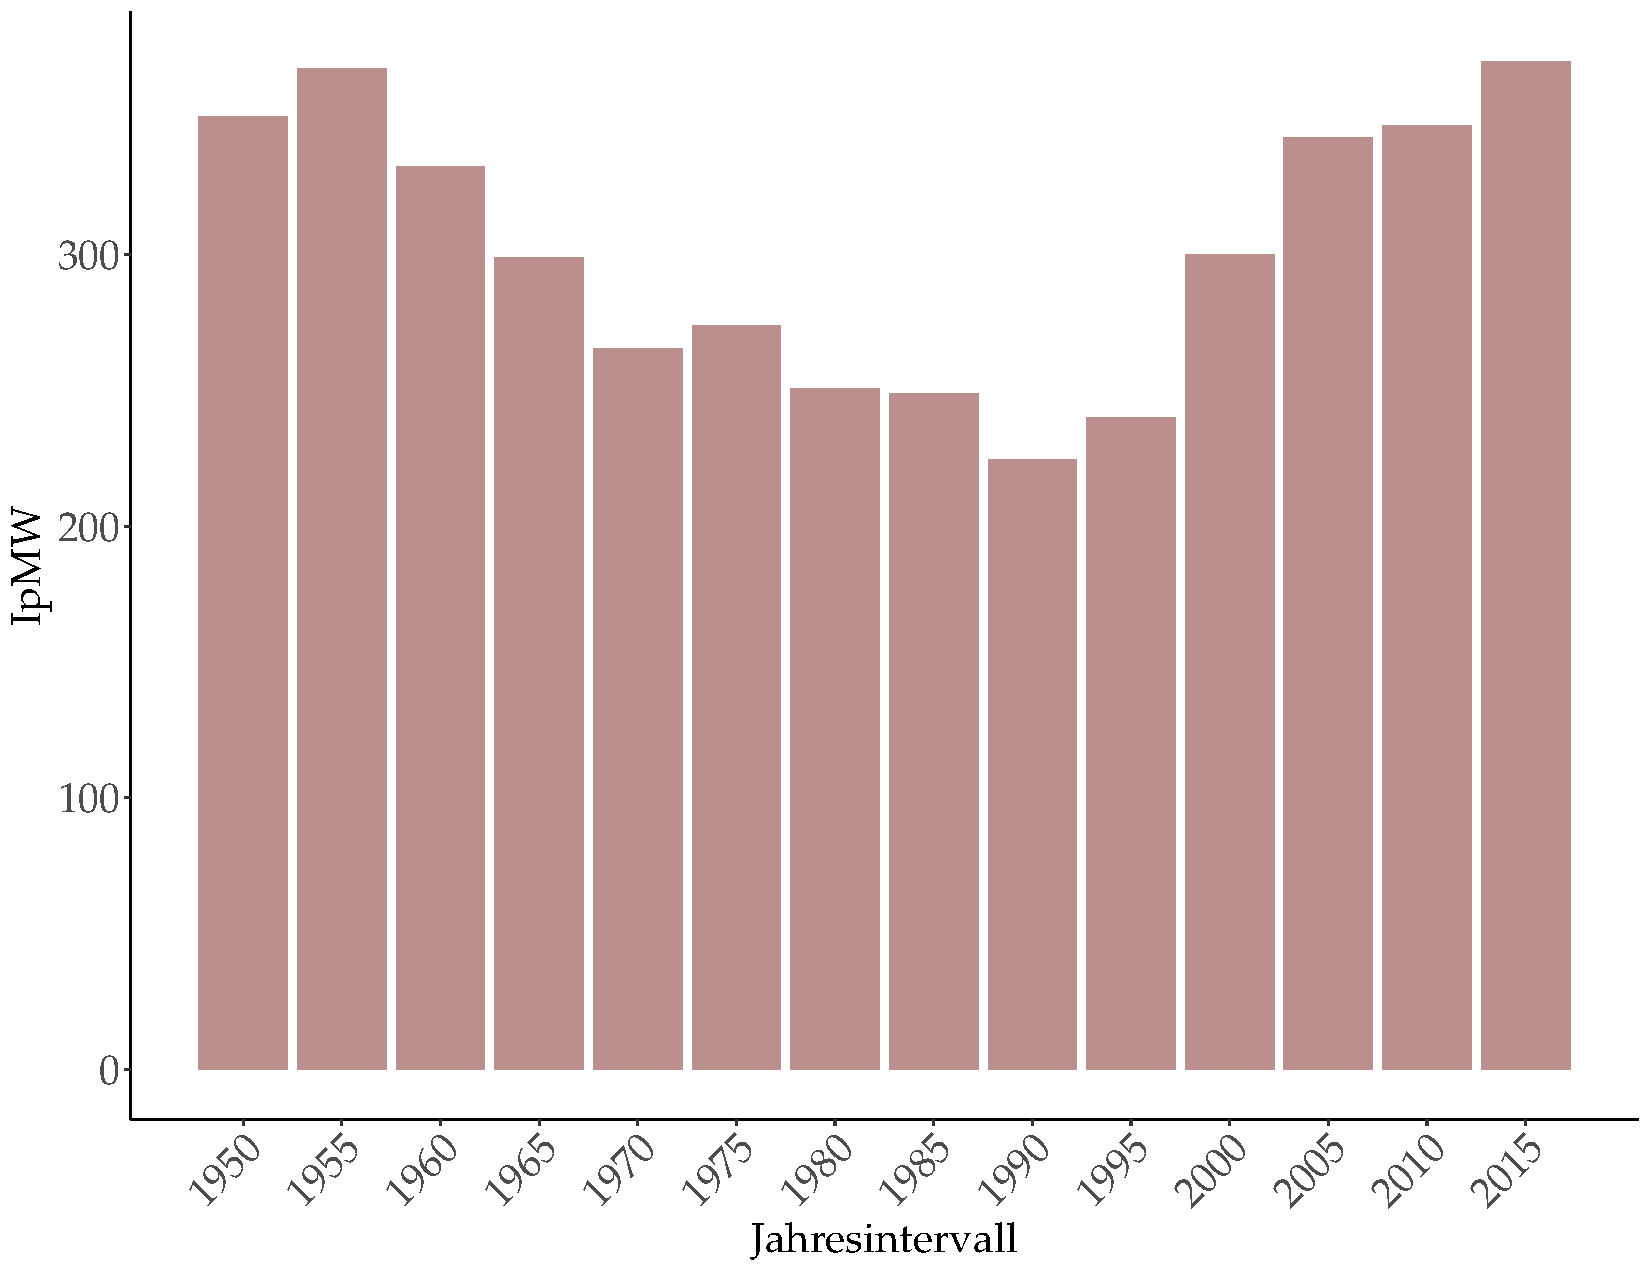
\includegraphics[width=.8\textwidth]{sehr_diachron}
  \caption[Diachrone Entwicklung des deskriptiven Intensivierers \textit{sehr} im Zeitraum von 1950 bis 2017] {Diachrone Entwicklung des deskriptiven Intensivierers \textit{sehr} im Zeitraum von Januar 1950 bis Dezember 2017 in 5-Jahresintervallen (\mbox{x-Achse} = linearer Zeitverlauf, y-Achse = relative Häufigkeit).}
  \label{Dia-sehr}
\end{figure}

Wie infolge des hohen Lexikalisierungsgrades und der darauf zurückzuführenden stark ausgeprägten Verwendungsfreiheit \citep[vgl.][420]{Breindl.2007} zu erwarten war, ist das deskriptive \textit{sehr} der mit Abstand am häufigsten verwendete Intensivierer im Zeitschriftenkorpus. Es lässt sich über den Untersuchungszeitraum mit insgesamt 20\,278,12 Treffern pro Million Textwörter nachweisen, was verdeutlicht, wie unproblematisch sein Gebrauch auch in konzeptionell schriftlichen Textsorten ist. Dieses Ergebnis stimmt mit dem Befund von \citet[266]{Ito.2003} überein, die in ihrer Korpusuntersuchung für das englische \textit{very} dieselbe Beobachtung machten. Die diachronen Häufigkeitsverteilungen für \textit{sehr} sind in \figref{Dia-sehr} dargestellt.

Dem darin abgebildeten Verlauf nach zu urteilen, fällt die Verwendung von \textit{sehr} von Mitte der Fünfzigerjahre bis zu den Neunzigerjahren hin sichtbar ab. Seinen Tiefpunkt hat der deskriptive Intensivierer im Intervall um 1990 erreicht, wohingegen sein Gebrauch seit Mitte der Neunzigerjahre wieder verstärkt zunimmt. Es zeichnet sich diachron also ein Jo-Jo-Effekt mit abnehmendem Beginn, leichter Plateau-Phase und kontinuierlich zunehmendem Ende ab. Im letzten Intervall hat sich der Gebrauch von \textit{sehr} auf einem vergleichbar hohen Niveau wie im Zeitraum von 1955 bis 1960 eingependelt. Auffällig ist, dass \textit{sehr} trotz -- oder vielmehr aufgrund -- vollständiger Delexikalisierung, Konventionalisierung und fehlender Expressivität weiterhin stark im Gebrauch ist, was zweifellos seiner textsortenadäquaten skalaren Bedeutung geschuldet ist. Dies betrifft vermutlich nicht nur das zugrunde liegende Zeitschriftenkorpus, sondern mit hoher Wahrscheinlichkeit auch die Schriftsprache im Allgemeinen. Angesichts der hohen Frequenzen und des stabilen Vorkommens lassen sich bei \textit{sehr} keinerlei konkrete Anhaltspunkte für einen allmählichen Rückgang oder gar eine Verdrängung durch andere, im Besonderen expressive Intensivierer erkennen. Auch der Versuch, den Tiefpunkt zumindest partiell mit der Frequenz der expressiven Intensivierer zu korrelieren, misslang. Demnach findet sich keine korpuslinguistische Evidenz dafür, dass \textit{sehr} in seiner rückläufigen Phase, d.\,h. im Zeitraum von 1955 bis 1990, durch andere der hier untersuchten Ausdrücke ersetzt wurde. Insofern sind die möglichen Ursachen hierfür mehr auf anderen, eventuell auch außersprachlichen Ebenen zu suchen. Diese werden in Abschnitt \ref{DisKor} näher beleuchtet. Ebenso ist nicht auszuschließen, dass die Varianz statistisch nicht signifikant und daher ohnehin zu vernachlässigen ist.

\subsection{Expressive Intensivierer}
Die untersuchten expressiven Intensivierer \textit{arg}, \textit{derb}, \textit{furchtbar}, \textit{fürchterlich}, \textit{hammer}, \textit{krass}, \textit{mega}, \textit{ober}, \textit{sau}, \textit{scheiß}, \textit{schrecklich}, \textit{super}, \textit{unheimlich}, \textit{verdammt}, \textit{voll} und \textit{wahnsinnig} (n = 16) lassen sich im Zeitschriftenkorpus mit insgesamt 1\,719,36 Treffern pro Million Textwörter nachweisen (vgl. diesbezüglich auch die Übersicht in Tabelle \ref{tab:HäuVer} im Anhang). Somit ist der deskriptive Intensivierer \textit{sehr} mit 20\,287,12 Belegen mehr als zehn Mal so häufig im Korpus repräsentiert wie alle expressiven Intensivierer zusammen. Dies bekräftigt die im Vorfeld getroffene Vermutung, nach der \textit{sehr}, ähnlich wie bei der von \citet[]{Ito.2003} durchgeführten Korpusanalyse zu englischen Intensivierern, der meistverwendete Intensivierer in den beiden Zeitschriften ist. Offen bleibt jedoch, in welchen Textsorten die gesuchten Ausdrücke aufgetreten sind. Eine solche Einschätzung war aufgrund unzureichender
textexterner Metadaten und fehlender Textsortendokumentation nicht möglich. Ungeachtet dessen scheint der diachrone Gebrauch der expressiven Intensivierer im Korpus stetig angestiegen zu sein, wobei die Zunahme in den letzten fünf Dekaden besonders stark ausgeprägt ist, wie das in \figref{Dia-rest} illustrierte Säulendiagramm demonstriert.

\begin{figure}

  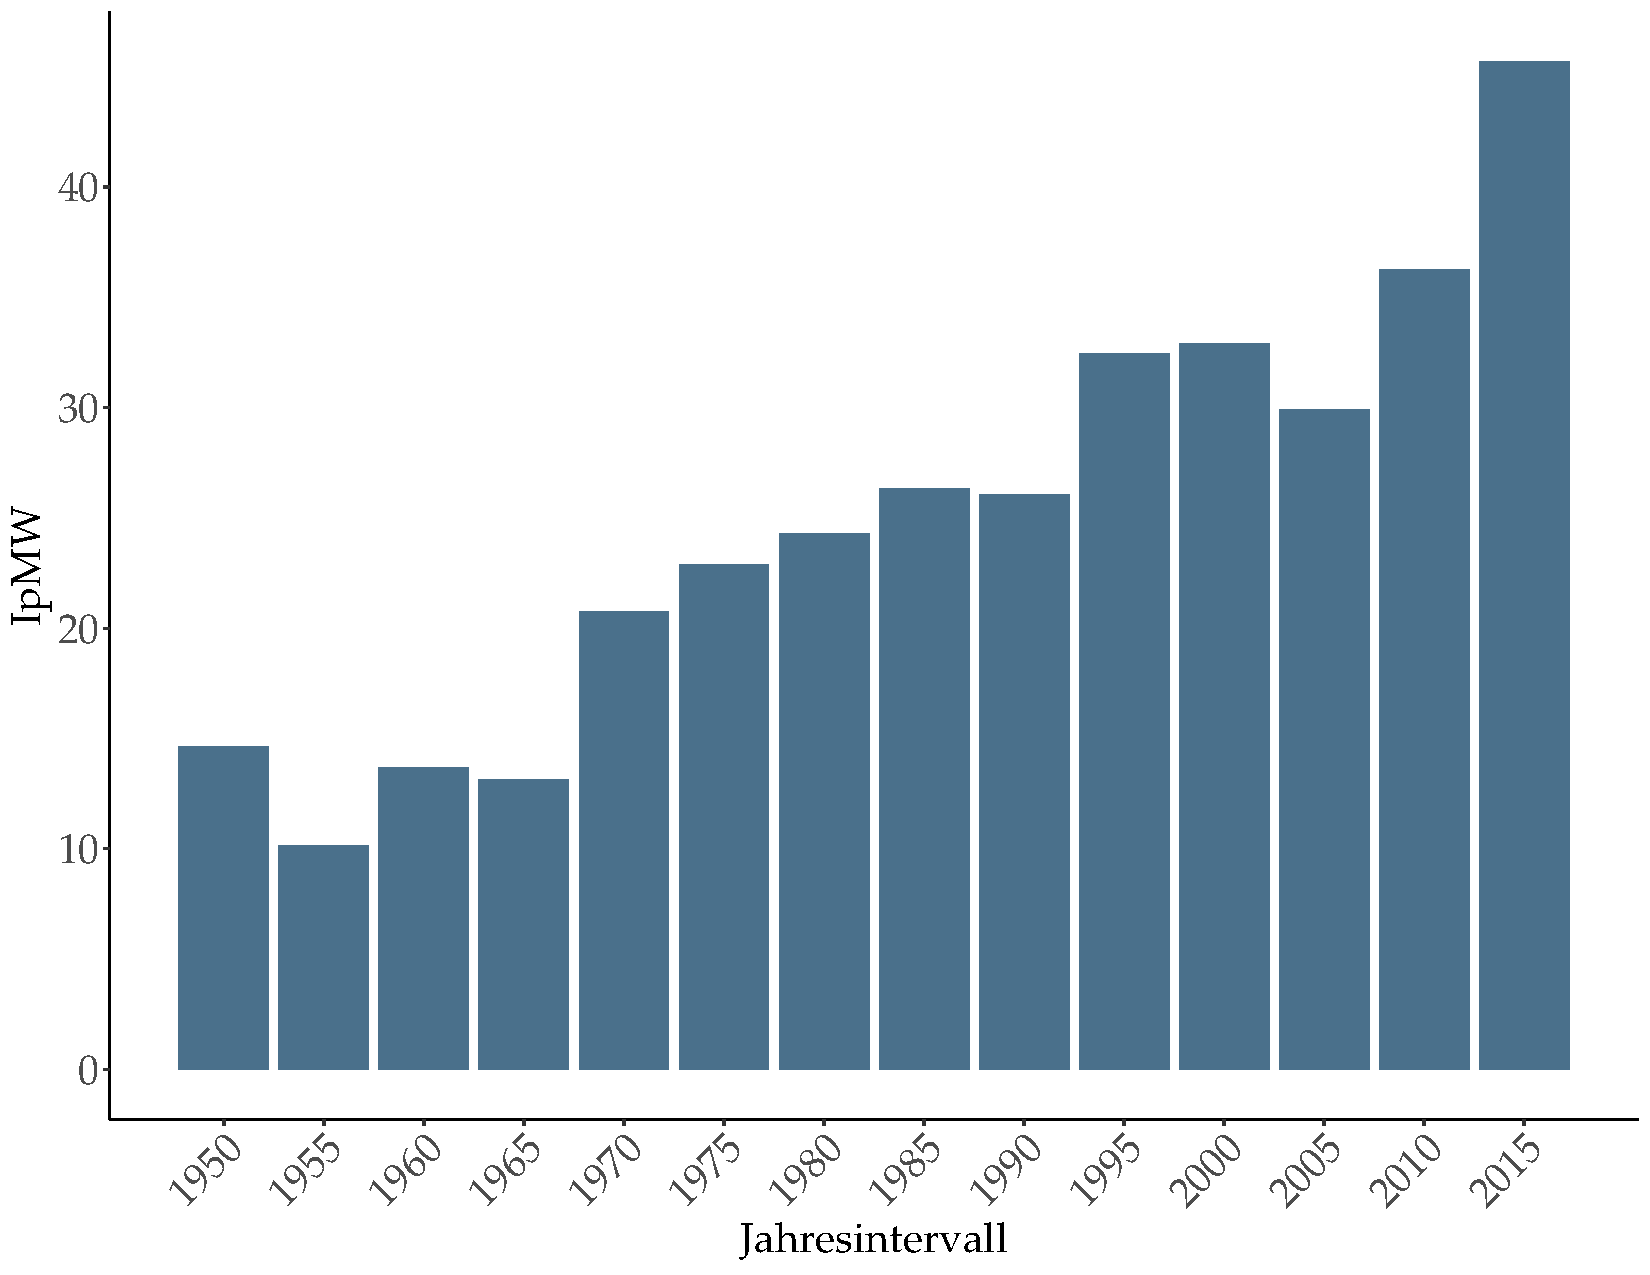
\includegraphics[width=.8\textwidth]{EI_diachron_neu.pdf}
  \caption[Diachrone Entwicklung der expressiven Intensivierer im Zeitraum von 1950 bis 2017] {Diachrone Entwicklung der expressiven Intensivierer (n = 16) im Zeitraum von Januar 1950 bis Dezember 2017 in 5-Jahresintervallen (\mbox{x-Achse} = linearer Zeitverlauf, y-Achse = relative Häufigkeit).}
  \label{Dia-rest}
\end{figure}

\noindent Der in \figref{Dia-rest} dargestellte Entwicklungsverlauf deutet auf eine positive Korrelation zwischen den Faktoren Zeit und Frequenz hin \citep[vgl.][105]{Perkuhn.2012}. So hat sich der im ersten 5-Jahresintervall gemessene IpMW-Wert von 15 bis zum letzten Intervall auf einen Wert von etwa 45 verdreifacht. Dies ist unter Berücksichtigung der eher konservativen Textsorten, aus denen sich eine Zeitschrift zusammensetzt, bemerkenswert.

Bei der Einzelbetrachtung lässt sich des Weiteren eine große Variabilität zwischen den einzelnen Ausdrücken ablesen, deren Vorkommen im Untersuchungskorpus verschieden stark ausgeprägt ist. Um dies zu veranschaulichen, sind die Entwicklungsverläufe der expressiven Intensivierer in \figref{SyDia} detailliert aufgeschlüsselt. Die Anordnung der Intensivierer erfolgt nach alphabetischer Reihenfolge. Zu beachten sind dabei die variierenden Skalen, die für die IpMW im Korpus stehen: Da die relative Frequenz der Ausdrücke stark variierte, ist die y-Achse jeweils unterschiedlich skaliert.

\begin{figure}
  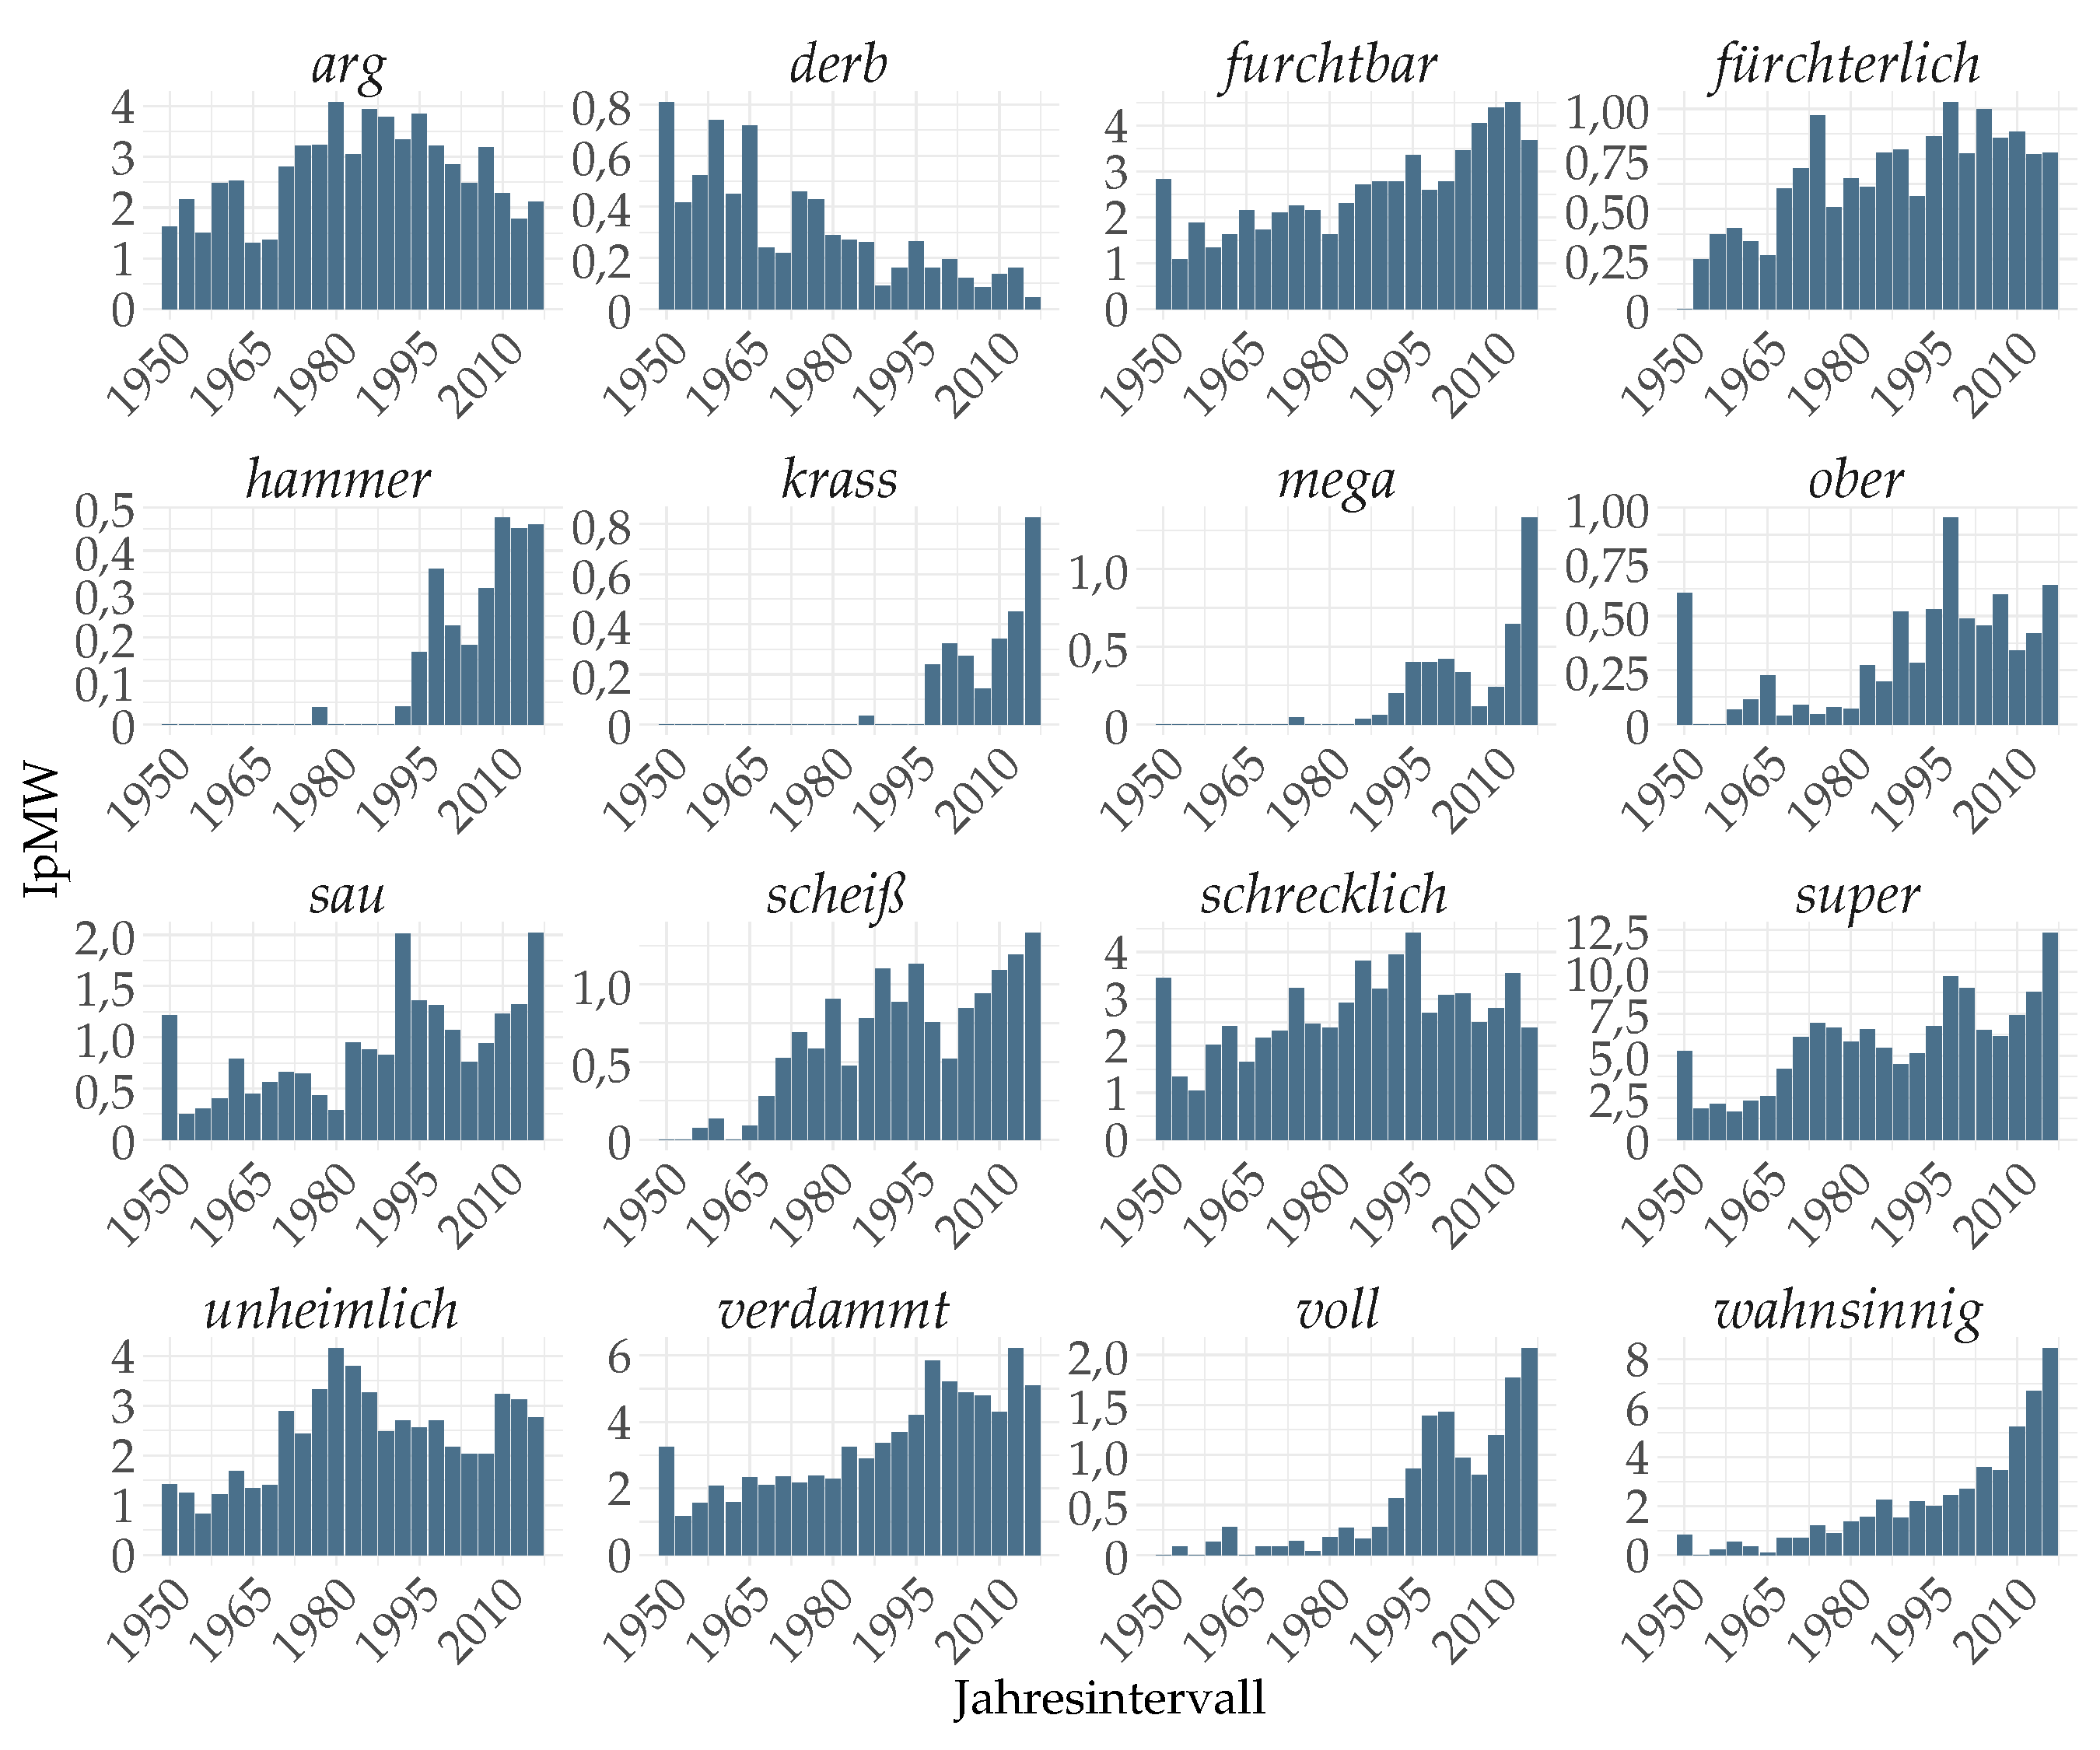
\includegraphics[width=\textwidth]{EI_facets_neu3.pdf}
  \caption [Synchrone und diachrone Entwicklung der expressiven Intensivierer im Zeitraum von 1950 bis 2017] {Synchrone und diachrone Entwicklung der expressiven Intensivierer (n = 16) im Zeitraum von Januar 1950 bis Dezember 2017 in 3-Jahresintervallen (\mbox{x-Achse} = linearer Zeitverlauf, y-Achse = relative Häufigkeiten).}
  \label{SyDia}
\end{figure}

\noindent \figref{SyDia} weist auf unterschiedliche Entwicklungsmuster der expressiven Intensivierer hin. So gibt es Ausdrücke, die über die Zeit quantitativ eher zunehmen (z.\,B. \textit{wahnsinnig}), abnehmen (\textit{derb}) oder eine schwankende, nahezu wellenartige Entwicklung anzeigen (z.\,B. \textit{arg}). Um die diachronen Verläufe der Intensivierer im Detail zu inspizieren, werden anschließend Gruppen erstellt. Die Gruppeneinteilung wird dabei im Sinne der Hypothesen -- hier insbesondere H1 -- vorgenommen. Das bedeutet, dass bei der Einteilung sowohl dem Erstvorkommen (vgl. H1-Temp) wie auch der Korpusfrequenz (vgl. H1-Freq) eine tragende Rolle zukommt. Weil der Untersuchungszeitraum von 1950 bis 2017 etwa sieben Dekaden umfasst, wird er in drei Zeitabschnitte gegliedert, in denen die Ausdrücke quantitativ eingeordnet und miteinander verglichen werden:

\newpage
\begin{enumerate}
\item Zeitraum von 1950 bis 1969
\item Zeitraum von 1970 bis 1989
\item Zeitraum von 1990 bis 2017
\end{enumerate}

\noindent Somit umfasst jeder dieser Abschnitte 20 Jahre, wobei letzterem darüber hinaus auch die restlichen acht Jahre zugeschrieben werden. Wie \citet[97]{Perkuhn.2012} erklären, gibt es keine allgemeingültige Systematik hinsichtlich der Segmentierung von Korpora, was in Anbetracht der Variation von Korpusuntersuchungen wenig überraschend ist. Dementsprechend müssen korpuslinguistisch Forschende stets individuelle Segmentierungen unter Berücksichtigung ihrer Datengrundlage und Zielsetzung vornehmen. Um der verfolgten Fragestellung Rechnung zu tragen, ist meiner Ansicht nach eine Einteilung des Untersuchungskorpus in 20-Jahresschritte aus verschiedenen Gründen eine zielführende Vorgehensweise: Einerseits braucht es einige Zeit, bis sich typischerweise mündlichkeitsnahe Phänomene wie Intensitätspartikeln in der als eher konservativ geltenden Zeitungssprache etablieren. Aus diesem Grund sollte die Zeitspanne nicht zu knapp bemessen sein, wenn man valide Aussagen über die Entwicklung der Ausdrücke treffen möchte. Andererseits sollte die Zeitspanne jedoch auch nicht zu umfassend gewählt sein, da man sonst Gefahr läuft, potenziell bedeutsame Entwicklungsschritte zu übersehen oder zu verallgemeinern. Schaut man sich die Entwicklungsverläufe der expressiven Intensivierer in den Abbildungen \ref{Dia-rest} und \ref{SyDia} an, so scheinen Intervalle von 20 Jahren eine gute Grundlage zu sein, anhand derer der Fortgang der Ausdrücke in Bezug auf die Hypothesen abgeglichen werden kann. So bildet das Ende dieses Zeitraums oftmals die Trennlinie für offensichtliche Veränderungen, wie bspw. an dem um 1970 herum ausgeprägten Tiefpunkt von \textit{arg} und \textit{derb} zu erkennen ist.

Neben der zeitlichen Dimension, die Rückschlüsse auf das Erstvorkommen der Ausdrücke ermöglicht und überdies erste Hinweise auf das Zutreffen der Hypothese H2 liefert, wird die Häufigkeit der Intensivierer pro Segment begutachtet. In diesem Kontext stellt sich die Frage, welche expressiven Intensivierer in den Zeitabschnitten hoch- und welche niedrigfrequent sind. Aus Gründen der Vollständigkeit wird \textit{sehr} als Vertreter der deskriptiven Intensiviererklasse ebenso einer solchen Begutachtung unterzogen, wenn auch die Expressivität hier nicht als Erklärung für die zu beobachtenden Verläufe in Erwägung gezogen wird. Aufgrund dessen, dass es sich um einen einzelnen Ausdruck handelt, wird für \textit{sehr} zunächst jede Dekade separat aufgeführt, woraus sich schließlich die kumulierten Werte für die oben erläuterten Zeitabschnitte (d.\,h. 1950 bis 1969, 1970 bis 1989 und 1990 bis 2017) ergeben.

Ehe die Ergebnisse der Auswertung vorgestellt werden, sei darauf hingewiesen, dass die Grenzen keineswegs als trennscharf zu beurteilen sind. Dennoch lassen die Tendenzen bedeutsame Mutmaßungen über den Gebrauch der Ausdrücke (stellvertretend für konventionell schriftliche Kontexte) zu.

\subsection[Segmentale Entwicklung des deskriptiven Intensivierers]{Segmentale Entwicklung des deskriptiven Intensivierers}
Wie in Abschnitt \ref{DeSehr} geschildert, lässt sich die diachrone Entwicklung von \textit{sehr} als eine Art Welle mit abnehmendem Beginn, verhältnismäßig niedrigerer Plateau-Phase und ansteigendem Ende beschreiben.

Aus diesem Grund ist es interessant, sich die kumulierte Häufigkeitsverteilung des deskriptiven Intensivierers über den Untersuchungszeitraum von 1950 bis 2017 genauer anzuschauen. Die Frequenzen von \textit{sehr} je Dekade sind in chronologischer Reihenfolge in Tabelle \ref{Fre0} zusammengetragen.

%%%%%%%%%%%

\begin{table}
\fittable{
\begin{tabular}{l@{~}rrc@{}r@{~}}
\lsptoprule
{Jahrzehnt} & Absolute  Frequenz  & Relative Frequenz  & & Kumulierte Frequenz \\
\midrule
1950--1959 & 12\,638 & 3\,522,92 & \rdelim\}{2}{.4cm} & {\multirow{2}{*} {6\,714,94}}\\
1960--1969 & 20\,949 & 3\,192,02 &  & \\
\tablevspace
1970--1979 & 21\,192 & 2\,692,41 & \rdelim\}{2}{.4cm} & {\multirow{2}{*} {5\,190,35}}\\
1980--1989 & 24\,662 & 2\,497,94 &  & \\
\tablevspace
1990--1999 & 21\,770 & 2\,605,88 &  \rdelim\}{3}{.4cm} & {\multirow{3}{*} {8\,372,83}} \\
2000--2009 & 34\,632 & 2\,916,41 &  & \\
2010--2017 & 29\,318 & 2\,850,54 &  & \\
\midrule
In Summe & 165\,161 & 2\,0278,12 &  &\\
\lspbottomrule
\end{tabular}
}
\caption[Kumulierte Häufigkeitsverteilung des deskriptiven Intensivierers im Zeitraum von 1950 bis 2017]{Kumulierte Häufigkeitsverteilung des deskriptiven Intensivierers \textit{sehr} im Zeitraum von 1950 bis 2017 (in chronologischer Reihenfolge).}
\label{Fre0}
\end{table}

\noindent Wie das in \figref{Dia-sehr} dargestellte Histogramm vermuten lässt, geben auch die Korpusfrequenzen von \textit{sehr} eine zunächst rückläufige Entwicklung an. So gehen die in den ersten beiden Dekaden ermittelten Frequenzen von über 3\,000 Treffern sukzessive derart zurück, dass der Intensivierer im Zeitraum von 1980 bis 1989 mehr als 1\,000 Korpusbelege weniger als in der ersten Dekade aufweist. Nach dem Tiefpunkt nimmt \textit{sehr} in seiner Frequenz schließlich wieder zu, sodass das Intervall von 2000 bis 2009 vergleichbar mit dem zweiten Intervall von 1960 bis 1969 ist. Da der letzte Zeitabschnitt aufgrund des beschränkten Untersuchungszeitraums lediglich bis Dezember 2017 reicht und somit noch 24 Monate bis zur Vollendung der siebten Dekade ausstehen, lassen sich die fehlenden Werte an dieser Stelle nur extrapolieren. Ausgehend von der Vermutung, dass die Verwendung von \textit{sehr} in den Jahren 2018 und 2019 in etwa gleich stark ausgeprägt ist, ist zu erwarten, dass das kumulierte Vorkommen in diesem Jahrzehnt dem aus dem ersten weitgehend in Nichts nachsteht. Dies lässt darauf schließen, dass der deskriptive Intensivierer seine quantitative Einbuße überstanden und sich der Gebrauch im Korpus nach temporärem Rückgang bis zur vierten Dekade schließlich zum Positiven gewendet hat. Gegenwärtig liegt der Gebrauch von \textit{sehr} im Zeitschriftenkorpus in etwa auf einem vergleichbar hohen Frequenzniveau wie zu Beginn des Untersuchungszeitraums.

\subsection{Segmentale Entwicklung der expressiven Intensivierer}
Anders als bei \textit{sehr} erfolgt die Begutachtung der expressiven Intensivierer direkt separiert nach den oben umschriebenen Zeitspannen. Dies gewährt zum einen einen besseren Überblick über die Häufigkeitsverteilungen. Zum anderen ermöglicht es auch eine zielgerichtetere Gegenüberstellung der Ausdrücke. Auf Basis der bezüglich H1 relevanten Faktoren Erstvorkommen (vgl. H1-Temp) und Frequenz (vgl. H1-Freq) werden die expressiven Intensivierer sukzessive hierarchisch klassifiziert. Im Zuge dessen wird im ersten Analyseschritt für jeden Zeitabschnitt überprüft, welche der Ausdrücke im Korpus alt und welche neu sind. Exemplarisch wird am zweiten Intervall daher der Frage nachgegangen, welche Ausdrücke es schon vor 1969 gab und welche erst anschließend erstmals in intensivierender Funktion in Erscheinung treten. Im zweiten Analyseschritt wird die Frequenz beleuchtet: So lassen sich in jedem Intervall zwei Frequenzgruppen ausmachen, deren Zusammensetzung eingehend in Augenschein genommen wird.

Unterstützt wird diese erste Einteilung durch eine mit R vorgenommene hierarchische agglomerative Clusteranalyse, die mit dem Ziel durchgeführt wurde, durch die daraus abgeleiteten Dendrogramme Ähnlichkeiten zwischen den Intensivierern aufzudecken. Dabei handelt es sich um ein exploratives Bottom-up-Verfahren, mit dem es auf Grundlage der Ergebnisse möglich ist, Hypothesen für weitere Untersuchungen aufzustellen \citep[vgl.][294]{Gries.2008}. Auf diese Weise lässt sich mithilfe einer grafischen Visualisierung einschätzen, ob die erste, intuitiv unternommene Gruppeneinteilung treffend ist oder revidiert bzw. \mbox{justiert} werden muss. Bei einer solchen Analyse wird eine Anzahl von Objekten (hier: Intensivierer) gemäß bestimmter Merkmale (hier: Frequenzen) in verschiedene Cluster eingeteilt. Die Eingruppierung der Ausdrücke wird durch das relative Vorkommen der Ausdrücke im Korpus, d.\,h. die IpMW, generiert. Der Ausgangspunkt liegt bei 16 Einzelgruppen, alle expressiven Intensivierer also, die mittels einer Distanzmatrix zu homogenen Gruppen zusammengefasst werden. Die Eigenschaften der Mitglieder eines Clusters ähneln sich, während sie sich von den Mitgliedern anderer Gruppen hingegen unterscheiden. Demzufolge sind die Intensivierer innerhalb eines Clusters hinsichtlich der Korpusfrequenz homogen und heterogen zu den Intensivierern der anderen Cluster. Dabei gilt: Je niedriger die Distanz zwischen den einzelnen Gruppen ist, desto ähnlicher sind sich die Ausdrücke. Oder andersherum ausgedrückt: Je größer die Distanz zwischen den einzelnen Gruppen ist, desto unähnlicher sind sie sich im Hinblick auf ihre Korpusfrequenz (vgl. \mbox{\citealt[296]{Gries.2008}}; \mbox{\citealt[440]{Backhaus.2018}}; \mbox{\citealt[437ff.]{Sauer.2019}}).

Die für die jeweiligen Zeitabschnitte abgeleiteten Dendrogramme befinden sich unter den Ausführungen zu den Frequenzen eines jeden Intervalls. In diesen sind die expressiven Intensivierer in Form einer grafischen Baumstruktur auf Grundlage der Euklidischen Distanz\footnote{Die Euklidische Distanz ist das Maß, das die Ähnlichkeit bzw. Unähnlichkeit der Intensivierer auf Grundlage ihrer Entfernung voneinander numerisch ausdrückt. Nach \citet[450]{Backhaus.2018} werden dabei \glqq{}für jedes Objektpaar die Differenzwerte jeder Eigenschaft quadriert und anschließend addiert\grqq{}, woraufhin aus der Summe die Quadratwurzel gezogen wird.} in verschiedene, homogene Cluster eingruppiert. Die x-Achse symbolisiert die Distanz, auf deren Basis sich Rückschlüsse in Bezug auf die Gemeinsamkeiten bzw. Unterschiede der Ausdrücken ziehen lassen, die y-Achse steht für den Grad der Ähnlichkeit der Ausdrücke und repräsentiert das Fusionskriterium. Die Verschmelzung der Intensivierer erfolgte durch das Ward-Verfahren (\citealt[]{Ward.1963}),\footnote{Anders als andere Methoden gruppiert das Ward-Verfahren als varianzanalytische Amalgamierungsregel Objekte, die keinen großen Einfluss auf ein vorgegebenes Heterogenitätsmaß bzw. Varianzkriterium ausüben. Dadurch wird die Streuung innerhalb einer Gruppe so wenig wie möglich erhöht und die Fehlerquadratsumme entsprechend niedrig gehalten {(vgl. \citealt[305]{Gries.2008}; \citealt[465f.]{Backhaus.2018}}).} das nach möglichst homogenen Clustern strebt \citep[vgl.][305]{Gries.2008}. Nachdem das genaue Vorgehen transparent gemacht wurde, folgt im nächsten Part die Betrachtung des ersten Zeitabschnitts, d.\,h. des Zeitraums von 1950 bis 1969.

\subsubsection{Zeitabschnitt von 1950 bis 1969}
Im ersten Zeitabschnitt finden sich im Korpus 13 expressive Intensivierer, die mit insgesamt 277,76 Treffern pro Million Textwörter auftreten. Begonnen wird jeweils mit denjenigen Ausdrücken, die eine niedrige Frequenz aufweisen. Dies betrifft im ersten Intervall \textit{scheiß}, \textit{voll}, \textit{ober}, \textit{fürchterlich}, \textit{wahnsinnig}, \textit{sau} und \textit{derb} (n = 7). Die Gruppe der niedrigfrequenten Intensivierer bewegt sich quantitativ in einem Rahmen von 0 bis ca. 12 Belegen (${\scriptstyle \sum{}}$ = 41,53)\footnote{Das Symbol Sigma (${\scriptstyle \sum{}}$) meint hier und im Folgenden die Summe der relativen Frequenzen.}. Die zweite Gruppe beinhaltet dagegen diejenigen Ausdrücke, deren relative Frequenz im Korpus bei mehr als 25 Treffern liegt (${\scriptstyle \sum{}}$ = 236,23): \textit{unheimlich}, \textit{furchtbar}, \textit{arg}, \textit{verdammt}, \textit{schrecklich} und \textit{super} (n = 6). Zur Illustration sind die beiden Gruppen mitsamt der jeweiligen kumulierten Frequenz der Mitglieder in Tabelle \ref{Fre1} abgebildet. Die Sortierung der Intensivierer je Gruppe erfolgt in zunehmender Frequenz.

%%%%%%%%%%%%%%%%%

\begin{table}
\begin{tabularx}{\textwidth}{l@{}>{\raggedleft}p{2cm}@{}>{\raggedleft}p{2cm}@{}>{\raggedleft}p{2.5cm}@{~}r@{}Y}
\lsptoprule
{Intensivierer} & {Absolute} Frequenz & {Relative} Frequenz & {Prozentualer} Anteil & & {Klassifikation} \\
\midrule
\textit{scheiß} & {7} & {1,18} & {0,42\,\%} & \rdelim\}{7}{.3cm} & \\
\textit{voll} & {9} &{1,68} & {0,60\,\%} & &\\
\textit{ober} & {11} &{3,01} & {1,08\,\%} & & \multirow{3}{*}{\parbox{2.5cm}{{niedrigfrequent \\ (14,95\,\%)}}} \\
\textit{fürchterlich} & {37} &{6,27} & {2,26\,\%} & &  \\
\textit{wahnsinnig} & {29} & {6,90} & {2,48\,\%} & & \\
\textit{sau} & {49} &{10,78} & {3,88\,\%} & & \\
\textit{derb} & {55} &{11,71} & {4,22\,\%} & &\\
\midrule
\textit{unheimlich} & {131} &{25,69} & {9,25\,\%} & \rdelim\}{6}{.3cm} & \\
\textit{furchtbar} & {173} & {35,73} & {12,86\,\%} & &  \multirow{4}{*}{\parbox{2.5cm}{{hochfrequent \\ (85,05\,\%)}}}\\
\textit{arg} & {191} &{38,21} & {13,76\,\%} & & \\
\textit{verdammt} & {195} &{39,94} & {14,38\,\%} & & \\
\textit{schrecklich} & {194} &{40,65} & {14,63\,\%} & &\\
\textit{super} & {263} &{56,01} & {20,16\,\%} & &\\
\midrule
In Summe & {1\,344} & {277,76} & {100\,\%} & &\\
\lspbottomrule
\end{tabularx}
\caption[Kumulierte Häufigkeitsverteilungen der expressiven Intensivierer im Zeitraum von 1950 bis 1969]{Kumulierte Häufigkeitsverteilungen der expressiven Intensivierer im Zeitraum von 1950 bis 1969 (angeordnet nach zunehmender Frequenz).}
\label{Fre1}
\end{table}

\noindent Wie sich aus Tabelle \ref{Fre1} ablesen lässt, verfügt \textit{unheimlich} über die niedrigste Trefferquote von Gruppe 2. Dennoch ist dieser Wert mehr als doppelt so hoch wie die Trefferzahl von \textit{derb}, das in Gruppe 1 mit 11,71 Treffern pro Million Textwörter die höchste Frequenz aufweist. Infolge dieser recht ausgeprägten Differenz scheint eine Grenze an dieser Stelle, d.\,h. zwischen \textit{derb} und \textit{unheimlich}, gerechtfertigt. Interessanterweise liegen die Intensivierer \textit{furchtbar}, \textit{arg}, \textit{verdammt} und \textit{schrecklich}, die qua Semantik einen negativen Zustand denotieren, zahlenmäßig eng beieinander. Demgegenüber ist \textit{super} in diesem Intervall mit 56 Korpusbelegen sogar doppelt so häufig in den beiden Zeitschriften zu finden wie \textit{unheimlich}. Auffällig ist weiterhin auch, dass die Intensivierer \textit{hammer}, \textit{mega} und \textit{krass} im ersten Zeitabschnitt überhaupt nicht vorkommen. Bei ihnen handelt es sich also um Ausdrücke, die sich erst innerhalb des Untersuchungszeitraums als Intensivierer im Korpus neu herausgebildet haben.

In \figref{Dendro1} ist das für den Zeitraum von 1950 bis 1969 einschlägige Dendrogramm dargestellt. Anhand diesem lässt sich überprüfen, ob die in der obigen Tabelle skizzierte Gruppeneinteilung zutreffend ist.

\begin{figure}

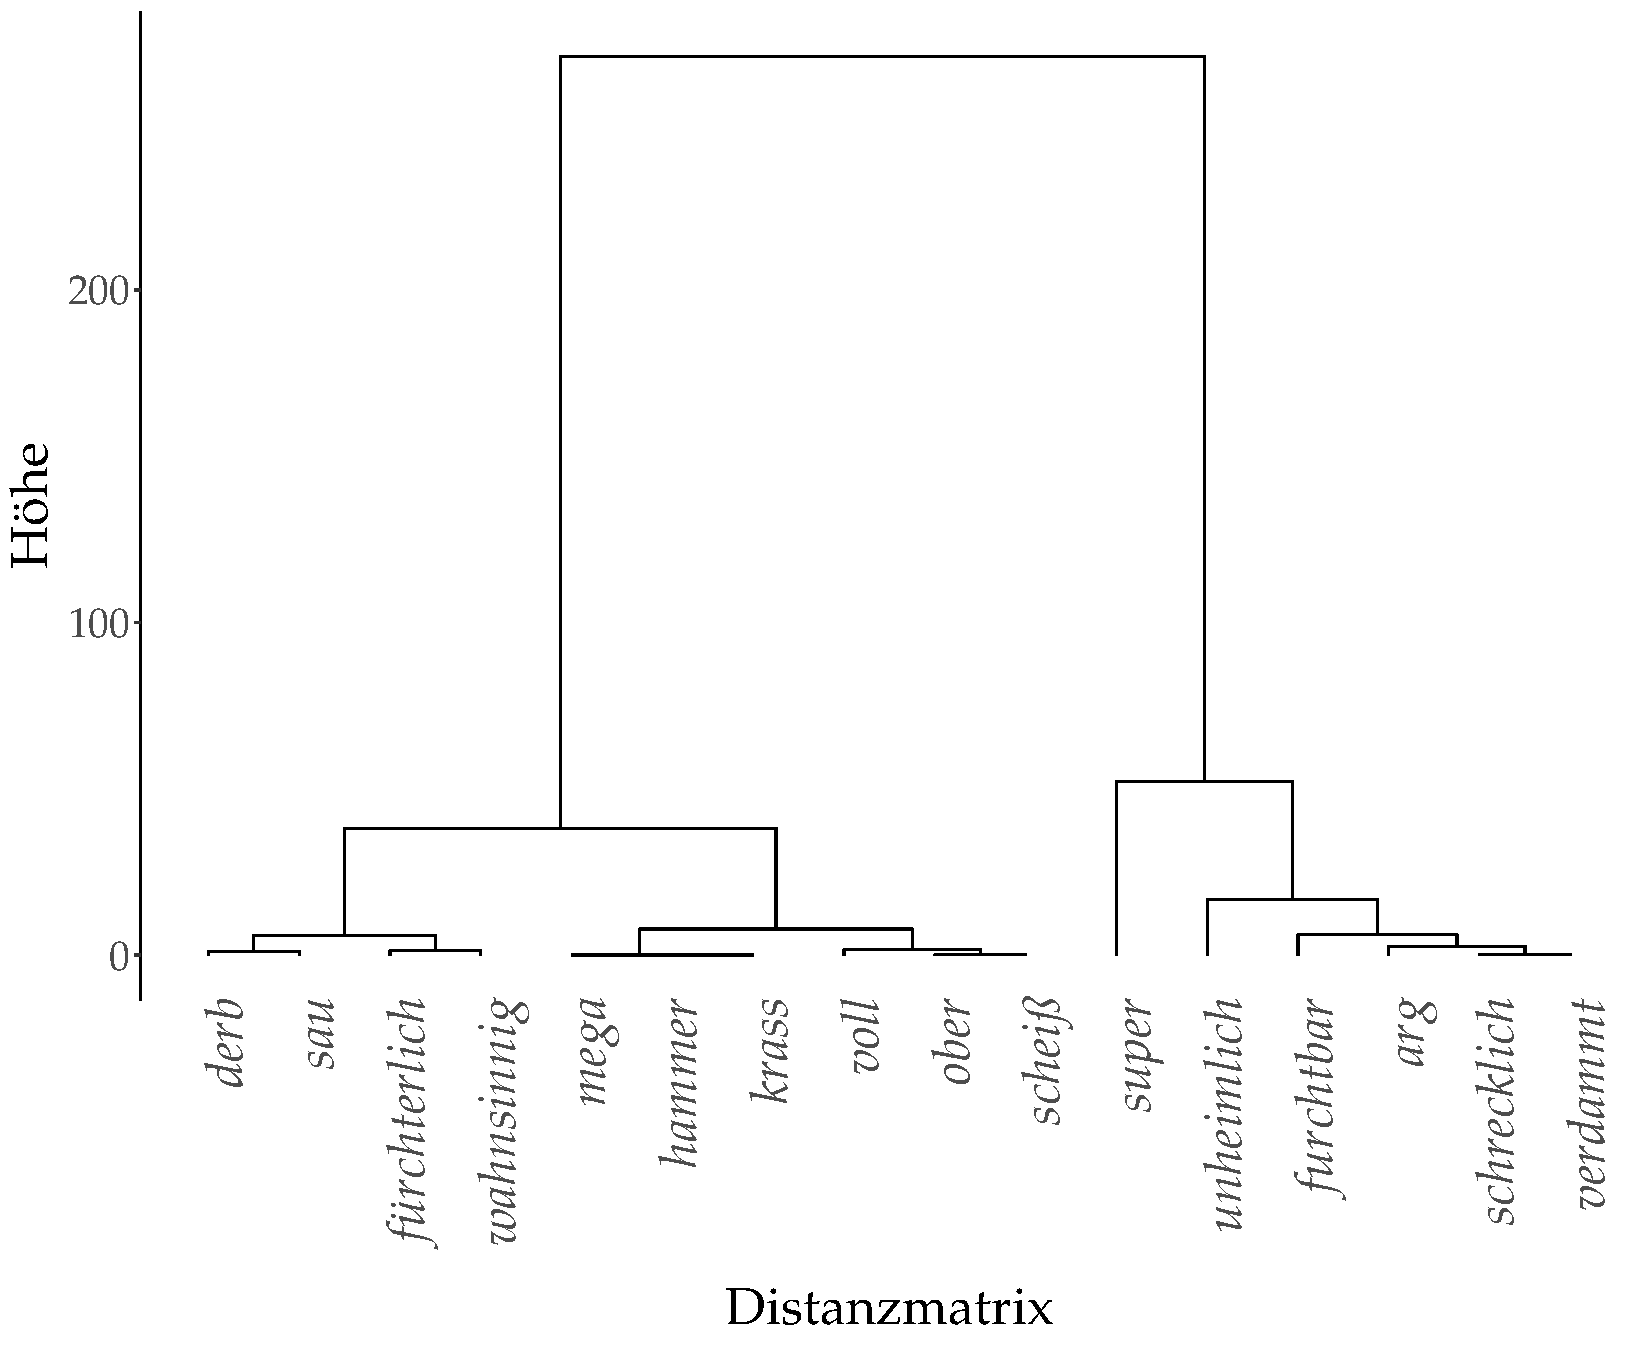
\includegraphics[width=1\textwidth]{1950-1969}
\caption[Cluster-Dendrogramm der expressiven Intensivierer für den Zeitraum von 1950 bis 1969]{Cluster-Dendrogramm der expressiven Intensivierer für den Zeitraum von 1950 bis 1969 (Maß: Euklidische Distanz; Amalgamierungsmethode: Ward-Verfahren (\citealt[]{Ward.1963})).}
\label{Dendro1}
\end{figure}

\noindent Das Dendrogramm aus \figref{Dendro1} zeigt zwei große Cluster mit mehreren Subclustern. Das linke Cluster beinhaltet dabei sowohl diejenigen Intensivierer, die sich in diesem Zeitabschnitt im Korpus überhaupt nicht nachweisen lassen (d.\,h. \textit{mega}, \textit{hammer} und \textit{krass}), als auch solche, die mit einer niedrigen Frequenz auftreten: \textit{derb}, \textit{sau}, \textit{fürchterlich}, \textit{wahnsinnig}, \textit{voll}, \textit{ober} und \textit{scheiß}. Intensivierer, die über homogene Merkmale verfügen, also  ähnlich frequent sind, werden zudem in weiteren Subclustern zusammengefasst, was u.\,a. am Beispiel von \textit{derb} und \textit{sau} zu sehen ist. Auf der anderen Seite finden sich im rechten Cluster diejenigen Intensivierer, die im Korpus deutlich frequenter sind, nämlich \textit{super}, \textit{unheimlich}, \textit{furchtbar}, \textit{arg}, \textit{schrecklich} und \textit{verdammt}. Wie bereits im Hinblick auf Tabelle \ref{Fre1} angesprochen, beinhaltet diese Gruppe mit Ausnahme von \textit{super} ausschließlich Ausdrücke mit klar negativer Quellsemantik, die die durch das Adjektiv ausgedrückte Eigenschaft in Form von Furcht, Angst und Schrecken verstärken (vgl. \citealt[165ff.]{Biedermann.1969}; \citealt[]{Hentschel.1998b}). Aufgrund vergleichbarer Frequenzen liegen diese Ausdrücke auch im Dendrogramm nahe beieinander. Wie das Fusionskriterium nahelegt, unterscheidet sich der Intensivierer \textit{super} stark von den restlichen Gruppenmitgliedern, was dessen ungleich höherer Korpusfrequenz geschuldet ist. Das Dendrogramm des ersten Zeitabschnitts scheint also die zuvor angenommene Gruppeneinteilung aus Tabelle \ref{Fre1} vollständig zu stützen, sodass keine Nachjustierungen erforderlich sind.

\subsubsection{Zeitabschnitt von 1970 bis 1989}
Im zweiten Intervall sind alle 16 expressiven Intensivierer mit einer kumulierten Gesamtfrequenz von 485,56 Treffern im Zeitschriftenkorpus vertreten. Davon verfügen die Ausdrücke \textit{krass}, \textit{hammer}, \textit{mega}, \textit{ober}, \textit{voll}, \textit{derb}, \textit{sau}, \textit{scheiß} und \textit{fürchterlich} (n = 9) über ein niedriges Vorkommen. Diese weisen im Zeitraum von 1970 bis 1989 maximal 14 Korpusbelege auf (${\scriptstyle \sum{}}$ = 53,41). Auf der anderen Seite finden sich hingegen die Intensivierer \textit{wahnsinnig}, \textit{furchtbar}, \textit{verdammt}, \textit{schrecklich}, \textit{unheimlich}, \textit{arg} und \textit{super} (n = 7), die mit mindestens 26 Treffern merklich frequenter sind (${\scriptstyle \sum{}}$ = 432,15). Wie zuvor sind die genauen Korpusfrequenzen im Sinne der Übersichtlichkeit tabellarisch dargestellt (vgl. Tabelle \ref{Fre2}). Auch hier erfolgt die Anordnung jeweils nach zunehmender Frequenz.

\begin{table}
\begin{tabularx}{\textwidth}{l@{}>{\raggedleft}p{2cm}@{}>{\raggedleft}p{2cm}@{}>{\raggedleft}p{2.5cm}@{~}r@{}Y}
\lsptoprule
{Intensivierer} & {Absolute}  Frequenz& {Relative} Frequenz& {Prozentualer} Anteil& & {Klassifikation} \\
\midrule
\textit{krass} & {1} & {0,10} & 	{0,02\,\%}		& \rdelim\}{9}{.3cm} & \\
\textit{hammer} & {1} & {0,12} &	{0,02\,\%}		& 			&\\
\textit{mega} & {2} &{0,24}& 		{0,05\,\%}	& &\\
\textit{ober} & {27} & {2,83} &		{0,58\,\%}	& &  \multirow{3}{*}{\parbox{2.5cm}{{niedrigfrequent \\ (11,02\,\%)}}} \\
\textit{voll} & {29} & {3,15} &		{0,65\,\%}	& & \\
\textit{derb} & {52} &{6,00} 	&	{1,24\,\%}	& &  \\
\textit{sau} & {121} & {13,41} &		{2,77\,\%}	& &\\
\textit{scheiß} & {123} & {13,71} &	{2,83\,\%}	& &\\
\textit{fürchterlich} & {122} & {13,85} &	{2,86\,\%} & &\\
\midrule
\textit{wahnsinnig} & {239} & {26,15} & {5,19\,\%} & \rdelim\}{7}{.3cm} & \\
\textit{furchtbar} & {403} & {44,99} & {9,28\,\%} & &\\
\textit{verdammt} & {460} & {51,26} &  {10,58\,\%} & &  \multirow{3}{*}{\parbox{2.5cm}{{hochfrequent \\ (88,98\,\%)}}} \\
\textit{schrecklich} & {508} & {56,55}& {11,67\,\%} & & \\
\textit{unheimlich} & {579} & {64,23} & {13,26\,\%} & & \\
\textit{arg} & {602} & {66,85}& {13,80\,\%} & &\\
\textit{super}  & {1\,075} &  {122,12}& {25,20\,\%} & &\\

\midrule
In Summe & {4\,344} & {485,56} & {100\,\%} &  &\\
\lspbottomrule
\end{tabularx}
\caption[Kumulierte Häufigkeitsverteilungen der expressiven Intensivierer im Zeitraum von 1970 bis 1989]{Kumulierte Häufigkeitsverteilungen der expressiven Intensivierer im Zeitraum von 1970 bis 1989 (angeordnet nach zunehmender Frequenz).}
\label{Fre2}
\end{table}

%%%%%%%%%%%%%%%%%%

Da \textit{wahnsinnig} im Korpus beinahe doppelt so frequent ist wie \textit{fürchterlich}, erscheint mir eine Grenze an dieser Stelle sinnvoll. Die im Korpus neu entwickelten Intensivierer \textit{krass}, \textit{mega} und \textit{hammer} weisen in diesem Zeitabschnitt eine nur geringe Frequenz auf. Daneben hat sich innerhalb von Gruppe 1 die häufigkeitsbedingte Anordnung geändert, sodass \textit{fürchterlich} hier nun am häufigsten ist. Der im vorigen Zeitabschnitt niedrigfrequente Intensivierer \textit{wahnsinnig} ist in diesem Intervall in die Gruppe der hochfrequenten Intensivierer übergetreten, sodass diese auf insgesamt sieben Mitglieder angewachsen ist. Darin lässt sich \textit{super} als einziger Intensivierer mit mehr als 100 Belegen nachweisen, sodass er seine Spitzenposition stark ausgebaut hat. Bei den restlichen Ausdrücken dieser Gruppe handelt es sich mit \textit{wahnsinnig}, \textit{furchtbar}, \textit{verdammt}, \textit{schrecklich}, \textit{unheimlich} und \textit{arg} noch immer ausschließlich um solche, die sich durch eine transparente negative Semantik auszeichnen. Auch diese Intensivierer sind im Vergleich zum vorangegangenen Intervall in einer anderen Reihenfolge angeordnet.


\begin{figure}

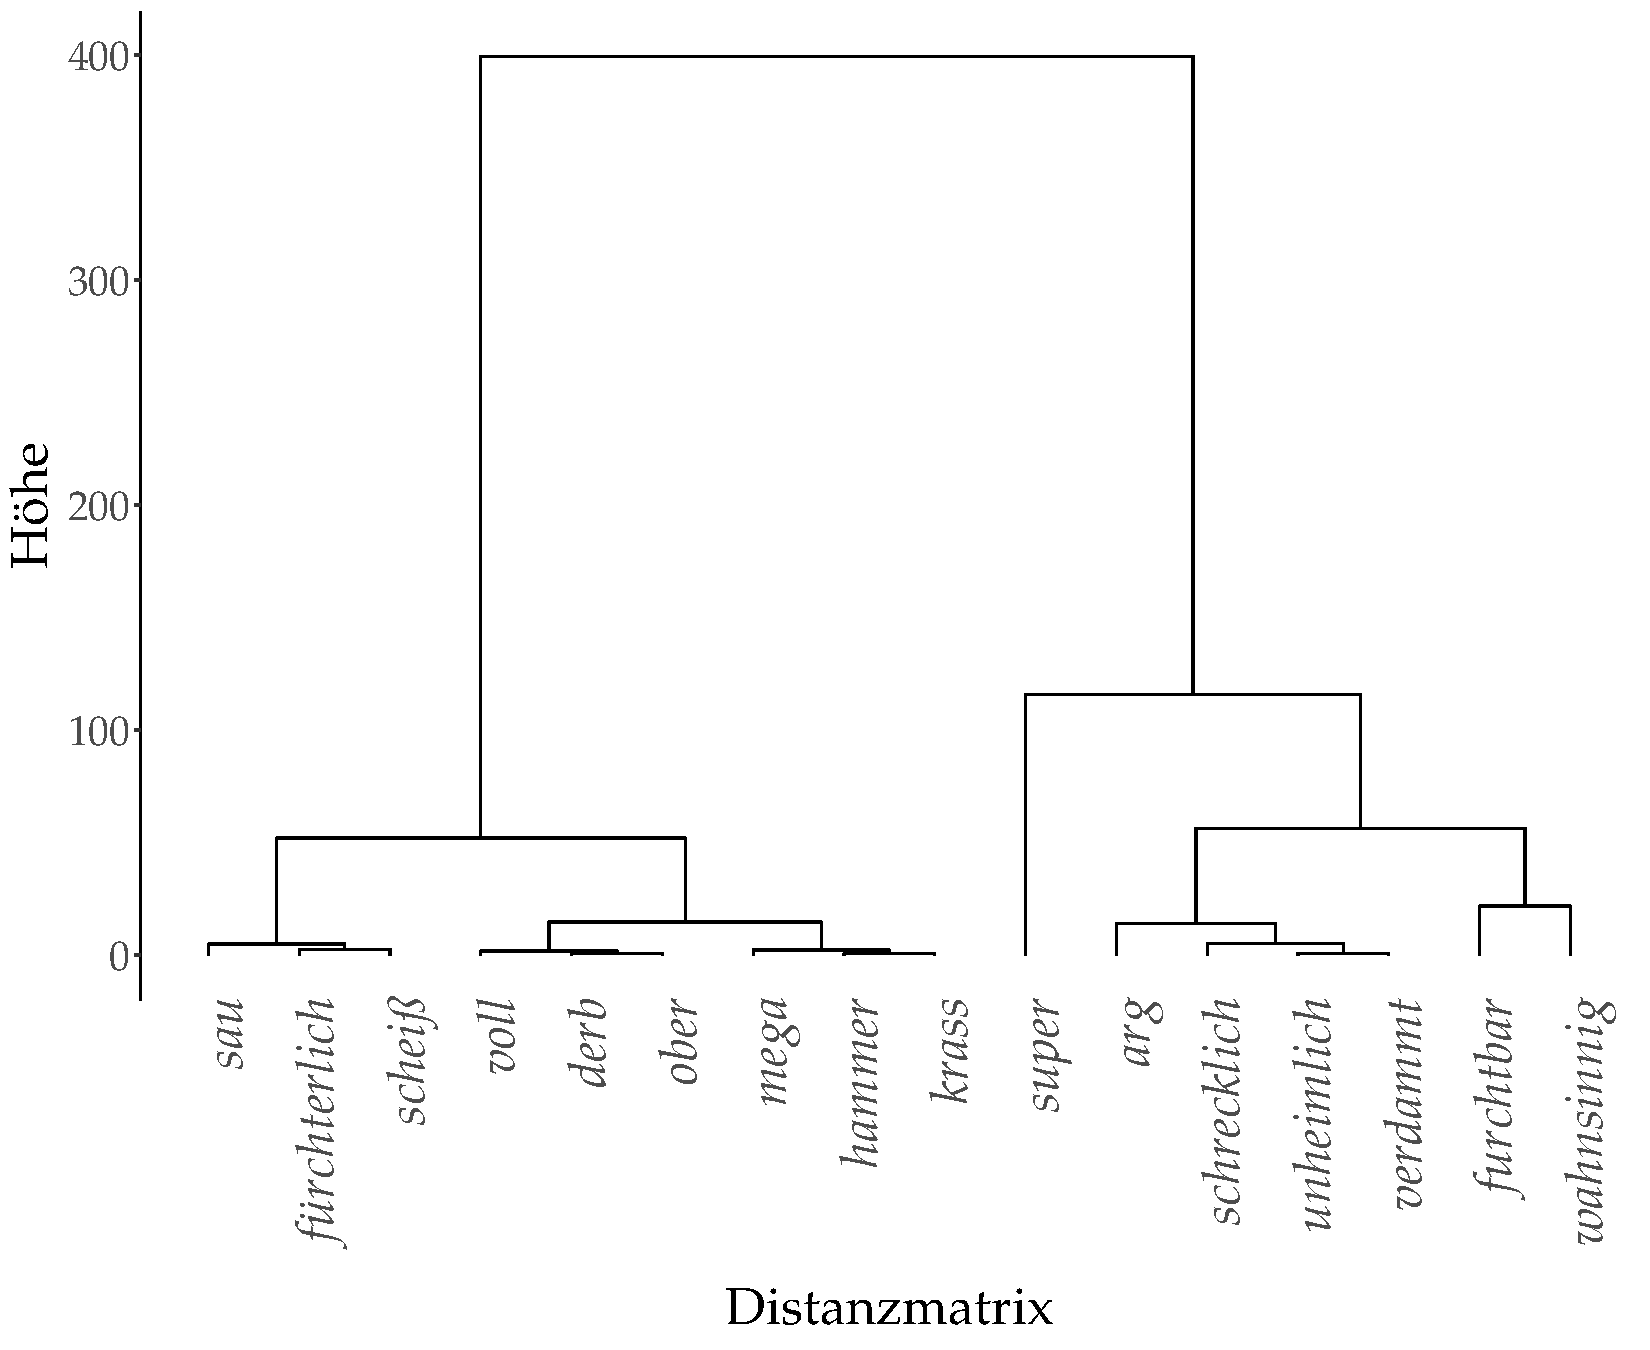
\includegraphics[width=1\textwidth]{1970-1989}
\caption[Cluster-Dendrogramm der expressiven Intensivierer für den Zeitraum von 1970 bis 1989]{Cluster-Dendrogramm der expressiven Intensivierer für den Zeitraum von 1970 bis 1989 (Maß: Euklidische Distanz; Amalgamierungsmethode: Ward-Verfahren (\citealt[]{Ward.1963})).}
\label{Dendro2}
\end{figure}

In \figref{Dendro2} ist das Dendrogramm für den Zeitabschnitt 1970 bis 1989 dargestellt. Dieses zerfällt erneut in zwei Cluster, die sich wiederum aus mehreren Subclustern zusammensetzen. Auch hier befinden sich im linken Cluster Ausdrücke mit niedriger Korpusfrequenz: \textit{sau}, \textit{fürchterlich}, \textit{scheiß}, \textit{voll}, \textit{derb}, \textit{ober}, \textit{mega}, \textit{hammer} und \textit{krass}. Die neuen Intensivierer \textit{mega}, \textit{hammer} und \textit{krass} sind aufgrund ähnlichen Vorkommens im Korpus in ein Subcluster zusammengefasst. Im Gegensatz dazu beinhaltet das zweite Cluster die frequenteren Ausdrücke und wird dementsprechend durch \textit{super}, \textit{arg}, \textit{schrecklich}, \textit{unheimlich}, \textit{verdammt}, \textit{furchtbar} und \textit{wahnsinnig} gebildet. Im Dendrogramm ist weiterhin der beschriebene Wechsel des vormals niedrigfrequenten Intensivierers \textit{wahnsinnig} in die hochfrequente Gruppe zu sehen, genauso wie sich darin die stärkere Frequenzzunahme von \textit{super} herauskristallisiert. Gleichwohl die \glqq{}schrecklichen\grqq{} Intensivierer  im Korpus vergleichsweise frequenter sind, hat sich das Vorkommen von \textit{super} in diesem Intervall sogar mehr als verdoppelt. Auch dieses Dendrogramm deutet auf ein Zutreffen der für den Zeitabschnitt von 1970 bis 1989 vorgenommenen Gruppeneinteilung hin, ohne dass Anpassungen vonnöten sind.

\subsubsection{Zeitabschnitt von 1990 bis 2017} \label{abs:Freqgruppe}
Wie schon im vorherigen Intervall sind auch im letzten alle 16 expressiven Intensivierer im Zeitschriftenkorpus vertreten. Diese lassen sich mit insgesamt 956,04 Treffern pro Million Textwörter nachweisen. Die Gruppe der niedrigfrequenten Ausdrücke setzt sich wiederholt aus \textit{derb}, \textit{krass}, \textit{hammer}, \textit{mega}, \textit{ober}, \textit{fürchterlich}, \textit{scheiß}, \textit{voll} und \textit{sau} (n = 9) zusammen. Diese Intensivierer kommen im Korpus mit maximal 37 Belegen vor (${\scriptstyle \sum{}}$ = 163,30). Erheblich häufiger sind dagegen die Intensivierer \textit{unheimlich}, \textit{arg}, \textit{schrecklich}, \textit{furchtbar}, \textit{wahnsinnig}, \textit{verdammt} und \textit{super} (n = 7) zu finden, die auch in diesem Zeitabschnitt die Gruppe der hochfrequenten Intensivierer bilden (${\scriptstyle \sum{}}$ = 792,74) und im Korpus mit mindestens 72 Treffern nachweisbar sind. Die beiden Frequenzgruppen sind inklusive der kumulierten Häufigkeiten ihrer Mitglieder in Tabelle \ref{Fre3.1} detailliert aufgeschlüsselt. Die Sortierung der Gruppenmitglieder erfolgt in zunehmender Frequenz.

\begin{table}
\begin{tabularx}{\textwidth}{l@{}>{\raggedleft}p{2cm}@{}>{\raggedleft}p{2cm}@{}>{\raggedleft}p{2.5cm}@{~}r@{}Y}
\lsptoprule
{Intensivierer} & {Absolute}  Frequenz& {Relative} Frequenz& {Prozentualer} Anteil& & {Klassifikation} \\
\midrule
\textit{derb}  & {42} & {4,35}	&	{0,46\,\%}	& \rdelim\}{9}{.3cm} &  \\
\textit{krass} & {72} &	{7,01}	&{0,73\,\%}	& 			&\\
\textit{hammer} & {77} &	{7,58}&		{0,79\,\%}& &\\
\textit{mega} & {113} &	{11,19}	&	{1,17\,\%}& &  \multirow{3}{*}{\parbox{2.5cm}{{niedrigfrequent \\ (17,09\,\%)}}}  \\
\textit{ober} & {147} &	{14,69}	&	{1,54\,\%}& &  \\
\textit{fürchterlich} & {238} & {23,36}&	{2,44\,\%}		& &  \\
\textit{scheiß} & {273} & 	{27,08}&	{2,83\,\%}	& &\\
\textit{voll} & {319} & {31,82}	&	{3,33\,\%}& &\\
\textit{sau} & {353} & {36,22}&	{3,79\,\%} & & \\
\midrule
\textit{unheimlich} & {717} & {71,97}& {7,53\,\%} & \rdelim\}{7}{.3cm} & \\
\textit{arg} & {801} & {80,44}& {8,41\,\%} & &\\
\textit{schrecklich} & {898} & {89,06}& {9,32\,\%} & & \multirow{3}{*}{\parbox{2.5cm}{{hochfrequent \\ (82,91\,\%)}}}\\
\textit{furchtbar} & {981} & {96,39}& {10,08\,\%} & & \\
\textit{wahnsinnig} &  {1\,083} & {104,53}& {10,93\,\%}& &     \\
\textit{verdammt} & {1\,365} &  {137,22}&{14,35\,\%} & &\\
\textit{super} & {2\,138} & {213,13}&{22,29\,\%}  & & \\
\bottomrule   %82,91\\
In Summe & {9\,617} & {956,04} & {100\,\%} & &\\
\lspbottomrule
\end{tabularx}

\caption[Kumulierte Häufigkeitsverteilungen der expressiven Intensivierer im Zeitraum von 1990 bis 2017]{Kumulierte Häufigkeitsverteilungen der expressiven Intensivierer im Zeitraum von 1990 bis 2017 (angeordnet nach zunehmender Frequenz).}
\label{Fre3.1}
\end{table}

%%%%%%%%%%%%%%%%%%

\noindent In diesem Zeitraum weist \textit{unheimlich} im Vergleich zu \textit{sau} nahezu doppelt so viele Treffer auf, was für eine Grenze zwischen diesen beiden Ausdrücken spricht. Ebenso haben in diesem Intervall die rezent etablierten Intensivierer \textit{krass}, \textit{mega} und \textit{hammer} an Frequenz dazugewonnen und den älteren Ausdruck \textit{derb} hinter sich gelassen. Im Hinblick auf die Gruppenzusammensetzung zeigt sich verhältnismäßig wenig Veränderung. So gliedert sich die Gruppe der hochfrequenten Intensivierer noch immer vorwiegend in die negativ konnotierten Ausdrücke mit transparenter Quellsemantik. Lediglich \textit{super} stellt in diesem Punkt eine Ausnahme dar, stammt der Ausdruck doch aus dem Lateinischen und gibt qua Semantik an, dass eine kontextuell festgelegte Norm überschritten wird. Die kumulierten Frequenzen demonstrieren darüber hinaus, dass in diesem Zeitabschnitt ebenfalls die beiden Intensivierer \textit{wahnsinnig} und \textit{verdammt} den Wert von 100 Belegen überschritten haben, wohingegen \textit{super} seinen Vorsprung sogar auf über 200 Treffer pro Million Textwörter verdoppelt hat. Somit ist der Ausdruck auch im dritten Intervall der im Korpus am häufigsten vorkommende Intensivierer.

\figref{Dendro3} illustriert das Dendrogramm für die Zeit von 1990 bis 2017.

\begin{figure}

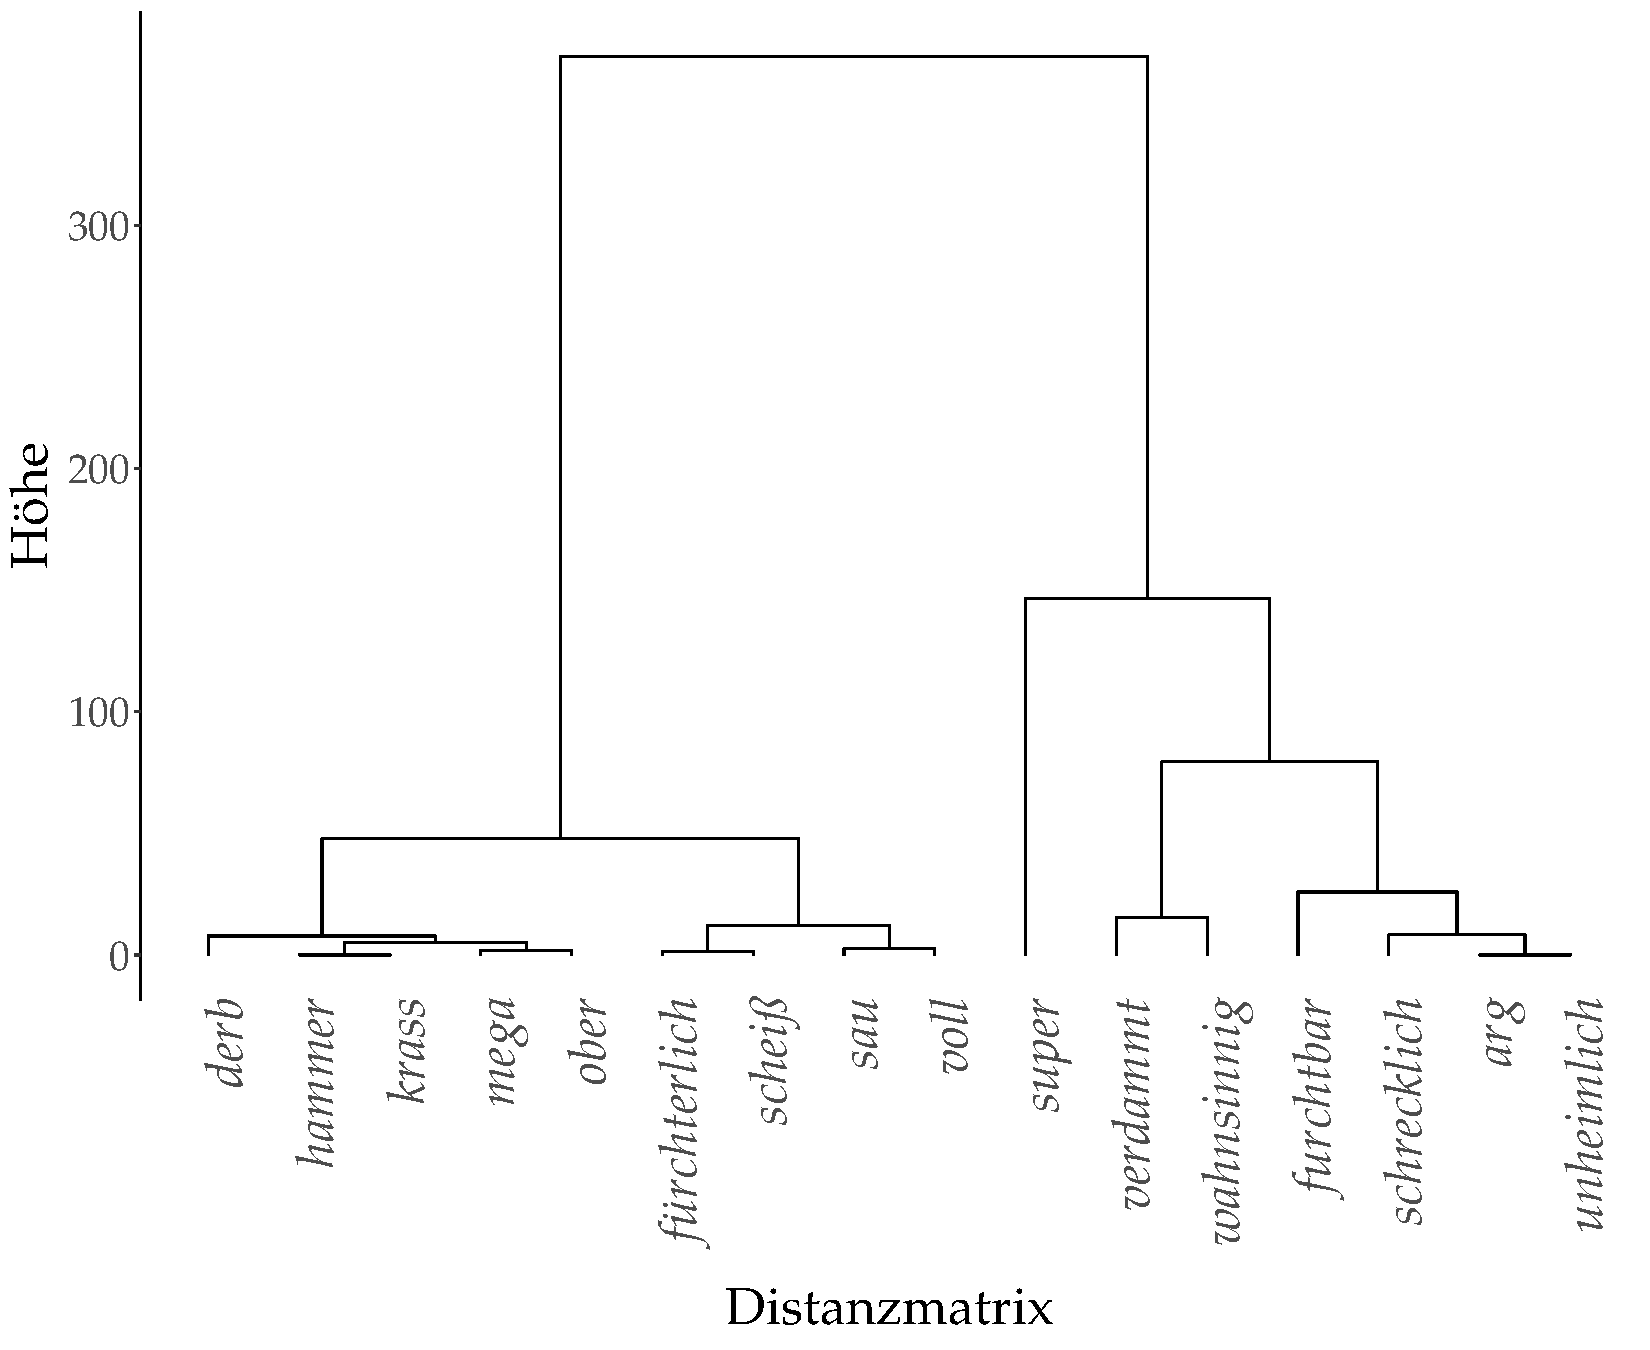
\includegraphics[width=1\textwidth]{1990-2017}
\caption[Cluster-Dendrogramm der expressiven Intensivierer für den Zeitraum von 1990 bis 2017]{Cluster-Dendrogramm der expressiven Intensivierer für den Zeitraum von 1990 bis 2017 (Maß: Euklidische Distanz; Amalgamierungsmethode: Ward-Verfahren (\citealt[]{Ward.1963})).}\label{Dendro3}
\end{figure}

\noindent Wie die vorigen setzt sich das letzte Dendrogramm aus zwei Clustern mit mehreren Subclustern zusammen. Das Cluster, das die niedrigfrequenten Intensivierer beinhaltet, zerfällt erwartungsgemäß in \textit{derb}, \textit{hammer}, \textit{krass}, \textit{mega}, \textit{ober}, \textit{fürchterlich}, \textit{scheiß}, \textit{sau} und \textit{voll}. In Bezug auf seine Häufigkeit unterscheidet sich \textit{derb} in diesem Zeitabschnitt erstmals stark von den restlichen niedrigfrequenten Ausdrücken. Außerdem haben auch die neuen Intensivierer sichtbare Entwicklungen durchlaufen: So bilden \textit{hammer} und \textit{krass} aufgrund ähnlicher Frequenzen ein Subcluster, während \textit{mega} zusammen mit \textit{ober} ein weiteres bildet. Demnach kommt es im dritten Intervall also erstmals zu einer Trennung der rezent in Erscheinung getretenen Ausdrücke, deren Ursache in den unterschiedlichen Frequenzverläufen liegt. Noch ausgeprägter sind die Unterschiede im zweiten Cluster, das die hochfrequenten Intensivierer \textit{super}, \textit{verdammt}, \textit{wahnsinnig}, \textit{furchtbar}, \textit{schrecklich}, \textit{arg} und \textit{unheimlich} umfasst. Obwohl sich bezüglich der Gruppenzusammensetzung im Vergleich zum vorherigen Zeitabschnitt per se keine Veränderungen ergeben haben, sind die Unterschiede zwischen den Subclustern hingegen erheblich markanter. Diese lassen sich auf die Zunahme der Korpusfrequenzen zurückführen, die eine klarere Ausdifferenzierung der Subgruppen nach sich zieht. Die Zusammensetzung der Subcluster unterscheidet sich dabei in dem Sinne von der des vorangegangenen Intervalls, dass in diesem Zeitraum neue frequenzbedingte Intensiviererpaare auszumachen sind, bspw. die beiden hochfrequenten Intensivierer \textit{arg} und \textit{unheimlich}. Noch auffälliger ist die Entwicklung, die \textit{super} vom zweiten zum dritten Zeitabschnitt durchlaufen hat: Wies es im zweiten Intervall noch ca. 122 Korpusbelege auf, so ist sein Gebrauch im dritten auf über 200 Treffer pro Million Textwörter angestiegen. Im Dendrogramm resultiert diese Entwicklung in einem ausgeprägteren Unterschied zwischen \textit{super} und der Gruppe der \glqq{}schrecklichen\grqq{} Intensivierer, der sich vom ersten bis zum dritten Zeitraum sukzessive gesteigert hat. Kurz gefasst deutet auch dieses Dendrogramm auf ein Zutreffen der für das Intervall von 1990 bis 2017 angenommenen Gruppeneinteilung hin, ohne dass Anpassungen vorzunehmen sind.

\subsubsection{Direkter Vergleich der Zeitabschnitte}
Nachdem die festgelegten Intervalle der Reihe nach analysiert wurden, folgt in diesem Abschnitt ein direkter Vergleich ebendieser, der sich nach den für die Hypothese H1 zentralen Faktoren Erstvorkommen (vgl. H1-Temp) und Frequenz (vgl. H1-Freq) richtet. Um einen besseren Überblick über die Gegenüberstellung zu geben, werden die kumulierten Häufigkeiten der Intensivierer pro Zeitraum inklusive ihrer prozentualen Entwicklungstendenz in Tabelle \ref{Fre4} komprimiert dargelegt. Diese  Werte sind in zunehmender Gesamtfrequenz gelistet. In der Tabelle sind jeweils diejenigen Spalten farblich hervorgehoben, bei denen sich eine diachrone Frequenzabnahme abzeichnet. Wie zu Beginn des Kapitels beschrieben, ist im Sinne der in Abschnitt \ref{Auslöser} umrissenen Expressivitätsmaximen nach \citet[]{Kirschbaum.2002b} davon auszugehen, dass eine rückläufige Entwicklung von Ausdrücken entscheidende Anhaltspunkte für den zur Diskussion stehenden Expressivitätsverlust bietet.

\begin{table}
\small
\begin{tabularx}{\textwidth}{l@{} YY YY YY}
\lsptoprule
{Intensivierer}  & \multicolumn{5}{c}{\textbf{Relative Frequenz}} & {Summe} \\
\cmidrule{2-6}
& 1950--1969 & Tendenz (in \%) & 1970--1989 & Tendenz (in \%) & 1990--2017 & \\
\midrule \\
\textit{krass} & -- & -- & 0,10 & +6\,910,00 & 7,01 & {7,10} \\
\textit{hammer} & -- & -- & 0,12 & +6\,216,67 & 7,58 & {7,69} \\
\textit{mega} & -- & -- & 0,24 & +4\,562,50 & 11,19 & {11,43} \\
\textit{ober} & \cellcolor[gray]{0.75} 3,01 & \cellcolor[gray]{0.75} - 5,98 & \cellcolor[gray]{0.75} 2,83 & +412,72 & 14,69 & {20,53} \\
\textit{derb}  & \cellcolor[gray]{0.75} 11,71 & \cellcolor[gray]{0.75} - 48,76  & \cellcolor[gray]{0.75} 6,00 & \cellcolor[gray]{0.75} - 27,50 & \cellcolor[gray]{0.75} 4,35 & {22,07} \\
\textit{voll} & 1,68 & +87,50 & 3,15 & +910,16 & 31,82 & {36,65} \\
\textit{scheiß} & 1,18 & +1\,061,86 & 13,71 & +97,52 & 27,08 & {41,96} \\
\textit{fürchterlich} & 6,27 & +120,89 & 13,85 & +68,66 & 23,36 & {43,49} \\
\textit{sau} & 10,78 & +24,40 & 13,41 & +170,10 & 36,22 & {60,41}  \\
\midrule
\textit{wahnsinnig} & 6,90 & +278,99 & 26,15 & +299,73 & 104,53 & {137,58} \\
\textit{unheimlich} & 25,69 & +150,02 & 64,23 & +12,05 & 71,97 & {161,89} \\
\textit{furchtbar} & 35,73 & +25,92 & 44,99 & +114,25 & 96,39 & {177,10} \\
\textit{arg} & 38,21 & +74,95 & 66,85 & +20,33 & 80,44 & {185,50} \\
\textit{schrecklich} & 40,65 & +39,11 & 56,55 & +57,49 & 89,06 & {186,26} \\
\textit{verdammt} & 39,94 & +28,34 & 51,26 & +167,69 & 137,22 & {228,42} \\
\textit{super} & 56,01 & +118,03 & 122,12 & +74,53 & 213,13 & {391,26}\\
\midrule
In Summe & 277,76 & +74,81 & 485,56 & +96,86 & 956,04    	& 1\,719,36\\
\lspbottomrule
\end{tabularx}
\caption[Kumulierte Häufigkeitsverteilungen der expressiven Intensivierer im Zeitraum von 1950 bis 2017]{Kumulierte Häufigkeitsverteilungen der expressiven Intensivierer im Zeitraum von 1950 bis 2017 (in zunehmender Frequenz).}
\label{Fre4}
\end{table}

%%%%%%%%%%%%%%%%%

\noindent Bei der Betrachtung von Tabelle \ref{Fre4} stellt sich heraus, dass beinahe alle der untersuchten Intensivierer trotz möglicher Schwankungen im Korpus häufiger im Gebrauch sind als zu Beginn des Untersuchungszeitraums. So sind einzig zwei Ausnahmen auszumachen, deren Frequenz prozentual betrachtet (zumindest temporär) schwindet. Dabei handelt es sich einerseits um \textit{derb}, bei dem quantitativ sowohl vom ersten zum zweiten Intervall als auch vom zweiten zum dritten Intervall eine starke Abnahme zu verzeichnen ist. Bei einem Vergleich des ersten Zeitraums mit dem dritten ist bei \textit{derb} insgesamt eine negative Differenz von -\,62,85\,\% zu konstatieren. Andererseits fällt ebenso der Gebrauch von \textit{ober} zeitweise marginal ab: Bei diesem Ausdruck ist eine leicht negative Differenz von -\,5,98\,\% vom ersten zum zweiten Zeitabschnitt zu erkennen. Diese Einbuße gleicht sich vom zweiten zum dritten Intervall allerdings insofern wieder aus, als die Frequenz von \textit{ober} in den beiden Zeitschriften verstärkt zunimmt. Alles in allem steigt die kumulierte Häufigkeit aller Ausdrücke vom ersten zum dritten Zeitabschnitt um 244,13\,\% an, was im Einklang mit den in \figref{Dia-rest} dargestellten diachronen Häufigkeitsverteilungen steht. Demnach haben die expressiven Intensivierer über den Untersuchungszeitraum hinweg stark an Frequenz dazugewonnen.

Als Nächstes wird eine paarweise Begutachtung der Zeitabschnitte vorgenommen. Dadurch kann überprüft werden, wie sich die expressiven Intensivierer relativ zu den Intervallen verhalten und welche Entwicklungstendenzen daraus abgeleitet werden können. Begonnen wird mit einer Gegenüberstellung des ersten Zeitraums (d.\,h. von 1950 bis 1969) mit dem zweiten Zeitraum (d.\,h. von 1970 bis 1989), woraufhin der zweite Zeitraum mit dem dritten Zeitraum (d.\,h. von 1990 bis 2017) kontrastiert wird. Im Anschluss daran wird der Einteilung der beiden Frequenzgruppen genauer auf den Grund gegangen. Vor diesem Hintergrund ergibt sich die Frage, ob die untersuchten Ausdrücke in allen drei Zeitabschnitten derselben Frequenzgruppe angehören oder von der einen Frequenzgruppe in die andere übertreten. Um diese zu beantworten, sind die Ausdrücke gemäß dieser Einteilung in Tabelle \ref{tab:Freqgruppe} aufgeführt. Darin wird zunächst jeder Zeitabschnitt separat berücksichtigt (d.\,h. 1950 bis 1969, 1970 bis 1989 sowie 1990 bis 2017), woraus für jeden Ausdruck letztlich eine Gesamttendenz abgeleitet wird.

\subsubsubsection{\textbf{1950--1969} vs. \textbf{1970--1989}}

Der markanteste Unterschied zwischen dem ersten und zweiten Zeitabschnitt besteht darin, dass im ersten noch nicht alle der untersuchten Intensivierer im Korpus ausgebildet sind. So lassen sich in diesem Intervall bloß 13 Ausdrücke nachweisen, tauchen \textit{hammer}, \textit{krass} und \textit{mega} doch erst im zweiten Intervall zum ersten Mal auf. Diese treten dann zunächst einmal in nur geringer Frequenz auf, was sich in Tabelle \ref{Fre4} naturgemäß in einer übermäßig stark ausgeprägten Anstiegskurve niederschlägt. Demnach handelt es sich bei \textit{hammer}, \textit{krass} und \textit{mega} um Ausdrücke, die erst im Laufe des Untersuchungszeitraums im Korpus neu dazukommen sind. Was die Mitglieder der beiden Frequenzgruppen anbelangt, gibt es mit Ausnahme der rezent etablierten Intensivierer keine bemerkenswerten Veränderungen. Lediglich \textit{wahnsinnig} kommt im zweiten Zeitabschnitt vergleichsweise vier Mal so häufig im Korpus vor, wodurch es von der Gruppe der niedrigfrequenten in die der hochfrequenten Ausdrücke übergetreten ist. Durch diese Entwicklung hat die \glqq{}schreckliche\grqq{} Intensivierergruppe in diesem Intervall zugleich ein ebenso negativ konnotiertes Mitglied dazugewonnen, was zu einem Ausbau ebendieser führt. Daneben ist auffällig, dass \textit{fürchterlich} seine Frequenz im zweiten Intervall nicht nur verdoppelt hat, sondern auch an die Spitze der niedrigfrequenten Gruppe gestiegen ist. Andere Intensivierer dieses Clusters weisen dagegen einen bedeutend geringeren Zuwachs auf, wie z.\,B. bei \textit{sau} oder \textit{voll} zu sehen ist. Auf der Spitzenposition der Gruppe der hochfrequenten Intensivierer steht sowohl im ersten wie auch im zweiten Intervall \textit{super}, das sein Vorkommen stark ausgebaut hat und bereits zu dieser Zeit im Korpus mit über 100 Belegen nachgewiesen werden kann. Darüber hinaus finden sich mit \textit{arg}, \textit{furchtbar}, \textit{schrecklich}, \textit{unheimlich} und \textit{verdammt} Ausdrücke mit klar negativer Quellsemantik, die im zweiten Zeitabschnitt, wie soeben erwähnt, durch \textit{wahnsinnig} ergänzt werden. Diese hochfrequenten Intensivierer befinden sich beim Übergang vom ersten zum zweiten Intervall quantitativ im Anstieg, wenn auch nicht dergestalt, dass sie an den Wert von \textit{super} heranreichen. Haben sich die kumulierten Frequenzen der hochfrequenten Intensivierer durch die stark positive Entwicklung von \textit{super} sogar verdoppelt, sind die der niedrigfrequenten vom ersten zum zweiten Intervall kaum merklich angestiegen. Bei der Betrachtung der Häufigkeiten aller Ausdrücke ist ein starker Anstieg von mehr als 70\,\% auszumachen, was ein Indiz für eine dem Anschein nach unproblematischere Verwendung von expressiven Intensivierern in den Zeitschriften zu sein scheint.

\subsubsubsection{\textbf{1970--1989} vs. \textbf{1990--2017}}

Bei der Gegenüberstellung des zweiten Intervalls mit dem dritten ist besonders auffällig, dass die rezent aufgetretenen Intensivierer \textit{krass}, \textit{hammer} und \textit{mega} im letzten Zeitabschnitt über eine höhere Frequenz als \textit{derb} verfügen. Letzterer ist der einzige Ausdruck, dessen Entwicklung über den Untersuchungszeitraum hinweg konstant rückläufig war. Zu beobachten ist außerdem, dass die Mitglieder der Frequenzgruppen in beiden Intervallen gleich geblieben sind und sich bloß die häufigkeitsbedingte Anordnung und dadurch auch die Subgruppierung im Dendrogramm geändert hat. So ist z.\,B. der einstige Spitzenreiter \textit{fürchterlich} trotz geringer Frequenzzunahme im dritten Zeitabschnitt von \textit{scheiß}, \textit{voll} und \textit{sau} überholt worden, deren Häufigkeiten sich in diesem Intervall zum Teil sehr stark ausgebaut haben. Die niedrigfrequente Gruppe zeigt im Hinblick auf die kumulierten Häufigkeiten eine positive Entwicklung beim Übergang vom zweiten zum dritten Intervall. Diese zeigt sich in der Form, dass die Spitzenreiter \textit{voll} und \textit{sau} über 30 Korpustreffer aufweisen, sodass sich der Frequenzwert von ca. 14 Belegen vom zweiten Zeitabschnitt im dritten mehr als verdoppelt hat. Auch in der Gruppe der hochfrequenten Intensivierer treten derart markante Veränderungen auf. In dieser steht \textit{super} nach wie vor unangefochten an erster Stelle, während sich seine einstige Trefferzahl im dritten Intervall sogar auf über 200 Belege erhöht hat. Zudem finden sich mit \textit{wahnsinnig} und \textit{verdammt} zwei weitere Intensivierer, die mit über 100 Treffern pro Million Textwörter im Korpus nachgewiesen werden können. Bemerkenswert ist, dass die Frequenz vom ersten bzw. zweiten zum dritten Intervall stark zugenommen hat. So hat sich \textit{wahnsinnig} vom einstigen niedrigfrequenten Intensivierer im ersten Zeitabschnitt zu einem der höchstfrequenten Intensivierer im dritten Zeitabschnitt entwickelt, wohingegen sich ebenso die Frequenz von \textit{verdammt} im dritten Intervall mehr als verdoppelt hat. Demzufolge ist auch in diesem Cluster ein übermäßig ausgeprägter Anstieg der Ausdrücke zu verzeichnen, was eine stark positive Entwicklung in den kumulierten Häufigkeiten aller Intensivierer nach sich zieht. Die Gesamtfrequenz der expressiven Intensivierer hat sich beim Übergang vom zweiten zum dritten Intervall ebenfalls nahezu dupliziert. Infolgedessen sind letztlich mehr als doppelt so viele Intensivierer im Zeitschriftenkorpus enthalten wie zu Beginn des Untersuchungszeitraums. Dies ist auch mithilfe des in \figref{Dia-rest} dargestellten Säulendiagramms zu beobachten (vgl. erster und letzter Balken).

Neben den kumulierten Häufigkeiten werden die expressiven Intensivierer, wie oben angekündigt, mit Blick auf die beiden Frequenzgruppen `Niedrigfrequent' und `Hochfrequent' begutachtet. Tabelle \ref{tab:Freqgruppe} gibt einen Überblick über die Mitglieder der Frequenzgruppen je Zeitabschnitt und leitet auf dieser Grundlage für jeden Intensivierer eine Gesamttendenz ab. Die Sortierung der Ausdrücke erfolgt in ansteigender Frequenz. In der Tabelle ist jeweils diejenige Spalte farblich hervorgehoben, bei der ein Wechsel der Frequenzgruppe zu verzeichnen ist.

\begin{table}
\begin{tabularx}{\textwidth}{lXXXrl}
\lsptoprule
\multirow{3}{*}{Intensivierer} &  \multicolumn{3}{c}{\textbf{Frequenzgruppe}}  & & \multirow{3}{*}{Klassifikation}    \\
 & 1950--1969 & 1970--1989 & 1990--2017 &  &  \\
\midrule
\textit{hammer}  &  {--}	& {niedrig} & {niedrig}	& \rdelim\}{9}{.3cm} & \\
\textit{krass}  &  {--}	& {niedrig} & {niedrig}	&  &  \\
\textit{mega}  &  {--}	& {niedrig} & {niedrig}	&  &  \\
\textit{derb}  &  {niedrig}	& {niedrig} & {niedrig}	&  &   \\
\textit{fürchterlich}  & {niedrig}	& {niedrig} & {niedrig}	&  &   { {{niedrig   (n = 9)}}}  \\
\textit{ober}  &  {niedrig}& {niedrig} & {niedrig}	&  &  \\
\textit{sau}  & {niedrig}	& {niedrig} & {niedrig}	&  &  \\
\textit{scheiß}  & {niedrig}	& {niedrig} & {niedrig}	&  &  \\
\textit{voll}  & {niedrig}	& {niedrig} & {niedrig}	&  &  \\
\midrule
\shadecell  \textit{wahnsinnig}  & \shadecell   niedrig &   \shadecell   hoch  &   \shadecell   hoch 	& \rdelim\}{7}{.3cm}  &  \\
\textit{arg}  &  {hoch}	& {hoch} & {hoch}	& &  \\
\textit{furchtbar}  &  {hoch}	& {hoch} & {hoch}	& & \\
\textit{schrecklich}  &  {hoch}	& {hoch} & {hoch}	& &   { {{hoch   (n = 7)}}}  \\
\textit{super}  &  {hoch}	& {hoch} & {hoch}	& &  \\
\textit{unheimlich}  &  {hoch}	& {hoch} & {hoch}	& &  \\
\textit{verdammt}  &  {hoch}	& {hoch} & {hoch}	& &  \\
\midrule\\
\lspbottomrule
\end{tabularx}
\caption[Einteilung der expressiven Intensivierer nach Frequenz im Zeitraum von 1950 bis 2017]{Einteilung der expressiven Intensivierer nach Frequenz im Zeitraum von 1950 bis 2017 (angeordnet nach Frequenzgruppe).}
\label{tab:Freqgruppe}
\end{table}

Aus Tabelle \ref{tab:Freqgruppe} ist abzulesen, dass die meisten expressiven Intensivierer ihre Frequenzgruppe über den gesamten Untersuchungszeitraum beibehalten. So zeichnet sich bei 15 Intensivierern dahingehend ein konstantes Muster ab, wobei niedrig- und hochfrequente Ausdrücke gleichermaßen davon betroffen sind. Eine Sonderstellung nimmt \textit{wahnsinnig} ein, das beim Wechsel vom ersten zum zweiten Zeitabschnitt von der niedrigfrequenten Gruppe in die Gruppe der hochfrequenten Intensivierer übergetreten ist. Weil der Ausdruck im Korpus auch im dritten Intervall unverändert hochfrequent ist und sich die im zweiten Intervall ermittelte Häufigkeit von 26,15 Treffer pro Million Textwörter im dritten Intervall auf 104,53 Belege vervierfacht hat (vgl. die Tabellen \ref{Fre2} und \ref{Fre3.1}), ist seine Gesamttendenz ebenso als hoch einzuschätzen.

Zusammengenommen umfassen die Gruppen ingesamt neun niedrigfrequente und sieben hochfrequente Intensivierer. Lassen sich erstere in Summe mit 258,24 Treffern pro Million Textwörter nachweisen ($\hateq$ 15,02\,\%), sind letztere im Zeitschriftenkorpus mit 1461,12 Belegen vertreten ($\hateq$ 84,98\,\%).

\section{Diskussion} 		\label{DisKor}
\largerpage
Nachfolgend werden die im vorangegangenen Abschnitt dargelegten Ergebnisse der Korpusuntersuchung besprochen. Diese wurde mit dem Ziel durchgeführt, synchrone und diachrone Häufigkeitsverteilungen ausgewählter expressiver Intensivierer über einen umfassenden Zeitraum zu erheben, um einigen in der Literatur vertretenen Annahmen zum ersten Mal empirisch nachzugehen. So ist im Sinne der Hypothese H1-Freq nach \citet[2]{Hauschild.1899} davon auszugehen, dass Intensivierer infolge von inflationärem Gebrauch ihre Expressivität verlieren und in der Konsequenz seltener verwendet werden. Nach \citet[59]{Tobler.1868} spielt dabei auch der Faktor Zeit eine Rolle, der in der Hypothese H1-Temp berücksichtigt wurde. Um den Ausfall abgenutzter Intensivierer zu kompensieren, bedarf es \citet[274]{Baumgarten.1908} zufolge permanent neuer expressiver Ausdrücke. Diese Aussage wurde im Rahmen der Hypothese H2 auf ihre Gültigkeit hin überprüft.

Nachdem im Folgenden zunächst auf den deskriptiven Intensivierer \textit{sehr} eingegangen wird, folgt daraufhin eine Begutachtung der expressiven Intensivierer unter Bezugnahme der Ergebnisse der hierarchischen Clusteranalyse. Abschließend werden die gewonnenen Resultate zusammengefasst und in Hinsicht auf die soeben umrissenen Hypothesen evaluiert.

\subsection{Deskriptiver Intensivierer}

Anhand der Ergebnisse der Korpusanalyse lässt sich die longitudinale Entwicklung von \textit{sehr} als eine Delle mit fallendem Beginn und steigendem Ende beschreiben (vgl. \figref{Dia-sehr}), was einem diachronen Jo-Jo-Effekt entspricht. Der Tiefpunkt, der sich beim deskriptiven Intensivierer im Zeitraum von 1970 bis 1990 detektieren lässt, ist also überwunden. Durch Extrapolation ist anzunehmen, dass die Frequenzzunahme weiter andauert und das Gebrauchsmaximum noch nicht erreicht ist -- vorausgesetzt, die zuletzt beobachteten Häufigkeiten von \textit{sehr} bleiben in den darauffolgenden Jahren erhalten. Mit 20\,278,12 Belegen pro Million Textwörter ist \textit{sehr}, wie prognostiziert, der mit Abstand am meisten verwendete Intensivierer im Korpus. Dieses Ergebnis deckt sich mit der Beobachtung, die \citet[266]{Ito.2003} im Rahmen ihrer Korpusuntersuchung in Bezug auf das englische Pendant \textit{very} machten. Auch legt es die Vermutung nahe, dass \textit{sehr} unangefochten der häufigste Intensivierer im Deutschen ist. Somit besteht offensichtlich keine Gefahr eines dauerhaften Rückgangs oder gar einer Verdrängung durch andere Intensivierer. Angesichts der anfangs zu verzeichnenden Frequenzabnahme von \textit{sehr} lässt sich einerseits spekulieren, dass es sich dabei um ein Artefakt der Daten handelt, das nicht signifikant ist und aus linguistischer Sicht keine Relevanz hat. Andererseits können ebenfalls die gesellschaftlichen Rahmenbedingungen als Erklärung in Betracht gezogen werden. So ist z.\,B. denkbar, dass der Schreibstil in den Zeitschriften in der Nachkriegszeit nüchterner ausfiel, die Journalist:innen neutralere Berichterstattung leisteten und der Ausdruck einer allgemeinen Tendenz zur Vermeidung von Intensivierern unterlag. Dementsprechend könnte die Ursache für den zeitweisen Schwund extralinguistisch durch soziokulturelle Faktoren bedingt sein. Auch wenn bezüglich des Rückgangs an dieser Stelle lediglich Spekulationen möglich sind, deutet der Anstieg, der sich ab den Neunzigerjahren abzeichnet, auf eine weiterhin starke Verwendung ohne Abnutzungserscheinungen hin. Diese ist abgesehen vom hohen Lexikalisierungsgrad vor allem der skalaren Bedeutung geschuldet, die \textit{sehr} zum klassischen Intensivierer des Standarddeutschen macht. Im Hinblick auf die eher konservativen Textsorten, aus denen sich das Untersuchungskorpus zusammensetzt, bietet \textit{sehr} die neutralste Möglichkeit zur Skalierung, die auch in Printmedien angemessen ist. So handelt es sich bei Zeitungen nach \citet[]{Koch.1996,Koch.2007} um eine konzeptionell schriftliche Kommunikationsform, die deutlich stärker zu einem deskriptiven als expressiven Stil neigt. Dies konnte durch die Untersuchung gezeigt werden. Dagegen gilt die expressive Intensivierung gemeinhin als mündlichkeitsnahes Phänomen, das, ähnlich wie andere Formen von Expressivität (z.\,B. Modalpartikeln), in der Schriftsprache eher zu vermeiden ist \citep[vgl.][9]{Weydt.1969}. Obwohl der Gebrauch von \textit{sehr} nach einer temporären Einbuße aus den genannten Gründen (d.\,h. stilistisch wenig stigmatisierte Verwendung durch Delexikalisierung, hoher Lexikalisierungsgrad und fehlende Expressivität) im Korpus zwar wieder zugenommen hat, ist dennoch vorstellbar, dass es in der mündlichen Kommunikation nicht ausdrucksstark genug ist. Infolgedessen ist gemäß den in Abschnitt \ref{Auslöser} dargelegten Expressivitätsmaximen nach \citet[]{Kirschbaum.2002a} in mündlichkeitsnahen Sprachdomänen zu erwarten, dass expressive Intensivierer gegenüber deskriptiven Intensivierern präferiert verwendet werden, wenn zusätzlich zur Graduierung auch subjektive Einstellungen bekundet werden sollen -- jedenfalls sofern die hierzu in der Literatur vorherrschende Annahme (vgl. bspw. \citealt[315]{Lang.1983}; \citealt[57]{Ortner.2014}) korrekt ist. Die noch bestehenden Unklarheiten und angeführten Mutmaßungen in Bezug auf die diachrone Entwicklung von \textit{sehr} können als theoretische Grundlage für weiterführende korpuslinguistische oder experimentelle Untersuchungen dienen.

\subsection{Expressive Intensivierer}

Im Anschluss werden die Ergebnisse der expressiven Intensivierer besprochen. Die Diskussion erfolgt zum einen auf Basis der festgestellten semantischen Ähnlichkeiten und zum anderen auf Basis der kumulierten Häufigkeiten unter Bezugnahme der Ergebnisse der hierarchischen Clusteranalyse.

Das erste augenscheinliche Resultat hinsichtlich der expressiven Intensivierer ist mithilfe des in \figref{Dia-rest} dargestellten Säulendiagramms zu erkennen. Dem darin veranschaulichten diachronen Verlauf folgend haben die expressiven Intensivierer stark an Frequenz dazugewonnen. So sind die in den ersten Intervallen verzeichneten Häufigkeiten bis zu den letzten linear und beinahe auf das Dreifache angestiegen. Wie an entsprechender Stelle ausgeführt, stellt dies insbesondere vor dem Hintergrund des zurate gezogenen Korpus ein unerwartetes Ergebnis dar. Somit hat nicht nur der Gebrauch des deskriptiven Intensivierers \textit{sehr} seit den Neunzigerjahren konstant zugenommen, sondern auch die expressiven Intensivierer zeigen ähnliche Entwicklungstendenzen an. Dies gibt erste Hinweise auf eine mögliche stilistische Veränderung der in den Zeitschriften verwendeten Schreibweise. Ebenso ist nicht ausgeschlossen, dass die diachronen Entwicklungen durch eine stärkere Gewichtung zugunsten meinungsäußernder Texte bzw. konzeptionell mündlich orientierter Textsorten wie Interviews, Leserbriefen oder Kommentaren begründet sind. Diese Annahme lässt sich allerdings aufgrund unzureichender Metadaten der Korpusdokumentation nicht belegen. Ungeachtet der Gründe ist die Frequenzzunahme unstrittig. Als Ergebnis kann folglich festgehalten werden, dass die Journalist:innen nach und nach vermehrt auf mündlichkeitsnahe Ausdrücke zurückgegriffen haben, was einen unkritischeren Gebrauch expressiver Intensivierer im Korpus nahelegt.

Zur Prüfung der Hypothesen H1-Temp und H1-Freq wurde der Untersuchungszeitraum in drei Abschnitte gegliedert, in denen die Häufigkeiten systematisch inspiziert wurden. Hier zeichneten sich recht früh erste Entwicklungstendenzen ab, die im Folgenden betrachtet werden. Begonnen wird mit den frequenten Intensivierern, allen voran \textit{super}. Dieser Ausdruck war von Beginn an am häufigsten im Korpus vertreten. Bis zum dritten Intervall hat sich seine Frequenz mit deutlicher Distanz zu den anderen Ausdrücken ausgebaut. Bei \textit{super} handelt es sich um einen Intensivierer lateinischen Ursprungs, der anzeigt, dass eine kontextuell determinierte Schwelle überschritten wird, sodass die beschriebene Eigenschaft eine \glqq{}Abweichung von der Normalität\grqq{} (\citealt[80]{Ruf.1996}) darstelle. Der Umstand, dass ausgerechnet der frequenteste Intensivierer ein Lehnwort ist, entkräftet überdies zu einem gewissen Grad die eingangs angeführte Hypothese von \citet[323]{Calpestrati.2017}, nach der deutsche Muttersprachler:innen in der Schriftsprache heimische Ausdrücke gegenüber entlehnten bevorzugen. Wenngleich dies auf die restlichen hochfrequenten Intensivierer durchaus zutrifft, stehen die Frequenzen von \textit{super} jedoch im Widerspruch dazu. In Bezug auf dessen Etymologie nach \citet[1398]{Pfeifer.1995} ist festzustellen, dass es sich bereits im 16. Jahrhundert als Intensivierer etabliert hat. Daher ist davon auszugehen, dass der Ausdruck einer der ältesten der untersuchten Intensivierer ist,\footnote{Ein weiteres Indiz für die lange Existenz des intensivierenden \textit{super} findet sich in \citet[109]{Tobler.1868}, der \textit{superklug} neben \textit{hyperkritik}, \textit{extrafein} und \textit{ultraradical} als Beispiel für eine \glqq{}moderne bildung\grqq{} nennt.} was als Erklärung für die verhältnismäßig hohe Korpusfrequenz in Erwägung gezogen werden kann. Interessanterweise deckt sich dieses Ergebnis mit den Resultaten, die \citet[345]{Ruf.1996} und \citet[104]{Androutsopoulos.1998} im Rahmen ihrer Korpusstudien erzielten: Auch bei ihnen trat \textit{super} mit Abstand am häufigsten im Korpus auf. \citet[345]{Ruf.1996} verweist in diesem Zusammenhang auf \citet[]{Wunderlich.1983}, der \textit{super} eine \glqq{}große Zukunft\grqq{} prophezeite. Dass der Anstieg bislang nicht abgeschlossen, das Frequenzmaximum noch nicht erreicht und der Intensivierer auch gegenwärtig von großer Relevanz ist, demonstrieren die Ergebnisse meiner Untersuchung ganz klar. Doch wie ist es um die Expressivität von \textit{super} bestellt? Dies lässt sich auf Basis der quantitativen Korpusdaten nicht abschätzen, sondern erfordert eine experimentelle Überprüfung. Eine solche vertiefende Einordnung wird in der in Kapitel \ref{Experiment0} vorgestellten experimentellen Untersuchung vorgenommen.

Ein gleichfalls markantes Ergebnis stellt die weitere Zusammensetzung des Clusters der hochfrequenten Ausdrücke dar, das neben \textit{super} schon von Beginn des Untersuchungszeitraums an \textit{unheimlich}, \textit{furchtbar}, \textit{arg}, \textit{verdammt} und \textit{schrecklich} beinhaltete. Zeigte dieses Cluster bereits im ersten Intervall eine Tendenz für Intensivierer mit klar negativer Semantik, wurde es ab dem zweiten Intervall zusätzlich durch \textit{wahnsinnig} unterstützt; einen Ausdruck, der ebenso einen negativen mentalen Zustand denotiert. Ähnlich wie \textit{super} bewegen sich diese Ausdrücke in einem hohen Frequenzbereich. Bei ihnen handelt es sich ausschließlich um transparente denominale bzw. deadjektivische Derivationen. Obwohl deren Semantik zwar erkennbar ist, ist sie in intensivierender Funktion der Einschätzung von \citet[15f.]{Nouwen.2020} zufolge jedoch gänzlich verblasst. Auch bei diesen Ausdrücken lässt sich die intensivierende Funktion mittels \mbox{\citet[385, 525, 1499]{Pfeifer.1995}} zeitlich früh verorten, d.\,h. zwischen dem 16. Jahrhundert (\textit{furchtbar}) und dem 19. Jahrhundert (\textit{unheimlich} und \textit{verdammt}). Demnach ist es naheliegend, dass die Intensivierer inzwischen über einen hohen Lexikalisierungsgrad verfügen und eine eher skalare Bedeutung angenommen haben. Dieser Punkt wird weiter unten unter dem Blickwinkel der Definition von Expressivitätsverlust erneut aufgegriffen und vertieft. Bei diesen Ausdrücken stellt sich also ebenfalls die Frage nach dem tatsächlichen Expressivitätsgrad. Vor dem Hintergrund der Kriterien Erstvorkommen (vgl. \mbox{H1-Temp}) und Frequenz (vgl. H1-Freq) ist anzunehmen, dass die hochfrequenten Intensivierer prinzipiell weniger expressiv sind als die niedrigfrequenten. Auch darüber kann die nachfolgend dargestellte experimentelle Untersuchung Aufschluss geben.

Wesentlich variabler ist dagegen die Zusammensetzung der Gruppe der niedrigfrequenten Intensivierer. Hier findet sich u.\,a. der einzige Ausdruck, der über die Zeit als Intensivierer sukzessive seltener gebraucht wurde, nämlich \textit{derb}. Dessen Verwendung ist seit dem Frequenzhöhepunkt Anfang der Sechzigerjahre weitgehend kontinuierlich zurückgegangen, was schließlich dazu führte, dass der Intensivierer im Korpus nahezu ausgestorben ist. Folglich stellt die beständige diachrone Frequenzeinbuße von \textit{derb} als Einziges ein hinreichendes Indiz für einen Verlust von Expressivität dar. Ob sich die Frequenzabnahme darauf zurückführen lässt, dass der Ausdruck infolge früherer häufiger oder persistenter Verwendung nach und nach an Expressivität verloren hat, oder ob er durch andere Intensivierer verdrängt wurde, weil er schlichtweg unbeliebter war, lässt sich korpuslinguistisch nicht überprüfen. In beiden Fällen könnte der für \textit{derb} nachteilige Status den Wandel zum Vorteil anderer Ausdrücke beschleunigt haben. Gemessen an den IpMW ist \textit{derb} neben dem vergleichsweise neuen Ausdruck \textit{krass} im letzten Zeitabschnitt (d.\,h. von 1990 bis 2017) der am seltensten verwendete Intensivierer. Auch die Betrachtung des ersten Intervalls (d.\,h. von 1950 bis 1969) bringt keine Indizien für einen hochfrequenten Gebrauch hervor. Damit bleibt die Frage bestehen, ob \textit{derb} in der Zeit vor 1950 häufiger (und unter Umständen zu häufig) verwendet wurde (vgl. H1-Freq). Diese muss in Anbetracht des beschränkten Untersuchungszeitraums allerdings unbeantwortet bleiben. Ähnliches trifft auf die Persistenz zu, die sich gleichermaßen als nachteilig für die Expressivität erweisen kann \mbox{(vgl. H1-Temp)}. Ungeachtet der tatsächlichen Gründe ist \textit{derb} auf den ersten Blick der einzige Intensivierer, dessen fortschreitender quantitativer Rückgang im Zeitschriftenkorpus zweifelsfrei auf einen Expressivitätsverlust hindeutet. Außerdem befinden sich in der Gruppe der niedrigfrequenten Ausdrücke diejenigen Intensivierer, die sich erst im Laufe der Zeit im Korpus neu etabliert haben und somit Evidenz für die Gültigkeit der Hypothese H2 nach \citet[274]{Baumgarten.1908} liefern, nämlich \textit{krass}, \textit{hammer} und \textit{mega}. Derzufolge gibt es einen ständigen Bedarf an neuen Intensivierern, um den Ausfall altgedienter Ausdrücke zu kompensieren. Darin sei zugleich die Hauptursache für die Wandelbarkeit des Inventars zu sehen, die dazu führt, dass Intensivierer in der Literatur als \glqq{}Modewörter\grqq{} (\citealt[267]{Becher.1907}) bezeichnet werden. Wie eingangs beschrieben, sollte sich das Zutreffen von H2 im Korpus durch die Herausbildung neuer Intensivierer ausdrücken. Dies legt die Entwicklung von \textit{krass}, \textit{hammer} und \textit{mega} nahe. Semantisch betrachtet entspricht letzterer Ausdruck der deutschen Präposition \textit{ober}, das ebenso in dieser Gruppe zu finden ist. Während \textit{mega} über das Griechische entlehnt wurde und nach \mbox{\citet[855]{Pfeifer.1995}} so viel wie `groß, hoch, lang, weit' bedeutet, trägt auch \textit{ober} eine dimensionale Bedeutung, die \mbox{\citet[940]{Pfeifer.1995}} mit `oben befindlich, höher gelegen, auf höherer Stufe stehend, übergeordnet' angibt. Daneben können \textit{hammer} und \textit{krass} im weiteren Sinne ebenso als verwandt angesehen werden: Der Hammer stellt als robustes Schlagwerkzeug einen starken, plumpen Gegenstand dar, der aufgrund seiner massiven physischen Kraft dazu dient, grobe Arbeiten zu verrichten. Ebendiese Adjektive, d.\,h. `dick, grob, derb, plump', bringt \citet[727]{Pfeifer.1995} mit der etymologischen Bedeutung von \textit{krass} in Verbindung, weshalb hier ebenfalls eine semantische Relation zu sehen ist. Bei \textit{fürchterlich}, \textit{scheiß} und \textit{sau} ist auffällig, dass es sich um Ausdrücke handelt, die sich ursprünglich von den polysemen, überwiegend negativ konnotierten Nomen abgeleitet haben: von der \textit{Sau} als weiblichem Schwein, der emotionalen Reaktion \textit{Furcht} sowie dem Fäkalwort \textit{Scheiße}. Insbesondere bei letzterem könnte die semantische Transparenz und die damit verbundene vulgäre Konnotation ausschlaggebend dafür sein, dass der Ausdruck im Zeitschriftenkorpus nicht häufiger vertreten ist. Ferner wird auch \textit{sau} in schriftsprachlichen Kontexten offenbar seit jeher als unangemessen betrachtet, tritt es nach \mbox{\citet[122]{Tobler.1868}} doch \glqq{}nur in der gemeinern sprache der mundarten\grqq{} auf. Auch existiert der Ausdruck seit dem Mittelhochdeutschen als Schimpfwort: \textit{Du blöde Sau} \mbox{\citep[vgl.][1168]{Pfeifer.1995}}.\footnote{Trotzdem berichtet \citet[270]{Becher.1907}, dass bei \textit{Schwein} und \textit{Sau} ehedem die Symbolik im Vordergrund gestanden habe, wurde das Tier in der Geschichte doch als heilig verehrt. Heute spielt hingegen wohl eher die damit verbundene negative Konnotation eine übergeordnete Rolle, durch die die Ausdrücke nahezu vorherbestimmt für die \mbox{Intensiviererrolle sind}.} Bei der Interpretation von Ausdrücke tierischen Ursprungs sieht \mbox{\citet[]{Claudi.2006}} primär die Gegensatzrelation Mensch vs. Tier bzw. Zivilisation vs. Natur vordergründig:

\begin{singlespace*}
\begin{quotation}
\noindent The intensifiers from the animal domain probably derived their intensifying power from a contrast humanity vs. non-humanity, or culture/civilisation vs. nature, where non-humanity or nature stands for everything that is uncontrolled, untamed, and instinctual. \hfill (\citealt[360]{Claudi.2006}) \\ \end{quotation}
\end{singlespace*}

Gleichfalls finden sich bei \textit{fürchterlich} und \textit{sau} in \mbox{\citet[386, 1168]{Pfeifer.1995}} Hinweise darauf, dass die Ausdrücke erstmals im 17. bzw. 19. Jahrhundert intensivierend aufgetreten sind. Das Erstvorkommen der anderen Intensivierer ist dagegen nicht belegt. Auf den ersten Blick ist es überraschend, dass \textit{fürchterlich} im Korpus nicht frequenter ist, steht es den Mitgliedern der \glqq{}schrecklichen\grqq{} Intensivierergruppe zumindest semantisch in Nichts nach. Nichtsdestotrotz handelt es sich bei vielen Intensivierern um morphologisch und phonologisch wenig komplexe Ausdrücke, die sich im Affekt schnell, unkompliziert und dennoch mit dem intendierten kommunikativ-pragmatischen Effekt artikulieren lassen. Vergleicht man bspw. die neuen Intensivierer \textit{krass} oder \textit{mega} mit den älteren wie \textit{unheimlich} oder \textit{wahnsinnig}, so zeichnet sich ein deutlicher Trend zur Kürze ab. Wie bereits erwähnt, sind die hohen Frequenzen der älteren Intensivierer vermutlich in erster Linie auf einen hohen Lexikalisierungsgrad zurückzuführen. Im Falle von \textit{fürchterlich} lässt sich an dieser Stelle mutmaßen, dass es zugunsten von \textit{furchtbar} als morphologisch und phonologisch einfacherer Variante (da weniger Silben und kein Umlaut) seltener gebraucht wurde. Zu guter Letzt fehlt noch \textit{scheiß}, bei dem 82,40\,\% der Treffer die weitgehend konventionalisierte Komposition \textit{scheißegal} (oder auch die Berliner Variante mit Phonemverschiebung von [ɡ] zu [j], d.\,h. \textit{scheißejal}) ausmachen, wohingegen lediglich 17,60\,\% auf andere Verbindungen zukommen. Daher ist zu erwägen, dass der Intensivierer \textit{scheiß} auf einige wenige Adjektive limitiert und gegebenenfalls nicht bloß im Korpus wenig produktiv ist. Bezüglich der Produktivität von niedrigfrequenten Ausdrücken erklärt \citet[72]{Kempf.2016}, dass eine \glqq{}sehr niedrige Tokenfrequenz einer Bildung darauf hindeuten [kann], dass es sich um eine Neubildung handelt.\grqq{} Meiner Ansicht nach ist dies bei \textit{scheiß} allerdings aus verschiedenen Gründen ausgeschlossen: Zum einen finden sich in meinem Korpus mit \textit{scheißfreundlich} und \textit{scheißnormal} schon im Zeitraum von 1958 bis 1960 erste Belege für das intensivierende \textit{scheiß}. Zum anderen hat sich sein Vorkommen über die Zeit allenfalls marginal verändert. Demnach ist der verhältnismäßig niedrige Gebrauch anderweitig begründet. So ist anzunehmen, dass die negative Konnotation des Ausdrucks in der Schriftsprache weniger angemessen ist als im mündlichen Sprachgebrauch, was dazu führt, dass \textit{scheiß} im Vergleich zu weniger offensiven Intensivierern seltener verwendet wird. Dass offensive, negativ konnotierte Ausdrücke wie \textit{scheiß} oder \textit{arsch} über eine derart geringe Korpusfrequenz verfügen, legt obendrein die Existenz eines semantischen Filters nahe. Dieser scheint in der Schriftsprache dafür zu sorgen, dass expressive Intensivierer mit negativem Herkunftsbereich und ebensolcher Konnotation schlechter Einzug in dieses Medium halten als Intensivierer, die opak oder abgenutzter, somit textsortenadäquater sind.

Auf Basis der Ergebnisse lässt sich zusammenfassen, dass die Häufigkeiten anscheinend zumindest partiell durch die Semantik der Ausdrücke zu erklären sind. Dieser Einfluss kann sowohl von Vorteil als auch von Nachteil sein: Während die semantische Transparenz die hohe Frequenz der \mbox{Mitglieder} der \glqq{}schrecklichen\grqq{} Intensivierergruppe womöglich begünstigt hat, hat sie sich bei anderen Intensivierern dagegen negativ ausgewirkt. Dies ist z.\,B. bei \textit{sau} und \textit{scheiß} zu beobachten, die sich im Korpus in nur geringer Zahl nachweisen lassen. Bei ihnen hat die Transparenz und die damit verbundene negative Konnotation den Gebrauch der Ausdrücke im Korpus offenbar behindert und dazu geführt, dass andere, weniger offensive Intensivierer bevorzugt verwendet wurden. So konstatiert bspw. \citet[311]{Calpestrati.2017}, dass der semantischen Konnotation eines Intensivierers eine tragende Rolle zukommt. Dies bestätigen auch die Ergebnisse meiner Korpusanalyse. Dennoch hebt \citet[229]{Pittner.1989} die Möglichkeit hervor, dass sich die mit einem Ausdruck verbundene Konnotation je nach Sprecher und Äußerungskontext verändern könne. So sei \textit{sau} für Erwachsene grundsätzlich stärker negativ konnotiert, wohingegen es für Jugendliche vielmehr mit etwas Positivem verbunden werde (\textit{sauteuer}, \textit{saudumm} vs. \textit{saugeil}, \textit{saustark}) \citep[vgl.][229]{Pittner.1989}. Ob diese dem Anschein nach introspektive Einschätzung (auch aus heutiger Sicht) der Realität entspricht, bedarf empirischer Überprüfung.

Doch was bedeuten die erbrachten Resultate für die zu testenden Hypothesen von \citet[2]{Hauschild.1899} und \citet[274]{Baumgarten.1908}, nach denen eine persistente und frequente Verwendung einen Verlust der Expressivität nach sich zieht (vgl. H1), woraus sich schließlich ein ständiger Bedarf an neuen Ausdrücken ergibt (vgl. H2)? Wie sich anhand der etwa 70-jährigen Entwicklung ablesen lässt, sind derzeit 15 der 16 ausgewerteten Intensivierer quantitativ im Anstieg. Dieser Anstieg bietet auf den ersten Blick zunächst einmal keine direkten Anhaltspunkte für einen Expressivitätsverlust. So ist vor dem Hintergrund der Expressivitätsmaximen nach \mbox{\citet[]{Kirschbaum.2002b}} anzunehmen, dass ein Ausdruck, der an Expressivität eingebüßt hat, bei Sprechern weniger beliebt ist, von anderen verdrängt und letztlich seltener verwendet wird. Der einzige Intensivierer, bei dem dies dem diachronen Verlauf nach zutreffend ist, ist \textit{derb}. Obwohl die genauen Gründe für den quantitativen Rückgang von \textit{derb} nicht zweifelsfrei benannt werden können, lassen die Ergebnisse doch insofern Raum für Spekulation, als dem zur Diskussion stehenden Expressivitätsverlust zumindest eine tragende Rolle als treibende Kraft zugesprochen werden kann. Nichtsdestotrotz besteht neben der beschriebenen Definition von Expressivitätsverlust als Frequenzrückgang ebenso die Möglichkeit, dass er sich davon abweichend -- vielleicht sogar in Form eines Frequenzanstiegs -- niederschlägt: Erweist sich das soeben beschriebene Szenario wahrscheinlich im Kontext gesprochener Sprache als richtig, äußert sich ein Verlust der Expressivität in der Schriftsprache unter Umständen anders, wenn nicht sogar gegenläufig. Demzufolge unterscheiden sich die Auswirkungen des Expressivitätsverlusts eventuell je nach Medium der Realisierung im Sinne von \mbox{\citet[]{Koch.1996,Koch.2007}}, d.\,h. gesprochene vs. geschriebene Sprache. Im Hinblick auf das Zeitschriftenkorpus ist davon auszugehen, dass ein zu hoher Expressivitätsgrad nicht vereinbar mit den Eigenschaften der darin enthaltenen neutralen Textsorten ist. Besser eignen sich hingegen opake, weniger expressive oder pragmatisch abgeschliffene Intensivierer, was sich möglicherweise in einer Zunahme deren Gebrauchsfrequenz äußert. Eine solche Entwicklung würde bspw. ebenso die stetige Frequenzzunahme der Gruppe der \glqq{}schrecklichen\grqq{} Intensivierer wie \textit{verdammt} oder \textit{wahnsinnig} erklären. Letzterer wechselte sogar als einziger Ausdruck seine Frequenzgruppe (vgl. Tabelle \ref{tab:Freqgruppe}): Gehörte er im ersten Intervall noch zu den niedrigfrequenten Intensivierern, war er ab dem zweiten als hochfrequent einzuschätzen und entwickelte sich schließlich zu einem der häufigsten Ausdrücke im Korpus. Im Falle der hochfrequenten Intensivierer könnte der konstante quantitative Anstieg im Korpus also nicht bloß auf einen hohen Lexikalisierungsgrad, sondern auch auf einen fortgeschrittenen Expressivitätsverlust hindeuten. Auf dieser Grundlage ist vorstellbar, dass die hochfrequenten Ausdrücke sowohl an Expressivität als auch an lexikalischen Eigenschaften eingebüßt haben und in der Folge stilistisch weniger mit der neutralen Zeitungssprache in Konflikt geraten als offenkundig expressive(re) Ausdrücke wie z.\,B. \textit{scheiß} oder das aufgrund einer zu geringen Belegzahl aussortierte \textit{arsch}. Demnach resultiert der Expressivitätsverlust im schriftlichen Sprachgebrauch gegebenenfalls in einer besseren Eignung, einer größeren Flexibilität in der Verwendung sowie einer entsprechend höheren Frequenz in den Zeitschriften. Mit anderen Worten: Je niedriger der Expressivitätsgrad eines Intensivierers ist, in desto mehr schriftsprachlichen Kontexten ist er vermutlich anwendbar. Diese Annahme steht überdies im Einklang mit der Aussage von \mbox{\citet[420]{Breindl.2007}}, nach der sich der Anwendungsbereich eines Ausdrucks mit fortschreitender Delexikalisierung ausdehnt, was gleichzeitig in einem Anstieg dessen Gebrauchs resultiert. Diese Abweichung von der nach \citet[]{Kirschbaum.2002b} zu erwartenden Entwicklung legt medienspezifische Unterschiede nahe: Während sich der Expressivitätsverlust in der gesprochenen Sprache in Form einer rückläufigen Entwicklung bemerkbar macht, bewirkt er in der geschriebenen Sprache stattdessen potenziell einen Anstieg der Frequenz -- vor allem in stilistisch konservativen Textsorten. Wenn die Verwendung von Intensivierern in schriftlichkeitsnahen Kontexten also womöglich anders motiviert ist als in mündlichkeitsnahen Kontexten, dann kann eine mit Blick auf das gesprochene Deutsch formulierte Hypothese nur bedingt an einem schriftsprachlichen Korpus wie dem hier untersuchten Zeitschriftenkorpus überprüft werden, was ein besonderes Augenmerk auf eine umsichtige Wahl des Korpus lenkt. Um dieser Überlegung Rechnung zu tragen, bietet sich für Folgestudien an, die in einem solchen Korpus enthaltenen Textsorten (bspw. Kommentare, Leserbriefe und sonstige meinungsäußernde Texte) nach Möglichkeit getrennt voneinander zu analysieren, um so vielleicht zu einem differenzierteren Bild ohne Einfluss von potenziellen Störfaktoren zu gelangen. Durch dieses Vorgehen könnte sich in Anbetracht der zugrunde liegenden Hypothesen H1 und H2 ein direkteres Abbild ergeben als das in dieser Untersuchung ermittelte, bei der aufgrund fehlender textexterner Metadaten vonseiten der Korpusdokumentation keine textsortenentsprechende Trennung möglich \mbox{gewesen ist}.

\section{Fazit}

Die korpuslinguistische Studie startete mit der Beobachtung, dass es im Deutschen eine Vielzahl von Intensivierern gibt, woran sich die Frage anschließt, welche Faktoren ursächlich für diesen Variantenreichtum sind. Auf Grundlage der theoretischen Literatur lassen sich in diesem Kontext zwei Hypothesen nach \citet[2]{Hauschild.1899} und \citet[274]{Baumgarten.1908} ableiten, deren Gültigkeit mithilfe einer diachronen Frequenzanalyse auf den Grund gegangen wurde. Den Autoren nach geht die zunehmende Verwendung eines Intensivierers mit einem Verlust dessen expressiven Charakters einher, wobei neben der Frequenz als vielfach postuliertem Faktor erstmals auch die Persistenz als ausschlaggebend in Erwägung gezogen wurde (vgl. H1). Aus dem daraus resultierenden Expressivitätsverlust ergebe sich ein konstanter Bedarf an neuen Ausdrücken, die es Sprechern ermöglichen, zukünftig expressiv zu bleiben (vgl. H2). Vor diesem Hintergrund wurde angenommen, dass eine rückläufige Entwicklung von Intensivierern deren nachlassenden Expressivität geschuldet ist und das Zutreffen von H1 erhärtet. Neue Ausdrücke im Korpus wurden darüber hinaus als Evidenz für die Korrektheit von H2 herangezogen. Um die umrissenen Hypothesen zu testen, wurden für ausgewählte Intensivierer umfassende Korpusdaten erhoben.\footnote{An dieser Stelle sei erneut darauf hingewiesen, dass sich aus der Ableitung synchroner und diachroner Häufigkeitsverteilungen keine direkten Rückschlüsse auf den Expressivitätsgrad der Ausdrücke ziehen lassen. Für eine solche Bewertung sind experimentelle Untersuchungen unumgänglich. Dessen ungeachtet lassen sich -- wie in dieser Studie geschehen -- auf Grundlage der Ergebnisse der Korpusuntersuchung durchaus Annahmen über den Einfluss von Expressivität auf die Entwicklung eines Ausdrucks im Korpus formulieren, die in nachfolgenden Experimenten weiter überprüft werden können.}
\par Von den Ergebnissen ausgehend kann der Gebrauch des deskriptiven Intensivierers \textit{sehr} als eine Art Delle mit absinkendem Beginn und ansteigendem Ende beschrieben werden. Die noch andauernde Zunahme und das stabile Vorkommen erlauben die Interpretation, dass \textit{sehr} trotz temporärer Einbußen in den Neunzigerjahren auch weiterhin der stabilste Intensivierer des Deutschen ist und es keinen Grund zur Annahme einer Verdrängung durch andere Intensivierer gibt. Dies wurde mit seiner neutralen Gradbedeutung begründet, die dazu führt, dass der Gebrauch von \textit{sehr} ebenso in konservativen Textsorten und Registern vollkommen unproblematisch ist. Wie in Abschnitt \ref{Intensivierertypen} erörtert, hat \textit{sehr} seine ursprüngliche lexikalische Semantik unterdessen vollständig verloren, was ihm den Weg in die Rolle als rein skalarer Intensivierer geebnet hat. Infolgedessen ist das hohe Vorkommen von \textit{sehr} im Korpus insbesondere auf seine semantische Neutralität sowie seinen entsprechend hohen Lexikalisierungsgrad zurückzuführen. Dies stützt ferner auch die oben dargelegte Mutmaßung, nach der ein Verlust von Expressivität nicht notwendig eine Frequenzabnahme nach sich zieht, sodass dem Anschein nach wenig(er) expressive Intensivierer wie \textit{sehr} oder \textit{wahnsinnig} im Kontext einer sprachlich als konservativ geltenden Zeitschrift weniger stigmatisiert sind und entsprechend häufiger eingesetzt werden.

Im Kontext der expressiven Intensivierer deuten die diachronen Häufigkeitsverteilungen darauf hin, dass deren Verwendung im Korpus über den Untersuchungszeitraum hinweg linear angestiegen ist, wofür verschiedene Erklärungen in Betracht gezogen wurden. Bspw. besteht die Möglichkeit, dass sich der Schreibstil in den Wochenzeitschriften über die Zeit verändert hat, wodurch der Gebrauch expressiver Ausdrücke begünstigt worden ist. Außerdem könnte es zu einer stärkeren Gewichtung zum Vorteil konzeptionell mündlich orientierter Textsorten wie Interviews, Leserbriefen oder Kommentaren gekommen sein. Über diese Vermutung sind aufgrund unzureichender textexterner Metadaten und fehlender Textsortendokumentation vonseiten der Verlage jedoch keine harten Aussagen möglich. Demzufolge bleibt die Rolle der Registerhaftigkeit der Stellen, an denen die Intensivierer in den Texten auftraten, auch über die Untersuchung hinaus ungeklärt. Nichtsdestotrotz liefern Recherchen auf den frei zugänglichen Archiv-Seiten des \textsc{Spiegels}\footnote{\citet[]{Spiegel.2019}: \textit{https://www.spiegel.de/spiegel/print/index-2019.html} [\mbox{letzter Aufruf: 28.06.2021]}.} erste Indizien für diese Annahme, sind doch die neueren Ausgaben hinsichtlich der Sparten und der damit eingebundenen Textsorten merklich nuancierter als die älteren. Wie \mbox{\citet[73ff.\,94]{Just.1967}} in Bezug auf die inhaltliche Entwicklung des \textsc{Spiegels} berichtet, ist es in den ersten beiden Dekaden zu einem starken Ausbau von Meldungen, Kolumnen und Leserbriefen gekommen, die bekanntlich vornehmlich zur subjektiven Stellungnahme dienen: So hat sich der Anfangswert bei letzteren von ca. 0,6 Seiten ($\hateq$ 2,70\,\% des redaktionellen Teils) in 1947 auf ca. 3,7 Seiten \mbox{($\hateq$ 5,40\,\%} des redaktionellen Teils) in 1966 gesteigert \mbox{\citep[vgl.][76]{Just.1967}}. Daher ist denkbar, dass der Wandel zu mündlich orientierten Textsorten hin den Anstieg der Intensivierer in der Zeitschrift gefördert hat. Einen weiteren Hinweis auf zeitschrifteninterne Umstrukturierungen gibt \mbox{\citet[116]{Kuhn.1987}}, nach dem Printmedien über die Jahre einen verstärkten Fokus auf Anzeigenwerbung gerichtet haben: \glqq{}Der Aufschwung der Werbung in Deutschland ist unübersehbar, hat sich doch die Zahl der Anzeigeseiten in Publikumszeitschriften seit 1970 beinahe verdoppelt (von 85\,000 im Jahre 1970 auf 160\,000 im Jahr 1985)\grqq{}. Auch wenn eine Verdopplung der Werbeseiten beim \textsc{Spiegel} gemäß der von \citet[]{Kuhn.1987} angegebenen Zahlen (5\,485 Seiten im Jahr 1970 und 6\,240 Seiten in 1986) etwas zu hoch gegriffen ist, ist dennoch ein klarer Anstieg zu erkennen. Demnach scheint das Nachrichtenmagazin vermehrt auf Anzeigenschaltung als Werbestrategie zur Markenrepräsentation zu setzen, wie bspw. \citet[31f.,\,115]{Just.1967} hervorhebt. Ähnliches trifft womöglich auf die \textsc{Zeit} zu, bei der das höhere Anzeigenvolumen durch eine stärkere Auflage und eine Zunahme im Umfang bedingt ist \mbox{\citep[vgl.][260,\,422]{Jansen.2006}}. Bedenkt man, dass der Gebrauch expressiver Sprache ein gerne eingesetztes Mittel des Marketings ist, um das Interesse potenzieller Käufer zu wecken und Kaufanreize zu schaffen \citep[vgl.][97]{Suscinskij.1985}, ist durchaus denkbar, dass der Anstieg im Bereich der Anzeigenwerbung mitunter Anteil an der stetigen Zunahme der Intensivierer im Korpus hatte. Eine weitere Erklärung für den Anstieg tangierte die Definition der Auswirkungen von Expressivitätsverlust. Während sich dieser gemäß den Expressivitätsmaximen nach \mbox{\citet[]{Kirschbaum.2002b}} (vgl. Abschnitt \ref{Auslöser}) in der gesprochenen Sprache in Form eines Frequenzrückgangs ausdrückt, ist vorstellbar, dass er sich in der geschriebenen Sprache hingegen vielmehr in einem Anstieg der Frequenz niederschlägt. Denn je unkritischer der Gebrauch eines Intensivierers ist, desto besser ist er für schriftsprachliche Kontexte, allen voran für die im Mittelpunkt dieser Untersuchung stehenden Zeitungssprache, geeignet. In diesem Sinne schlägt sich der Verlust von Expressivität in Abhängigkeit des Realisierungsmediums nach \mbox{\citet[]{Koch.1996,Koch.2007}} mutmaßlich in unterschiedlicher, gar divergierender Weise nieder. Von den Ergebnissen der Untersuchung ausgehend besteht also die Möglichkeit, dass die hochfrequenten Intensivierer über die Jahre hinweg an Expressivität \mbox{eingebüßt haben}.

Um dem fraglichen Expressivitätsverlust nachzugehen, wurde der Untersuchungszeitraum in drei Zeitsegmente gegliedert, in denen die expressiven Intensivierer genauer betrachtet wurden. Die Begutachtung erfolgte mit Blick auf die Hypothese H1, weshalb an dieser Stelle die beiden Faktoren Erstvorkommen (vgl. H1-Temp) und Frequenz (vgl. H1-Freq) im Fokus standen. In diesem Kontext zeigte sich, dass die Gruppenmitglieder neben ähnlichen Frequenzen ebenso semantische Gemeinsamkeiten aufweisen, die eine mögliche Erklärung für die Häufigkeiten im Korpus bieten. So hat die Semantik dem Anschein nach insofern zur Gruppenbildung beigetragen, als sie den Gebrauch der Ausdrücke in einigen Fällen begünstigt (vgl. Cluster der hochfrequenten Intensivierer), ihn in anderen Fällen allerdings behindert (vgl. Cluster der niedrigfrequenten Ausdrücke) zu haben scheint. Vor diesem Hintergrund wurde angenommen, dass die Verwendung insbesondere der Intensivierer mit klar erkennbarer und negativer Semantik (z.\,B. \textit{sau} und \textit{scheiß}) in der Zeitungssprache wesentlich kontroverser ist als der Gebrauch der Intensivierer des zweiten Clusters. Dies deutet auf einen semantischen Filter hin, der den Gebrauch ebensolcher offensiven Ausdrücke in der Schriftsprache im Allgemeinen, vor allem aber in konservativen Textsorten beschränkt. In der hochfrequenten Gruppe weisen die Mitglieder der \glqq{}schrecklichen\grqq{} Intensivierergruppe zwar gleichfalls eine transparente Semantik auf, jedoch ist diese in intensivierender Funktion aufgrund von Abnutzung eventuell nicht weiter von Bedeutung \citep[vgl.][15f.]{Nouwen.2020}. Auch hier könnten weiterführende experimentelle Untersuchungen Aufschluss darüber geben, ob und inwieweit die zugrunde liegende Semantik der Ausdrücke auf die Interpretation des Intensivausdrucks einwirkt. Wie sich die Frequenz der expressiven Intensivierer im Korpus in den nächsten Jahren entwickeln wird, kann zum jetzigen Zeitpunkt naturgemäß nicht beantwortet werden.

Zusammengenommen steigt gegenwärtig der Gebrauch beinahe aller untersuchten Intensivierer an. Dabei können die rezent in Erscheinung getretenen expressiven Intensivierer \textit{hammer}, \textit{krass} und \textit{mega} als Evidenz für die auf \citet[274]{Baumgarten.1908} zurückgehende Hypothese H2 herangezogen werden, nach der es einen permanenten Bedarf an neuen, unverbrauchten Ausdrücken gibt. Wie oben beschrieben, sind diese Ausdrücke erstmals im Zeitraum um 1970 im Untersuchungskorpus aufgetreten. Der Ausdruck \textit{mega} wird im Rahmen der von \citet[345]{Ruf.1996} durchgeführten Korpusstudie zu augmentativen Lehnpräfixen ebenso nicht nur als neu, sondern auch als überaus produktiv beschrieben: \glqq{}Es ist \textelp{} anzunehmen, daß \textit{Mega-} den Höhepunkt seiner Produktivität 1996 noch nicht erreicht hat.\grqq{} Angesichts der im Korpus gegenwärtig stark ausgeprägten Zunahme des intensivierenden \textit{mega} teile ich diese Vermutung. So ist zu erwarten, dass die positive Entwicklung weiterhin andauert und \textit{mega} auch ein Vierteljahrhundert später sein Frequenzmaximum noch nicht erreicht hat. Daneben konnte im Korpus ein Intensivierer identifiziert werden, dessen Gebrauch im Laufe der Zeit stärker abgenommen hat und infolgedessen zweifellos einen Grund zur Annahme des von \citet[2]{Hauschild.1899} in H1 postulierten Expressivitätsverlust bietet, nämlich \textit{derb}. Hier geben die relativen Häufigkeiten über den Untersuchungszeitraum von nahezu 70 Jahren zu verstehen, dass der Ausdruck im Vergleich zu den restlichen Intensivierern erheblich seltener gebraucht wird, sodass er im Korpus inzwischen fast gar nicht mehr in intensivierender Funktion vorkommt. Aufgrund der Vielfalt und der fortlaufenden Entwicklung der im Deutschen verwendeten Intensivierer erscheint es realistisch, dass das intensivierende \textit{derb} zukünftig in der mündlichen wie auch der schriftlichen Kommunikation obsolet sein wird, auch wenn sein tatsächlicher Expressivitätsgrad bis hierhin noch ungeklärt ist. Darüber hinaus besteht die Möglichkeit, dass auch hochfrequente Intensivierer wie \textit{verdammt} oder \textit{wahnsinnig} an Expressivität verloren haben, gleichwohl deren Gebrauch über die Jahre hinweg stetig angestiegen ist und er im Sinne der Expressivitätsmaximen nach \citet[]{Kirschbaum.2002b} zunächst keine Hinweise auf einen Expressivitätsverlust gibt. Wie oben diskutiert, schlägt er sich im schriftsprachlichen Kontext gegebenenfalls quantitativ jedoch mehr in einem Anstieg als einem Rückgang nieder, dessen Ursache in einer besseren Eignung, einer größeren Flexibilität sowie einer entsprechend höheren Frequenz begründet liegt. Auch weist diese Definition von Expressivitätsverlust auf medienspezifische Unterschiede hin, sodass sich der Rückgang von Expressivität in Abhängigkeit des Kommunikationsmediums nach \citet[]{Koch.1996,Koch.2007} auf unterschiedliche, vielleicht sogar divergierende Weise ausdrückt.

Die eingangs beschriebenen Bedenken, nach denen es schwierig sein kann, im zugrunde liegenden Korpus genügend Belege für typischerweise mündlichkeitsnahe Phänomene zu finden, haben sich nicht bestätigt. Somit lässt sich festhalten, dass das Vorkommen von expressiven Intensivierern auch in professionell redigierten Textformen wie Zeitschriften trotz in manchen Fällen minderer Ergiebigkeit erhoben werden kann. Durch die dadurch ermittelten Entwicklungstendenzen konnten die Ausdrücke wie intendiert quantitativ eingeordnet werden. Die beobachtete Frequenzzunahme der expressiven Intensivierer kann ein Indikator sowohl für einen Expressivitätsverlust als auch einen fortgeschrittenen Sprachwandel sein, lasse sich \glqq{}anhand der Ausbreitung indirekt schließen, dass sich das, was häufig ist, bewährt hat.\grqq{} (\citealt[70]{Perkuhn.2012}). Auf die Ergebnisse der Untersuchung übertragen, ist daher folgender Schluss möglich: Treten über die Zeit vermehrt Belege für die expressiven Intensivierer im Korpus auf, so ist nicht ausgeschlossen, dass die Ausdrücke in der mündlichen Kommunikation voll etabliert sind und der Wandel sukzessive auf den schriftlichen Sprachgebrauch übergegriffen hat.\footnote{Nichtsdestotrotz sollte berücksichtigt werden, dass der schriftliche Sprachgebrauch deutlich konservativer ist als der mündliche. Insofern können Belege im Korpus den Eindruck erwecken, ein Ausdruck sei noch gebräuchlich, obwohl er in der gesprochenen Sprache längst obsolet ist.} Während die Hypothese H2 nach \citet[274]{Baumgarten.1908} den Ergebnissen der Korpusanalyse nach de facto gültig zu sein scheint, ist eine Beantwortung der Hypothese H1 nach \citet[2]{Hauschild.1899} durch eine korpusgestützte Häufigkeitsanalyse lediglich marginal möglich. Dennoch liefern die Ergebnisse erste empirische Evidenz für einen generellen Anstieg von Intensivierern in den Wochenzeitschriften \textsc{Der Spiegel} und \textsc{Die Zeit} und können als breite Datengrundlage für nachfolgende experimentelle Untersuchungen dienen.

Eine solche weiterführende Einordnung wird in den Kapiteln \ref{Experiment0} und \ref{Experimente} dieses Buchs vorgenommen. Wie zu Beginn zur Sprache gebracht, wurden ebensolche experimentellen Verfahren meines Wissens bis dato nicht angewandt, weswegen die vorliegende Untersuchung einen ersten Schritt in diese Richtung macht. So knüpft das in Kapitel \ref{Experiment0} vorgestellte Experiment an die Erkenntnisse und Schlussfolgerungen der Korpusstudie an und überprüft das Zutreffen der nach wie vor zur Diskussion stehenden Hypothesen H1-Freq und H1-Temp nach \citet[2]{Hauschild.1899} und \citet[59]{Tobler.1868}. Im Zuge der Untersuchung wird der Frage nach dem Expressivitätsgrad der Intensivierer und demnach der Gültigkeit von H1 unter Berücksichtigung der Faktoren Frequenz (vgl. H1-Freq) und Erstvorkommen (vgl. H1-Temp) weiter auf den Grund gegangen. Von elementarer Bedeutung ist die Beantwortung der Fragen, ob die intraklassischen Unterschiede der Korpusstudie in gleicher Weise bei experimentellen Untersuchungen zutage treten und ob sich die Ergebnisse beider empirischen linguistischen Herangehensweisen decken oder divergieren. Um den Expressivitätsgrad der Ausdrücke zu erheben, werden Intensivausdrücke mit den in der Korpusstudie berücksichtigten Intensivierern im Experiment von einer umfangreichen Personenstichprobe auf einer Skala relativ zueinander in Beziehung gesetzt.

% !TEX root = ../Dissertation.tex

% ist ist anzunehmen / lässt sich daraus schließen 
% mit einer gewissen vorsicht
% gemessen an...
% nur moderierende Faktoren, die mit mehr oder weniger XY in Verbindung gebracht werden können
% (keine) kausalen, also ursächlichen Faktoren / kausaler Zusammenhang
% XY lässt Vorhersagen zu, ob...
% XY kann mit YZ in Verbindung gebracht werden
% Es handelt sich dabei zunächst um eine Korrelation, keine Kausalität
% Nichtsdestotrotz liegt die Hypothese nahe, dass...
% hart und belastbar
% interessiert an relativen Interaktionen bzw. Unterschieden: Satz A wird signifikant höher gerankt als Satz B
% auf Floor-/Ceiling-Effekte eingehen
% skalenbasierte Beschreibung
%Im Verfahren des Chi-Quadrats wurde die Nullhypothese höchstsignikant (p < 0,0005) widerlegt, ersichtlich
% Bezüglich des empirischen Vorhabens der vorliegenden Arbeit wurden zwei Ziele formuliert. Erstens sollten dXY statistisch geprüft werden, zweitens sollten statistische Tests auch den Einfluss XY auf YZ feststellen


%parametrische Größen (Größe, Länge, Breite) (vgl. Stopyra 2020: 272)




\chapter{{Experimentelle Studien -- Teil I}} \label{Experiment0}
Dieses Kapitel führt in den zweiten empirischen Teil ein, der sich mit der experimentellen Untersuchung der in der Korpusstudie berücksichtigten expressiven Intensivierer beschäftigt. Die zentrale Idee ist es, Intensivausdrücke von Versuchspersonen auf eine Skala abbilden zu lassen, um den in der Literatur angenommenen wahrnehmbaren Unterschied des durch sie ausgedrückten Grades an Skalarität und Sprechereinstellung herauszuarbeiten (vgl. {\citealt[315]{Lang.1983}}; {\citealt[22]{Paradis.1997}}; \citealt[57]{Ortner.2014}; {\citealt[133]{Gutzmann.2019a}}). In den ersten Abschnitten wird zunächst auf den theoretischen Rahmen, den Untersuchungsaufbau und die Untersuchungshypothesen eingegangen. Daraufhin folgt eine Präsentation des Untersuchungsgegenstands, der Personenstichprobe und der Auswertungskriterien. Der darauffolgende Ergebnisteil setzt sich aus deskriptiv- und inferenzstatistischen Auswertungen zusammen. Nachdem die aus dem Experiment gewonnenen Resultate diskutiert wurden, bildet ein Fazit den Schlussteil des Kapitels.




\section{Theoretischer Rahmen}\label{abs:}
Kern des in diesem Kapitel vorgestellten Experiments sind die Fragestellungen und das lexikalische Material, das im Rahmen der Korpusstudie einer diachronen Frequenzanalyse unterzogen wurde. Dieser lag die Idee zugrunde, dass ein inflationärer Gebrauch eines Intensivierers zulasten seiner Expressivität geht und er in der Folge entweder seltener oder -- ähnlich wie \textit{sehr} -- nur noch mit skalarer Bedeutung verwendet wird {\citep[vgl.][2]{Hauschild.1899}}. {\citet[274]{Baumgarten.1908}} sieht darin die Ursache für die Wandelbarkeit von Intensivierern, führt der ständige Verschleiß alter Ausdrücke doch zu einem kontinuierlichen Bedarf an neuen, die aus verschiedenen semantischen Herkunftsbereichen Einzug in die Partikelebene halten (vgl. {\citealt[126f.]{Biedermann.1969}}; \citealt[18]{Bolinger.1972}; \citealt[]{Claudi.2006}).


Um die longitudinale Entwicklung sichtbar zu machen, wurden die Gebrauchsfrequenzen einer umfangreichen Stichprobe an gegenwärtig verwendeten Intensivierern in einem Zeitschriftenkorpus erhoben. Weil es sich bei den durch die Untersuchung gewonnenen Ergebnissen um frequenzbasierte Daten handelt, die bloß den diachronen Verlauf der Ausdrücke im Korpus abbilden, war es nicht möglich, direkte Rückschlüsse auf den Expressivitätsgrad zu ziehen. Stattdessen wurde davon ausgegangen, dass die Frequenz als Spiegelbild des potenziellen Expressivitätsverlusts dienen kann. Vor diesem Hintergrund wurde den Expressivitätsmaximen nach {\citet[]{Kirschbaum.2002b}} (vgl. {Abschnitt \ref{Auslöser}}) folgend angenommen, dass eine quantitativ rückläufige Entwicklung ein hinreichendes Indiz für den Schwund der Expressivität eines Intensivierers darstellt, der u.\,a. für \citet[2]{Hauschild.1899} eine unmittelbare Folge von inflationärem Gebrauch ist (vgl. H1). Daneben wurde die Möglichkeit in Betracht gezogen, dass auch die beobachtete stetige Frequenzzunahme der hochfrequenten Ausdrücke in den Zeitschriften auf einen fortgeschrittenen Expressivitätsverlust hindeutet. In diesem Kontext wurde diskutiert, dass ein Rückgang der Expressivität im schriftlichen Sprachgebrauch eventuell zu einer besseren Eignung, einer größeren Flexibilität im Gebrauch und einer entsprechend höheren Verwendungshäufigkeit führt. Das Auftreten neuer Intensivierer weist überdies auf einen tatsächlichen Bedarf an neuen expressiven Ausdrücken zur Kompensation hin, wie schon \citet[274]{Baumgarten.1908} annimmt {(vgl. H2)}. Erste Evidenz für die Gültigkeit der Hypothese H1 zeigte sich neben hochfrequenten \glqq{}schrecklichen\grqq{} Intensivierern wie \textit{verdammt} und \textit{wahnsinnig} insbesondere durch die diachron abnehmende Entwicklung von \textit{derb}, während die neuen Intensivierer \textit{hammer}, \textit{krass} und \textit{mega} ferner die Korrektheit der Hypothese H2 nahelegten.


Da bislang unklar ist, welchen Expressivitätsgrad die im Korpus analysierten Intensivierer aufweisen, soll die folgende Untersuchung diesen bestimmen und die Schlussfolgerungen aus Kapitel \ref{Korpus} überprüfen. Die zuvor formulierten Annahmen bilden den Ausgangspunkt für dieses Experiment, das zugleich die Brücke zwischen korpuslinguistischer und experimenteller Vorgehensweise schlägt.




%Neben den Häufigkeiten lieferten die Daten weiterhin auch Informationen über das Erstvorkommen und die Existenzdauer der begutachteten Ausdrücke. 


%Den theoretischen Hintergrund von Experiment A bildet zum einen die in Kapitel \ref{Theorie} angeführte Idee der mentalen Skala, die Intensivierern zugrunde gelegt wird und dazu dient, den durch die Partikel hervorgerufene erhöhte Ausprägungsgrad einer Eigenschaft oder eines Zustands in Beziehung zum Ausprägungsgrad eines unintensivierten Ausdruck zu setzen.


%Einen weiteren Teil der Grundlage bildet zum anderen...


%Gottfried R. Marschall in Schmale (2011: 106): "Was man nachprüfbar messen und physikalisch bestimmen kann, ist der Inbegriff der Objektivität. --> Idee: etwas Subjektives wie Sprecherbewertung in Form einer ordinalen Skala objektiv quantifizierbar zu machen


\section{Hypothesen und Untersuchungsaufbau}\label{abs:Hypothese und Forschungsaufbau2}
Die Idee hinter dieser experimentellen Untersuchung besteht darin, den gegenwärtigen Expressivitätsgrad der Intensiverer zu ermitteln. Wie oben erwähnt, steht dabei in erster Linie die im Rahmen der Korpusstudie dargelegte Frequenzhypothese H1 nach {\citet[2]{Hauschild.1899}} im Fokus, die als ursächlich für die hohe Wandelbarkeit von Intensivierern gilt und sich unter Einbezug des Parameters Zeit \citep[vgl.][59]{Tobler.1868} wie folgt {interpretieren lässt}:

\begin{itemize} 
\setlength{\itemindent}{1cm}
\item[\textbf{\textsc{H1-Freq}}] Eine hochfrequente Verwendung von Intensivierern führt zu einer pragmatischen Abnutzung und demzufolge sukzessive zum Verlust ihrer Expressivität. 

\item[\textbf{\textsc{H1-Temp}}] Eine persistente Verwendung von Intensivierern führt zu einer pragmatischen Abnutzung und demzufolge sukzessive zum Verlust ihrer Expressivität. 
\end{itemize}

\noindent Für die empirische Grundlage dieses Experiments bedeutet die Spezifizierung nach H1-Freq und H1-Temp, dass sowohl im Korpus hochfrequente (z.\,B. \textit{super} oder \textit{verdammt}) als auch lange existierende Ausdrücke (z.\,B. \textit{arg} oder \textit{furchtbar}) möglicherweise weniger expressiv sind als diejenigen Ausdrücke, die weniger frequent (z.\,B. \textit{sau} und \textit{voll}) oder neuer bzw. erst im Laufe des Untersuchungszeitraums erstmals im Korpus in intensivierender Funktion in Erscheinung getreten sind (z.\,B. \textit{krass} oder \textit{mega}). Im Sinne von \citet[87]{Biedermann.1969} und \citet[408]{Breindl.2007} ist daher davon auszugehen, dass die korpuslinguistisch untersuchten Ausdrücke graduelle Abstufungen ihres Intensitätsgrades aufweisen, die sich jedoch nicht mit quantitativen Daten erfassen lassen. Die potenziellen Abstufungen zu ermitteln, ist das primäre Ziel dieser Untersuchung. Von besonderem Interesse ist das expressive \textit{derb}, das aufgrund seiner rückläufigen Entwicklung im Korpus als einziger Intensivierer hinreichende Evidenz für ein grundsätzliches Zutreffen der Hypothese H1 lieferte. Bei diesem Ausdruck ist vorstellbar, dass er von den Versuchspersonen als nur wenig expressiv eingeschätzt wird und auf einer Expressivitätsskala dementsprechend niedrig verortet wird.


%Wie an mehreren Stellen ausgeführt, wird Expressivität hier grundsätzlich als ein erhöhter Grad an emotional-evaluativer Sprechereinstellung und als Motor für pragmatischen Wandel verstanden, mit dem Ziel, \glqq{}to express 'old things in new ways'\grqq{} (\citealt[171]{Androutsopoulos.1999}).


%Zusammengefasst dient die Untersuchung also dazu, die in Kapitel \ref{Korpus} vorgenommene quantitative Einordnung der Intensivierer um eine Einschätzung ihres Expressivitätsgrades zu erweitern. Durch experimentelle Verfahren wie das in diesem Experiment durchgeführte Skalenrating kann die Expressivität der Ausdrücke ermittelt und das Zutreffen der zu testenden Hypothesen H1-Freq und {H1-Temp} überprüft werden. Die Grundidee liegt darin, die Expressivität von Sätzen mit Intensivausdrücken, bestehend aus den berücksichtigten Intensivierern und Adjektiven, von Versuchspersonen auf eine numerische Skala abbilden zu lassen. Die zugewiesenen Skalenwerte können hinterher gemappt und miteinander verglichen werden.


Neben den Hypothesen H1-Freq und H1-Temp wird im Experiment des Weiteren der Gültigkeit der in der Literatur vorherrschenden Annahmen nachgegangen, dass Expressivität gleichermaßen mit einem höheren Grad an Skalarität (vgl. {\citealt[22]{Paradis.1997}}; {\citealt[133]{Gutzmann.2019a}}) und Sprechereinstellung (vgl. {\citealt[315]{Lang.1983}}; {\citealt[57]{Ortner.2014}}) einhergeht. Die in diesem Kontext zu überprüfenden Hypothesen lauten folgendermaßen:

\begin{itemize}
\item[\textbf{\textsc{H3}}] Expressive Intensivierer werden mit einem höheren Grad an Skalarität
assoziiert als deskriptive Intensivierer. 

\item[\textbf{\textsc{H4}}] Expressive Intensivierer geben eine Einstellungsbekundung des Sprechers
zu dem im Satz beschriebenen Sachverhalt wieder und werden in der Folge mit einem höheren Grad an Sprechereinstellung assoziiert als deskriptive Intensivierer. 
\end{itemize}

\noindent Um die beiden Merkmale getrennt voneinander abzufragen, wurden der Untersuchung zwei Skalen zugrunde gelegt, die den Versuchspersonen als Instrument für die Einschätzung des jeweils zutreffenden Grades dienten. Die Idee bestand darin, beide Skalen getrennt und damit unabhängig voneinander zu präsentieren, um eine gerichtete Abhängigkeit der Merkmale nachweisen zu können. Weiterführend zur Hypothese H4, nach der Expressivität der Einstellungsspiegelung des Sprechers dient, wird die Überprüfung einer weiteren in diesem Zusammenhang relevanten Hypothese angestrebt:

\begin{itemize} 
\item[\textbf{\textsc{H5}}] Die Einstellungsbekundung, die expressive Intensivierer zu dem im Satz beschriebenen Sachverhalt wiedergeben, ist evaluativer Natur und wird daher als positiv oder negativ wahrgenommen.
\end{itemize}

\noindent Diese Annahme ergibt sich im Wesentlichen aus einer Schlussfolgerung von {\citet[135]{Gutzmann.2019a}}, nach der die Einstellungsspiegelung, die expressive Intensivierer kommunizieren, evaluativen Charakters ist und sich in Form einer positiven oder negativen Bewertung des Sachverhalts niederschlägt. Deskriptive Intensivierer drücken dagegen keine Einstellung des Sprechers aus und werden demnach dahingehend mutmaßlich vorwiegend als neutral beurteilt. Diese Überlegung wurde mithilfe einer dritten Skala untersucht.


% in einer dritten Aufgabe untersucht, in der die Versuchspersonen dazu aufgefordert waren, die Polarität der Sprechereinstellung mithilfe einer komparativen Konstant-Summen-Skala einzuschätzen und 100 virtuelle Taler auf die drei zur Option stehenden Auswahlfelder 'positiv', 'neutral' und 'negativ' zu verteilen.



%{\citet[681]{McCready.2008}}


%Zusammengefasst dient die Untersuchung also dazu, die in Kapitel \ref{Korpus} vorgenommene quantitative Einordnung der Intensivierer um eine Einschätzung ihres Expressivitätsgrades zu erweitern. Durch experimentelle Verfahren wie das in diesem Experiment durchgeführte Skalenrating kann die Expressivität der Ausdrücke ermittelt und das Zutreffen der zu testenden Hypothesen H1-Freq und {H1-Temp} überprüft werden. Die Grundidee liegt darin, die Expressivität von Sätzen mit Intensivausdrücken, bestehend aus den berücksichtigten Intensivierern und Adjektiven, von Versuchspersonen auf eine numerische Skala abbilden zu lassen. Die zugewiesenen Skalenwerte können hinterher gemappt und miteinander verglichen werden.




%Dabei wird die von \citet[46]{Ruf.1996} vorgeschlagene Definition von 'Verstärkung' zugrunde gelegt, die den \glqq{}Ausdruck des hohen Grades oder der hohen Intensität einer bezeichneten Eigenschaft oder eines Vorganges \textelp{}, sowie die Bezeichnung der besonderen Größe oder Ausdehnung des Genannten\grqq{} meint. Dies bedeutet, dass Intensivierer die durch das nachfolgende Element ausgedrückte Eigenschaft insofern verstärken, als diese durch sie einen höheren Wert auf der Intensitätsskala erlangen. Nach \citet[951]{Weinrich.1993} komme es dabei zu einem impliziten Vergleich, ohne dass der Vergleichsstandard (im Unterschied zum Komparativ) explizit verbalisiert wird. Davon ausgehend ist ein Satz wie \textit{Das Kind ist mega laut} immer in Bezug zu einem normal lauten Kind zu verstehen, das in der intensivierten Aussage zwar nicht mitangegeben, aber dennoch unterschwellig thematisiert ist. Die Verstärkung des Adjektivs führt in dem Fall dazu, dass der Sprecher den Grad seiner Assoziationen, die er mit der bezeichneten Eigenschaft (hier: das Lautsein) verbindet, auf einer entsprechenden Skala nach oben verschiebt. Demzufolge sollte es in einer experimentellen Untersuchung möglich sein, den durch ein Adjektiv ausgedrückten Grad mithilfe von Intensivierern zu manipulieren und die Versuchspersonen so in ihrer Antwort zu lenken, dass sie der Aussage einen höheren Intensitätsgrad zuweisen, als sie dies einem Satz ohne Intensivierer und somit ohne impliziten Vergleich zuschreiben würden: \textit{Das Kind ist mega laut} vs. \textit{Das Kind ist laut}.



%derivierte Adjektive: -ig und -lich Suffixe zur Bildung von Adjektiven





\section{Untersuchungsgegenstand}\label{abs:Untersuchungsgegenstand99}
Um Rückschlüsse auf die Expressivität der Intensivierer ziehen zu können, wurde eine Skalierungsaufgabe erstellt, bei der die Versuchspersonen die Ausdrücke, in einen Kontextsatz eingebettet, zu bewerten hatten. Dies beruhte auf der Idee, dass Intensivierer die durch das nachfolgende Element ausgesagte Eigenschaft verstärken und sich der Grad dieser Verstärkung auf eine kontinuierliche, längs angeordnete Skala abbilden lässt.


Infolgedessen wurden 18 Testsätze,\footnote{Die für die Auswertung relevanten Testsätze werden anschließend auch als Items bezeichnet.} bestehend aus verschiedenen Nomen-Adjektiv-Kombinationen (wie z.\,B. \textit{Der Berg ist hoch} oder \textit{Der Flur ist lang}), konstruiert, die mit den in der Korpusstudie berücksichtigten expressiven Intensivierern (n = 16) gekreuzt wurden: \textit{arg}, \textit{derb}, \textit{furchtbar}, \textit{fürchterlich}, \textit{hammer}, \textit{krass}, \textit{mega}, \textit{ober}, \textit{sau}, \textit{scheiß}, \textit{schrecklich}, \textit{super}, \textit{unheimlich}, \textit{verdammt}, \textit{voll} und \textit{wahnsinnig}. Neben dem deskriptiven Intensivierer \textit{sehr} (n = 1) wurde ebenso die unmarkierte Variante des Satzes (n = 1) als Kontrollstufe in das Experiment miteingebunden. Dadurch konnte überprüft werden, wie sich Sätze mit expressivem Intensivierer relativ zu Sätzen mit dem deskriptiven Intensivierer \textit{sehr} oder unmodifizierten Sätzen verhalten. In diesem Kontext wurde \citet[133]{Gutzmann.2019a} folgend vermutet, dass diese beiden Stufen auf der Skala insgesamt niedriger verortet werden als die expressive Stufe.


Ebensolche Evaluationsexperimente, bei denen Versuchspersonen Gegenstände im Hinblick auf bestimmte Merkmale miteinander vergleichen, sind aus methodischer Sicht allerdings nicht ganz unproblematisch. So ist davon auszugehen, dass die Semantik der verwendeten Ausdrücke zwangsläufig -- wenn auch für die Versuchsperson unbewusst -- die Bewertung beeinflusst. Die Beeinflussbarkeit trifft auf die Klasse der graduierbaren Adjektive in besonderem Maße zu, gelten diese aufgrund ihrer Vagheit doch gemeinhin als stark kontextabhängig \citep[vgl.][11f.]{Bierwisch.1987a}. Um dieses Problem zu umgehen und zu gewährleisten, dass sich die erforderlichen Nomen und Adjektive nicht unerwünscht auf die Antwort der Versuchspersonen auswirken, wurde in diesem Experiment auf bedeutungsleere Pseudowörter zurückgegriffen. Diese befolgten zwar die phonotaktischen Regeln des Deutschen,\footnote{Nach dem Kriterium der sprachspezifischen Phonotaktik lassen sich phonotaktisch legale und illegale Pseudowörter unterscheiden: \textit{Zunsel} vs. \textit{Kxzefurl}. Bei ersteren spricht {\citet[5]{Juergenson.2009}} von einer \glqq{}zufälligen Lücke\grqq{} im lexikalischen Inventar einer Sprache.} waren aber in dem Sinne semantisch leer, dass sie keine existenten deutschen Wörter sind.


Pseudowörter kommen bspw. bei sogenannten Jabberwocky-Sätzen zum Einsatz. Diese Sätze dienen vor allem in der Neurolinguistik dazu, der kognitiven Verarbeitung von Syntax ohne Einfluss von Semantik auf den Grund zu gehen. Dabei werden neben elektrophysiologischen Verfahren wie Elektroenzephalografie (EEG) und behavioralen Verfahren wie Self-Paced Reading ebenso bildgebende neuroanatomische Methoden wie funktionelle Magnetresonanztomografie (fMRT), Magnetenzephalografie (MEG) oder Positronen-Emissions-Tomografie (PET) angewandt (vgl. u.\,a. \citealt[]{Mazoyer.1993}; \citealt[]{Hahne.2001}; \citealt[]{Humphries.2006}; \citealt[]{Kharkwal.2014}). Grundsätzlich lassen sich bei Pseudowörtern zwei Arten unterscheiden: einerseits diejenigen, deren Wortursprung transparent ist und die Ähnlichkeit zu existenten Wörtern haben (z.\,B. \textit{Elefons} und \textit{Tamute}, ähnlich wie  \textit{Elefant} und \textit{Tomate}), und andererseits solche, die lexikalisch opak sind und somit keinerlei Ähnlichkeit mit existenten Wörtern aufweisen (z.\,B. \textit{Hützel} und \textit{Zünums}) {\citep[vgl.][1420]{Raettig.2008}}.


Um im Sinne der Zielsetzung Priming durch Ähnlichkeit mit realen deutschen Wörtern zu vermeiden und die Gradeinschätzung ausschließlich durch den Intensivierer zu evozieren, wurden in diesem Experiment legale opake Pseudowörter in Form von Nomen und Adjektiven eingesetzt. Denn nur durch opake Pseudowörter kann semantischer wie lexikalischer Zugriff vollständig verhindert werden, wie \citet[1426]{Raettig.2008} betonen: \glqq{}[O]nly opaque pseudowords reliably prevent successful lexical access and consequently inhibit subsequent semantic processing since they cannot be related to any existing entry in the mental lexicon.\grqq{} Bei transparenten Pseudowörtern ist die semantische und lexikalische Zugänglichkeit dagegen abhängig von der zugrunde liegenden Struktur der Wörter. Durch welche Vorgehensweise die im Experiment verwendeten Pseudowörter generiert und selektiert wurden, wird im Anschluss ausführlich geschildert.\footnote{Generierung und Auswahl der Pseudowörter erfolgte in Kooperation mit meinem Kollegen Fabian Ehrmantraut, der in seinem Forschungsprojekt dieselben {Pseudonomen verwendet}.}


\subsection{Generierung der Pseudowörter}\label{abs:Generierung}
Die in diesem Experiment verwendeten Pseudowörter basierten auf realen deutschen Wörtern, die unter Zuhilfenahme der seit 2007 online frei verfügbaren lexikalischen Datenbank dlexDB (\citealt[]{Heister.2011}) extrahiert wurden. Diese wurde deswegen ausgewählt, weil sie mit mehr als 100 Millionen Textwörtern und 290\,000 verschiedenen Wortformen erheblich umfangreicher ist als die in der Linguistik als Standard geltende Datenbank CELEX ({\citealt[]{Baayen.1996}}), die auf dem Mannheimer Korpus des Instituts für deutsche Sprache beruht und sich aus lediglich etwa 6 Millionen Textwörtern zusammensetzt {\citep[vgl.][10]{Heister.2011}}.
%Vor dem Hintergrund des erforderlichen Umfangs eines Korpus verweisen \citet[12]{Heister.2011} auf \citet[980]{Brysbaert.2009}, die bemerken, dass 16 bis 30 Millionen Wörter zu zuverlässigen Häufigkeitsschätzungen führen.
Nach Auffassung der Entwickler von dlexDB liegt das größte Defizit von {CELEX} in der einseitigen und veralteten Textauswahl, wohingegen die dlexDB zugrunde liegenden Textsorten, deren Korpusgrundlage das Digitale Wörterbuch der deutschen Sprache [DWDS] (\citealt[]{Geyken.2007}) ist, wesentlich aktueller und ausbalancierter seien {\citep[vgl.][11]{Heister.2011}}.\footnote{Zu diesem Schluss kommt auch \citet[50]{Gmoser.2013}, die in ihrer Arbeit die Worthäufigkeitsangaben der Korpusdatenbanken \textsc{DeReKo} und CELEX miteinander vergleicht.}


Als Vorbereitung des Datenexports wurde mittels der Filterabfrage des Webinterfaces von dlexDB\footnote{\citet[]{dlex.2011}: \textit{http://www.dlexdb.de/query/kern/typposlem/} [letzter Aufruf: 25.05.2021].} systematisch nach allen zweisilbigen Nomen und Adjektiven gesucht, deren Treffer in frequenziell abnehmender Reihenfolge angezeigt wurden. Diese Listen wurden exportiert und die häufigsten Ausdrücke anschließend in den Pseudowort-Generator \textit{Wuggy} (\citealt[]{Keuleers.2010}) eingespeist. Dies geschah vor dem Hintergrund der Annahme, dass die graphische und phonetische Struktur frequenter Ausdrücke vermutlich als am natürlichsten empfunden wird, sie also eine in hohem Maße natürliche Abfolge von Buchstaben und Lauten aufweisen. Bei {\textit{Wuggy}} handelt es sich um einen kostenfreien, computerbasierten Pseudowort-Generator, der für verschiedene Sprachen (z.\,B. Englisch oder Französisch) erhältlich ist. Mit dessen Hilfe lassen sich durch einen computerbasierten Algorithmus Pseudowörter nach individuellen, selbstdefinierten Kriterien entwickeln. In diesem Experiment wurden sowohl für die Nomen als auch für die Adjektive folgende Kriterien festgelegt: Die generierten Wörter sollten zweisilbig sein und möglichst wenige orthografische Nachbarn aufweisen, um eine Nähe zu existierenden Wörtern zu vermeiden. So handelt es sich bei \textit{Wonne} oder \textit{Tonne} bspw. um direkte Wortnachbarn des Nomens \textit{Sonne}, die sich in bloß einem Graphem voneinander unterscheiden. Für die Pseudoadjektive wurde als weiteres Kriterium definiert, dass deren Stämme über typische Adjektivendungen verfügen, was dazu diente, den Adjektivstatus der Wörter für die Versuchspersonen salienter zu machen. Hierfür wurden die adjektivbildenden Suffixe \textit{-ig} und \textit{-lich} ausgewählt, die im Deutschen als frequent und produktiv gelten (vgl. {\citealt[530]{Wellmann.1998}}; {\citealt[298]{Fleischer.2012}}).


Auf dieser Grundlage wurden von \textit{Wuggy} pro Nomen und Adjektiv fünf Wortvarianten erzeugt, die wiederum manuell selektiert wurden. Im Zuge der Selektion wurden zunächst doppelte, homographe und homophone Pseudowörter aussortiert, die lexikalischen Bezug zu realen Wörtern hatten (z.\,B. \textit{Löste} oder \textit{Wonder}). Pseudowörter, deren Bestandteile im Deutschen als eigenständige Lexeme existieren, wurden ebenfalls nicht verwendet (z.\,B. \textit{Sargtuch}). Im zweiten Schritt wurden die verbliebenen Pseudowörter in Hinsicht auf potenzielle orthografische Nachbarn gefiltert: Je weiter das Pseudowort von existenten Wörtern entfernt war, je weniger orthografische Nachbarn es durch den Austausch von Graphemen also hatte, desto besser eignete es sich für das Experiment. Demzufolge war \textit{Masen} mit einer Nachbarschaftsdichte von 17 Wörtern weniger gut geeignet (vgl. \textit{Rasen}, \textit{Vasen}, {\textit{Magen} etc.}) als \textit{Zotzer} mit null orthografischen Nachbarn.


Durch dieses sorgfältige Vorgehen wurden die Pseudoadjektive auf einen Kandidaten pro Wort und die Pseudonomen auf zwei Kandidaten pro Wort reduziert. Der Grund für den Unterschied lag in der Befürchtung, dass die Pseudonomen möglicherweise mehr Assoziationen zu realen Wörtern wecken und der Ausschuss demnach vermutlich größer sein würde als der der Pseudoadjektive. Somit blieben letztlich 80 Pseudoadjektive (40\,x \textit{-ig} und {40\,x \textit{-lich}}) und 100 Pseudonomen übrig, deren Buchstabenabfolge möglichst wenig Ähnlichkeit zu existierenden Wörtern zeigte. Um auszuschließen, dass die verbliebenen Pseudowörter mit realen Wörtern assoziiert werden, wurden vor dem Hauptexperiment für beide Pseudowort-Gruppen gemäß einem in der Literatur häufig beschriebenen Vorgehen (bspw. \citealt[668]{Kemp.2009}; \citealt[458]{Riedl.2014}) schriftliche Vortests durchgeführt, die im nächsten Abschnitt näher erläutert werden.


\subsection{Auswahl der Pseudowörter}\label{abs:Auswahl}
\subsubsection{Pseudoadjektive}\label{abs:Auswahl-Adj}
Im Rahmen des Vortests der Pseudoadjektive wurde eine Tabelle, bestehend aus Pseudoadjektiv und Freitext, per E-Mail an zehn freiwillige Versuchspersonen geschickt, mit der Aufforderung, die mit den Wörtern verbundenen Assoziationen anzugeben. Bei der Personenstichprobe handelte es sich um muttersprachliche Studierende des Faches Germanistik der Universität des Saarlandes, die für die Teilnahme keine Aufwandsentschädigung erhielten. Die Dauer des Vortests betrug etwa fünf Minuten. Die Ergebnisse wurden ohne personenbezogene Daten gesammelt und manuell auf Übereinstimmungen hin überprüft: Wenn zwei oder mehr Personen die gleiche Assoziation angaben, wurde das Pseudowort vom Experiment ausgeschlossen. Als gleiche Assoziation wurden diejenigen Wörter gewertet, die entweder identisch waren oder aus dem gleichen Themengebiet stammten (bspw. \textit{Schule}\,--\,\textit{Schüler}) bzw. den gleichen Wortstamm aufwiesen (bspw. \textit{Geifer}\,--\,\textit{geifern}). Nach Auswertung des Vortests blieben folgende 18 Pseudoadjektive übrig: \textit{fongig}, \textit{göcktig}, \textit{laukrig}, \textit{ontig}, \textit{ormig}, \textit{röngig}, \textit{rümmig}, \textit{wübig}, \textit{zänsig} und \textit{zarwig} sowie \textit{bühllich}, \textit{galklich}, \textit{kieflich}, \textit{ralklich}, \textit{schühnlich}, \textit{speiglich}, \textit{waumlich} {und \textit{wosplich}}.



\subsubsection{Pseudonomen}\label{abs:Auswahl-Nom}
Die Pseudonomen machten vor dem Assoziationstest einen zusätzlichen Schritt erforderlich, nämlich die Bestimmung des Artikels. Dieser war vonnöten, um im Hauptexperiment einen grammatischen Satz bilden zu können. Aus diesem Grund wurden für die Pseudonomen zwei unabhängige Versuchspersonengruppen rekrutiert, die für die Teilnahme nicht entlohnt wurden. Die Aufgabe der Versuchspersonen aus {Gruppe 1} bestand darin, jedem Pseudonomen über das Verfahren der Mehrfachauswahl nach eigener Einschätzung der Natürlichkeit einen der drei Definitartikel des Deutschen zuzuweisen: \textit{der Zünums}, \textit{die Zünums} oder \textit{das Zünums}. Durch dieses Vorgehen wurde sichergestellt, dass die Kombination aus Artikel und Pseudonomen im Hauptexperiment als möglichst natürlich wahrgenommen wird.
%- eventuell konkretisieren + und keinerlei negative Auswirkungen im eigentlichen Experiment hat.
Dieser Test wurde mittels der frei zugänglichen Umfrage-Applikation \textit{LimeSurvey} ({Version 3.22.9+200317})\footnote{\citet[]{LimeSurvey.2012}: \textit{https://www.limesurvey.org/de/} [letzter Aufruf: 03.05.2021].} erstellt. Die Items waren randomisiert und wurden den Versuchspersonen daher in der gleichen zufälligen Reihenfolge präsentiert. Für die Teilnahme erhielten 13 freiwillige deutsche Muttersprachler:innen -- Mitarbeiter:innen des Fachbereichs Germanistik der Universität des Saarlandes -- per E-Mail einen Link zugesandt, über den sie zum Vortest kamen. Diesen konnten sie daraufhin individuell online durchführen, ohne dass personenbezogene Daten erhoben wurden. Die Dauer des Vortests betrug im Schnitt zehn Minuten. Ausgewählt wurde schließlich derjenige Artikel, der im Vortest die meisten Übereinstimmungen hatte. Im Falle eines Gleichstands (n = 2) wurde der Artikel per Zufallsprinzip zugewiesen.


Im zweiten Vortest wurden die Versuchspersonen aus Gruppe 2 dazu aufgefordert, in einem dafür vorgesehenen Textfeld die Assoziationen anzugeben, die sie mit dem jeweiligen Nominalausdruck, d.\,h. der zuvor ermittelten Kombination aus Artikel und Pseudonomen, verbinden. Auch diese Umfrage wurde mit \textit{LimeSurvey} erstellt, woraufhin weitere freiwillige deutsche Muttersprachler:innen -- Studierende des Faches Germanistik der Universität des Saarlandes -- den Link per E-Mail zugesandt bekamen. Vollständig teilgenommen haben 28 Personen,\footnote{Die divergierenden Teilnehmerzahlen bei den Vortests kamen dadurch zustande, dass jeweils eine unterschiedliche Anzahl von Personen ihr Interesse an der Teilnahme bekundete. Dieses Ungleichgewicht wurde bei der anschließenden Selektion der Wörter berücksichtigt.} wobei auch hier keine personenbezogenen Daten erhoben wurden. Die Dauer des Vortests betrug ca. zehn Minuten.\footnote{Neben den Personen, die den Vortest bis zum Ende durchgeführt haben, gab es ebenso Drop-outs (n = 6), die den Test zwar begonnen, ihn jedoch mittendrin abgebrochen haben, was zu einem leichten Ungleichgewicht bei der Gesamtzahl der Antworten pro Nomen führte. Diese Angaben wurden beim maximalen Prozentsatz je Pseudonomen einkalkuliert.} Erneut wurden diejenigen Pseudowörter aussortiert, die bei zwei oder mehr Personen die gleichen Assoziationen weckten. Die aus der anschließenden Selektion resultierenden Nominalausdrücke (n = 18) sahen wie folgt aus: \textit{der Cobe}, \textit{der Conen}, \textit{der Darster}, \textit{der Gedalst}, \textit{der Jordruck}, \textit{der Nümig}, \textit{der Pulpart}, \textit{der Wonger}, \textit{der Zegeff}, \textit{der Zotzer}, \textit{die Itne}, \textit{die Itse}, \textit{das Genavs}, \textit{das Hensuln}, \textit{das Tusern}, \textit{das Zafche}, \textit{das Zeseet} und \textit{das Zülugs}.\footnote{Auch wenn in Bezug auf die Verteilung des definiten Artikels ein ausbalanciertes Verhältnis angestrebt wurde, war dies aufgrund der Ergebnisse des Assoziationstests nicht möglich. Daher mussten hier Abstriche zugunsten der Assoziationslosigkeit der Ausdrücke in Kauf genommen werden, die für das Experiment als bedeutsamer erachtet wurde.}


%Dabei handelt es sich um 18 Ausdrücke, deren Genus sich aus 10\,x Maskulinum, 2\,x Femininum und 6\,x Neutrum zusammensetzte.


%Auch wenn hier ein ausbalancierteres Verhältnis angestrebt wurde, war dies aufgrund der Ergebnisse des Assoziationstests unglücklicherweise nicht möglich. Infolgedessen mussten an dieser Stelle Abstriche zugunsten der Assoziationslosigkeit der Ausdrücke in Kauf genommen werden, die für das Experiment als bedeutsamer erachtet wurde. 
Als Ergebnis der schrittweisen Auswahl blieben letztlich nur solche Pseudowörter übrig, die keinerlei einheitliche Assoziationen bei den Versuchspersonen der Vortests hervorriefen. Auf diese Weise konnte gewährleistet werden, dass die Versuchspersonen des Hauptexperiments in keiner Weise durch semantische oder lexikalische Eigenschaften der Pseudowörter beeinflusst werden und der jeweils zugeschriebene Skalenwert ausschließlich durch die Gradbedeutung des Intensivierers zustande kam. Die Versuchspersonen der Vortests nahmen nicht am Hauptexperiment teil.


\subsection{Untersuchungsmaterial}\label{abs:Untersuchungsmaterial}
Das Untersuchungsmaterial des Hauptexperiments basierte auf den durch die Vortests gewonnenen Ausdrücken. Beispiele für die im Experiment abgefragten Kopulasätze mit verschiedenen Kombinationen aus Pseudonomen, Intensivierern und Pseudoadjektiven sind in \ref{items0} gelistet.

\ea   \label{items0}
\ea Der Nümig ist arg fongig.
\ex Der Wonger ist mega zänsig.
\ex Die Itse ist schrecklich rümmig.
\ex Das Zülugs ist sehr wosplich.
\ex Das Zafche ist göcktig.
\z
\z

\noindent Untersucht wurde eine unabhängige Variable mit 18 Stufen: 16 expressive Intensivierer, 1 deskriptiver Intensivierer sowie 1 unmodifizierte Variante. Bei den Pseudonomen und Pseudoadjektiven handelte es sich um feste Kombinationen, die über die Listen hinweg nicht variiert wurden. Exemplarisch bedeutet dies, dass \textit{Der Nümig} immer zusammen mit \textit{fongig} auftrat, sich je Liste jedoch der Intensivierer unterschied. Demnach rotierte jede feststehende Kombination aus Pseudonomen und Pseudoadjektiv (n = 18) im Experiment über die Intensivierer, wodurch für jeden Intensivierer gleich viele Datenpunkte gesammelt werden konnten. %Somit tauchte jede Pseudonomen-Pseudoadjektiv-Kombination im Experiment genau ein Mal mit einem anderen Intensivierer bzw. in einem unmodifizierten Satz auf.
Die abzufragenden Items wurden nach dem lateinischen Quadrat auf 18 Versuchspersonengruppen verteilt. Somit hatte jede Person eine dieser 18 Listen mit jeweils 18 Testsätzen zu bewerten. Aufgrund des gewählten Within Subjects-Designs sah jede Versuchsperson jedes mögliche Item, d.\,h. jeden Intensivierer sowie die Nullvariante, exakt ein Mal. Um Positionseffekte zu vermeiden, wurde die Abfolge der Items pro Liste randomisiert, sodass die Testsätze im Experiment in der gleichen zufälligen Reihenfolge präsentiert wurden.


Ergänzend zu den Items wurden vier Übungssätze mit gleicher syntaktischer Struktur konzipiert, an denen sich die Versuchspersonen anfangs mit der Aufgabe vertraut machen und ein Gespür für den Umgang mit den Pseudowörtern und Skalen entwickeln konnten. Dass es sich um Trainingssätze handelt, wurde nicht kommuniziert. Wie in den Items kamen auch in den Übungssätzen Intensivierer vor. Dabei wurde auf Ausdrücke zurückgegriffen, die nicht Gegenstand der Korpusstudie waren (z.\,B. \textit{außerordentlich} oder \textit{extrem}). Die Beschreibung der Objekte erfolgte zudem mithilfe derjenigen Pseudowörter, die infolge der Assoziationstests ausgesiebt wurden. Vom Gebrauch von Distraktoren wurde abgesehen: Da die Versuchspersonen die Intensivierer relativ zueinander in Beziehung setzen und den durch sie ausgedrückten Grad an Skalarität und Sprechereinstellung bewerten sollten, wurden Ablenkersätze als überflüssig angesehen.
%Die Übungssätze sahen wie folgt aus: 
%
%\ex.   \label{uebung1}
%\a. Der Zälper ist ganz fietslich.
%\b. Die Hünnel ist recht zücklich.
%\b. Das Länen ist extrem röngig.
%\b. Der Pites ist außerordentlich schnausig.





\section{Untersuchungsdurchführung}\label{abs:Untersuchungsdurchführung155}
Jede der Versuchspersonen hatte pro Item drei Aufgaben zu erledigen. Dazu wurden ihnen am Computer kurze und syntaktisch einfach konstruierte Sätze präsentiert, die verschiedene Objekte beschrieben. Wie bereits ausgeführt, erfolgte die Beschreibung der Objekte durch die mittels \textit{Wuggy} generierten Pseudowörter, wie z.\,B. \textit{Der Nümig ist sehr fongig}. Im ersten Schritt wurden die Personen darum gebeten, unter Zuhilfenahme eines Schiebereglers auf einer kontinuierlichen Skala den Ausprägungs- bzw. Skalaritätsgrad der im Satz beschriebenen Eigenschaft einzuschätzen. Übertragen auf das Beispiel also, wie fongig der Nümig ist. Dabei war der Regler durch Klicken oder Ziehen mit der Maus auf diejenige Skalenposition zu setzen, die ihrer Einschätzung nach dem Grad der Eigenschaft am besten entspricht. Zur Illustration ist die Skala von {Aufgabe I} in Abbildung \ref{Aufg1} dargestellt. Darüber hinaus findet sich im {Anhang \ref{Screen}} in {Abbildung \ref{Screen1}} ein Bildschirmfoto mit einer beispielhaften Komplettansicht des angeführten Items.



%
\begin{figure}
  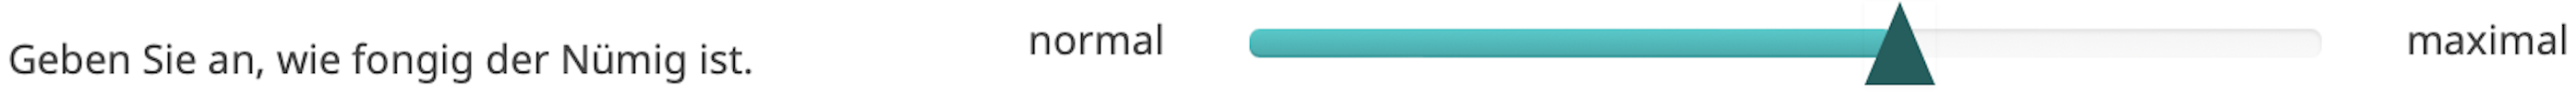
\includegraphics[width=\textwidth]{Aufg1_22}
  \caption[Darstellung der in Experiment 1 verwendeten Bewertungsskala zu Aufgabe I] {Darstellung der in Experiment 1 verwendeten Bewertungsskala zu Aufgabe I -- Skalarität.} 
  \label{Aufg1}
\end{figure}

%\noindent Die Skalenrange reichte von 0 bis 100 Punkte ohne dass die Werte eingeblendet wurden. Vom Anzeigen sowohl des Werts der Skalenendpunkte, von festgelegten Skalenmarken wie auch der gewählten Skalenposition wurde abgesehen, um unerwünschte Priming-Effekte zu umgehen. So wurde bspw. die Möglichkeit in Betracht gezogen, dass Binnendifferenzierungen wie Skalenmarken oder segmentale Abstufungen die Versuchspersonen dazu verleiten würden, alle Ausdrücke gleichermaßen um ebendiese Marke(n) herum anzuordnen, statt sich bei der Beurteilung gänzlich auf ihre persönliche Intuition zu verlassen.
\noindent Die zu Beginn farblose Skala war am linken Rand mit `normal' und am rechten Rand mit `maximal' beschriftet. Diese neutralen Bezeichnungen wurden aus der Intention heraus gewählt, numerische Skalenbeschriftungen (bspw. $0$ und $100$) oder dimensional gefärbte Ausdrücke wie \textit{Intensität} oder \textit{Stärke} zu vermeiden und unerwünschte Priming-Effekte zu verhindern. Dadurch sollten die Versuchspersonen so wenig wie möglich bei ihrer Wahrnehmung bzw. der Wahl der Reglerposition beeinflusst werden. Wurde der Schieberegler betätigt, so färbte sich der Bereich vom Nullpunkt bis zum ausgewählten Punkt hin farbig ein, mit dem Ziel den Versuchspersonen die zugeschriebene Intensität visuell zu verdeutlichen. Links neben der Bewertungsskala stand die Aufgabenstellung, die im Wortlaut dem jeweiligen Itemsatz angepasst war. Exemplarisch also: \textit{Geben Sie an, wie fongig der Nümig ist}.


Die zweite Aufgabe, die eine optisch beinahe identische Skala inkludierte, erfragte den im Satz ausgedrückten Grad an Sprechereinstellung. Diese Aufgabe befand sich auf der gleichen Webseite unmittelbar unter der ersten. Die Skala von {Aufgabe II} befindet sich in {Abbildung \ref{Aufg2}}.



%
\begin{figure}
  
\includegraphics[width=\textwidth]{Aufg2_22}
  \caption[Darstellung der in Experiment 1 verwendeten Bewertungsskala zu Aufgabe II] {Darstellung der in Experiment 1 verwendeten Bewertungsskala zu Aufgabe II -- Sprechereinstellung.} 
  \label{Aufg2}
\end{figure}

\noindent Die Skala zu Aufgabe II war zu Beginn ebenfalls farblos und entsprach der ersten in Gestalt und Betätigung. Auch hier war der Schieberegler intuitiv auf die zutreffende Skalenposition zu bewegen. Lediglich die Beschriftungen und die Aufgabenstellung unterschieden sich: Diese Skala war links mit `gar nicht' und rechts mit `maximal' gelabelt und erfragte den ausgedrückten Grad an Sprechereinstellung: \textit{Geben Sie an, wie stark der Sprecher seine persönliche Haltung zum beschriebenen Sachverhalt ausdrückt}. In der Aufgabenstellung wurde vom Gebrauch jeglicher Intensivierer (bspw. \textit{...\,, wie sehr der Sprecher\,...}) abgesehen und stattdessen auf das Adjektiv \textit{stark} zurückgegriffen.



%Die Skalenrange reichte jeweils von 0\,\% bis 100\,\%, ohne dass die Prozentwerte eingeblendet wurden. Vom Anzeigen sowohl des Werts der Skalenendpunkte wie auch der gewählten Skalenposition wurde abgesehen, um Priming-Effekte jeglicher Art zu umgehen. Die zu Beginn farblose Skala von Aufgabe I, die den Grad an Skalarität erfragte, war am linken Rand mit 'normal' und am rechten Rand mit 'maximal' beschriftet. Diese neutralen Bezeichnungen wurden aus der Intention heraus gewählt, dimensional gefärbte Ausdrücke wie \textit{Intensität} oder \textit{Stärke} zu vermeiden und die Versuchspersonen so wenig wie möglich bei ihrer Antwort bzw. der Wahl der Reglerposition zu beeinflussen. Wurde der Schieberegler betätigt, so färbte sich der Bereich vom Nullpunkt bis zum ausgewählten Punkt hin farbig ein, mit dem Ziel, den Versuchspersonen die zugeschriebene Intensität visuell zu verdeutlichen. Links neben der Skala befand sich die Aufgabenstellung, die im Wortlaut dem Itemsatz angepasst war: \textit{Geben Sie an, wie fongig der Nümig ist}. Zur Illustration ist die Skala von Aufgabe I in Abbildung 
%\ref{Aufg1} dargestellt.


%
%%
%\begin{figure}
%
%  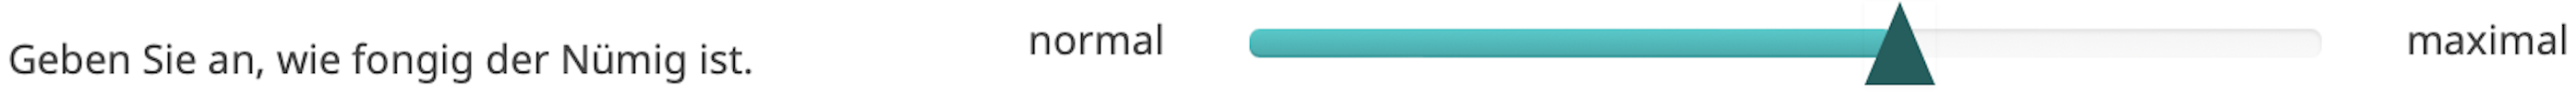
\includegraphics[width=1.005\textwidth]{Aufg1_22}
%  \caption[Darstellung der im Brückenexperiment verwendeten Bewertungsskala zu Aufgabe I] {Darstellung der im Brückenexperiment verwendeten Bewertungsskala zu Aufgabe I -- Skalarität.} 
%  \label{Aufg1}
%\end{figure}
%
%\noindent Die Skala von Aufgabe II, die auf den Grad an Sprechereinstellung abzielte, war zu Beginn ebenfalls farblos und entsprach der ersten in Gestalt und Betätigung. Lediglich die Beschriftungen und die Aufgabenstellung unterschieden sich: Diese Skala war links mit 'gar nicht' und rechts mit 'maximal' gelabelt und erfragte, wie stark der Sprecher seine persönliche Haltung zum beschriebenen Sachverhalt ausdrückt. In der Aufgabenstellung wurde vom Gebrauch jeglicher Intensivierer abgesehen und stattdessen auf das Adjektiv \textit{stark} zurückgegriffen.
%%Um vom Gebrauch jeglicher Intensivierer in der Aufgabenstellung abzusehen, wurde an der Stelle das Adjektiv \textit{stark} verwendet. 
%Die Skala von {Aufgabe II} befindet sich in {Abbildung \ref{Aufg2}}.



%%
%\begin{figure}
%
%  
\includegraphics[width=1.01\textwidth]{Aufg2_22}
%  \caption[Darstellung der in Experiment 1 verwendeten Bewertungsskala zu Aufgabe II] {Darstellung der in Experiment 1 verwendeten Bewertungsskala zu Aufgabe II -- Sprechereinstellung.} 
%  \label{Aufg2}
%\end{figure}

Die dritte Aufgabe war mithilfe einer komparativen Konstant-Summen-Skala zu erfüllen und erfragte die evaluative Einstellung des Sprechers zum bezeichneten Sachverhalt in Form von Abweichung von einer neutralen Mitte. Dabei wurden die Versuchspersonen dazu aufgefordert, mit einem festgelegten, virtuellen Geldbetrag zu wetten, ob die Satzaussage positiv, neutral oder negativ wertend zu verstehen ist bzw. ob der Sprecher dem Sachverhalt gegenüber positiv, neutral oder negativ eingestellt ist. Um die Aufgabe zu erledigen, sollten sie 100 Taler gemäß persönlicher Intuition restlos auf die zur Auswahl stehenden Felder `Positiv', `Neutral' und `Negativ' setzen. Diese Aufgabe wurde ebenso auf der gleichen Webseite direkt unter der zweiten angezeigt. Die im Experiment verwendete komparative Konstant-Summen-Skala zur Ermittlung der Einstellungspolarität ist mitsamt Aufgabenstellung in {Abbildung \ref{Aufg3} illustriert}.\footnote{Zu beachten ist, dass die Aufgabenstellung in der Abbildung aufgrund größtmöglicher Seitenskalierung verzerrt ist. Im Experiment umfasste diese zwei vollständig ausgefüllte Zeilen.}



%
\begin{figure}
  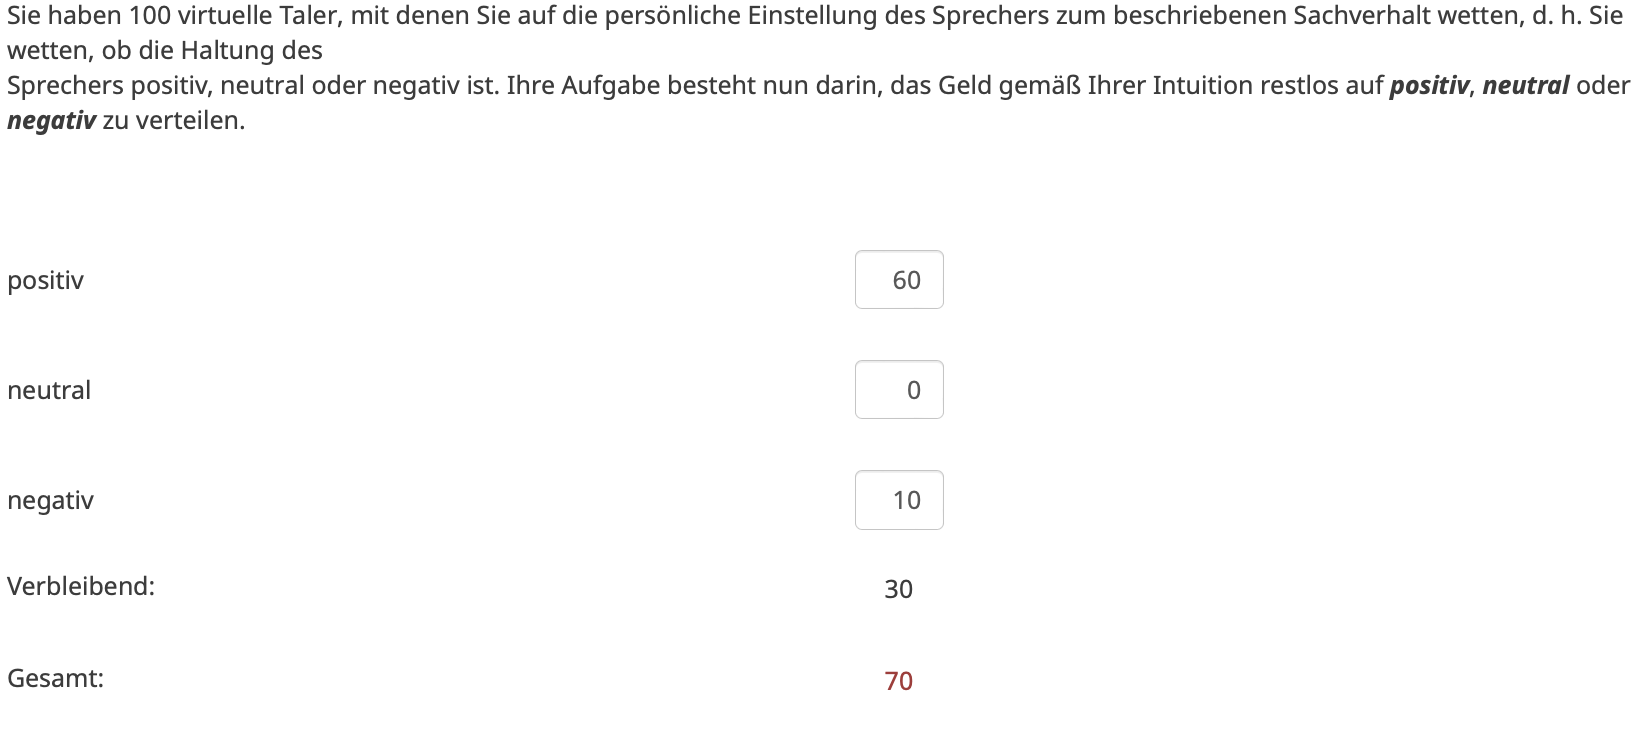
\includegraphics[width=\textwidth]{Aufg3_23}
  \caption[Darstellung der in Experiment 1 verwendeten Konstant-Summen-Skala zu Aufgabe III] {Darstellung der in Experiment 1 verwendeten Konstant-Summen-Skala zu Aufgabe III -- Einstellungspolarität.} 
  \label{Aufg3}
\end{figure}


\noindent Die noch einzusetzende Restmenge (`Verbleibend') sowie die Summe des bereits verteilten Geldes (`Gesamt') waren unter dem letzten Auswahlfeld eingeblendet. Die Taler mussten letztlich vollständig und in ganzen Zahlen auf die Felder aufgeteilt werden. Der Mehrwert einer komparativen Konstant-Summen-Skala liegt darin, dass die Versuchspersonen qua Abfragedesign dazu gezwungen sind, die Talersumme restlos aufzubrauchen und sie erst danach zur Beantwortung des nächsten Items übergehen können. Wie sie die Taler auf die Auswahlfelder verteilen, steht ihnen vollkommen frei. Durch dieses Vorgehen erhält man feinkörnige Abstufungen zwischen den Optionen.


Bevor das Experiment begann, wurden die Versuchspersonen in einer ausführlichen Instruktion samt beispielhafter Skalenabbildungen über den Anlass, die Dauer und den Ablauf des Experiments sowie datenschutzrechtliche Aspekte informiert. Außerdem wurden sie darum gebeten, das Experiment an einem Endgerät mit physischer Tastatur vorzunehmen, um zu verhindern, dass die Skalen aufgrund unterschiedlicher Bildschirmgröße (Smartphone/Tablet vs. Notebook/Desktop-PC) nicht korrekt angezeigt oder nicht wie vorgesehen bedient werden können.\footnote{Zur Kontrolle wurde im Experiment die Bildschirmgröße der {Versuchspersonen erfasst}.} Im Anschluss an die Einleitung folgten zunächst die Übungssätze, die gemäß dem Vorgehen bei den Testsätzen einzeln abgefragt wurden und nach der Beantwortung nahtlos und ohne weitere Erklärung in die für die Auswertung relevanten {Items übergingen}.


%Bei den abhängigen Variablen handelt es zum einen sich um die Skalenwerte, die die Versuchspersonen den Testsätzen zuschreiben sollten, sowie um die Taler, die sie auf die persönliche Einstellung des Sprechers wetten sollten. 



\section{Versuchspersonen}\label{abs:Versuchspersonen1}
Am Experiment haben insgesamt 71 deutsche Muttersprachler:innen im Alter von 18 bis 40 Jahren teilgenommen, die über die Crowdsourcing-Plattform \textit{Clickworker}\footnote{\citet[]{Rozsenich.2020}: \textit{https://www.clickworker.de} [letzter Aufruf: 23.06.2021].} rekrutiert und (bemessen an dem zu der Zeit gültigen deutschen Mindestlohn) mit je 1,70\,Euro entlohnt wurden. Über das Ziel der Untersuchung wurden die Versuchspersonen nicht informiert.


Wie die Vortests wurde die Untersuchung mittels \textit{LimeSurvey} erstellt und von den Versuchspersonen individuell online durchgeführt. Diesen wurde eine der 18 Listen zugeteilt. Die Dauer des Experiments betrug im Schnitt etwa zehn Minuten. Die Teilnahme erfolgte völlig anonym ohne Erhebung personenbezogener Angaben wie Alter, Geschlecht oder Herkunft, sodass keinerlei Rückschlüsse auf die Identität der Personen gezogen werden {konnten}.


Angestrebt wurde die Teilnahme von 72 Versuchspersonen, um zu gewährleisten, dass von jedem Intensivierer sowie der Nullvariante pro Liste vier Datenpunkte und somit eine gleichmäßige Verteilung vorliegt. Durch ein Problem von \textit{Clickworker} konnten nach Abschluss des Experiments jedoch nur Daten von 71 Personen exportiert werden. Aus diesem Grund standen für die Auswertung letztlich in Summe 17 Listen mit Daten von je vier Versuchspersonen sowie eine Liste mit Daten von drei Versuchspersonen zur Verfügung, was ein leichtes Ungleichgewicht nach sich zog. Da einzelne Personen von der Analyse ausgeschlossen werden mussten und die verwendeten linearen Regressionsmodelle als tolerant gelten, wurde angenommen, dass das bestehende Ungleichgewicht nicht relevant und vernachlässigbar ist. Zudem lässt sich bei Auswertungen häufig nicht vermeiden, dass einzelne Versuchspersonen unberücksichtigt bleiben, was ebenfalls zu Datenungleichgewichten führen kann.




\section{Ausschlusskriterien}
Im Vorfeld der Untersuchung wurden verschiedene Kriterien definiert, deren Zutreffen den Ausschluss einzelner Versuchspersonen zur Folge hatte. Ein Ausschluss von Personen kann dann erforderlich sein, wenn sich Anhaltspunkte für eine absichtliche Manipulation der Ergebnisse finden und der Einbezug ihrer Antworten gegebenenfalls zu verzerrten Resultaten führen würde. Zu den Ausschlusskriterien gehörten vorrangig eine überschnelle, schier unrealistische Reaktionszeit und ein uniformes Antwortmuster, die zusammen auf ein oberflächliches Durchführen des Experiments {schließen ließen}.


Von ursprünglich 71 Versuchspersonen wurden die Daten von vier Personen ausgeschlossen, weil sich bei ihnen der Verdacht erhärtete, dass sie das Experiment in Teilen oder auch als Ganzes nicht sorgfältig bearbeitet hatten. Dies resultierte in einem vollkommen einheitlichen Antwortmuster, das keinerlei Variation hinsichtlich der Skalenbewertung aufzeigte. So wurden z.\,B. alle Intensivierer inklusive der unmarkierten Variante gleichermaßen am linken oder rechten Skalenrand positioniert. Gestützt wurde diese Vermutung durch eine Begutachtung der durchschnittlichen Reaktionszeit je Item: Betrug diese bei allen Personen über die Dauer des Experiments hinweg im Schnitt 22,07 Sekunden (Standardabweichung (Englisch: \textit{standard deviation}, hier und im Folgenden abgekürzt mit \textit{SD} = 15,8), lag diese bei den ausgeklammerten Personen deutlich darunter (bspw. bei 5,94 Sekunden ({\textit{SD} = 1,8)} oder 6,59 Sekunden ({\textit{SD} = 1,0))}. Diese Schnelligkeit scheint angesichts der Menge der zu bewältigenden Aufgaben pro Item (zwei Mal Skaleneinschätzung und Aufteilung der Taler mittels Konstant-Summen-Skala) unrealistisch. Stattdessen ist davon auszugehen, dass diese knappe Zeitspanne in der Praxis kaum dazu ausreicht, um den zu bewertenden Satz sowie die Aufgabenstellungen zu lesen und zu verarbeiten; vor allem dann nicht, wenn unbekannte Pseudowörter darin enthalten sind und der durch den Satz ausgedrückte Grad auf eine Skala abgebildet werden soll. Um im Sinne der verfolgten Fragestellung repräsentative Ergebnisse zu erzielen, wurde der Ausschluss dieser Versuchspersonen als gerechtfertigt angesehen.





\section{Ergebnisse}\label{abs:Ergebnisse238}
%In diesem Abschnitt werden die Ergebnisse des Experiments vorgestellt. Dieses wurde zum einen mit dem Ziel durchgeführt, die Gültigkeit der noch ungeklärten Hypothesen H1-Temp und H1-Freq aus Kapitel \ref{Korpus} zu überprüfen, nach denen die Dauer oder Häufigkeit des Gebrauchs eines Intensivierers abträglich für dessen Expressivität ist (vgl. \citealt[59]{Tobler.1868}; {\citealt[2]{Hauschild.1899}}). Zum anderen wurde die Korrektheit der theoretischen Annahme getestet, dass Expressivität gleichermaßen mit einem höheren Grad an {Skalarität (vgl. H3)} und Sprechereinstellung (vgl. H4) einhergeht (vgl. {\citealt[315]{Lang.1983}}; {\citealt[22]{Paradis.1997}}; \citealt[57]{Ortner.2014}; {\citealt[133]{Gutzmann.2019a}}). Im Kontext letzterer wurde ferner die Polarität der Sprechereinstellung in die Untersuchung miteinbezogen, die bei expressiven Intensivierern aufgrund ihrer Einstellungsbezogenheit nach Auffassung von {\citet[135]{Gutzmann.2019a}} vielmehr positiv oder negativ als neutral interpretiert wird ({vgl. H5}).


Dieses Teilkapitel setzt sich aus deskriptiv- und inferenzstatistischer Datenanalyse zusammen und beginnt mit der Begutachtung der Ergebnisse von {Aufgabe I}, die die Skalarität ermittelte. Daraufhin werden die Daten von {Aufgabe II}, die auf die Sprechereinstellung abzielte, inspiziert. Vor diesem Hintergrund wird überprüft, ob expressive Intensivierer wirklich mit einem höheren Grad an Skalarität (vgl. H3) und Sprechereinstellung {(vgl. H4)} einhergehen, wie nach \citet[22]{Paradis.1997} und \citet[133]{Gutzmann.2019a} sowie {\citet[315]{Lang.1983}} und \citet[57]{Ortner.2014} anzunehmen ist. Da im Sinne von {\citet[133]{Gutzmann.2019a}} die Möglichkeit besteht, dass die Variablen \textsc{Skalarität} und \textsc{Sprechereinstellung} insofern korrelieren, als die Expressivität eines Intensivierers auf dessen Skalaritätsgrad einwirkt, wird im weiteren Verlauf ebendiesem möglichen Zusammenhang nachgegangen. Den Abschluss macht eine Betrachtung der Ergebnisse, die im Hinblick auf die in {Aufgabe III} abgefragte Einstellungspolarität erzielt wurden. In diesem Kontext wird untersucht, ob sich die Expressivität eines Intensivierers signifikant auf die Einschätzung der Einstellungspolarität auswirkt. So wird die Sprechereinstellung, die expressive Intensivierer ausdrücken, {\citet[135]{Gutzmann.2019a}} zufolge vielmehr positiv oder negativ als neutral interpretiert (vgl. H5).


Die statistischen Auswertungen wurden mithilfe von R ({Version 1.1.456}, \mbox{\citealt[]{R.2018}}) und den Paketen \textit{lme4} (\citealt[]{Bates.2015}) und \textit{lmerTest} ({\citealt[]{Kuznetsova.2017}}) vorgenommen. Die Visualisierung der Daten erfolgte außerdem mit \textit{ggplot2} ({\citealt[]{Wickham.2016}}). In der Untersuchung werden die drei klassischen Signifikanzniveaus `signifikant' ({\textit{p} < 0,05 $\star$}), `sehr signifikant' (\textit{p} < 0,01 $\star$$\star$) und `hochsignifikant' (\textit{p} < 0,001 $\star$$\star$$\star$) angenommen.\footnote{Der Asterisk (*) dient dazu, den jeweiligen \textit{p}-Wert gemäß dem zutreffenden Signifikanzniveau zu kennzeichnen.}
Bei der inferenzstatistischen Auswertung werden jeweils die im Zuge der Datenmodellierung berechneten linearen gemischten Regressionsmodelle vorgestellt. Um den einleitenden Fragen hinsichtlich dem Einfluss von Frequenz und Persistenz Rechnung zu tragen, wurden für die im Rahmen der Korpusuntersuchung eingeteilten Frequenz- und Persistenzgruppen ebenfalls Modelle berechnet, die jeweils im Anschluss an Aufgabe I und {Aufgabe II} präsentiert werden. Dadurch wird getestet, ob eine hohe Frequenz (vgl. H1-Freq) oder ein persistenter Gebrauch (vgl. H1-Temp) tatsächlich abträglich für die Expressivität eines Intensivierers ist, wie \citet[2]{Hauschild.1899} und {\citet[59]{Tobler.1868}} postulieren. Weil letztere Berechnungen lediglich die Gruppe der expressiven Intensivierer betreffen, wurden die deskriptive und unmarkierte Stufe bei diesen Regressionsanalysen außen vor gelassen. Die für die beiden Faktoren Frequenz und Persistenz berechneten Modelle schließen sich jeweils an die Modelle zu Aufgabe I und Aufgabe II an. An dieser Stelle sei erwähnt, dass die Faktoren nicht unabhängig voneinander, sondern inhärent zusammenhängend sind. Dabei wird lediglich der Faktor Frequenz variiert, während der Faktor Persistenz in dem Sinne konstant bleibt, dass die drei neuen Intensivierer grundsätzlich mit einer niedrigen Frequenz auftreten.








\subsection{Aufgabe I -- Skalarität} \label{abs:VP-Vergleich1251}


\subsubsection{Vergleich der Stufen} \label{abs:I-Vergleich254}


In Tabelle \ref{SkaWe1} sind die gemittelten Skalenwerte, d.\,h. das arithmetische Mittel, sowie die Standardabweichungen, basierend auf 67 Datenpunkten pro Intensivierer bzw. der unintensivierten Variante, zu Aufgabe I aufgeführt. Die 16 expressiven Intensivierer werden zunächst zu einer Stufe zusammengefasst und mit den beiden Kontrollstufen kontrastiert. Die Tabelle bildet daher die Werte von drei Stufen (d.\,h. deskriptiv, expressiv und unmarkiert)  in alphabetischer Reihenfolge ab.

%
\begin{table}
%\setlength{\tabcolsep}{16pt}
\begin{tabularx}{.8\textwidth}{lYY}
\lsptoprule
%            & \textbf{Aufgabe I}  & \\
%            & \textbf{Skalarität} & \\
Stufe      & Skalenwert     &\textit{SD}\\
\midrule
deskriptiv & 63,90          & 17,9\\
expressiv  & 67,70          & 22,4\\
unmarkiert & 35,27          & 27,4\\
\lspbottomrule
\end{tabularx}
\caption[Gemittelte Skalenwerte der Stufen bei {Aufgabe I} von Experiment 1]{Gemittelte Skalenwerte und Standardabweichungen der Stufen bei Aufgabe I -- Skalarität (in alphabetischer Reihenfolge).}
\label{SkaWe1}
\end{table}


\noindent Die Werte aus Tabelle \ref{SkaWe1} weisen darauf hin, dass die expressiven Intensivierer nach Einschätzung der Versuchspersonen insgesamt eine höhere Skalenposition einnehmen als der deskriptive Intensivierer oder die unmarkierte Variante. So wurde die expressive Stufe diesbezüglich mit 67,70 Punkten auf der Skala am höchsten verortet, wohingegen der deskriptiven Stufe von den Versuchspersonen ein um etwa 3,80 Punkte niedrigerer Skalenwert zugewiesen wurde. Weit abgeschlagen dahinter befindet sich die unmarkierte Stufe, deren Wert sich von der expressiven Stufe um ca. 32,43 Punkte, von der deskriptiven Stufe um {ca. 28,63 Punkte} unterscheidet. Dies deutet erwartungsgemäß auf eine in der Skalarität abnehmende Rangfolge der {Stufen hin}.


Dieses Ergebnis ist in Abbildung \ref{SkalarBox} mittels Boxplots, auch Kastengrafik genannt, dargestellt. Die von der Box nach oben und unten reichenden Whiskers verdeutlichen die Varianz der Skalenbewertung und geben an, wie stark das Skalenspektrum von den Versuchspersonen genutzt wurde. Die Querstriche oben und unten symbolisieren das Maximum und Minimum der Whiskers und somit die Extremwerte, die noch keine Ausreißer sind, während die Einkerbung innerhalb der Box für den Median steht. Die beiden Quartile, aus denen die Box besteht, geben die Verteilung der Skalenwerte um den Median herum an. Darüber hinaus stellen die Kreise Ausreißer dar, deren Abstand mehr als anderthalb Interquartile von der Box entfernt liegen (vgl. \citealt[77f.]{Mittag.2016};; \citealt[579]{Wollschlaeger.2017}).


%
\begin{figure}
  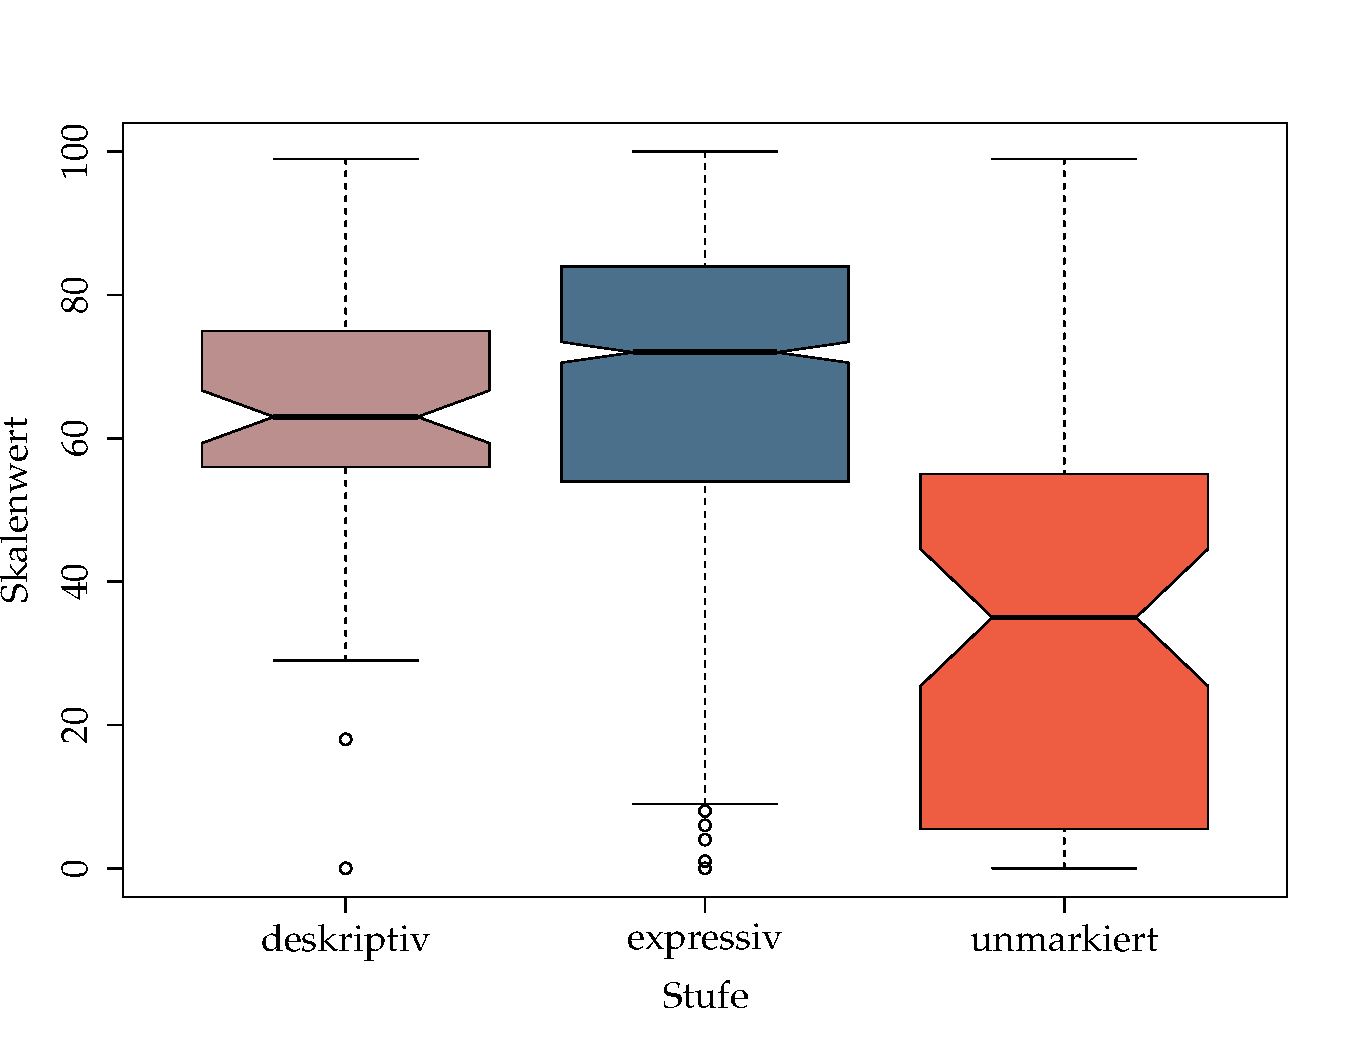
\includegraphics[width=1\textwidth]{BoxSkalar_1}
	\caption[Gemittelte Skalenwerte der Stufen bei {Aufgabe I} von Experiment 1]{Gemittelte Skalenwerte der Stufen bei Aufgabe I -- Skalarität ({x-Achse =} Stufe, y-Achse = Skalenwert).}
  \label{SkalarBox}
\end{figure}


%
\subsubsection{Regressionsanalysen zum Vergleich der Stufen}


Mit dem Ziel die soeben beschriebenen deskriptivstatistischen Ergebnisse auf ihre Signifikanz hin zu überprüfen, wurden sie einer zusätzlichen inferenzstatistischen Auswertung unterzogen. Wie eingangs beschrieben, wurden die Daten mittels R und den Paketen \textit{lme4} (\citealt[]{Bates.2015}) und \textit{lmerTest} ({\citealt[]{Kuznetsova.2017}}) ausgewertet. Hierzu wurden lineare gemischte Modelle berechnet, die aus der unabhängigen Variable die abhängige Variable voraussagen. Im Rahmen der Regressionsanalyse für Aufgabe I wurde zunächst ein volles Modell mit den Effekten aller unabhängigen Variablen und deren Zwei-Wege-Interaktionen berechnet, die eventuell einen Einfluss auf die abhängige Variable hatten. Das volle Modell beinhaltete \textit{Fixed Effects} für den \textsc{Skalenwert}, die \textsc{Stufe}, die \textsc{Position}\footnote{\textit{Position} meint hier und im weiteren Verlauf die Position eines Items im Experiment.} sowie deren Zwei-Wege-Interaktionen. Der \textsc{Skalenwert} wurde dabei als metrische abhängige Variable modelliert, die \textsc{Stufe} und die \textsc{Position} als kategoriale Prädiktoren. Die Variable \textsc{Skalenwert} steht bei dieser Aufgabe für den Skalaritätsgrad, den die Versuchspersonen mit der jeweiligen Stufe oder dem jeweiligen Intensivierer verbunden haben. Um einen möglichen graduellen Effekt und Unterschiede zwischen den drei Stufen zu finden, wurde das Referenzlevel `Expressiv' jeweils mit `Deskriptiv' und `Unmarkiert' verglichen. Dazu wurden die Ausprägungsformen der mehrkategorialen Variable \textsc{Stufe} (d.\,h. deskriptiv, expressiv und unmarkiert) per Dummy-Codierung in zwei Schritten (d.\,h. `Expressiv' vs. `Deskriptiv' und `Expressiv' vs. `Unmarkiert') als $0$ und $1$ kodiert und somit nach binären Kontrasten gesplittet {\citep[vgl.][407, 442]{Sauer.2019}}. Dadurch wurden aus einer unabhängigen Variable mit drei Stufen zwei unabhängige Variablen mit je zwei Stufen. Zudem wurden im Modell versuchspersonen- und itemweise \textit{Random Intercepts} und \textit{Random Slopes} für die Variablen \textsc{Skalenwert}, \textsc{Stufe} und \textsc{Position} miteinbezogen.  Das bedeutet, dass im Modell ebenso potenzielle Unterschiede zwischen den Versuchspersonen und Pseudowörtern berücksichtigt wurden. Ausgehend vom vollen Regressionsmodell wurden durch das Prinzip der \textit{Backward Model Selection}, auch Rückwärtsselektion genannt, schrittweise alle Effekte getilgt, die den Modell-Fit nicht signifikant verbesserten. Begonnen wurde jeweils mit dem Effekt, der nach der Berechnung mit {\textit{lmerTest} (\citealt[]{Kuznetsova.2017})} den höchsten \textit{p}-Wert aufwies. Dieser wurde im nächsten Schritt beim neuen Modell entfernt und das Modell so sukzessive vereinfacht. Daraufhin wurden die beiden Modelle mithilfe von Likelihood-Quotienten-Tests bzw. Chi$^{2}$-Tests mit der Funktion \textit{anova} in R kontrastiert: Wenn das komplexere Modell die Daten nicht signifikant besser erklärte, wurde das einfachere Modell bevorzugt. Auf diese Weise konnte das optimale Regressionsmodell gefunden werden.


Nachdem durch dieses Vorgehen mehrere Modelle mittels Rückwärtsselektion und der \textit{anova}-Funktion in Bezug auf die statistische Signifikanz des Unterschiedes miteinander verglichen wurden, konnte ein finales Modell mit ausschließlich signifikanten Effekten abgeleitet werden. Dieses gibt den Einfluss der unabhängigen Variablen auf die abhängige Variable an. In der Tabelle, die das jeweilige finale Regressionsmodell abbildet, ist neben dem \textit{$\chi$$^{2}$}-Wert und \textit{p}-Wert der Standardfehler (englisch: \textit{standard error}, hier und im Folgenden abgekürzt mit \textit{SE}) angegeben, der die Streuung der Daten wiedergibt {\citep[vgl.][273]{Sauer.2019}}. Zudem ist der Regressionskoeffizient {(= \textit{Estimate}}) gelistet, der den \glqq{}Einfluss des Prädiktors\grqq{} ({\citealt[351]{Sauer.2019}}) {anzeige}. Die vollen und finalen Regressionsmodelle zu diesem Experiment sind im {Anhang \ref{Regr1}} separiert nach Aufgabe I (Skalarität), Aufgabe II (Sprechereinstellung) und {Aufgabe III} (Einstellungspolarität) gesammelt.


Das finale Modell enthält signifikante Haupteffekte für die Prädiktoren \textsc{Stufe} und \textsc{Position}. Diese Koeffizienten sind in {Tabelle \ref{LinReg0001}} zu finden.


%
\begin{table}
%\setlength{\tabcolsep}{9.375pt}
\begin{tabularx}{\textwidth}{Xccccr}
\lsptoprule
Prädiktor & \textit{Est.} & \textit{SE} & \textit{$\chi$$^{2}$} & \textit{p} & \\
\midrule
(Intercept) & \textcolor{white}{-}67,88 & 1,98 & 124,15 & < 0,001 & $\star$$\star$$\star$\\
Expressiv vs. Unmarkiert & -32,56 & 3,39 & \textcolor{white}{-}54,42 & < 0,001 & $\star$$\star$$\star$\\
Expressiv vs. Deskriptiv & \textcolor{white}{-}\textcolor{white}{-}-5,11 & 2,56 & \textcolor{white}{-}\textcolor{white}{-}3,74 & < 0,05 & $\star$ \\
Position & \textcolor{white}{-}\textcolor{white}{-}-1,70 & 0,63 & \textcolor{white}{-}\textcolor{white}{-}6,90 & < 0,01 & \multicolumn{1}{r}{$\star$$\star$} \\
\lspbottomrule
\end{tabularx}
\caption[Finales Regressionsmodell zu Aufgabe I von Experiment 1 (mit `Expressiv' als Referenzlevel)]{Finales Regressionsmodell zu Aufgabe I -- Skalarität (mit `Expressiv' als Referenzlevel).}
\label{LinReg0001}
\end{table}

\noindent Dem in Tabelle \ref{LinReg0001} dargelegten Modell nach haben zwei unabhängige Variablen einen hohen Einfluss auf die abhängige Variable, d.\,h. den Skalenwert: \textsc{Stufe} und \textsc{Position}. Zum einen ist der festgestellte Unterschied zwischen der expressiven und der unmarkierten Stufe signifikant {($\chi$$^{2}$\,(1) = 54,42}, {\textit{p} < 0,001}), sprich Sätzen mit expressivem Intensivierer wird im Allgemeinen eine signifikant höhere Skalenposition zugeschrieben als unintensivierten Sätzen. Zum anderen ist ein signifikanter Unterschied zwischen der expressiven und der deskriptiven Stufe auszumachen {($\chi$$^{2}$\,(1) = 3,74}, \textit{p} < 0,05). Somit werden neben unintensivierten Sätzen auch Sätze mit deskriptivem Intensivierer auf der Skala signifikant niedriger gerankt als Sätze mit expressivem Intensivierer. Daneben zeigt sich ein signifikanter Positionseffekt ({$\chi$$^{2}$\,(1) = 6,90}, {\textit{p} < 0,01}), der wie folgt zu interpretieren ist: Je später ein Item im Experiment auftritt, desto niedriger ist seine Bewertung auf der Skala. Dies deutet auf einen strategischen Gewöhnungseffekt hin, in dessen Folge der zu Beginn als stärker wahrgenommene Unterschied zwischen den Stufen im Laufe des Experiments nach und nach kleiner geworden ist.


In einer weiteren Analyse wurde das Referenzlevel der mehrkategorialen Variable \textsc{Stufe} auf `Unmarkiert' gesetzt, was bedeutet, dass `Unmarkiert' jeweils mit `Expressiv' und `Deskriptiv' kontrastiert wurde. Vor diesem Hintergrund drängt sich die Frage auf, ob die Kontrollstufe, d.\,h. die unmarkierten Sätze, prinzipiell mit einem signifikant niedrigeren Skalaritätsgrad assoziiert werden und sich dahingehend sowohl von der expressiven als auch der deskriptiven Stufe unterscheiden. Das methodische Vorgehen entsprach dem obigen: Wie zuvor wurde zunächst ein volles Regressionsmodell berechnet, in dem nach Rückwärtsselektion und Modellvergleich sukzessive all diejenigen Effekte weggelassen wurden, die sich nicht signifikant auf die abhängige Variable ausgewirkt haben. Die \textit{Random-Effects}-Struktur wurde mit Ausnahme des Referenzlevels der beiden binären Vergleiche nicht verändert. Das finale Modell beinhaltet signifikante Haupteffekte für die Prädiktoren \textsc{Stufe} und \textsc{Position}. Die berechneten Koeffizienten sind in {Tabelle \ref{LinReg0010}} {aufgeführt}.

%
\begin{table}
\begin{tabularx}{\textwidth}{Xccccr}
\lsptoprule
Prädiktor & \textit{Est.} & \textit{SE} & \textit{$\chi$$^{2}$} & \textit{p} & \\
\midrule
(Intercept) & 35,33 & 3,18 & 70,60 & < 0,001 & $\star$$\star$$\star$\\
Unmarkiert vs. Expressiv & 32,55 & 3,39 & 54,35 & < 0,001 & $\star$$\star$$\star$\\
Unmarkiert vs. Deskriptiv & 27,43 & 3,33 & 44,02 & < 0,001 & $\star$$\star$$\star$\\
Position & \textcolor{white}{-}-1,71 & 0,63 & \textcolor{white}{-}6,96 & < 0,01 & \multicolumn{1}{r}{$\star$$\star$} \\
\lspbottomrule
\end{tabularx}
\caption[Finales Regressionsmodell zu Aufgabe I von Experiment 1 (mit `Unmarkiert' als Referenzlevel)]{Finales Regressionsmodell zu Aufgabe I -- Skalarität (mit `Unmarkiert' als Referenzlevel).}
\label{LinReg0010}
\end{table}


\noindent Die in Tabelle \ref{LinReg0010} zusammengetragenen Werte erhärten die zu testende Annahme: Die unmarkierte Stufe unterscheidet sich nicht nur signifikant von der expressiven Stufe ($\chi$$^{2}$\,(1) = 54,35, \textit{p} < 0,001), sondern auch von der deskriptiven Stufe ({$\chi$$^{2}$\,(1) = 44,02}, \textit{p} < 0,001). Dies zeigt, dass die Methode mit unintensivierten Sätzen als Kontrollstufe in dem Sinne funktioniert hat, dass sie im Vergleich zu mittels deskriptivem oder expressivem Intensivierer modifizierten Sätze von den Versuchspersonen auf der Skala grundsätzlich niedriger positioniert wurden. Darüber hinaus findet sich ein signifikanter Positionseffekt {($\chi$$^{2}$\,(1) = 6,96}, {\textit{p} < 0,01)}: Je fortgeschrittener die Position eines Items im Experiment ist, desto niedriger wird der Grad an Skalarität evaluiert.


Kurz gefasst belegen die Ergebnisse von Aufgabe I den in der Literatur angenommenen Unterschied zwischen der deskriptiven und expressiven Intensiviererklasse (vgl. \citealt[22]{Paradis.1997}; {\citealt[133]{Gutzmann.2019a}}). So wurde der Skalaritätsgrad von Sätzen mit expressivem Intensivierer von den Versuchspersonen in der Tat als signifikant höher empfunden als der von Sätzen, die im Experiment mit dem deskriptiven oder ohne Intensivierer präsentiert wurden. Dass sich der Unterschied zwischen den drei Stufen derart deutlich zeigt, lässt außerdem den Schluss zu, dass das Skalenrating als Untersuchungsmethode funktioniert hat.


\subsubsection{Vergleich der Intensivierer} \label{abs:I-Vergleich339}


In Tabelle \ref{SkaWe2} werden der gemittelte Skalenwert und die Standardabweichung für die einzelnen Intensivierer bei Aufgabe I dargelegt. Dies bietet einen detaillierten Überblick über die Einschätzung der Versuchspersonen und ermöglicht, die im Experiment abgefragten Ausdrücke in Bezug auf den ihnen zugeschriebenen Skalaritätsgrad miteinander zu vergleichen. Die expressiven Intensivierer sind in ansteigendem Skalenwert angeordnet.


%Diese Werte sind inklusive Standardabweichungen in Tabelle \ref{SkaWe2} aufgeführt.





\begin{table}
%\setlength{\tabcolsep}{32.75pt}
\begin{tabularx}{.8\textwidth}{llYY}
\lsptoprule
%       &  \multicolumn{1}{c}{\textbf{Aufgabe I}} &  \\
%       &  \multicolumn{1}{c}{\textbf{Skalarität}} &  \\  [0.5em]
Stufe & Intensivierer & Skalenwert &\textit{SD}\\
\midrule
\rowcolor[gray]{.90}
deskriptiv & \textit{sehr} &  63,90 & 17,9\\
expressiv  & \textit{arg}  &  59,87 & 20,8\\
\rowcolor[gray]{.90}
           & \textit{voll} &  62,40 & 22,4\\
           & \textit{ober} &  62,84 & 22,9\\
\rowcolor[gray]{.90}
           & \textit{derb} &  63,36 & 20,3\\
           & \textit{sau}  &  65,14 & 22,7\\
\rowcolor[gray]{.90}
           & \textit{unheimlich} &  65,78 & 24,1\\
           & \textit{verdammt}   &  67,05 & 20,5\\
\rowcolor[gray]{.90}
           & \textit{fürchterlich} &  68,05 & 23,0\\
           & \textit{furchtbar}    &  68,99 & 22,4\\
\rowcolor[gray]{.90}
           & \textit{krass}       &  69,02 & 22,4\\
           & \textit{schrecklich} &  70,09 & 20,0\\
\rowcolor[gray]{.90}
           & \textit{hammer} &  70,70 & 22,9\\
           & \textit{scheiß} &  71,36 & 25,0\\
\rowcolor[gray]{.90}
           & \textit{wahnsinnig} &  71,37 & 23,2\\
           & \textit{super}      &  72,51 & 19,0\\
\rowcolor[gray]{.90}
           & \textit{mega}        &  74,66 & 22,4\\
\multicolumn{1}{l}{unmarkiert} & \textit{$\emptyset$} &  35,27 & 27,4\\
\lspbottomrule
\end{tabularx}
\caption[Gemittelte Skalenwerte der einzelnen Intensivierer bei Aufgabe I von Experiment 1]{Gemittelte Skalenwerte und Standardabweichungen der einzelnen Intensivierer bei Aufgabe I -- Skalarität (angeordnet nach ansteigendem Skalenwert der expressiven Intensivierer).}
\label{SkaWe2}
\end{table}


%
\noindent Der Übersicht in Tabelle \ref{SkaWe2} ist zu entnehmen, dass sich der deskriptive Intensivierer \textit{sehr} bei Aufgabe I kaum von den expressiven Intensivierern unterscheidet. So liegt der gemittelte Skalenwert von \textit{sehr} mit 63,90 Punkten partiell sogar über dem Wert mancher expressiver Intensivierer: {\textit{arg} (59,87 Punkte)}, {\textit{voll} (62,40 Punkte)}, {\textit{ober} (62,84 Punkte)} und \textit{derb} (63,36 Punkte). Wie im Hinblick auf {Tabelle \ref{SkaWe1}} beschrieben, wurde die unmarkierte Variante mit durchschnittlich 35,27 Punkten niedrig bewertet. Schaut man sich das Skalenspektrum der expressiven Intensivierer an, ist festzustellen, dass sich deren Werte alle in einem mittleren Skalenbereich von {59,87 Punkten (\textit{arg})} und 74,66 Punkten (\textit{mega}) bewegen. Somit beträgt die Differenz zwischen dem am niedrigsten und dem am höchsten eingestuften expressiven Intensivierer etwa 14,79 Punkte. Diese Tendenzen sind im {Anhang \ref{Rat1}} in {Abbildung \ref{Skalar7}} mittels Säulendiagramm grafisch dargestellt. Zudem findet sich im {Anhang \ref{Pseu1}} in {Tabelle \ref{Pseudos1}} eine Übersicht der gemittelten Skalenwerte jeder Kombination aus Pseudonomen und Pseudoadjektiv. Darin ist zu erkennen, dass die Pseudowörter über ähnliche Werte verfügen. So weist die Kombination aus \textit{Das Gedalst} und \textit{wübig} mit durchschnittlich 62,55 Punkten den niedrigsten Skalenwert auf, wohingegen die Kombination aus \textit{Das Zafche} und \textit{göcktig} mit 69,69 Punkten auf der Skala am höchsten beurteilt wurde ($\Delta$ = ca. 7,14 Punkte).\footnote{Das Symbol Delta ($\Delta$) steht hier und im Folgenden für die Differenz zwischen zwei Werten.} Zur besseren Anschaulichkeit sind die gemittelten Skalenwerte je Kombination aus Pseudonomen und Pseudoadjektiv im Anhang \ref{Happy0} in {Abbildung \ref{Happy3}} mithilfe eines Säulendiagramms visualisiert. Die nur geringe Differenz zwischen den einzelnen Pseudowort-Kombinationen deutet darauf hin, dass die Verwendung von Pseudowörtern einen Einfluss der semantischen Eigenschaften verhindert und die Untersuchungsmethode funktioniert hat. Wäre der Unterschied zwischen ihnen an dieser Stelle ausgeprägter, so ließe sich spekulieren, dass die zugeschriebenen Skalenwerte durch die Pseudowörter beeinflusst gewesen sein könnten. Dies scheint jedoch nicht der Fall zu sein.


\subsubsection{Regressionsanalyse zu Frequenz und Persistenz}


Im Folgenden wird dem möglichen Einfluss von Frequenz (vgl. H1-Freq) und Persistenz (vgl. H1-Temp) auf den Skalaritätsgrad nachgegangen. Diese Überprüfung richtet sich nach der Gruppeneinteilung (d.\,h. `Hochfrequent' vs. `Niedrigfrequent' für H1-Freq sowie `Alt' vs. `Neu' für {H1-Temp}), die sich auf Grundlage der Untersuchungsergebnisse der in Kapitel \ref{Korpus} präsentierten Korpusstudie vornehmen ließ. Da die Korpusdaten klar für die Annahme zweier unterschiedlicher Frequenz- und Persistenzgruppen sprachen, wurde bei diesen Regressionsanalysen mit kategorialen statt kontinuierlichen Variablen gerechnet.


Zunächst wird die Hypothese H1-Freq beschrieben. Nach dieser sind oft vorkommende Intensivierer weniger expressiv als seltene Intensivierer \citep[vgl.][2]{Hauschild.1899}. Die Häufigkeiten konnten im Rahmen der in Kapitel \ref{Korpus} vorgestellten Korpusstudie abgeleitet werden. Auf Basis der Korpusfrequenz des letzten Zeitabschnitts (d.\,h. dem Zeitraum von 1990 bis 2017) wurden die expressiven Intensivierer in eine niedrigfrequente (n = 9) und eine hochfrequente {(n = 7)} Gruppe eingeordnet (vgl. Tabelle \ref{Fre3.1}). Diese Gruppen wurden im vollen Regressionsmodell als Ausgangspunkt gewählt, um den potenziellen Einfluss von Frequenz und somit die Gültigkeit von H1-Freq zu überprüfen.


Im Hinblick auf H1-Temp wurden in Abhängigkeit des Erstvorkommens ebenfalls zwei Gruppen gebildet. Dies geschah vor dem Hintergrund der Einschätzung, dass lange gebrauchte Intensivierer weniger expressiv sind als neuere Intensivierer \citep[vgl.][59]{Tobler.1868}. Anhand der in der Korpusstudie abgeleiteten diachronen Entwicklungsverläufe konnten drei Intensivierer detektiert werden, die erst im Laufe des Untersuchungszeitraums im Korpus in Erscheinung getreten sind, nämlich \textit{hammer}, \textit{krass} und \textit{mega}. Diese wurden bei der Datenmodellierung von den restlichen Ausdrücken (n = 13) separiert und im vollen Modell als Gruppe der neuen Intensivierer berücksichtigt.


Wiederholt kam das oben beschriebene statistische Vorgehen zum Einsatz. Zunächst wurde ein volles Regressionsmodell berechnet, in dem mithilfe von Rückwärtsselektion und \textit{anova}-Modellvergleich sukzessive alle Effekte ausgeschlossen wurden, die den Modell-Fit nicht signifikant verbesserten. Das volle Modell enthielt \textit{Fixed Effects} für die kategorialen Prädiktoren \textsc{Frequenzgruppe}, \textsc{Persistenzgruppe}, \textsc{Position} sowie deren Zwei-Wege-Interaktionen. Der \textsc{Skalenwert} wurde erneut als metrische abhängige Variable modelliert; er steht in diesem Fall für den Skalaritätsgrad, den die Versuchspersonen der jeweiligen Stufe oder dem jeweiligen Intensivierer zugesprochen haben. Um mögliche Unterschiede zwischen hoch- und niedrigfrequenten Ausdrücken zu finden, wurde die binäre nominale Variable \textsc{Frequenzgruppe} dummy-gecoded. Dabei wurde der Stufe `Hoch' der {Wert $0$} und der Stufe `Niedrig' der {Wert $1$} zugewiesen. Daneben wurde auch die binäre nominale Variable \textsc{Persistenzgruppe} dummy-gecoded, wobei die Stufe `Alt' als $0$ und die Stufe `Neu' als $1$ codiert wurde. Diese Stufen wurden anschließend jeweils miteinander verglichen. Außerdem wurden im vollen Modell versuchspersonen- und itemweise \textit{Random Intercepts} und \textit{Random Slopes} für die Variablen \textsc{Skalenwert}, \textsc{Frequenzgruppe}, \textsc{Persistenzgruppe} und \textsc{Position} miteingerechnet, sodass auch potenzielle Unterschiede zwischen den Versuchspersonen und Pseudowörtern berücksichtigt wurden. Das finale Modell beinhaltet signifikante Haupteffekte für die Prädiktoren \textsc{Frequenzgruppe}, \textsc{Persistenzgruppe} und \textsc{Position}. Die berechneten Koeffizienten sind in {Tabelle \ref{LinRea0100}}.

 %
\begin{table}
%\setlength{\tabcolsep}{13.55pt}
\begin{tabularx}{.8\textwidth}{Xrrrrr}
\lsptoprule
Prädiktor & \textit{Est.} & \textit{SE} & \textit{$\chi$$^{2}$} & \textit{p} & \\
\midrule
(Intercept) & 70,96 & 2,29 & 30,94 & < 0,001 & $\star$$\star$$\star$\\
Alt vs. Neu & \textcolor{white}{-}5,91 & 1,36 & 16,58 & < 0,001 & $\star$$\star$$\star$\\
Hoch vs. Niedrig & -2,49 & 1,06 & \textcolor{white}{-}5,31 & < 0,05 & $\star$\\
Position & -0,31 & 0,13 & \textcolor{white}{-}5,95 & < 0,05 & $\star$\\
\lspbottomrule
\end{tabularx}
\caption[Finales Regressionsmodell zu Aufgabe I von Experiment 1 (Frequenz mit `Hoch' als Referenzlevel, Persistenz mit `Alt' als Referenzlevel)]{Finales Regressionsmodell zu Aufgabe I -- Skalarität (Frequenz mit `Hoch' als Referenzlevel, Persistenz mit `Alt' als Referenzlevel).}
\label{LinRea0100}
\end{table}

\noindent Das in Tabelle \ref{LinRea0100} dargelegte Regressionsmodell zeigt in Bezug auf Skalarität zum einen einen statistisch signifikanten Unterschied zwischen den beiden Persistenzgruppen an {($\chi$$^{2}$\,(1) = 16,58}, \textit{p} < 0,001). Demnach wird der Grad an Skalarität bei neuen Intensivierern auf der Skala insgesamt höher bewertet als bei älteren Intensivierern. Mit anderen Worten: Der eingeschätzte Skalaritätsgrad der neuen Intensivierer \textit{hammer}, \textit{krass} und \textit{mega} unterscheidet sich signifikant von dem der restlichen Intensivierer. Zum anderen unterscheiden sich auch die beiden Frequenzgruppen signifikant voneinander {($\chi$$^{2}$\,(1) = 5,31}, {\textit{p} < 0,05)}. Das bedeutet, dass die Versuchspersonen Sätze mit niedrigfrequenten Intensivierern mit einem niedrigeren Grad an Skalarität assoziiert haben als Sätze, die im Experiment mit hochfrequenten Intensivierern präsentiert wurden. Weiterhin ist ein signifikanter Positionseffekt auszumachen ({$\chi$$^{2}$\,(1) = 5,95}, \textit{p} < 0,05), der darauf hinweist, dass die eingeschätzte Skalarität mit fortschreitendem Experiment abnimmt. Dieser Befund legt einen Gewöhnungseffekt nahe, der sich bei den Versuchspersonen über die Dauer des Experiments hinweg eingestellt zu haben scheint.


Von den Ergebnissen der Regressionsanalyse ausgehend lässt sich zusammenfassen, dass die beiden Faktoren Frequenz und Persistenz anscheinend durchaus einen signifikanten Effekt auf die wahrgenommene Skalarität haben. So verbanden die Versuchspersonen die im Korpus rezent etablierten Intensivierer \textit{hammer}, \textit{krass} und \textit{mega} grundsätzlich mit einem höheren Skalaritätsgrad als die älteren Intensivierer. Darüber hinaus wird auch der Grad an Skalarität bei den hochfrequenten Intensivierern in Summe als deutlich stärker empfunden als bei den niedrigfrequenten Intensivierern. Dies lässt den Schluss zu, dass der Skalaritätsgrad mit zunehmender Frequenz ansteigt.




\subsection{Aufgabe II -- Sprechereinstellung} \label{abs:VP-Vergleich2423}


\subsubsection{Vergleich der Stufen} \label{abs:I-Vergleich426}


Tabelle \ref{SkaWex} bietet einen Überblick über die gemittelten Skalenwerte und Standardabweichungen für die  Stufen zu Aufgabe II. Wie zuvor sind die expressiven Intensivierer zunächst zu einer Stufe zusammengefasst.


\begin{table}
%\setlength{\tabcolsep}{16pt}
\begin{tabularx}{.8\textwidth}{lYY}
\lsptoprule
%   & \textbf{Aufgabe II} & \\
%  & \textbf{Sprechereinstellung} &\\
Stufe & Skalenwert &\textit{SD}\\
\midrule
deskriptiv & 42,34 & 23,3\\
expressiv  & 65,24 & 24,9\\
unmarkiert & 30,11 & 26,2\\
\lspbottomrule
\end{tabularx}
\caption[Gemittelte Skalenwerte der Stufen bei {Aufgabe II} von Experiment 1]{Gemittelte Skalenwerte und Standardabweichungen der Stufen bei Aufgabe II -- Sprechereinstellung (in alphabetischer Reihenfolge).}
\label{SkaWex}
\end{table}


\noindent Den Werten aus Tabelle \ref{SkaWex} nach wurden Sätze mit expressivem Intensivierer von den Versuchspersonen auf der Skala erheblich höher gerankt als Sätze mit deskriptivem Intensivierer oder die unmarkierte Variante. So wurden der expressiven Stufe im Schnitt {65,24 Punkte} zugeschrieben, wohingegen die deskriptive Stufe auf der Skala durchschnittlich bei 42,34 Punkten und somit um etwa 22,90 Punkte niedriger positioniert wurde. Schlusslicht hinsichtlich Sprechereinstellung bildet erwartungsgemäß die unmarkierte Variante, die eine Differenz von ca. 35,13 Punkten zur expressiven Stufe und {ca. 12,23} Punkten zur deskriptiven Stufe anzeigt. Die Stufen unterscheiden sich bezüglich der in Aufgabe II erfragten Sprechereinstellung also wesentlich stärker voneinander als bei der in Aufgabe I untersuchten Skalarität.


%Nichtsdestotrotz ist bei der unmarkierten Stufe auffällig, dass ihr sowohl im Kontext von Skalarität als auch von Sprechereinstellung von den Versuchspersonen eine vergleichsweise hohe Skalenposition zugeschrieben wurde. So würde man aufgrund des fehlenden Intensivierers vielmehr annehmen, dass unintensivierte Sätze weder als übermäßig skalar noch als stark expressiv wahrgenommen und diese in der Folge intuitiv im untersten Skalenbereich verortet werden. Die möglichen Gründe für diese unerwartet hohe Skaleneinschätzung werden in Abschnitt \ref{abs:Diskussion22} vertiefend betrachtet. 
Diese Tendenzen sind in Abbildung \ref{ExpressivBox} mittels Boxplots dargestellt. Auch darin ist  die soeben beschriebene Rangfolge zu sehen, nach der die expressive Stufe in Bezug auf Sprechereinstellung von den Versuchspersonen auf der Skala am höchsten verortet wurde. Darüber hinaus ist zu erkennen, dass der Abstand der expressiven Stufe zur deskriptiven und unmarkierten Stufe bei dieser Aufgabe merklich größer ist, als es in den in Abbildung \ref{SkalarBox} präsentierten Boxplots zu Aufgabe I der Fall ist.

%Nichtsdestotrotz wurde letztere, wie soeben beschrieben, auf der Skala deutlich höher verortet als infolge der fehlenden Skalarität und Expressivität zu erwarten war, waren in diesen Sätzen doch weder deskriptive noch expressive Intensivierer enthalten.
 
%Dabei ist auch hier das oben beschriebene Ranking zu erkennen, nach dem Sätzen mit expressiven Intensivierern von den Versuchspersonen der höchste Grad an Sprechereinstellung zugeschrieben wurde, wohingegen die unmarkierte Variante die niedrigste Skalenposition aufweist. 
%Diese Tendenzen sind in Abbildung \ref{ExpressivBox} in Form von Boxplots grafisch dargestellt. 


\begin{figure}
  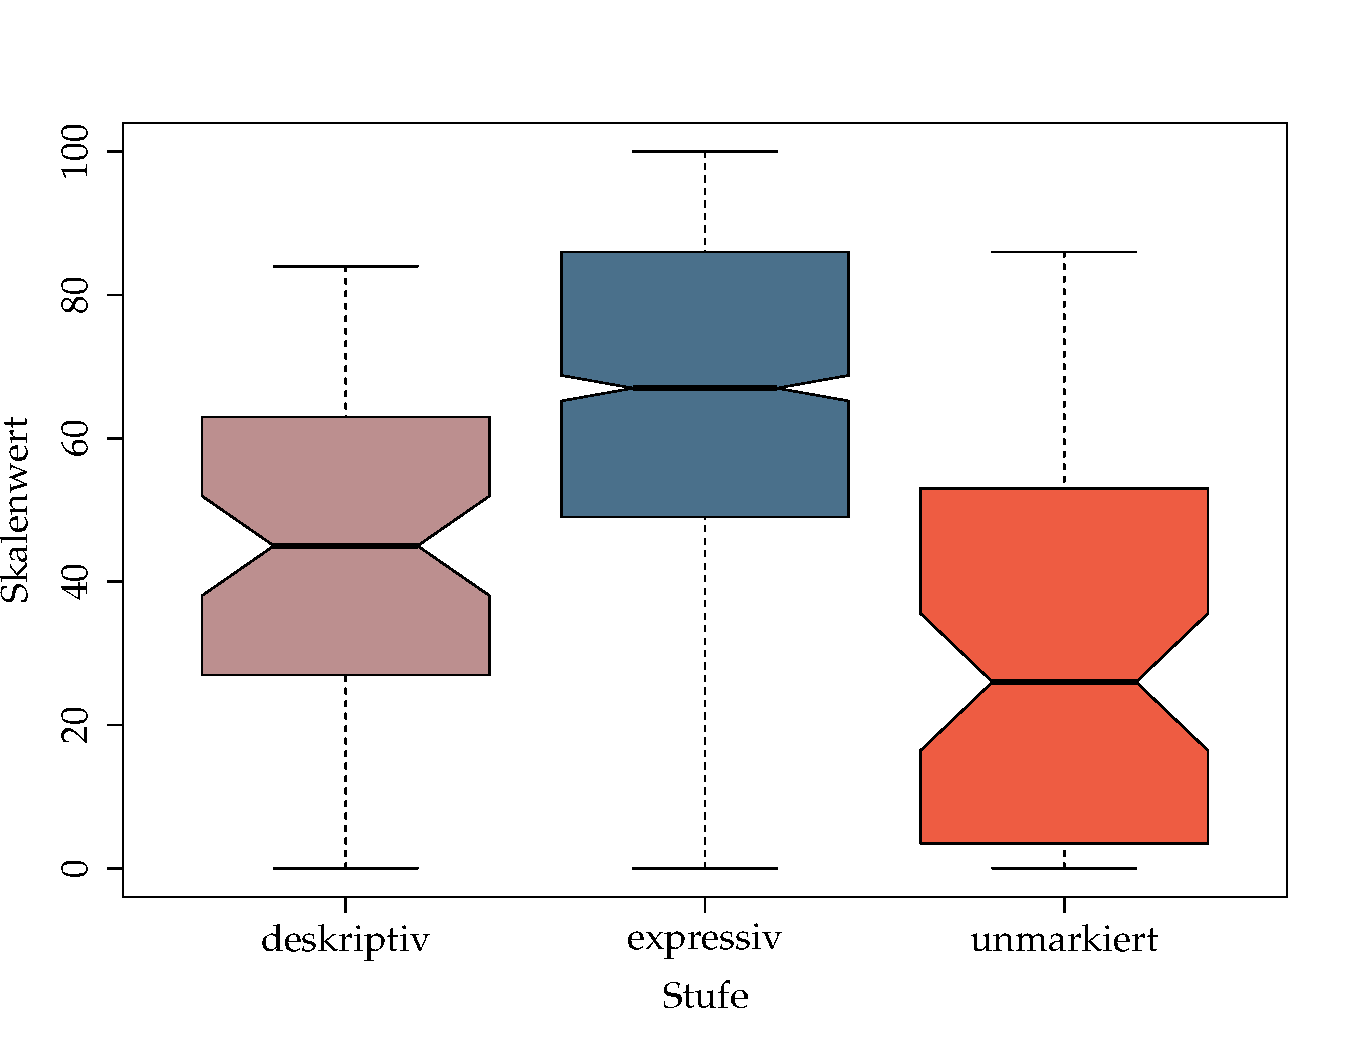
\includegraphics[width=1\textwidth]{BoxExpr_2}
	\caption[Gemittelte Skalenwerte der Stufen bei {Aufgabe II} von Experiment 1]{Gemittelte Skalenwerte der Stufen bei Aufgabe II -- Sprechereinstellung (x-Achse = Stufe, y-Achse = Skalenwert).}
  \label{ExpressivBox}
\end{figure}


\subsubsection{Regressionsanalysen zum Vergleich der Stufen}


Nachfolgend werden die Regressionsmodelle für Aufgabe II vorgestellt. Auch diese beruhen auf dem jeweiligen vollen Modell, das durch Rückwärtsselektion und \textit{anova}-Funktion nach und nach solange vereinfacht wurde, bis bloß noch signifikante Effekte darin enthalten waren. Das volle Regressionsmodell beinhaltete \textit{Fixed Effects} für den \textsc{Skalenwert} als metrische abhängige Variable sowie für die kategorialen Prädiktoren \textsc{Stufe} und \textsc{Position} sowie deren Zwei-Wege-Interaktionen. In dieser Aufgabe steht die Variable \textsc{Skalenwert} für den Grad an Sprechereinstellung, den die Versuchspersonen der jeweiligen Stufe bzw. dem jeweiligen Intensivierer zugesprochen haben. Um einen möglichen graduellen Effekt und Unterschiede zwischen den drei Stufen zu finden, wurde das Referenzlevel `Expressiv' jeweils mit {`Deskriptiv'} und `Unmarkiert' kontrastiert. Wie schon bei Skalarität geschah dies in Form von Dummy-Codierung, bei der die Ausprägungsformen der mehrkategorialen Variable \textsc{Stufe} in zwei Schritten als $0$ und $1$ kodiert und dadurch nach binären Kontrasten separiert wurden {\citep[vgl.][407,\,442]{Sauer.2019}}. Auf diese Weise wurden auch hier aus einer unabhängigen Variable mit drei Stufen zwei unabhängige Variablen mit je zwei Stufen. Außerdem fanden sich im vollen Modell versuchspersonen- und itemweise \textit{Random Intercepts} und \textit{Random Slopes} für die Variablen \textsc{Skalenwert}, \textsc{Stufe} und  \textsc{Position}. Das finale Regressionsmodell enthält signifikante Haupteffekte für den Prädiktor \textsc{Stufe}. Die berechneten Koeffizienten sind in {Tabelle \ref{LinReg0002}} zusammengetragen.

%
\begin{table}
%\setlength{\tabcolsep}{9.5pt}
\begin{tabularx}{\textwidth}{Xccccr}
\lsptoprule
Prädiktor & \textit{Est.} & \textit{SE} & \textit{$\chi$$^{2}$} & \textit{p} & \\
\midrule
(Intercept) & \textcolor{white}{-}65,38 & 2,26 & 126,18 & < 0,001 & $\star$$\star$$\star$\\
Expressiv vs. Deskriptiv & -22,75 & 3,26 & \textcolor{white}{-}36,86 & < 0,001 & $\star$$\star$$\star$ \\
Expressiv vs. Unmarkiert & -34,47 & 3,83 & \textcolor{white}{-}51,58 & < 0,001 & $\star$$\star$$\star$\\
\lspbottomrule
\end{tabularx}
\caption[Finales Regressionsmodell zu Aufgabe II von Experiment 1 (mit `Expressiv' als Referenzlevel)]{Finales Regressionsmodell zu Aufgabe II -- Sprechereinstellung (mit `Expressiv' als Referenzlevel).}
\label{LinReg0002}
\end{table}

\noindent Die in Tabelle \ref{LinReg0002} gezeigten Koeffizienten deuten darauf hin, dass sich die expressive Stufe bei Aufgabe II signifikant von den beiden anderen Stufen unterscheidet. So ist einerseits ein statistisch signifikanter Unterschied beim Vergleich der expressiven Stufe mit der deskriptiven Stufe zu verzeichnen ({$\chi$$^{2}$\,(1) = 36,86}, \textit{p} < 0,001). Andererseits unterscheiden sich die expressive und die unmarkierte Stufe ebenso signifikant voneinander ($\chi$$^{2}$\,(1) = 51,58, {\textit{p} < 0,001}). Dieser Befund stimmt im Wesentlichen mit der Annahme überein, dass Sätzen mit expressivem Intensivierer grundsätzlich ein höherer Grad an Sprechereinstellung zugeschrieben wird als Sätzen mit deskriptivem Intensivierer oder unintensivierten Sätzen.


Auch bei Aufgabe II wurde das Referenzlevel der mehrkategorialen Variable \textsc{Stufe} in einer weiteren Analyse auf `Unmarkiert' gesetzt, um zu überprüfen, inwiefern sich die unintensivierten Sätze in Hinsicht auf die ausgedrückte Sprechereinstellung von Sätzen mit deskriptivem oder expressivem Intensivierer unterscheiden. Erneut wurden ausgehend vom vollen Modell durch Rückwärtsselektion und Modellvergleich alle Effekte getilgt, die den Modell-Fit nicht signifikant verbesserten. Die \textit{Random-Effects}-Struktur entsprach mit Ausnahme des Referenzlevels der beiden binären Vergleiche der des obigen Modells. Das finale Modell beinhaltet signifikante Haupteffekte für den Prädiktor \textsc{Stufe}. Die berechneten Koeffizienten sind in {Tabelle \ref{LinReg0020} angegeben}.


\begin{table}
%\setlength{\tabcolsep}{10pt}
\begin{tabularx}{\textwidth}{Xccccr}
\lsptoprule
Prädiktor & \textit{Est.} & \textit{SE} & \textit{$\chi$$^{2}$} & \textit{p} & \\
\midrule
(Intercept) & 31,02 & 3,05 & 94,75 & < 0,001 & $\star$$\star$$\star$\\
Unmarkiert vs. Expressiv & 34,39 & 3,81 & 51,58 & < 0,001 & $\star$$\star$$\star$ \\
Unmarkiert vs. Deskriptiv & 11,63 & 3,01 & 13,08 & < 0,001 & $\star$$\star$$\star$\\
\lspbottomrule
\end{tabularx}
\caption[Finales Regressionsmodell zu Aufgabe II von Experiment 1 (mit `Unmarkiert' als Referenzlevel)]{Finales Regressionsmodell zu Aufgabe II -- Sprechereinstellung (mit `Unmarkiert' als Referenzlevel).}
\label{LinReg0020}
\end{table}


\noindent Die Werte in Tabelle \ref{LinReg0020} verdeutlichen, dass unintensivierte Sätze mit einem niedrigeren Grad an Sprechereinstellung assoziiert werden als mittels Intensivierer modifizierte Sätze. So zeigt sich beim Vergleich der unmarkierten Stufe mit der expressiven Stufe ein signifikanter Unterschied ($\chi$$^{2}$\,(1) = 51,58, \textit{p} < 0,001), ebenso wie der beobachtete Unterschied zwischen der unmarkierten Stufe und der deskriptiven Stufe signifikant ist ($\chi$$^{2}$\,(1) = 13,08, {\textit{p} < 0,001}).


Zusammengenommen bestätigen also auch die Ergebnisse der Datenauswertung von Aufgabe II den in der theoretischen Literatur postulierten Unterschied zwischen der deskriptiven und expressiven Intensiviererklasse (vgl. {\citealt[315]{Lang.1983}}; \citealt[57]{Ortner.2014}). So wurde der Grad an Sprechereinstellung bei Sätzen mit expressivem Intensivierer von den Versuchspersonen tatsächlich als signifikant höher eingeschätzt als der von Sätzen, die mit dem deskriptiven Intensivierer oder unintensiviert präsentiert wurden.





\subsubsection{Vergleich der Intensivierer} \label{abs:I-Vergleich513}


Um einen besseren Überblick über die Einschätzung der einzelnen Ausdrücke zu erhalten und Vergleichbarkeit zu gewährleisten, werden die gemittelten Skalenwerte und Standardabweichungen im Folgenden für Aufgabe II im Detail betrachtet. Diese Werte sind {Tabelle \ref{SkaWey}} zu entnehmen. Auch hier sind die expressiven Intensivierer in ansteigendem Skalenwert angeordnet.




\begin{table}
%\setlength{\tabcolsep}{26.25pt}
\begin{tabularx}{.8\textwidth}{Xlrr}
\lsptoprule
%       &  \multicolumn{1}{c}{\textbf{Aufgabe II}}          &  \\
%       &  \multicolumn{1}{c}{\textbf{Sprechereinstellung}} &  \\
Stufe & Intensivierer  & Skalenwert                       & \textit{SD}\\
\midrule
 \rowcolor[gray]{.90}
\multicolumn{1}{l}{deskriptiv} & \textit{sehr} &  42,34 &  23,3\\
 \multicolumn{1}{l}{expressiv} & \textit{arg}  &  56,94 &  24,6\\
  \rowcolor[gray]{.90}
 & \textit{voll}         & 59,61 &   23,7\\
 & \textit{wahnsinnig}   & 60,33 &   26,4\\
    \rowcolor[gray]{.90}
  & \textit{ober}        & 60,43 &   25,2\\
 & \textit{unheimlich}   & 60,94 &   24,9\\
  \rowcolor[gray]{.90}
 & \textit{derb}         & 62,63 &   22,5\\
   & \textit{hammer}     & 66,06 &   27,5\\
  \rowcolor[gray]{.90}
 & \textit{mega}         & 66,58 &   24,9\\
  & \textit{super}       & 66,60 &   23,5\\
  \rowcolor[gray]{.90}
  & \textit{furchtbar}   & 66,64 &   25,3\\
  & \textit{verdammt}    & 66,66 &   22,0\\
  \rowcolor[gray]{.90}
  & \textit{schrecklich} & 66,76 &   23,6\\
 & \textit{sau}          & 68,24 &   25,1\\
  \rowcolor[gray]{.90}
   & \textit{krass}      & 68,63 &   26,9\\
  & \textit{fürchterlich} & 68,75 &  22,3\\
  \rowcolor[gray]{.90}
 & \textit{scheiß}       & 78,12 &   25,0\\
\multicolumn{1}{l}{unmarkiert} & \textit{$\emptyset$} & 30,11 &  26,1\\
\lspbottomrule
\end{tabularx}
\caption[Gemittelte Skalenwerte der einzelnen Intensivierer bei Aufgabe II von Experiment 1]{Gemittelte Skalenwerte und Standardabweichungen der einzelnen Intensivierer bei Aufgabe II -- Sprechereinstellung (angeordnet nach ansteigendem Skalenwert der expressiven Intensivierer).}
\label{SkaWey}
\end{table}



Auch die in Tabelle \ref{SkaWey} präsentierten Werte deuten darauf hin, dass sich der Unterschied zwischen den Stufen stark vergrößert hat. Hier liegt der gemittelte Skalenwert des deskriptiven Intensivierers \textit{sehr} mit 42,34 Punkten weit unter den Werten der expressiven Intensivierer. Abgeschlagen dahinter befindet sich die unmarkierte Variante, der von den Versuchspersonen ein Skalenwert von durchschnittlich 30,11 Punkten zugewiesen wurde. Wieder ist das Skalenspektrum der expressiven Intensivierer recht eng gefasst: So liegt der niedrigste expressive Intensivierer \textit{arg} auf der Skala im Schnitt bei 56,94 Punkten, während \textit{scheiß} mit durchschnittlich 78,12 Punkten am höchsten positioniert wurde {($\Delta$ = ca. 21,20 Punkte)}. Auffällig ist, dass \textit{arg} neben Skalarität auch im Hinblick auf Sprechereinstellung als am niedrigsten bewertet wurde. Diese Tendenzen sind im Anhang \ref{Rat2} in Abbildung \ref{Expressiv7} in Form eines Säulendiagramms visualisiert. Im Anhang \ref{Pseu2} findet sich in {Tabelle \ref{Pseudos2}} ferner eine Übersicht der gemittelten Skalenwerte jeder Kombination aus Pseudonomen und Pseudoadjektiv. Darin ist zu verzeichnen, dass sich die Pseudowörter hinsichtlich ihrer Skaleneinschätzung ähnlich verhalten. Wurde der Kombination aus \textit{Der Cobe} und \textit{speiglich} mit durchschnittlich 58,75 Punkten von den Versuchspersonen der niedrigste Skalenwert zugeschrieben, weist die Kombination aus \textit{Die Itne} und \textit{schühnlich} mit durchschnittlich 65,34 Punkten den höchsten Skalenwert auf ({$\Delta$ = ca. 6,59 Punkte}). Auch hier legt die bloß geringe Differenz nahe, dass die Verwendung von Pseudowörtern einem Einfluss der semantischen Eigenschaften entgegengewirkt hat. Erneut sind die Skalenwerte der Pseudowörter zur besseren Anschaulichkeit im Anhang \ref{Happy4} in Abbildung \ref{Happy5} mittels Säulendiagramm {grafisch dargestellt}.





\subsubsection[Einfluss von Sprechereinstellung auf Skalarität]{Beeinflusst die Sprechereinstellung die Skalarität?}


Im Anschluss wird untersucht, ob zwischen der in Aufgabe I erfragten Skalarität und der in Aufgabe II erfragten Sprechereinstellung eine signifikante Korrelation besteht. In diesem Kontext ist gemäß der Definition von Expressivität nach \citet[133]{Gutzmann.2019a} vorstellbar, dass ein höherer Grad an Sprechereinstellung immer von einem höheren Grad an Skalarität begleitet wird. Wenn der Skalenwert der Variable \textsc{Sprechereinstellung} zunimmt, steigt in der Folge mutmaßlich auch der Skalenwert der Variable \textsc{Skalarität} an. Zur Quantifizierung des potenziellen linearen Merkmalszusammenhangs  wurde auf Basis der Mittelwerte der expressiven Intensivierer der Korrelationskoeffizient \textit{r} nach Pearson berechnet,\footnote{Die Produkt-Moment-Korrelation nach Pearson ist eine parametrische Methode, die als Zusammenhangsmaß den Korrelationskoeffizienten \textit{r} nimmt. Dabei handelt es sich um die Wurzel aus dem Bestimmtheitsmaß, die zwischen -$1$ ($\hateq$ negative Korrelation) und +$1$ {($\hateq$ positive Korrelation)} liegt. Je mehr sich der Wert $0$ annähert, desto geringer ist der Zusammenhang zwischen zwei Variablen. In diesem Fall spricht man von Unkorreliertheit (vgl. {\citealt[128ff.]{Mittag.2016}}; \citealt[89]{Winter.2020}).} dessen \textit{Estimate} wie folgt aussieht: {|\textit{r}| = 0,60}. Das Ergebnis des zugehörigen \textit{t}-Tests\footnote{Mithilfe des Hypothesentests \textit{t}-Test kann festgestellt werden, ob sich die Mittelwerte zweier abhängiger Stichproben signifikant voneinander unterscheiden \citep[vgl.][280f.]{Sauer.2019}.} ist signifikant ({\textit{t}\,(14) = 2,78}, \textit{p} < 0,05), was bedeutet, dass Skalarität und Sprechereinstellung im Experiment in der Tat in einer Korrelation stehen: Wenn der Grad an Sprechereinstellung von den Versuchspersonen als hoch empfunden wurde, wurde ebenso der Skalaritätsgrad auf der Skala höher verortet.


Ergänzend zur Korrelationsanalyse wurde ein lineares Regressionsmodell gerechnet, mit dessen Hilfe überprüft werden kann, ob der Grad an Sprechereinstellung im Experiment den Grad an Skalarität bedingte. Auch hier ist denkbar, dass die Skalarität mit steigender Sprechereinstellung zunimmt. Es wurde also getestet, ob die unabhängige Variable \textsc{Sprechereinstellung} einen signifikanten Effekt auf die abhängige Variable \textsc{Skalarität} hat. Das lineare Modell beinhaltet \textit{Fixed Effects} für die \textsc{Skalarität} und die \textsc{Sprechereinstellung}. Die berechneten Koeffizienten sind in {Tabelle \ref{LM01}} aufgeführt.


\begin{table}
%\setlength{\tabcolsep}{6.5pt}
\begin{tabularx}{\textwidth}{Xccccr}
\lsptoprule
Prädiktor & \textit{Est.} & \textit{SE} & \textit{F} & \textit{p} & \\
\midrule
(Intercept) & 24,52 & \textcolor{white}{-}7,03 & 12,15 & < 0,001 & $\star$$\star$$\star$\\
Skalarität vs. Sprechereinstellung & 66,38 & 11,18 & 35,22 & < 0,001 & $\star$$\star$$\star$\\
\lspbottomrule
\end{tabularx}
\caption[Lineares Regressionsmodell zum Einfluss von Sprechereinstellung auf Skalarität bei Experiment 1]{Lineares Regressionsmodell zum Einfluss von Sprechereinstellung auf Skalarität.}
\label{LM01}
\end{table}

\noindent Den Werten aus Tabelle \ref{LM01} nach hat die Sprechereinstellung tatsächlich einen signifikanten Einfluss auf die Skalarität ({$F$ = 35,22}, \textit{p} < 0,001). Demzufolge liegt es nahe, dass der Grad an Skalarität umso größer wird, desto höher der Grad an Sprechereinstellung ist. Dieser Befund stimmt mit der Annahme im Sinne von \citet[133]{Gutzmann.2019a} überein. Darüber, ob die Annahme, dass sich die Sprechereinstellung auf die Skalarität eines Ausdrucks auswirkt, grundsätzlich korrekt ist, macht das Modell jedoch keine Aussage.


Dieses Ergebnis ist in Abbildung \ref{Korr00} in Form einer linearen Regression visualisiert. Die Regressionslinie illustriert die vorhergesagte, geschätzte Sprechereinstellung der im Experiment berücksichtigten expressiven Intensivierer. Dabei zeigt sie den systematischen Zusammenhang zwischen Skalarität und Sprechereinstellung an, der sich hier durch eine Steigung ausdrückt. Die Tatsache, dass der Grad an Skalarität mit steigendem Grad an Sprechereinstellung zunimmt, belegt ebendiesen korrelativen Zusammenhang. 


\begin{figure}
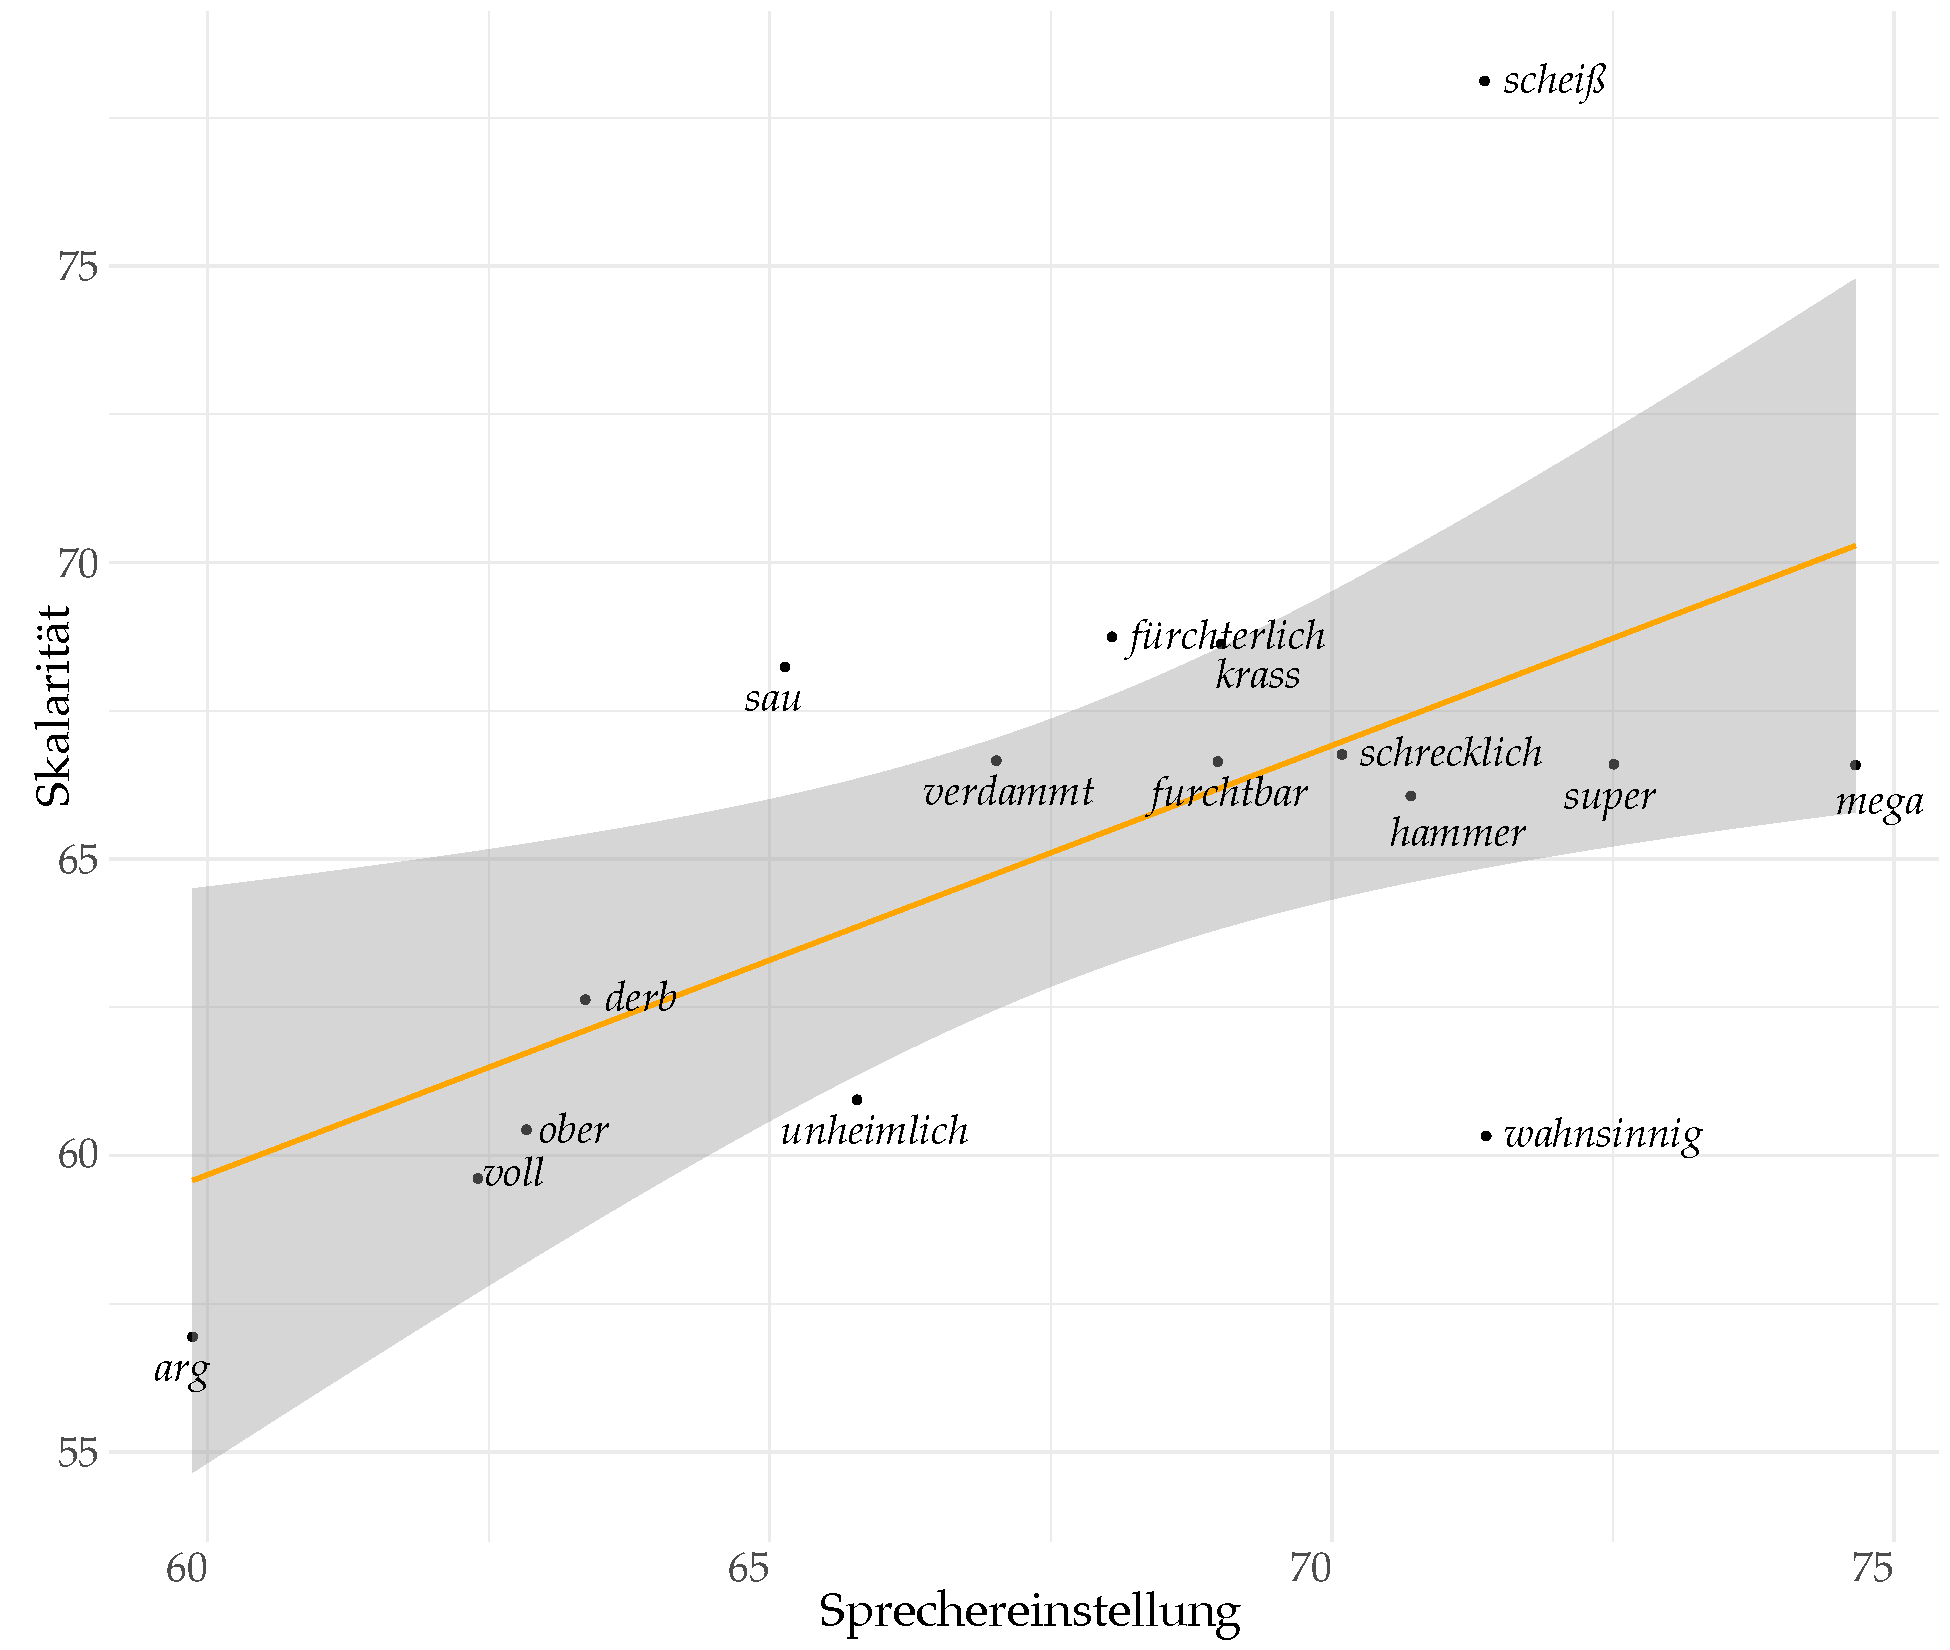
\includegraphics[width=\textwidth]{SkalExpr1}
\caption[Lineare Regression zum Einfluss von Sprechereinstellung auf Skalarität bei Experiment 1]{Lineare Regression zum Einfluss von Sprechereinstellung auf Skalarität (x-Achse = Sprechereinstellung, y-Achse = Skalarität).}
\label{Korr00}
\end{figure}






\subsubsection{Regressionsanalyse zu Frequenz und Persistenz}


Als Nächstes wird die in Aufgabe II erfragte Sprechereinstellung im Hinblick auf die oben erläuterten Frequenz- und Persistenzgruppen untersucht. Um dem möglichen Einfluss von Frequenz und Persistenz und somit der Gültigkeit der Hypothesen H1-Freq und H1-Temp nach {\citet[2]{Hauschild.1899}} und \citet[59]{Tobler.1868} auf den Grund zu gehen, wurden die durch die Korpusanalyse eingeteilten Gruppen im vollen Modell als Ausgangspunkt gewählt. Dieses wurde durch Rückwärtsselektion und Modellvergleich schrittweise vereinfacht, bis ausschließlich signifikante Effekte darin enthalten waren. Das volle Regressionsmodell beinhaltete \textit{Fixed Effects} für den \textsc{Skalenwert} als metrische abhängige Variable sowie für die kategorialen Prädiktoren \textsc{Frequenzgruppe}, \textsc{Persistenzgruppe} und \textsc{Position} sowie deren Zwei-Wege-Interaktionen. Um potenzielle Unterschiede zwischen hoch- und niedrigfrequenten Ausdrücken zu finden, wurde die binäre nominale Variable \textsc{Frequenzgruppe} dummy-gecoded, wobei der Stufe `Hoch' der {Wert $0$} und der Stufe `Niedrig' der Wert $1$ zugewiesen wurde. Auch wurde die binäre nominale Variable \textsc{Persistenzgruppe} dummy-gecoded. Im Zuge dessen wurde die Stufe `Alt' als $0$ und die Stufe `Neu' als $1$ codiert. Diese Stufen wurden anschließend jeweils miteinander verglichen. Außerdem wurden im vollen Modell versuchspersonenweise \textit{Random Intercepts} und \textit{Random Slopes} für die Variablen  \textsc{Skalenwert}, \textsc{Frequenzgruppe}, \textsc{Persistenzgruppe} und \textsc{Position} miteingerechnet und dadurch eventuelle Unterschiede zwischen den Versuchspersonen berücksichtigt.\footnote{Da das volle Regressionsmodell unter Einbezug der Pseudowörter nicht konvergierte, konnten bei dieser Berechnung lediglich versuchspersonenweise \textit{Random Intercepts} und \textit{Random Slopes} miteingebunden werden.} Das finale Regressionsmodell enthält einen signifikanten Haupteffekt für den Prädiktor \textsc{Frequenzgruppe}. Die berechneten Koeffizienten der Regressionsanalyse befinden sich in {Tabelle \ref{LinRegzaz0}}.

%
\begin{table}
%\setlength{\tabcolsep}{14pt}
\begin{tabularx}{.8\textwidth}{Xccccr}
\lsptoprule
Prädiktor & \textit{Est.} & \textit{SE} & \textit{$\chi$$^{2}$} & \textit{p} & \\
\midrule
(Intercept) & 63,55 & 2,34 & 2,17 & < 0,001 & $\star$$\star$$\star$\\
Hoch vs. Niedrig & \textcolor{white}{-}3,01 & 1,06 & 7,97 & < 0,01 & \multicolumn{1}{r}{$\star$$\star$} \\
\lspbottomrule
\end{tabularx}
\caption[Finales Regressionsmodell zu Aufgabe II von Experiment 1 (Frequenz mit `Hoch' als Referenzlevel)]{Finales Regressionsmodell zu Aufgabe II -- Sprechereinstellung (Frequenz mit `Hoch' als Referenzlevel).}
\label{LinRegzaz0}
\end{table}

\noindent Die in Tabelle \ref{LinRegzaz0} gesammelten Koeffizienten liefern Bestätigung für die Hypothese, dass eine hohe Frequenz zu einem als niedriger eingeschätzten Grad an Sprechereinstellung führt, unterscheiden sich die beiden Frequenzgruppen dahingehend doch signifikant voneinander ({$\chi$$^{2}$\,(1) = 7,97}, \textit{p} < 0,01). Dementsprechend werden die hochfrequenten Intensivierer grundsätzlich mit einem niedrigeren Grad an Sprechereinstellung assoziiert als die niedrigfrequenten Intensivierer. Mit anderen Worten: Bei einem Wechsel von `Hochfrequent' nach `Niedrigfrequent' nimmt der wahrgenommene Grad an Sprechereinstellung deutlich zu. Nachweislich keinen Einfluss auf die Einschätzung des Grades an Sprechereinstellung hat dagegen die Persistenz. Dieser Befund wird weiter unten in {Abschnitt \ref{abs:Diskussion22}} ausführlich besprochen.


Insgesamt untermauern die Ergebnisse der Regressionsanalyse die {Hypothese H1-Freq} nach \citet[2]{Hauschild.1899}. So wurden die im Korpus hochfrequenten Intensivierer von den Versuchspersonen mit einem bedeutend niedrigeren Grad an Sprechereinstellung assoziiert als die niedrigfrequenten Intensivierer. Dagegen findet sich keine empirische Evidenz, die die Gültigkeit der Hypothese H1-Temp nach \citet[59]{Tobler.1868} belegt. Aus welchem Grund dieses Resultat nur eingeschränkt aussagekräftig ist, wird ebenso in {Abschnitt \ref{abs:Diskussion22}} detailliert dargelegt.






\subsection{Aufgabe III -- Einstellungspolarität} \label{abs:Ev-Vergleich}
%Im nächsten Abschnitt werden die Resultate der in Aufgabe III ermittelten Einstellungspolarität präsentiert. Bei dieser Aufgabe ging es für die Versuchspersonen darum, mithilfe 100 virtueller Taler auf die evaluative Haltung zu setzen, die der Sprecher zum bezeichneten Sachverhalt hat. Dies diente der Beantwortung der Frage, ob expressive Intensivierer eine als positiv oder negativ wahrgenommene Interpretation der Sprechereinstellung nach sich ziehen. Vor diesem Hintergrund ist bspw. vorstellbar, dass Intensivausdrücke, die Mitglieder der \glqq{}schrecklichen\grqq{} Intensivierergruppe beinhalten, von den Versuchspersonen als verstärkt negativ beurteilt werden, wohingegen das semantisch entleerte \textit{sehr} möglicherweise zu einer als neutral wahrgenommenen Sprechereinstellung führt. Ob diese Mutmaßung durch die Ergebnisse der Untersuchung gestützt wird, wird im Anschluss erörtert.






\subsubsection{Vergleich der Stufen} \label{abs:VP-Vergleich636}


Im ersten Schritt werden die Mittelwerte der gesetzten Taler und Standardabweichungen für die drei Stufen mit Blick auf die Einstellungspolarität begutachtet. Diese Werte befinden sich in Tabelle \ref{Bedin}. Wiederholt werden die expressiven Intensivierer zunächst zu einer Stufe zusammengefasst. In der Tabelle ist jeweils diejenige Spalte farblich hervorgehoben, deren Stufe die Versuchspersonen die höchste Anzahl von Talern zugewiesen haben.

%
\begin{table}
%\setlength{\tabcolsep}{24.5pt}
\begin{tabularx}{\textwidth}{X rr rr rr}
\lsptoprule
%  & \multicolumn{3}{c}{\textbf{Aufgabe III}}  \\
% \multirow{2}{*}{Stufe}  & \multicolumn{3}{c}{\textbf{Einstellungspolarität}}  \\ [0.5em]
  & \multicolumn{2}{c}{ {positiv}} & \multicolumn{2}{c}{ {neutral}} & \multicolumn{2}{c}{ {negativ}} \\
  \cmidrule(lr){2-3}\cmidrule(lr){4-5}\cmidrule(lr){6-7}
   & Taler  &  SD& Taler  &  SD& Taler  &  SD\\
\midrule
{deskriptiv} & 30,60 & 24,5   & \cellcolor[gray]{.90}46,37 & \cellcolor[gray]{.90}29,3    &   23,03 & 23,5 \\
{expressiv} & 32,03 & 29,5   & 27,34 & 26,2   &   \cellcolor[gray]{.90} 40,63 & \cellcolor[gray]{.90}32,3 \\
{unmarkiert} & 22,34  & 27,4  & \cellcolor[gray]{.90}62,05 & \cellcolor[gray]{.90}33,7   &   15,61 & 20,6 \\
\lspbottomrule
\end{tabularx}
\caption[Mittel der gesetzten Taler der Stufen bei {Aufgabe III} von Experiment 1]{Mittel der gesetzten Taler und Standardabweichungen der Stufen bei Aufgabe III -- Einstellungspolarität (Talersumme je Stufe = 100).}
\label{Bedin}
\end{table}


%
\noindent Die in Tabelle \ref{Bedin} gelisteten Werte weisen auf den ersten Blick darauf hin, dass sich die expressive Stufe grundlegend von den beiden anderen abhebt: Während Sätze der unmarkierten und deskriptiven Stufe vornehmlich als neutral eingeschätzt wurden, wurden Sätze mit expressivem Intensivierer dagegen verstärkt als negativ evaluiert. Das starke Übergewicht zugunsten der Abweichung von `Neutral' bei der expressiven Stufe lässt sich auch dadurch erkennen, indem man den Wert von `Neutral' mit dem der Abweichung, also der Summe aus `Positiv' und `Negativ', kontrastiert. Hier ergibt sich hinsichtlich `Neutral' vs. `Davon abweichend' bei der deskriptiven Stufe ein Verhältnis von 46,37 Talern zu 53,63 Talern, das sich als relativ ausbalanciert bezeichnen lässt. Die unmarkierte Stufe zeigt dahingehend ein Verhältnis von 62,05 Talern zu 37,95 Talern. Dies deutet darauf hin, dass die Sprechereinstellung bei unintensivierten Sätzen tendenziell vermehrt als neutral wahrgenommen wird. Bei der expressiven Stufe beträgt das Verhältnis hingegen 27,34 Taler zu 72,66 Taler, was bedeutet, dass die Sprechereinstellung bei expressiven Intensivierern stärker als positiv oder negativ bewertet wurde. Die beobachtete negative Tendenz hängt unter Umständen mit der Semantik der Ursprungslexeme zusammen, verfügt eine Vielzahl der untersuchten expressiven Ausdrücke doch über einen transparenten negativen Ursprung und eine ebensolche Konnotation (bspw. \textit{furchtbar} oder \textit{scheiß}). Im Unterschied dazu ist der Anteil an Ausdrücken mit klar erkennbarer positiver Herkunft oder Konnotation deutlich geringer (bspw. \textit{mega} oder \textit{super}).




\subsubsection{Regressionsanalyse zum Vergleich der Stufen} \label{abs:VP-Vergleich669}


Dieser Abschnitt widmet sich der Regressionsanalyse zu Aufgabe III. 
% Diese Aufgabe erfragte mithilfe einer Konstant-Summen-Skala die Polarität der Sprechereinstellung. Vor diesem Hintergrund wurde im Zusammenhang mit der Hypothese H3 angenommen, dass sich die Semantik des Ursprungslexems auf die Einschätzung der Polarität einwirkt, wenn der Intensivierer mit einem semantisch leeren Pseudowort kombiniert wird. Insofern stellt sich die Frage, ob die wahrgenommene Skalarität und Sprechereinstellung der Ausdrücke Einfluss auf ebendiese Einschätzung nehmen.
%Vor diesem Hintergrund wurde angenommen, dass diejenigen Intensivierer, die mit einem hohen Grad an Skalarität und Sprechereinstellung verbunden sind, eine stärkere Abweichung von 'neutral' hervorrufen als diejenigen, die jeweils mit einem niedrigeren Grad einhergehen. 
Das oben beschriebene statistische Vorgehen fand hier ebenfalls Anwendung. Wiederholt wurde zunächst ein volles Modell berechnet, das per Rückwärtsselektion und \textit{anova}-Funktion Schritt für Schritt vereinfacht wurde, bis alle Effekte getilgt waren, die den Modell-Fit nicht signifikant verbesserten. Das volle Modell enthielt \textit{Fixed Effects} für die \textsc{Einstellungspolarität}, die \textsc{Skalarität}, die \textsc{Sprechereinstellung}, die \textsc{Position} sowie deren Zwei-Wege-Interaktionen. Als Referenzlevel der abhängigen Variable \textsc{Einstellungspolarität}, die die drei Stufen `Positiv', `Neutral' und `Negativ' umfasst, wurde `Neutral' gewählt, d.\,h., es wurde überprüft, inwiefern die \textit{Fixed Effects} zu einer Abweichung -- ganz gleich, ob positiv oder negativ -- von ebendiesem neutralen Punkt führten. Die Abweichung von `Neutral' bzw. die Stufen `Positiv' und `Negativ' wurden mittels Dummy-Codierung zu einer Stufe zusammengefasst. Dabei wurde ihnen der Wert $1$ und der Stufe `Neutral' der Wert $0$ zugewiesen. Dieses Coding-Schema erlaubt es im Modell, den Grad an Abweichung von der neutralen Interpretation zu quantifizieren. Neben den \textit{Fixed Effects}  wurden im vollen Modell versuchspersonen- und itemweise \textit{Random Intercepts} und \textit{Random Slopes} für die Variablen \textsc{Einstellungspolarität}, \textsc{Skalarität}, \textsc{Sprechereinstellung} und \textsc{Position} miteingerechnet. Das finale Modell beinhaltet Haupteffekte für die Prädiktoren \textsc{Sprechereinstellung}, \textsc{Skalarität} und \textsc{Position}. Die berechneten Koeffizienten {Tabelle \ref{LinReg0004}} zu entnehmen.

%
\begin{table}
%\setlength{\tabcolsep}{11.5pt}
%\begin{tabular}{p{0.425\textwidth} p{0.1\textwidth} p{0.1\textwidth} p{0.1\textwidth}p{0.1\textwidth} p{0.05\textwidth}}
\begin{tabularx}{.8\textwidth}{Xccccr}
\lsptoprule
Prädiktor & \textit{Est.} & \textit{SE} & \textit{$\chi$$^{2}$} & \textit{p} & \\
\midrule
(Intercept) & \textcolor{white}{-}66,17 & 3,51 & 111,50 & < 0,001 & $\star$$\star$$\star$\\
Sprechereinstellung & -41,19 & 5,27 & \textcolor{white}{-}39,67 & < 0,001 & $\star$$\star$$\star$ \\
Skalarität & -14,03 & 4,77 & \textcolor{white}{-}\textcolor{white}{-}9,25 & < 0,01 & $\star$$\star$\\ 
Position & \textcolor{white}{-}\textcolor{white}{-}-1,35 & 0,65 & \textcolor{white}{-}\textcolor{white}{-}4,11 & < 0,05 & $\star$\\
\lspbottomrule
\end{tabularx}
\caption[Finales Regressionsmodell zu Aufgabe III von Experiment 1 (mit `Neutral' als Referenzlevel)]{Finales Regressionsmodell zu Aufgabe III -- Einstellungspolarität (mit `Neutral' als Referenzlevel).}
\label{LinReg0004}
\end{table}

\noindent Den in Tabelle \ref{LinReg0004} aufgeführten Werten nach werden Intensivierer, die mit einem hohen Grad an Sprechereinstellung assoziiert werden, von den Versuchspersonen als signifikant positiver oder negativer wahrgenommen ($\chi$$^{2}$\,(1) = 39,67, \textit{p} < 0,001). Ähnliches trifft auf Intensivierer zu, denen eine hohe Skalarität zugeschrieben wird ($\chi$$^{2}$\,(1) = 9,25, \textit{p} < 0,01). Demzufolge führt ein hoher Grad an Sprechereinstellung oder Skalarität zu einer von `Neutral' abweichenden Einschätzung der Sprechereinstellung -- völlig egal, ob positiv oder negativ. Ein weiterer signifikanter Effekt geht mit der \textsc{Position} einher ($\chi$$^{2}$\,(1) = 4,11, {\textit{p} < 0,05}). Somit wird der Grad der Abweichung von `Neutral' umso stärker eingeschätzt, je fortgeschrittener die Position eines Items im Experiment ist.


Es lässt sich zusammenfassen, dass die Ergebnisse der Datenauswertung von Aufgabe III den in der Literatur vertretenen Unterschied zwischen der deskriptiven und expressiven Intensiviererklasse stützen (vgl. {\citealt[135]{Gutzmann.2019a}}). Je höher der Grad an Skalarität und Sprechereinstellung eines Intensivierers empfunden wurde, desto stärker tendierten die Versuchspersonen zu einer als evaluativ eingeschätzten {Sprechereinstellung}.




\subsubsection{Vergleich der Einstellungspolarität} \label{abs:VP-Vergleich700}



\noindent Tabelle \ref{ValenzInten} bildet den Mittelwert der gesetzten Taler und die Standardabweichung je Intensivierer ab und ermöglicht eine genauere Inspektion der den Ausdrücken zugewiesenen Einstellungspolarität. Die expressiven Intensivierer sind zur besseren Übersicht nach ansteigendem negativen Skalenwert angeordnet.




%
\begin{table}
%\setlength{\tabcolsep}{7pt}
\fittable{
\begin{tabularx}{\textwidth}{Xlrrrrrr}
\lsptoprule
% \textbf{Aufgabe III} &  &  &  & & & & \\
% \textbf{Einstellungspolarität} &  &  &  & & & & \\
\multirow{2}{*}{Stufe} & \multirow{2}{*}{Intensivierer} &  &  & & & & \\
 & & \multicolumn{2}{c}{ {positiv}} & \multicolumn{2}{c}{ {neutral}} & \multicolumn{2}{c}{ {negativ}} \\
  \cmidrule(lr){3-4}\cmidrule(lr){5-6}\cmidrule(lr){7-8}
 &  & Taler            & \textit{SD} &  Taler            & \textit{SD} &  Taler           &\textit{SD}\\
\midrule
 \rowcolor[gray]{.90}
deskriptiv & \textit{sehr}   &  30,60 & 24,5 & 46,37 &  29,3 & 23,03 &  23,5\\
expressiv  & \textit{hammer} &  53,87 & 35,4 & 25,34 &  28,1 & 20,79 &  24,1\\
  \rowcolor[gray]{.90}
           & \textit{super}  &  50,42 & 31,1 & 25,67 &  26,0 & 23,91 &  25,9\\
           & \textit{mega}   &  49,58 & 31,6 & 23,30 &  26,4 & 27,12 &  26,9\\
  \rowcolor[gray]{.90}
           & \textit{ober}   &  36,46 & 28,6 & 33,23 &  28,6 & 30,31 &  28,5\\
       & \textit{wahnsinnig} &  38,00 & 29,0 & 31,39 &  29,2 & 30,61 &  27,9\\
  \rowcolor[gray]{.90}
       & \textit{unheimlich} &  31,55 & 26,5 & 34,84 &  27,4 & 33,61 &  28,0\\
             & \textit{voll} &  33,18 & 26,3 & 32,07 &  26,1 & 34,75 &  25,6\\
  \rowcolor[gray]{.90}
            & \textit{krass} &  34,43 & 25,8 & 28,99 &  26,0 & 36,58 &  28,2\\
            & \textit{sau}   &  33,57 & 28,5 & 27,52 &  27,1 & 38,91 &  29,0\\
  \rowcolor[gray]{.90}
            & \textit{derb}  &  25,42 & 23,2 & 31,07 &  26,6 & 43,51 &  31,1\\
        & \textit{verdammt}  &  28,60 & 28,1 & 27,60 &  23,4 & 43,80 &  29,7\\
  \rowcolor[gray]{.90}
              & \textit{arg} &  23,19 & 21,9 & 31,03 &  26,3 & 45,78 &  28,7\\
      & \textit{schrecklich} &  22,40 & 28,8 & 21,93 &  22,9 & 55,67 &  34,0\\
  \rowcolor[gray]{.90}
        & \textit{furchtbar} &  19,89 & 24,7 & 23,24 &  21,5 & 56,87 &  34,6\\
     & \textit{fürchterlich} &  15,12 & 19,0 & 24,57 &  25,1 & 60,31 &  33,6\\
  \rowcolor[gray]{.90}
           & \textit{scheiß} &  16,76 & 26,4 & 15,67 &  23,5 & 67,57 &  35,3\\
\multicolumn{1}{l}{unmarkiert} & \textit{$\emptyset$} &  22,34 & 27,4 & 62,05 &  33,7 & 15,61 &  20,6\\
\lspbottomrule
\end{tabularx}
}
\caption[Mittel der gesetzten Taler der einzelnen Intensivierer bei Aufgabe III von Experiment 1]{Mittel der gesetzten Taler und Standardabweichungen der einzelnen Intensivierer bei Aufgabe III -- Einstellungspolarität (Talersumme je Intensivierer = 100; angeordnet nach ansteigendem negativen Skalenwert).}
\label{ValenzInten}
\end{table}


\noindent Die Übersicht in Tabelle \ref{ValenzInten} erhärtet die in Bezug auf Tabelle \ref{Bedin} dargelegte Vermutung: Während der opake deskriptive Intensivierer \textit{sehr} und unintensivierte Sätze von den Versuchspersonen überwiegend als neutral eingestuft wurden, ist bei Intensivierern mit klar negativem Ursprung eine ausgeprägte Tendenz für die negative Polarität festzustellen (bspw. \textit{fürchterlich}, \textit{schrecklich} und \textit{scheiß}). Dies zeigt sich in acht von 18 Fällen ($\hateq$ 44,44\,\%): \textit{arg}, \textit{derb}, \textit{furchtbar}, \textit{fürchterlich}, \textit{sau}, \textit{scheiß}, \textit{schrecklich} und \textit{verdammt}. In fünf Fällen ist dagegen eine Tendenz in Richtung `Positiv' zu erkennen ($\hateq$ 27,78\,\%): \textit{hammer}, \textit{mega}, \textit{ober}, \textit{super} und \textit{wahnsinnig}. Eine Tendenz in Richtung `Neutral' kristallisiert sich in zwei Fällen heraus ($\hateq$ 11,11\,\%): bei \textit{sehr} und der unmarkierten Variante. Daneben weisen drei Fälle ein vorwiegend ausgewogenes Verhältnis {auf {($\hateq$ 16,67\,\%)}}: \textit{krass}, \textit{unheimlich} und \textit{voll}. Dieses Ergebnis deutet darauf hin, dass die Interpretation der Sprechereinstellung bei expressiven Intensivierern -- anders als beim deskriptiven Intensivierer oder der unmarkierten Variante des Satzes -- vermehrt als positiv oder negativ beurteilt wurde. Zur  Visualisierung sind die Mittelwerte der gesetzten Taler für jeden Intensivierer in Abbildung \ref{Aufg3.1} in Form von Säulendiagrammen dargestellt. Zusätzlich ist im Anhang \ref{Pseu3} in Tabelle \ref{Pseudos3} eine Übersicht über die gemittelten Taler je Kombination aus Pseudonomen und Pseudoadjektiv beigefügt

\begin{figure}
  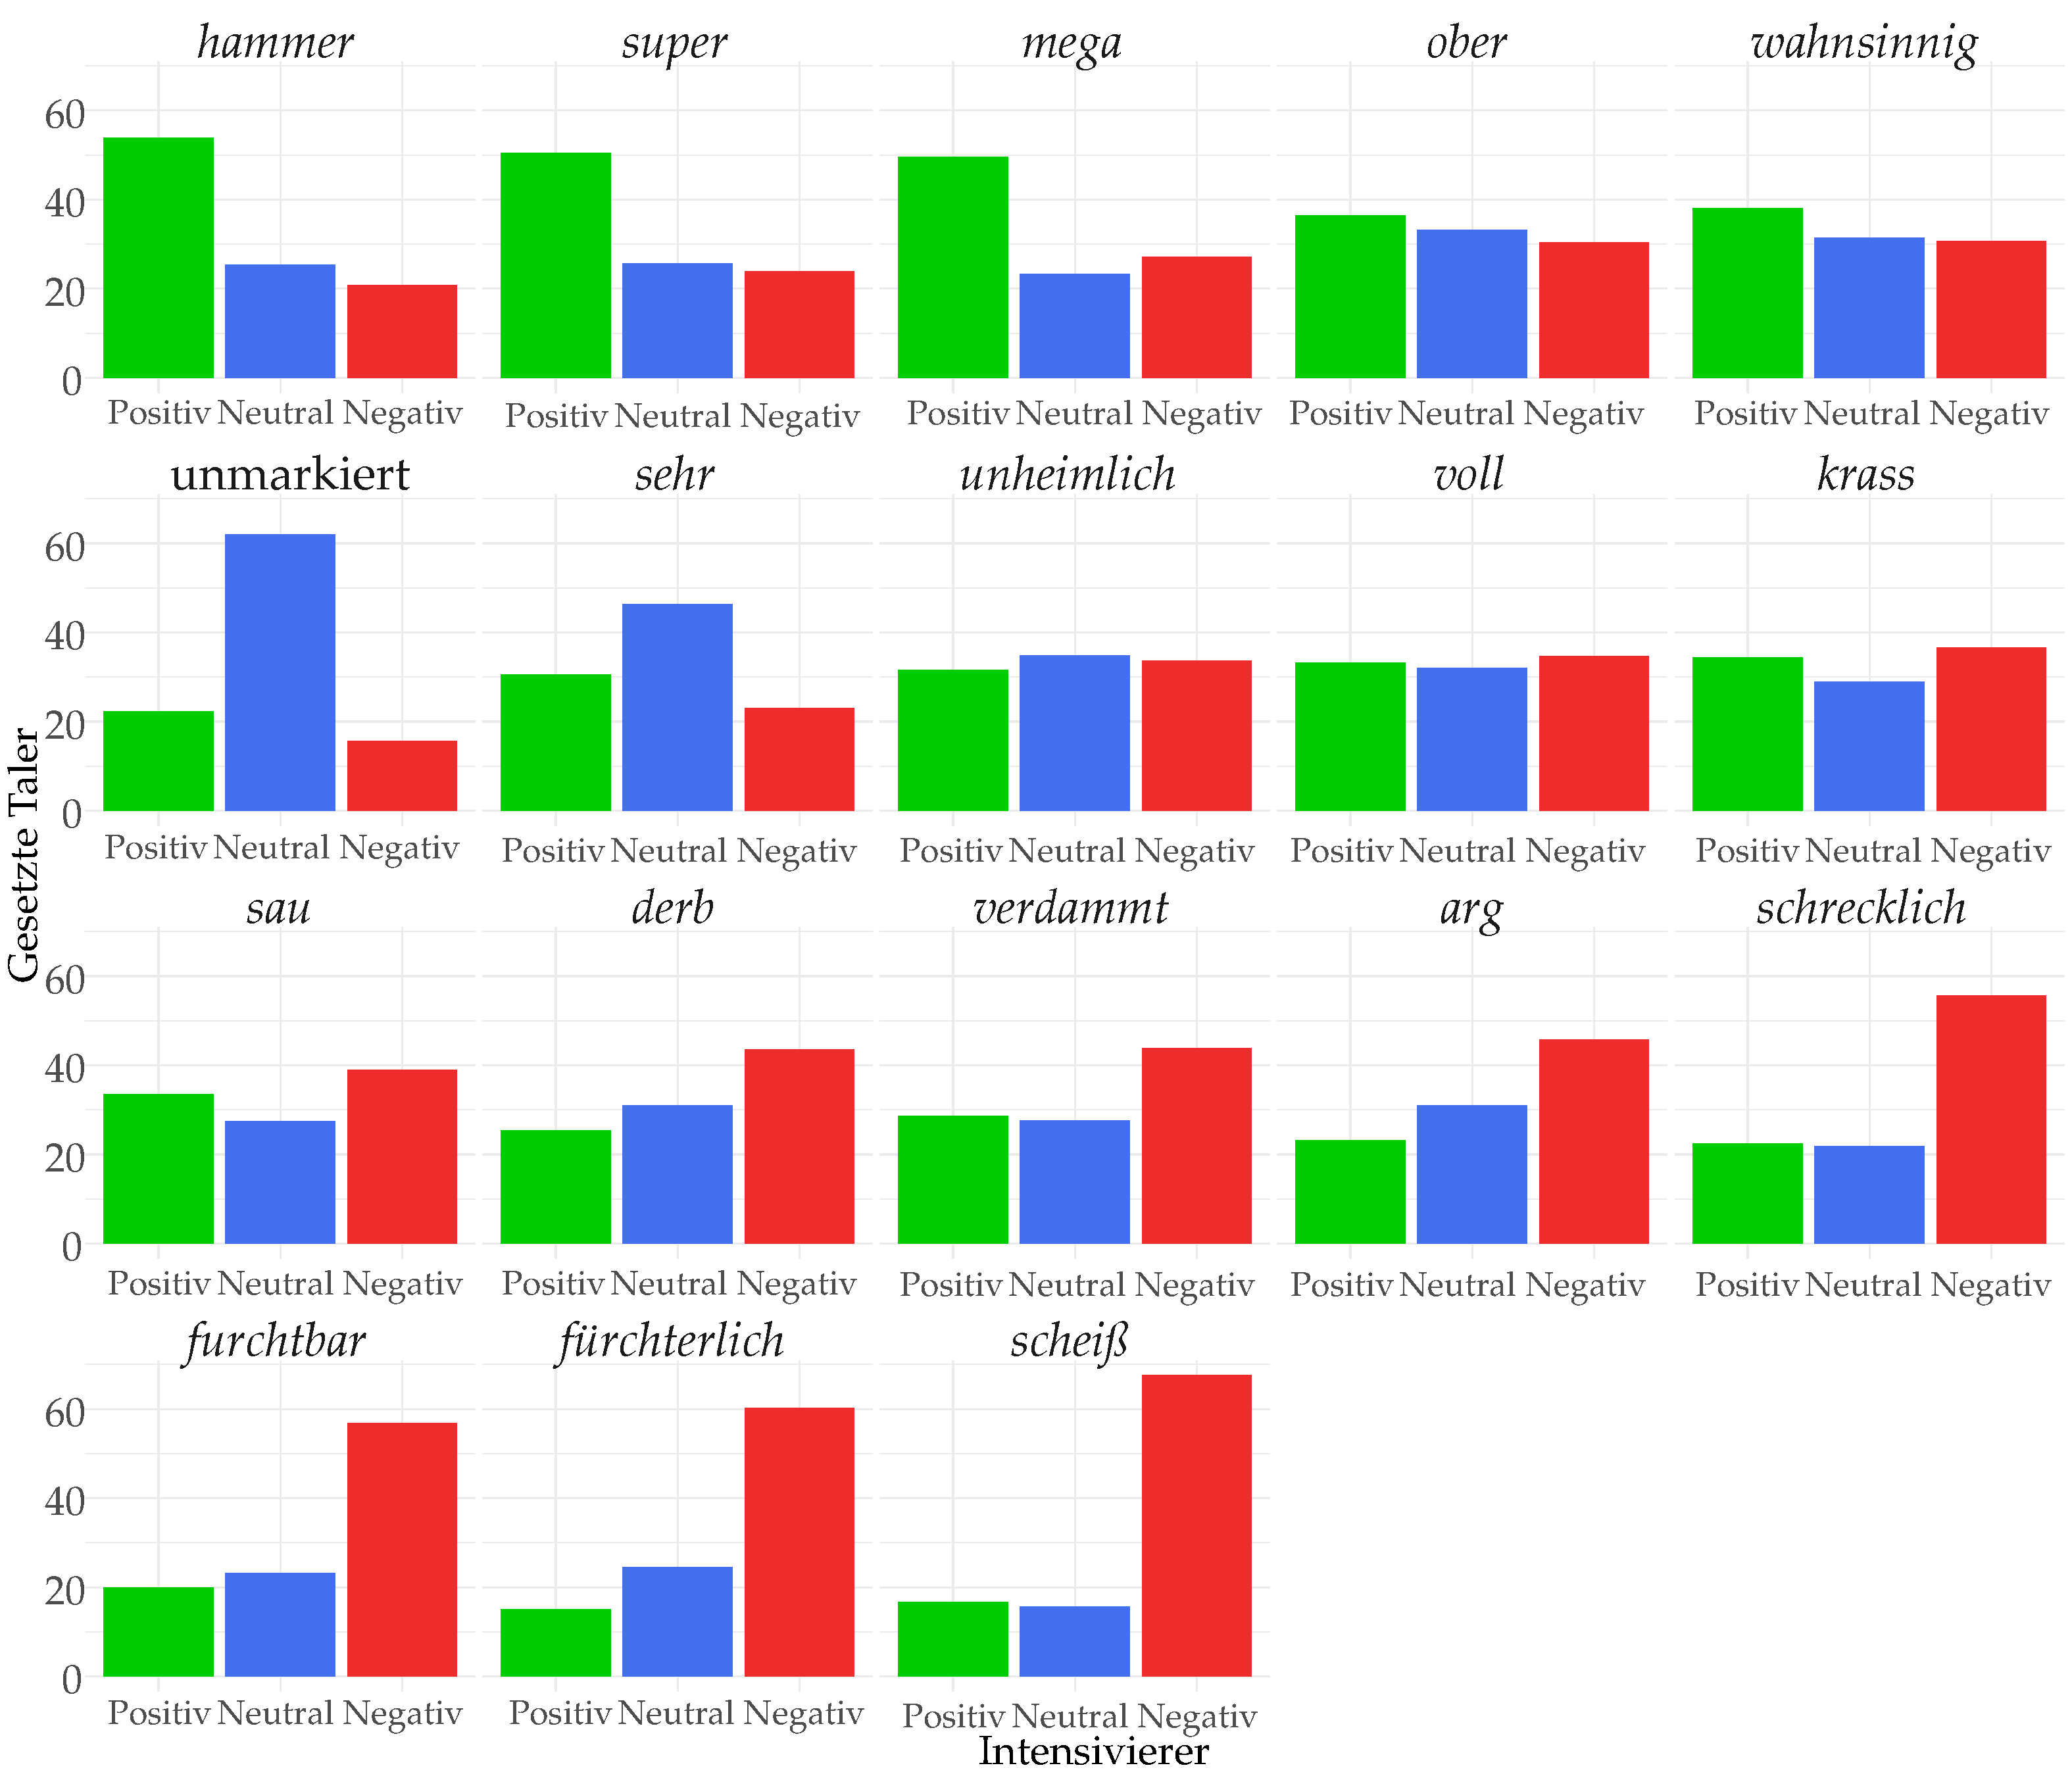
\includegraphics[width=0.975\textwidth]{Bewertung3_new}
	\caption[Säulendiagramme zu den Mitteln der gesetzten Taler je Intensivierer bei Aufgabe III von Experiment 1]{Säulendiagramme zu den Mitteln der gesetzten Taler je Intensivierer bei Aufgabe III -- Einstellungspolarität (x-Achse = Einstellungspolarität, y-Achse = Skalenwert).}
  \label{Aufg3.1}
\end{figure}


%Zusätzlich ist im Anhang \ref{Pseu3} in Tabelle \ref{Pseudos3} eine Übersicht über die gemittelten Taler je Kombination aus Pseudonomen und Pseudoadjektiv beigefügt. 
%Darin ist auszumachen, dass zwölf der insgesamt 18 Pseudowörter vermehrt in Richtung 'negativ' tendierten ($\hat{=}$ 66,67\,\%). Somit wurde die Mehrheit der Pseudowort-Kombinationen aufgrund des Intensivierers \textit{de facto} als von 'neutral' abweichend beurteilt. In Anbetracht der Menge an Intensivierern mit negativem Ursprung ist dieser Befund nicht sonderlich überraschend.



\section{Diskussion}\label{abs:Diskussion22}
Das dargelegte Experiment wurde einerseits mit dem Ziel durchgeführt, Rückschlüsse auf die noch ungeklärten Hypothesen aus der Korpusstudie ziehen zu können. Gemäß der Hypothese H1-Freq im Sinne von {\citet[2]{Hauschild.1899}} wirkt sich ein frequenter Gebrauch von Intensivierern negativ auf ihre Expressivität aus, die in der Konsequenz schwindet. Nach {\citet[59]{Tobler.1868}} spielt dabei jedoch auch der Faktor Zeit eine Rolle, erstreckt sich die Abnutzung von Intensivierern doch womöglich über eine gewisse Zeitspanne hinweg. Diese Annahme wurde in der Hypothese {H1-Temp} aufgegriffen. Andererseits wurden auch die {Hypothesen H3 und H4} auf ihre Richtigkeit hin überprüft, nach denen Expressivität gleichermaßen mit einem höheren Grad an Skalarität und Sprechereinstellung einhergeht, wie {\citet[22]{Paradis.1997}} und {\citet[133]{Gutzmann.2019a}} sowie {\citet[315]{Lang.1983}} und {\citet[57]{Ortner.2014}} anführen. Im Kontext der {Hypothese H5} wurde außerdem getestet, ob die Sprechereinstellung, die expressive Intensivierer mutmaßlich kommunizieren, evaluativ ist und vom Adressaten daher als positiv oder negativ interpretiert wird, wie {\citet[135]{Gutzmann.2019a}} ferner ergänzt.


Im Folgenden werden die im vorangegangenen Abschnitt präsentierten Untersuchungsergebnisse zusammengefasst und mit Blick auf die zentralen Hypothesen evaluiert. Dies geschieht in der Reihenfolge, in der die Merkmale Skalarität, Sprechereinstellung und Einstellungspolarität im Experiment berücksichtigt wurden. Darüber hinaus werden auch die Ergebnisse zur Rolle von Frequenz und Persistenz aufgearbeitet und besprochen.




\subsection{Aufgabe I -- Skalarität}
In Aufgabe I ging es für die Versuchspersonen darum, auf einer Skala von `normal' bis `maximal' anzugeben, wo sich der Grad der Eigenschaft des beschriebenen Objekts befindet. Die Fragestellung war im Wortlaut an den Itemsatz angepasst, z.\,B. \textit{Wie fongig ist der Nümig?} Die Idee dahinter bestand nach H3 darin, dass Sätze mit expressivem Intensivierer vermutlich einen höheren Grad an Skalarität ausdrücken als Sätze mit deskriptivem Intensivierer oder unintensivierte Sätze (vgl. {\citealt[22]{Paradis.1997}}; {\citealt[133]{Gutzmann.2019a})}. Um die durch die Untersuchung gewonnenen Daten auf ihre statistische Signifikanz hin zu überprüfen, wurden mithilfe von R lineare gemischte Modelle berechnet, die aus der unabhängigen Variable die abhängige Variable voraussagen.


Die Ergebnisse zu Aufgabe I weisen darauf hin, dass die Hypothese H3 im Kern zutreffend ist. So werden Sätze mit expressivem Intensivierer mit einem signifikant höheren Skalaritätsgrad assoziiert als Sätze mit deskriptivem Intensivierer oder unintensivierte Sätze (vgl. {Tabelle \ref{LinReg0001}}). Daneben unterscheidet sich auch die unmarkierte Variante des Satzes dahingehend signifikant von Sätzen, die mittels deskriptivem Intensivierer modifiziert werden (vgl. {Tabelle \ref{LinReg0010}}). Diese Befunde entsprechen in Kombination der eingangs angeführten Rangordnung nach {\citet[133]{Gutzmann.2019a}} und stehen infolgedessen im Einklang mit den im Vorfeld getroffenen Erwartungen: unmarkierte Variante $\prec$ deskriptive Intensivierer $\prec$ expressive Intensivierer. Dass der Skalaritätsgrad bei ersteren beiden Stufen von den Versuchspersonen nicht höher eingeschätzt wurde, legt außerdem nahe, dass das Skalenrating als Untersuchungsmethode wie vorgesehen funktioniert hat. Nichtsdestotrotz sind bei den Ergebnissen zwei eklatante Beobachtungen zu machen: Einerseits unterscheidet sich der Skalaritätsgrad des deskriptiven Intensivierers \textit{sehr} bei der Einzelbetrachtung nicht übermäßig stark von dem der expressiven Intensivierer. Stattdessen wird er partiell sogar als höher empfunden. Dies legt die Vermutung nahe, dass sein Grad an Skalarität infolge pragmatischer Abnutzung und damit einhergehender Frequenzzunahme sukzessive angestiegen ist, weswegen der Ausdruck heute bloß eine neutrale skalare Bedeutung trägt.\footnote{Wie bis hierhin mehrfach erläutert wurde, trifft auf die expressiven Intensivierer diesbezüglich eventuell eine gegenläufige Entwicklung zu, derzufolge eine ansteigende Frequenz zu einem Verlust der Expressivität und damit zu einem niedrigeren Grad an Sprechereinstellung -- und gegebenenfalls auch Skalarität -- führt.} Andererseits stellt sich in Bezug auf die unmarkierte Stufe die Frage, aus welchen Gründen der durch sie ausgedrückte Skalaritätsgrad nicht niedriger bewertet wurde, ist {\citet[133]{Gutzmann.2019a}} zufolge doch davon auszugehen, dass diese allenfalls einen geringen Grad einer Merkmalsausprägung wiedergibt. Die genauen Gründe für die Skaleneinschätzung lassen sich auf Basis der vorliegenden Daten allerdings nicht ohne Spekulation benennen, weshalb die Frage in diesem Punkt unbeantwortet bleiben muss.


An dieser Stelle sei erwähnt, dass eine Einschätzung des Skalaritätsgrades expressiver Intensivierer aus methodischer Sicht nicht ganz unproblematisch ist, kann in einer solchen experimentellen Erhebung doch weder eine trennscharfe noch eine isolierte Betrachtung der semantischen Ebenen erfolgen. So wirkt die Expressivität im Sinne von \citet[133]{Gutzmann.2019a} unweigerlich auf die Skalarität ein. Deswegen war es im Experiment trotz des Untersuchungsschwerpunkts Skalarität nicht möglich, die Merkmalsausprägung eines im Satz beschriebenen Gegenstands ohne jeglichen Einfluss des expressiven Gehalts des jeweiligen Intensivierers zu testen und den Expressivitätsgrad von der skalaren Grundbedeutung zu separieren. Dies lässt eine direkte Überprüfung der Hypothese H3 naturgemäß kaum zu. Insofern bleibt festzuhalten, dass die Grenzen einer solchen empirischen Validierung in diesem Punkt erreicht sind und das Untersuchungsdesign eine gute – und die bislang einzige – Approximation zur Ermittlung der Grade beider Bedeutungsdimensionen darstellt, auch wenn das tatsächliche Ausmaß der Auswirkung von Expressivität auf Grundlage der Daten unklar ist.


Die Ergebnisse zur in Aufgabe I untersuchten Skalarität bestätigen in Summe also die Hypothese H3 nach \citet[22]{Paradis.1997} und \citet[133]{Gutzmann.2019a}. Demnach wurde der Grad an Skalarität bei Sätzen mit expressivem Intensivierer von den Versuchspersonen de facto als bedeutend höher wahrgenommen als der von Sätzen mit deskriptivem Intensivierer oder Sätzen, die im Experiment unintensiviert präsentiert wurden. Dies liefert die erste empirische Evidenz für den in der theoretischen Literatur angenommenen Unterschied zwischen den Intensiviererklassen und zeigt außerdem, dass ein Skalenrating ein geeignetes Instrument zur Erhebung des Merkmals Skalarität ist.



%Aufgrund des Umstands, dass der linke Skalenrand mit 'normal' beschriftet war, würde man die unintensivierten Sätze intuitiv im untersten Skalenbereich verortet sehen. Da die genauen Gründe hierfür auf Basis der Daten nicht zweifelsfrei benannt werden können, lässt sich an dieser Stelle lediglich spekulieren, dass die Einschätzung auf der Skala durch eine falsche Wahrnehmung der Skalenbeschriftung beeinflusst gewesen sein könnte. So ist bspw. denkbar, dass die Versuchspersonen die Reichweite der Skala nicht als von 'normal' bis 'maximal', sondern vielmehr als von 'niedrig' bis 'hoch' interpretiert und die unintensivierten Sätze in der Folge mit einem höheren Skalaritätsgrad als erwartet evaluiert haben. Möglich ist aber auch, dass die Versuchspersonen Schwierigkeiten bei der Orientierung innerhalb der Skala hatten. Abgesehen von den Rändern war diese nämlich vollkommen leer, was dazu diente, Priming-Effekte zu umgehen. Die fehlenden Abstufungen können die Beurteilung der Items auf der Skala allerdings erschwert haben. Insofern erwächst die Frage, ob numerische Skalenbeschriftungen oder Binnendifferenzierungen (bspw. in Form von einzelnen Segmenten) die Orientierung während der Evaluation erleichtert und somit zu anderen Ergebnissen geführt hätten.


%Den höchsten Grad an Merkmalsausprägung drückte nach Einschätzung der Versuchspersonen der neue, im Korpus mit 11,43 Treffern pro Million Textwörter niedrigfrequente expressive Intensivierer \textit{mega} aus. Ein möglicher Grund hierfür bietet die noch anhaltende Aktualität sowie die dadurch bedingte hohe Salienz des Ausdrucks: Angesichts dessen, dass man \textit{mega} im Alltag überall und auf unzählige Arten hört (man denke z.\,B. an Dieter Bohlen), verbindet man damit eventuell einen höheren Skalaritätsgrad als dies bei weniger aktuellen Ausdrücken der Fall ist.\footnote{Dies würde auch im Einklang stehen mit Annahme, dass expressive Intensivierer neben einem erhöhten Grad an Sprechereinstellung ebenso mit einem höheren Skalaritätsgrad einhergehen (vgl. u.\,a. {\citealt[315]{Lang.1983}}; {\citealt[22]{Paradis.1997}}; \citealt[57]{Ortner.2014}; {\citealt[133]{Gutzmann.2019a}}).} Ein weiteres Indiz für diese Idee liefert der zweitplatzierte expressive Intensivierer \textit{super}. Auch hierbei handelt es sich um einen gerne gebrauchten Ausdruck, der insbesondere in der Werbung allgegenwärtig erscheint. So macht sich dies bspw. die deutsche Einzelhandelskette \textsc{EDEKA} mithilfe des von Friedrich Liechtenstein besungenen Werbespots \glqq{}Supergeil\grqq{} zunutze,\footnote{\citet[]{Cornelius.2014}: \textit{https://www.youtube.com/watch?v=v2GVEpGqTX0} [letzter Aufruf: 21.11.2021].} was zu einer schätzungsweise höheren Prominenz des Ausdrucks führt.\footnote{Von einem großen Einfluss der Werbesprache auf den Gebrauch von \textit{super} berichten auch \citet[193]{Wellmann.1978}.} Ähnlich wie bei \textit{mega} kann besagte Aktualität zu einem als höher empfundenen Skalaritätsgrad beigetragen haben, auch wenn es sich bei \textit{super} um einen mit 391,26 Treffern pro Million Textwörter im Korpus hochfrequenten und lange verwendeten Ausdruck handelt. Das Schlusslicht unter den expressiven Intensivierern bildete \textit{arg}. Gemäß der Ergebnisse aus der Korpusstudie handelt es sich dabei um einen hochfrequenten Intensivierer (185,50 Treffer pro Million Textwörter), der über den gesamten Untersuchungszeitraum stetig im Gebrauch war. Auch wurden die niedrigfrequenten, älteren Intensivierer \textit{derb}, \textit{ober} und \textit{voll} im Hinblick auf Skalarität vergleichbar niedrig bewertet. In dieser Gruppe war vor allem \textit{derb} auffällig, der im Korpus der einzige Ausdruck war, der über die Zeit kontinuierlich an Frequenz eingebüßt hat und einen hinreichenden Grund zur Annahme des durch \citet[2]{Hauschild.1899} postulierten Expressivitätsverlusts bietet (vgl. H1). Bei diesen Ausdrücken ist vorstellbar, dass der durch sie ausgedrückte Skalaritätsgrad infolge ihres persistenten Gebrauchs als verhältnismäßig niedrig wahrgenommen wurde.

\subsection{Aufgabe II -- Sprechereinstellung}
Daneben gaben die Versuchspersonen in Aufgabe II auf einer zweiten Skala von `gar nicht' bis `maximal' an, wie stark der Sprecher seine persönliche Haltung zur beschriebenen Sachlage, bspw. zur Fongigkeit des Nümigs, ausdrückt. Dies wurde vor dem Hintergrund der Hypothese H4 abgefragt, nach der Sätze mit expressivem Intensivierer neben Skalarität auch die subjektive Einstellung des Sprechers ausdrücken (vgl. \citealt[315]{Lang.1983}; {\citealt[57]{Ortner.2014}}). Erneut wurden mittels R mehrere lineare gemischte Modelle berechnet, die den Einfluss der unabhängigen Variable auf die abhängige Variable angeben.


Den Ergebnissen zu Aufgabe II nach ist die Hypothese H4 im Wesentlichen korrekt, wird der Grad an Sprechereinstellung bei Sätzen mit expressivem Intensivierer doch als signifikant höher eingeschätzt als bei Sätzen mit deskriptivem Intensivierer oder unintensivierten Sätzen (vgl. {Tabelle \ref{LinReg0002}}). Dass letztere beiden von den Versuchspersonen somit mit einem bedeutend niedrigeren Grad an Sprechereinstellung assoziiert wurden, belegt auch hier, dass das Skalenrating funktioniert hat. Bei der Untersuchung von Sprechereinstellung ist der Unterschied zwischen den drei Stufen deutlich stärker ausgeprägt als bei der in Aufgabe I ermittelten Skalarität -- es zeichnet sich also eine klare Trennung nach Intensiviererklasse bzw. Stufe ab. Trotzdem ist auch bei {Aufgabe II} zu bemerken, dass die ausgedrückte Sprechereinstellung bei der unmarkierten Stufe von den Versuchspersonen als recht hoch wahrgenommen wurde. Wie oben erwähnt, lässt sich dieser Befund jedoch empirisch nicht erklären. Auch wurde die deskriptive Stufe unerwartet hoch bewertet. Dies ist in Anbetracht der semantischen Analyse deskriptiver Intensivierer insofern überraschend, als darin kein expressiver Anteil vorgesehen ist, weswegen \textit{sehr} damit eigentlich als nur wenig einstellungsausdrückend evaluiert werden sollte. Da im Vorfeld der Untersuchung dazu allerdings keine Vortests durchgeführt wurden, die Aussagen über die Erwartungshaltung gegenüber der Einschätzung der Stufen erlaubten, wird von einer Spekulation der möglichen Gründe für die Skaleneinschätzung der Versuchspersonen jedoch abgesehen. In einem weiteren Analyseschritt wurde untersucht, ob sich die unmarkierte Variante des Satzes signifikant von mittels deskriptivem Intensivierer modifizierten Sätzen unterscheidet. Dies ist augenscheinlich der Fall (vgl. {Tabelle \ref{LinReg0020}}), was bedeutet, dass bei dieser Aufgabe ebenfalls die oben beschriebene Rangfolge der drei Stufen auszumachen ist.


Insgesamt bekräftigen die Ergebnisse der in Aufgabe II erfragten Sprechereinstellung die Hypothese H4 nach \citet[315]{Lang.1983} und {\citet[57]{Ortner.2014}}. So wurden Sätze mit expressivem Intensivierer von den Versuchspersonen tatsächlich mit einem wesentlich höheren Grad an Sprechereinstellung assoziiert als Sätze mit deskriptivem Intensivierer oder unintensivierte Sätze. Dieser Befund demonstriert, dass expressive Ausdrücke sowohl mit einem höheren Grad an Skalarität als auch mit einem höheren Grad an Sprechereinstellung verbunden werden und untermauert den in der Literatur vertretenen Unterschied zwischen den Intensiviererklassen. Weiterhin wird klar, dass die Einteilung der Ausdrücke in deskriptiv und expressiv {treffend war}.
 

%Im Gegensatz dazu war das im Korpus niedrigfrequente \textit{scheiß} der Ausdruck, der von den Versuchspersonen als am expressivsten eingestuft wurde (41,96 Treffer pro Million Textwörter). Ein Grund hierfür findet sich mutmaßlich in der dem Ausdruck zugrunde liegenden klar erkennbaren Semantik, durch die ihm eine negative Konnotation anhaftet. Diese hat gegebenenfalls dazu geführt, dass er als vergleichsweise ausdrucksstärker bewertet wurde und demnach besser geeignet zu sein scheint, um seine persönliche Einstellung offensiv zum Ausdruck zu bringen. Daher ist denkbar, dass die semantische Transparenz eines Intensivierers prinzipiell zu einem als höher wahrgenommenen Grad an Sprechereinstellung führt.



%So gab es keinen expressiven Intensivierer, dessen Grad an Sprechereinstellung als niedriger empfunden wurde als der des deskriptiven Intensivierers \textit{sehr} -- es zeichnete sich also eine klare Trennung nach Intensiviererklasse ab. Trotzdem war es auch bei {Aufgabe II} erstaunlich, dass die ausgedrückte Sprechereinstellung bei der unmarkierten Stufe nicht, wie eigentlich erwartet, von den Versuchspersonen als niedriger wahrgenommen wurde. Dies erhärtet den oben dargelegten Verdacht, dass die Gestaltung der Skala eventuell auf die Einschätzung der Items {eingewirkt hat}. In diesem Kontext besteht die Möglichkeit, dass die Versuchspersonen die Reichweite der verwendeten Skalen fälschlicherweise ähnlich interpretiert haben: Während die Skala zur Untersuchung von Skalarität von 'normal' bis 'maximal' reichte, reichte die Skala zur Untersuchung von Sprechereinstellung von 'gar nicht' bis 'maximal'. Vor diesem Hintergrund ist denkbar, dass die Versuchspersonen die linken Skalenränder einander angeglichen und keinen Unterschied bei der Interpretation der Skalen {gemacht haben}.



%Auffällig war zudem, dass \textit{arg} neben einem niedrigen Skalaritätsgrad ebenso mit einem niedrigen Grad an Sprechereinstellung verbunden und somit weder als übermäßig skalar noch als stark expressiv empfunden wurde. Bedenkt man, dass es sich hierbei um einen Ausdruck mit klar negativem Ursprung handelt, der im Korpus, wie oben beschrieben, zum einen über eine hohe Frequenz verfügt und zum anderen auch seit langer Zeit als Intensivierer existiert, vermag dieses Ergebnis kaum zu überraschen. Dennoch trifft dies gleichfalls auf andere Vertreter der \glqq{}schrecklichen\grqq{} Intensivierergruppe zu, die dagegen als deutlich expressiver bewertet wurden (bspw. \textit{furchtbar} oder \textit{schrecklich}). Dadurch wird klar, dass Frequenz und Persistenz nicht die alleinigen Gründe für die Einschätzung von \textit{arg} sein können. Ein möglicher Erklärungsansatz ist, dass \textit{arg} unterdessen semantisch ausgebleicht ist und daher als weniger ausdrucksstark empfunden wird als die anderen Ausdrücke. Die Frage, ob diese Vermutung der Realität entspricht, muss an dieser Stelle allerdings offenbleiben. Ähnlich niedrig wurde die Sprechereinstellung bei den expressiven Intensivierern \textit{voll}, \textit{wahnsinnig}, \textit{ober} und \textit{unheimlich} beurteilt. Dabei waren vor allem \textit{voll} und \textit{ober} auffällig, deren Skalaritätsgrad ebenfalls als niedrig wahrgenommen wurde. Dies liefert einen Grund zur Annahme, dass die im Korpus zwar niedrigfrequenten (36,65 bzw. 20,53 Treffer pro Million Textwörter), jedoch lange verwendeten Ausdrücke offenbar pragmatisch zu abgenutzt sind, um als stark skalar oder expressiv empfunden zu werden. Darüber hinaus legt die Überschneidung deren niedrigen Grade einen korrelativen Zusammenhang zwischen Skalarität und Sprechereinstellung nahe. Von besonderem Interesse war der Ausdruck \textit{derb}, der im Korpus der einzige Intensivierer mit über die Zeit rückläufigem Gebrauch war. Die diachrone Entwicklung wurde im Rahmen der Ergebnisinterpretation der Korpusuntersuchung als hinreichendes Zeichen für einen Expressivitätsverlust gesehen. Weil der durch \textit{derb} ausgedrückte Grad an Sprechereinstellung als nicht sonderlich hoch bewertet wurde, ist davon auszugehen, dass der Ausdruck grundsätzlich als nicht stark einstellungsausdrückend wahrgenommen wird. Wie bei \textit{voll} und \textit{ober} ist anzunehmen, dass der Intensivierer inzwischen zu abgenutzt und in der Folge nicht mehr expressiv genug ist. Obwohl die diachrone Entwicklung von \textit{derb} in einer früheren Zeitstufe aufgrund der zeitlichen Begrenzung des Korpus genauso unklar ist wie der damalige Grad an Sprechereinstellung, lässt sich dieses Ergebnis in Kombination mit dem kontinuierlichen Frequenzrückgang als fortgeschrittener Expressivitätsverlust deuten. Weil \textit{derb} im Korpus jedoch bereits zu Beginn des Untersuchungszeitraums niedrigfrequent war, muss der dem Anschein nach andauernde Expressivitätsschwund durch andere Faktoren (bspw. die Persistenz) zustande gekommen sein. An dieser Stelle kommt die Frage auf, wieso \textit{derb}, wenn es denn verbraucht ist, nicht mit einem noch niedrigeren Grad an Sprechereinstellung assoziiert wurde. Dabei ist vorstellbar, dass der Ausdruck den Versuchspersonen in intensivierender Funktion weniger geläufig, er im Experiment somit überraschender war und deswegen im direkten Vergleich mit den restlichen Ausdrücken als expressiver empfunden wurde. Dies spricht sich für die Möglichkeit eines erneuten Expressivitätsanstiegs aus, bei dem ein abgenutzter, allerdings selten verwendeter Intensivierer im Laufe der Zeit wieder als expressiv(er) wahrgenommen wird -- jedenfalls sofern der Ausdruck im Sprachgebrauch nicht völlig obsolet geworden ist.\footnote{Vgl. die historische Entwicklung der ehemaligen Intensivierer \textit{bäumig}  bzw. \textit{boomig}, \textit{gletscherhaft} und \textit{pyramidal} (vgl. \citealt[135]{Tobler.1868}; {\citealt[7f.]{Mueller.1899}}; {\citealt[268]{Becher.1907}}).} Im Gegensatz dazu war das im Korpus niedrigfrequente \textit{scheiß} der Ausdruck, der von den Versuchspersonen als am expressivsten eingestuft wurde (41,96 Treffer pro Million Textwörter). Ein Grund hierfür findet sich mutmaßlich in der dem Ausdruck zugrunde liegenden klar erkennbaren Semantik, durch die ihm eine negative Konnotation anhaftet. Diese hat gegebenenfalls dazu geführt, dass er als vergleichsweise ausdrucksstärker bewertet wurde und demnach besser geeignet zu sein scheint, um seine persönliche Einstellung offensiv zum Ausdruck zu bringen. Daher ist denkbar, dass die semantische Transparenz eines Intensivierers prinzipiell zu einem als höher wahrgenommenen Grad an Sprechereinstellung führt.
%Dass die restlichen expressiven Intensivierer in Bezug auf den ihnen zugesprochenen Skalenwert wiederholt recht nahe beinander lagen, könnte dem uniformen Untersuchungsaufbau geschuldet sein: So ging es für die Versuchspersonen bei den Aufgaben I und II alleine darum, die Items der Reihe nach auf einer Skala zu verorten. Daher ist nicht auszuschließen, dass sich die Uniformität der Aufgabenstellung trotz unterschiedlichen lexikalischen Materials in ähnlichen Skalenwerten niedergeschlagen hat.


%Bei den Ergebnissen zur in Aufgabe II abgefragten Sprechereinstellung kristallisierte sich auch hier die zuvor skizzierte Rangordnung heraus: expressive Intensivierer $\succ$ deskriptive Intensivierer $\succ$ unintensivierte Sätze.



\subsubsection[Einfluss von Sprechereinstellung auf Skalarität]{Beeinflusst die Sprechereinstellung die Skalarität?}


Bezüglich Skalarität (Aufgabe I) und Sprechereinstellung (Aufgabe II) schloss sich die Frage einer Korrelation an. Auf Grundlage der Definition von Expressivität nach \citet[133]{Gutzmann.2019a} ist vorstellbar, dass es einen systematischen Zusammenhang zwischen beiden Variablen gibt, sodass ein hoher Grad an Sprechereinstellung immer von einem hohen Grad an Skalarität begleitet wird. Das signifikante Ergebnis der Korrelationsanalyse bestätigt diese Annahme: Wenn der Grad an Sprechereinstellung von den Versuchspersonen als hoch empfunden wurde, wurde auch der Grad an Skalarität höher eingeschätzt. Dies lässt den Schluss zu, dass die Expressivität der Ausdrücke auf deren Skalarität einwirkt, die in der Folge als signifikant höher wahrgenommen wird. Dieser Befund steht zudem im Einklang mit der in der Literatur vorherrschenden Auffassung, dass Expressivität gleichermaßen mit einem hohen Grad an Skalarität und Sprechereinstellung einhergeht und stützt somit ebenfalls die zu klärenden {Hypothesen H3 und H4} nach \citet[22]{Paradis.1997} und {\citet[133]{Gutzmann.2019a}} sowie \citet[315]{Lang.1983} und {\citet[57]{Ortner.2014}}. Von diesem Resultat ausgehend lässt sich an dieser Stelle deutlich festhalten, dass die beiden Variablen \textsc{Skalarität} und \textsc{Sprechereinstellung} in diesem Experiment in der Tat miteinander korrelieren.


Um den Einfluss von Sprechereinstellung auf Skalarität zu überprüfen, wurde ergänzend zur Korrelationsanalyse ein lineares Regressionsmodell gerechnet. Dessen Ergebnis nach hat die Sprechereinstellung tatsächlich einen signifikanten Effekt auf die Skalarität (vgl. Tabelle \ref{LM01}). Daraus lässt sich schlussfolgern, dass der Grad an Skalarität mit steigendem Grad an Sprechereinstellung größer wird. Dieser Befund stimmt mit der zur Diskussion stehenden Vermutung von {\citet[133]{Gutzmann.2019a}} überein, auch wenn er keine Aussage über deren grundsätzliche Gültigkeit macht. Dessen ungeachtet ist davon auszugehen, dass der beobachtete Einfluss faktisch durch die Sprechereinstellung bedingt gewesen ist und sich die Expressivität der Ausdrücke daher wie erwartet in deren Skalaritätsgrad {niedergeschlagen hat}.




\subsection{Aufgabe III -- Einstellungspolarität}
Aufgabe III erfragte zudem die Polarität der Sprechereinstellung. Um ihre Einschätzung abzugeben, teilten die Versuchspersonen 100 virtuelle Taler auf die Auswahlfelder `Positiv', `Neutral' und `Negativ' einer komparativen Konstant-Summen-Skala auf. Aufgrund des Umstands, dass die Personen gezwungen waren, die Taler restlos auf die Optionen zu verteilen, kamen feinkörnige Abstufungen zustande, die Rückschlüsse auf die Rolle der Expressivität bei der Beurteilung der Einstellungspolarität zuließen. Die Grundannahme bestand gemäß der Hypothese H5 im Sinne von {\citet[135]{Gutzmann.2019a}} darin, dass expressive Intensivierer die evaluative Einstellung des Sprechers zum Geäußerten ausdrücken, die als positiv oder negativ zu interpretieren ist. Zur statistischen Überprüfung wurde mit R ein lineares gemischtes Modell berechnet, das das Referenzlevel `Neutral' mit `Positiv' und `Negativ' verglich.


Die Ergebnisse der Untersuchung lassen den Schluss zu, dass sowohl ein hoher Grad an Sprechereinstellung als auch ein hoher Grad an Skalarität zu einer signifikanten Abweichung von einer als neutral wahrgenommenen Sprechereinstellung führt (vgl. Tabelle \ref{LinReg0004}). Mit anderen Worten: Je höher der Grad an Skalarität und Sprechereinstellung eines Intensivierers eingeschätzt wird, desto stärker wird die Sprechereinstellung als positiv oder negativ empfunden. Dabei ist auffällig, dass die Beurteilung der Einstellungspolarität bei vielen expressiven Intensivierern deutlich stärker in Richtung `Negativ' tendiert, was sich in einem Übergewicht der negativen Polarität äußert (vgl. Tabelle \ref{Bedin}). Dieses Ergebnis ist möglicherweise auf die häufig transparente negative Semantik der expressiven Ausdrücke (z.\,B. \textit{fürchterlich} oder \textit{verdammt}) zurückzuführen, die sich dem Anschein nach auf die Beurteilung der Sprechereinstellung auswirkt.
%Unerwartet war allerdings, dass der expressive Intensivierer \textit{unheimlich} im Hinblick auf die Einstellungspolarität von den Versuchspersonen als weitgehend ausgewogen beurteilt wurde, ist der Ausdruck wie die anderen Vertreter der \glqq{}schrecklichen\grqq{} Intensivierergruppe doch ebenso wahrnehmbar negativ. Im Korpus war \textit{unheimlich} hochfrequent (161,89 Treffer pro Million Textwörter) und lange im Gebrauch. Demzufolge ist nicht ausgeschlossen, dass seine Semantik in intensivierender Funktion in der Zwischenzeit verblasst ist, wie {\citet[15]{Nouwen.2020}} am Beispiel des englischen Intensivierers \textit{terribly} bespricht. Das Ausgebleichtsein kann also dazu geführt haben, dass ein mit \textit{unheimlich} modifizierter Intensivausdruck entgegen den Erwartungen in Bezug auf die Einstellungspolarität als weitgehend ausgewogen interpretiert wird.
Bei den als positiv bewerteten expressiven Intensivierern handelt es sich mit Ausnahme von \textit{ober} um solche, die als Interjektionen bzw. innerhalb von Ausrufesätzen in prädikativer Verwendung vorkommen können und die in dieser Stellung ausschließlich positiv konnotiert sind: \textit{Super!} bzw. \textit{Das ist ja mega!} Der Ausdruck \textit{ober} verfügt hingegen über eine offenkundig dimensionale, aufwärtsgerichtete Bedeutung, die der traditionellen Metapherntheorie nach \citet[14ff.]{Lakoff.1980} zufolge ebenfalls mit Positivem in Verbindung steht. Auch dies legt einen Einfluss der Semantik und der damit verbundenen Konnotation des Ursprungslexems nahe. Anders als die expressiven Intensivierer werden der deskriptive Intensivierer \textit{sehr} und die unmarkierte Variante als überwiegend neutral empfunden, sprich letztere drücken nach Einschätzung der Versuchspersonen keine evaluative Sprechereinstellung aus.  Dieser Befund erhärtet die zu überprüfende {Hypothese H5} nach {\citet[135]{Gutzmann.2019a}} und beweist außerdem, dass die Erhebung der Einstellungspolarität mittels komparativer Konstant-Summen-Skala als Untersuchungsmethode funktioniert hat.


Zusammengefasst weisen die Ergebnisse von Aufgabe III darauf hin, dass expressive Intensivierer, die den Resultaten der Untersuchung zufolge im Allgemeinen sowohl mit einem signifikant höheren Grad an Skalarität als auch einem signifikant höheren Grad an Sprechereinstellung einhergehen, faktisch die evaluative Einstellung des Sprechers zum beschriebenen Sachverhalt kommunizieren. Die ausgedrückte Sprechereinstellung kann vom Adressaten demnach gleichermaßen positiv wie negativ aufgefasst werden. Dies spricht klar für das Zutreffen der Hypothese H5 und kann somit als erste empirische Evidenz für die Annahme herangezogen werden, dass die Einstellungsspiegelung, die expressive Intensivierer inhärent zum Ausdruck bringen, evaluativen Charakters und somit alles andere als neutral ist.





\subsection{Die Rolle der Frequenz}

\largerpage
Ergänzend zu den Merkmalen Skalarität, Sprechereinstellung und Einstellungspolarität wurde im Experiment der Rolle von Frequenz nachgegangen. Die zu testende Hypothese {H1-Freq} stammt von {\citet[2]{Hauschild.1899}} und besagt, dass sich ein häufiger Gebrauch von Intensivierern nachteilig auf ihre Expressivität auswirkt. Davon ausgehend ist in erster Linie die Untersuchung der in Aufgabe II erfragten Sprechereinstellung relevant. Dennoch besteht hinsichtlich Skalarität die Möglichkeit, dass expressive Intensivierer mit frequentem Gebrauch zwar an Expressivität verlieren, gleichsam jedoch eine eher skalierende Bedeutung annehmen.\footnote{Eine solche Entwicklung könnte auch \textit{sehr} durchlaufen haben, dessen Skalaritätsgrad von den Versuchspersonen ähnlich hoch wie der der expressiven Intensivierer {eingestuft wurde}.} Durch den Expressivitätsverlust sind die Ausdrücke eventuell textsortenadäquater und können auch in als sprachlich konservativ geltenden Textformen verwendet werden, was unter Umständen eine noch höhere Frequenz nach sich zieht.\footnote{Diese Idee wurde im Rahmen der Korpusuntersuchung als mögliche Erklärung für die hohe Gebrauchsfrequenzen der \glqq{}schrecklichen\grqq{} Intensivierer im Zeitschriftenkorpus diskutiert.} Dies würde dazu führen, dass manche abgenutzten Intensivierer zwar mit einem niedrigeren Grad an Sprechereinstellung in Zusammenhang gebracht werden, der durch sie ausgedrückte Skalaritätsgrad allerdings beibehalten bleibt. Um Hinweise auf die Rolle der Frequenz zu erhalten, wurden die expressiven Intensivierer gemäß der im Korpus ermittelten Gebrauchsfrequenz des letzten Zeitabschnitts (d.\,h. dem Zeitraum von 1990 bis 2017) in eine niedrig- und eine hochfrequente Gruppe eingeteilt (vgl. Tabelle \ref{Fre3.1}), die als Grundlage für die statistischen Auswertungen des Experiments {herangezogen wurden}.


Die Ergebnisse zur in Aufgabe I untersuchten Skalarität zeigen in diesem Punkt einen signifikanten Unterschied zwischen den beiden Frequenzgruppen (vgl. Tabelle \ref{LinRea0100}). Dieser äußert sich darin, dass die niedrigfrequenten Intensivierer mit einem bedeutend niedrigeren Skalaritätsgrad assoziiert werden als die hochfrequenten Intensivierer. Dieser Befund legt die Korrektheit der soeben beschriebenen Vermutung nahe, dass die wahrnehmbare Skalarität eines Ausdrucks zunimmt, je häufiger er im Gebrauch ist. Auch die Ergebnisse der Regressionsanalyse zur in {Aufgabe II} ermittelten Sprechereinstellung sind signifikant (vgl. {Tabelle \ref{LinRegzaz0}}). Hier verbanden die Versuchspersonen die niedrigfrequenten Intensivierer grundsätzlich mit einem höheren Grad an Sprechereinstellung als die hochfrequenten Intensivierer. Dies deutet darauf hin, dass eine hohe Frequenz tatsächlich negative Auswirkungen auf den mit den Ausdrücken assoziierten Grad an Sprechereinstellung hat. Dieser Befund spricht eindeutig für das Zutreffen der {Hypothese H1-Freq} nach {\citet[2]{Hauschild.1899}}, nach der eine hohe Frequenz von Ausdrücken abträglich für ihre Expressivität ist. Erklärbar ist dies vermutlich damit, dass ein häufig gebrauchter Intensivierer vorhersehbarer, daher weniger überraschend und aufsehenerregend ist als ein selten gebrauchter Intensivierer. Darüber hinaus bietet dies auch eine potenzielle Erklärung für den unerwartet hoch eingeschätzten Grad an Sprechereinstellung des dem Anschein nach abgeschliffenen expressiven Intensivierers \textit{derb}: Auf Grundlage der Untersuchungsergebnisse ist denkbar, dass der Ausdruck den Versuchspersonen in intensivierender Funktion weniger geläufig war, er von ihnen daher als expressiver wahrgenommen wurde und sie ihm in der Konsequenz einen vergleichsweise höheren Grad an Sprechereinstellung zugesprochen haben.


\subsection{Die Rolle der Persistenz}
\largerpage
Neben der Frequenz wurde der Faktor Zeit berücksichtigt. Wie {\citet[59]{Tobler.1868}} bemerkt, verlieren Intensivierer sukzessive an Expressivität, je länger sie im Gebrauch und desto weniger aktuell sie sind. Klar ist, dass auch hier -- ähnlich wie bei Frequenz -- primär der in {Aufgabe II} ermittelte Grad an Sprechereinstellung im Vordergrund steht, während die Ergebnisse zur in Aufgabe I untersuchten Skalarität lediglich bedingt Rückschlüsse auf die Rolle der Persistenz zulassen. Zur inferenzstatistischen Überprüfung wurden analog zum oben beschriebenen Vorgehen basierend auf den Ergebnissen der Korpusstudie zwei Persistenzgruppen gebildet. Im Zuge dessen wurden diejenigen Intensivierer, die erst im Laufe des Untersuchungszeitraums erstmals im Korpus aufgetreten sind, von den restlichen expressiven Intensivierern separiert: \textit{hammer}, \textit{krass} und \textit{mega}.\footnote{Diese Ausdrücke wurden ferner als Evidenz für die Gültigkeit der Hypothese H2 gewertet, nach der es infolge des Expressivitätsverlusts einen ständigen Bedarf an neuen Ausdrücken gibt, die den Ausfall abgenutzter Intensivierer kompensieren {\citep[vgl.][274]{Baumgarten.1908}}.}


Die Ergebnisse zur in Aufgabe I erfragten Skalarität sind in dem Sinne signifikant, dass die neuen Intensivierer von den Versuchspersonen mit einem bedeutend höheren Grad an Skalarität assoziiert wurden als die älteren Intensivierer (vgl. Tabelle \ref{LinRea0100}). Dies liegt mutmaßlich im Neuheitsgrad ersterer begründet, in dessen Folge ein im Kontext eher überraschender Ausdruck einen als höher empfundenen Skalaritätsgrad erhält. Je neuer und weniger vorhersehbar ein Intensivierer also ist, desto höher ist der Grad des durch ihn bezeichneten Merkmals anzusehen. Im Gegensatz dazu liefern die Ergebnisse zur in {Aufgabe II} untersuchten Sprechereinstellung keine empirische Evidenz für die Annahme, dass die älteren Intensivierer prinzipiell weniger expressiv sind als die neuen Intensivierer (vgl. {Tabelle \ref{LinRegzaz0}}), weshalb die {Gültigkeit} der Hypothese H1-Temp nach {\citet[59]{Tobler.1868}} verworfen werden muss. Aufgrund des Umstands, dass die Gruppe der neuen Intensivierer mit lediglich drei Mitgliedern (d.\,h. \textit{hammer}, \textit{krass} und \textit{mega}) stark {unterrepräsentiert} ist, ist dieser Befund allerdings mit Vorsicht zu interpretieren. Während diese Ausdrücke im Korpus erst im Laufe des Untersuchungszeitraums erstmals in intensivierender Funktion aufgetreten sind, ließen sich die restlichen Ausdrücke {(n = 13)} schon frühzeitig darin nachweisen. Dies resultierte im Experiment wiederum in einem Ungleichgewicht zwischen den Persistenzgruppen, das mit hoher Wahrscheinlichkeit auf die inferenzstatistischen Auswertungen eingewirkt hat. Da einige der älteren Intensivierer (z.\,B. \textit{fürchterlich} oder \textit{scheiß}) als mindestens genauso einstellungsausdrückend wahrgenommen wurden wie die neuen, ist anzunehmen, dass die stark ausgeprägte Dominanz von ersteren den erwarteten Effekt überlagert und ihm dadurch entgegengewirkt hat. Demnach besteht die Möglichkeit, dass das Experiment mit einem ausbalancierten Verhältnis aus alten und neuen Ausdrücken durchaus zu einem signifikanten Ergebnis geführt hätte. So ist es trotz des aufgetretenen Nulleffekts keinesfalls abwegig, dass abgesehen von häufigen auch lange verwendete Intensivierer weniger überraschend und daher als weniger expressiv empfunden werden als neuere Intensivierer. Das Zutreffen dieser Mutmaßung bleibt jedoch über die Untersuchung hinaus ungeklärt und kann allenfalls in Folgestudien durch ein ausgewogenes Verhältnisses aus alten und neuen Ausdrücken {überprüft werden}.




\subsection[Zur Expressivität von \textit{derb}]{Wie steht es um die Expressivität von \emph{derb}?}
\largerpage
Von besonderem Interesse war der Ausdruck \textit{derb}, der im Korpus der einzige Intensivierer mit über die Zeit rückläufigem Gebrauch war. Die diachrone Entwicklung wurde im Rahmen der Ergebnisinterpretation der Korpusuntersuchung als hinreichendes Zeichen für einen Expressivitätsverlust gesehen. Weil der durch \textit{derb} ausgedrückte Grad an Sprechereinstellung als nicht sonderlich hoch bewertet wurde, ist davon auszugehen, dass der Ausdruck grundsätzlich als nicht stark einstellungsausdrückend wahrgenommen wird. Von diesem Befund ausgehend ist anzunehmen, dass der Intensivierer inzwischen zu abgenutzt und in der Folge nicht mehr expressiv genug ist. Obwohl die diachrone Entwicklung von \textit{derb} in einer früheren Zeitstufe aufgrund der zeitlichen Begrenzung des Korpus genauso unklar ist wie der damalige Grad an Sprechereinstellung, lässt sich dieses Ergebnis in Kombination mit dem kontinuierlichen Frequenzrückgang als fortgeschrittener Expressivitätsverlust deuten. Weil \textit{derb} im Korpus jedoch bereits zu Beginn des Untersuchungszeitraums niedrigfrequent war, muss der dem Anschein nach andauernde Expressivitätsschwund durch andere Faktoren (bspw. die Persistenz) zustande gekommen sein. An dieser Stelle kommt die Frage auf, wieso \textit{derb}, wenn es denn verbraucht ist, nicht mit einem noch niedrigeren Grad an Sprechereinstellung assoziiert wurde. Dabei ist vorstellbar, dass der Ausdruck den Versuchspersonen heute in intensivierender Funktion weniger geläufig, er im Experiment somit überraschender war und deswegen im direkten Vergleich mit den restlichen Ausdrücken als expressiver empfunden wurde. Dies legt die Möglichkeit eines erneuten Expressivitätsanstiegs nahe, bei dem ein abgenutzter, allerdings selten verwendeter Intensivierer im Laufe der Zeit wieder als expressiv(er) wahrgenommen wird\footnote{Die Beobachtung, dass Intensivierer an Popularität verlieren, ihre Häufigkeit dadurch abnimmt, und sie erst sehr viel später auf bemerkenswerte Weise „wiederbelebt“ werden, ist keineswegs neu. Eine solche Entwicklung ist für den britischen Ausdruck \textit{well} dokumentiert: Wie \citet[]{Stratton.2020d,Stratton.2022a} beschreibt, ist das intensivierende \textit{well} bereits im Alt- und Mittelenglischen belegt. Seine Frequenz ging jedoch zurück, sodass der Ausdruck nur noch randständig in peripheren Varietäten mit äußerst geringer Häufigkeit auftrat, ehe er später im britischen Englisch wieder häufiger verwendet wurde \citep[vgl.][]{Stratton.2018,Stratton.2020d,Stratton.2020a}} -- jedenfalls sofern der Ausdruck im Sprachgebrauch nicht völlig obsolet {geworden ist.}\footnote{Siehe die historische Entwicklung der ehemaligen Intensivierer \textit{bäumig}  bzw. \textit{boomig}, \textit{gletscherhaft} und \textit{pyramidal} (vgl. \citealt[135]{Tobler.1868}; {\citealt[7f.]{Mueller.1899}}; {\citealt[268]{Becher.1907}}).}

%
\section{Fazit}\label{abs:Fazit835}
Das in diesem Kapitel vorgestellte Experiment beruhte auf der Intention, Rückschlüsse auf die noch offenen Fragen der Korpusuntersuchung ziehen zu können. Vor diesem Hintergrund wurde der Gültigkeit von zwei Hypothesen vertieft auf den Grund gegangen. Die erste Hypothese geht u.\,a. auf {\citet[2]{Hauschild.1899}} zurück, der postuliert, dass eine häufige Verwendung von Intensivierern zulasten ihrer Expressivität gehe {(vgl. H1-Freq)}. Damit verbunden scheint der Faktor Zeit zu sein, wie schon {\citet[59]{Tobler.1868}} erkennt und der meinem Wissen nach bislang keine Beachtung fand ({vgl. H1-Temp)}. Demnach hat nicht bloß die Häufigkeit eines Ausdrucks einen negativen Effekt auf die Expressivität, sondern ebenso die Dauer seines Gebrauchs. Auf Basis der Ergebnisse der Korpusanalyse wurde erwogen, dass die im Korpus sowohl hochfrequenten wie auch älteren Intensivierer grundsätzlich weniger expressiv sind als die niedrigfrequenten oder neuen Intensivierer. Aus diesem Grund zeichnet sich in Bezug auf Skalarität und Sprechereinstellung vermutlich ein Unterschied zwischen diesen Gruppen ab. Zusätzlich wurde in der Untersuchung erstmals dem wahrnehmbaren Unterschied zwischen deskriptiven und expressiven Intensivierern nachgegangen. So wird in der theoretischen Literatur die Annahme vertreten, dass Expressivität gleichermaßen mit einem höheren Grad an Skalarität und Sprechereinstellung einhergeht (vgl. \citealt[315]{Lang.1983}; \citealt[22]{Paradis.1997}; \citealt[57]{Ortner.2014}; \citealt[133]{Gutzmann.2019a}). In diesem Sinne drücken expressive Intensivierer mutmaßlich nicht nur einen höheren Grad einer Merkmalsausprägung aus, sondern geben ferner auch die persönliche Einstellung des Sprechers zum beschriebenen Sachverhalt wieder (vgl. H3 und H4). Im Hinblick auf die in der Hypothese H4 angenommene Sprechereinstellung war ferner die Einstellungspolarität von Interesse, die in einer weiterführenden Hypothese beleuchtet wurde (vgl. H5). In diesem Zusammenhang ist {\citet[135]{Gutzmann.2019a}} folgend anzunehmen, dass die subjektive Sprechereinstellung, die expressive Intensivierer kommunizieren, evaluativer Natur ist und deshalb als positiv oder negativ verstanden wird, wohingegen deskriptive Intensivierer oder unintensivierte Sätze aufgrund des Fehlens an Expressivität grundsätzlich stärker als neutral empfunden werden.


%In diesem Sinne hatte jede Versuchsperson im Experiment drei Aufgaben zu erfüllen: Bezog sich die erste auf die Skalarität und erfragte die Merkmalsausprägung eines im Satz thematisierten Gegenstands, ging es bei der zweiten um den Grad der Einstellung, die der Sprecher zum beschriebenen Sachverhalt hat. Die dritte Aufgabe kam in Gestalt einer komparativen Konstant-Summen-Skala daher, bei der die Versuchspersonen {100 Taler} gemäß Einschätzung der Einstellungspolarität auf die zur Verfügung stehenden Optionen 'positiv', 'neutral' und 'negativ' zu {verteilen hatten}.


Als erstes Untersuchungsergebnis kann festgehalten werden, dass sich die drei Stufen sowohl hinsichtlich der in Aufgabe I erfragten Skalarität als auch der in Aufgabe II untersuchten Sprechereinstellung erwartungsgemäß {verhalten}: Brachten die Versuchspersonen Sätze mit expressivem Intensivierer in beiden Fällen mit dem höchsten Grad in Verbindung, so empfanden sie den Grad von Sätzen mit deskriptivem Intensivierer als niedriger, genauso wie sie den Grad der unintensivierten Sätze entsprechend niedriger einschätzten. Besonders stark ausgeprägt ist der Unterschied bei der in {Aufgabe II} untersuchten Sprechereinstellung. Dies steht im Einklang mit der in der Literatur vorherrschenden Annahme, dass vor allem -- wenn nicht sogar ausschließlich -- expressive Intensivierer eine Einstellungsbekundung des Sprechers zu dem im Satz beschriebenen Sachverhalt kommunizieren \citep[vgl.][133]{Gutzmann.2019a}. Dieser Befund deutet darauf hin, dass die zu überprüfenden Hypothesen H3 und H4 nach \citet[22]{Paradis.1997} und \citet[133]{Gutzmann.2019a} sowie \citet[315]{Lang.1983} und {\citet[57]{Ortner.2014}} zutreffend zu sein scheinen: Wie die Ergebnisse der Untersuchung demonstrieren, gehen expressive Intensivierer in der Tat mit einem signifikant höheren Grad an Skalarität und Sprechereinstellung einher, was aller Wahrscheinlichkeit nach der Hauptgrund für ihren pragmatisch aufsehenerregenden Charakter ist.


%Von besonderem Interesse war \textit{derb}, der im Korpus der einzige Intensivierer war, der über die Zeit stetig seltener gebraucht wurde und einen hinreichenden Grund zur Annahme des in H1 postulierten Expressivitätsverlusts nach \citet[2]{Hauschild.1899} bot. Somit stellte sich die Frage, wie \textit{derb} von den Versuchspersonen mit Blick auf Skalarität und Sprechereinstellung bewertet. Die Ergebnisse des Experiments lieferten an dieser Stelle keine klaren Hinweise darauf, dass sich die Wahrnehmung von \textit{derb} sowohl bei Skalarität als auch bei Sprechereinstellung signifikant von der Wahrnehmung der restlichen Ausdrücke unterschied. Dennoch wurde \textit{derb} von den Versuchspersonen weder als übermäßig skalar noch als stark einstellungsausdrückend wahrgenommen. Eine Erklärung findet sich möglicherweise in der Gebrauchsfrequenz des intensivierenden \textit{derb}. Wie die Ergebnisse der Korpusanalyse nahelegten, scheint der Ausdruck unterdessen nahezu ausgestorben zu sein. Demnach ist davon auszugehen, dass er für die Versuchspersonen im direkten Vergleich mit den anderen Ausdrücken neu und überraschend war, daher als aufsehenerregender empfunden und in der Folge mit einem höheren Grad assoziiert wurde, als aufgrund des Expressivitätsverlust zu erwarten war. Wie oben beschrieben, legt dies die Möglichkeit einer erneuten Expressivitätszunahme nahe -- sofern der Ausdruck nicht völlig ausgestorben und er vereinzelt weiterhin im Gebrauch ist.


Außerdem wurde im Experiment im Rahmen der Hypothese {H1-Freq} der Einfluss von Frequenz überprüft. Nach dieser verlieren Intensivierer ihre Expressivität, wenn sie zu häufig verwendet werden {\citep[vgl.][2]{Hauschild.1899}}. Den Ergebnissen nach ist auch diese Hypothese gültig, werden die niedrigfrequenten Intensivierer doch mit einem deutlich höheren Grad an Sprechereinstellung assoziiert als die hochfrequenten Intensivierer. Dies liefert die erste empirische Evidenz für einen Expressivitätsverlust von häufig gebrauchten Ausdrücken. Zudem geben die Untersuchungsergebnisse die Möglichkeit einer erneuten Expressivitätszunahme zu bedenken. So wurde der dem {Anschein} nach abgeschliffene und im Korpus beinahe ausgestorbene Intensivierer \textit{derb} von den Versuchspersonen zwar weder als übermäßig skalar noch als stark expressiv eingeschätzt. Dennoch wurde er in Bezug auf die in Aufgabe II abgefragte Sprechereinstellung nicht so niedrig bewertet, wie man es infolge des Expressivitätsverlusts erwarten würde. Daher ist zu erwägen, dass der inzwischen selten gebrauchte Intensivierer für die Versuchspersonen im direkten Vergleich mit den restlichen Ausdrücken neu und überraschend war, somit als aufmerksamkeitsstärker empfunden und in der Folge mit einem vergleichsweise höheren Grad an Sprechereinstellung assoziiert wurde. Ist ein abgenutzter Ausdruck im Sprachgebrauch also nicht völlig obsolet und weiterhin vereinzelt im Gebrauch, ist nicht ausgeschlossen, dass er nach längerer Zeit wieder als expressiv(er) wahrgenommen wird.\footnote{Eine solche Entwicklung scheint der britische Ausdruck \textit{well} über die Jahrhunderte durchlaufen zu haben, wie die Ausführungen von \citet[]{Stratton.2018,Stratton.2020d,Stratton.2020a,Stratton.2022a} nahelegen. Dessen ungeachtet ist es nach Auffassung von \citet[95]{Dahl.2001} so gut wie ausgeschlossen, dass ein verbrauchter Ausdruck in seiner ursprünglichen Funktion wiederbelebt wird. Stattdessen sei es ökonomischer, diesen durch einen neuen Ausdruck zu ersetzen.}


Neben der Frequenz wurde ebenso die Persistenz berücksichtigt, die auf die Überprüfung der Hypothese H1-Temp abzielte. Diese geht im Kern auf \citet[59]{Tobler.1868} zurück, der postuliert, dass ein Intensivierer im Laufe der Zeit an Expressivität einbüße. Die Ergebnisse des Experiments bieten keine Anhaltspunkte für das Zutreffen von H1-Temp. Aufgrund des bestehenden Ungleichgewichts, das sich in Bezug auf den Umfang der Persistenzgruppen abzeichnet (d.\,h. drei neue Intensivierer vs. 13 ältere Intensivierer), ist dieses Ergebnis allerdings nur wenig repräsentativ und mit Vorsicht zu betrachten.


Bei Aufgabe III wurde vor dem Hintergrund der Hypothese H5 nach {\citet[135]{Gutzmann.2019a}} zudem die Polarität der Sprechereinstellung abgefragt. In diesem Kontext schlussfolgert er unter Verweis auf {\citet[681]{McCready.2008}}, dass expressive Intensivierer der Einstellungsspiegelung dienen, die evaluativ und folglich als positiv oder negativ zu beurteilen ist. Die Ergebnisse des Experiments sprechen für die Gültigkeit dieser Annahme, wurden doch vor allem diejenigen Intensivierer als von `Neutral' abweichend interpretiert, die mit einem hohen Grad an Skalarität und Sprechereinstellung verbunden wurden. Daneben wurden Sätze mit deskriptivem Intensivierer sowie unintensivierte Sätze von den Versuchspersonen vorwiegend als neutral empfunden. Dieser Befund liefert erste empirische Evidenz, dass expressive Intensivierer inhärent die evaluative Einstellung des Sprechers ausdrücken, was die Hypothese H5 untermauert.


Kurz gefasst erhärten die Ergebnisse des Experiments die Korrektheit nahezu aller zur Diskussion stehenden Hypothesen. So findet sich in dem Sinne Evidenz für die Hypothese {H1-Freq} nach {\citet[2]{Hauschild.1899}}, dass die im Korpus niedrigfrequenten Intensivierer tatsächlich mit einem höheren Grad an Sprechereinstellung in Verbindung gebracht werden als die im Korpus hochfrequenten Intensivierer. Auch bestätigen die Untersuchungsergebnisse den im Kontext von H3 und H4 angenommenen Unterschied zwischen den Intensiviererklassen (vgl. \citealt[315]{Lang.1983}; \citealt[22]{Paradis.1997}; \citealt[57]{Ortner.2014}; {\citealt[133]{Gutzmann.2019a}}): Sätze mit expressivem Intensivierer werden mit einem bedeutend höheren Grad an Skalarität und Sprechereinstellung assoziiert als Sätze mit deskriptivem Intensivierer oder unintensivierte Sätze. Obendrein konnte gezeigt werden, dass die durch expressive Intensivierer ausgedrückte Sprechereinstellung, wie {\citet[135]{Gutzmann.2019a}} beschreibt, evaluativer Natur ist und grundsätzlich als positiv oder negativ wahrgenommen wird. Keine empirische Evidenz findet sich hingegen für die {Hypothese H1-Temp} nach {\citet[59]{Tobler.1868}}, unterscheiden sich die im Korpus neu aufgetretenen Intensivierer doch im Hinblick auf den ihnen zugeschriebenen Grad an Sprechereinstellung nicht bedeutend von den älteren Intensivierern, was mit hoher Wahrscheinlichkeit der Imbalance der beiden Persistenzgruppen geschuldet und somit nur wenig aussagekräftig ist.


In Kapitel \ref{Experimente} wird eine weitere experimentelle Untersuchung vorgestellt. Darin wird getestet, ob es nicht nur zwischen, sondern auch innerhalb der Intensiviererklassen Unterschiede in Bezug auf den durch die Intensivierer ausgedrückten Intensitätsgrad gibt, wie sich aus der theoretischen Literatur (bspw. {\citealt[87]{Biedermann.1969}} oder {\citealt[408]{Breindl.2007}}) ableiten lässt. Um der zentralen Fragestellung gerecht zu werden, wird eine Stichprobe aus je vier deskriptiven und expressiven Intensivierern mit unterschiedlich wahrnehmbarer Intensität hinsichtlich des mit den Ausdrücken assoziierten Grades an Skalarität und Sprechereinstellung von Versuchspersonen in einem ähnlich aufgebauten Rating-Experiment kontrastiert. Der elementare Unterschied zwischen dem in diesem Kapitel vorgestellten und dem nachfolgend beschriebenem Experiment besteht daher vornehmlich darin, dass die Stichprobe im nächsten Experiment Intensivierer mit unterschiedlicher Ausdrucksstärke umfasst, um ebendiese potenziellen klasseninternen Abstufungen zu überprüfen.






% eine weiterführende Hypothese getestet, die sich implizit aus der Annahme eines wahrnehmbaren Unterschiedes zwischen deskriptiven und expressiven Intensivierern ergibt. So lässt sich aus der theoretischen Literatur (bspw. {\citet[87]{Biedermann.1969}} oder {\citet[408]{Breindl.2007}}) heraus ableiten, dass es Unterschiede in Bezug auf den durch die Intensivierer ausgedrückten Intensitätsgrad gibt und sich die Ausdrücke in Abhängigkeit ihrer Semantik diesbezüglich auf einer Skala anordnen lassen. Dabei besteht die Möglichkeit, dass die Expressivität Einfluss auf den Skalaritätsgrad nimmt, sich die Expressivität also in der Skalarität niederschlägt, und letztere infolgedessen als stärker empfunden wird {\citep[vgl.][133]{Gutzmann.2019a}}. Um der zentralen Fragestellung gerecht zu werden, wird eine Stichprobe aus je vier deskriptiven und expressiven Intensivierern mit unterschiedlich wahrnehmbarer Intensität hinsichtlich des mit ihnen assoziierten Grades an Skalarität und Sprechereinstellung von Versuchspersonen in einem ähnlich aufgebauten Rating-Experiment kontrastiert. Der elementare Unterschied zwischen dem in diesem Kapitel vorgestellten und dem nachfolgend dargelegten Experiment besteht daher vornehmlich darin, dass die Stichprobe im nächsten Experiment Intensivierer mit unterschiedlicher Ausdrucksstärke umfasst, um ebendiese potenziellen Abstufungen zu überprüfen. Die im Anschluss präsentierte Untersuchung setzt sich aus zwei separaten Teilen zusammen: Im ersten Teil ({Experiment 2a}) geht es um den durch die Intensivierer ausgedrückten Grad an Skalarität, im zweiten Teil {(Experiment 2b}) um den durch sie ausgedrückten Grad an {Sprechereinstellung}.




%% Ausgeschnitten, aber noch zu diskutieren!!
%\noindent Die Skalenrange reichte von 0 bis 100 Punkte ohne dass die Werte eingeblendet wurden. Vom Anzeigen sowohl des Werts der Skalenendpunkte, von festgelegten Skalenmarken wie auch der gewählten Skalenposition wurde abgesehen, um unerwünschte Priming-Effekte zu umgehen. So wurde bspw. die Möglichkeit in Betracht gezogen, dass Binnendifferenzierungen wie Skalenmarken oder segmentale Abstufungen die Versuchspersonen dazu verleiten würden, alle Ausdrücke gleichermaßen um ebendiese Marke(n) herum anzuordnen, statt sich bei der Beurteilung gänzlich auf ihre persönliche Intuition zu verlassen.


%Nichtsdestotrotz ist bei der unmarkierten Stufe auffällig, dass ihr sowohl im Kontext von Skalarität als auch von Sprechereinstellung von den Versuchspersonen eine vergleichsweise hohe Skalenposition zugeschrieben wurde. So würde man aufgrund des fehlenden Intensivierers vielmehr annehmen, dass unintensivierte Sätze weder als übermäßig skalar noch als stark expressiv wahrgenommen und diese in der Folge intuitiv im untersten Skalenbereich verortet werden. Die möglichen Gründe für diese unerwartet hohe Skaleneinschätzung werden in Abschnitt \ref{abs:Diskussion22} vertiefend betrachtet.














%Bei Aufgabe I war zu erkennen, dass sich die expressiven Intensivierer hinsichtlich des mit ihnen assoziierten Skalaritätsgrades nicht übermäßig stark voneinander unterschieden (vgl. Abbildung \ref{Skalar7}). Hervorgehoben seien an dieser Stelle diejenigen Intensivierer, die den höchsten und niedrigsten gemittelten Skalenwert aufwiesen: Während der hohe Wert bei \textit{mega} auf die anhaltende Aktualität des Ausdrucks zurückgeführt wurde, wurde der verhältnismäßig niedrige Wert bei \textit{arg} als Folgeerscheinung von Abnutzung erklärt (vgl. diesbezüglich auch \citealt[15]{Nouwen.2020}). Demnach besteht die Möglichkeit, dass das intensivierende \textit{arg} infolge seines erwiesenermaßen langen Gebrauchs nach gegenwärtigem Empfinden mit einem niedrigen Skalaritätsgrad assoziiert wird. Festzustellen war zudem, dass der deskriptive Intensivierer \textit{sehr} in Bezug auf Skalarität vergleichbar hoch positioniert wurde wie die expressiven Intensivierer, was in einem nur geringen Unterschied zwischen den Intensiviererklassen resultierte. Erklärt wurde dies durch die \textit{sehr} primär zugrunde liegende skalare Bedeutung, durch die der Ausdruck trotz fehlender Expressivität einen hohen Skalaritätsgrad angibt.


%Bei Aufgabe II war der Unterschied zwischen den beiden Intensiviererklassen stärker ausgeprägt. Den Ergebnissen nach wurde der Grad an Sprechereinstellung des deskriptiven Intensivierers \textit{sehr} von den Versuchspersonen auf der Skala bedeutend niedriger beurteilt als der der expressiven Intensivierer. Auch hier seien die expressiven Intensivierer mit dem höchsten und niedrigsten Skalenwert herausgestellt: Während es sich bei ersterem mit \textit{scheiß} um einen Ausdruck mit transparenter Semantik und negativer Konnotation handelt, ist der am niedrigsten gerankte expressive Intensivierer \textit{arg} semantisch mutmaßlich zu ausgebleicht und aufgrund eines hohen Lexikalisierungsgrades nicht mehr ausdrucksstark genug.


%Von besonderem Interesse war \textit{derb}, der im Korpus der einzige Intensivierer war, der über die Zeit weniger häufig gebraucht wurde. In der Folge bot er alleinigen Grund zur Annahme der Hypothese H1, die einen Expressivitätsverlust postuliert \citep[vgl.][2]{Hauschild.1899}. Somit stellte sich die Frage, wie \textit{derb} von den Versuchspersonen mit Blick auf Skalarität und Sprechereinstellung auf der Skala bewertet wurde. Wie in Abschnitt \ref{abs:Diskussion22} beschrieben, zeichnete sich bei beiden Aufgaben kein ausgeprägter Unterschied zwischen den expressiven Intensivierern -- darunter auch \textit{derb} -- ab. Obwohl \textit{derb} sowohl im Hinblick auf Skalarität als auch auf Sprechereinstellung höher als bspw. \textit{arg}, \textit{voll} und \textit{ober} eingeschätzt wurde, lag der Ausdruck dennoch bei beiden Aufgaben im unteren Skalenbereich. Dies bedeutet, dass \textit{derb} von den Versuchspersonen weder als übermäßig skalar noch als stark einstellungsausdrückend wahrgenommen wurde. Dabei besteht die Möglichkeit, dass das intensivierende \textit{derb} in einer früheren Zeitstufe mit einem höheren Expressivitätsgrad assoziiert wurde als es heute der Fall ist, was sich auf Grundlage der korpuslinguistischen und experimentellen Daten allerdings nicht begründen lässt. Fakt ist jedoch, dass \textit{derb} in intensivierender Funktion bei beiden Aufgaben eine niedrige Skalenposition einnahm und folglich als vergleichsweise wenig skalar und expressiv zu bewerten ist. Auch wenn sich an dieser Stelle keine stichfesten empirischen Evidenzen für einen Expressivitätsschwund finden, bietet die Rolle der Expressivität eine hinreichende Erklärung für die diachrone Frequenzabnahme von \textit{derb}.


%Außerdem wurde im Experiment im Rahmen der Hypothese {H1-Freq} dem Einfluss von Frequenz nachgegangen. Nach dieser verlieren Intensivierer ihre Expressivität, wenn sie zu häufig verwendet werden {\citep[vgl.][2]{Hauschild.1899}}. Basierend auf den Ergebnissen der Korpusuntersuchung ist davon auszugehen, dass die Gruppe der niedrigfrequenten Intensivierer demzufolge prinzipiell als expressiver wahrgenommen wird als die Gruppe der hochfrequenten Intensivierer. Wie anhand von Tabelle \ref{LinRegzaz} abgelesen werden konnte, ist diese Hypothese \textit{de facto} gültig: So wurde der Grad an Sprechereinstellung bei den niedrigfrequenten Intensivierern als signifikant höher empfunden als bei den hochfrequenten Intensivierern. Kein signifikanter Unterschied fand sich hingegen im Kontext von Skalarität, was bedeutet, dass sich die Frequenz eines Ausdrucks nachweislich nicht auf die Einschätzung dessen Skalaritätsgrades ausgewirkt hat (vgl. Tabelle \ref{LinRea}).


%Neben der Frequenz wurde auch die Persistenz berücksichtigt, die auf die Überprüfung der Hypothese H1-Temp abzielte. Diese ging im Kern auf \citet[59]{Tobler.1868} zurück, der postuliert, dass ein Intensivierer im Laufe der Zeit an Expressivität einbüßt. Ist diese Hypothese korrekt, so ist davon auszugehen, dass Intensivierer, die sich schon früh im Korpus nachweisen lassen, weniger expressiv sind als diejenigen Intensivierer, die erst im Laufe des Untersuchungszeitraums neu aufgetreten sind. Die Ergebnisse der inferenzstatistischen Auswertung lieferten keine empirische Evidenz für diese Hypothese. So enthielt das in Tabelle \ref{LinRegzaz2} gelistete finale Regressionsmodell im Kontext der in Aufgabe II erfragten Sprechereinstellung keine signifikanten Haupteffekte. Im Hinblick auf die in Aufgabe I untersuchte Skalarität zeigte sich ein signifikanter Unterschied zwischen den Persistenzgruppen (vgl. Tabelle \ref{LinRegzy}): Dementsprechend wurden die neuen Intensivierer mit einem höheren Skalaritätsgrad assoziiert als die älteren Intensivierer. Aufgrund des bestehenden Ungleichgewichts, das sich in Bezug auf den Umfang der Persistenzgruppen abzeichnete (d.\,h. drei neue Intensivierer vs. 13 ältere Intensivierer), sind diese Ergebnisse allerdings mit Vorsicht zu betrachten.


%Bei Aufgabe III wurde im Rahmen der Hypothese H3 ergänzend die Polarität der Sprechereinstellung abgefragt. Dabei wurde davon ausgegangen, dass die Interpretation des Intensivausdrucks von der Semantik des Ursprungslexems beeinflusst wird, wenn der Intensivierer ein semantisch leeres Pseudoadjektiv modifiziert. Dies bedeutet, dass die Beurteilung der Versuchspersonen durch die Polarität (und die oftmals damit verbundene Konnotation) des Ursprungslexems in die jeweils einschlägige Richtung gelenkt wird. In besonderem Maße sind hiervon vermutlich die Mitglieder der \glqq{}schrecklichen\grqq{} Intensivierergruppe betroffen, wohingegen opake Intensivierer wie \textit{krass} oder \textit{sehr} tendenziell verstärkt als neutral empfunden werden. Die Ergebnisse  von Aufgabe III deuteten darauf hin, dass diese Annahme grundsätzlich korrekt ist. So wurden Sätze mit deskriptivem Intensivierer sowie unintensivierte Sätze gemäß den Erwartungen vorwiegend als neutral beurteilt, während Sätze mit expressivem Intensivierer dagegen verstärkt in Richtung 'negativ' tendierten. Erklärt wurde dies mit der negativen Semantik, die vielen Mitgliedern der expressiven Intensiviererklasse zugrunde liegt. Diese Vermutung konnte durch die Übersicht in Tabelle \ref{ValenzInten} sowie Abbildung \ref{Aufg3.1} gestützt werden, nach denen Intensivierer mit negativem semantischem Ursprung eine ausgeprägte Tendenz für die negative Polarität aufwiesen. Bemerkenswert war auch das Ergebnis der verstärkt als positiv eingeschätzten Intensivierer: Bei ihnen handelte es sich nahezu ausschließlich um Ausdrücke, die bspw. in Ausrufesätzen in prädikativer Verwendung stehen können und in dieser Stellung durchgehend mit einer positiven Konnotation verbunden werden.


%Das berechnete Modell zeigte, dass vor allem diejenigen Intensivierer als positiv oder negativ wahrgenommen wurden, die mit einem hohen Grad an Sprechereinstellung einhergingen (vgl. Tabelle \ref{LinReg004}). Mit anderen Worten: Je expressiver ein Ausdruck war, desto größer war die Abweichung von 'neutral'. Ähnliches traf auf die Skalarität zu. Ein hoher Skalaritätsgrad führte zu einer stärkeren Abweichung von 'neutral' als ein niedriger. Dies lieferte empirische Evidenz für die Annahme, dass die Semantik des Ursprungslexems die Einschätzung der Einstellungspolarität im Falle der Modifikation eines Pseudowortes beeinflusst, was die zu testende Hypothese H3 untermauert.


%Kurz gefasst konnte durch die Ergebnisse des Experiments die Gültigkeit der meisten Hypothesen erhärtet werden. So fand sich in dem Sinne empirische Evidenz für die Hypothese {H1-Freq} nach \citet[2]{Hauschild.1899}, dass die im Korpus niedrigfrequenten Intensivierer auf der Skala signifikant höher verortet wurden als die im Korpus hochfrequenten Intensivierer. Daneben konnte gezeigt werden, dass die Interpretation des Intensivausdrucks \textit{de facto} durch die Semantik des Ursprungslexems gesteuert wird, wenn der Intensivierer mit einem semantisch leeren Pseudoadjektiv kombiniert wird. Dieser Befund stimmte mit der Hypothese H3 überein. Interessanterweise war die Abweichung von 'neutral' umso stärker, je höher der Grad an Skalarität und Sprechereinstellung evaluiert wurde. Keine empirische Evidenz fand sich hingegen für die Hypothese H1-Temp nach {\citet[59]{Tobler.1868}}. So unterschieden sich die im Korpus neu aufgetretenen Intensivierer im Hinblick auf den ihnen zugeschriebenen Grad an Sprechereinstellung nicht von den älteren Intensivierern. Auch die Vermutung, dass \textit{derb} aufgrund seiner diachronen Frequenzabnahme generell weniger expressiv ist als die anderen expressiven Intensivierer, konnte durch die Ergebnisse nicht gestützt werden. Wenngleich \textit{derb} sowohl hinsichtlich der in Aufgabe I abgefragten Skalarität wie auch der in Aufgabe II untersuchten Sprechereinstellung von den Versuchspersonen auf der Skala tendenziell niedrig positioniert wurde, unterschied es sich nicht merklich von anderen expressiven Intensivierern (bspw. \textit{arg}, \textit{ober} oder \textit{voll}). Nichtsdestotrotz deutet die diachrone Frequenzabnahme sowie die niedrige Skalenposition von \textit{derb} auf einen fortgeschrittenen Expressivitätsverlust hin, der sich vermutlich fortsetzen wird.


%In Kapitel \ref{Experimente} wird eine weitere experimentelle Untersuchung vorgestellt. Darin wird die theoretische Grundannahme hinterfragt, dass expressive Intensivierer gleichsam mit einem höheren Grad an Skalarität und Sprechereinstellung einhergehen als deskriptive Intensivierer (vgl. {\citealt[315]{Lang.1983}}; \citealt[22]{Paradis.1997}; \citealt[57]{Ortner.2014}; \citealt[133]{Gutzmann.2019a}). Ist diese faktisch gültig, so ist anzunehmen, dass Intensivausdrücke mit expressivem Intensivierer sowohl hinsichtlich Skalarität als auch Sprechereinstellung auf der Skala grundsätzlich höher positioniert werden als Intensivausdrücke mit deskriptivem Intensivierer (vgl. {\citealt[315]{Lang.1983}}; \citealt[22]{Paradis.1997}, {\citealt[57]{Ortner.2014}}; {\citealt[133]{Gutzmann.2019a}}). Um der zu testenden Fragestellung gerecht zu werden, wird eine Stichprobe aus jeweils vier deskriptiven und expressiven Intensivierern in Bezug auf den mit ihnen assoziierten Grad an Skalarität und Sprechereinstellung in einem ähnlich aufgebauten Rating-Experiment kontrastiert. Das Experiment setzt sich aus zwei Teilen zusammen: Im ersten Teil geht es um den durch die Intensivierer ausgedrückten Grad an Skalarität, im zweiten um den ausgedrückten Grad an Sprechereinstellung.
%Dabei wird eine Stichprobe der untersuchten expressiven Intensivierer mit der gleichen Anzahl an ausgewählten deskriptiven Intensivierern kontrastiert.


%Ergebnis S. 174, dass Intensivierer, wenn abgenutzt, nicht notwendig skalarer sind




%vielleicht Fabians Erklärung für \textit{derb} ausm Kolloquium mit einbeziehen






%Wright, Gaskell & Muircheartaigh (1995: 173): "An alternative explanation is that people do not have specific scalar values associated with each intensifier but they do realize the ordering of common intensifiers. This hypothesis has been put forward with regard to verbal quantifiers (Newstead, 1988; Pepper, 1981), and seems plausible to apply also to intensifiers. When asked the ‘satisfied’ question and then the ‘very satisfied’ question, the subjects in condition 1 appreciate that the latter means more satisfied than the former, but not how much more. When making a judgement, subjects use the answers to the first question as an anchor for the second; they shift their responses downwards irrespective of the intensifier used."




% !TEX root = ../Dissertation.tex

% ist ist anzunehmen / lässt sich daraus schließen 
% mit einer gewissen vorsicht
% gemessen an...
% nur moderierende Faktoren, die mit mehr oder weniger XY in Verbindung gebracht werden können
% (keine) kausalen, also ursächlichen Faktoren / kausaler Zusammenhang
% XY lässt Vorhersagen zu, ob...
% XY kann mit YZ in Verbindung gebracht werden
% Es handelt sich dabei zunächst um eine Korrelation, keine Kausalität
% Nichtsdestotrotz liegt die Hypothese nahe, dass...
% hart und belastbar
% interessiert an relativen Interaktionen bzw. Unterschieden: Satz A wird signifikant höher gerankt als Satz B
% auf Floor-/Ceiling-Effekte eingehen
% skalenbasierte Beschreibung
%Im Verfahren des Chi-Quadrats wurde die Nullhypothese höchstsignikant (p < 0,0005) widerlegt, ersichtlich
% Bezüglich des empirischen Vorhabens der vorliegenden Arbeit wurden zwei Ziele formuliert. Erstens sollten dXY statistisch geprüft werden, zweitens sollten statistische Tests auch den Einfluss XY auf YZ feststellen




\chapter{{Experimentelle Studien -- Teil II}} \label{Experimente}
In diesem Kapitel wird eine weitere experimentelle Untersuchung präsentiert, die darauf abzielt, mögliche Unterschiede zwischen den Mitgliedern der Intensiviererklassen empirisch zu testen. So ist im Sinne von {\citet[87]{Biedermann.1969}} und \citet[408]{Breindl.2007} von einem wahrnehmbaren Unterschied in den Stärkegraden von Intensivierern auszugehen, der sich skalar erfassen lässt. Auf dieser theoretischen Basis ist implizit anzunehmen, dass sich Intensivierer in Abhängigkeit ihrer Semantik in Bezug auf den durch sie ausgedrückten Intensitätsgrad voneinander unterscheiden und sich die Expressivität der Ausdrücke auf deren Skalaritätsgrad auswirkt, wie \citet[133]{Gutzmann.2019a} in seiner Definition nahelegt. Diese potenziellen Abstufungen zu überprüfen, ist das Hauptziel des Experiments.


Die dargelegte Untersuchung setzt sich aus zwei separaten Teilen zusammen: Während im ersten Rating-Experiment der Grad an Skalarität erfragt wird (Experiment 2a), geht es im zweiten um den Grad an Sprechereinstellung (Experiment 2b). Um die Ausprägung der bezeichneten Merkmale zu erheben, werden Sätze mit deskriptiven und expressiven Intensivierern mit intuitiv unterschiedlich wahrnehmbarer Intensität wie im vorherigen Experiment von Versuchspersonen auf einer Skala eingeschätzt. In den ersten Abschnitten werden der theoretische Rahmen, der Untersuchungsaufbau und die zu überprüfende Hypothese vorgestellt. Der darauffolgende Part zerfällt einerseits in die Untersuchung von Skalarität und andererseits in die Untersuchung von Sprechereinstellung. In diesem Zusammenhang wird jeweils auf den Untersuchungsgegenstand, die Durchführung, die Personenstichprobe und die Auswertungskriterien eingegangen. Danach werden deskriptiv- und inferenzstatistische Datenanalysen vorgenommen, an die sich eine erste Ergebnisinterpretation anschließt. Im Rahmen einer Gesamtdiskussion werden die Ergebnisse der beiden Experimente in Hinsicht auf die zu untersuchende Hypothese begutachtet, woraufhin in einem Fazit die durch die Untersuchung erbrachten Erkenntnisse resümiert und {bewertet werden}.

%irgendwo Ergebnisse der letzten Analyse einbauen, die jetzt noch aussteht




\section{Theoretischer Rahmen}\label{abs:theo}
Die Untersuchung wurde aus der Annahme heraus durchgeführt, dass Sätzen mit expressiven Intensivierern sowohl hinsichtlich Skalarität als auch Sprechereinstellung grundsätzlich eine höhere Skalenposition zugeschrieben wird als Sätzen mit deskriptiven Intensivierern (vgl. {\citealt[315]{Lang.1983}}; \citealt[22]{Paradis.1997}; \citealt[57]{Ortner.2014}; \citealt[133]{Gutzmann.2019a}). Dabei ist {\citet[87]{Biedermann.1969}} und {\citet[408]{Breindl.2007}} zufolge jedoch anzunehmen, dass sich auch innerhalb der Intensiviererklassen ebensolche graduellen Unterschiede beobachten lassen, die auf die Semantik der Ausdrücke zurückzuführen sind. Dieser Umstand wird in der theoretischen Literatur bislang als gültig erachtet, obwohl dessen Zutreffen, soweit mir bekannt, nicht empirisch abgesichert wurde. Dementsprechend liegt das Ziel dieser Untersuchung darin, die potenziellen Abstufungen zwischen Intensivierern unterschiedlicher Stärkegrade zum ersten Mal experimentell zu testen. Vor diesem Hintergrund wird ebenfalls überprüft, ob die beiden Merkmale Skalarität und Sprechereinstellung in einer Korrelation stehen und die Expressivität der Ausdrücke, wie von {\citet[133]{Gutzmann.2019a}} vermutet, auf deren Skalaritätsgrad einwirkt, der infolgedessen als stärker wahrgenommen wird.

%Skala
%Adjektive
%Intensivierertypen (aber eher nicht, weil die eigentlich schon in Kapitel 2 thematisiert sein sollten)

%Gottfried R. Marschall in Schmale (2011: 106): "Was man nachprüfbar messen und physikalisch bestimmen kann, ist der Inbegriff der Objektivität. --> Idee: etwas Subjektives wie Sprecherbewertung in Form einer ordinalen Skala objektiv quantifizierbar zu machen



\section{Hypothesen und Untersuchungsaufbau}\label{abs:Hypothese und Forschungsaufbau}
Diese experimentelle Untersuchung strebt einen Vergleich von Intensivierern mit unterschiedlich wahrnehmbarer Intensität in Bezug auf Skalarität und Sprechereinstellung an. Wie eingangs angeführt, wird in der Literatur die These vertreten, dass expressive Intensivierer zum einen mit einem höheren Skalaritätsgrad assoziiert und in der Folge auf einer einschlägigen Skala höher verortet werden als deskriptive Intensivierer (vgl. diesbezüglich auch {Abschnitt \ref{Intensivierertypen}}): \glqq{}[O]ne semantic difference between \textit{very} and \textit{sau} is that \textit{sau G} expresses an even higher degree of \textit{G}-ness than {\textit{very G}}.\grqq{} ({\citealt[133]{Gutzmann.2019a}}). Deswegen nimmt {\citet[133]{Gutzmann.2019a}} für die Intensiviererklassen eine nach Intensität organisierte Rangfolge an:\footnote{\citet[133]{Gutzmann.2019a} ordnet die Typen gemäß der traditionellen Konvention von Horn-Skalen (\citealt[]{Horn.1972}) in umgekehrter, abnehmender Intensitätsabfolge von expressiven Intensivierern über deskriptive Intensivierer zum Positiv an. In Analogie zu der dieser Untersuchung zugrunde gelegten Skala wurde die Reihenfolge hier abgeändert.} \smallskip


\textit{$\emptyset$ cool}\textsubscript{[POS]} $\prec$ \textit{sehr cool}\textsubscript{[DI]} $\prec$ \textit{sau cool}\textsubscript{[EI]} \smallskip

\noindent Dass diese Einschätzung im Kern korrekt ist, konnte durch das in {Kapitel \ref{Experiment0}} besprochene Experiment gezeigt werden. Zum anderen wird in der Literatur die Auffassung vertreten, dass expressive Intensivierer zudem die persönliche Einstellung des Sprechers ausdrücken, die auf propositionaler Ebene nicht overt realisiert ist: \glqq{}Mit der expressiven \textelp{} Funktion der Sprache wird eine Haltung des Sprechenden, mit anderen Worten die Wertung des Mitgeteilten bzw. die zum Ausdruck gebrachte Emotion als wichtiger Anteil einer Äußerung erfasst.\grqq{} (\citealt[57]{Ortner.2014}). Daher wird davon ausgegangen, dass ebenso der ausgedrückte Grad an Sprechereinstellung bei expressiven Intensivierern als stärker empfunden wird, weswegen sie in Hinsicht auf dieses Merkmal gleichfalls höher positioniert werden.\footnote{Der Definition nach \citet[133]{Gutzmann.2019a} folgend drücken deskriptive Intensivierer im Unterschied zu expressiven Intensivierern überhaupt keine Sprechereinstellung aus und sollten deshalb am unteren Ende einer Expressivitätsskala {positioniert werden}.} Auch dies konnte auf Grundlage der bisherigen Untersuchungsergebnisse für gültig erklärt werden. Ungeklärt ist jedoch die theoretische Annahme, dass sich ebensolche graduellen Abstufungen nicht nur zwischen, sondern auch innerhalb der Intensiviererklassen abzeichnen. So teilen bspw. {\citet[]{Biedermann.1969}} und {\citet[]{Breindl.2007}} deskriptive Intensivierer in Abhängigkeit ihres Intensitätsgrades auf einer Skala von `minimal' bis `absolut' \citep[vgl.][87]{Biedermann.1969} bzw. `gemäßigt' bis `extrem' {\citep[vgl.][408]{Breindl.2007}} ein. Darauf basierend lässt sich für meine Untersuchung folgende {Hypothese ableiten}:

\begin{itemize}
\item[\textbf{\textsc{H6}}] Innerhalb der Intensiviererklassen lassen sich sowohl im Hinblick auf Skalarität als auch auf Sprechereinstellung graduelle Abstufungen zwischen den Ausdrücken beobachten, die semantisch bedingt sind.
\end{itemize}

\noindent Um diese Hypothese empirisch zu überprüfen, wurden zwei Rating-Experimente mit parallelem Untersuchungsaufbau durchgeführt: Während Experiment 2a den Skalaritätsgrad erfragte, ermittelte Experiment 2b den Grad an Sprechereinstellung. Den Experimenten lag eine Stichprobe aus je vier deskriptiven und expressiven Intensivierern zugrunde, die sich gemäß der Einteilung von Intensivierern nach {\citet[87]{Biedermann.1969}} und {\citet[408]{Breindl.2007}} in dem durch sie ausgedrückten Intensitätsgrad voneinander unterschieden. Die Aufgabe der Versuchspersonen lag darin, den ausgedrückten Ausprägungsgrad auf einer Skala einzuschätzen. Die numerischen Skalenwerte standen in Experiment 2a für den durch den Intensivierer ausgedrückten Grad an Skalarität, in Experiment 2b für den ausgedrückten Grad an Sprechereinstellung. Diese Werte konnten im Anschluss an die Untersuchung gemappt und miteinander verglichen werden, was zur Überprüfung der von \citet[133]{Gutzmann.2019a} vermuteten Korrelation zwischen Skalarität und Sprechereinstellung diente. Dieser vertritt die Ansicht, dass sich die Expressivität auf den Skalaritätsgrad der Ausdrücke auswirkt, letzterer infolge der Expressivität also als stärker wahrgenommen wird.


Im Folgenden werden die beiden Experimente der Reihe nach vorgestellt. Begonnen wird mit Experiment 2a, das auf die Ermittlung des Skalaritätsgrades verschiedener deskriptiver und expressiver Intensivierer abzielte. 


%Seitenzahlen bei Lang und Paradis (1997: 22?) genau überprüfen und überall einbauen


\section{Experiment 2a -- Skalarität}\label{abs:Skalarität}
Die nächsten Abschnitte präsentieren das Experiment, das mit dem Ziel durchgeführt wurde, den Skalaritätsgrad von Intensivierern mit unterschiedlich wahrnehmbarer Intensität zu erheben, um den potenziellen klasseninternen Abstufungen nachzugehen und erste Rückschlüsse auf die Gültigkeit der zur Diskussion stehenden Hypothese H6 ziehen zu können.



\subsection{Untersuchungsgegenstand}\label{abs:Untersuchungsgegenstand63}
Um erste Hinweise auf das Zutreffen der oben beschriebenen {Hypothese H6} zu erhalten, wurde eine Rating-Aufgabe mit 56 Testsätzen konstruiert. Diese Items beinhalteten verschiedene Nomen-Adjektiv-Kombinationen (wie z.\,B. \textit{Die Pfütze ist groß} und \textit{Der Flur ist lang}) und wurden im Experiment jeweils mit vier deskriptiven und expressiven Intensivierern intuitiv unterschiedlicher Stärkegrade gekreuzt: \textit{äußerst}, \textit{sehr}, \textit{überaus} und \textit{ziemlich} (deskriptiv) sowie \textit{mega}, \textit{sau}, \textit{super} und \textit{voll} (expressiv). Bei den deskriptiven Intensivierern handelte es sich ausnahmslos um Ausdrücke, die sowohl {\citet[87]{Biedermann.1969}} als auch \citet[408]{Breindl.2007} im Rahmen ihrer Gradeinteilung als Vertreter einer Intensitätsgruppe (bspw. `gemäßigt', `hoch' oder `extrem') nennen und sich in Abhängigkeit des durch sie ausgedrückten Intensitätsgrades auf einer kontinuierlichen Skala wie folgt anordnen lassen: \medskip

\noindent \textit{ziemlich} (gemäßigt) $\prec$ \textit{sehr} (gemäßigt - hoch) $\prec$ \textit{überaus} (hoch) $\prec$ \textit{äußerst} (extrem) \par  \medskip

\noindent Analog zur theoretisch fundierten deskriptiven Intensiviererabfolge wurde bei der Stichprobe der expressiven Intensivierer nach persönlicher Einschätzung und unter Zuhilfenahme der von \citet[408]{Breindl.2007} vorgeschlagenen Klassifikation die folgenden Abstufungen vermutet: \medskip

\noindent \textit{voll} (gemäßigt) $\prec$ \textit{super} (gemäßigt - hoch) $\prec$ \textit{sau} (hoch) $\prec$ \textit{mega} (extrem) \medskip

\noindent Unter der Annahme, dass die soeben angeführten graduellen Abstufungen im Kern zutreffend sind, wird im Vorfeld der Untersuchung also erwartet, dass die expressiven Intensivierer jeder Stufe von den Versuchspersonen als stärker skalar beurteilt werden als die deskriptiven Intensivierer.


Auf welcher Basis die für das Experiment erforderlichen Adjektive und Nomen ausgewählt wurden, ist Gegenstand der {anschließenden Ausführungen}.


\subsubsection{Auswahl der Adjektive}
In der Untersuchung wurde auf Dimensionsadjektive zurückgegriffen {(n = 7)}. \citet[471]{Wurzel.1987} zufolge handelt es sich dabei um Ausdrücke, die durch ihre semantischen Eigenschaften zur Graduierung -- und somit auch zur Intensivierung -- geradezu prädestiniert sind. Um implizite Negation zu vermeiden, wurden gemäß der in \citet[59]{Os.1989} beschriebenen \glqq{}>\,-\,Relation\grqq{} bloß Adjektive mit positiver, nach oben gerichteter Interpretationsrichtung ausgewählt, während vom Gebrauch negativer, abwärtsgerichteter Adjektive abgesehen wurde.\footnote{In der Semantik gelten aufwärtsgerichtete bzw. Pluspol-Adjektive wie \textit{groß} oder \textit{lang}, die in der Regel mit Maßangaben stehen, als unmarkiert, während bei abwärtsgerichteten Adjektiven Negation angenommen wird, sodass die Werte auf der gegebenen Skala umgedreht werden müssen: $\lsem$klein$\rsem$ = $\neg$\,\textit{groß} (vgl. {\citealt[107]{Bierwisch.1987b}}). Durch die Umkehrung gilt die kognitive Verarbeitung von Minuspol-Adjektiven als komplexer als die von Pluspol-Adjektiven (vgl. {\citealt[502]{Wurzel.1987}}; \citealt[602]{Blutner.1987}; {\citealt[678]{Bierwisch.1987c}}).} Nachdem eine Reihe von Adjektiven mit Blick auf diese Kriterien auf ihre Tauglichkeit hin überprüft wurden, sind die folgenden in das Experiment eingeflossen: \textit{alt}, \textit{breit}, \textit{dick}, \textit{groß}, \textit{heiß}, \textit{hoch} und \textit{lang}.\footnote{Die meisten dieser Pluspol-Adjektive bezieht auch \citet[519]{Doelling.1987} in seine Untersuchung zu den logischen Eigenschaften von Dimensionsadjektiven ein.}


%Zu erkennen ist, dass sich die berücksichtigten Dimensionsadjektive trotz der besagten semantischen Eigenschaften auf unterschiedliche Größen beziehen: Mit \textit{alt} liegt ein Adjektiv vor, das zeitliche Verhältnisse beschreibt. Die Adjektive \textit{breit}, \textit{dick}, \textit{groß}, \textit{hoch} und \textit{lang} betrachten dagegen räumliche Verhältnisse,\footnote{Dieselben räumlichen Verhältnisse bzw. Objekte betreffende Pluspol-Adjektive bezieht \citet[519]{Doelling.1987} in seine Untersuchung zu den logischen Eigenschaften von Dimensionsadjektiven ein.} während \textit{heiß} eine physikalische Größe einordnet {\citep[vgl.][287]{Lang.1987}}.


%Dies bedeutet, dass durch die ausgewählten Adjektive in der Untersuchung zugleich verschiedene Größen abgedeckt werden
Wie in Abschnitt \ref{Intensivierertypen} geschildert, ist die Interpretation von Intensivausdrücken grundsätzlich stark kontextabhängig und wird größtenteils vom nachfolgenden Adjektiv bestimmt \citep[vgl.][27]{Paradis.1997}. Daher war es für diese Untersuchung wichtig, dass sowohl die Adjektive als auch die Nomen möglichst neutral waren. Dadurch konnte sichergestellt werden, dass die Unterschiede in Bezug auf den Skalaritätsgrad in erster Linie auf den Intensivierer zurückzuführen und nicht dem Einfluss des Adjektivs geschuldet sind. Dieses Kriterium bezeichne ich im Anschluss als Neutralitätskriterium. 
%Interessant ist dieses Kriterium ebenfalls hinsichtlich der von {\citet[102]{Schmidt.1983}} beschriebenen Beobachtung, dass Intensivierer präferiert mit \glqq{}positiv wertenden Lexemen oder \textelp{} Wörtern mit negativer Wertung\grqq{} auftauchten, wobei die Polarität ebendieser beibehalten werde. Entsprechend schließt sich die Frage an, was passiert, wenn der Kontext bzw. das zu intensivierende Adjektiv gänzlich neutral gehalten ist.

%umschreiben, wenn Aufsatz da und ich weiß, was ich damit sagen wollte



\subsubsection{Auswahl der Nomen}
Bei der Auswahl der Nomen (n = 56) waren zwei Kriterien relevant: Diese sollten einerseits im Kontext des verwendeten Adjektivs natürlich klingen. Eine mögliche natürliche Kombination aus Nomen und Adjektiv ist z.\,B. \textit{Flur} und \textit{lang} wie in \textit{Der Flur ist sehr lang}, wohingegen die Kombination aus \textit{Flur} und \textit{dick} wie in \textit{Der Flur ist sehr dick} nicht plausibel ist. Andererseits sollten sie gemäß des Neutralitätskriteriums möglichst neutral sein. Durch dieses Vorgehen wurde ausgeschlossen, dass die Nomen durch ihre Semantik und eine potenziell damit verbundene Konnotation emotionale Reaktionen bei den Versuchspersonen hervorriefen. In diesem Sinne wurden Sätze mit neutralem Nomen, bspw. \textit{Scheune} wie in \textit{Die Scheune ist sehr groß}, in die Untersuchung miteinbezogen, während positiv konnotierte Nomen wie \textit{Geschenk} oder negativ konnotierte Nomen wie \textit{Schmerz} aus besagten Gründen vermieden wurden. Um einen grammatischen Satz zu bilden, wurden die ausgewählten Nomen im Experiment mit dem jeweiligen {Definitartikel präsentiert.}



\subsubsection{Untersuchungsmaterial}
Beispiele für die im Experiment abgefragten Kopulasätze mit verschiedenen Kombinationen aus Nomen, Intensivierer und Adjektiv sind in (\ref{itemse1}) gelistet.

\ea  \label{itemse1}
\ea Die Pfütze ist äußerst groß.
\ex Der Flur ist sehr lang.
\ex Die Mauer ist überaus hoch.
\ex Das Gemälde ist ziemlich alt.
\ex Die Straße ist mega breit.
\ex Das Wasser ist sau heiß.
\ex Der Stamm ist super dick.
\ex Das Schiff ist voll groß.
\z
\z
Im Experiment wurde eine unabhängige Variable mit 8 Stufen untersucht: 4 deskriptive und 4 expressive Intensivierer. Bei den Nomen und Adjektiven handelte es sich um feste Kombinationen, die sich über die Listen hinweg nicht unterschieden. So trat z.\,B. \textit{Die Pfütze} in jeder Liste zusammen mit \textit{groß} auf. Was je Liste jedoch variierte, war der verwendete Intensivierer. Demzufolge rotierte jede konstante Kombination aus Nomen und Adjektiv (n = 7) im Experiment über die Intensivierer. Dadurch konnte für jeden Intensivierer die gleiche Anzahl von Datenpunkten gesammelt werden. Die abzufragenden Items wurden nach dem lateinischen Quadrat auf acht Versuchspersonengruppen verteilt, sodass jede Person eine dieser acht Listen mit insgesamt 56 Testsätzen (d.\,h. 28 deskriptive und 28 expressive Items) zu beurteilen hatte. Aufgrund des gewählten Within Subjects-Designs sah jede Versuchsperson jedes mögliche Item genau ein Mal. Die Abfolge der Items wurde nach dem Adjektiv pseudorandomisiert. Durch diese scheinbar zufällige Randomisierung wurde verhindert, dass das gleiche Adjektiv im Experiment unmittelbar aufeinander folgt, was im äußersten Fall zu einer ähnlichen Skaleneinschätzung geführt hätte.


Zusätzlich zu den für die Auswertung relevanten Items wurden vier Übungssätze mit gleicher syntaktischer Struktur, jedoch anderem lexikalischen Material erstellt. Wie schon im vorangegangenen Experiment konnten sich die Versuchspersonen mittels dieser Sätze zu Beginn des Experiments mit der Aufgabe vertraut machen und ein Gespür für die Betätigung des Schiebereglers sowie den Umgang mit der Skala entwickeln. Distraktoren wurden in das Experiment nicht miteinbezogen. Erneut bestand die {Intention} darin, die Intensivierer relativ zueinander in Beziehung setzen und den durch sie ausgedrückten Grad an Skalarität evaluieren zu lassen. Deswegen wurden Ablenkersätze als irrelevant eingestuft.





\subsection{Untersuchungsdurchführung}\label{abs:Untersuchungsdurchführung112}
Die Aufgabe der Versuchspersonen lag darin, am Computer kurze und syntaktisch einfach konstruierte Kopulasätze  wie die in (\ref{itemse1}) in Bezug auf den darin ausgedrückten Grad an Skalarität zu bewerten. In diesen wurden verschiedene Objekte beschrieben, wie bspw. \textit{Der Berg ist super hoch}. Um ihre Einschätzung abzugeben, sollten sie einen Schieberegler auf diejenige Skalenposition setzen, die ihrer Ansicht nach das bezeichnete Objekt im Vergleich zu einem normal ausgeprägten Objekt am treffendsten repräsentiert. Zur Veranschaulichung ist die in {Experiment 2a} verwendete Skala in {Abbildung \ref{Bewertungsskala} dargestellt}.

%
\begin{figure}

  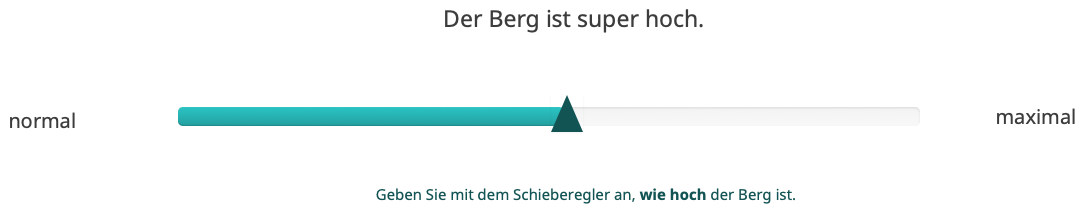
\includegraphics[width=\textwidth]{Skala1_2}
  \caption[Darstellung der in Experiment 2a verwendeten Bewertungsskala zu Skalarität] {Darstellung der in Experiment 2a verwendeten Bewertungsskala.}  
  \label{Bewertungsskala}
\end{figure}


\noindent Wie in {Abbildung \ref{Bewertungsskala}} zu sehen ist, unterschied sich die Skala in ihrer Gestaltung nicht von den in Kapitel \ref{Experiment0} beschriebenen Skalen zu Experiment 1: Während sie vor dem Betätigen des Schiebereglers farblos war, färbte sie sich mit dem Betätigen vom Nullpunkt bis zum gewählten Punkt hin ein, um den Versuchspersonen die zugeschriebene Intensität visuell zu verdeutlichen. Beschriftet war die Skala am linken Rand mit `normal' und am rechten Rand mit `maximal'. Lediglich im Hinblick auf die Aufgabenstellung unterschied sich diese Skala von den vorherigen: In Experiment 2a stand über der Skala der von den Versuchspersonen zu bewertende Satz, darunter die Aufgabenstellung, die im Wortlaut dem Itemsatz angepasst und in dem das jeweilige Adjektiv aus Gründen der Salienz fett hervorhoben war. Am Beispiel also: \textit{Geben Sie mit dem Schieberegler an, \textbf{wie hoch} der Berg ist}.
\noindent Um die Aufgabe zu erfüllen, war der Schieberegler durch Klicken oder Ziehen mit der Maus an diejenige Position zu bewegen, die der persönlichen Einschätzung nach am besten der Bedeutung des Satzes entspricht. Der gewählte Skalenwert steht dabei für den Ausprägungsgrad, den die Person mit der im Satz beschriebenen Eigenschaft, bspw. der Höhe des Bergs, {verbindet}.


Vor Beginn des Experiments wurden die Versuchspersonen in einer ausführlichen Instruktion über den Anlass, die Dauer und den Ablauf des Experiments sowie datenschutzrechtliche Aspekte informiert. Darüber hinaus wurden sie dazu aufgefordert, das Experiment an einem Endgerät mit physischer Tastatur durchzuführen. Durch diesen Hinweis sollte verhindert werden, dass die Skalen aufgrund unterschiedlicher Bildschirmgröße (Smartphone/Tablet vs. Notebook/Desktop-PC) nicht korrekt angezeigt oder nicht wie vorgesehen bedient werden können.\footnote{Zur Kontrolle wurde auch hier die Bildschirmgröße der Versuchspersonen erfasst.} Nach dem Einleitungstext erschienen zunächst die Übungssätze, die ebenso wie die Items einzeln abgefragt wurden und nach der Beantwortung unmittelbar und ohne weitere Erklärung in die für die Auswertung relevanten Testsätze übergingen.




\subsection{Versuchspersonen}\label{abs:Versuchspersonen2}
Die Personenstichprobe setzte sich aus 63 deutschen Muttersprachler:innen im Alter von 18 bis 40 Jahren zusammen, die keine Kenntnis über das Ziel der Untersuchung hatten. Diese wurden per \textit{Clickworker} rekrutiert und (bemessen an dem zu der Zeit gültigen deutschen Mindestlohn) mit je 1,70\,Euro entlohnt.
Auch dieses Experiment wurde mittels \textit{LimeSurvey} erstellt und von den Versuchspersonen individuell online bearbeitet. Die Dauer des Experiments betrug im Schnitt ca. zehn Minuten. Die Teilnahme erfolgte vollkommen anonym und ohne Erhebung personenbezogener Daten wie Alter, Geschlecht oder Herkunft.


Um zu gewährleisten, dass von jedem Intensivierer pro Liste sieben Datenpunkte und somit eine gleichmäßige Verteilung vorliegt, wurde die Teilnahme von 64 Versuchspersonen angestrebt. Nach dem Abschluss des Experiments kam es allerdings zu einer Komplikation vonseiten \textit{Clickworkers}, in deren Folge bloß Daten von 63 Personen zum Export zur Verfügung standen. Dadurch konnten letztlich fünf Listen mit Daten von je acht Versuchspersonen, zwei Listen mit Daten von je sieben Versuchspersonen sowie eine Liste mit Daten von neun Versuchspersonen exportiert werden, was in einem leichten Ungleichgewicht resultierte. Wie bereits beim vorangegangenen Experiment wurde dies aufgrund der Robustheit der gewählten statistischen Auswertungsmethode sowie dem häufig unvermeidbaren Ausschluss einzelner Versuchspersonen jedoch als nicht weiter problematisch erachtet.




\subsection{Ausschlusskriterien}
Auch für diese Untersuchung wurden im Vorfeld Ausschlusskriterien festgelegt. Wie schon in Experiment 1 beinhalteten diese vor allem die Kombination aus einer überschnellen Reaktionszeit und einem uniformen Antwortmuster, die ein bloßes Durchklicken der Person durch das Experiment nahelegt.


Von den 63 Versuchspersonen, deren Antworten exportiert werden konnten, gingen 61 in die Auswertung mit ein, wohingegen zwei Personen von der Analyse ausgeklammert wurden. Der Grund für den Ausschluss ebendieser lag darin, dass deren Ergebnis ein völlig einheitliches Muster ohne Variation in der Skalenbewertung aufwies. So positionierten sie den Schieberegler bei allen Intensivierern gleichermaßen am linken oder rechten Skalenrand, was ein Indiz dafür ist, dass sie die Aufgabe nicht aufmerksam bearbeitet, sondern sich lediglich durch das Experiment durchgeklickt haben. Diese Vermutung konnte durch eine Begutachtung der durchschnittlichen Reaktionszeit je Item erhärtet werden: Betrug die Reaktionszeit aller Versuchspersonen pro Item über das Experiment hinweg im Schnitt etwa 5,07 Sekunden ({\textit{SD} = 13,1}), lag die der ausgeschlossenen Personen deutlich darunter, nämlich bei 1,38 Sekunden ({\textit{SD} = 1,1}) und 1,91 Sekunden (\textit{SD} = 1,0). Dies erscheint kaum ausreichend, um einen gelesenen Satz korrekt zu verarbeiten und zu bewerten. Gemessen an den vergleichsweise niedrigen Reaktionszeiten und der uniformen Skaleneinschätzung war der Ausschluss dieser Personen legitim.
%1.38 Sekunden bei Proband 585636.4 bzw. bei 1.91 Sekunden bei Proband 




\subsection{Ergebnisse}\label{abs:Ergebnisse147}
Nachfolgend werden die Resultate von Experiment 2a vorgestellt, das auf die Ermittlung des Skalaritätsgrades von Intensivierern mit unterschiedlich wahrnehmbarer Intensität abzielte. Dieses diente der Überprüfung der Hypothese H6, nach der sich möglicherweise nicht nur zwischen, sondern auch innerhalb der Intensiviererklassen Unterschiede bzw. graduelle Abstufungen in Bezug auf den durch die Intensivierer ausgedrückten Intensitätsgrad zeigen, wie \citet[87]{Biedermann.1969} und \citet[408]{Breindl.2007} postulieren.


Wie beim vorangegangenen Experiment wird mit einer deskriptivstatistischen Auswertung begonnen, an die sich eine mittels R (Version 1.1.456, \citealt[]{R.2018}) und den Paketen \textit{lme4} (\citealt[]{Bates.2015}) und \textit{lmerTest} (\citealt[]{Kuznetsova.2017}) vorgenommene inferenzstatistische Auswertung anschließt. Die Visualisierung der Daten erfolgte zudem mit \textit{ggplot2} {(\citealt[]{Wickham.2016}}).

%Wie zuvor wurde letztere mittels R (Version 1.1.456, \citealt[]{R.2018}) und den Paketen \textit{lme4} (\citealt[]{Bates.2015}) und \textit{lmerTest} (\citealt[]{Kuznetsova.2017}) vorgenommen. Die Visualisierung der Daten erfolgte weiterhin mit \textit{ggplot2} (\citealt[]{Wickham.2016}). 


\subsubsection{Vergleich der Stufen}\label{abs:Deskriptivstatistik}


%Im Rahmen der deskriptivstatistischen Analyse werden zunächst die beiden Intensiviererklassen miteinander verglichen. Daran schließt sich eine Detailbetrachtung der einzelnen Intensivierer an, was einen besseren Überblick über die von den Versuchspersonen zugewiesenen Skalenwerte ermöglicht.



%\subsubsection{Vergleich der Intensiviererklassen} $~$ \\
\noindent Tabelle \ref{tab:Skalenwert1} bildet die gemittelten Skalenwerte und die Standardabweichungen für die beiden Intensiviererklassen, basierend auf 427 Datenpunkten pro Intensivierer, ab. An dieser Stelle werden die jeweils vier deskriptiven und expressiven Intensivierer zu einer Stufe zusammengefasst. Zusätzlich ist der Mittelwert für beide Stufen zusammen angegeben. 
%Die Anordnung erfolgt in alphabetischer Reihenfolge.

%
\begin{table}
%\setlength{\tabcolsep}{28.75pt}
\begin{tabularx}{.8\textwidth}{lrrrr}
\lsptoprule
Intensiviererklasse & Skalenwert &  (\textit{SD}) & Mittelwert &  \textit{SD}\\
\midrule
deskriptiv          & 58,18      &  (23,5)        & 60,43      & 23,8\\
expressiv           & 62,67      & (23,9)         & 60,43      & 23,8\\
\lspbottomrule
\end{tabularx}
\caption[Gemittelte Skalenwerte der Stufen bei Experiment 2a]{Gemittelte Skalenwerte und Standardabweichungen der Intensiviererklassen bei Experiment 2a -- Skalarität (in alphabetischer Reihenfolge).}
\label{tab:Skalenwert1}
\end{table}

\noindent Die Werte aus Tabelle \ref{tab:Skalenwert1} geben insgesamt Hinweise darauf, dass Sätze mit expressiven Intensivierern den Erwartungen gemäß von den Versuchspersonen hinsichtlich Skalarität auf der Skala um 4,50 Punkte höher eingestuft wurden als Sätze, die mit deskriptiven Intensivierern modifiziert wurden. Demnach wird der Skalaritätsgrad von expressiven Intensivierern bereits auf den ersten Blick als höher wahrgenommen als der von deskriptiven Intensivierern. Auch wenn der Unterschied zwischen den beiden Intensiviererklassen nicht übermäßig stark ausgeprägt ist, zeigt sich dennoch eine entsprechende Tendenz. Dieses Ergebnis deutet darauf hin, dass das Skalenrating als Untersuchungsmethode wie beabsichtigt funktioniert hat.


Die Tendenz zugunsten der expressiven Stufe ist ebenso anhand der in Abbildung \ref{Skalenwert2} dargestellten Boxplots zu erkennen.


\begin{figure}
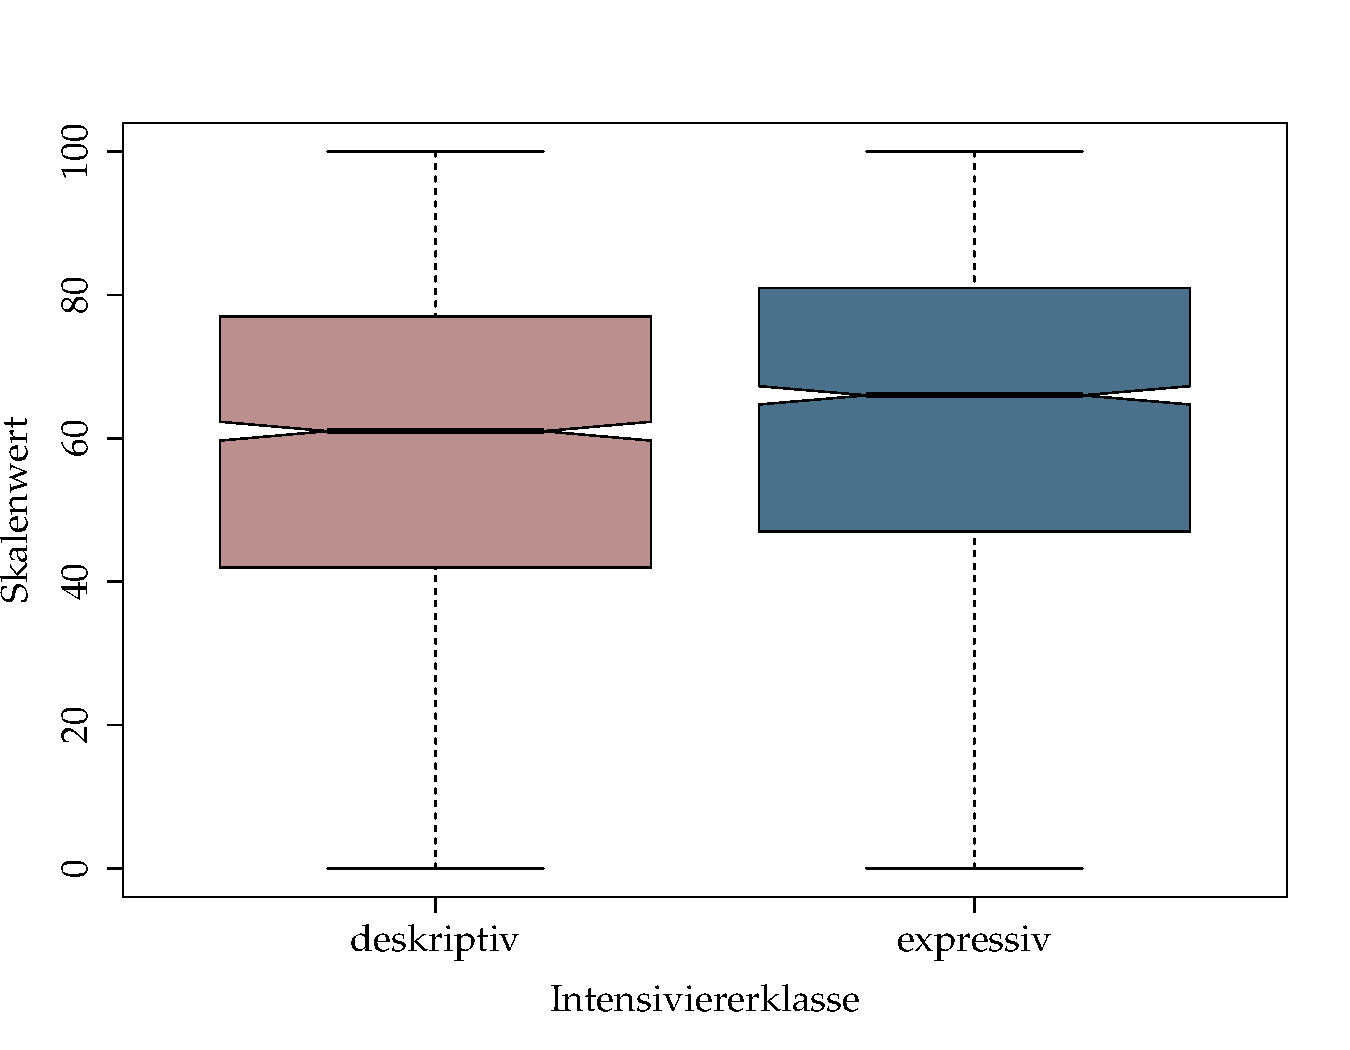
\includegraphics[width=1\textwidth]{Bedingung_E1_neu2}  
\caption[Gemittelte Skalenwerte der Stufen bei Experiment 2a] {Gemittelte Skalenwerte der Intensiviererklassen bei Experiment 2a -- Skalarität (x-Achse = Intensiviererklasse, y-Achse = Skalenwert).}
\label{Skalenwert2}
\end{figure}



\subsubsection{Regressionsanalyse zum Vergleich der Stufen}\label{LiGeMo1}


\noindent Nachfolgend werden die Ergebnisse der Regressionsanalyse zur Untersuchung von Skalarität vorgestellt. Das finale Modell wurde ausgehend vom vollen Modell per Rückwärtsselektion und Modellvergleich mithilfe der Funktion \textit{anova} in R schrittweise berechnet. Dazu wurde zunächst ein volles Regressionsmodell mit den Effekten aller unabhängigen Variablen und deren Zwei-Wege-Interaktionen berechnet, die möglicherweise Einfluss auf die abhängige Variable, d.\,h. den Skalaritätsgrad, hatten. Das volle Modell beinhaltete \textit{Fixed Effects} für den \textsc{Skalenwert} als metrische abhängige Variable sowie für die kategorialen Prädiktoren \textsc{Intensiviererklasse} und \textsc{Position} sowie deren Zwei-Wege-Interaktionen. In Experiment 2a steht die Variable \textsc{Skalenwert} für den Grad an Skalarität, den die Versuchspersonen mit der jeweiligen Intensiviererklasse bzw. dem jeweiligen Intensivierer assoziiert haben. Um einen potenziellen graduellen Effekt zwischen den Intensiviererklassen zu finden, wurde die nominale Variable \textsc{Intensiviererklasse} dummy-gecoded, wobei den Ausprägungsformen `Deskriptiv' und `Expressiv' die Werte $0$ und $1$ zugewiesen wurden. Diese wurden daraufhin miteinander verglichen. Außerdem wurden im vollen Modell versuchspersonenweise \textit{Random Intercepts} und \textit{Random Slopes} für die Variablen \textsc{Skalenwert}, \textsc{Intensiviererklasse} und \textsc{Position} miteingerechnet. Das bedeutet, dass auch mögliche Unterschiede zwischen den Versuchspersonen berücksichtigt wurden.\footnote{Da das volle Regressionsmodell unter Einbezug der Adjektive nicht konvergierte, konnten bei dieser Berechnung lediglich versuchspersonenweise \textit{Random Intercepts} und \textit{Random Slopes} miteingebunden werden.} Ausgehend vom vollen Modell wurden durch Rückwärtsselektion und Modellvergleich nach und nach all diejenigen Effekte getilgt, die den Modell-Fit nicht signifikant verbesserten. Das volle und finale Modell ist im Anhang \ref{RegX} zu sehen. Das finale Regressionsmodell enthält signifikante Haupteffekte für die Prädiktoren \textsc{Intensiviererklasse} und \textsc{Position}. Des Weiteren ist deren Zwei-Wege-Interaktion ebenfalls signifikant. Die berechneten Koeffizienten der Regressionsanalyse sind in {Tabelle \ref{LinReg01}} zusammengetragen.

%
\begin{table}
%\setlength{\tabcolsep}{8.75pt}
\begin{tabularx}{\textwidth}{Xrrrrr}
\lsptoprule
Prädiktor & \textit{Est.} & \textit{SE} & \textit{$\chi$$^{2}$} & \textit{p} & \\
\midrule

(Intercept) & 60,07 & 2,06 & 170,70 & < 0,001 & $\star$$\star$$\star$ \\
Intensiviererklasse & \textcolor{white}{-}4,47 & 1,47 & \textcolor{white}{-}\textcolor{white}{-}8,81 & < 0,01 & $\star$$\star$ \\
Position & -2,90 & 0,69 & \textcolor{white}{-}16,20 & < 0,001 & $\star$$\star$$\star$ \\
Intensiviererklasse\,:\,Position & -1,23 & 0,60 & \textcolor{white}{-}\textcolor{white}{-}4,17 & < 0,05 & \multicolumn{1}{r}{$\star$} \\
\lspbottomrule

\end{tabularx}
\caption[Finales Regressionsmodell von Experiment 2a (mit `Deskriptiv' als Referenzlevel)]{Finales Regressionsmodell von Experiment 2a -- Skalarität (mit `Deskriptiv' als Referenzlevel).}
\label{LinReg01}
\end{table}



%% IK: Wie verändert sich die Rating in Abhängigkeit von IK
%% Position numerisch
%% \textcolor{white}{-} So kann man einfach ein "weißes" Minus davorschreiben, das man nicht sieht, für ums unnernanner zu setzen


\noindent Wie der Übersicht in Tabelle \ref{LinReg01} zu entnehmen ist, haben zwei unabhängige Variablen sowie deren Zwei-Wege-Interaktion einen signifikanten Effekt auf den Skalenwert: \textsc{Intensiviererklasse} und \textsc{Position}. Demzufolge werden Sätze mit expressiven Intensivierern auf der Skala signifikant höher verortet als Sätze mit deskriptiven Intensivierern ($\chi$$^{2}$\,(1) = 8,81, \textit{p} < 0,01). Dieses Ergebnis steht im Einklang mit der in Experiment 1 untersuchten Hypothese H3 nach \citet[22]{Paradis.1997} und \citet[133]{Gutzmann.2019a} (vgl. Kapitel \ref{Experiment0}). Hinzu kommt ein signifikanter Positionseffekt: Je weiter fortgeschritten die Position eines Items im Experiment ist, desto niedriger wird es bezüglich Skalarität auf der Skala beurteilt {($\chi$$^{2}$\,(1) = 16,20,} {\textit{p} < 0,001}). Ferner ist die Interaktion zwischen beiden unabhängigen Variablen signifikant ($\chi$$^{2}$\,(1) = 4,17, \textit{p} < 0,05), was darauf hindeutet, dass sich die beiden Intensiviererklassen im Laufe des Experiments einander angenähert haben und der Unterschied zwischen deskriptiven und expressiven Intensivierern folglich kleiner geworden ist. Dies legt einen Gewöhnungseffekt nahe, der dem uniformen Untersuchungsdesign geschuldet sein kann. Somit besteht die Möglichkeit, dass sich die Versuchspersonen während des Experiments an die Intensivierer gewöhnt haben, weswegen sich der zu Beginn als stärker empfundene Unterschied zwischen den Intensiviererklassen sukzessive verringert hat.


Kurz gefasst belegen die Ergebnisse von {Experiment 2a} den in der Literatur vertretenen Unterschied zwischen deskriptiven und expressiven Intensivierern (vgl. \citealt[22]{Paradis.1997}; {\citealt[133]{Gutzmann.2019a}}). So wurden Sätze mit expressiven Intensivierern von den Versuchspersonen in der Tat mit einem höheren Grad an Skalarität assoziiert als Sätze, die mit einem deskriptiven Intensivierer präsentiert wurden. Der Umstand, dass sich der Unterschied zwischen den beiden Intensiviererklassen in aller Deutlichkeit zeigt, lässt außerdem den Schluss zu, dass das Skalenrating als Untersuchungsmethode wie intendiert funktioniert hat.



\subsubsection{Vergleich der Intensivierer}\label{LiGe}


\noindent Im nächsten Analyseschritt werden die gemittelten Skalenwerte der einzelnen Intensivierer betrachtet. Durch dieses Vorgehen können die untersuchten Ausdrücke in Bezug auf den ihnen von den Versuchspersonen zugewiesenen Skalaritätsgrad miteinander verglichen werden. Diese Werte finden sich inklusive Standardabweichungen in Tabelle \ref{Skalenwert3}. Die Anordnung der Intensivierer je Klasse erfolgt nach ansteigendem Skalenwert.

%
\begin{table}
%\setlength{\tabcolsep}{27pt}
\begin{tabularx}{.8\textwidth}{Xlrr}
\lsptoprule
Intensiviererklasse & Intensivierer  & Skalenwert &  \textit{SD}\\
\midrule
\rowcolor[gray]{.90}
deskriptiv & \textit{ziemlich} & 51,22 & 23,6\\
           & \textit{äußerst}  & 59,46 & 23,4\\
 \rowcolor[gray]{.90}
           & \textit{sehr}     & 59,69 & 23,3\\
           & \textit{überaus}  & 62,36 & 22,0\\
 \rowcolor[gray]{.90}
expressiv  & \textit{voll}     & 56,38 & 23,4\\
           & \textit{super}    & 63,15 & 22,2\\
 \rowcolor[gray]{.90}
           & \textit{sau}      & 63,87 & 24,4\\
           & \textit{mega}     & 67,27 & 24,4\\
\lspbottomrule

\end{tabularx}
\caption[Gemittelte Skalenwerte der einzelnen Intensivierer von Experiment 2a]{Gemittelte Skalenwerte und Standardabweichungen der einzelnen Intensivierer von Experiment 2a -- Skalarität (angeordnet nach ansteigendem Skalenwert).}
\label{Skalenwert3}
\end{table}

%
\noindent Aus den in Tabelle \ref{Skalenwert3} aufgeführten Werten lässt sich ableiten, dass den deskriptiven Intensivierern auch im Einzelnen betrachtet von den Versuchspersonen eine niedrigere Skalenposition zugesprochen wurde als den expressiven Intensivierern. So liegen beinahe alle deskriptiven Intensivierer auf der Skala durchschnittlich im Bereich zwischen 50 und 60 Punkten, wohingegen die expressiven Intensivierer vermehrt in einem Skalenbereich zwischen 60 und 70 Punkten angesiedelt sind. Nichtsdestotrotz scheint es in beiden Intensiviererklassen eine Ausnahme zu geben, nämlich \textit{überaus} aufseiten der deskriptiven Intensivierer und \textit{voll} aufseiten der expressiven Intensivierer. Das Ergebnis dieser Ausdrücke ist insofern überraschend, als dem deskriptiven Intensivierer ein verhältnismäßig hoher, dem expressiven Intensivierer hingegen ein verhältnismäßig niedriger Skalenwert zugewiesen wurde. Darüber hinaus manifestieren sich in beiden Intensiviererklassen tatsächlich graduelle Abstufungen, wie die Übersicht in Tabelle \ref{schwach0} nahelegt.


\begin{table}
\small
%\setlength{\tabcolsep}{8.25pt}
%\begin{tabular}{p{0.15\textwidth} p{0.1\textwidth} p{0.15\textwidth} p{0.1\textwidth} p{0.15\textwidth}}
\begin{tabularx}{\textwidth}{X@{} lrr lrr }
\lsptoprule
 &  \multicolumn{6}{c}{\textbf{Intensiviererklasse}}  \\
\cmidrule(lr){2-7}\cmidrule(lr){5-7}
& \multicolumn{3}{c}{{deskriptiv}} & \multicolumn{3}{c}{{expressiv}}  \\
\cmidrule(lr){2-4}\cmidrule(lr){5-7}
{Stärkegrad}  & Intensivierer & Skalenwert& \textit{SD}  & Intensivierer & Skalenwert& \textit{SD}   \\
\midrule
schwach & \textit{ziemlich} & 51,22& 23,6 & \textit{voll} & 56,38 & 23,4 \\
\multicolumn{1}{l}{mittel} & \textit{äußerst} & 59,46& 23,4  & \textit{super} & 63,15 & 22,2\\
 & \textit{sehr} & 59,69& 23,3 & \textit{sau} & 63,87& 24,4\\
stark & \textit{überaus} & 62,36& 22,0 & \textit{mega} & 67,27 & 24,4 \\
\lspbottomrule

\end{tabularx}
\caption[Klasseninterne Abstufungen bei Experiment 2a]{Klasseninterne Abstufungen bei Experiment 2a -- Skalarität (angeordnet nach ansteigendem Skalenwert).}
\label{schwach0}
\end{table}

\noindent Wie in Tabelle \ref{schwach0} zu beobachten ist, zeichnet sich innerhalb der deskriptiven Intensiviererklasse im Hinblick auf die von den Versuchspersonen wahrgenommene Skalarität folgendes dreistufiges Muster ab: {\textit{ziemlich} $\prec$ \textit{äußerst}|\textit{sehr} $\prec$ \textit{überaus}}. Ähnliches findet sich innerhalb der expressiven Intensiviererklasse: \textit{voll} $\prec$ \textit{super}|\textit{sau} $\prec$ \textit{mega}. Demnach wurde den deskriptiven Intensivierern \textit{äußerst} und \textit{sehr} von den Versuchspersonen ein nahezu identischer Skalenwert zugeschrieben ({$\Delta$ = ca. 0,23 Punkte}), genauso wie die expressiven Intensivierer \textit{super} und \textit{sau} auf der Skala ähnlich hoch positioniert wurden ($\Delta$ = ca. 0,72 Punkte). Diese Abstufungen lassen sich auch mithilfe des in Abbildung \ref{Bar1} dargestellten Säulendiagramms erkennen. Im Anhang \ref{Aja1} ist in Tabelle \ref{Adj0} außerdem eine Übersicht über die Ratings der Adjektive beigefügt. Darin ist zu sehen, dass deren Mittelwerte vergleichbar sind: Während das am niedrigsten eingestufte Adjektiv \textit{breit} auf der Skala durchschnittlich bei 58,06 Punkten angesiedelt ist, befindet sich das am höchsten verortete Adjektiv \textit{heiß} im Schnitt bei 64,80 Punkten. Die nur geringe Differenz von ca. 6,74 Punkten deutet auf ein Funktionieren der Methode hin. Andernfalls ließe sich spekulieren, dass der verzeichnete Unterschied zwischen den Intensiviererklassen ebenso den im Experiment verwendeten Adjektiven geschuldet sein könnte. Dies ist allerdings nicht {der Fall}.


%Wäre diese bspw. größer, so könnte der beobachtete Unterschied zwischen den Intensiviererklassen durch die verwendeten Adjektive geschuldet sein.



 
%
\begin{figure}
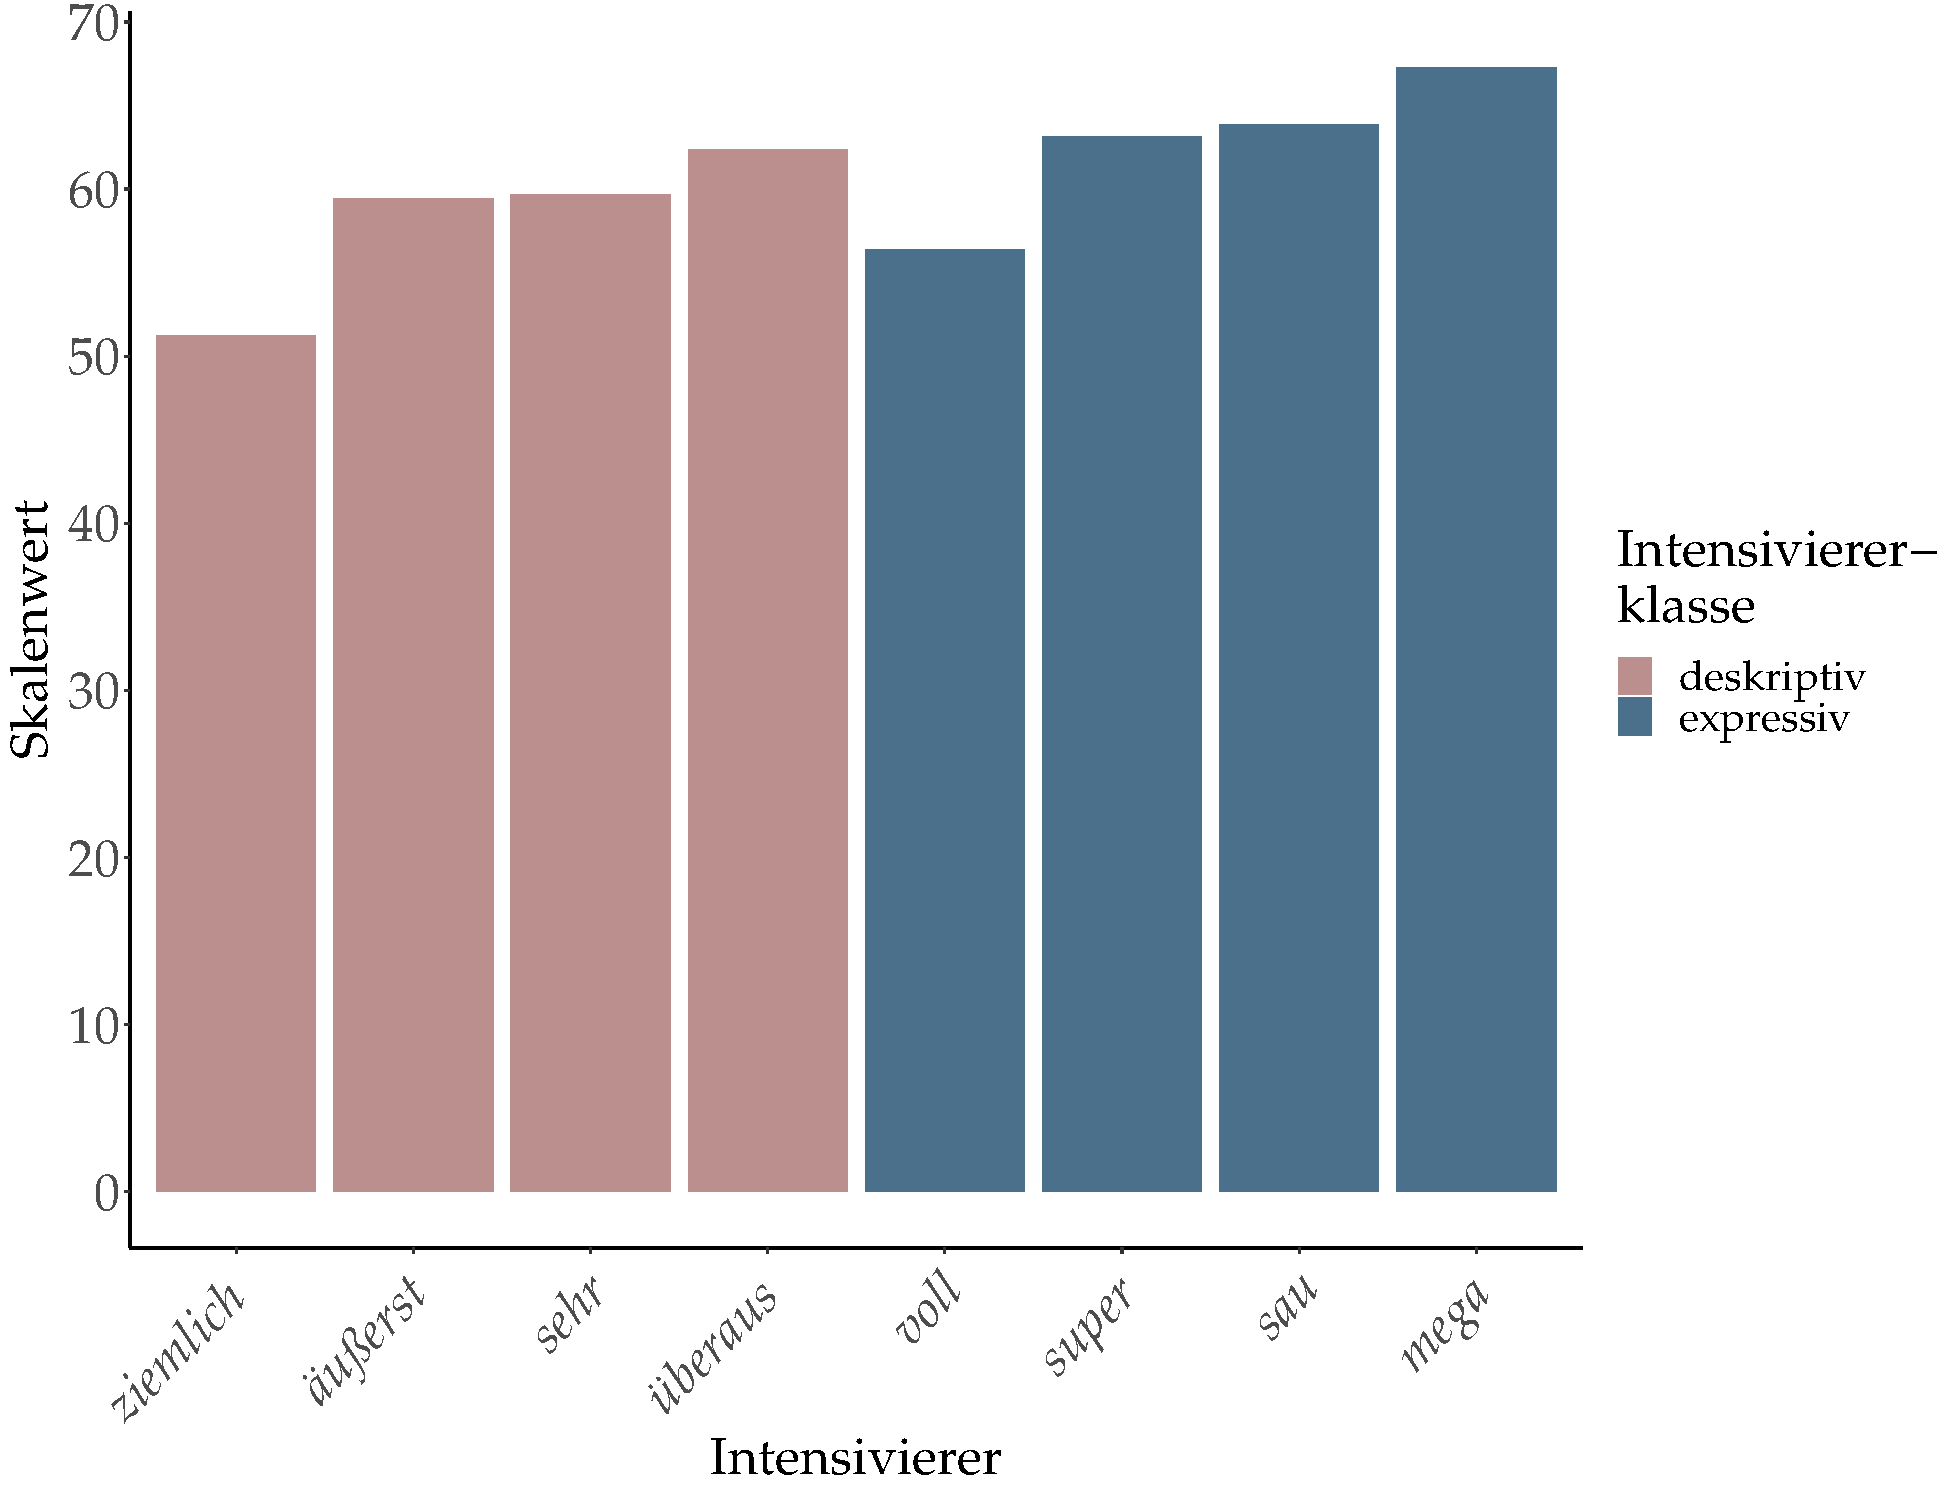
\includegraphics[width=1\textwidth]{Rplot_Bar_E1}
\caption[Säulendiagramm zu den einzelnen Intensivierern von Experiment 2a] {Säulendiagramm zu den einzelnen deskriptiven und expressiven Intensivierern von Experiment 2a -- Skalarität (x-Achse = Intensivierer, y-Achse = Skalenwert).}
\label{Bar1}
\end{figure}


\subsubsection{Paarweise Vergleiche der Intensivierer}\label{Paarweiser VerBie dengleich}


Um die beobachteten Unterschiede zwischen den einzelnen Ausdrücken auf Signifikanz hin zu überprüfen, wurden in einem weiteren Analyseschritt Paarvergleiche vorgenommen. Im Zuge dessen wurden die zugeschriebenen Skalenwerte der Intensivierer unter Zuhilfenahme des Inferenztests \textit{t}-Test gepaart miteinander verglichen. Exemplarisch am deskriptiven Intensivierer \textit{ziemlich} bedeutet die Gegenüberstellung, dass der Ausdruck erst mit \textit{äußerst} verglichen wurde, darauffolgend mit \textit{sehr}, mit \textit{überaus}, mit \textit{voll} etc. Durch dieses schrittweise Vorgehen konnte eine Matrix erstellt werden, in der das Ergebnis bzw. der Mittelwertunterschied des jeweils kontrastierten Intensiviererpaars festgehalten ist. Im Anschluss an die \textit{t}-Tests wurde eine Bonferroni-Korrektur angewandt, in deren Folge das Signifikanzniveau adjustiert wurde. Dieses Korrekturverfahren dient dazu, die bei multiplen Vergleichen mit gleicher Nullhypothese mögliche Alphafehler-Kumulierung zu vermeiden (vgl. {\citealt[249]{Wollschlaeger.2017}}; \citealt[176f.]{Winter.2020}). Beim Alphafehler wird die eigentlich korrekte Nullhypothese fälschlicherweise verworfen. Denn \glqq{}[m]it der Anzahl der Testwiederholungen steigt die Wahrscheinlichkeit (Gefahr), dass ein Unterschied als signifikant erscheint, auch wenn in Wirklichkeit keiner der Unterschiede signifikant ist.\grqq{} ({\citealt[186]{Backhaus.2018}}). Bei der Adjustierung des Signifikanzniveaus nach Bonferroni wurde der \textit{p}-Wert eines jeden gegenübergestellten Intensiviererpaars mit der Gesamtzahl der Testwiederholungen  multipliziert. Weil alle Intensivierer paarweise miteinander gekreuzt wurden, wurden insgesamt 28 Vergleiche durchgeführt: \textit{ziemlich} vs. \textit{äußerst}, \textit{ziemlich} vs. \textit{sehr}, \textit{ziemlich} vs. \textit{überaus}, \textit{ziemlich} vs. \textit{voll}, \textit{ziemlich} vs. \textit{super}, \textit{ziemlich} vs. \textit{sau}, \textit{ziemlich} vs. \textit{mega}, \textit{äußerst} vs. \textit{sehr}, \textit{äußerst} vs. \textit{überaus} usw. Infolge der Multiplikation mit der Anzahl der Testwiederholungen wird der jeweilige \textit{p}-Wert größer und ist gegebenenfalls weniger oder gar nicht mehr signifikant, wodurch dem Risiko des Alphafehlers {entgegengewirkt wird}.


Die aus den Berechnungen resultierende Matrix befindet sich in {Tabelle \ref{Matrix_1_neu}}.  In ihr sind die jeweiligen Testprüfgrößen der \textit{t}-Tests und die Bonferroni-korrigierten \textit{p}-Werte der einander gegenübergestellten Intensivierer gelistet. In der Tabelle erfolgen zunächst die Vergleiche der deskriptiven Intensivierer (in ansteigendem Skalenwert), hinterher die Vergleiche der expressiven Intensivierer (ebenfalls nach ansteigendem Skalenwert sortiert). Anzumerken ist, dass bei den darin gelisteten \textit{t}-Werten aus Gründen der Darstellbarkeit auf eine ausführliche Dokumentation mit eingeklammerter Angabe der Gesamtzahl der Freiheitsgrade (englisch: \textit{number of degrees of freedom}, hier und im Folgenden abgekürzt mit \textit{df}), die auf der Größe der jeweiligen Stichprobe basiert, verzichtet wird (\textit{t}\,(\textit{\textit{df}}) = \textelp{}). Bei den vorgenommenen Paarvergleichen entspricht der Freiheitsgrad dem Wert 3346. Aus diesem Grund gilt es zu beachten, dass die in der Tabelle jeweils angegebene verkürzte Form (bspw. \textit{t} = 6,84, {\textit{p} < 0,001}) streng genommen Folgendes meint: \textit{t}\,(3346) = \textelp{}. Angewandt auf das eingeklammerte Beispiel also {\textit{t}\,(3346) = 6,84,} {\textit{p} < 0,001}). Die Formel der Paarvergleiche findet sich außerdem im Anhang \ref{RegX}.



%\cellcolor[gray]{0.90}
%\cellcolor[gray]{0.75}
%\cellcolor[gray]{0.59}


%
\begin{sidewaystable}

%\setlength{\tabcolsep}{8pt}
\begin{tabularx}{\textwidth}{l@{~~}QQQQQQ@{}Q@{}Q@{}}
\lsptoprule
Intensivierer & \textit{ziemlich} & \textit{äußerst} & \textit{sehr} & \textit{überaus} & \textit{voll} & \textit{super} & \textit{sau} & \textit{mega} \\
\midrule

\multirow{3}{*}{\textit{ziemlich}} &  & \cellcolor[gray]{0.59}\textit{t} = 6,84, & \cellcolor[gray]{0.59} \textit{t} = 6,93, & \cellcolor[gray]{0.59} \textit{t} = 8,98, & \cellcolor[gray]{0.59} \textit{t} = 4,30,  & \cellcolor[gray]{0.59} \textit{t} = 9,64, & \cellcolor[gray]{0.59} \textit{t} = 10,39, & \cellcolor[gray]{0.59} \textit{t} = 12,82,  \\ 
& \hfil \ding{55} & \cellcolor[gray]{0.59}\textit{p} < 0,001  & \cellcolor[gray]{0.59}\textit{p} < 0,001   & \cellcolor[gray]{0.59}\textit{p} < 0,001   &   \cellcolor[gray]{0.59}\textit{p} < 0,001   &  \cellcolor[gray]{0.59}\textit{p} < 0,001  & \cellcolor[gray]{0.59}\textit{p} < 0,001  &  \cellcolor[gray]{0.59}\textit{p} < 0,001   \\ 
 &  & \cellcolor[gray]{0.59} $\star$$\star$$\star$ & \cellcolor[gray]{0.59} $\star$$\star$$\star$ & \cellcolor[gray]{0.59} $\star$$\star$$\star$  & \cellcolor[gray]{0.59} $\star$$\star$$\star$ & \cellcolor[gray]{0.59} $\star$$\star$$\star$ & \cellcolor[gray]{0.59} $\star$$\star$$\star$ &  \cellcolor[gray]{0.59} $\star$$\star$$\star$ \\ 
  
\multirow{3}{*}{\textit{äußerst}} & \cellcolor[gray]{0.59} \textit{t} = -6,84, &  & \textit{t} = 0,09, &  \textit{t} = 2,14, &  \textit{t} = -2,55,  &  \textit{t} = 2,80, & \cellcolor[gray]{0.90} \textit{t} = 3,55, &  \cellcolor[gray]{0.59} \textit{t} = 5,99,  \\ 
& \cellcolor[gray]{0.59} \textit{p} < 0,001 & \hfil \ding{55} & \textit{p} > 0,05   &  \textit{p} > 0,05 &   \textit{p} > 0,05   &  \textit{p} > 0,05  & \cellcolor[gray]{0.90} \textit{p} < 0,05   & \cellcolor[gray]{0.59} \textit{p} < 0,001    \\ 
& \cellcolor[gray]{0.59} $\star$$\star$$\star$  &  &  &    &  &  & \cellcolor[gray]{0.90} $\star$ &  \cellcolor[gray]{0.59} $\star$$\star$$\star$ \\ 

\multirow{3}{*}{\textit{sehr}} & \cellcolor[gray]{0.59} \textit{t} = -6,93, & \textit{t} = -0,09, &  &  \textit{t} = 2,06, &  \textit{t} = -2,64,  &  \textit{t} = 2,72, & \cellcolor[gray]{0.90} \textit{t} = 3,47, & \cellcolor[gray]{0.59} \textit{t} = 5,91,  \\ 
& \cellcolor[gray]{0.59}\textit{p} < 0,001  & \textit{p} > 0,05  & \hfil \ding{55}  &  \textit{p} > 0,05  &   \textit{p} > 0,05   & \textit{p} > 0,05  & \cellcolor[gray]{0.90} \textit{p} < 0,05    & \cellcolor[gray]{0.59}\textit{p} < 0,001   \\ 
 & \cellcolor[gray]{0.59} $\star$$\star$$\star$ & &  &    &  &  & \cellcolor[gray]{0.90} $\star$ &  \cellcolor[gray]{0.59} $\star$$\star$$\star$  \\ 

\multirow{3}{*}{\textit{überaus}} & \cellcolor[gray]{0.59} \textit{t} = -8,98, & \textit{t} = -2,14, & \textit{t} = -2,06, &   & \cellcolor[gray]{0.59}  \textit{t} = -4,69,  &  \textit{t} = 0,66, & \textit{t} = 1,42, & \cellcolor[gray]{0.75} \textit{t} = 3,85,  \\ 
& \cellcolor[gray]{0.59}\textit{p} < 0,001 & \textit{p} > 0,05  & \textit{p} > 0,05  &  \hfil \ding{55}  &   \cellcolor[gray]{0.59}\textit{p} < 0,001  &  \textit{p} > 0,05 & \textit{p} > 0,05  & \cellcolor[gray]{0.75}\textit{p} < 0,01   \\ 
 & \cellcolor[gray]{0.59} $\star$$\star$$\star$ &  &  &   & \cellcolor[gray]{0.59} $\star$$\star$$\star$  &  & &  \cellcolor[gray]{0.75} $\star$$\star$ \\ 

\multirow{3}{*}{\textit{voll}} & \cellcolor[gray]{0.59} \textit{t} = -4,30, & \textit{t} = 2,55, & \textit{t} = 2,64, &  \cellcolor[gray]{0.59} \textit{t} = 4,69, &    &  \cellcolor[gray]{0.59} \textit{t} = 5,36, &  \cellcolor[gray]{0.59}  \textit{t} = 6,11, & \cellcolor[gray]{0.59}  \textit{t} = 8,55,  \\ 
& \cellcolor[gray]{0.59}\textit{p} < 0,001 & \textit{p} > 0,05  & \textit{p} > 0,05  &  \cellcolor[gray]{0.59}\textit{p} < 0,001 &   \hfil \ding{55}  &  \cellcolor[gray]{0.59}\textit{p} < 0,001  & \cellcolor[gray]{0.59}\textit{p} < 0,001   & \cellcolor[gray]{0.59} \textit{p} < 0,001    \\ 
 & \cellcolor[gray]{0.59} $\star$$\star$$\star$ &  &  &  \cellcolor[gray]{0.59} $\star$$\star$$\star$  &  & \cellcolor[gray]{0.59} $\star$$\star$$\star$ &\cellcolor[gray]{0.59} $\star$$\star$$\star$ & \cellcolor[gray]{0.59} $\star$$\star$$\star$  \\ 

\multirow{3}{*}{\textit{super}} & \cellcolor[gray]{0.59} \textit{t} = -9,64, & \textit{t} = -2,80, & \textit{t} = -2,72, &  \textit{t} = -0,66, & \cellcolor[gray]{0.59}  \textit{t} = -5,36,  &   & \textit{t} = 0,76, & \cellcolor[gray]{0.90} \textit{t} = 3,19,  \\ 
& \cellcolor[gray]{0.59} \textit{p} < 0,001 & \textit{p} > 0,05 & \textit{p} > 0,05   & \textit{p} > 0,05  &   \cellcolor[gray]{0.59} \textit{p} < 0,001   &  \hfil \ding{55}  & \textit{p} > 0,05   & \cellcolor[gray]{0.90} \textit{p} < 0,05    \\ 
 & \cellcolor[gray]{0.59} $\star$$\star$$\star$ &  &  &    & \cellcolor[gray]{0.59} $\star$$\star$$\star$ &  & &    \cellcolor[gray]{0.90} $\star$\\ 
 
\multirow{3}{*}{\textit{sau}} & \cellcolor[gray]{0.59} \textit{t} = -10,39, & \cellcolor[gray]{0.90} \textit{t} = -3,55, & \cellcolor[gray]{0.90} \textit{t} = -3,47, &  \textit{t} = -1,42, &  \cellcolor[gray]{0.59} \textit{t} = -6,11,  &  \textit{t} = -0,76, &  & \textit{t} = 2,43,  \\ 
& \cellcolor[gray]{0.59}\textit{p} < 0,001  &  \cellcolor[gray]{0.90} \textit{p} < 0,05  & \cellcolor[gray]{0.90} \textit{p} < 0,05  &  \textit{p} > 0,05  &  \cellcolor[gray]{0.59}\textit{p} < 0,001   &  \textit{p} > 0,05   & \hfil \ding{55}  & \textit{p} > 0,05   \\ 
 & \cellcolor[gray]{0.59} $\star$$\star$$\star$  & \cellcolor[gray]{0.90} $\star$ & \cellcolor[gray]{0.90} $\star$ &   & \cellcolor[gray]{0.59} $\star$$\star$$\star$ &  & &   \\ 

\multirow{3}{*}{\textit{mega}} & \cellcolor[gray]{0.59} \textit{t} = -12,82, &  \cellcolor[gray]{0.59} \textit{t} = -5,99, & \cellcolor[gray]{0.59}  \textit{t} = -5,91, &  \cellcolor[gray]{0.75} \textit{t} = -3,85, &  \cellcolor[gray]{0.59} \textit{t} = -8,55,  &  \cellcolor[gray]{0.90} \textit{t} = -3,19, & \textit{t} = -2,43, &  \\ 
& \cellcolor[gray]{0.59}\textit{p} < 0,001  & \cellcolor[gray]{0.59}\textit{p} < 0,001  & \cellcolor[gray]{0.59}\textit{p} < 0,001   &  \cellcolor[gray]{0.75}\textit{p} < 0,01  &   \cellcolor[gray]{0.59}\textit{p} < 0,001   &  \cellcolor[gray]{0.90} \textit{p} < 0,05   & \textit{p} > 0,05  &  \hfil \ding{55}  \\ 
 & \cellcolor[gray]{0.59} $\star$$\star$$\star$  & \cellcolor[gray]{0.59} $\star$$\star$$\star$ & \cellcolor[gray]{0.59} $\star$$\star$$\star$  &  \cellcolor[gray]{0.75} $\star$$\star$ & \cellcolor[gray]{0.59} $\star$$\star$$\star$  &  \cellcolor[gray]{0.90} $\star$ & &   \\
\lspbottomrule
\end{tabularx}
\caption[Ergebnisse der Paarvergleiche der einzelnen Intensivierer von Experiment 2a]{Ergebnisse der Paarvergleiche der einzelnen Intensivierer bei Experiment 2a -- Skalarität (nach Bonferroni-Korrektur; angeordnet nach ansteigendem Skalenwert).}
\label{Matrix_1_neu}
\end{sidewaystable}





 Wie Tabelle \ref{Matrix_1_neu} zu entnehmen ist, führten die Paarvergleiche zu einigen diskutablen Feststellungen, die anschließend kurz beschrieben werden. Für einen besseren Überblick werden bloß diejenigen Ergebnisse aufgeführt, die signifikant sind, während die restlichen an dieser Stelle außen vor gelassen werden.\footnote{Der signifikante \textit{p}-Wert wird bloß bei der ersten Erwähnung eines miteinander verglichenen Intensiviererpaars angegeben (bspw. \textit{ziemlich} vs. \textit{äußerst}), wohingegen er bei der Zweitnennung aus Gründen der Übersichtlichkeit außen vor gelassen wird (\textit{äußerst} vs. \textit{ziemlich}).} Da den deskriptiven Intensivierern von den Versuchspersonen in Bezug auf Skalarität die niedrigsten Skalenwerte zugewiesen wurden und sie in der Tabelle daher den Ausgangspunkt bilden, werden zunächst die Werte von \textit{ziemlich} betrachtet. Den Ergebnissen der Paarvergleiche zufolge unterscheidet sich \textit{ziemlich} gänzlich von den restlichen Intensivierern, sind bei diesem Ausdruck doch alle Kontraste gleichermaßen signifikant: \textit{äußerst} {(\textit{t}\,(3346) = 6,84,} {\textit{p} < 0,001),} \textit{sehr} {(\textit{t}\,(3346) = 6,93,} {\textit{p} < 0,001)}, \textit{überaus} {(\textit{t}\,(3346) = 8,98}, {\textit{p} < 0,001)}, \textit{voll} {(\textit{t}\,(3346) = 4,30,} \textit{p} < 0,001), \textit{super} ({\textit{t}\,(3346) = 9,64,} \textit{p} < 0,001), \textit{sau} {(\textit{t}\,(3346) = 10,39,} \textit{p} < 0,001) und \textit{mega} {(\textit{t}\,(3346) = 12,82}, {\textit{p} < 0,001)}. Als Nächstes werden die Ergebnisse von \textit{äußerst} inspiziert. Hier finden sich signifikante Unterschiede bei den Vergleichen mit \textit{ziemlich}, \textit{sau} ({\textit{t}\,(3346) = 3,55, \textit{p} < 0,05)} und \textit{mega} {(\textit{t}\,(3346) = 5,99}, {\textit{p} < 0,001}). Gleichsam zeigen sich bei \textit{sehr} signifikante Unterschiede bei den Kontrasten mit \textit{ziemlich}, \textit{sau} (\textit{t}\,(3346) = 3,47, {\textit{p} < 0,05}) und \textit{mega} ({\textit{t}\,(3346) = 5,91}, {\textit{p} < 0,001)}. Bei \textit{überaus} sind darüber hinaus die Vergleiche mit \textit{ziemlich}, \textit{voll} ({\textit{t}\,(3346) = -4,69}, {\textit{p} < 0,001}) und \textit{mega} ({\textit{t}\,(3346) = 3,85,} {\textit{p} < 0,01}) signifikant.


Daneben weisen auch die Vergleiche der expressiven Intensivierer auf signifikante Unterschiede hin. So treten bei \textit{voll} signifikante Unterschiede bei den Kontrasten mit \textit{ziemlich}, \textit{überaus}, \textit{super} (\textit{t}\,(3346) = 5,36, \textit{p} < 0,001), \textit{sau} (\textit{t}\,(3346) = 6,11, \textit{p} < 0,001) und \textit{mega} (\textit{t}\,(3346) = 8,55, \textit{p} < 0,001) auf. Demnach unterscheidet sich \textit{voll} zur Gänze von den restlichen expressiven Intensivierern. Der nächste expressive Intensivierer in der Reihe ist \textit{super}. Bei diesem Ausdruck sind die Vergleiche mit \textit{ziemlich}, \textit{voll} und \textit{mega} (\textit{t}\,(3346) = 3,19, {\textit{p} < 0,05)} signifikant. Wie schon erwähnt, unterscheidet sich \textit{sau} signifikant von \textit{ziemlich}, \textit{äußerst}, \textit{sehr} und \textit{voll}. Aufgrund dessen, dass die Werte des expressiven Intensivierers \textit{mega} der Natur der Matrix gemäß bereits beschrieben wurden, werden die Resultate lediglich kurz wiederholt: Bei \textit{mega} sind signifikante Unterschiede bei den Vergleichen mit \textit{ziemlich}, \textit{äußerst}, \textit{sehr}, \textit{überaus}, \textit{voll} und \textit{super} zu beobachten. Das bedeutet, dass sich \textit{mega} mit Ausnahme von \textit{sau} ebenfalls gänzlich von den restlichen Intensivierern unterscheidet.


Zusammengefasst demonstrieren die Ergebnisse der Vergleiche, dass sich vor allem drei Ausdrücke klar von den anderen abheben: der deskriptive Intensivierer \textit{ziemlich} sowie die beiden expressiven Intensivierer \textit{mega} und \textit{voll}. Unterscheidet sich ersterer von jedem einzelnen anderen Ausdruck, verhält sich \textit{mega} anders als sechs und \textit{voll} anders als fünf der restlichen Intensivierer. Diese Befunde werden im nächsten Abschnitt \ref{abs:Diskussion} ausführlich besprochen.





\subsection{Diskussion} \label{abs:Diskussion}
In diesem Abschnitt werden die Ergebnisse von Experiment 2a diskutiert und unter Berücksichtigung der eingangs formulierten {Hypothese H6} evaluiert. Diese geht auf \citet[87]{Biedermann.1969} und {\citet[408]{Breindl.2007}} zurück, die von intraklassischen Unterschieden ausgehen. In diesem Sinne ist anzunehmen, dass sich die Ausdrücke in Abhängigkeit des durch sie ausgedrückten Intensitätsgrades auf einer kontinuierlichen Skala anordnen lassen. Ferner ist möglich, dass die Expressivität der Ausdrücke deren Skalaritätsgrad beeinflusst und letzterer in der Folge als stärker wahrgenommen wird {\citep[vgl.][133]{Gutzmann.2019a}}. Weil dieses Experiment, das dazu diente, den Skalaritätsgrad von Intensivierern mit unterschiedlich wahrnehmbarer Intensität zu ermitteln, und das anschließend vorgestellte {Experiment 2b}, das den Grad an Sprechereinstellung erfragte, als Ganzes betrachtet werden müssen, werden zunächst keine finalen {Schlüsse gezogen}.


In Experiment 2a ging es für die Versuchspersonen darum, auf einer Skala von `normal' bis `maximal' die Merkmalsausprägung eines im Satz beschriebenen Gegenstands anzugeben. Die Fragestellung war im Wortlaut jeweils an den Itemsatz angepasst, bspw. \textit{Wie hoch ist der Berg?}


Als erstes Ergebnis kann festgehalten werden, dass sich die beiden Intensiviererklassen hinsichtlich des ihnen zugeschriebenen Skalaritätsgrades deutlich voneinander unterscheiden (vgl. Tabelle \ref{LinReg01}). So wurde die Skalarität von Sätzen mit expressiven Intensivierern als signifikant stärker eingeschätzt als die Skalarität von Sätzen mit deskriptiven Intensivierern. Wie schon in dem in {Kapitel \ref{Experiment0}} präsentierten Experiment 1 spricht dieser Befund klar für die Gültigkeit der grundlegenden Annahme eines wahrnehmbaren Unterschiedes in der Skalarität von deskriptiven und expressiven Intensivierern (vgl. die {Hypothese H3} nach {\citealt[22]{Paradis.1997}} und {\citealt[133]{Gutzmann.2019a}}). Den Ergebnissen der beiden Untersuchungen zufolge verschieben expressive Intensivierer den Ausprägungsgrad der bezeichneten Eigenschaft auf einer Skala also tatsächlich weiter nach rechts als deskriptive Intensivierer, was als weitere Evidenz für die Hypothese H3 herangezogen {werden kann}.


Da in diesem Experiment vor allem die intraklassischen Abstufungen im Fokus standen, wurden die Intensiviererklassen im nächsten Analyseschritt aufgeschlüsselt und ihre Mitglieder einzeln inspiziert. Dabei trat sowohl bei den deskriptiven als auch den expressiven Intensivierern eine dreiteilige Abstufung im Hinblick auf den mit den Ausdrücken verbundenen Skalaritätsgrad auf, die sich wie folgt äußert: \textit{ziemlich} $\prec$ \textit{äußerst}|\textit{sehr} $\prec$ \textit{überaus} sowie {\textit{voll} $\prec$ \textit{super}|\textit{sau} $\prec$ \textit{mega}}. Demzufolge gibt es nach dem Empfinden der Versuchspersonen Intensivierer, die sich in Bezug auf den durch sie ausgedrückten Skalaritätsgrad stark ähneln, nämlich \textit{äußerst} und \textit{sehr} aufseiten der deskriptiven Intensivierer und \textit{super} und \textit{sau} aufseiten der expressiven Intensivierer. Dass die angenommenen Unterschiede auftreten, erhärtet das Zutreffen der zu testenden Hypothese H6. Die Ergebnisse decken sich in Teilen auch mit der in diesem Kontext dargelegten Rangfolge. Wie eingangs erläutert, verbinden {\citet[87]{Biedermann.1969}} und {\citet[408]{Breindl.2007}} den deskriptiven Intensivierer \textit{ziemlich} mit einem eher gemäßigten Intensitätsgrad. Gleiches zeigt sich in diesem Experiment, schätzten  die Versuchspersonen dessen Skalaritätsgrad doch ebenso vergleichsweise niedrig ein. Den beiden Intensivierern \textit{sehr} und \textit{überaus} sprechen die Autor:innen einen gemäßigten bis hohen bzw. hohen Intensitätsgrad zu, wohingegen sie \textit{äußerst} mit einem extremen Intensitätsgrad assoziiert sehen. In diesem Punkt zeichnen sich bei den durch das Experiment gewonnenen Ergebnissen Unterschiede ab, wurde \textit{äußerst} nicht auf höchster Stufe, sondern zusammen mit \textit{sehr} in der Mitte der Skala positioniert. Am stärksten wahrgenommen haben die Versuchspersonen den Skalaritätsgrad bei \textit{überaus}. Dies ist insofern bemerkenswert, als sich beide Ausdrücke aus semantischer Sicht kaum voneinander unterscheiden. So handelt es sich sowohl bei \textit{äußerst} als auch bei \textit{überaus} um native Ausdrücke, die qua Semantik angeben, dass ein kontextuell determinierter Schwellenwert überschritten wird. Im Gegensatz zu den deskriptiven Intensivierern entsprechen die Ergebnisse der expressiven Intensivierer gänzlich der im Vorfeld getroffenen persönlichen Einschätzung. Bei dieser Klasse bestand die Erwartung, dass das dem Anschein nach abgenutzte \textit{voll} nicht mehr ausdrucksstark genug ist, um als übermäßig skalar empfunden zu werden (vgl. die Resultate zu {Experiment 1}). Diese Annahme hat sich wiederholt bestätigt. Obendrein wurde davon ausgegangen, dass \textit{super} mit einem gemäßigten Skalaritätsgrad einhergeht, während er bei \textit{sau} und \textit{mega} mutmaßlich als am höchsten eingeschätzt wird. Den Ergebnissen nach sind auch diese Vermutungen im Wesentlichen korrekt, spiegelt sich innerhalb dieser Intensiviererklasse doch ausnahmslos die zuvor erwartete Rangfolge wider.


Mit dem Ziel die beobachteten Unterschiede auf Signifikanz hin zu überprüfen, wurden die Intensivierer anschließend paarweise miteinander verglichen (vgl. {Tabelle \ref{Matrix_1_neu}}). Wie vor diesem Hintergrund erläutert, sind dabei vor allem die Ergebnisse des deskriptiven Intensivierers \textit{ziemlich} auffällig. Dieser zeigt signifikante Unterschiede bei den Kontrasten mit allen anderen untersuchten Intensivierern -- unabhängig von der Intensiviererklasse. Schaut man sich die gemittelten Skalenwerte der Intensivierer an (vgl. {Tabelle \ref{Skalenwert3}}), so fällt auf, dass dem Ausdruck von den Versuchspersonen der mit Abstand niedrigste Grad an Skalarität zugeschrieben wurde, was höchstwahrscheinlich durch dessen inhärente Semantik bedingt ist: Anders als die restlichen Intensivierer drückt \textit{ziemlich} semantisch kein Übermaß einer bestimmten Eigenschaft aus, sondern approximiert lediglich einen bestimmten Referenzpunkt. So gibt bspw. \citet[1610]{Pfeifer.1995} dessen Bedeutung als `in verhältnismäßig hohem, reichlichem Maße, annähernd, ungefähr' an. Wie von {\citet[87]{Biedermann.1969}} und \citet[408]{Breindl.2007} korrekterweise gemutmaßt, scheint \textit{ziemlich} daher in der Tat als bloß moderat skalierend wahrgenommen zu werden, was der Hauptgrund für die signifikante Abweichung von den restlichen im Experiment berücksichtigten Intensivierern sein kann.


Ein weiteres auffälliges und somit diskutables Ergebnis ist beim expressiven Intensivierer \textit{mega} auszumachen, der von den Versuchspersonen mit dem höchsten Skalaritätsgrad assoziiert wurde. Bei den Paarvergleichen zeigte sich, dass sich der Ausdruck neben allen deskriptiven Intensivierern auch von den niedrig eingeschätzten expressiven Intensivierern \textit{voll} und \textit{super} signifikant unterscheidet. Auf Grundlage der bisherigen Resultate dieser Untersuchung ist diese Beobachtung kaum überraschend. So deuteten zum einen auch die Befunde der in {Kapitel \ref{Korpus}} präsentierten Korpusanalyse auf die Neuheit und anhaltende Beliebtheit dieses Intensivierers hin. Zum anderen deckt sie sich mit dem Ergebnis, das im vorangegangenen Experiment bei {Aufgabe I} auftrat: Auch hier war \textit{mega} der von den Versuchspersonen bezüglich Skalarität am höchsten beurteilte Intensivierer. Diese Ergebnisse bieten in Summe Anhaltspunkte dafür, dass \textit{mega} grundsätzlich mit einem hohen Skalaritätsgrad in Verbindung gebracht wird. Interessanterweise stimmt dies mit {\citet[]{Calpestrati.2017}} überein, der in seiner Korpusanalyse zu einem ähnlichen Schluss kommt. Demnach hat \textit{mega} anscheinend auch ein halbes Jahrzehnt später nichts von seiner wahrnehmbaren Intensität {eingebüßt}.


Ebenso bemerkenswert ist das Ergebnis von \textit{voll}, dessen Skalaritätsgrad innerhalb der expressiven Intensiviererklasse von den Versuchspersonen mit Abstand am niedrigsten empfunden wurde. Aus diesem Grund unterscheidet sich der Ausdruck bei den paarweisen Vergleichen signifikant von allen expressiven Intensivierern, von dem am höchsten eingeschätzten deskriptiven Intensivierer \textit{überaus} sowie dem am niedrigsten eingeschätzten deskriptiven Intensivierer \textit{ziemlich}. Eine mögliche Erklärung hierfür bietet die Überlegung, dass sich \textit{voll} unterdessen pragmatisch abgeschliffen hat und deswegen prinzipiell als nicht mehr stark skalierend {wahrgenommen wird}.


Auch der hinsichtlich Skalarität am zweithöchsten evaluierte expressive Intensivierer \textit{sau} unterscheidet sich signifikant von vier der restlichen Ausdrücke: den vergleichsweise niedrig eingeschätzten deskriptiven Intensivierern \textit{ziemlich}, \textit{äußerst} und \textit{überaus} sowie dem am niedrigsten bewerteten expressiven Intensivierer \textit{voll}. Dass \textit{sau} mit einem dem Anschein nach hohen Skalaritätsgrad assoziiert zu werden scheint, ist eventuell dessen klar erkennbarer Semantik geschuldet, die in Kombination mit der damit verbundenen derben Konnotation zur hohen Gradeinschätzung beigetragen haben kann.


Bei den Paarvergleichen war weiterhin festzustellen, dass sich \textit{äußerst} und \textit{sehr} parallel verhalten, die aufgrund ihres als beinahe identisch wahrgenommenen Skalaritätsgrades signifikante Unterschiede bei drei der restlichen Ausdrücke zeigen: dem am niedrigsten verorteten deskriptiven Intensivierer \textit{ziemlich} sowie den beiden als hoch eingeschätzten expressiven Intensivierern \textit{sau} und \textit{mega}. Im Gegensatz dazu unterscheidet sich der expressive Intensivierer \textit{super} ebenso signifikant von drei der anderen Ausdrücke: dem deskriptiven Intensivierer \textit{ziemlich}, dem am niedrigsten bewerteten expressiven Intensivierer \textit{voll} sowie dem am höchsten bewerteten expressiven Intensivierer \textit{mega}. Daraus lässt sich schließen, dass \textit{super} und \textit{sau} trotz der nahezu identischen Skaleneinschätzung bei den Paarvergleichen nicht die gleichen signifikanten Unterschiede aufweisen.


Kurz gefasst liefern die Ergebnisse von Experiment 2a erste stichhaltige Hinweise auf die Gültigkeit der zu testenden Hypothese H6 nach \citet[87]{Biedermann.1969} und \citet[408]{Breindl.2007}, finden sich bei der Untersuchung von Skalarität doch die vermuteten klasseninternen Abstufungen. Dies deutet darauf hin, dass sich die Ausdrücke im Hinblick auf den durch sie ausgedrückten Skalaritätsgrad de facto wahrnehmbar voneinander unterscheiden. Nachfolgend wird das parallel aufgebaute {Experiment 2b} vorgestellt. Dieses wurde separat durchgeführt und zielte darauf ab, den durch die Intensivierer ausgedrückten Grad an Sprechereinstellung zu ermitteln.

%Dies dient der Überprüfung, ob die im Kontext von Skalarität beobachtete Rangfolge in gleicher Weise bei Expressivität zutreffend ist und ob die Merkmale Skalarität und Sprechereinstellung im Sinne von {\citet[133]{Gutzmann.2019a}} miteinander korrelieren.
%Dabei ist anzunehmen, dass die Expressivität der Ausdrücke, wie von \citet[133]{Gutzmann.2019a} behauptet, Einfluss auf deren Skalaritätsgrad hatte. So drückten die expressiven Intensivierer relativ zu den deskriptiven Intensivierern auf jeder Stufe einen höheren Grad an Skalarität aus. 

%In diesem Sinne waren bei beiden Intensiviererklassen graduelle Abstufungen in Bezug auf den mit den Ausdrücken einhergehenden Skalaritätsgrad auszumachen: schwach $\prec$ mittel $\prec$ stark. Demzufolge können deskriptive Intensivierer entweder schwach, mittel oder stark skalierend sein, ebenso wie auch die expressiven Intensivierer als schwach, mittel oder stark skalierend wahrgenommen werden können. Hierbei sind die Ausdrücke in Abhängigkeit ihrer Intensiviererklasse auf zwei unterschiedlichen Skalen nebeneinander geordnet, die nach dem bspw. von {\citet[87]{Biedermann.1969}} und {\citet[408]{Breindl.2007}} vermuteten Intensitätsgrad abgestuft sind. Diese Idee wird in Tabelle \ref{schwach} genauer vorgeführt. Die Anordnung der Intensiviererklassen erfolgt in ansteigendem Skalenwert.



%%
%\begin{table}[h]
%
%%\setlength{\tabcolsep}{8.25pt}
%%\begin{tabularx}{\textwidth}{p{0.15\textwidth} p{0.1\textwidth} p{0.15\textwidth} p{0.1\textwidth} p{0.15\textwidth}}
%\begin{tabularx}{.8\textwidth}{Xlclc}
%\lsptoprule
% & & \multicolumn{2}{c}{\textbf{Intensiviererklasse}}  \\ [0.5em]
%\multirow{2}{*}{Stärkegrad} & \multicolumn{2}{c}{\textsc{deskriptiv}} & \multicolumn{2}{c}{\textsc{expressiv}}  \\ 
% & Intensivierer & Skalenwert & Intensivierer & Skalenwert  \\ 
%  &  & (\textit{SD})  &  & (\textit{SD})  \\
%\midrule 
%\\
%schwach & \textit{ziemlich} & 51,22 & \textit{voll} & 56,38  \\
% & & (23,6) & & (23,4)  \\
%\multicolumn{1}{l}{mittel} & \textit{äußerst} & 59,46 & \textit{super} & 63,15 \\
%& & (23,4) &  & (22,2)\\
% & \textit{sehr} & 59,69 & \textit{sau} & 63,87\\
%  & & (23,3) & & (24,4)\\
%stark & \textit{überaus} & 62,36 & \textit{mega} & 67,27  \\
% & & (22,0) & & (24,4)  \\
%\end{tabularx}
%\caption[Klasseninterne graduelle Abstufungen bei Experiment 2a]{Klasseninterne graduelle Abstufungen bei Experiment 2a -- Skalarität (in ansteigendem Skalenwert).}
%\label{schwach}
%\end{table}









%Nachfolgend wird das parallel aufgebaute {Experiment 2b} vorgestellt. Dieses wurde separat durchgeführt und zielte darauf ab, den durch die Intensivierer ausgedrückten Grad an Sprechereinstellung zu ermitteln.
%%Dies dient der Überprüfung, ob die im Kontext von Skalarität beobachtete Rangfolge in gleicher Weise bei Expressivität zutreffend ist und ob die Merkmale Skalarität und Sprechereinstellung im Sinne von {\citet[133]{Gutzmann.2019a}} miteinander korrelieren.



%So lieferten die im Rahmen der Korpusuntersuchung ermittelten diachronen Häufigkeitsverteilungen Hinweise darauf, dass der Ausdruck schon in den Sechzigerjahren vermehrt in intensivierender Funktion verwendet wurde. Daher ist davon auszugehen, dass er sich in der gesprochenen Sprache noch früher etabliert hat, was offenbar abträglich für die mit ihm einhergehende Intensität war. Nichtsdestotrotz stellt sich an der Stelle die Frage, aus welchen Gründen dem im Korpus ähnlich frequenten \textit{sau} von den Versuchspersonen der zweithöchste Skalaritätsgrad zugeschrieben wurde. Diesbezüglich lässt sich spekulieren, dass dies dessen klar erkennbarer Semantik geschuldet war, die in Kombination mit der damit verbundenen derben Konnotation zum hohen Skalenwert beigetragen haben kann. Ob diese Vermutung der Realität entspricht, lässt sich allerdings nicht eindeutig beantworten, zumal der Skalaritätsgrad von \textit{sau} im vorherigen Experiment nur unwesentlich höher eingestuft wurde als der von \textit{voll}.


%Bei den paarweisen Vergleichen der deskriptiven Intensivierer war festzustellen, dass sich \textit{äußerst} und \textit{sehr} parallel verhielten, die aufgrund beinahe identischer Skalenwerte (\textit{äußerst} = 59,46 Punkte und \textit{sehr} = 59,69 Punkte) gleichermaßen signifikante Unterschiede bei den Kontrasten mit \textit{ziemlich}, \textit{mega} und \textit{sau} anzeigten. Die möglichen Gründe hierfür wurden oben im Kontext der dreiteiligen Abstufung der Intensiviererklassen erörtert. Vor diesem Hintergrund wurde erklärt, dass \textit{äußerst} mit 19\,723 absoluten Treffern im Korpus nahezu doppelt so häufig zu finden ist wie \textit{überaus}, das darin nur 10\,534 absolute Treffer aufweist. Der vergleichsweise niedrige Skalenwert von \textit{überaus} (62,36 Punkte) war vermutlich nicht semantisch bedingt, unterschied sich dieser Ausdruck dahingehend doch kaum von anderen deskriptiven Intensivierern wie z.\,B. \textit{äußerst}. Eine bessere Erklärung bietet dagegen die Gebrauchsfrequenz: Da \textit{überaus} erwiesenermaßen seltener verwendet wird als die anderen deskriptiven Intensivierer, wurde er von den Versuchspersonen mutmaßlich als markierter wahrgenommen und in der Folge als stärker skalierend beurteilt.


%Zusammengenommen deuteten auch die Ergebnisse der Paarvergleiche auf einen deutlichen Unterschied zwischen den Intensiviererklassen hin.




%Dabei zeigte sich, dass die mittleren Werte der deskriptiven Intensivierer auch im Detail überwiegend unter denen der expressiven Intensivierer lagen. Dennoch war auf beiden Seiten eine Ausnahme auszumachen, nämlich der deskriptive Intensivierer \textit{überaus} und der expressive Intensivierer \textit{voll}. So wurde \textit{überaus} deutlich über den restlichen deskriptiven Intensivierern, \textit{voll} dagegen deutlich unter den restlichen expressiven Intensivierern eingestuft. Ob und inwiefern es sich bei diesen Intensivierern um Ausreißer handelt, hängt im Wesentlichen davon ab, wie eng man die oben skizzierte Hypothese H3 fasst, sind diesbezüglich doch zwei Interpretationsweisen denkbar: eine starke und eine schwache Interpretation. Gemäß ersterer, bei der sich deskriptive und expressive Intensivierer auf der gleichen Skala befinden, ist anzunehmen, dass der schwächste expressive Intensivierer im Hinblick auf Skalarität grundsätzlich höher positioniert wird als der stärkste deskriptive Intensivierer: {deskriptive Intensivierer $\prec$ expressive Intensivierer}. Dementsprechend gibt es Abstufungen in den Stärkegraden, die unabhängig von der Intensiviererklasse sind. Entscheidend ist alleine, dass die expressiven Intensivierer eine höhere Position auf der Skala einnehmen als die deskriptiven Intensivierer.
%Nach dieser Interpretation würde es sich bei \textit{überaus} und \textit{voll} tatsächlich um Ausreißer handeln. 
%In dem Fall ergibt sich die Frage, wieso sich die beiden Intensivierer anders verhielten als die restlichen Klassenmitglieder. Im Kontext von \textit{überaus} bietet die Annahme, dass es als Intensivierer vergleichsweise seltener -- und möglicherweise zu selten -- ist, eine mögliche Erklärung für vergleichsweise hoch eingeschätzten Skalaritätsgrad. Um diese Annahme zu überprüfen, wurde das absolute Vorkommen der deskriptiven Intensivierer im Nachgang anhand des gleichen Korpus, das im Fokus der in Kapitel \ref{Korpus} vorgestellten Korpusuntersuchung stand, ermittelt. Dabei stellte sich heraus, dass \textit{überaus} mit 10\,523 absoluten Treffern die niedrigste Belegdichte der deskriptiven Intensiviererklasse aufweist.\footnote{Die Belegtreffer der restlichen deskriptiven Intensivierer sehen wie folgt aus: \textit{äußerst}: 19\,723 absolute Treffer, \textit{ziemlich}: 54\,379 absolute Treffer und \textit{sehr}: 165\,161 absolute Treffer.} Bei diesem Ausdruck kann die niedrigere Frequenz also dazu geführt haben, dass er von den Versuchspersonen als markierter wahrgenommen wurde als die restlichen deskriptiven Intensivierer, was sich letztlich in dem ihm zugesprochenen Skalaritätsgrad widergespiegelt hat. Der expressive Intensivierer \textit{voll} ist hingegen eventuell schlichtweg zu abgenutzt. So konnten im Zeitschriftenkorpus schon um 1960 herum erste Belege für sein vermehrtes Vorkommen gefunden werden, was zeigt, dass es \textit{voll} schon lange Zeit in intensivierender Funktion gibt. Auffällig ist, dass dieses Ergebnis dem Befund entspricht, der sich im vorangegangenen Experiment 1 bei Aufgabe I zeigte: Auch hier wurde \textit{voll} von den Versuchspersonen mit einem verhältnismäßig niedrigen Skalaritätsgrad assoziiert ({vgl. {Tabelle \ref{SkaWe2}}}). Dies erhärtet den Verdacht, dass das intensivierende \textit{voll} inzwischen verbraucht ist, weswegen ihm grundsätzlich eine niedrigere Skalenposition zugesprochen wird als anderen expressiven Intensivierern.


%Neben der starken Interpretationsart der Hypothese H3 ist allerdings auch eine gemäßigtere vorstellbar. Nach dieser gibt es bei beiden Intensiviererklassen graduelle Abstufungen in Bezug auf den mit den Ausdrücken einhergehenden Skalaritätsgrad: schwach $\prec$ mittel $\prec$ stark. Dieser Einteilung nach können deskriptive Intensivierer entweder schwach, mittel oder stark skalierend sein, ebenso wie auch die expressiven Intensivierer als schwach, mittel oder stark skalierend wahrgenommen werden können. Hierbei sind die Intensiviererklassen auf zwei unterschiedlichen Skalen nebeneinander geordnet, die nach der Stärke der Skalierung abgestuft sind. Dadurch, dass die Grenzen der Stärkegrade parallel verschiebbar sind und sich die Abstufungen nur innerhalb einer Klasse abzeichnen, gibt es anders als bei der soeben umrissenen starken Interpretation keine Ausreißer, sondern Überlappungen zwischen den Intensiviererklassen. Daher würde es sich bei \textit{überaus} und \textit{voll} um Überlappungen handeln, die auf das Verschieben von zwei parallelen Skalen zurückgehen. Diese Idee wird in Tabelle \ref{schwach} genauer vorgeführt. Die Anordnung der Intensiviererklassen erfolgt in ansteigendem Skalenwert.



%
%\begin{table}[h]
%
%%\setlength{\tabcolsep}{8.25pt}
%%\begin{tabular}{p{0.15\textwidth} p{0.1\textwidth} p{0.15\textwidth} p{0.1\textwidth} p{0.15\textwidth}}
%\begin{tabularx}{.8\textwidth}{Xlclc}
%\lsptoprule
% & & \multicolumn{2}{c}{\textbf{Intensiviererklasse}}  \\ [0.5em]
%\multirow{2}{*}{Stärkegrad} & \multicolumn{2}{c}{\textsc{deskriptiv}} & \multicolumn{2}{c}{\textsc{expressiv}}  \\ 
% & Intensivierer & Skalenwert & Intensivierer & Skalenwert  \\ 
%  &  & (\textit{SD})  &  & (\textit{SD})  \\
%\midrule 
%\\
%schwach & \textit{ziemlich} & 51,22 & \textit{voll} & 56,38  \\
% & & (23,6) & & (23,4)  \\
%\multicolumn{1}{l}{mittel} & \textit{äußerst} & 59,46 & \textit{super} & 63,15 \\
%& & (23,4) &  & (22,2)\\
% & \textit{sehr} & 59,69 & \textit{sau} & 63,87\\
%  & & (23,3) & & (24,4)\\
%stark & \textit{überaus} & 62,36 & \textit{mega} & 67,27  \\
% & & (22,0) & & (24,4)  \\
%\end{tabularx}
%\caption[Schwache Interpretationsart als Erklärung für die Ausreißer von Experiment 2a]{Schwache Interpretationsart als Erklärung für die potenziellen Ausreißer von Experiment 2a -- Skalarität (in ansteigendem Skalenwert).}
%\label{schwach}
%\end{table}

%Abgesehen von diesem Befund konnte ein weiteres Ergebnis beobachtet werden, das es zu diskutieren gilt. So  deutete sich nämlich sowohl innerhalb der deskriptiven als auch der expressiven Intensiviererklasse eine dreiteilige Abstufung im Hinblick auf den gemittelten Skalenwert an, die sich wie folgt ausdrückte: \textit{ziemlich} $\prec$ \textit{äußerst}|\textit{sehr} $\prec$ \textit{überaus} sowie {\textit{voll} $\prec$ \textit{super}|\textit{sau} $\prec$ \textit{mega}}. Somit schien es nach Einschätzung der Versuchspersonen Intensivierer zu geben, die sich in Bezug auf den durch sie ausgedrückten Skalaritätsgrad stark ähnelten, nämlich \textit{äußert} (59,46 Punkte) und {\textit{sehr} (59,69 Punkte}) aufseiten der deskriptiven Intensivierer ($\Delta$ = ca. 0,23 Punkte) und {\textit{super} (63,15 Punkte)} und \textit{sau} (63,87 Punkte) aufseiten der expressiven Intensivierer {($\Delta$ = ca. 0,72 Punkte)}. Semantisch könnten die beiden Intensiviererpaare nicht unterschiedlicher sein: So handelt es sich bei \textit{äußerst} bspw. um einen transparenten Ausdruck, dessen Ursprungslexem deutlich wahrnehmbar ist. Anders als bei \textit{sehr}: Wie in Abschnitt \ref{Intensivierertypen} erörtert, ist der lexikalische Ursprung von \textit{sehr} unterdessen vollkommen opak. Dessen ungeachtet ist anzunehmen, dass sich die beiden Ausdrücke hinsichtlich ihres Lexikalisierungsgrades nicht sonderlich stark voneinander unterscheiden: Während es sich bei letzterem um den klassischen Vertreter der deskriptiven Intensiviererklasse handelt, der sowohl im schriftlichen wie auch im mündlichen Sprachgebrauch entsprechend frequent ist, kann \textit{äußerst} jedoch als ebenso stark lexikalisiert betrachtet werden. Diese Vermutung lässt sich auf Grundlage der erhobenen Korpusfrequenzen belegen. Im Korpus ist \textit{äußerst} mit 19\,723 absoluten Treffern bspw. erheblich frequenter als \textit{überaus}, das darin lediglich 10\,534 absolute Treffer aufweist. Demnach ist es möglich, dass der Lexikalisierungsgrad von \textit{äußerst} im Hinblick auf Skalarität zu einer vergleichbaren Einschätzung geführt hat wie die von \textit{sehr}. Ähnlich verhält es sich bei \textit{super} und \textit{sau}. Deren vergleichbarer Skalenwert ist insofern überraschend, als beide Ausdrücke ebenfalls über kaum semantische Gemeinsamkeiten verfügen: So handelt es sich bei \textit{super} um einen aus dem Griechischen entlehnten Ausdruck, der \textit{qua} Semantik mit einer dimensionalen Größe einhergeht. Dieser war mit ingesamt 391,26 Treffern pro Million Textwörter der am häufigsten verwendete Intensivierer im Korpus. Dagegen ist \textit{sau} ein nativer Ausdruck, dessen Ursprung im Tierreich zu verorten ist und der möglicherweise aufgrund seiner heutigen derben Konnotation den Weg in die Intensiviererrolle gefunden hat \citep[vgl.][360]{Claudi.2006}. Dieser Ausdruck lässt sich im Korpus mit 60,41 Treffern pro Million Textwörter nachweisen. Was die beiden Ausdrücke trotz dieser Unterschiede allerdings miteinander gemein haben, ist ihr persistenter Gebrauch, wie sich anhand der in {Abbildung \ref{SyDia}} dargestellten Histogramme herausstellte: So fanden sich sowohl für \textit{super} als auch für \textit{sau} schon zu Beginn des Untersuchungszeitraums erste Korpustreffer, was darauf hindeutet, dass sich die Intensivierer in der gesprochenen Sprache frühzeitig etabliert haben. Dieser persistente Gebrauch hat gegebenenfalls dazu geführt, dass die beiden Ausdrücke in der Zwischenzeit mit einem ähnlichen Skalaritätsgrad assoziiert werden und von den Versuchspersonen in der Konsequenz auf der Skala vergleichbar hoch {eingestuft wurden}.











%\subsubsection{Regressionsanalyse} $~$ \\
%Das in Tabelle \ref{LinReg1} präsentierte lineare gemischte Modell zeigte, dass die Prädiktoren \textsc{Intensiviererklasse} und \textsc{Position} sowie deren Interaktion signifikanten Einfluss auf den Skalenwert hatten. Demzufolge wurden expressive Intensivierer in Übereinstimmung mit der Hypothese H4 auf der Skala signifikant höher positioniert als deskriptive Intensivierer. Hinzu kam ein signifikanter Positionseffekt: Je weiter fortgeschritten die Position eines Items im Experiment war, desto niedriger wurde es im Hinblick auf Skalarität auf der Skala beurteilt. Die ebenfalls signifikante Zwei-Wege-Interaktion zwischen den beiden Variablen bedeutete außerdem, dass sich die Intensiviererklassen mit fortschreitender Position einander angenähert und der Unterschied zwischen deskriptiven und expressiven Intensivierern folglich kleiner geworden ist. Dies legt einen Gewöhnungseffekt nahe, der dem uniformen Untersuchungsdesign geschuldet sein kann. Somit besteht die Möglichkeit, dass sich die Versuchspersonen im Laufe des Experiments an die Intensivierer gewöhnt haben, weswegen sich der zu Beginn als stärker empfundene Unterschied zwischen den Intensiviererklassen sukzessive verringert hat.  
%Zusammengefasst deuten die Ergebnisse des Regressionsmodells \textit{de facto} auf einen signifikanten Unterschied zwischen beiden Intensiviererklassen hin, der sich durch eine höhere Skalenposition der expressiven Intensivierer ausdrückt, was in Einklang mit der zu testenden Hypothese steht.



%-	Die Wahrscheinlichkeit, dass XY dem Zufall geschuldet ist, ist sehr klein, da die Korrelation hochsignifikant ist
%-	Außerdem finden wir bei XY eine starke Korrelation
%-	XY ist XY und dies ist nicht zufallsbedingt 
%-	Mit einem Mean von





%%%%%%%%%%%%%%%%%%%%%%%%%%%%%%%%%%%%%%%%%%%%%%%%%%%%%%%%%%%%%%%%%%%%%%%%%%%%%%%%%%%%%%%%%%%%%%%%%%%%%%%%%%%%%%%
%%%%%%%%%%%%%%%%%%%%%%%%%%%%%%%%%%%%% EXPERIMENT II %%%%%%%%%%%%%%%%%%%%%%%%%%%%%%%%%%%%%%%%%%%%%%%%%%%%%%%%%%%
%%%%%%%%%%%%%%%%%%%%%%%%%%%%%%%%%%%%%%%%%%%%%%%%%%%%%%%%%%%%%%%%%%%%%%%%%%%%%%%%%%%%%%%%%%%%%%%%%%%%%%%%%%%%%%%





\section{Experiment 2b -- Sprechereinstellung}\label{abs:Sprechereinstellung}
In diesem Teilkapitel steht das zweite Experiment im Fokus. Wie {Experiment 2a} wurde auch dieses aus der Intention heraus umgesetzt, die in Abschnitt \ref{abs:Hypothese und Forschungsaufbau} beschriebene Hypothese H6 auf ihre Korrektheit hin zu überprüfen. In diesem Kontext ist davon auszugehen, dass sich nicht nur zwischen, sondern auch innerhalb der Intensiviererklassen graduelle Abstufungen beobachten lassen, die auf die Semantik der Ausdrücke zurückzuführen sind. Im Vorfeld dieser Untersuchung wird erwartet, dass die expressiven Intensivierer jeder Stufe von den Versuchspersonen als stärker bewertend beurteilt werden als die deskriptiven Intensivierer. Dabei stellt sich zudem die Frage, ob die in Experiment 2a beobachteten Abstufungen in gleicher Weise bei Sprechereinstellung zutage treten, die Intensivierer also in Bezug auf dieses Merkmal eine ähnliche Rangfolge wie bei Skalarität aufweisen. Diesbezüglich ist im Sinne von \citet[133]{Gutzmann.2019a} denkbar, dass die Expressivität der Ausdrücke deren Skalaritätsgrad beeinflusst, letzterer infolge der Expressivität als stärker wahrgenommen wird und es einen korrelativen Zusammenhang zwischen beiden Merkmalen gibt.





\subsection{Untersuchungsgegenstand}\label{abs:Untersuchungsgegenstand2509}
Bei dem in Experiment 2b verwendeten Testmaterial handelte es sich um die gleichen Items wie in Experiment 2a, in denen feste Kombinationen aus verschiedenen Nomen (n = 56) und skalaren Adjektiven (n = 7) mit jeweils vier deskriptiven und expressiven Intensivierern gekreuzt wurden: \textit{äußerst}, \textit{sehr}, \textit{überaus} und \textit{ziemlich} (deskriptiv) sowie \textit{mega}, \textit{sau}, \textit{super} und \textit{voll} (expressiv). Durch den parallelen Untersuchungsaufbau konnte maximale Vergleichbarkeit gewährleistet und die Ergebnisse der beiden Experimente in Bezug auf eine mögliche Korrelation hin überprüft werden. Zur Erinnerung werden die in (\ref{itemse1}) beispielhaft gelisteten Items erneut aufgeführt:

\ea
\ea Die Pfütze ist äußerst groß.
\ex Der Flur ist sehr lang.
\ex Die Mauer ist überaus hoch.
\ex Das Gemälde ist ziemlich alt.
\ex Die Straße ist mega breit.
\ex Das Wasser ist sau heiß.
\ex Der Stamm ist super dick.
\ex Das Schiff ist voll groß.
\z
\z
Somit wurde auch in diesem Experiment eine unabhängige Variable mit 8 Stufen untersucht: 4 deskriptive und 4 expressive Intensivierer. Die Kombination aus Nomen und Adjektiv wurde erneut nicht variiert. Stattdessen rotierte jede feststehende Nomen-Adjektiv-Kombination (n = 7) im Experiment über die Intensivierer, wodurch für jeden Intensivierer gleich viele Datenpunkte gesammelt werden konnten. Wie zuvor wurden die abzufragenden Items nach dem lateinischen Quadrat auf acht Versuchspersonengruppen verteilt, sodass jede Person eine dieser acht Listen mit insgesamt 56 Testsätzen mit je 28 deskriptiven und expressiven Items zu evaluieren hatte. Auch am Randomisierungsverfahren änderte sich nichts: Wiederholt wurde die Abfolge der Items nach dem Adjektiv pseudorandomisiert, um zu verhindern, dass das gleiche Adjektiv im Experiment direkt hintereinander folgt, was sich gegebenenfalls unerwünscht auf die Skaleneinschätzung ausgewirkt hätte.


Als Ergänzung zu den für die Auswertung relevanten Items wurden die zuvor konstruierten Übungssätze in das Experiment miteinbezogen. Diese verfügten über die gleiche syntaktische Struktur wie die Items, wiesen jedoch andere Intensivierer, Nomen und Adjektive auf. Die Übungssätze dienten im Wesentlichen dazu, die Versuchspersonen mit der Aufgabe, der Skala und der Bedienung des Schiebereglers vertraut zu machen. Wie schon in Experiment 2a wurden auch in diesem Experiment keine Distraktoren verwendet, da sie für die Zielsetzung der Untersuchung als überflüssig erachtet wurden.





%Neben der neuen Aufgabenstellung, die im nächsten Abschnitt vorgestellt wird, wurden auch die vier Trainingssätze modifiziert. Wie zuvor dienten diese im Wesentlichen dazu, die Versuchspersonen mit der Aufgabe und der Bedienung des Schiebereglers vertraut zu machen.
%, ohne dies zu explizieren. 
%Die neuen Übungssätze waren wie folgt konzipiert:
%
%\ex. \label{Übung2}
%\a. Das Fenster ist recht groß.
%\b. Das Chili ist extrem scharf.
%\b. Die Rolltreppe ist ganz steil.
%\b. Der Kühlschrank ist übelst neu.



\subsection{Untersuchungsdurchführung}\label{abs:Untersuchungsdurchführung2541}
Erneut wurden den Versuchspersonen am Computer kurze und syntaktisch einfach konstruierte Kopulasätze präsentiert, in denen verschiedene Objekte beschrieben wurden, wie bspw. \textit{Der Berg ist äußerst hoch}. Daraufhin wurden sie dazu aufgefordert, mit einem Schieberegler auf einer kontinuierlichen Skala anzugeben, wie bewertend die jeweilige Aussage ist (vgl. {Experiment 2a}: Wo lässt sich das im Satz beschriebene Objekt im Vergleich zu einem normal ausgeprägten Objekt auf der Skala verorten?). Um den Grad der ausgedrückten Sprechereinstellung zu ermitteln, wurde in {Experiment 2b} also die Aufgabenanweisung an die neue Zielsetzung angepasst. Das bedeutet, dass sich der Wortlaut der Fragestellung sowohl von der in {Experiment 2a} untersuchten Skalarität als auch von der in {Experiment 1} in Aufgabe II erfragten Sprechereinstellung unterschied. Während der Grund für die unterschiedlichen Fragestellungen zwischen den {Experimenten 2a und 2b} auf das jeweils zu untersuchende Merkmal, d.\,h. Skalarität und Sprechereinstellung, zurückgeht, ist der Unterschied zwischen Experiment 2b und {Experiment 1 -- Aufgabe II} durch die zeitliche Abfolge der Experimente begründet. So wurde letzteres erst nach der in diesem Kapitel dargelegten Untersuchung durchgeführt und konnte in Bezug auf die Fragestellung optimiert werden. Abbildung \ref{Bewertungsskala2} illustriert die in Experiment 2b verwendete Skala.

%
\begin{figure}[h] 

  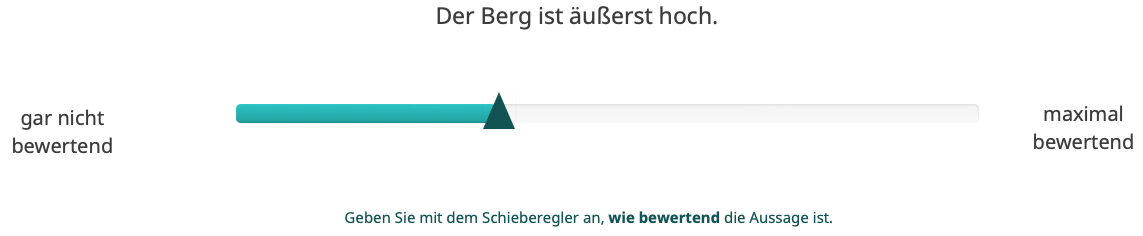
\includegraphics[width=1\textwidth]{Skala2_2}
 \caption[Darstellung der in Experiment 2b verwendeten Bewertungsskala zu Sprechereinstellung] {Darstellung der in Experiment 2b verwendeten Bewertungsskala.} 
  \label{Bewertungsskala2}
\end{figure}
%
%
%Da es in Experiment II jedoch nicht mehr um die Skalarität der Ausdrücke ging, sondern der Grad der Bewertung der Aussage erfragt werden sollte, wurde die Aufgabenformulierung an die neue Fragestellung angepasst. Der wesentliche Unterschied bei der zweiten Untersuchung bestand also darin, dass die Versuchspersonen auf einer Bewertungsskala einschätzen sollten, wie bewertend die jeweilige Aussage ist (vgl. Experiment I: Wo lässt sich das im Satz beschriebene Objekt im Vergleich zu einem vergleichbaren normalen Objekt auf der Skala verorten?). Der Leitgedanke einer solchen subjektiven Bewertung wurde den Versuchspersonen mithilfe von zwei Beispielsätzen folgendermaßen verdeutlicht:

%\begin{singlespace*}
%\begin{quotation} \glqq{}Im Folgenden werden Sie kurze Sätze lesen, wie zum Beispiel \textit{Das Auto steht im Hof} oder \textit{Ich habe die Klausur verkackt}. Ihre Aufgabe besteht darin, auf einer Skala einzuschätzen, wie bewertend die Aussage ist. Unter ‚bewertend‘ verstehen wir, dass der Sprecher den Sachverhalt subjektiv beurteilt. Während beide Beispielsätze einen Sachverhalt beschreiben (dass das Auto im Hof steht bzw. dass der Sprecher bei der Klausur schlecht abgeschnitten hat), ist der zweite Satz darüber hinaus bewertend, da der Sprecher zusätzlich seine Verärgerung über den Sachverhalt ausdrückt.\grqq{}\end{quotation}
%\end{singlespace*}

\noindent Wie Abbildung \ref{Bewertungsskala2} zeigt, war die Skala in Experiment 2b am linken Rand mit `gar nicht bewertend' und am rechten Rand mit `maximal bewertend' gelabelt (im Vergleich dazu `normal' bzw. `maximal' in {Experiment 2a}). Durch Betätigen des Reglers mit der Maus färbte sich die bis dahin farblose {Skala} vom Nullpunkt bis zum gewählten Punkt hin ein, wodurch die zugeschriebene Intensität für die Versuchspersonen visuell hervorgehoben wurde. Über der Skala befand sich der zu beurteilende Satz (bspw. \textit{Der Berg ist äußerst hoch}), darunter die Aufgabenstellung: \textit{Geben Sie mit dem {Schieberegler} an, \textbf{wie bewertend} die Aussage ist}. Um die Aufgabe zu erfüllen, war der Schieberegler durch Klicken oder Ziehen mit der Maus an diejenige Skalenposition zu bewegen, die der persönlichen Einschätzung nach den im Satz ausgedrückten Grad an Sprechereinstellung am besten wiedergibt. Kurz gefasst: Erfragte die Skala in Experiment 2a den Grad an Skalarität, ermittelte die in diesem Experiment verwendete Skala den Grad an {Sprechereinstellung}.


Auch dieses Mal wurden die Versuchspersonen in einem ausführlichen Einleitungstext über den Anlass, die Dauer und den Ablauf des Experiments inklusive datenschutzrechtlicher Aspekte informiert. Zudem wurden sie darum gebeten, das Experiment an einem Endgerät mit physischer Tastatur zu bearbeiten, wodurch verhindert werden sollte, dass die Skalen aufgrund unterschiedlicher Bildschirmgröße (Smartphone/Tablet vs. Notebook/Desktop-PC) nicht korrekt angezeigt oder nicht wie vorgesehen bedient werden können.\footnote{Wie schon in Experiment 2a wurde zur Kontrolle die Bildschirmgröße der Versuchspersonen erfasst.} Im Anschluss an die Instruktion startete das Experiment mit den Übungssätzen, die nach der Beantwortung nahtlos und ohne weitere Erklärung in die für die Auswertung bedeutsamen Items {übergingen}.



\subsection{Versuchspersonen}\label{abs:Probanden2}
Am Experiment haben 63 deutsche Muttersprachler:innen im Alter von 18 bis 40 Jahren teilgenommen, die über \textit{Clickworker} angeworben und (bemessen an dem zu der Zeit gültigen deutschen Mindestlohn) mit jeweils {1,70 Euro} {entlohnt} wurden. Die Versuchspersonen erhielten keine Informationen über das Ziel der Untersuchung. Wie zuvor wurde das Experiment mittels {\textit{LimeSurvey}} erstellt und von den Versuchspersonen individuell online durchgeführt. Die Durchführung war vollkommen anony, ohne dass personenbezogene Daten erhoben wurden. Die Dauer der Bearbeitung betrug im Schnitt etwa zehn Minuten.


Auch bei diesem Experiment wurde die Teilnahme von 64 Versuchspersonen angestrebt, um zu gewährleisten, dass von jedem Intensivierer sieben Datenpunkte und somit eine gleichmäßige Verteilung vorliegt. Erneut kam es nach Abschluss des Experiments zu einem Problem von \textit{Clickworker}, infolge dessen nur Daten von 63 Personen exportiert werden konnten. Dadurch lagen letztlich fünf Listen mit Daten von je acht Versuchspersonen, zwei Listen mit Daten von je sieben Versuchspersonen und eine Liste mit Daten von neun Versuchspersonen vor, die bei der Auswertung berücksichtigt wurden.



\subsection{Ausschlusskriterien}\label{abs:Auswertungskriterien2}
Von den 63 Versuchspersonen, deren Antworten exportiert wurden, flossen 62 in die Auswertung mit ein. Die Daten einer Versuchsperson wurden auf Basis von im Vorfeld der Untersuchung definierten Ausschlusskriterien von der Analyse ausgenommen, weil sie die Vermutung nahelegten, dass die Person die Aufgabe nicht aufmerksam bearbeitet, sondern sich lediglich durch das Experiment durchgeklickt hat. Dies äußerte sich in uniformen Angaben ohne Variation in der Skaleneinschätzung. Dieser Verdacht wurde durch eine Begutachtung der durchschnittlichen Reaktionszeit je Item bestätigt: Während die Reaktionszeit aller Versuchspersonen im Schnitt bei etwa 5,76 Sekunden lag {(\textit{SD} = 37,3)}, betrug die der ausgeklammerten Person dagegen bloß 1,38 Sekunden ({\textit{SD} = 0,9}). Die verhältnismäßig niedrige Reaktionszeit und das einheitliche Antwortmuster führten letztlich zu einem Ausschluss dieser Versuchsperson, sodass in der Auswertung bloß repräsentative Ergebnisse {berücksichtigt wurden}.




\subsection{Ergebnisse}\label{abs:Ergebnisse2576}
Nachfolgend werden die Ergebnisse von Experiment 2b präsentiert, das mit der Intention durchgeführt wurde, den Grad an Sprechereinstellung bei Intensivierern mit unterschiedlich wahrnehmbarer Intensität zu ermitteln. {Dadurch} wird die Gültigkeit der Hypothese H6 überprüft, nach der von klasseninternen Unterschieden in Bezug auf den durch die Intensivierer ausgedrückten Intensitätsgrad auszugehen ist, wie von {\citet[87]{Biedermann.1969}} und \citet[408]{Breindl.2007} angeführt wird. Ferner besteht im Sinne von {\citet[133]{Gutzmann.2019a}} die Möglichkeit, dass die Expressivität der Ausdrücke auf deren Skalaritätsgrad einwirkt und letzterer deswegen als stärker wahrgenommen wird. Auch diese Annahme wird getestet.


Begonnen wird mit einer deskriptivstatistischen Analyse, auf die eine inferenzstatistische Analyse folgt. Im Zuge dessen werden die Ergebnisse der beiden {Experimente 2a und 2b} ebenso auf eine mögliche Korrelation zwischen den Variablen \textsc{Skalarität} und \textsc{Sprechereinstellung} hin untersucht. Die inferenzstatistische Analyse wurde auch in diesem Experiment mithilfe von R (Version 1.1.456, \citealt[]{R.2018}) und den Paketen \textit{lme4} ({\citealt[]{Bates.2015}}) und \textit{lmerTest} (\citealt[]{Kuznetsova.2017}) vorgenommen. Die Visualisierung der Daten erfolgte darüber hinaus mit \textit{ggplot2} (\citealt[]{Wickham.2016}).


\subsubsection{Vergleich der Stufen}\label{abs:Deskriptivstatistik02}


%Wie zuvor werden zunächst die Intensiviererklassen einander gegenübergestellt, woraufhin eine genaue Begutachtung der einzelnen Intensivierer folgt.



%\subsubsection{Vergleich der Intensiviererklassen}\label{Intensiv2} $~$ \\
\noindent In Tabelle \ref{SkaWe_E2} sind die gemittelten Skalenwerte und Standardabweichungen für beide Intensiviererklassen, basierend auf 434 Datenpunkten pro Intensivierer, aufgeführt. An dieser Stelle werden die je vier deskriptiven und expressiven Intensivierer zu einer Stufe zusammengefasst. Auch hier ist als Ergänzung der Mittelwert für beide Stufen zusammen angegeben. 


%
\begin{table}
%\setlength{\tabcolsep}{28.75pt}
\begin{tabularx}{.8\textwidth}{Xrrrr}
\lsptoprule
Intensiviererklasse & Skalenwert &  \textit{SD} & Mittelwert &  \textit{SD}\\
\midrule
deskriptiv          & 49,15      &  27,8        & 54,79      &  28,7\\
expressiv           & 60,43      & 28,5         & 54,79      &  28,7\\
\lspbottomrule
\end{tabularx}
\caption[Gemittelte Skalenwerte der Stufen bei Experiment 2b]{Gemittelte Skalenwerte und Standardabweichungen der Intensiviererklassen bei Experiment 2b -- Sprechereinstellung (in alphabetischer Reihenfolge).}
\label{SkaWe_E2}
\end{table}


\noindent Der Übersicht in Tabelle \ref{SkaWe_E2} ist zu entnehmen, dass Sätzen mit expressiven Intensivierern von den Versuchspersonen ein tendenziell höherer Skalenwert zugeschrieben wurde als Sätzen mit deskriptiven Intensivierern {($\Delta$ = ca. 11,30 Punkte)}. Die gemittelten Skalenwerte der Intensiviererklassen unterscheiden sich bei der in Experiment 2b abgefragten Sprechereinstellung also wesentlich stärker voneinander als bei der in Experiment 2a untersuchten Skalarität. Der Wert von letzterer belief sich nämlich bloß auf 4,50 Punkte. Dies legt nahe, dass die Untersuchungsmethode funktioniert hat und die Einteilung der Ausdrücke in deskriptiv und expressiv insgesamt {passend war}.


Den markanten Unterschied zwischen den beiden Intensiviererklassen zeigen auch die in {Abbildung \ref{Box2}} dargestellten Boxplots.


\begin{figure}
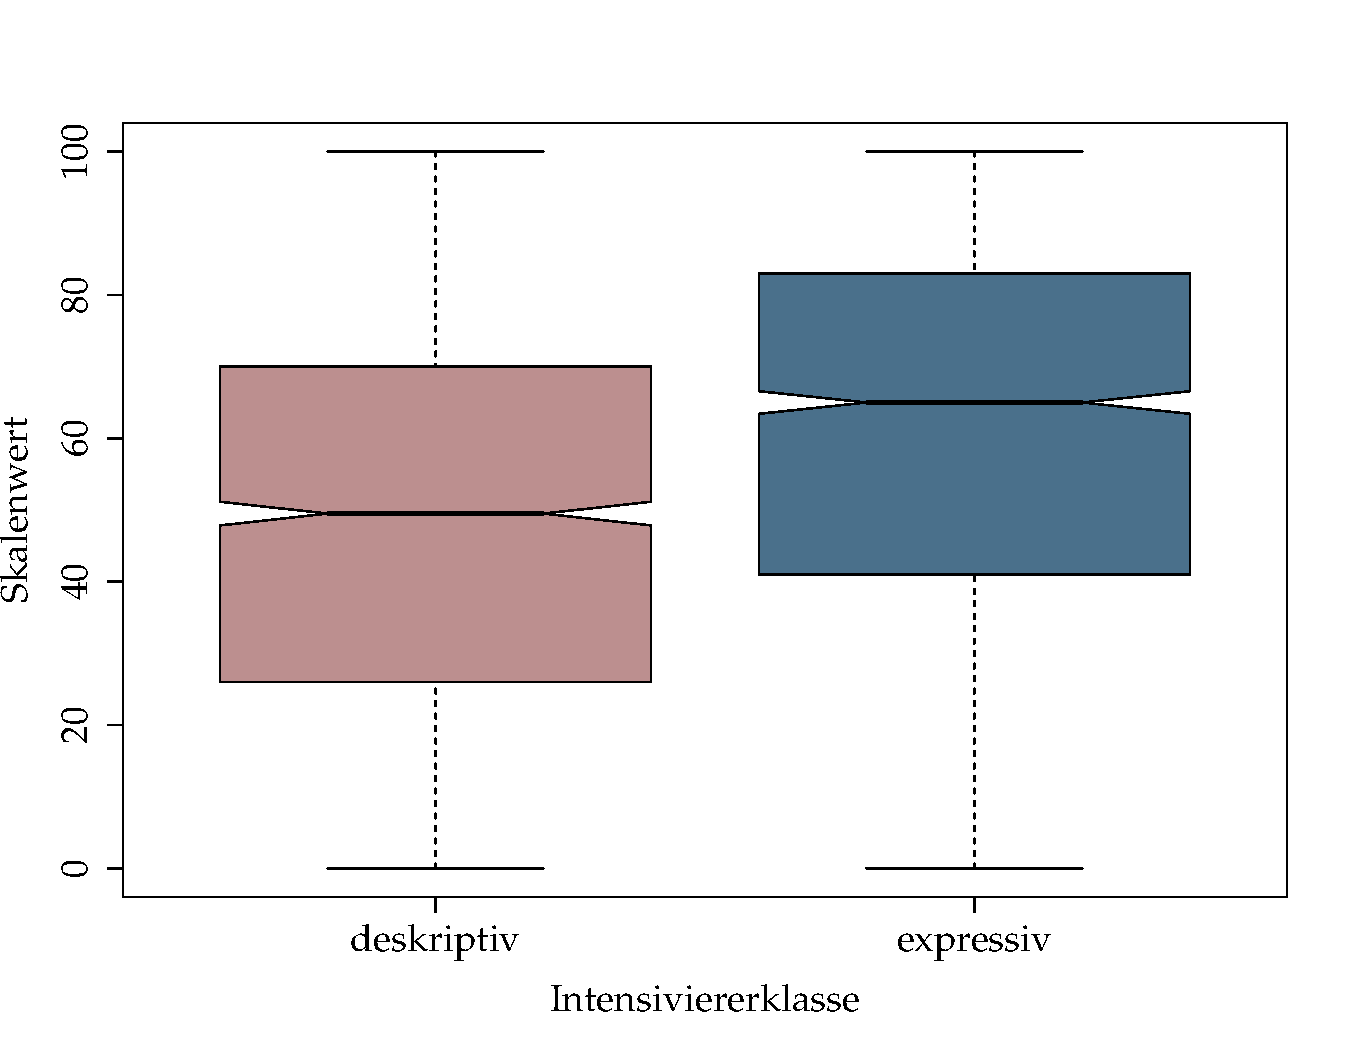
\includegraphics[width=1\textwidth]{Rplot_Box_E2}
\caption[Gemittelte Skalenwerte der Stufen bei Experiment 2b] {Gemittelte Skalenwerte der Intensiviererklassen bei {Experiment 2b --} Sprechereinstellung (x-Achse = Intensiviererklasse, y-Achse = Skalenwert).}
\label{Box2}
\end{figure}



\subsubsection{Regressionsanalyse zum Vergleich der Stufen}\label{LiGeMo02}
\largerpage

In diesem Abschnitt werden die Ergebnisse der Regressionsanalyse zur Untersuchung von Sprechereinstellung präsentiert. Wie das vorherige Modell wurde auch dieses durch Rückwärtsselektion und \textit{anova}-Modellvergleich in R berechnet. Wiederholt wurde zunächst ein volles Modell mit den Effekten aller unabhängigen Variablen und deren Zwei-Wege-Interaktionen berechnet, die sich möglicherweise auf die abhängige Variable ausgewirkt haben. Das volle Modell enthielt \textit{Fixed Effects} für den \textsc{Skalenwert} als metrische abhängige Variable sowie die kategorialen Prädiktoren \textsc{Intensiviererklasse} und \textsc{Position} sowie deren Zwei-Wege-Interaktionen. In {Experiment 2b} steht die Variable \textsc{Skalenwert} für den Grad an Sprechereinstellung, den die Versuchspersonen der jeweiligen Intensiviererklasse bzw. dem jeweiligen Intensivierer zugeschrieben haben. Um potenzielle Unterschiede zwischen den Intensiviererklassen zu finden, wurde die nominale Variable \textsc{Intensiviererklasse} dummy-gecoded. Dabei wurde `Deskriptiv' der Wert $0$ und `Expressiv' der Wert $1$ zugewiesen. Diese Ausprägungsformen wurden anschließend miteinander verglichen. Neben den \textit{Fixed Effects} wurden im vollen Modell versuchspersonenweise \textit{Random Intercepts} und \textit{Random Slopes} für die Variablen \textsc{Skalenwert}, \textsc{Intensiviererklasse} und \textsc{Position} miteinbezogen.\footnote{Da das volle Regressionsmodell unter Einbezug der Adjektive nicht konvergierte, konnten bei dieser Berechnung lediglich versuchspersonenweise \textit{Random Intercepts} und \textit{Random Slopes} miteingebunden werden.} Im Rahmen der Datenmodellierung wurden nach und nach all diejenigen Effekte getilgt, die den Modell-Fit nicht signifikant verbesserten und somit keinen Einfluss auf den Skalenwert hatten. Das volle und finale Modell ist im Anhang  \ref{Aja2} angegeben. Letzteres beinhaltet einen signifikanten Haupteffekt für den Prädiktor \textsc{Intensiviererklasse}. Die berechneten Koeffizienten der Regressionsanalyse befinden sich in {Tabelle \ref{LinReg2}}.

%
\begin{table}
%\setlength{\tabcolsep}{13pt}
%\begin{tabular}{p{0.425\textwidth} p{0.1\textwidth} p{0.1\textwidth} p{0.1\textwidth}p{0.1\textwidth} p{0.05\textwidth}}
\begin{tabularx}{.8\textwidth}{Xrrrrr}
\lsptoprule
Prädiktor & \textit{Est.} & \textit{SE} & \textit{$\chi$$^{2}$} & \textit{p} & \\
\midrule

(Intercept) & 49,02 & 2,68 & 39,31 & < 0,001 & $\star$$\star$$\star$\\
Intensiviererklasse & 11,02 & 2,70 & 14,51 & < 0,001 & $\star$$\star$$\star$\\
\lspbottomrule

\end{tabularx}
\caption[Finales Regressionsmodell von Experiment 2b (mit `Deskriptiv' als Referenzlevel)]{Finales Regressionsmodell von Experiment 2b -- Sprechereinstellung (mit `Deskriptiv' als Referenzlevel).}
\label{LinReg2}
\end{table}

\newpage
%
\noindent Den in Tabelle \ref{LinReg2} gelisteten Werten nach übt die unabhängige Variable {\textsc{Intensiviererklasse}} einen signifikanten Effekt auf den Skalenwert aus. Das bedeutet, dass Sätze mit expressiven Intensivierern als signifikant stärker einstellungsausdrückend wahrgenommen werden als Sätze, die deskriptive Intensivierer beinhalten {($\chi$$^{2}$\,(1) = 14,51, \textit{p} < 0,001)}, was wiederum mit der in Experiment 1 getesteten Hypothese H4 im Sinne von {\citet[315]{Lang.1983}} und \citet[57]{Ortner.2014} übereinstimmt (vgl. {Kapitel \ref{Experiment0}}).


Zusammengenommen erhärten die Ergebnisse der Datenauswertung von Experiment 2b den in der theoretischen Literatur angenommenen Unterschied zwischen der deskriptiven und expressiven Intensiviererklasse (vgl. \citealt[315]{Lang.1983}; \citealt[57]{Ortner.2014}), wurden Sätze mit expressiven Intensivierern von den Versuchspersonen doch mit einem signifikant höheren Grad an Sprechereinstellung assoziiert als Sätze mit deskriptiven Intensivierern.


\subsubsection[Einfluss von Sprechereinstellung auf Skalarität]{Beeinflusst die Sprechereinstellung die Skalarität?}


Im nächsten Schritt wird untersucht, ob zwischen der in Experiment 2a erfragten Skalarität und der in Experiment 2b fokussierten Sprechereinstellung eine statistisch signifikante Korrelation besteht. Vor diesem Hintergrund ist vorstellbar, dass ein höherer Grad an Sprechereinstellung bspw. im Falle einer positiven Korrelation gleichermaßen mit einem höheren Grad an Skalarität einhergeht. In dem Fall wären die Variablen voneinander abhängig.


Zur Quantifizierung des möglichen linearen Merkmalszusammenhangs wurde der Korrelationskoeffizient \textit{r} nach Pearson berechnet, dessen \textit{Estimate} wie folgt aussieht: |\textit{r}| = 0,79. Das Ergebnis des zugehörigen \textit{t}-Tests ist nicht signifikant ({\textit{t}\,(2) = 1,82}, \textit{p} = 0,21). Dies spricht gegen einen korrelativen Zusammenhang zwischen Skalarität und Sprechereinstellung -- die beiden Variablen sind in dieser Untersuchung also nicht voneinander abhängig. Dies lässt den Schluss zu, dass die Expressivität der Ausdrücke hier keinen Einfluss auf deren Skalaritätsgrad hatte. Aus welchen Gründen die Aussagekraft dieses Ergebnisses geschwächt ist, wird in Abschnitt \ref{abs:Diskussion2} {diskutiert}.


%Aus welchen Gründen dieses Ergebnis nur bedingt aussagekräftig ist, wird in Abschnitt \ref{abs:Diskussion2} {diskutiert}.


Wie schon bei dem in Kapitel \ref{Experiment0} beschriebenen Experiment 1 wurde auch bei dieser Untersuchung neben der Korrelationsanalyse ein lineares Regressionsmodell gerechnet. Dadurch kann getestet werden, ob der Grad an {Sprechereinstellung} im Experiment den Grad an Skalarität beeinflusste. Dabei ist denkbar, dass die Skalarität mit steigender Sprechereinstellung zunimmt. Es wurde also überprüft, ob die unabhängige Variable \textsc{Sprechereinstellung} einen Effekt auf die abhängige Variable \textsc{Skalarität} hat. Das lineare Modell beinhaltet \textit{Fixed Effects} für die \textsc{Skalarität} und die \textsc{Sprechereinstellung}. Die berechneten Koeffizienten sind in {Tabelle \ref{LM02}} aufgeführt.


\begin{table}
%\setlength{\tabcolsep}{9.4pt}
\begin{tabularx}{\textwidth}{Xrrrr}
\lsptoprule
Prädiktor & \textit{Est.} & \textit{SE} & \textit{F} & \textit{p}  \\
\midrule
(Intercept) & 9,05 & 35,67 & 0,06 & > 0,05  \\
Skalarität vs. Sprechereinstellung & 0,89 & \textcolor{white}{-}0,59 & 2,27 & = 0,27  \\
\lspbottomrule
\end{tabularx}
\caption[Lineares Regressionsmodell zum Einfluss von Sprechereinstellung auf Skalarität bei Experiment 2]{Lineares Regressionsmodell zum Einfluss von Sprechereinstellung auf Skalarität.}
\label{LM02}
\end{table}

\largerpage
\noindent Auch die Werte aus Tabelle \ref{LM02} sprechen gegen einen signifikanten Effekt der Sprechereinstellung auf die Skalarität ({$F$ = 2,27}, \textit{p} > 0,05). Davon ausgehend lässt sich schlussfolgern, dass der Grad an Sprechereinstellung den Grad an Skalarität im Experiment nicht beeinflusst hat. Dieser Befund liefert keine empirische Evidenz für die Annahme im Sinne von \citet[133]{Gutzmann.2019a}.



\begin{figure}[b]
\includegraphics[width=.8\textwidth]{{SkalExpr3}}
\caption [Lineare Regression zum Einfluss von Sprechereinstellung auf Skalarität bei Experiment 2]{Lineare Regression zum Einfluss von Sprechereinstellung auf Skalarität (x-Achse = Sprechereinstellung, y-Achse = Skalarität).}
\label{Korr02}
\end{figure}



Dies ist in Abbildung \ref{Korr02} als lineare Regression grafisch dargestellt. Wiederholt steht die Regressionslinie für die vorhergesagte, geschätzte Sprechereinstellung der in der Untersuchung berücksichtigten expressiven Intensivierer. 



%

%
\subsubsection{Vergleich der Intensivierer}\label{Intensiv4}


\noindent Als Nächstes werden die gemittelten Skalenwerte der einzelnen Intensivierer inspiziert. Durch dieses Vorgehen können die Ausdrücke im Hinblick auf den ihnen zugesprochenen Grad an Sprechereinstellung detaillierter miteinander verglichen werden. Für einen besseren Überblick sind diese Werte inklusive Standardabweichungen in Tabelle {\ref{Einzeln_2}} zusammengetragen. Die Anordnung der Ausdrücke je Klasse erfolgt nach ansteigendem Skalenwert.

%
\begin{table}
%\setlength{\tabcolsep}{27pt}
\begin{tabularx}{\textwidth}{XlYY}
\lsptoprule
Intensiviererklasse & Intensivierer  & Skalenwert &  \textit{SD}\\
\midrule
\rowcolor[gray]{.90}
deskriptiv & \textit{überaus}  & 46,99 & 27,4\\
           & \textit{äußerst}  & 47,40 & 25,7\\
 \rowcolor[gray]{.90}
           & \textit{ziemlich} & 49,06 & 28,2\\
           & \textit{sehr}     & 53,15 & 29,6\\
 \rowcolor[gray]{.90}
expressiv  & \textit{super}    & 57,15 & 28,2\\
           & \textit{voll}     & 57,23 & 27,8\\
 \rowcolor[gray]{.90}
           & \textit{mega}     & 63,67 & 28,0\\
           & \textit{sau}      & 63,69 & 29,4\\
\lspbottomrule
\end{tabularx}
\caption[Gemittelte Skalenwerte der einzelnen Intensivierer von Experiment 2b]{Gemittelte Skalenwerte und Standardabweichungen der einzelnen Intensivierer von Experiment 2b -- Sprechereinstellung (angeordnet nach ansteigendem Skalenwert).}
\label{Einzeln_2}
\end{table}

\noindent Tabelle \ref{Einzeln_2} zeigt ganz klar, dass die gemittelten Skalenwerte der deskriptiven Intensivierer ebenso detailliert betrachtet ausnahmslos unter den Werten der expressiven Intensivierer liegen: Während die deskriptiven Intensivierer auf der Skala im Bereich zwischen 45 und 55 Punkten angesiedelt sind, befinden sich die expressiven Intensivierer im Bereich zwischen 55 und 65 Punkten. Demzufolge wurden Sätze mit den aufgeführten expressiven Intensivierern von den Versuchspersonen den Erwartungen gemäß als stärker einstellungsausdrückend wahrgenommen als Sätze, die die gelisteten deskriptiven Intensivierer beinhalteten. Ebenfalls zu erkennen ist, dass der Unterschied zwischen den beiden Intensiviererklassen grundsätzlich größer ist als der, der hinsichtlich Skalarität zu beobachten war. So gibt es in {Experiment 2b} keinen deskriptiven Intensivierer, dessen Skalenwert an den der expressiven Intensivierer heranreicht. Auffällig ist außerdem, dass sich auch im Kontext der Sprechereinstellung deutlich ausgeprägte Abstufungen innerhalb der Intensiviererklassen herauskristallisieren, die in {Tabelle \ref{stark}} zu sehen sind.


\begin{table}
\small
%\setlength{\tabcolsep}{8.25pt}
%\begin{tabular}{p{0.15\textwidth} p{0.1\textwidth} p{0.15\textwidth} p{0.1\textwidth} p{0.15\textwidth}}
\begin{tabularx}{\textwidth}{X@{} lrr lrr }
\lsptoprule
 &  \multicolumn{6}{c}{\textbf{Intensiviererklasse}}  \\
\cmidrule(lr){2-7}\cmidrule(lr){5-7}
& \multicolumn{3}{c}{{deskriptiv}} & \multicolumn{3}{c}{{expressiv}}  \\
\cmidrule(lr){2-4}\cmidrule(lr){5-7}
{Stärkegrad}  & Intensivierer & Skalenwert& \textit{SD}  & Intensivierer & Skalenwert& \textit{SD}   \\
\midrule
schwach & \textit{überaus} & 46,99& 27,4 & \textit{super} &  57,15 & 28,2 \\
 & \textit{äußerst} & 47,40 & 25,7 & \textit{voll} & 57,23& 27,8   \\
\multicolumn{1}{l}{mittel} & \textit{ziemlich} & 49,06& 28,2 &  &  \\
\multicolumn{1}{l}{stark} & \textit{sehr} & 53,15& 29,6  & \textit{mega} & 63,67 & 28,0\\
\multicolumn{1}{l}{} & \textit{} & &   & \textit{sau} & 63,69& 29,4 \\
\lspbottomrule

\end{tabularx}
\caption[Klasseninterne Abstufungen bei Experiment 2b]{Klasseninterne Abstufungen bei Experiment 2b -- Sprechereinstellung (angeordnet nach ansteigendem Skalenwert).}
\label{stark}
\end{table}


Tabelle \ref{stark} legt innerhalb der deskriptiven Intensiviererklasse in Bezug auf Sprechereinstellung eine dreiteilige Abstufung nahe: {\textit{überaus}|\textit{äußerst} $\prec$ \textit{ziemlich} $\prec$ \textit{sehr}}. Demnach wurden die Ausdrücke \textit{überaus} und \textit{äußerst} von den Versuchspersonen vergleichbar bewertet ($\Delta$ = ca. 0,41 Punkte). Dagegen zeichnen sich innerhalb der expressiven Intensiviererklasse zwei Stufen mit je zwei Intensivierern ab: {\textit{super}|\textit{voll} $\prec$ \textit{mega}|\textit{sau}}. So ähneln sich einerseits die Skalenwerte von \textit{super} und \textit{voll} sehr stark {($\Delta$ = ca. 0,08 Punkte)}, genauso wie andererseits \textit{mega} und \textit{sau} auf der Skala beinahe gleichwertig beurteilt wurden {($\Delta$ = ca. 0,02 Punkte)}. Dieses Ergebnis ist in {Abbildung \ref{Bar2}} in Form eines Säulendiagramms visualisiert. Darüber hinaus ist im {Anhang \ref{Aja3}} in Tabelle \ref{Adj10} eine Übersicht der Ratings der Adjektive im Kontext der Sprechereinstellung zu finden. Darin ist zu sehen, dass deren Mittelwerte in einem ähnlichen Skalenbereich liegen: So befindet sich das am niedrigsten eingeschätzte Adjektiv \textit{breit} auf der Skala im Schnitt bei 49,94 Punkten, wohingegen \textit{heiß} mit durchschnittlich 58,52 Punkten am höchsten verortet wurde. Erneut deutet die nur geringe Differenz von {ca. 8,58 Punkte} darauf hin, dass das Skalenrating als Untersuchungsmethode funktioniert hat. Wäre die Differenz zwischen den Adjektiven an dieser Stelle stärker ausgeprägt, so ließe sich mutmaßen, dass der festgestellte Unterschied zwischen den beiden Intensiviererklassen durch die verwendeten Adjektive verursacht sein könnte. Dies ist augenscheinlich nicht der Fall.



%
\begin{figure}
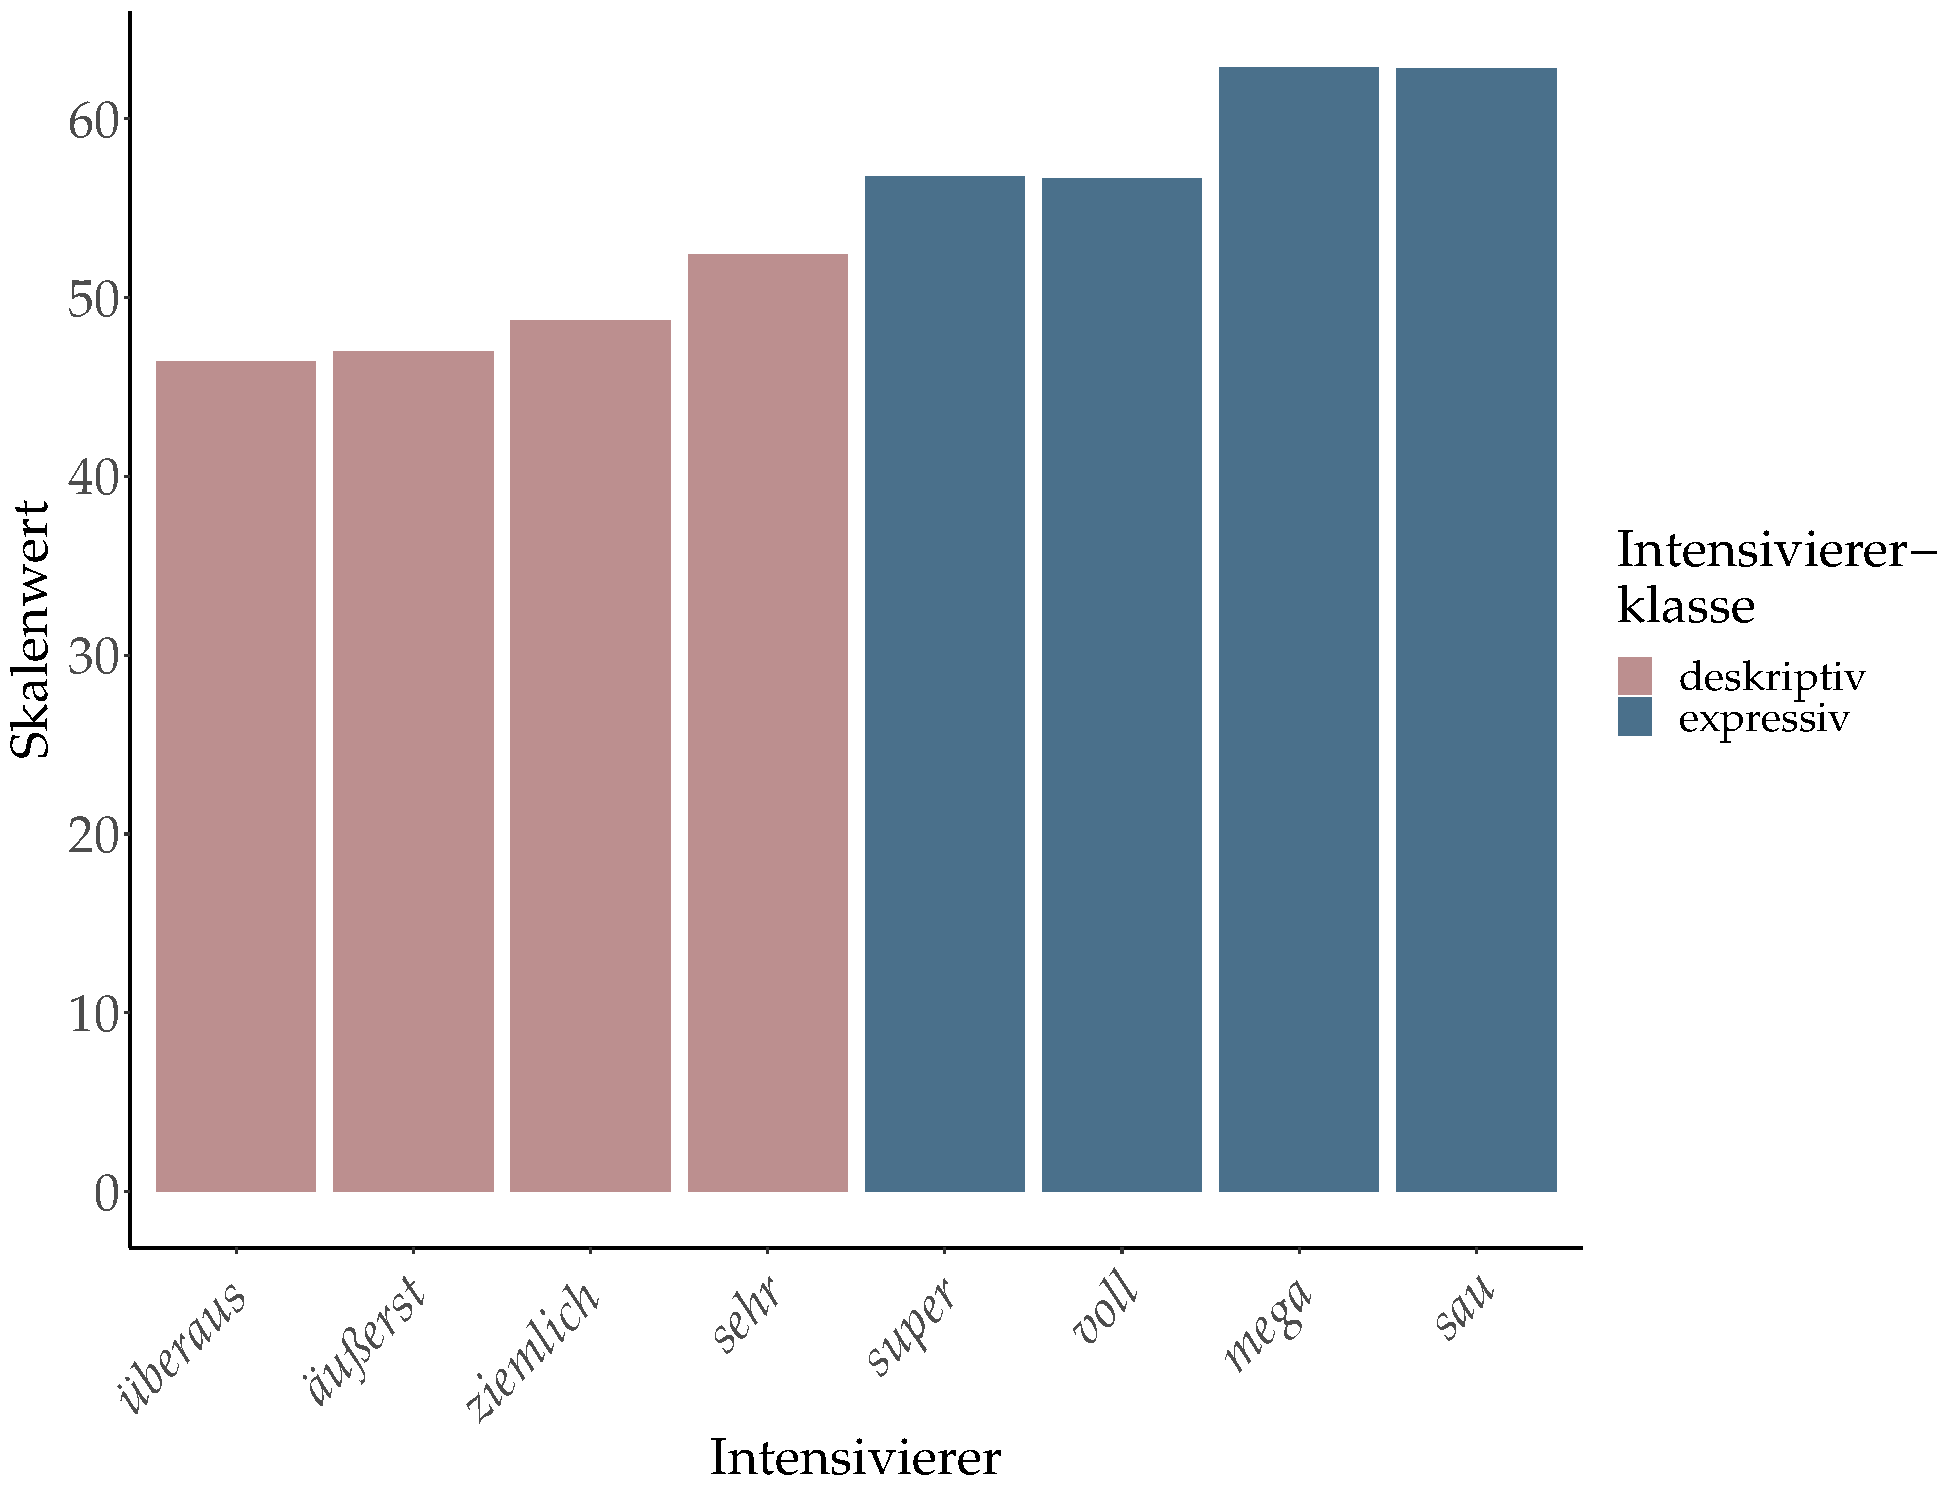
\includegraphics[width=1\textwidth]{Rplot_Bar_E2}
\caption[Säulendiagramm zu den einzelnen Intensivierern von Experiment 2b] {Säulendiagramm zu den einzelnen deskriptiven und expressiven Intensivierern von Experiment 2b -- Sprechereinstellung (x-Achse = Intensivierer, y-Achse = Skalenwert).}
\label{Bar2}
\end{figure}






\subsubsection{Paarweise Vergleiche der Intensivierer}\label{Paar2}


Wie weiter oben beschrieben, basierten die Paarvergleiche auf der Intention, die Unterschiede zwischen den einzelnen Ausdrücken auf Signifikanz hin zu überprüfen. Dazu wurden die einzelnen deskriptiven und expressiven Intensivierer analog zum Vorgehen bei Experiment 2a unter Zuhilfenahme des statistischen Modellierungsverfahrens \textit{t}-Test gepaart miteinander verglichen. In der daraus resultierenden Matrix bildet das überschneidende Element die Testprüfgröße \textit{t} sowie den jeweiligen Signifikanzwert \textit{p} ab. Auch hier wurde das Signifikanzniveau der $\alpha$-Adjustierung nach Bonferroni unterzogen, um die Alphafehler-Kumulierung zu eliminieren. Im Zuge dessen wurde der {\textit{p}-Wert} jedes kontrastierten Intensiviererpaars mit der Gesamtzahl der Vergleiche multipliziert. Die Gesamtzahl beträgt wie im vorherigen {Experiment 2a} 28, wurden doch alle Intensivierer paarweise miteinander gekreuzt: \textit{überaus} vs. \textit{äußerst}, \textit{überaus} vs. \textit{ziemlich}, \textit{überaus} vs. \textit{sehr}, \textit{überaus} vs. \textit{super}, \textit{überaus} vs. \textit{voll}, \textit{überaus} vs. \textit{mega}, \textit{überaus} vs. \textit{sau}, \textit{äußerst} vs. \textit{ziemlich}, \textit{äußerst} vs. \textit{sehr} usw. Durch die Multiplikation wird der jeweilige \textit{p}-Wert größer, sodass er entweder weniger oder auch überhaupt nicht mehr signifikant ist.


Die aus den Berechnungen resultierende Matrix ist in Tabelle \ref{Sign2_neu} dargestellt. Dabei werden zunächst die Vergleiche der deskriptiven Intensivierer (in ansteigendem Skalenwert) vorgenommen, an die sich die Vergleiche der expressiven Intensivierer (ebenfalls in ansteigendem Skalenwert sortiert) anschließen. Erneut sei klargestellt, dass bei den aufgelisteten \textit{t}-Werten aus Gründen der Darstellbarkeit von einer ausführlichen Dokumentation mit eingeklammerter Angabe der Anzahl der Freiheitsgrade, die auf der Größe der Stichprobe beruht, abgesehen wird {(\textit{t}\,(\textit{\textit{df}}) = \textelp{})}. Der Freiheitsgrad entspricht bei diesen Paarvergleichen dem Wert 3389. Insofern bedeutet die in der Tabelle jeweils aufgeführte verkürzte Form (z.\,B. {\textit{t} = -0,28}, {\textit{p} > 0,05}) streng genommen Folgendes: \textit{t}\,(3389) = \textelp{}, veranschaulicht am eingeklammerten Beispiel also {\textit{t}\,(3389) = -0,28}, {\textit{p} > 0,05}. Die Formel der paarweisen Vergleiche ist außerdem im Anhang \ref{Aja2} angegeben.




%\cellcolor[gray]{0.90}
%\cellcolor[gray]{0.75}
%\cellcolor[gray]{0.59}
%\hfil \ding{55}
%$\star$$\star$$\star$


%
\begin{sidewaystable}
\small
%\setlength{\tabcolsep}{8pt}

\begin{tabularx}{\textwidth}{l@{~~}QQQQ@{}Q@{}QQ@{}Q@{}}
\lsptoprule
Intensivierer & \textit{überaus} & \textit{äußerst} & \textit{ziemlich} & \textit{sehr} & \textit{super} & \textit{voll} & \textit{mega} & \textit{sau} \\
\midrule

\multirow{3}{*}{\textit{überaus}} &  &   \textit{t} = 0,28, & \textit{t} = 1,29, &  \cellcolor[gray]{0.59} \textit{t} = 3,92, & \cellcolor[gray]{0.59} \textit{t} = 6,47, &  \cellcolor[gray]{0.59} \textit{t} = 6,51, & \cellcolor[gray]{0.59}  \textit{t} = 10,62, &  \cellcolor[gray]{0.59} \textit{t} = 10,64, \\ 
& \hfil \ding{55} &   \textit{p} > 0,05   & \textit{p} > 0,05  & \cellcolor[gray]{0.59}  \textit{p} < 0,001 &   \cellcolor[gray]{0.59}  \textit{p} < 0,001  &   \cellcolor[gray]{0.59}  \textit{p} < 0,001   &   \cellcolor[gray]{0.59}  \textit{p} < 0,001    &  \cellcolor[gray]{0.59}  \textit{p} < 0,001    \\ 
 &  &  &  & \cellcolor[gray]{0.59} $\star$$\star$$\star$ & \cellcolor[gray]{0.59} $\star$$\star$$\star$ & \cellcolor[gray]{0.59} $\star$$\star$$\star$ & \cellcolor[gray]{0.59} $\star$$\star$$\star$ &  \cellcolor[gray]{0.59} $\star$$\star$$\star$ \\ 
 
\multirow{3}{*}{\textit{äußerst}} & \textit{t} = -0,28, &   & \textit{t} = 1,01, & \cellcolor[gray]{0.75} \textit{t} = 3,63, & \cellcolor[gray]{0.59} \textit{t} = 6,18, & \cellcolor[gray]{0.59}  \textit{t} = 6,22, &  \cellcolor[gray]{0.59} \textit{t} = 10,32, &  \cellcolor[gray]{0.59}  \textit{t} = 10,34, \\ 
&  \textit{p} > 0,05 &   \hfil \ding{55}   & \textit{p} > 0,05  & \cellcolor[gray]{0.75} \textit{p} < 0,01 &   \cellcolor[gray]{0.59}  \textit{p} < 0,001  &   \cellcolor[gray]{0.59}  \textit{p} < 0,001  &  \cellcolor[gray]{0.59}  \textit{p} < 0,001    &  \cellcolor[gray]{0.59}  \textit{p} < 0,001  \\ 
 &  &  &  & \cellcolor[gray]{0.75} $\star$$\star$ &  \cellcolor[gray]{0.59} $\star$$\star$$\star$ & \cellcolor[gray]{0.59} $\star$$\star$$\star$ & \cellcolor[gray]{0.59} $\star$$\star$$\star$ &  \cellcolor[gray]{0.59} $\star$$\star$$\star$ \\  
 
\multirow{3}{*}{\textit{ziemlich}} & \textit{t} = -1,29, &   \textit{t} = -1,01, &  &  \textit{t} = 2,63, & \cellcolor[gray]{0.59} \textit{t} = 5,18, & \cellcolor[gray]{0.59}  \textit{t} = 5,22, & \cellcolor[gray]{0.59} \textit{t} = 9,33, &  \cellcolor[gray]{0.59} \textit{t} = 9,35, \\ 
& \textit{p} > 0,05  &   \textit{p} > 0,05   & \hfil \ding{55}  & \textit{p} > 0,05 &  \cellcolor[gray]{0.59}  \textit{p} < 0,001  &   \cellcolor[gray]{0.59}  \textit{p} < 0,001  &   \cellcolor[gray]{0.59}  \textit{p} < 0,001  &  \cellcolor[gray]{0.59}  \textit{p} < 0,001   \\ 
 &  &  &  &  & \cellcolor[gray]{0.59} $\star$$\star$$\star$  & \cellcolor[gray]{0.59} $\star$$\star$$\star$ & \cellcolor[gray]{0.59} $\star$$\star$$\star$ &\cellcolor[gray]{0.59} $\star$$\star$$\star$   \\ 
 
\multirow{3}{*}{\textit{sehr}} & \cellcolor[gray]{0.59}  \textit{t} = -3,92, &  \cellcolor[gray]{0.75} \textit{t} = -3,63, & \textit{t} = -2,63, &   & \textit{t} = 2,56, &   \textit{t} = 2,59, & \cellcolor[gray]{0.59} \textit{t} = 6,70, &  \cellcolor[gray]{0.59} \textit{t} = 6,73, \\ 
&  \cellcolor[gray]{0.59}  \textit{p} < 0,001  &   \cellcolor[gray]{0.75} \textit{p} < 0,01    & \textit{p} > 0,05  & \hfil \ding{55}  &   \textit{p} > 0,05 &   \textit{p} > 0,05  &   \cellcolor[gray]{0.59}  \textit{p} < 0,001   &    \cellcolor[gray]{0.59}  \textit{p} < 0,001 \\ 
 & \cellcolor[gray]{0.59} $\star$$\star$$\star$ & \cellcolor[gray]{0.75} $\star$$\star$ &  &  &  &  & \cellcolor[gray]{0.59} $\star$$\star$$\star$ & \cellcolor[gray]{0.59} $\star$$\star$$\star$  \\ 
 
\multirow{3}{*}{\textit{super}} & \cellcolor[gray]{0.59} \textit{t} = -6,47, &  \cellcolor[gray]{0.59} \textit{t} = -6,18, &   \cellcolor[gray]{0.59}  \textit{t} = -5,18, & \textit{t} = -2,56, &  &   \textit{t} = 0,04, &   \cellcolor[gray]{0.59} \textit{t} = 4,14, &  \cellcolor[gray]{0.59}  \textit{t} = 4,17, \\ 
&  \cellcolor[gray]{0.59}  \textit{p} < 0,001  &    \cellcolor[gray]{0.59}  \textit{p} < 0,001    &   \cellcolor[gray]{0.59}  \textit{p} < 0,001   & \textit{p} > 0,05  &   \hfil \ding{55} &   \textit{p} > 0,05  &  \cellcolor[gray]{0.59}  \textit{p} < 0,001  &   \cellcolor[gray]{0.59}  \textit{p} < 0,001  \\ 
 & \cellcolor[gray]{0.59} $\star$$\star$$\star$ & \cellcolor[gray]{0.59} $\star$$\star$$\star$ & \cellcolor[gray]{0.59} $\star$$\star$$\star$ &  &  &  & \cellcolor[gray]{0.59} $\star$$\star$$\star$ &  \cellcolor[gray]{0.59} $\star$$\star$$\star$ \\  
 
\multirow{3}{*}{\textit{voll}} & \cellcolor[gray]{0.59} \textit{t} = -6,51, &  \cellcolor[gray]{0.59}  \textit{t} = -6,22, & \cellcolor[gray]{0.59} \textit{t} = -5,22, &  \textit{t} = -2,59, & \textit{t} = -0,04, &  &  \cellcolor[gray]{0.59} \textit{t} = 4,11, &  \cellcolor[gray]{0.59} \textit{t} = 4,14, \\ 
&  \cellcolor[gray]{0.59}  \textit{p} < 0,001   &  \cellcolor[gray]{0.59}  \textit{p} < 0,001    &  \cellcolor[gray]{0.59}  \textit{p} < 0,001  & \textit{p} > 0,05 &   \textit{p} > 0,05   &  \hfil \ding{55}   & \cellcolor[gray]{0.59}  \textit{p} < 0,001     &    \cellcolor[gray]{0.59}  \textit{p} < 0,001   \\ 
 & \cellcolor[gray]{0.59} $\star$$\star$$\star$ & \cellcolor[gray]{0.59} $\star$$\star$$\star$ & \cellcolor[gray]{0.59} $\star$$\star$$\star$ &  &  &  & \cellcolor[gray]{0.59} $\star$$\star$$\star$ &  \cellcolor[gray]{0.59} $\star$$\star$$\star$ \\ 
  
\multirow{3}{*}{\textit{mega}} & \cellcolor[gray]{0.59} \textit{t} = -10,62, &  \cellcolor[gray]{0.59} \textit{t} = -10,32, & \cellcolor[gray]{0.59} \textit{t} = -9,33, &  \cellcolor[gray]{0.59} \textit{t} = -6,70, & \cellcolor[gray]{0.59} \textit{t} = -4,14, &  \cellcolor[gray]{0.59} \textit{t} = -4,11, &   &   \textit{t} = 0,03, \\ 
&  \cellcolor[gray]{0.59}  \textit{p} < 0,001   &   \cellcolor[gray]{0.59}  \textit{p} < 0,001   &  \cellcolor[gray]{0.59}  \textit{p} < 0,001  & \cellcolor[gray]{0.59}  \textit{p} < 0,001    &  \cellcolor[gray]{0.59}  \textit{p} < 0,001 &   \cellcolor[gray]{0.59}  \textit{p} < 0,001  &   \hfil \ding{55}   &   \textit{p} > 0,05   \\ 
 &  \cellcolor[gray]{0.59} $\star$$\star$$\star$ & \cellcolor[gray]{0.59} $\star$$\star$$\star$ & \cellcolor[gray]{0.59} $\star$$\star$$\star$ & \cellcolor[gray]{0.59} $\star$$\star$$\star$ & \cellcolor[gray]{0.59} $\star$$\star$$\star$ & \cellcolor[gray]{0.59} $\star$$\star$$\star$ &  &   \\ 
 
\multirow{3}{*}{\textit{sau}} & \cellcolor[gray]{0.59} \textit{t} = -10,64, &  \cellcolor[gray]{0.59} \textit{t} = -10,34, & \cellcolor[gray]{0.59} \textit{t} = -9,35, & \cellcolor[gray]{0.59} \textit{t} = -6,73, & \cellcolor[gray]{0.59} \textit{t} = -4,17, &  \cellcolor[gray]{0.59} \textit{t} = -4,14, &  \textit{t} = -0,03, &    \\ 
&  \cellcolor[gray]{0.59}  \textit{p} < 0,001 &   \cellcolor[gray]{0.59}  \textit{p} < 0,001   & \cellcolor[gray]{0.59}  \textit{p} < 0,001   & \cellcolor[gray]{0.59}  \textit{p} < 0,001   & \cellcolor[gray]{0.59}  \textit{p} < 0,001   &    \cellcolor[gray]{0.59}  \textit{p} < 0,001   &  \textit{p} > 0,05   &   \hfil \ding{55}  \\ 
 & \cellcolor[gray]{0.59} $\star$$\star$$\star$ & \cellcolor[gray]{0.59} $\star$$\star$$\star$ & \cellcolor[gray]{0.59} $\star$$\star$$\star$ & \cellcolor[gray]{0.59} $\star$$\star$$\star$ &  \cellcolor[gray]{0.59} $\star$$\star$$\star$  & \cellcolor[gray]{0.59} $\star$$\star$$\star$  &  &   \\
\lspbottomrule

\end{tabularx}
\caption[Ergebnisse der Paarvergleiche der einzelnen Intensivierer von Experiment 2b]{Ergebnisse der Paarvergleiche der einzelnen Intensivierer bei Experiment 2b -- Sprechereinstellung (nach Bonferroni-Korrektur; angeordnet nach ansteigendem Skalenwert).}
\label{Sign2_neu}
\end{sidewaystable}



Die in Tabelle \ref{Sign2_neu} abgebildeten signifikanten Ergebnisse der Paarvergleiche werden nachfolgend knapp umrissen.\footnote{Auch hier wird der signifikante \textit{p}-Wert lediglich bei der ersten Erwähnung eines kontrastierten Intensiviererpaars aufgeführt (z.\,B. \textit{überaus} vs. \textit{sehr}), während er bei der Zweitnennung außen vor gelassen wird (\textit{sehr} vs. \textit{überaus}).} Begonnen wird mit den Vergleichen des am niedrigsten positionierten deskriptiven Intensivierers \textit{überaus}. Hier sind signifikante Unterschiede bei den Kontrasten mit \textit{sehr} ({\textit{t}\,(3389) = 3,92}, \textit{p} < 0,001), \textit{super} (\textit{t}\,(3389) = 6,47, \textit{p} < 0,001), \textit{voll} (\textit{t}\,(3389) = 6,51, {\textit{p} < 0,001}), \textit{mega} (\textit{t}\,(3389) = 10,62, \textit{p} < 0,001) und  \textit{sau} ({\textit{t}\,(3389) = 10,64}, {\textit{p} < 0,001)} auszumachen. Der nächste deskriptive Intensivierer ist \textit{äußerst}. Dieser Ausdruck weist gleichfalls signifikante Unterschiede bei den Vergleichen mit \textit{sehr} (\textit{t}\,(3389) = 3,63, {\textit{p} < 0,01)}, \textit{super} (\textit{t}\,(3389) = 6,18, \textit{p} < 0,001), \textit{voll} ({\textit{t}\,(3389) = 6,22}, {\textit{p} < 0,001}), \textit{mega} {(\textit{t}\,(3389) = 10,32}, \textit{p} < 0,001) und \textit{sau} ({\textit{t}\,(3389) = 10,34}, {\textit{p} < 0,001)} auf. Bei \textit{ziemlich} sind signifikante Unterschiede bei den Kontrasten mit \textit{super} {(\textit{t}\,(3389) = 5,18,} \textit{p} < 0,001), \textit{voll} (\textit{t}\,(3389) = 5,22, {\textit{p} < 0,001}), \textit{mega} (\textit{t}\,(3389) = 9,33, {\textit{p} < 0,001}) und \textit{sau} {(\textit{t}\,(3389) = 9,35,} {\textit{p} < 0,001}) zu beobachten. Als Nächstes werden die Ergebnisse des am höchsten eingestuften deskriptiven Intensivierers \textit{sehr} begutachtet, die bei \textit{überaus}, \textit{äußerst}, \textit{mega} (\textit{t}\,(3389) = 6,70, {\textit{p} < 0,001)} und \textit{sau} ({\textit{t}\,(3389) = 6,73}, {\textit{p} < 0,001}) signifikant sind. Den Resultaten der paarweisen Vergleiche nach zu urteilen, unterscheiden sich also drei deskriptive Intensivierer gänzlich von den untersuchten expressiven Intensivierern, was im Anschluss zu diskutieren ist: \textit{überaus}, \textit{äußerst} {und \textit{ziemlich}}.


Bei den expressiven Intensivierern wird mit den Ergebnissen der Kontraste von \textit{super} begonnen, die bei \textit{überaus}, \textit{äußerst}, \textit{ziemlich}, \textit{mega} ({\textit{t}\,(3389) = 4,14}, {\textit{p} < 0,001})  und \textit{sau} ({\textit{t}\,(3389) = 4,17}, {\textit{p} < 0,001}) signifikant sind. Gleichsam zeigt auch \textit{voll} signifikante Unterschiede bei den Kontrasten mit \textit{überaus}, \textit{äußerst}, \textit{ziemlich}, \textit{mega} ({\textit{t}\,(3389) = 4,11}, {\textit{p} < 0,001}) und \textit{sau} ({\textit{t}\,(3389) = 4,14}, {\textit{p} < 0,001}) auf. Der nächste expressive Intensivierer in der Reihe ist \textit{mega}. Wie bereits beschrieben, sind bei diesem Ausdruck signifikante Unterschiede bei den Vergleichen mit \textit{überaus}, \textit{äußerst}, \textit{ziemlich}, \textit{sehr}, \textit{super} und \textit{voll} zu erkennen, genauso wie sich der höchstplatzierte expressive Intensivierer \textit{sau} signifikant von den soeben genannten Intensivierern unterscheidet.


Von den Ergebnissen der Paarvergleiche ausgehend kann geschlussfolgert werden, dass sich zwei Intensivierer klar im Hinblick auf den ihnen zugeschriebenen Grad an Sprechereinstellung von den restlichen Intensivierern unterscheiden, nämlich \textit{mega} und \textit{sau}. Die Kontraste dieser Ausdrücke sind in sechs von sieben Fällen signifikant. Die inter- und intraklassischen Unterschiede der vorgenommenen Vergleiche werden in Abschnitt \ref{abs:Diskussion2} diskutiert.








%
\subsection{Diskussion}\label{abs:Diskussion2}
Nachfolgend werden die Ergebnisse von Experiment 2b besprochen und mit Blick auf die oben beschriebene Hypothese  H6 bewertet. Nach dieser ist von graduellen Abstufungen innerhalb der Intensiviererklassen auszugehen, die auf die Semantik der Ausdrücke zurückzuführen sind (vgl. {\citealt[87]{Biedermann.1969}}; \citealt[408]{Breindl.2007}). Im Sinne von \citet[133]{Gutzmann.2019a} besteht außerdem die Möglichkeit, dass die Expressivität der Intensivierer auf deren Skalaritätsgrad einwirkt, letzterer infolge der Expressivität als stärker wahrgenommen wird und die beiden Variablen \textsc{Skalarität} und \textsc{Sprechereinstellung} miteinander korrelieren. Da es sinnvoll ist, {Experiment 2a}, das zur Erhebung des Skalaritätsgrades durchgeführt wurde, und das soeben geschilderte Experiment 2b in ihrer Gesamtheit zu betrachten, erfolgt die finale Ergebnisinterpretation erst in Abschnitt \ref{abs:Gesamtdiskussion}.


In Experiment 2b ging es für die Versuchspersonen darum, mithilfe eines Schiebereglers auf einer Skala von `gar nicht bewertend' bis `maximal bewertend' den im Satz enthaltenen Grad an Sprechereinstellung einzuschätzen, bspw. \textit{Wie bewertend ist die Aussage \glqq{}Der Berg ist äußerst hoch\grqq{}?}


Bei der Begutachtung der Intensiviererklassen stellte sich heraus, dass Sätze mit expressiven Intensivierern von den Versuchspersonen mit einem signifikant höheren Grad an Sprechereinstellung assoziiert wurden als Sätze mit deskriptiven Intensivierern (vgl. Tabelle \ref{LinReg2}). Wie schon in dem in Kapitel \ref{Experiment0} besprochenen Experiment 1 erhärtet dieser Befund das Zutreffen der Annahme eines wahrnehmbaren Unterschiedes in der Expressivität von deskriptiven und expressiven Intensivierern (vgl. die Hypothese H4 nach {\citealt[315]{Lang.1983}} und \citealt[57]{Ortner.2014}). Den Ergebnissen der beiden Untersuchungen nach zu urteilen, wurde der Grad an Sprechereinstellung bei expressiven Intensivierern als signifikant stärker empfunden als bei deskriptiven Intensivierern, was als weitere Evidenz für die Gültigkeit der {Hypothese H4} herangezogen werden kann. Dennoch ergibt sich die Frage, wieso die untersuchten deskriptiven Intensivierer trotz fehlender Expressivität nicht mit einem noch niedrigeren Grad an Sprechereinstellung verbunden wurden. So ist gemäß der Definition von \citet[133]{Gutzmann.2019a} anzunehmen, dass deskriptive Intensivierer -- anders als expressive Intensivierer -- überhaupt keine Sprechereinstellung ausdrücken und daher am unteren Ende einer kontinuierlichen Skala verortet werden. Eine solch niedrige Skaleneinschätzung zeigte sich in {Experiment 2b} jedoch nicht. Infolgedessen sind die Ergebnisse insofern bemerkenswert, als sie zu bedenken geben, dass deskriptive Intensivierer durchaus als einstellungsausdrückend wahrgenommen werden, wenn auch nicht dergestalt, dass sie an die expressiven Intensivierer heranreichen.


Auch für diese Untersuchung waren die in der theoretischen Literatur angenommenen intraklassischen Abstufungen zentral, weswegen die Intensiviererklassen im nächsten Analyseschritt aufgetrennt und ihre Mitglieder im Detail begutachtet wurden. Erneut waren klasseninterne Abstufungen auszumachen: \textit{überaus}|\textit{äußerst} $\prec$ \textit{ziemlich} $\prec$ \textit{sehr} sowie \textit{super}|\textit{voll} $\prec$ \textit{mega}|\textit{sau}. Somit gibt es Ausdrücke, die sich nach dem Empfinden der Versuchspersonen in Hinsicht auf Sprechereinstellung gleichen: \textit{überaus} und \textit{äußerst} aufseiten der deskriptiven Intensivierer und \textit{super} und \textit{voll} sowie \textit{mega} und \textit{sau} aufseiten der expressiven Intensivierer. Das bedeutet, dass die Ergebnisse von Experiment 2b im Wesentlichen ebenso für die zu untersuchende {Hypothese H6} sprechen. Trotz der Abstufungen unterscheidet sich die beobachtete Rangfolge nahezu gänzlich von der, die sich im Kontext der in {Experiment 2a} erfragten Skalarität zeigte. Wurde der deskriptive Intensivierer \textit{ziemlich} in {Experiment 2a} mit dem niedrigsten Skalaritätsgrad assoziiert, wurde der mit ihm einhergehende Grad an Sprechereinstellung in Experiment 2b hingegen umso höher beurteilt. Auch wenn der Ausdruck nicht übermäßig skalierend zu sein scheint, wird er dennoch als vergleichsweise stark bewertend wahrgenommen. Gegenteiliges trifft auf den deskriptiven Intensivierer \textit{überaus} zu, dem im Kontext der Skalarität von den Versuchspersonen der höchste Grad zugeschrieben wurde. Die Ergebnisse von {Experiment 2b} weisen jedoch darauf hin, dass der Ausdruck bloß als schwach einstellungsausdrückend empfunden wird. Die Position des deskriptiven Intensivierers \textit{äußerst} ist gleich geblieben, wurde der Ausdruck doch sowohl bezüglich Skalarität als auch Sprechereinstellung an zweiter Stelle verortet. Während das deskriptive \textit{sehr} bereits mit einem hohen Skalaritätsgrad in Verbindung gebracht wurde, wurde der durch ihn ausgedrückte Grad an Sprechereinstellung noch höher eingeschätzt, was dazu führt, dass der Ausdruck diesbezüglich die höchste Skalenposition innerhalb der deskriptiven Intensiviererklasse einnimmt. Daneben hat sich die Rangfolge innerhalb der expressiven Klasse ebenfalls geändert, wenn auch in erster Linie in dem Sinne, dass die Ausdrücke den Platz mit ihrem Nachbarn getauscht haben. Die soeben dargelegten Unterschiede, die in Bezug auf die Einschätzung von Skalarität und Sprechereinstellung auszumachen sind, legen in Summe nahe, dass die Untersuchungsmethode funktioniert hat und die Versuchspersonen die beiden Merkmale unterschiedlich wahrgenommen und {evaluiert haben}.


Aus der Intention heraus die festgestellten Unterschiede auf Signifikanz hin zu überprüfen, wurden die Intensivierer daraufhin gepaart miteinander verglichen (vgl. Tabelle \ref{Sign2_neu}). In diesem Kontext zeigte sich nicht nur eine signifikante Zweiteilung der Ausdrücke nach deskriptiv und expressiv, sondern auch, dass sich fast alle der ähnlich eingestuften Ausdrücke angesichts der Signifikanzen parallel verhalten. Dabei unterscheiden sich vor allem zwei Intensivierer klar im Hinblick auf den ihnen zugesprochenen Grad an Sprechereinstellung, nämlich \textit{mega} und \textit{sau}. Deren Vergleiche sind in sechs von sieben Fällen signifikant: bei allen deskriptiven Intensivierern, d.\,h. bei \textit{überaus}, \textit{äußerst}, \textit{ziemlich} und \textit{sehr}, sowie den expressiven Intensivierern \textit{super} und \textit{voll}. Lediglich die Gegenüberstellung der beiden Ausdrücke ist nicht signifikant, was durch die ähnliche Skaleneinschätzung bedingt ist. Wie sind die signifikanten Unterschiede zu erklären? Der Intensivierer \textit{sau} wurde bereits im Kontext der Skalarität als vergleichsweise hoch empfunden und so wurde er ebenso bezüglich Sprechereinstellung auf der Skala an höchster Position verortet. Bei diesem Ausdruck ist, wie oben beschrieben, denkbar, dass dieses Ergebnis der transparenten Semantik und der damit verbundenen derben Konnotation geschuldet ist, die möglicherweise zur hohen Gradeinschätzung beigetragen haben. Dagegen scheint bei \textit{mega} vor allem die Aktualität des Ausdrucks auf die Wahrnehmung einzuwirken, in deren Folge er gleichermaßen als übermäßig skalar und stark expressiv empfunden wird. Dies wirft die Frage auf, wie die Expressivität von \textit{mega} in ein paar Jahren eingeschätzt wird, sollte der Ausdruck bis dahin inflationär im Gebrauch sein. Ähnliches ist bei den Kontrasten der expressiven Intensivierer \textit{voll} und \textit{super} zu beobachten, deren Vergleiche aufgrund ähnlicher Skalenwerte ebenfalls zu gleichen signifikanten Ergebnissen führten. Diese treten in fünf von sieben Fällen auf: bei den deskriptiven Intensivierern \textit{überaus}, \textit{äußerst} und \textit{ziemlich} sowie den am höchsten eingeschätzten expressiven Intensivierern \textit{mega} und \textit{sau}. Dies deutet darauf hin, dass \textit{super} und \textit{voll} zwar als expressiver wahrgenommen werden als die deskriptiven Intensivierer, der durch sie ausgedrückte Grad an Sprechereinstellung jedoch nicht an \textit{mega} und \textit{sau} heranreicht. Auch innerhalb der deskriptiven Intensiviererklasse zeichnen sich infolge ähnlicher Skaleneinschätzung parallele Signifikanzen ab, sind die Ergebnisse der Paarvergleiche von \textit{äußerst} und \textit{überaus} doch in fünf von sieben Fällen signifikant: bei dem in Bezug auf Sprechereinstellung am höchsten eingeschätzten deskriptiven Intensivierer \textit{sehr} sowie den expressiven Intensivierern \textit{super}, \textit{voll}, \textit{mega} und \textit{sau}. Somit unterscheiden sich die niedrig bewerteten deskriptiven Intensivierer \textit{äußerst} und \textit{überaus} nicht nur signifikant von allen expressiven Intensivierern, sondern auch von dem am höchsten positionierten deskriptiven Intensivierer \textit{sehr}. Weil der Grad an Sprechereinstellung bei \textit{sehr} von den Versuchspersonen im Mittelfeld der Skala angesiedelt wurde, sind seine Vergleiche in vier Fällen signifikant: bei \textit{äußerst} und \textit{überaus} sowie den expressiven Intensivierern \textit{mega} und \textit{sau}. Der im Kontext der Sprechereinstellung vergleichsweise hoch eingeschätzte deskriptive Intensivierer \textit{ziemlich} unterscheidet sich hingegen signifikant von allen expressiven Intensivierern, d.\,h. von \textit{super}, \textit{voll}, \textit{mega} und \textit{sau}.


Auf Grundlage der Ergebnisse von Experiment 2b lässt sich schlussfolgern, dass die zu überprüfende Hypothese H6 im Kern korrekt ist. Denn auch in dieser Untersuchung treten in beiden Intensiviererklassen graduelle Abstufungen bezüglich des mit den Ausdrücken assoziierten Grades an Sprechereinstellung auf: schwach $\prec$ mittel $\prec$ stark. 
%In diesem Sinne können die Intensiviererklassen auf zwei verschiedenen Skalen nebeneinander geordnet werden. Wie bereits bei Skalarität wird dies in Tabelle \ref{stark} verbildlicht. Auch hier erfolgt die Anordnung der Intensiviererklassen in ansteigendem Skalenwert.



%%
%\begin{table}[h]
%
%%\setlength{\tabcolsep}{8.25pt}
%%\begin{tabular}{p{0.15\textwidth} p{0.1\textwidth} p{0.15\textwidth} p{0.1\textwidth} p{0.15\textwidth}}
%\begin{tabularx}{.8\textwidth}{Xlclc}
%\lsptoprule
% & & \multicolumn{2}{c}{\textbf{Intensiviererklasse}}  \\ [0.5em]
%\multirow{2}{*}{Stärkegrad} & \multicolumn{2}{c}{\textsc{deskriptiv}} & \multicolumn{2}{c}{\textsc{expressiv}}  \\ 
% & Intensivierer & Skalenwert & Intensivierer & Skalenwert  \\ 
%  &  & (\textit{SD})  &  & (\textit{SD})  \\
%\midrule 
%\\
%schwach & \textit{überaus} & 46,99 & \textit{super} & 57,15  \\
% & & (27.4) & & (28.2)  \\
% & \textit{äußerst} & 47,40 & \textit{voll} & 57,23 \\
%& & (25.7) &  & (27.8)\\
%\multicolumn{1}{l}{mittel} & \textit{ziemlich} & 49,06 & \textit{mega} & 63,67\\
%  & & (28.2) & & (28.0)\\
%stark & \textit{sehr} & 53,15 & \textit{sau} & 63,69  \\
% & & (29.6) & & (29.4)  \\
%\end{tabularx}
%\caption[Klasseninterne graduelle Abstufungen bei Experiment 2b]{Klasseninterne graduelle Abstufungen bei Experiment 2b -- Sprechereinstellung (in ansteigendem Skalenwert).}
%\label{stark}
%\end{table}









%
%\subsubsection{Paarweise Vergleiche der Intensivierer}\label{abs:Intensiviererpaarvergl} $~$ \\
%Die aus den Ergebnissen der Paarvergleiche resultierende Matrix deutete auf den ersten Blick auf eine signifikante Zweiteilung der Intensivierer nach deskriptiv und expressiv hin (vgl. Tabelle \ref{Sign2}). So zeigten nahezu alle Intensivierer signifikante Unterschiede bei den Vergleichen mit der gegenteiligen Intensiviererklasse, d.\,h. deskriptiv vs. expressiv und expressiv vs. deskriptiv. Die einzige Ausnahme stellte der deskriptive Intensivierer \textit{sehr} dar: Der gemittelte Skalenwert dieses Ausdrucks lag mit 53,15 Punkten nahe beim am niedrigsten positionierten expressiven Intensivierer \textit{super}, der auf der Skala im Schnitt bei 57,15 Punkten angesiedelt wurde ($\Delta$ = ca. 4,00 Punkte). Infolgedessen war der Unterschied zwischen \textit{sehr} und \textit{super} ebenso wie zwischen \textit{sehr} und \textit{sau} nicht signifikant. Durch den vergleichsweise hohen Skalenwert unterschied sich \textit{sehr} überdies signifikant von den deskriptiven Intensivierern {\textit{äußerst} (47,40 Punkte)} und \textit{überaus} (46,99 Punkte), dessen denkbare Ursachen oben diskutiert wurden. Ähnliches war innerhalb der expressiven Intensiviererklasse auszumachen, in der sich die beiden höchstpositionierten Ausdrücke {\textit{mega} (63,67 Punkte)} und \textit{sau} (63,69 Punkte) signifikant von den niedrigpositionierten Ausdrücken \textit{super} (57,15 Punkte) und \textit{voll} {(57,23 Punkte)} unterschieden. Die möglichen Gründe hierfür wurden ebenfalls im vorherigen Abschnitt beschrieben.


%Zusammengenommen zeigten die Ergebnisse der paarweisen Vergleiche im Hinblick auf die in Experiment 2b untersuchte Sprechereinstellung einen stark ausgeprägten Unterschied zwischen den Intensiviererklassen.






%Diese werden im Anschluss der Reihe nach erörtert. Begonnen wird mit dem deskriptiven Intensiviererpaar \textit{überaus} (46,99 Punkte) und \textit{äußerst} (47,40 Punkte), das transparente Ausdrücke beinhaltet, deren lexikalischer Ursprung deutlich wahrnehmbar ist {($\Delta$ = ca. 0,41 Punkte)}. Semantisch denotieren die Intensivierer einen bestimmten Punkt, der entweder angenähert oder überschritten wird. Überraschend ist insbesondere der gemittelte Skalenwert von \textit{überaus}, handelte es sich in Experiment 2a dabei doch um denjenigen deskriptiven Intensivierer, dessen Skalaritätsgrad von den Versuchspersonen auf der Skala am höchsten bewertet wurde. Dieses Ergebnis wurde auf eine niedrige Gebrauchsfrequenz zurückgeführt, die sich offenbar in einer höheren Einstufung des Intensivierers auf der Skala niedergeschlagen hat. Daraus lässt sich ableiten, dass der Ausdruck zwar mit einem hohen Grad an Skalarität assoziiert wird, der durch ihn ausgedrückte Grad an Sprechereinstellung allerdings als verhältnismäßig niedrig empfunden wird. Gegenläufig dazu wurde der Skalaritätsgrad von \textit{äußerst} in {Experiment 2a} niedriger eingestuft, was durch eine hohe Gebrauchsfrequenz erklärt wurde. Während sich \textit{überaus} im Korpus mit 10\,534 absoluten Treffern belegen lässt, ist \textit{äußerst} mit 19\,723 Treffern darin fast doppelt so häufig vertreten. Dessen ungeachtet wurden die beiden Ausdrücke in {Experiment 2b} im Hinblick auf Sprechereinstellung auf der Skala vergleichbar evaluiert, was zeigt, dass sie von den Versuchspersonen gleichermaßen als nur wenig einstellungsausdrückend wahrgenommen wurden. Genauso unerwartet war das Ergebnis von \textit{sehr}, dem innerhalb der deskriptiven Intensiviererklasse der höchste Skalenwert zugeschrieben wurde. Dies lässt den Schluss zu, dass \textit{sehr} nicht, wie in der theoretischen Literatur mitunter behauptet (bspw. \citealt[7]{Mueller.1899}; {\citealt[365]{Claudi.2006}}), notwendig nur moderat intensivierend ist.\footnote{Hiervon ist natürlich das aus pragmatischen Gründen reduplizierte \textit{sehr} zu trennen, das ohnehin einen stärkeren Intensitätsgrad ausdrückt als das einfache \textit{sehr} (vgl. u.\,a. {\citealt[16f.]{Hauschild.1899}}; \citealt[266]{Becher.1907}; \citealt[191]{Staffeldt.2018}).} Stattdessen deutet die Einschätzung von \textit{sehr} vielmehr auf einen ungewöhnlich hohen Grad an Sprechereinstellung hin, dessen Ursache möglicherweise in der Opazität des Ausdrucks begründet ist. So legten die Ergebnisse der deskriptiven Intensivierer nahe, dass semantische Transparenz für die kommunizierte Sprechereinstellung eher hemmend ist, während semantische Opazität dagegen mutmaßlich zu einem höheren Skalenwert führt. Innerhalb der expressiven Intensiviererklasse zeichnete sich hinsichtlich Sprechereinstellung eine klare zweiteilige Abstufung ab (vgl. Abbildung \ref{Bar2}). Diese äußerte sich darin, dass das Intensiviererpaar {\textit{super} (57,15 Punkte)} und \textit{voll} {(57,23 Punkte)} von den Versuchspersonen ähnlich bewertet wurde {($\Delta$ = ca. 0,08 Punkte)}, ebenso wie auch \textit{mega} (63,67 Punkte) und \textit{sau} (63,69 Punkte) eine nahezu gleichwertige Skalenposition zugewiesen wurde {($\Delta$ = ca. 0,02 Punkte)}. Während \textit{voll} bereits in Experiment 2a in Bezug auf Skalarität niedrig gerankt wurde, wies \textit{super} erst bei der in {Experiment 2b} untersuchten Sprechereinstellung einen vergleichsweise niedrigen Skalenwert auf. Demnach deuten die Ergebnisse darauf hin, dass \textit{super} nach Einschätzung der Versuchspersonen zwar mit einem mittleren Skalaritätsgrad einhergeht, der durch ihn ausgedrückte Grad an Sprechereinstellung jedoch eher niedrig ist. Dies ist schätzungsweise dem starken Lexikalisierungsgrad und der dementsprechend hohen Gebrauchsfrequenz geschuldet, die dazu führten, dass \textit{super} mit 391,26 Treffern pro Million Textwörter der häufigste Intensivierer im Korpus ist. Dadurch ist es naheliegend, dass der Ausdruck inzwischen als nicht mehr übermäßig expressiv wahrgenommen wird und er in der Folge mit Blick auf Sprechereinstellung von den Versuchspersonen auf der Skala niedrig verortet wurde. Ähnliches ist bei \textit{voll} vorstellbar: Auch wenn der Ausdruck im Korpus lediglich 36,65 Treffer pro Million Textwörter aufweist, ist er aufgrund seines langen Gebrauchs eventuell zu abgenutzt, um als stark expressiv beurteilt zu werden. Das Ergebnis von \textit{voll} steht zudem im Einklang mit den Resultaten des in {Kapitel \ref{Experiment0}} vorgestellten Experiments: Auch darin wurde dem intensivierenden \textit{voll} von den Versuchspersonen weder in Bezug auf Skalarität noch auf Sprechereinstellung ein hoher Grad zugesprochen (vgl. die {Tabellen \ref{SkaWe2} und \ref{SkaWey}}). Neben \textit{super} und \textit{voll} wurden die im Korpus niedrigfrequenten Intensivierer \textit{mega} und \textit{sau} in {Experiment 2b} fast äquivalent bewertet. Dieses Paar bildete die zweite Stufe innerhalb der expressiven Intensiviererklasse. Festzustellen war außerdem, dass beide Ausdrücke schon im Hinblick auf Skalarität ähnlich hoch lokalisiert wurden (vgl. {Tabelle \ref{Skalenwert3}}), was bedeutet, dass sie von den Versuchspersonen sowohl im Kontext von Skalarität als auch von Sprechereinstellung mit einem hohen Grad assoziiert wurden. Dieser Befund liefert weitere Evidenz für die zu testenden Hypothesen, nach denen sich Expressivität in Form eines höheren Grades an Skalarität und Sprechereinstellung manifestiert (vgl. {\citealt[315]{Lang.1983}}; {\citealt[22]{Paradis.1997}}; {\citealt[57]{Ortner.2014}}; \citealt[133]{Gutzmann.2019a}). Bei \textit{mega} wurde der hohe Skalenwert durch die anhaltende Aktualität erklärt, die gegebenenfalls dazu führt, dass der Ausdruck als ausdrucksstärker wahrgenommen wird als bspw. der dem Anschein nach abgenutzte Intensivierer \textit{voll}. Ursächlich für den hohen Skalenwert von \textit{sau} war potenziell die klar erkennbare Semantik und die damit verbundene derbe Konnotation, die bereits bei dem in Kapitel \ref{Experiment0} geschilderten Experiment zu einem vergleichbaren Ergebnis bzw. einem als hoch eingeschätzten Grad an Sprechereinstellung beigetragen hat.
%Angesichts der bereits gewonnenen Ergebnisse ist die Zweiteilung, die sich innerhalb der expressiven Intensiviererklasse beobachten lässt, wenig überraschend und erhärtet diese nachdrücklich.





%\subsubsection{Paarweise Vergleiche der Intensivierer}\label{abs:Intensiviererpaarvergl} $~$ \\
%Die aus den Ergebnissen der Paarvergleiche resultierende Matrix deutete auf den ersten Blick auf eine signifikante Zweiteilung der Intensivierer nach deskriptiv und expressiv hin (vgl. Tabelle \ref{Sign2}). So zeigten nahezu alle Intensivierer signifikante Unterschiede bei den Vergleichen mit der gegenteiligen Intensiviererklasse, d.\,h. deskriptiv vs. expressiv und expressiv vs. deskriptiv. Die einzige Ausnahme stellte der deskriptive Intensivierer \textit{sehr} dar: Der gemittelte Skalenwert dieses Ausdrucks lag mit 53,15 Punkten nahe beim am niedrigsten positionierten expressiven Intensivierer \textit{super}, der auf der Skala im Schnitt bei 57,15 Punkten angesiedelt wurde ($\Delta$ = ca. 4,00 Punkte). Infolgedessen war der Unterschied zwischen \textit{sehr} und \textit{super} ebenso wie zwischen \textit{sehr} und \textit{sau} nicht signifikant. Durch den vergleichsweise hohen Skalenwert unterschied sich \textit{sehr} überdies signifikant von den deskriptiven Intensivierern {\textit{äußerst} (47,40 Punkte)} und \textit{überaus} (46,99 Punkte), dessen denkbare Ursachen oben diskutiert wurden. Ähnliches war innerhalb der expressiven Intensiviererklasse auszumachen, in der sich die beiden höchstpositionierten Ausdrücke {\textit{mega} (63,67 Punkte)} und \textit{sau} (63,69 Punkte) signifikant von den niedrigpositionierten Ausdrücken \textit{super} (57,15 Punkte) und \textit{voll} {(57,23 Punkte)} unterschieden. Die möglichen Gründe hierfür wurden ebenfalls im vorherigen Abschnitt beschrieben.


%Zusammengenommen zeigten die Ergebnisse der paarweisen Vergleiche im Hinblick auf die in Experiment 2b untersuchte Sprechereinstellung einen stark ausgeprägten Unterschied zwischen den Intensiviererklassen.






 





\section{Ergebnisinterpretation}\label{abs:Gesamtdiskussion}
Im Anschluss werden die Ergebnisse der beiden Experimente zusammengefasst, miteinander verzahnt und hinsichtlich der zentralen {Hypothese H6} evaluiert. Wie in Abschnitt \ref{abs:theo} beschrieben, wurde die Untersuchung mit dem Ziel vorgenommen, möglichen Unterschieden zwischen Intensivierern erstmals mit experimentellen Methoden auf den Grund zu gehen. In diesem Zusammenhang wurde die Überprüfung einer Annahme angestrebt, die sich aus den von {\citet[87]{Biedermann.1969}} und \citet[408]{Breindl.2007} postulierten intraklassischen Abstufungen ergibt. Von diesem Standpunkt aus ist anzunehmen, dass sich graduelle Abstufungen in den Stärkegraden von Intensivierern zeigen und sich die Mitglieder einer Intensiviererklasse im Hinblick auf den durch sie ausgedrückten Grad an Skalarität und Sprechereinstellung voneinander unterscheiden. Um die Korrektheit der {Hypothese H6} empirisch zu testen, wurden zwei Rating-Experimente mit parallelem Untersuchungsaufbau durchgeführt: Während {Experiment 2a} den Grad an Skalarität erfragte, zielte {Experiment 2b} auf den Grad an {Sprechereinstellung ab}.


%\subsection{Experiment 2a und Experiment 2b}\label{abs:Gesamtdiskuss}
Sowohl die Ergebnisse von Experiment 2a wie auch die von {Experiment 2b} sprechen in erster Linie klar für einen wahrnehmbaren Unterschied zwischen deskriptiven und expressiven Intensivierern. So positionierten die Versuchspersonen Sätze mit expressiven Intensivierern in beiden Kontexten signifikant höher als Sätze mit deskriptiven Intensivierern. Dies bekräftigt die grundlegende Annahme, dass Expressivität gleichermaßen mit einem höheren Grad an Skalarität und Sprechereinstellung einhergeht (vgl. {\citealt[315]{Lang.1983}}; \citealt[22]{Paradis.1997}; {\citealt[57]{Ortner.2014}}; {\citealt[133]{Gutzmann.2019a}}). Darüber hinaus stimmt es mit den Ergebnissen überein, die durch die in Kapitel \ref{Experiment0} vorgestellte Untersuchung in Bezug auf die darin getesteten Hypothesen H3 und H4 zutage gebracht werden konnten.


Da in dieser Untersuchung vor allem die potenziellen klasseninternen Abstufungen zentral waren, wurden die beiden Intensiviererklassen im nächsten Schritt ausdifferenziert und ihre Mitglieder detailliert begutachtet. Die Klassen werden im Folgenden der Reihe nach inspiziert. Begonnen wird mit den deskriptiven Intensivierern. Für einen besseren Überblick sind die gemittelten Skalenwerte und Standardabweichungen für die {Experimente 2a und 2b} in {Tabelle \ref{deIn}} zusammengefasst.
%Die Anordnung der Intensivierer erfolgt jeweils in ansteigendem Skalenwert.


\begin{table}
\small
%\setlength{\tabcolsep}{8.25pt}
%\begin{tabular}{p{0.15\textwidth} p{0.1\textwidth} p{0.15\textwidth} p{0.1\textwidth} p{0.15\textwidth}}
\begin{tabularx}{\textwidth}{X@{} lrr lrr }
\lsptoprule
 &  \multicolumn{6}{c}{\textbf{Deskriptive Intensivierer}}  \\
\cmidrule(lr){2-7}\cmidrule(lr){5-7}
& \multicolumn{3}{c}{{Skalarität}} & \multicolumn{3}{c}{{Sprechereinstellung}}  \\
\cmidrule(lr){2-4}\cmidrule(lr){5-7}
{Stärkegrad}  & Intensivierer & Skalenwert& \textit{SD}  & Intensivierer & Skalenwert& \textit{SD}   \\
\midrule
schwach & \textit{ziemlich} & 51,22& 23,6 & \textit{überaus} & 46,99 & 27,4  \\
 & & &  &    \textit{äußerst} & 47,40& 25,7 \\
mittel & \textit{äußerst} & 59,46& 23,4  & \textit{ziemlich} & 49,06& 28,2 \\
 & \textit{sehr} & 59,69& 23,3 &  & \\
stark & \textit{überaus} & 62,36& 22,0 & \textit{sehr} & 53,15 & 29,6 \\
\lspbottomrule
\end{tabularx}
\caption[Gemittelte Skalenwerte und Standardabweichungen der deskriptiven Intensivierer bei den {Experimenten 2a und 2b}]{Gemittelte Skalenwerte und Standardabweichungen der deskriptiven Intensivierer bei den Experimenten 2a und 2b (angeordnet nach ansteigendem Skalenwert).}
\label{deIn}
\end{table}

\noindent Den Werten aus Tabelle \ref{deIn} nach lassen sich die deskriptiven Intensivierer sowohl bei der Untersuchung von Skalarität als auch von Sprechereinstellung grundsätzlich in drei Stärkegrade einteilen, was mit der zu testenden {Hypothese H6} übereinstimmt. Von den gemittelten Skalenwerten ausgehend können sie somit unter Berücksichtigung beider Merkmale als schwach, mittel oder stark klassifiziert werden, wobei die beobachtete Klassifikation partiell der in der theoretischen Literatur vertretenen Einschätzung entspricht (vgl. {\citealt[87]{Biedermann.1969}} und \citealt[408]{Breindl.2007}). Dass sich die Rangfolge der Abstufungen in Abhängigkeit des untersuchten Merkmals, d.\,h. Skalarität oder Sprechereinstellung, unterscheidet, deutet zudem darauf hin, dass die Versuchspersonen sie als verschieden wahrgenommen und dementsprechend unterschiedlich evaluiert haben. Dieses Ergebnis gibt Hinweise darauf, dass das Skalenrating wie intendiert funktioniert hat. Auffällig ist außerdem die Skaleneinschätzung bei der in Experiment 2b abgefragten Sprechereinstellung. Wie in {Abschnitt \ref{abs:Diskussion2}} erläutert, wurden die deskriptiven Intensivierer in diesem Kontext nicht so niedrig bewertet, wie man es aufgrund der fehlenden Expressivität eigentlich erwarten würde. So ist nach der Definition von {\citet[133]{Gutzmann.2019a}} davon auszugehen, dass die deskriptiven Intensivierer bezüglich Sprechereinstellung weitgehend am unteren Ende der Skala positioniert werden. Diese Mutmaßung hat sich durch die Untersuchung jedoch nicht bestätigt. Infolgedessen lässt das Ergebnis den Schluss zu, dass auch deskriptive Intensivierer zu einem gewissen Grad als einstellungsausdrückend wahrgenommen werden, weswegen ihnen in {Experiment 2b} von den Versuchspersonen ein vergleichsweise hoher Grad an Sprechereinstellung zugesprochen wurde. Im Unterschied zu expressiven Intensivierern kann die Expressivität bei diesen Ausdrücken nicht als Erklärung für die hohe Skaleneinschätzung in Erwägung gezogen werden, sodass deren tatsächlichen Gründe an dieser Stelle nicht zweifelsfrei abzuschätzen sind. Dessen ungeachtet stellt der als hoch eingeschätzte Grad an Sprechereinstellung ein unerwartetes und bemerkenswertes Ergebnis dar.


Als Nächstes werden die expressiven Intensivierer besprochen, deren gemittelten Skalenwerte und Standardabweichungen in {Tabelle \ref{exIn} gelistet sind.}


% (vgl. Tabelle \ref{exIn}).

%. Deren gemittelten Skalenwerte und Standardabweichungen sind für die beiden Experimente 2a und 2b in Tabelle \ref{exIn} aufgeführt. 
%Auch hier sind die Ausdrücke jeweils in ansteigendem Skalenwert gelistet.

%
\begin{table}
\small
%\setlength{\tabcolsep}{8.25pt}
%\begin{tabular}{p{0.15\textwidth} p{0.1\textwidth} p{0.15\textwidth} p{0.1\textwidth} p{0.15\textwidth}}
\begin{tabularx}{\textwidth}{X@{} lrr lrr }
\lsptoprule
 &  \multicolumn{6}{c}{\textbf{Expressive Intensivierer}}  \\
\cmidrule(lr){2-7}\cmidrule(lr){5-7}
& \multicolumn{3}{c}{{Skalarität}} & \multicolumn{3}{c}{{Sprechereinstellung}}  \\
\cmidrule(lr){2-4}\cmidrule(lr){5-7}
{Stärkegrad}  & Intensivierer & Skalenwert& \textit{SD}  & Intensivierer & Skalenwert& \textit{SD}   \\
\midrule

schwach & \textit{voll} & 56,38& 23,4  & \textit{super} & 57,15& 28,2   \\
 &  &  & & \textit{voll} & 57,23 & 27,8\\
\multicolumn{1}{l}{mittel} & \textit{super} & 63,15& 22,2 & \textit{} & \\
  \multicolumn{1}{l}{} & \textit{sau} & 63,87& 24,4 & & \\
stark & \textit{mega} & 67,27& 24,4  & \textit{mega} & 63,67& 28,0   \\
  &  & &  & \textit{sau} & 63,69 & 29,4  \\
\lspbottomrule
\end{tabularx}
\caption[Gemittelte Skalenwerte und Standardabweichungen der expressiven Intensivierer bei den {Experimenten 2a und 2b}]{Gemittelte Skalenwerte und Standardabweichungen der expressiven Intensivierer bei den Experimenten 2a und 2b (angeordnet nach ansteigendem Skalenwert).}
\label{exIn}
\end{table}

Die Werte in Tabelle \ref{exIn} deuten auf graduelle Abstufungen zwischen den untersuchten expressiven Intensivierern hin. So lassen sich diese Ausdrücke in {Experiment 2a} in Abhängigkeit ihres Skalaritätsgrades als schwach, mittel oder stark klassifizieren. Bei der in {Experiment 2b} erfragten {Sprechereinstellung} können sie zu zwei Stufen mit je zwei Mitgliedern zusammengefasst werden, die in der Tabelle als schwach und stark gekennzeichnet sind.\footnote{Ob man den Stärkegrad von \textit{mega} und \textit{sau} als mittel oder stark klassifiziert, spielt meines Erachtens für die Interpretation der Daten keine Rolle. Um den Unterschied zwischen den beiden Stärkegruppen deutlicher zu machen, habe ich mich hier für `stark' entschieden. Außerdem sei erwähnt, dass die Abstufungen zum Teil nur marginal sind und die Klassenbildung nicht in jedem Fall offensichtlich ist, die Klassifikation also keineswegs als trennscharf anzusehen ist. Nichtsdestotrotz habe ich die Ausdrücke in Abhängigkeit ihrer Bepunktung und somit in Bezug auf die relative Nähe zu ihren Gruppenmitgliedern eingeordnet.} Dieser Befund liefert die erste empirische Evidenz für die von \citet[87]{Biedermann.1969} und {\citet[408]{Breindl.2007}} angenommenen klasseninternen Unterschiede und untermauert die zur Diskussion stehende {Hypothese H6}.


In Anbetracht der Einschätzung des Skalaritätsgrades expressiver Intensivierer ist jedoch ebenso wie bei dem in Kapitel \ref{Experiment0} vorgestellten {Experiment 1} zu bedenken, dass die beiden Bedeutungsdimensionen in einer solchen experimentellen Erhebung methodisch nicht trennbar sind. Da sich der expressive Gehalt eines Intensivierers womöglich auch hier auf die Bewertung seiner skalaren Grundbedeutung ausgewirkt hat, sind realistische Aussagen über die zu testende Hypothese H3 im Sinne von \citet[22]{Paradis.1997} und {\citet[133]{Gutzmann.2019a}} nur eingeschränkt möglich. Aus diesem Grund ist das tatsächliche Ausmaß der Auswirkung von Expressivität trotz der beobachteten Daten auch nach der Untersuchung nicht abschließend geklärt.


Zusätzlich wurde im Rahmen der Datenauswertung untersucht, ob es einen statistisch signifikanten Zusammenhang zwischen der in {Experiment 2a} abgefragten Skalarität und der in Experiment 2b fokussierten Sprechereinstellung gibt. Das Ergebnis der Korrelationsanalyse ist nicht signifikant, was bedeutet, dass die Variablen \textsc{Skalarität} und \textsc{Sprechereinstellung} in diesem Experiment einander nicht bedingen. Dies überrascht insoweit, als nach der Definition von {\citet[133]{Gutzmann.2019a}} von einer Korrelation auszugehen ist, nimmt er doch an, dass ein erhöhter Grad an Sprechereinstellung gleichsam von einem höheren Grad an Skalarität begleitet wird. Dass die erwartete Korrelation an dieser Stelle nicht nachgewiesen werden kann, ist jedoch mit Vorsicht zu interpretieren. Aufgrund des Umstands, dass es sich bei den Versuchspersonen von Experiment 2a und {Experiment 2b} um zwei unterschiedliche Personengruppen handelte, wurde die Korrelationsanalyse nicht auf Grundlage der einzelnen Ratings, sondern auf Grundlage der Mittelwerte der Intensivierer vorgenommen. Darüber hinaus  wurden in die Analyse auch lediglich die Mittelwerte der vier expressiven Intensivierer miteinbezogen, während die Mittelwerte der deskriptiven Intensivierer aufgrund der fehlenden Expressivität zur Gänze außen vor gelassen wurden. Eine Korrelationsanalyse mit bloß vier Werten ist aber nur eingeschränkt aussagekräftig: Nur weil die beobachteten Daten keine Rückschlüsse auf einen Zusammenhang zwischen den Merkmalen zulassen, bedeutet dies nicht, dass es grundsätzlich keinen gibt. Vor diesem Hintergrund ist also vorstellbar, dass die Analyse mit einer größeren Datenmenge durchaus zu einer signifikanten Korrelation geführt hätte. Dies lässt sich vom jetzigen Standpunkt aus indes nicht evaluieren, sodass ihre weitere Untersuchung nachfolgenden Experimenten vorbehalten bleiben muss.



%dass die untersuchten deskriptiven Intensivierer im Kontext der in Experiment 2a erfragten Skalarität von den Versuchspersonen auf der Skala höher verortet wurden als im Kontext der in Experiment 2b ermittelten Sprechereinstellung. Demzufolge wurden sie insgesamt vielmehr als skalierend denn als einstellungsausdrückend wahrgenommen, was auf den ersten Blick wenig überrascht. Nichtsdestotrotz wurden die Ausdrücke bezüglich Sprechereinstellung nicht so niedrig bewertet, wie man es aufgrund der fehlenden Expressivität eigentlich erwarten würde. So war nach der Definition von {\citet[133]{Gutzmann.2019a}} davon auszugehen, dass die deskriptiven Intensivierer in Experiment 2b weitgehend am unteren Ende der Skala positioniert werden. Diese Vermutung hat sich durch die Untersuchung jedoch nicht bestätigt. Infolgedessen lässt das Ergebnis den Schluss zu, dass auch deskriptive Intensivierer zu einem gewissen Grad als einstellungsausdrückend bzw. bewertend wahrgenommen werden, weswegen ihnen in {Experiment 2b} von den Versuchspersonen ein vergleichsweise hoher Grad an Sprechereinstellung zugesprochen wurde. Im Unterschied zu expressiven Intensivierern kann die Expressivität bei diesen Ausdrücken nicht als Erklärung für die hohe Skaleneinschätzung infrage kommen, sodass deren tatsächlichen Gründe an dieser Stelle nicht zweifelsfrei abzuschätzen sind. Dessen ungeachtet stellt der als hoch eingeschätzte Grad an Sprechereinstellung ein unerwartetes und durchaus bemerkenswertes Ergebnis dar. Weiterhin war festzustellen, dass sich die deskriptiven Intensivierer sowohl bei der Untersuchung zu Skalarität als auch zu Sprechereinstellung grundsätzlich in drei Stärkegrade einteilen ließen, was mit der zu testenden {Hypothese H6} übereinstimmt, die ebensolche klasseninternen Abstufungen annimmt. Von den gemittelten Skalenwerten ausgehend konnten die deskriptiven Intensivierer somit unter Berücksichtigung beider Merkmale als schwach, mittel oder stark klassifiziert werden, wobei die beobachtete Klassifikation partiell ebenso der in der theoretischen Literatur vertretenen Einschätzung entsprach (vgl. bspw. \citet[87]{Biedermann.1969} und \citet[408]{Breindl.2007}). Dass sich die Rangfolge der Abstufungen in Abhängigkeit des untersuchten Merkmals, d.\,h. Skalarität oder Sprechereinstellung, unterschied, deutete zudem darauf hin, dass sie die Versuchspersonen als verschieden wahrgenommen und dementsprechend unterschiedlich evaluiert haben. Dieses Ergebnis lieferte Hinweise darauf, dass das Skalenrating wie intendiert funktioniert hat.





%Diesbezüglich fiel bei Experiment 2a auf, dass das Ergebnis von sechs der insgesamt acht Intensivierer insofern erwartungsgemäß war, als sie eine klare Trennung zwischen deskriptiver und expressiver Klasse anzeigten. Anders verhielten sich dagegen das deskriptive \textit{überaus} und das expressive \textit{voll}: Während \textit{überaus} einen vergleichsweise hohen Skalenwert aufwies (62,36 Punkte), lag der von \textit{voll} deutlich darunter (56,38 Punkte). Dieses Ergebnis wurde auf unterschiedliche Interpretationsmöglichkeiten der {Hypothese H4} zurückgeführt: Die erste, starke Interpretation fußte auf der Annahme, dass der stärkste deskriptive Intensivierer grundsätzlich über einen niedrigeren Skalenwert verfügt als der schwächste expressive Intensivierer, es also eine klare Trennung der Ausdrücke nach deskriptiv und expressiv gibt. Entsprechend wäre von Abstufungen in den Stärkegraden auszugehen, die unabhängig von der Intensiviererklasse sind. Nach dieser Interpretation würde es sich bei \textit{überaus} und \textit{voll} um Ausreißer handeln, die sich wider Erwarten anders verhalten als die restlichen Gruppenmitglieder. Eine Erklärung für dieses abweichende Verhalten wurde in den Gebrauchsfrequenzen von \textit{überaus} und \textit{voll} gesehen, die gegebenenfalls zum eingeschätzten Skalaritätsgrad beigetragen haben. Denkbar ist jedoch auch eine gemäßigtere Interpretation, die eine Tripartition des mit den Ausdrücken verbundenen Skalenwerts annimmt und von schwach über mittel bis hin zu stark reicht. Nach dieser können die deskriptiven Intensivierer in Bezug auf Skalarität schwach, mittel oder stark sein, ebenso wie auch die expressiven Intensivierer dahingehend schwach, mittel oder stark sein können. Beide Intensiviererklassen würden gleichrangig nebeneinander stehen. Durch parallel verschiebbare Grenzen wären Überlappungen möglich, wie in dem Fall bei \textit{überaus} und \textit{voll} zu verzeichnen ist. Die Einzelbetrachtung von {Experiment 2b} stützte dagegen die zuvor getroffene Beobachtung in Gänze, denn auch hier zeichnete sich eine klare Trennung der Intensiviererklassen ab. So wurde der hinsichtlich Sprechereinstellung am stärksten bewertete deskriptive Intensivierer {\textit{sehr} (53,15 Punkte)} auf der Skala im Schnitt 4,00 Punkte niedriger verortet als der am schwächsten evaluierte expressive Intensivierer \textit{super} (57,15 Punkte).


%Im Rahmen der inferenzstatistischen Datenanalyse wurden die Intensivierer mittels \textit{t}-Tests paarweise miteinander verglichen, um zu sehen, ob die beobachteten Unterschiede statistisch signifikant waren. In diesem Zusammenhang war bei der in Experiment 2a erfragten Skalarität festzustellen, dass sich vordergründig drei Intensivierer klar von den anderen unterschieden: der deskriptive Intensivierer \textit{ziemlich} sowie die expressiven Intensivierer \textit{mega} und \textit{voll}. Das Ergebnis von \textit{ziemlich} war insofern wenig überraschend, als es auf der Skala in Bezug auf Skalarität am niedrigsten positioniert wurde (51,22 Punkte). Erklärt wurde der verhältnismäßig niedrige Skalenwert durch die Semantik des Ausdrucks, die kein Höchstmaß der bezeichneten Eigenschaft, sondern einen eher gemäßigten Grad ausdrückt. {\citet[7]{Nouwen.2020}} führt ebendiesen gemäßigteren Intensitätsgrad auf die inhärent positive Polarität des Ausdrucks zurück, durch die die Verstärkung in Form einer moderaten Annäherung an einen bestimmten Punkt realisiert wird. Aufseiten der expressiven Intensivierer zeigte \textit{mega} signifikante Unterschiede beim Vergleich mit sechs der restlichen Ausdrücke, was mit der anhaltenden Aktualität und dem dadurch als hoch eingeschätzten Skalaritätsgrad erklärt wurde (67,27 Punkte). Dies lieferte außerdem weitere Indizien dafür, dass ein neuer und wenig frequenter Intensivierer als expressiver evaluiert wird als ein älterer und frequenter Intensivierer (vgl. H1-Temp und H1-Freq). Wie oben beschrieben, deckt sich dieses Ergebnis mit dem von {\citet[]{Calpestrati.2017}}. Er beobachtet im Rahmen seiner vergleichenden Studie zu deutschen und italienischen Intensivierern, dass \textit{super} (neben \textit{extra} und \textit{maxi}) von den Versuchspersonen mit Blick auf Intensität als am schwächsten eingestuft wird, während \textit{mega} (neben \textit{hyper}) mit einem hohen Wert in Verbindung gebracht wird. Ebenso auffällig war das Ergebnis der Paarvergleiche von \textit{voll}, die in fünf von sieben Fällen signifikant waren. Diesbezüglich wurde gemutmaßt, dass der Intensivierer aufgrund seines langen Gebrauchs schon zu abgenutzt ist, was möglicherweise den niedrigen Skalenwert bedingt hat (56,38 Punkte). Auf die gleiche Weise wurden auch die im Rahmen von Experiment 2b ermittelten Skalenwerte zur Sprechereinstellung mehreren Paarvergleichen mittels \textit{t}-Tests unterzogen. Anhand der Ergebnisse war zu erkennen, dass sich die beiden Intensiviererklassen nahezu vollständig voneinander unterschieden. So zeigten mit Ausnahme von \textit{sehr} alle Ausdrücke signifikante Unterschiede beim Vergleich mit der gegenteiligen Intensiviererklasse an. Das Ergebnis von \textit{sehr} wurde auf dessen hohen Lexikalisierungsgrad zurückgeführt, der sich anscheinend in einer vergleichsweise hohen Skalenpositionierung niedergeschlagen hat.


%Weiterhin wurden für beide Experimente lineare gemischte Modelle berechnet. Dem Regressionsmodell zu Experiment 2a nach übten die Prädiktoren \textsc{Intensiviererklasse} und \textsc{Position} sowie deren Zwei-Wege-Interaktion Einfluss auf den Skalenwert aus. Der Unterschied zwischen den deskriptiven und expressiven Intensivierern, der sich in Bezug auf Skalarität abzeichnete, war folglich statistisch signifikant ($\chi$$^{2}$\,(1) = 8,81, \textit{p} < 0,01). Hinzu kam ein signifikanter Positionseffekt, nach dem ein Item mit fortschreitender Position auf der Skala niedriger verortet wurde ($\chi$$^{2}$\,(1) = 16,20, \textit{p} < 0,001). Die signifikante Interaktion aus beiden Prädiktoren deutete obendrein auf einen Gewöhnungseffekt hin, demgemäß sich die eingeschätzten Skalenwerte der Intensiviererklassen mit fortschreitender Position einander annäherten ({$\chi$$^{2}$\,(1) = 4,17}, {\textit{p} < 0,05}). Ein ähnliches Ergebnis zeigte sich bei dem im Rahmen von {Experiment 2b} berechneten Modell zu Sprechereinstellung: Auch hier wirkte sich der Prädiktor \textsc{Intensiviererklasse} signifikant auf den Skalenwert aus {($\chi$$^{2}$\,(1) = 14,51}, \textit{p} < 0,001). Der festgestellte Unterschied zwischen deskriptiven und expressiven Intensivierern war also nicht zufallsbedingt.


%Abschließend lässt sich resümieren, dass die Ergebnisse der Untersuchung die Gültigkeit der Hypothesen H4 und H5 erhärten. Entsprechend ist davon auszugehen, dass expressive Intensivierer \textit{de facto} gleichermaßen mit einem höheren Grad an Skalarität und Sprechereinstellung einhergehen als deskriptive Intensivierer. Dies liefert die erste empirische Evidenz für die theoretischen Annahmen von {\citet[22]{Paradis.1997}} und {\citet[133]{Gutzmann.2019a}} sowie {\citet[315]{Lang.1983}} und {\citet[57]{Ortner.2014}}.



%unterschied sich die Einschätzung der expressiven Intensivierer stark von der der deskriptiven Intensivierer. Während letztere im Hinblick auf Skalarität höher bewertet wurden als im Hinblick auf Sprechereinstellung, zeichnete sich bei den expressiven Intensivierern dahingehend ein heterogenes Muster ab. So wurde \textit{voll} im Kontext von Sprechereinstellung ein höherer Grad zugeschrieben, wohingegen der eingeschätzte Skalenwert von \textit{sau} bei beiden Merkmalen beinahe identisch war. Anders sah dies bei \textit{super} und \textit{mega} aus, deren Grad an Skalarität den Grad an Sprechereinstellung überragte. Darauf basierend stellt sich die Frage, inwiefern die beobachteten Ergebnisse zu der zu überprüfenden Hypothese passen. Wie mehrfach beschrieben, nimmt {\citet[133]{Gutzmann.2019a}} an, dass die Expressivität eines Ausdrucks eine Anhebung seines Skalaritätsgrades nach sich zieht. Insofern wäre zu erwarten, dass der Grad an Skalarität bei expressiven Intensivierern zwar als hoch evaluiert wird, er jedoch nicht an den Grad an Sprechereinstellung heranreicht, letzterer also prinzipiell als stärker empfunden wird. Dies war bei \textit{super} und \textit{mega} augenscheinlich nicht der Fall. Liefern die Daten dieser Ausdrücke möglicherweise Gegenevidenz, die Gutzmanns Hypothese entkräftet? Diese Frage lässt sich nicht zweifelsfrei beantworten. Dagegen wurde der Grad an Sprechereinstellung bei \textit{voll} höher eingeschätzt als der Grad an Skalarität. Obwohl der Ausdruck als nicht übermäßig expressiv empfunden wurde, schien er gewissermaßen mehr einstellungsausdrückend denn als skalierend empfunden worden zu sein. Inwiefern die Expressivität des Intensivierers einen Anteil an der Einschätzung seines Skalaritätsgrades hatte, lässt sich auf Grundlage der Daten allerdings nicht abschätzen. So war es in Experiment 2a nicht möglich, die Skalarität ohne jeglichen Einfluss der expressiven Komponente zu erheben und beide Bedeutungsdimensionen isoliert zu untersuchen. Dies bedeutet, dass die skalare Bedeutung bei einem expressiven Intensivierer experimentell nicht als solche identifizierbar ist und die Expressivität unweigerlich auf die Beurteilung der Skalarität einwirkt. Insofern bleibt festzuhalten, dass das Untersuchungsdesign eine gute -- und die bislang {einzige --} Approximation zur Erhebung der Grade beider Bedeutungsdimensionen darstellt, gleichwohl keine isolierte Betrachtung ebendieser erfolgen kann. Auffällig war außerdem, dass \textit{sau} in beiden Kontexten von den Versuchspersonen nahezu gleichwertig wahrgenommen wurde. Dabei handelt es sich bei {\citet[133]{Gutzmann.2019a}} um den klassischen Stellvertreter der expressiven Intensiviererklasse. Aus dieser Sichtweise ist es überraschend, dass der Ausdruck sowohl bei Skalarität als auch bei Sprechereinstellung auf der Skala beinahe identisch verortet wurde. Doch auch hierbei stellt sich wiederum die Frage, welcher Anteil rein auf Skalarität zukommt und wieviel der Expressivität des Ausdrucks geschuldet ist, was sich, wie soeben erläutert, nicht ohne Weiteres beantworten lässt. Als weiteres Ergebnis konnten die gemäß der {Hypothese H6} vermuteten graduellen Abstufungen beobachtet werden. So ließen sich die expressiven Intensivierer in Experiment 2a in Abhängigkeit ihres Skalaritätsgrades als schwach, mittel oder stark klassifizieren. In Experiment 2b konnten sie zu zwei Stufen mit je zwei Mitgliedern zusammengefasst werden, die in der Tabelle als schwach und stark gekennzeichnet waren. Dieser Befund liefert die erste empirische Evidenz für die von \citet[87]{Biedermann.1969} und {\citet[408]{Breindl.2007}} angenommenen klasseninternen Unterschiede und untermauert die zur Diskussion stehende {Hypothese H6}.





%\subsection[Korrelation Skalarität und Sprechereinstellung]{Sind Skalarität und Sprechereinstellung korreliert?}   \label{ZuSa}




%Dieses Resultat lässt unterschiedliche Interpretationen zu. Die erste Interpretation bezieht sich auf die im Experiment angewandte Methode: Da das Ergebnis nicht so klar ausfällt, wie auf Grundlage der Annahmen zu erwarten wäre, ist vorstellbar, dass die Unkorreliertheit einem methodischen Defizit geschuldet ist. So war der beobachtete Unterschied zwischen den beiden Intensiviererklassen trotz statistischer Signifikanz nicht so stark ausgeprägt, wie infolge der Klassifikation der Intensivierer zu erwarten war. In diesem Zusammenhang besteht die Möglichkeit, dass die Versuchspersonen den Skalaritätsgrad der deskriptiven Intensivierer fälschlicherweise als Sprechereinstellung interpretiert haben, was sich eventuell in einem verhältnismäßig hohen Skalenwert niedergeschlagen hat. Der Skalenwert könnte aber auch durch die Aufgabenstellung bedingt gewesen sein, wurde in Experiment 2b doch \textit{expressis verbis} nach dem Grad an Bewertung statt nach dem Grad an Sprechereinstellung wie in dem in Kapitel \ref{Experiment0} dargelegten Experiment gefragt. Dass es sich beim Ergebnis um ein Artefakt der Daten handelt, ist in Anbetracht der hohen Teilnehmerzahl auszuschließen. Eine andere Interpretation betrifft die Klassifikation der Intensivierer. Vor diesem Hintergrund ist anzunehmen, dass die vorgenommene Klasseneinteilung nach deskriptiv und expressiv nur bedingt korrekt war. Demnach ist durchaus vorstellbar, dass der als expressiv klassifizierte Intensivierer \textit{super} aufgrund seines hohen Lexikalisierungsgrades und der damit einhergehenden hohen Frequenz inzwischen an Expressivität eingebüßt hat. Gleichsam ist der ebenso als expressiv eingeschätzte Intensivierer \textit{voll} durch seinen persistenten Gebrauch vermutlich zu abgenutzt und daher nicht mehr ausdrucksstark genug, um als expressiv empfunden zu werden. Entsprechend ist denkbar, dass die Untersuchung mit anderen, eventuell auch aktuelleren Intensivierern an dieser Stelle zu anderen Ergebnissen geführt hätte. Die Frage nach den tatsächlichen Gründen für die Skaleneinschätzung der besagten Intensivierer, lässt sich allerdings nicht zweifelsfrei beantworten und bleibt somit über die Untersuchung hinaus offen.

 


%\subsection[Pseudowörter versus reale Wörter]{Pseudowörter versus reale Wörter}   \label{Pseure}
%Außerdem wurde untersucht, ob es zwischen den Mittelwerten der im vorangegangenen Experiment 1 (vgl. Kapitel \ref{Experiment0}) und der in Experiment 2 verwendeten realen Wörtern einen Unterschied gab. In diesem Zusammenhang wurden die gemittelten Skalenwerte der Schnittmenge bestehend aus fünf Intensivierern (d.\,h. \textit{mega}, \textit{sau}, \textit{sehr}, \textit{super} und \textit{voll}) einem \textit{t}-Test unterzogen, mit dessen Hilfe die Mittelwerte zweier abhängiger Stichproben auf statistische Signifikanz hin überprüft werden kann {\citep[vgl.][16]{Sauer.2019}}. Das Ergebnis deutete im Hinblick auf beide Merkmale zunächst auf einen signifikanten Unterschied hin: Skalarität (\textit{t}\,(4) = 34,44, \textit{p} < 0,001) und Sprechereinstellung (\textit{t}\,(4) = 19,98, \textit{p} < 0,001). Dabei war jedoch auffällig, dass sich insbesondere die Skalenwerte des deskriptiven Intensivierers \textit{sehr} bei beiden Experimenten stark voneinander unterschieden, während bei den anderen Ausdrücken keine derart großen Unterschiede zu verzeichnen waren. In der Folge wurde \textit{sehr} vom \textit{t}-Test ausgeschlossen, sodass nur noch die Mittelwerte der expressiven Intensivierer miteinander kontrastiert wurden. Das Ergebnis dieses Tests war in beiden Kontexten nicht signifikant: Skalarität ({\textit{t}\,(3) = 28,12}, {\textit{p} > 0,05}) und Sprechereinstellung (\textit{t}\,(3) = 15,54, {\textit{p} > 0,05}). Somit ist davon auszugehen, dass es für die expressiven Intensivierer absolut unerheblich war, ob sie im Experiment mit Pseudowörtern oder realen Wörtern kombiniert wurden. Daran schließt sich jedoch die Frage an, wieso dies beim deskriptiven Intensivierer \textit{sehr} offenbar anders war, wies dieser doch im Kontext der Pseudowörter einen durchschnittlichen Skalenwert von 63,90 Punkten bei Skalarität und 42,34 Punkten bei Sprechereinstellung sowie im Kontext der realen Wörter einen durchschnittlichen Skalenwert von 59,69 Punkten bei Skalarität und 53,15 Punkten bei Sprechereinstellung auf. Demnach unterschied sich die Skaleneinschätzung von \textit{sehr} in Abhängigkeit der verwendeten Wörter vor allem bei den Untersuchungen zur Sprechereinstellung merklich, was sich möglicherweise auf die bereits umschriebenen Schwierigkeiten beim Verständnis der Aufgabenstellung zurückführen lässt. Den Ergebnissen von {Experiment 2b} nach ist möglich, dass die Versuchspersonen die Skalarität der deskriptiven Intensivierer fälschlicherweise als Sprechereinstellung aufgefasst und den Ausdrücken in der Konsequenz diesbezüglich einen vergleichsweise hohen Skalenwert zugeschrieben haben. Dieses Problem schien bei dem in {Kapitel \ref{Experiment0}} vorgestellten Experiment 1 aufgrund geänderter Fragestellung nicht aufgetreten zu sein, sodass \textit{sehr} in diesem auf der Skala erheblich niedriger positioniert wurde als im Kontext der realen Wörter.\footnote{An dieser Stelle sei erneut auf die geänderte Reihenfolge der Präsentation der Experimente hingewiesen, wurde das in Kapitel \ref{Experiment0} geschilderte Experiment in der Realität im Anschluss an die in diesem Kapitel vorgestellte Untersuchung durchgeführt und konnte in Bezug auf die Fragestellung optimiert werden.}





\section{Fazit}\label{abs:Fazit1025}
Die in diesem Kapitel präsentierte Untersuchung zielte darauf ab, eine weiterführende Hypothese zu testen, die sich implizit aus der Annahme eines wahrnehmbaren Unterschiedes zwischen deskriptiven und expressiven Intensivierern ergibt. Auf Basis der theoretischen Literatur (vgl. {\citealt[87]{Biedermann.1969}}; \citealt[408]{Breindl.2007}) folgt, dass es innerhalb der Intensiviererklassen Unterschiede bzw. graduelle Abstufungen in Bezug auf den durch die Intensivierer ausgedrückten Intensitätsgrad gibt und sich die Ausdrücke in Abhängigkeit ihrer Semantik diesbezüglich skalar anordnen lassen. Zur Überprüfung der Hypothese H6 wurden zwei getrennte Experimente mit parallelem Aufbau und identischem lexikalischen {Material} durchgeführt. Wurde in {Experiment 2a} der Grad an Skalarität erhoben, erfragte {Experiment 2b} den Grad an Sprechereinstellung. In der Untersuchung wurde eine Stichprobe aus jeweils vier deskriptiven und expressiven Intensivierern mit unterschiedlich wahrnehmbarer Intensität mit Blick auf Skalarität und Sprechereinstellung kontrastiert. Ihr Ziel lag einerseits darin, dem Unterschied zwischen deskriptiven und expressiven Intensivierern zum ersten Mal experimentell nachzugehen und zu überprüfen, ob letztere hinsichtlich Skalarität und Sprechereinstellung als stärker wahrgenommen werden, wie von zahlreichen Autor:innen postuliert wird (vgl. {\citealt[315]{Lang.1983}}; {\citealt[22]{Paradis.1997}}; {\citealt[57]{Ortner.2014}}; {\citealt[133]{Gutzmann.2019a}}). Andererseits wurden die vermuteten klasseninternen Abstufungen getestet und Rückschlüsse auf das Zutreffen der oben beschriebenen {Hypothese H6} nach {\citet[87]{Biedermann.1969}} und \citet[408]{Breindl.2007} gezogen.


Experiment 2a diente dazu, den Skalaritätsgrad der Intensivierer zu ermitteln, um festzustellen, ob expressive Intensivierer, wie nach \citet[22]{Paradis.1997} und \citet[133]{Gutzmann.2019a} zu erwarten ist, dahingehend als stärker beurteilt werden. Das Ergebnis weist auf die Gültigkeit dieser Annahme hin, werden Sätze mit expressiven Intensivierern auf der Skala doch signifikant höher evaluiert als Sätze, die deskriptive Intensivierer beinhalten. Daneben zeigt sich sowohl innerhalb der deskriptiven wie auch der expressiven Intensiviererklasse eine dreiteilige Abstufung, gemäß derer sich die Ausdrücke als schwach, mittel oder stark skalierend klassifizieren lassen. Dies kann als erste empirische Evidenz für die Korrektheit der {Hypothese H6} gewertet werden.


Im Rahmen des parallel aufgebauten Experiments 2b wurde der durch die Intensivierer ausgedrückte Grad an Sprechereinstellung bestimmt. Auch hier wurde auf Grundlage der theoretischen Literatur angenommen, dass sich beide Intensiviererklassen diesbezüglich auf der Skala signifikant voneinander unterscheiden (vgl. \citealt[315]{Lang.1983}; {\citealt[57]{Ortner.2014}}). Ausgehend vom Ergebnis der Untersuchung kann diese Vermutung für korrekt befunden werden: Sätze mit expressiven Intensivierern werden im Hinblick auf Sprechereinstellung auf der Skala signifikant höher verortet als Sätze mit deskriptiven Intensivierern. Erneut sind klasseninterne Abstufungen zu beobachten, in deren Folge die Ausdrücke als unterschiedlich stark einstellungsausdrückend klassifiziert werden können. In diesem Zusammenhang stellte sich die Frage, ob sich die beobachtete Rangfolge der expressiven Intensivierer mit der Rangfolge von Experiment 2a deckt, was allerdings bloß bedingt der Fall ist. Der Unterschied in der Wahrnehmung spricht dafür, dass das Skalenrating als Untersuchungsmethode funktioniert hat.


Ein weiteres Ziel der Untersuchung lag in der Überprüfung des potenziellen Zusammenhangs zwischen Skalarität und Sprechereinstellung. Wenngleich die Experimente separat durchgeführt, beide Merkmale also getrennt abgefragt wurden, konnten die Ergebnisse final zusammengebracht und miteinander in Beziehung gesetzt werden. Durch dieses Vorgehen wurde getestet, ob es einen korrelativen Zusammenhang zwischen den Variablen {\textsc{Skalarität}} und \textsc{Sprechereinstellung} gibt, wie \citet[133]{Gutzmann.2019a} nahelegt. Wie an entsprechender Stelle beschrieben, findet sich keine Korrelation, was in Anbetracht der geringen Datenmenge wenig überrascht. So wurden in die Analyse lediglich die Mittelwerte der expressiven Intensivierer miteinbezogen, wohingegen die Mittelwerte der deskriptiven Intensivierer aufgrund fehlender Expressivität außen vor gelassen wurden. Dadurch ist die Aussagekraft der Ergebnisse eingeschränkt. Auch wenn die beobachteten Daten keinen Schluss auf eine Korrelation zwischen den Merkmalen Skalarität und Sprechereinstellung zulassen, ist eine solche jedoch nicht grundsätzlich auszuschließen. Dieser Punkt sollte in weiterführenden experimentellen Untersuchungen daher unbedingt berücksichtigt werden.


Auch wenn die genauen Gründe der Skaleneinschätzung auf Grundlage der Daten nicht zweifelsfrei abzuschätzen sind, liefern die durchgeführten Experimente dennoch die erste empirische Evidenz für den in der theoretischen Literatur vertretenen Unterschied zwischen deskriptiven und expressiven Intensivierern. Den Ergebnissen der Untersuchungen nach zu urteilen, werden expressive Intensivierer in der Tat mit einem höheren Grad an Skalarität und Sprechereinstellung assoziiert als deskriptive Intensivierer. Dies spricht klar für die Gültigkeit der in diesem Kontext untersuchten Hypothesen H3 und H4 nach \citet[22]{Paradis.1997} und \citet[133]{Gutzmann.2019a} sowie {\citet[315]{Lang.1983}} und \citet[57]{Ortner.2014}. Ferner zeichnen sich innerhalb der beiden Intensiviererklassen die vermuteten graduellen Abstufungen ab, nach denen die Ausdrücke in Abhängigkeit des durch sie ausgedrückten Grades an Skalarität und Sprechereinstellung als schwach, mittel oder stark klassifiziert werden können. Gleichwohl die Stufen partiell anders aussehen als im Vorfeld der Untersuchung angenommen und in manchen Fällen zudem nicht übermäßig stark ausgebildet sind,\footnote{An dieser Stelle stellt sich die Frage nach der Aufgabenstellung, wurde in Experiment 2 doch expressis verbis nach dem Grad an Bewertung statt dem Grad an Sprechereinstellung wie bei dem in Kapitel \ref{Experiment0} dargelegten Experiment 1 gefragt. Letzteres wurde erst nach der in diesem Kapitel präsentierten Untersuchung durchgeführt und konnte in Bezug auf die Fragestellung optimiert werden. Insofern besteht die Möglichkeit, dass die Ergebnisse mit einer geänderten Aufgabenstellung zu einer klareren Ausdifferenzierung der Stärkegruppen und dadurch deutlicheren Abstufungen geführt hätten, als es hier offenbar der Fall ist.} kann die {Hypothese H6} im Sinne von \citet[87]{Biedermann.1969} und {\citet[408]{Breindl.2007}} ebenfalls als zutreffend befunden werden, auch wenn es aufgrund der niedrigen Datenmenge keinen signifikanten Zusammenhang zwischen Skalarität und Sprechereinstellung gibt, wie {\citet[133]{Gutzmann.2019a}} in seiner Definition eigentlich zu bedenken gibt. Zusammengenommen legen die durch die Experimente erbrachten Ergebnisse nahe, dass sich auch das schwer fassbare Konzept der Expressivität mit experimentellen Methoden untersuchen lässt, was zu weiterer Forschung auf diesem Gebiet einlädt. Dass das Thema Expressivität in der empirischen Sprachwissenschaft von wenigen Ausnahmen abgesehen bisher stiefmütterlich behandelt wurde, kann nicht oft genug betont werden.




%. Wie in Abschnitt \ref{ZuSa} diskutiert, fand sich keine Korrelation, wofür zwei mögliche Erklärungsansätze angeführt wurden. Die erste Erklärung bestand darin, dass die gewählte Methode nicht in intendiertem Maße funktioniert hat, was hauptsächlich der Fragestellung von Experiment 2b geschuldet sein könnte. In diesem Teil der Untersuchung wurden die Versuchspersonen dazu aufgefordert, mithilfe des Schiebereglers anzugeben, wie bewertend der Sprecher der Aussage ist. Dabei ist jedoch möglich, dass die Versuchspersonen nicht nur die expressiven, sondern auch die deskriptiven Intensivierer als bewertend verstanden und letzteren in der Folge einen verhältnismäßig hohen Skalenwert zugewiesen haben. Somit ist vorstellbar, dass der verzeichnete Unterschied trotz statistischer Signifikanz im Falle einer anderen Fragestellung stärker ausgefallen wäre als das Ergebnis von Experiment 2b suggeriert. Die zweite Möglichkeit bezog sich auf die Klassifikation der Intensivierer. In diesem Kontext wurde gemutmaßt, dass die vorgenommene Klasseneinteilung nach deskriptiv und expressiv nicht in Gänze zutreffend war, was sich vor allem bei den gemittelten Skalenwerten der expressiven Intensivierer \textit{super} und \textit{voll} beobachten ließ. Bei diesen Ausdrücken ist denkbar, dass sie aufgrund hohen Lexikalisierungsgrades und damit einhergehender hoher Frequenz bzw. persistentem Gebrauch inzwischen zu abgenutzt sind, um als expressiv wahrgenommen zu werden. Daher ist nicht auszuschließen, dass die Untersuchung mit anderen Intensivierern an der Stelle zu eindeutigeren Ergebnissen und gegebenenfalls auch zu einem korrelativen Zusammenhang zwischen Skalarität und Sprechereinstellung geführt hätte. Dessen ungeachtet legt die Parallelität bei den Einschätzungen der expressiven Intensivierer nahe, dass die Ergebnisse der Untersuchung ebenso repräsentativ sind wie die durch Pseudowörter erzielten Resultate (vgl. Kapitel \ref{Experiment0}).


%Gleichwohl die genauen Gründe der Skaleneinschätzung auf Grundlage der Daten nicht zweifelsfrei abzuschätzen sind, lieferten die durchgeführten Experimente dennoch die erste empirische Evidenz für den postulierten Unterschied zwischen deskriptiven und expressiven Intensivierern, wodurch die eingangs formulierten Hypothesen faktisch als gültig erachtet werden können. Zudem legen die erbrachten Ergebnisse nahe, dass sich auch das schwer fassbare Konzept der Expressivität mit experimentellen Methoden untersuchen lässt, was zu weiterer Forschung auf diesem Gebiet einlädt.

%footnote{Das Symbol X-Bar ($\bar{x}$) gibt hier und im Folgenden den Mittelwert an.}



%%Die Studie, in der deskriptive Intensivierer und expressive Intensivierer konstrastiert wurden...
%%Damit wird/werden die eingangs formulierten Hypothesen (nicht) / erstmal empirisch gestützt
%%Darüber hinaus legt die Studie nahe, dass
%%Damit bleibt die Frage bestehen, worauf sich... zurückführen lässt / zurückzuführen ist
%%Es ist (jedoch) evident, dass...




%Ein Teil der Ergebnisse der Einzelbegutachtung deckt sich zudem mit den Resultaten, die \citet[]{Calpestrati.2017} aus seinen Untersuchungen zum Deutschen und Italienischen gewinnen konnte. Eine seiner Intentionen lag darin, die Unterschiede in der Wahrnehmung der Intensität deutscher und italienischer Steigerungspartikeln im Vergleich zu erörtern. Ohne näher auf die Details der Untersuchung einzugehen, zeigten seine Daten, dass \textit{super} (neben \textit{extra} und \textit{maxi}) von den Probanden als am wenigsten intensiv eingeschätzt wurden, während \textit{mega} (neben \textit{hyper}) als am stärksten beurteilt wurde. Diese Tendenzen zeigten sich auch in meinen Experimenten, bei der \textit{super} zwar nicht den niedrigsten, aber dennoch einen deutlich geringeren Skalenwert aufwies als \textit{mega}, das als am stärksten bewertet wurde.

% !TEX root = ../Dissertation.tex 

\chapter{{Zusammenfassung}} \label{Abschlussdiskussion}
Die vorgestellten empirischen Untersuchungen dienten in erster Linie dazu, grundlegende theoretische Annahmen über die Natur von deskriptiven und expressiven Intensivierern in einem breit gefächerten Rahmen zu überprüfen, um erstmals belastbare Aussagen über deren Zutreffen zu machen. Dazu wurde auf eine umfassende Kombination aus korpuslinguistischer und experimenteller Methodik zurückgegriffen. In diesem Kapitel werden die erzielten Ergebnisse mit Blick auf die zu testenden Hypothesen resümiert und final interpretiert. Dies geschieht in der Reihenfolge, in der sie in den einzelnen Kapiteln des empirischen Teils dieses Buchs beleuchtet wurden. 

Der erste Schritt der empirischen Untersuchung startete mit einer korpuslinguistischen Häufigkeitsanalyse. Im Kontext der in Kapitel \ref{Korpus} präsentierten Korpusstudie wurde eine umfangreiche Stichprobe von gegenwärtig verwendeten expressiven Intensivierern in Bezug auf ihre synchrone und diachrone Entwicklung hin untersucht und quantitativ eingeordnet. Dies geschah vor dem Hintergrund der folgenden beiden Hypothesen:

\begin{itemize}
\item[\textbf{\textsc{H1}}] Eine hochfrequente Verwendung von Intensivierern führt unweigerlich zum Verlust ihrer Expressivität.

\item[\textbf{\textsc{H2}}] Der Expressivitätsverlust geht mit einem Bedarf an neuen Ausdrücken einher, mit denen sich Sprecher auch weiterhin als expressiv, innovativ und originell darstellen können.
\end{itemize}

\noindent Während die Hypothese H2 in der Literatur auf \citet[274]{Baumgarten.1908} zurückgeht und annimmt, dass ständig neue Ausdrücke in die Intensiviererrolle überführt werden, leitet sich H1 aus einer Bemerkung von \citet[2]{Hauschild.1899} heraus ab. Dieser vertritt die Sichtweise, dass ein frequenter Gebrauch von Ausdrücken zulasten ihrer Expressivität geht, die in der Folge sukzessive schwindet. Dessen ungeachtet kommt für den Expressivitätsverlust neben der Frequenz auch ein zweiter Faktor infrage, nämlich die Zeit. Obwohl ihr möglicher Einfluss schon von \citet[59]{Tobler.1868} beschrieben wird, wurde die zeitliche Dimension meines Wissens in diesem Zusammenhang bislang nicht berücksichtigt. Um dem gerecht zu werden, wurde die Hypothese H1 anhand von zwei Faktoren spezifiziert:

\begin{itemize} 
\setlength{\itemindent}{1cm}
\item[\textbf{\textsc{H1-Freq}}] Eine hochfrequente Verwendung von Intensivierern führt zu einer pragmatischen Abnutzung und demzufolge sukzessive zum Verlust von Expressivität. 

\item[\textbf{\textsc{H1-Temp}}] Eine persistente Verwendung von Intensivierern führt zu einer pragmatischen Abnutzung und demzufolge sukzessive zum Verlust von Expressivität. 
\end{itemize}

Mit dem Ziel erste Hinweise auf die Gültigkeit der umrissenen Hypothesen zu erhalten, wurde zunächst eine Korpusanalyse durchgeführt, in der die Gebrauchsfrequenzen von 16 expressiven Intensivierern und dem deskriptiven Intensivierer \textit{sehr} ermittelt wurden. Als Untersuchungsgrundlage diente ein für diese Zwecke konzipiertes Textkorpus, das alle Ausgaben der Zeitschriften \textsc{Der Spiegel} und \textsc{Die Zeit} im Zeitraum von Januar 1950 (\textsc{Der Spiegel}) bzw. Januar 1953 (\textsc{Die Zeit}) bis Dezember 2017 umfasste. Das virtuelle Arbeitskorpus setzte sich in Summe aus 68 Jahrgängen, bestehend aus 133 Subkorpora mit 721\,609 Texten und ca. 562 Millionen Wörtern, zusammen.


Da mittels Korpusuntersuchung bloß das Vorkommen der Ausdrücke über die Zeit abgebildet werden kann, ohne dass Aussagen über deren Expressivitätsgrad gemacht werden, wurden die dadurch gewonnenen Ergebnisse als Spiegelbild des potenziellen Expressivitätsverlusts herangezogen. Im Hinblick auf die Hypothesen wurde davon ausgegangen, dass eine rückläufige diachrone Entwicklung ein hinreichendes Indiz für einen Expressivitätsverlust darstellt (vgl. H1), während das Auftreten neuer Intensivierer im Korpus einen Bedarf an neuen, unverbrauchten Ausdrücken signalisiert (vgl. H2).


Den Korpusfrequenzen zufolge lässt sich der Gebrauch des deskriptiven Intensivierers \textit{sehr} als eine Art Welle mit fallendem Beginn, leichter Plateau-Phase und ansteigendem Ende beschreiben (vgl. Abbildung \ref{Dia-sehr}). Quantitativ ist der Ausdruck mit insgesamt 20\,278,12 Treffern pro Million Textwörter mehr als zehn Mal so häufig in den Zeitschriften vertreten wie alle expressiven Intensivierer zusammen, die darin insgesamt 1\,719,36 Treffer pro Million Textwörter ausmachen. Weil es sich bei der eher konservativen Zeitungssprache dem Modell der Einteilung von Interaktionsformen von \citet[]{Koch.1996,Koch.2007} folgend um konzeptionell schriftlichen Sprachgebrauch handelt, der durch kommunikative Distanz gekennzeichnet ist, ist das starke Übergewicht von \textit{sehr} wenig überraschend. Die expressiven Intensivierer zeigen in Bezug auf ihre diachronen Häufigkeitsverteilungen einen beinahe linearen Anstieg im Korpus an: So hat sich ihr Gebrauch von Beginn des Untersuchungszeitraums bis zum Ende hin verdreifacht (vgl. Abbildung \ref{Dia-rest}). Dies wertete ich als einen Indikator für eine weniger stigmatisierte Verwendung der Ausdrücke in den Zeitschriften und als Signal stilistischer Veränderungen sowie zeitschrifteninterner Umstrukturierungen zugunsten mündlich orientierter Textsorten wie Interviews, Leserbriefen oder Kommentaren. Darüber hinaus weisen sie eine starke Variabilität sowohl in Bezug auf ihre Entwicklung (d.\,h. ansteigend, schwankend oder fallend) als auch auf ihre Häufigkeiten auf (vgl. Abbildung \ref{SyDia}). Dabei ist auch zu sehen, dass \textit{derb} der einzige expressive Intensivierer mit rückläufigem Entwicklungsverlauf ist. Aufgrund dessen bietet der Ausdruck als Einziger zweifelsfrei einen Grund zur Annahme des in der Hypothese H1 aufgegriffenen Expressivitätsverlusts \citep[vgl.][2]{Hauschild.1899}. Daneben wurde die Möglichkeit in Betracht gezogen, dass auch die kontinuierliche Frequenzzunahme der hochfrequenten Ausdrücke wie \textit{furchtbar} oder \textit{schrecklich} auf einen fortgeschrittenen Expressivitätsverlust hinweist und sich beim Expressivitätsverlust gegebenenfalls medienspezifische Unterschiede erkennen lassen. Diesbezüglich wurde gemutmaßt, dass ein Rückgang der Expressivität im schriftlichen Sprachgebrauch eventuell zu einer besseren Eignung, einer größeren Flexibilität im Gebrauch und einer höheren Verwendungshäufigkeit führt und die Motivation für die Verwendung von Intensivierern im Wesentlichen textsortenabhängig ist. Die im Korpus rezent aufgetretenen Intensivierer \textit{hammer}, \textit{krass} und \textit{mega} wurden außerdem als empirische Evidenz für die Gültigkeit der Hypothese H2 herangezogen, nach der permanent neue Ausdrücke zur Kompensation erforderlich sind \citep[vgl.][274]{Baumgarten.1908}. \par 
Um der Korrektheit der zur Diskussion stehenden Hypothesen H1-Temp und H1-Freq näher auf den Grund zu gehen, wurde der Untersuchungszeitraum in drei Intervalle à 20 Jahre unterteilt. In diesen wurden die expressiven Intensivierer unter Berücksichtigung der Faktoren Erstvorkommen und Frequenz im Detail inspiziert. Dazu wurden die Ausdrücke in jedem Zeitintervall in eine hochfrequente und eine niedrigfrequente Gruppe untergliedert. Unterstützt wurden die Einteilungen durch Dendrogramme, die mittels Clusteranalyse abgeleitet wurden. Im Zuge der Auswertung stellte sich heraus, dass sich die Mitglieder eines Clusters abgesehen von ähnlichen Frequenzen auch durch semantische Ähnlichkeiten auszeichnen. So setzt sich die Gruppe der hochfrequenten Intensivierer ergänzend zum frequentesten Intensivierer \textit{super} ausschließlich aus Ausdrücken mit klar negativer Semantik zusammen: \textit{unheimlich}, \textit{arg}, \textit{schrecklich}, \textit{furchtbar}, \textit{wahnsinnig} und \textit{verdammt}. Die hohen Frequenzen der Gruppenmitglieder wurden im Rahmen der Ergebnisinterpretation auf einen langen Gebrauch sowie einen entsprechend hohen Lexikalisierungsgrad zurückgeführt. Die Gruppe der niedrigfrequenten Ausdrücke beinhaltet hingegen neben den neuen Intensivierern \textit{hammer}, \textit{krass} und \textit{mega} zum einen \textit{derb} als rückläufigen Intensivierer sowie zum anderen \textit{ober}, \textit{fürchterlich}, \textit{scheiß}, \textit{voll} und \textit{sau}, die allesamt semantisch transparent sind. Zusammengefasst lassen die Ergebnisse der Korpusanalyse den Schluss zu, dass die Häufigkeiten der Ausdrücke zumindest partiell durch die Semantik bedingt zu sein scheinen: Während die semantische Transparenz den Gebrauch der Intensivierer im Zeitschriftenkorpus in einigen Fällen begünstigt hat (bspw. \textit{schrecklich}), hatte sie in anderen Fällen dagegen augenscheinlich eine eher hemmende Wirkung (bspw. \textit{scheiß}), was auf die Existenz eines semantischen Filters für die Schriftsprache schließen lässt.


Durch die Korpusstudie konnte also bereits ein Teil der Hypothesen bestätigt werden: So liefern die im Korpus neu erschienenen Intensivierer \textit{hammer}, \textit{krass} und \textit{mega} klare Evidenz für einen Bedarf an neuen Ausdrücken, mit denen Sprecher altgediente Formen ersetzen und weiterhin expressiv sein können. Dies steht im Einklang mit der Hypothese H2 nach \citet[274]{Baumgarten.1908}. Für die Hypothese H1 und den durch \citet[2]{Hauschild.1899} angeführten Expressivitätsverlust finden sich in Anbetracht des starken diachronen Anstiegs der expressiven Intensivierer weniger deutliche Anhaltspunkte. Lediglich \textit{derb} stellt in diesem Punkt eine Ausnahme dar, zeigt dieser Intensivierer doch als Einziger einen rückläufigen Entwicklungsverlauf auf, für den ein Expressivitätsverlust als garantiert ursächlich betrachtet wird. Wie es um die Expressivität der restlichen Ausdrücke steht, ließ sich mithilfe frequenzbasierter Korpusdaten jedoch nicht abschätzen, sodass weiterführende experimentelle Untersuchungen erforderlich waren.


Aus der Intention heraus Rückschlüsse auf die noch ungeklärten Hypothesen H1-Freq und H1-Temp ziehen zu können, wurde die quantitative Einordnung der Intensivierer anschließend um eine Einschätzung ihres Expressivitätsgrades erweitert. Dies geschah in Form einer experimentellen Untersuchung, die in Kapitel \ref{Experiment0} vorgestellt wurde und in der nach wie vor die Hypothesen H1-Freq und H1-Temp nach \citet[2]{Hauschild.1899} und \citet[59]{Tobler.1868} vordergründig waren. Ausgehend von den Befunden der Korpusanalyse ließen sich für das Experiment relevante Vermutungen ableiten, die es weitergehend zu überprüfen galt. So sind mutmaßlich sowohl im Korpus hochfrequente (z.\,B. \textit{super} oder \textit{verdammt}) als auch lange existierende Intensivierer (z.\,B. \textit{arg} und \textit{furchtbar}) grundsätzlich weniger expressiv als diejenigen Ausdrücke, die weniger frequent (z.\,B. \textit{sau} und \textit{voll}) oder neuer, d.\,h., erst im Laufe des Untersuchungszeitraums erstmals in intensivierender Funktion aufgetreten sind (z.\,B. \textit{hammer} oder \textit{krass}). Ein besonderes Augenmerk wurde auf den Intensivierer \textit{derb} gerichtet, der den Ergebnissen der Korpusstudie zufolge potenziell als nur wenig expressiv empfunden wird. Zusätzlich wurde im Rahmen des Experiments untersucht, ob die in der Literatur vorherrschenden Annahmen zutreffen, dass Expressivität gleichermaßen zu einem als höher wahrgenommenen Grad an Skalarität und Sprechereinstellung führt. Die dabei zu überprüfenden Hypothesen waren die folgenden:

\begin{itemize}
\item[\textbf{\textsc{H3}}] Expressive Intensivierer werden mit einem höheren Grad an Skalarität
assoziiert als deskriptive Intensivierer. 

\item[\textbf{\textsc{H4}}] Expressive Intensivierer geben eine Einstellungsbekundung des Sprechers
zu dem im Satz beschriebenen Sachverhalt wieder und werden in der Folge mit einem höheren Grad an Sprechereinstellung assoziiert als deskriptive Intensivierer. 
\end{itemize}

\noindent Der Hypothese H3 nach geben expressive Intensivierer einerseits einen höheren Grad einer Merkmalsausprägung an und verschieben den entsprechenden Skalenwert weiter nach rechts als deskriptive Intensivierer (vgl. \citealt[22]{Paradis.1997}; \citealt[133]{Gutzmann.2019a}). Andererseits dienen sie nach H4 dem Ausdruck der persönlichen Einstellung des Sprechers, weswegen sie bezüglich dieses Merkmals den Vermutungen nach ebenso mit einem höheren Grad assoziiert werden (vgl. \citealt[315]{Lang.1983}; \citealt[57]{Ortner.2014}).


Der mit den Ausdrücken einhergehende Grad an Skalarität und Sprechereinstellung wurde in einem Rating-Experiment erhoben, in dem eine Personenstichprobe kurze und einfach konstruierte Kopulasätze mit Intensivausdrücken, bestehend aus den berücksichtigten Intensivierern und Adjektiven, auf einer Skala bewertete. Die beiden Merkmale Skalarität und Sprechereinstellung wurden getrennt voneinander abgefragt, indem der Untersuchung zwei Skalen zugrunde gelegt wurden, auf denen die Versuchspersonen den jeweils zutreffenden Grad intuitiv einschätzten. Als Ergänzung zu den 16 expressiven Intensivierern wurde der deskriptive Intensivierer \textit{sehr} sowie die unmarkierte Variante des Satzes als Kontrollstufen miteingebunden. Damit sich das lexikalische Material nicht unerwünscht auf die Skaleneinschätzung auswirkt, wurden in einem mehrstufigen Verfahren semantisch leere Pseudowörter in Gestalt von Nomen und Adjektiven generiert. Dadurch konnte ein möglicher Einfluss verhindert und sichergestellt werden, dass die Beurteilung der Items ausschließlich durch die Intensivierer zustande kam. Weiterführend zur Hypothese H4 wurde die Überprüfung einer weiteren in diesem Zusammenhang relevanten Vermutung angestrebt:

\begin{itemize}
\item[\textbf{\textsc{H5}}] Die Einstellungsbekundung, die expressive Intensivierer zu dem im Satz beschriebenen Sachverhalt wiedergeben, ist evaluativer Natur und wird daher als positiv oder negativ wahrgenommen.
\end{itemize}

\noindent Diese Hypothese ergibt sich hauptsächlich aus einer Schlussfolgerung von \citet[135]{Gutzmann.2019a}, derzufolge sich die Einstellungsspiegelung expressiver Intensivierer aufgrund ihres evaluativen Charakters in Form einer positiven oder negativen Bewertung der bezeichneten Sachlage niederschlägt. Wie sich weiter ableiten lässt, werden deskriptive Intensivierer dahingehend mutmaßlich als überwiegend neutral wahrgenommen, drücken sie nun einmal nicht die persönliche Einstellung des Sprechers aus. Die Gültigkeit dieser Annahme wurde in einer dritten Aufgabe getestet, in der die Versuchspersonen die Polarität der Sprechereinstellung mithilfe einer komparativen Konstant-Summen-Skala evaluierten und eine zuvor festgelegte virtuelle Talersumme auf die drei Auswahlfelder `Positiv', `Neutral' und `Negativ' verteilten.


Die Ergebnisse des Experiments deuten schon auf den ersten Blick sowohl im Kontext der Skalarität als auch der Sprechereinstellung auf eine graduelle Anordnung der drei Stufen hin: expressive Intensivierer $\succ$ deskriptiver Intensivierer $\succ$ unmarkierte Variante (vgl. die Tabellen \ref{SkaWe1} und \ref{SkaWex}). Demnach werden Sätze mit expressivem Intensivierer in beiden Fällen mit einem bedeutend höheren Grad in Verbindung gebracht als Sätze mit deskriptivem Intensivierer oder unintensivierte Sätze. Besonders stark ausgeprägt ist der Unterschied bei der in Aufgabe II erfragten Sprechereinstellung. Hierbei gibt es keinen expressiven Intensivierer, dessen eingeschätzter Skalenwert unter dem des deskriptiven Intensivierers \textit{sehr} oder der unmarkierten Variante liegt. Dies stimmt mit der in der theoretischen Literatur vorherrschenden Auffassung überein, dass nur expressive Intensivierer eine Einstellungsbekundung des Sprechers zu dem im Satz beschriebenen Sachverhalt mitteilen \citep[vgl.][133]{Gutzmann.2019a}. Wie die Resultate in aller Deutlichkeit zeigen, sind die zu klärenden Hypothesen H3 und H4 nach \citet[22]{Paradis.1997} und \citet[133]{Gutzmann.2019a} sowie \citet[315]{Lang.1983} und \citet[57]{Ortner.2014} faktisch korrekt: Expressive Intensivierer werden mit einem signifikant höheren Grad an Skalarität und Sprechereinstellung assoziiert als deskriptive Intensivierer (vgl. die Tabellen \ref{LinReg0001} und \ref{LinReg0002}). Dies liefert Bestätigung für den angenommenen wahrnehmbaren Unterschied zwischen den Intensiviererklassen.

\largerpage
Außerdem wurde untersucht, ob zwischen der in Aufgabe I erfragten Skalarität und der in Aufgabe II fokussierten Sprechereinstellung ein korrelativer Zusammenhang besteht, wie \citet[133]{Gutzmann.2019a} in seiner Definition nahelegt. Das signifikante Ergebnis der Korrelationsanalyse spricht für eine positive Korrelation: Wurde der Grad an Sprechereinstellung von den Versuchspersonen auf der Skala hoch eingestuft, empfanden sie auch den Skalaritätsgrad als entsprechend höher. Somit sind die beiden Variablen \textsc{Skalarität} und \textsc{Sprechereinstellung} in dieser Untersuchung de facto klar voneinander abhängig. Ergänzend zur Korrelationsanalyse wurde ein lineares Regressionsmodell berechnet, mit dem der potenzielle Einfluss ebenso überprüft werden konnte. Dem Ergebnis der Analyse zufolge wirkt sich die Sprechereinstellung tatsächlich signifikant auf die eingeschätzte Skalarität aus (vgl. Tabelle \ref{LM01}), was mit der soeben erläuterten Vermutung in Einklang steht. Infolgedessen ist davon auszugehen, dass der Grad an Skalarität im Allgemeinen umso höher evaluiert wird, je stärker der Grad an Sprechereinstellung wahrgenommen wird.


Die Ergebnisse zu Aufgabe III, in der es um die Beurteilung der Einstellungspolarität ging, lassen den Schluss zu, dass sowohl ein hoher Grad an Skalarität als auch ein hoher Grad an Sprechereinstellung in einer signifikanten Abweichung von einer als neutral wahrgenommenen Sprechereinstellung resultiert (vgl. Tabelle \ref{LinReg0004}): Je höher beide Merkmale also eingeschätzt wurden, desto stärker bewerteten die Versuchspersonen die Einstellungspolarität als positiv oder negativ. Bei der Einzelbetrachtung der Ausdrücke fiel ferner auf, dass die eingeschätzte Sprechereinstellung vieler expressiver Intensivierer tendenziell negativ ausfällt, was zu einer Überrepräsentatiozn negativer Polarität führt (vgl. Tabelle \ref{ValenzInten}). In diesem Zusammenhang wurde gemutmaßt, dass dies möglicherweise auf die oftmals offenkundige negative Semantik der expressiven Ausdrücke zurückzuführen ist, die dem Anschein nach die Beurteilung beeinflusst. Gestützt wird diese Einschätzung durch die als positiv bewerteten Ausdrücke. Dabei handelt es sich nahezu ausnahmslos um solche, die als Interjektionen bzw. innerhalb von Ausrufesätzen in prädikativer Verwendung auftreten können und in dieser Stellung ausschließlich positiv konnotiert sind (bspw. \textit{Hammer!} oder \textit{Das ist ja super!}). Im Gegensatz dazu wurden der deskriptive Intensivierer \textit{sehr} und die unmarkierte Variante des Satzes vermehrt als neutral beurteilt (vgl. Abbildung \ref{Aufg3.1}). Dies untermauert die zu testende Hypothese H5 nach \citet[135]{Gutzmann.2019a} und demonstriert weiterhin, dass eine komparative Konstant-Summen-Skala wie die in dieser Untersuchung verwendete ein geeignetes Werkzeug ist, um die Polarität der Sprechereinstellung experimentell zu erheben.


\largerpage
Ergänzend zu den Merkmalen Skalarität, Sprechereinstellung und Einstellungspolarität wurde in der Untersuchung der Rolle von Frequenz nachgegangen. Um Hinweise auf das Zutreffen der Hypothese H1-Freq nach \citet[2]{Hauschild.1899} zu erhalten, wurden die expressiven Intensivierer gemäß der Korpusfrequenzen des letzten Zeitabschnitts (d.\,h. dem Zeitraum von 1990 bis 2017) in eine niedrig- und eine hochfrequente Gruppe eingeteilt (vgl. Tabelle \ref{Fre3.1}), deren Unterscheidung bei der Regressionsanalyse als Ausgangspunkt gewählt wurde. Bei der in Aufgabe I untersuchten Skalarität zeigt sich ein signifikanter Unterschied zwischen den beiden Frequenzgruppen (vgl. Tabelle \ref{LinRea0100}). Dem Regressionsmodell nach werden die niedrigfrequenten Intensivierer mit einem deutlich niedrigeren Skalaritätsgrad assoziiert als die hochfrequenten Intensivierer. Dieser Befund lässt den Schluss zu, dass die wahrnehmbare Skalarität eines Ausdrucks mit steigender Frequenz zunimmt. Auch die Ergebnisse der in Aufgabe II ermittelten Sprechereinstellung sprechen für einen signifikanten Unterschied zwischen hoch- und niedrigfrequenten Intensivierern (vgl. Tabelle \ref{LinRegzaz0}). Demzufolge wird der Grad an Sprechereinstellung bei den niedrigfrequenten Intensivierern als wesentlich höher empfunden als bei den hochfrequenten Intensivierern. Je frequenter und erwartbarer ein Intensivierer also war, desto niedriger wurde der durch ihn ausgedrückte Grad an Sprechereinstellung von den Versuchspersonen wahrgenommen. Dieser Befund befürwortet die Annahme, dass eine hohe Frequenz auf Kosten der Expressivität von Ausdrücken geht, was die zu überprüfende Hypothese H1-Freq nach \citet[2]{Hauschild.1899} erhärtet.


Analog zum Vorgehen bei der Frequenz wurden die expressiven Intensivierer auch bezüglich der Persistenz in zwei Gruppen eingeordnet. Dies geschah auf Grundlage ihres Erstvorkommens im Korpus, was bedeutet, dass die drei rezent in Erscheinung getretenen Intensivierer \textit{hammer}, \textit{krass} und \textit{mega} bei der Datenmodellierung von den restlichen Ausdrücken separiert wurden, um Rückschlüsse auf die Gültigkeit der Hypothese H1-Temp nach \citet[59]{Tobler.1868} ziehen zu können. Die Ergebnisse zur in Aufgabe I ermittelten Skalarität sind signifikant (vgl. Tabelle \ref{LinRea0100}). Demnach wird der Skalaritätsgrad der neuen Intensivierer auf der Skala bedeutend höher verortet als der der älteren Intensivierer. Dagegen tritt in Bezug auf die in Aufgabe II untersuchte Sprechereinstellung kein signifikanter Unterschied zwischen alten und neuen Ausdrücken auf (vgl. Tabelle \ref{LinRegzaz0}), weswegen die Hypothese {H1-Temp} aufgrund fehlender empirischer Evidenz verworfen werden muss. Wie in diesem Zusammenhang erläutert, ist dieser Befund unter Beachtung des Ungleichgewichts, das zwischen den Persistenzgruppen herrscht (drei neue vs. 13 ältere Intensivierer), bloß eingeschränkt aufschlussreich. So ist zu erwägen, dass sich dieses auf die inferenzstatistischen Auswertungen ausgewirkt und den erwarteten Effekt überlagert hat. Aus diesem Grund besteht die Möglichkeit, dass das Experiment mit einem ausbalancierten Verhältnis aus alten und neuen Ausdrücken durchaus zu einem signifikanten Unterschied zwischen den Persistenzgruppen geführt hätte, auch wenn über die Korrektheit dieser Mutmaßung an dieser Stelle keine fundierte Aussagen gemacht werden können. Insofern sollte in nachfolgenden Studien ein ausgewogeneres Verhältnis aus alten und neuen Intensivierern angestrebt werden, um weitere Anhaltspunkte für die nach wie vor ungeklärte Hypothese H1-Temp nach \citet[59]{Tobler.1868} zu erhalten.

In einer weiteren Untersuchung wurde der Annahme eines wahrnehmbaren Unterschiedes zwischen deskriptiven und expressiven Intensivierern noch einmal gesondert nachgegangen. Darin wurde eine weiterführende Hypothese getestet, die sich unmittelbar aus diesem Unterschied ableiten lässt: 

\begin{itemize}
\item[\textbf{\textsc{H6}}] Innerhalb der Intensiviererklassen lassen sich sowohl im Hinblick auf Skalarität als auch auf Sprechereinstellung graduelle Abstufungen zwischen den Ausdrücken beobachten, die semantisch bedingt sind. 
\end{itemize}

\noindent Aus dieser Überlegung heraus folgt, dass es nicht nur zwischen, sondern auch innerhalb der Intensiviererklassen Unterschiede bzw. graduelle Abstufungen des durch die Intensivierer ausgedrückten Intensitätsgrades gibt, die u.\,a. \citet[87]{Biedermann.1969} und \citet[408]{Breindl.2007} besprechen. In diesem Sinne lassen sich die Ausdrücke mutmaßlich in Abhängigkeit ihrer Semantik auf einer kontinuierlichen, längs organisierten Skala anordnen. Dabei besteht die Möglichkeit, dass die Expressivität Einfluss auf den Skalaritätsgrad nimmt, der in der Folge als stärker wahrgenommen wird \citep[vgl.][133]{Gutzmann.2019a}.


Um die Hypothese H6 zu testen, wurde eine Stichprobe aus jeweils vier deskriptiven und expressiven Intensivierern mit unterschiedlich wahrnehmbarer Intensität evaluiert. Dies geschah in zwei Rating-Experimenten mit parallelem Untersuchungsaufbau, in denen eine Personenstichprobe Sätze mit deskriptiven und expressiven Intensivausdrücken hinsichtlich Skalarität (Experiment 2a) und Sprechereinstellung (Experiment 2b) bewertete. Durch die Parallelität konnten die Ergebnisse der beiden Experimente miteinander verglichen und auf einen möglichen korrelativen Zusammenhang zwischen Skalarität und Sprechereinstellung hin überprüft werden.


Die Untersuchungsergebnisse bestätigen ebenfalls die oben angeführten Hypothesen H3 und H4, wurden Sätze mit expressiven Intensivierern doch sowohl im Kontext der Skalarität als auch der Sprechereinstellung von den Versuchspersonen auf der Skala signifikant höher positioniert als Sätze mit deskriptiven Intensivierern (vgl. die Tabellen \ref{LinReg01} und \ref{LinReg2}). Kurz gefasst sprechen auch diese Resultate in Summe ganz klar für die Annahmen von \citet[22]{Paradis.1997} und \citet[133]{Gutzmann.2019a} sowie \citet[315]{Lang.1983} und \citet[57]{Ortner.2014} und folglich die Gültigkeit der Hypothesen H3 und H4.


%Wenngleich der Unterschied bei der in \mbox{Experiment 2a} abgefragten Skalarität nicht übermäßig stark ausgeprägt war (vgl. \mbox{Tabelle \ref{tab:Skalenwert1}}), war er bei der in Experiment 2b fokussierten Sprechereinstellung dagegen umso größer (vgl. \mbox{Tabelle \ref{SkaWe_E2}}).


Weil der Fokus der Untersuchung auf den potenziellen klasseninternen Abstufungen lag, wurden die Intensiviererklassen in einem weiteren Analyseschritt aufgeschlüsselt und ihre Mitglieder im Detail inspiziert. Im Zuge dessen zeigten sich bei den deskriptiven Intensivierern die vermuteten graduellen Abstufungen: Die Ausdrücke ließen sich in Abhängigkeit ihrer Semantik hinsichtlich beider Merkmale als schwach, mittel oder stark klassifizieren (vgl. Tabelle \ref{deIn}). Dieser Befund weist auf den ersten Blick auf ein Zutreffen der Hypothese H6 hin, die von solchen klasseninternen Unterschieden ausgeht. Dass sich die Anordnung der Ausdrücke je nach untersuchtem Merkmal, d.\,h. Skalarität oder Sprechereinstellung, unterscheidet, lässt außerdem vermuten, dass die Versuchspersonen sie als verschieden wahrgenommen und dementsprechend unterschiedlich bewertet haben. Überraschenderweise wurde der Grad an Sprechereinstellung bei den deskriptiven Intensivierern auf der Skala nicht so niedrig beurteilt, wie aufgrund der fehlenden Expressivität zu erwarten war. Dies vermittelt den Eindruck, dass deskriptive Intensivierer zu einem gewissen Grad ebenso als einstellungsausdrückend wahrgenommen werden, gleichwohl die Expressivität bei ihnen nicht als Erklärung für die vergleichsweise hohe Skaleneinschätzung infrage kommen kann. Auch bei den expressiven Intensivierern sind graduelle Unterschiede auszumachen, in deren Folge die Ausdrücke in Abhängigkeit ihres Skalaritätsgrades als schwach, mittel oder stark klassifiziert werden können (vgl. Tabelle \ref{exIn}). Im Kontext der Sprechereinstellung lassen sie sich hingegen zu zwei Stufen mit je zwei Mitgliedern zusammenfassen: stark oder schwach einstellungsausdrückend. Dieses Ergebnis liefert die erste empirische Evidenz für die von \citet[87]{Biedermann.1969} und \citet[408]{Breindl.2007} angenommenen klasseninternen Abstufungen und bekräftigt die zur Diskussion stehende Hypothese H6. Ungeachtet der Ergebnisse wurde darauf hingewiesen, dass im Rahmen einer solchen experimentellen Erhebung keine trennscharfe oder isolierte Betrachtung beider Bedeutungsdimensionen erfolgen kann und davon auszugehen ist, dass die Expressivität trotz zielgerichteter Aufgabenstellung auf die Einschätzung des Skalaritätsgrades einwirkt. Demnach ist es bei einer Untersuchung von Skalarität aus methodischen Gründen nicht möglich, die Merkmalsausprägung eines im Satz beschriebenen Gegenstands ohne Einfluss der expressiven Komponente des jeweiligen Intensivierers zu testen und den Expressivitätsgrad gänzlich vom Skalaritätsgrad zu trennen. Deswegen bleibt das genaue Ausmaß der Auswirkung von Expressivität auf die Einschätzung von Skalarität über die Untersuchung hinaus ungeklärt.


Zusätzlich wurde getestet, ob die beiden Variablen \textsc{Skalarität} und \textsc{Sprechereinstellung} in einer Korrelation stehen. Dem Ergebnis der Korrelationsanalyse nach war dies nicht der Fall. Dieses Resultat ist insofern unerwartet, als gemäß der Definition von Expressivität nach \citet[133]{Gutzmann.2019a} doch von einem korrelativen Zusammenhang auszugehen ist. Dieser nimmt an, dass ein erhöhter Grad an Sprechereinstellung zugleich von einem höheren Grad an Skalarität begleitet wird. Auch das ergänzend berechnete lineare Regressionsmodell deutete auf keinen signifikanten Einfluss von Sprechereinstellung auf Skalarität hin (vgl. Tabelle \ref{LM02}), was ebenfalls keinen konkreten Anhaltspunkt für die Vermutung im Sinne von \citet[133]{Gutzmann.2019a} liefert. Dass die angenommene Korrelation durch die Untersuchung nicht nachgewiesen werden kann, hat aber bloß eine begrenzte Aussagekraft, wurden in die Analyse doch lediglich die Mittelwerte der expressiven Intensivierer miteinbezogen. Dagegen wurden die Werte der deskriptiven Intensivierer aufgrund fehlender Expressivität zur Gänze außen vor gelassen. Vor diesem Hintergrund wurde jedoch klargestellt, dass eine Korrelationsanalyse mit lediglich vier Datenpunkten allenfalls eingeschränkt interpretierbar ist und bei einer größeren Datenmenge möglicherweise doch eine signifikante Korrelation hätte festgestellt werden können. Eine solche signifikante Korrelation zeigte sich bspw. bei dem in Kapitel \ref{Experiment0} besprochenen Experiment, in dessen Korrelationsanalyse die Werte von 16 expressiven Intensivierern einbezogen wurden: Deren Ergebnis spricht durchaus für einen signifikanten Zusammenhang zwischen den Merkmalen Skalarität und Sprechereinstellung. In der Folge bleibt festzuhalten, dass ihre weitere Untersuchung nachfolgenden Experimenten vorbehalten bleiben muss.


Zusammengefasst bestätigen die in diesem Buch vorgestellten Ergebnisse nahezu alle zur Diskussion stehenden Hypothesen: Wird die Hypothese H1-Freq nach \citet[2]{Hauschild.1899} durch einen signifikanten Unterschied zwischen den Frequenzgruppen gestützt, untermalen die im Korpus neu erschienenen Intensivierer \textit{hammer}, \textit{krass} und \textit{mega} die Korrektheit der Hypothese H2 nach \citet[274]{Baumgarten.1908}, derzufolge durch den Expressivitätsverlust alter Intensivierer fortwährend neue Ausdrücke zur Kompensation erforderlich sind. Darüber hinaus findet sich ebenso empirische Evidenz für die Gültigkeit der Hypothesen H3 und H4 nach \citet[22]{Paradis.1997} und \citet[133]{Gutzmann.2019a} sowie \citet[315]{Lang.1983} und \citet[57]{Ortner.2014}, nach denen Expressivität gleichermaßen mit einem höheren Grad an Skalarität und Sprechereinstellung einhergeht. Abgesehen davon kann auch die Hypothese H5 für gültig befunden werden, die sich aus \citet[135]{Gutzmann.2019a} ableitet. Dieser postuliert, dass die Einstellungsbekundung, die expressive Intensivierer kommunizieren, evaluativ sei und sich in Form einer positiven oder negativen Bewertung des beschriebenen Sachverhalts niederschlage. Weiterhin gibt es stichhaltige Hinweise auf das Zutreffen der Hypothese H6, die auf Basis der theoretischen Literatur (vgl. bspw. \citealt[87]{Biedermann.1969}; \citealt[408]{Breindl.2007}) von klasseninternen Unterschieden ausgeht. Ebensolche graduellen Abstufungen  treten in der Untersuchung sowohl im Kontext der Skalarität als auch der Sprechereinstellung auf. Folglich konnte einzig für die Hypothese H1-Temp nach \citet[59]{Tobler.1868}, laut der langer Gebrauch nachteilig für die Expressivität von Ausdrücken ist, keine harte empirische Evidenz gefunden werden. So weist die Regressionsanalyse der in Kapitel \ref{Experiment0} beschriebenen Untersuchung in Bezug auf die Sprechereinstellung keinen signifikanten Unterschied zwischen den Persistenzgruppen auf. In Anbetracht dessen muss davon ausgegangen werden, dass die drei im Korpus rezent aufgetretenen Intensivierer \textit{hammer}, \textit{krass} und \textit{mega} von den Versuchspersonen als nicht signifikant expressiver empfunden wurden als die älteren Intensivierer (n = 13). Dieses Resultat ist unter Berücksichtigung der niedrigen Anzahl von neuen Ausdrücken allerdings nur eingeschränkt aufschlussreich, hat das daraus resultierende Ungleichgewicht im Umfang der Persistenzgruppen doch vermutlich auf die inferenzstatistischen Berechnungen ein- und dem erwarteten Effekt entgegengewirkt. Demnach ist es vorstellbar, dass die Ergebnisse mit einem ausgeglichenen Verhältnis aus alten und neuen Intensivierern in diesem Punkt
anders ausfallen würden. Dieser methodische Missstand könnte in Folgeexperimenten beachtet werden. Auch kann die fehlende Korrelation bei der in Kapitel \ref{Experimente} präsentierten Untersuchung bloß mit Vorsicht interpretiert werden. Wie oben beschrieben, bedarf es diesbezüglich ebenfalls einer größeren Datenmenge als derjenigen, die in diese Analyse einbezogen wurde. Auch wenn sich in diesen beiden Experimenten kein signifikanter Zusammenhang zwischen den Variablen \textsc{Skalarität} und \textsc{Sprechereinstellung} findet, bedeutet dies nicht, dass die beiden Merkmale grundsätzlich nicht korrelieren, wie das Ergebnis der in Kapitel \ref{Experiment0} dargelegten Korrelationsanalyse nahelegt.


%Abschließend gilt es, die diesem Buch übergeordnete, titelgebende Frage zu beantworten, die auf eine Einschätzung von \citet[133]{Gutzmann.2019a} zurückgeht: Ist \textit{sau cool} cooler als \textit{sehr cool}? Wie die Ergebnisse der experimentellen Untersuchungen mit deutlicher statistischer Signifikanz zeigen, scheint diese in der Tat zutreffend zu sein. In diesem Sinne kann schlussendlich ganz klar festgehalten werden: \textit{Sau cool} ist zweifellos cooler als \textit{sehr cool}.





%Bei der anschließend vorgenommenen Einzelbetrachtung der Intensivierer fiel im Kontext von Experiment 2a eine vorherrschende Trennung nach deskriptiv und expressiv auf (vgl. \mbox{Tabelle \ref{Skalenwert3}}). Dennoch war in beiden Intensivierklassen eine Ausnahme auszumachen, nämlich \textit{überaus} aufseiten der deskriptiven sowie \textit{voll} aufseiten der expressiven Intensivierer (vgl. \mbox{Abbildung \ref{Bar1}}). Während ersterem mit durchschnittlich 62,36\,\% ein verhältnismäßig hoher Skalaritätsgrad zugesprochen wurde, wurde \textit{voll} mit durchschnittlich 59,69\,\% von den Versuchspersonen dahingehend auf der Skala merklich niedrig verortet. Für diesen Befund wurden zwei Interpretationsmöglichkeiten der Hypothese H4 offengelegt, von denen die gemäßigtere eine mögliche Erklärung für dieses scheinbar abweichende Verhalten der beiden Ausdrücke bot (vgl. \mbox{Tabelle \ref{schwach}}). Die Einzelbetrachtung der Intensivierer von Experiment 2b zeigte hingegen keine solchen vermeintlichen Ausreißer, was bedeutet, dass sich in Bezug auf Sprechereinstellung erwartungsgemäß eine markante Trennung nach Intensiviererklasse herauskristallisierte (Tabelle \ref{Einzeln_2} und \mbox{Abbildung \ref{Bar2}}).



%in Übereinstimmung mit den Erwartungen von den Versuchspersonen auf der Skala grundsätzlich höher verortet als Sätze mit deskriptivem Intensivierer oder unintensivierte Sätze. Bei der Einzelbetrachtung von Aufgabe I, die die Skalarität erfragte, fiel auf, dass sich der deskriptive Intensivierer \textit{sehr} prozentual kaum von manchen expressiven Intensivierern unterschied (bspw. \textit{arg} (59,87\,\%) oder \mbox{\textit{derb} (63,36\,\%))}. Ferner war das Skalenspektrum der expressiven Intensivierer in dem Sinne eng gefasst, dass alle Ausdrücke den Einschätzungen der Versuchspersonen nach in einem durchschnittlichen Skalenbereich von \mbox{59,89\,\% (\textit{arg})} und 74,66\,\% (\textit{mega}) angesiedelt wurden (vgl. Tabelle \ref{SkaWe2} und Abbildung \ref{Skalar7}). Das zu \mbox{Aufgabe I} berechnete Regressionsmodell zeigte signifikante Haupteffekte für die Prädiktoren \textsc{Bedingung} und \textsc{Position} an (vgl. Tabelle \ref{LinReg001}). So war zum einen der Unterschied zwischen Sätzen mit expressivem Intensivierer und unintensivierten Sätzen signifikant (\mbox{$\chi$$^{2}$\,(1) = 54,42}, \mbox{\textit{p} < 0,001}), ebenso wie zum anderen auch der Unterschied zwischen Sätzen mit expressivem Intensivierer und Sätzen mit deskriptivem Intensivierer signifikant war \mbox{($\chi$$^{2}$\,(1) = 3,74}, \textit{p} < 0,05). Der signifikante Positionseffekt deutete zudem auf eine Abnahme der Skalarität in Abhängigkeit der Position eines Items im Experiment an \mbox{($\chi$$^{2}$\,(1) = 6,90}, \mbox{\textit{p} < 0,01}). Ähnliches zeigte sich beim finalen Modell, bei dem 'Unmarkiert' als Referenzlevel gesetzt wurde (vgl. Tabelle \ref{LinReg010}): Dieses enthielt ebenfalls signifikante Haupteffekte für die Prädiktoren \textsc{Bedingung} und \textsc{Position}. Somit wurden die unintensivierten Sätze nicht nur signifikant niedriger evaluiert als mittels expressivem Intensivierer modifizierte Sätze ($\chi$$^{2}$\,(1) = 54,42, \textit{p} < 0,001), sondern auch als mittels deskriptivem Intensivierer modifizierte Sätze \mbox{($\chi$$^{2}$\,(1) = 44,08}, \mbox{\textit{p} < 0,001}). Daneben gab es erneut einen signifikanten Positionseffekt \mbox{($\chi$$^{2}$\,(1) = 6,89}, \mbox{\textit{p} < 0,01}).


%Im Kontext der in Aufgabe II fokussierten Sprechereinstellung war der Unterschied zwischen dem deskriptiven Intensivierer \textit{sehr} und den expressiven Intensivierern deutlich stärker ausgeprägt (vgl. Tabelle \ref{SkaWex} und \mbox{Abbildung \ref{Expressiv7}}). So gab es an dieser Stelle keinen expressiven Intensivierer, dem von den Versuchspersonen eine niedrigere Skalenposition zugeschrieben wurde als dem deskriptiven Intensivierer. Auch bei dieser Aufgabe war das Skalenspektrum eng gefasst, lag der am niedrigsten bewertete expressive Intensivierer \textit{arg} bei durchschnittlich 56,94\,\%, während der auf der Skala am höchsten verortete expressive Intensivierer \textit{scheiß} im Schnitt bei 78,12\,\% lag. Das zu \mbox{Aufgabe II} berechnete Regressionsmodell wies signifikante Haupteffekte für den Prädiktor \textsc{Bedingung} auf (vgl. Tabelle \ref{LinReg002}), was bedeutet, dass sich Sätze mit expressivem Intensivierer in Bezug auf Sprechereinstellung signifikant von Sätzen mit deskriptivem Intensivierer ($\chi$$^{2}$\,(1) = 36,86, \textit{p} < 0,001) und unintensivierten Sätzen ($\chi$$^{2}$\,(1) = 51,58, \textit{p} < 0,001) unterschieden. Wiederholt wurde das Referenzlevel ergänzend auf 'Unmarkiert' gesetzt, wobei auch hier signifikante Haupteffekte für den Prädiktor \textsc{Bedingung} zu verzeichnen waren (vgl. Tabelle \ref{LinReg020}). So war nicht nur der Unterschied zwischen unintensivierten Sätzen und Sätzen mit expressivem Intensivierer signifikant \mbox{($\chi$$^{2}$\,(1) = 51,58}, \mbox{\textit{p} < 0,001}), sondern auch der Unterschied zwischen unintensivierten Sätzen und Sätzen mit deskriptivem Intensivierer ($\chi$$^{2}$\,(1) = 13,08, \textit{p} < 0,001).


%Außerdem wurde untersucht, ob zwischen der in Aufgabe I erfragten Skalarität und der in Aufgabe II fokussierten Sprechereinstellung ein korrelativer Zusammenhang bestand. Zur Quantifizierung des potenziellen linearen Merkmalszusammenhangs wurde der Korrelationskoeffizient \textit{r} nach Pearson berechnet, dessen \textit{Estimate} auf einen Zusammenhang hindeutete: \mbox{|r| = 0,83}. Das Ergebnis des zugehörigen \textit{t}-Tests war signifikant (\mbox{\textit{t}\,(16) = 5,94}, \textit{p} < 0,001), was eine starke positive Korrelation zwischen Skalarität und Sprechereinstellung nahelegte: Wenn der Skalaritätsgrad auf der Skala hoch eingestuft wurde, wurde auch der Grad an Sprechereinstellung als hoch empfunden. Dieser Befund stimmte mit den Erwartungen überein, die im Vorhinein der Untersuchung an die expressiven Intensivierer gestellt wurden.


%Im nächsten Schritt wurden die expressiven Intensivierer gemäß der Korpusfrequenzen des letzten Zeitabschnitts (d.\,h. dem Zeitraum von 1990 bis 2017) in eine niedrig- und eine hochfrequente Gruppe eingeteilt (vgl. Tabelle \ref{Fre3.1}). Diese Gruppen wurden im Regressionsmodell als Ausgangspunkt gewählt, um der Gültigkeit der Hypothese H1-Freq nachzugehen. Das in Tabelle \ref{LinRea} gelistete finale Modell zu Aufgabe I enthielt einen Haupteffekt für den Prädiktor \textsc{Position} ($\chi$$^{2}$\,(1) = 5,95, \textit{p} < 0,05). Für die Frequenz war an dieser Stelle allerdings keinen Effekt auszumachen, was bedeutet, dass sie nachweislich keinen Einfluss auf den Skalaritätsgrad hatte. Entsprechend fand sich auch kein korrelativer Zusammenhang zwischen Frequenz und Skalarität. So wies der \textit{Estimate} des Korrelationskoeffizienten \textit{r} bereits auf Unkorreliertheit hin: \mbox{|r| = -0,19}. Das Ergebnis des zugehörigen \textit{t}-Tests war ebenfalls nicht signifikant (\mbox{\textit{t}\,(15) = -0,74}, \textit{p} > 0,05). Anders sah dies dagegen im Kontext der in Aufgabe II erfragten Sprechereinstellung aus. Das dafür berechnete finale Regressionsmodell enthielt einen signifikanten Haupteffekt für den Prädiktor \textsc{Frequenzgruppe} (vgl. \mbox{Tabelle \ref{LinRegzaz}}). Demnach wurde der Grad an Sprechereinstellung bei den niedrigfrequenten Intensivierern als signifikant höher empfunden als bei den hochfrequenten Intensivierern ($\chi$$^{2}$\,(1) = 3,35, \mbox{\textit{p} < 0,05)}. Des Weiteren trat eine negative Korrelation zwischen Frequenz und Sprechereinstellung auf, wie der \textit{Estimate} des Korrelationskoeffizienten \textit{r} nahelegte: \mbox{|r| = -0,63}. Das Ergebnis des \textit{t}-Tests war signifikant \mbox{(\textit{t}\,(15) = -3,17}, \textit{p} < 0,01). Je frequenter und erwartbarer ein Intensivierer also war, desto niedriger wurde der durch ihn ausgedrückte Grad an Sprechereinstellung wahrgenommen. Dies lieferte die erste empirische Evidenz für das Zutreffen der Hypothese H1-Freq nach \mbox{\citet[2]{Hauschild.1899}}.


%Analog zum Vorgehen bei Frequenz wurden die expressiven Intensivierer auch im Kontext von Persistenz in zwei Gruppen eingeteilt. Dies geschah auf Grundlage ihres Erstvorkommens im Korpus, was bedeutet, dass die drei rezent in Erscheinung getretenen Intensivierer \textit{hammer}, \textit{krass} und \textit{mega} bei der Datenmodellierung von den restlichen Intensivierern separiert wurden, um Rückschlüsse auf das Zutreffen von H1-Temp ziehen zu können. Das finale Regressionsmodell zu Aufgabe I enthielt signifikante Haupteffekte für die Prädiktoren \textsc{Persistenzgruppe} und \textsc{Position} (vgl. Tabelle \ref{LinRegzy}). So wurde zum einen der Skalaritätsgrad der neuen Intensivierer auf der Skala signifikant höher verortet als der der älteren Intensivierer (\mbox{$\chi$$^{2}$\,(1) = 13,84}, \mbox{\textit{p} < 0,001)}, während der signifikante Positionseffekt zum anderen anzeigte, dass die wahrgenommene Skalarität mit fortschreitendem Experiment abgenommen hat \mbox{($\chi$$^{2}$\,(1) = 5,14}, \mbox{\textit{p} < 0,05)}. Das finale Regressionsmodell, das für die in \mbox{Aufgabe II} erfragte Sprechereinstellung berechnet wurde, beinhaltete keine signifikanten Haupteffekte (vgl. Tabelle \ref{LinRegzaz2}). Somit wirkte sich die Persistenz nachweislich nicht auf den Grad an Sprechereinstellung aus, weswegen die Gültigkeit der Hypothese H1-Temp nach \citet[59]{Tobler.1868} aufgrund fehlender empirischer Evidenz an dieser Stelle verworfen wurde.


%Die Ergebnisse zu Aufgabe III, in der es um die Beurteilung der Einstellungspolarität ging, zeigten, dass sich Sätze mit expressivem Intensivierer insofern von Sätzen mit deskriptivem Intensivierer oder unintensivierten Sätzen abhoben, als deren Beurteilung verstärkt in Richtung 'negativ' tendierte. Dagegen wurden die beiden anderen Bedingungen von den Versuchspersonen vielmehr als neutral eingeschätzt (vgl. Tabelle \ref{Bedin}). Gestützt wurde diese erste Einschätzung durch die Einzelbetrachtung der Ausdrücke (vgl. \mbox{Tabelle \ref{ValenzInten}} und \mbox{Abbildung \ref{Aufg3.1}}). Dabei stellte sich heraus, dass die Interpretation der Intensivierer mit klar negativem Ursprung (bspw. \textit{furchtbar} oder \textit{schrecklich}) stark in die negative Richtung tendierte ($\hat{=}$ 44,44\,\%), wohingegen positiv konnotierte Ausdrücke (bspw. \textit{mega} oder \textit{super}) oder solche, die im Deutschen interjektionell oder innerhalb von Ausrufesätzen in prädikativer Verwendung auftreten können (bspw. \textit{hammer} oder \textit{wahnsinnig}), überwiegend als positiv beurteilt wurden ($\hat{=}$ 27,78\,\%). Eine Tendenz in Richtung 'neutral' gab es in zwei Fällen, nämlich beim deskriptiven Intensivierer \textit{sehr} sowie der unmarkierten Variante ($\hat{=}$ 11,11\,\%). Drei expressive Intensivierer wiesen darüber hinaus ein ausgewogenes Verhältnis auf, bei dem keine ausgeprägte Tendenz zugunsten einer Richtung auszumachen war: \textit{krass}, \textit{unheimlich} und \textit{voll} \mbox{($\hat{=}$ 16,67\,\%)}. Das zu Aufgabe III berechnete finale Modell enthielt signifikante Haupteffekte für die Prädiktoren \textsc{Expressivität}, \textsc{Skalarität} und \textsc{Position} (vgl. Tabelle \ref{LinReg004}). Dementsprechend wurden Intensivierer, die mit einem hohen Grad an Sprechereinstellung assoziiert wurden, als signifikant positiver oder negativer evaluiert (\mbox{$\chi$$^{2}$\,(1) = 39,67}, \mbox{\textit{p} < 0,001)}, ebenso wie auch diejenigen Intensivierer als signifikant positiver oder negativer bewertet wurden, denen ein hoher Skalaritätsgrad zugeschrieben wurde (\mbox{$\chi$$^{2}$\,(1) = 9,25}, \mbox{\textit{p} < 0,01)}. Dem signifikanten Positionseffekt nach wurde die Abweichung von 'neutral' umso stärker empfunden, je weiter fortgeschritten die Position eines Items im Experiment war (\mbox{$\chi$$^{2}$\,(1) = 4,11}, \mbox{\textit{p} < 0,05)}. Insgesamt sprachen die Befunde von Aufgabe III für die Gültigkeit der Hypothese H3, nach der sich die Einschätzung der Einstellungspolarität nach der Semantik des Ursprungslexems richtet, wenn der Intensivierer ein semantisch leeres Pseudoadjektiv modifiziert.


%In einer weiteren Untersuchung wurde der Annahme des wahrnehmbaren Unterschiedes zwischen deskriptiven und expressiven Intensivierern noch einmal gesondert auf den Grund gegangen. Das in \mbox{Kapitel \ref{Experimente}} dargelegte Experiment fußte auf den folgenden beiden Hypothesen:
%
%\begin{itemize}
%\item[\textbf{\textsc{h4}}] Expressive Intensivierer werden mit einem höheren Grad an Skalarität
%assoziiert als deskriptive Intensivierer. 
%
%\item[\textbf{\textsc{h5}}] Expressive Intensivierer geben eine Einstellungsbekundung des Sprechers
%zu dem im Satz beschriebenen Sachverhalt wieder und werden in der Folge mit einem höheren Grad an Sprechereinstellung assoziiert als deskriptive Intensivierer. 
%\end{itemize}
%
%\noindent Der Hypothese H4 nach geben expressive Intensivierer zum einen einen höheren Grad einer Merkmalsausprägung an und werden daher in Bezug auf Skalarität auf einer Skala höher verortet als deskriptive Intensivierer (vgl. \citealt[22]{Paradis.1997}; \mbox{\citealt[133]{Gutzmann.2019a}}). Zum anderen dienen sie H5 zufolge ferner dem Ausdruck der persönlichen Einstellung des Sprechers, weswegen ihnen auch im Hinblick auf dieses Merkmal vermutlich eine höhere Skalenposition zugewiesen wird (vgl. \citealt[315]{Lang.1983}; \citealt[57]{Ortner.2014}).


%Die Gültigkeit dieser Hypothesen wurde in zwei Rating-Experimenten mit parallelem Aufbau getrennt voneinander untersucht. Dabei beurteilte eine Personenstichprobe Sätze mit deskriptiven und expressiven Intensivausdrücken hinsichtlich Skalarität (\mbox{Experiment 2a}) und Sprechereinstellung (Experiment 2b). Durch die Parallelität konnten die Ergebnisse der beiden Experimente miteinander verglichen und auf eine mögliche Korrelation zwischen Skalarität und Sprechereinstellung hin überprüft werden.


%Die Ergebnisse der Experimente bekräftigten die beiden zu testenden \mbox{Hypothesen H4 und H5}, wurden Sätze mit expressiven Intensivierern doch sowohl mit Blick auf Skalarität als auch auf Sprechereinstellung von den Versuchspersonen auf der Skala tendenziell höher positioniert als Sätze mit deskriptiven Intensivierern. Wenngleich der Unterschied bei der in \mbox{Experiment 2a} abgefragten Skalarität mit ca. 4,50\,\% nicht übermäßig stark ausgeprägt war (vgl. \mbox{Tabelle \ref{tab:Skalenwert1}}), war er bei der in Experiment 2b fokussierten Sprechereinstellung mit ca. 11,30\,\% dagegen umso größer (vgl. \mbox{Tabelle \ref{SkaWe_E2}}). Bei der anschließend vorgenommenen Einzelbetrachtung der Intensivierer fiel im Kontext von Experiment 2a eine vorherrschende Trennung nach deskriptiv und expressiv auf (vgl. \mbox{Tabelle \ref{Skalenwert3}}). Dennoch war in beiden Intensivierklassen eine Ausnahme auszumachen, nämlich \textit{überaus} aufseiten der deskriptiven sowie \textit{voll} aufseiten der expressiven Intensivierer (vgl. \mbox{Abbildung \ref{Bar1}}). Während ersterem mit durchschnittlich 62,36\,\% ein verhältnismäßig hoher Skalaritätsgrad zugesprochen wurde, wurde \textit{voll} mit durchschnittlich 59,69\,\% von den Versuchspersonen dahingehend auf der Skala merklich niedrig verortet. Für diesen Befund wurden zwei Interpretationsmöglichkeiten der Hypothese H4 offengelegt, von denen die gemäßigtere eine mögliche Erklärung für dieses scheinbar abweichende Verhalten der beiden Ausdrücke bot (vgl. \mbox{Tabelle \ref{schwach}}). Die Einzelbetrachtung der Intensivierer von Experiment 2b zeigte hingegen keine solchen vermeintlichen Ausreißer, was bedeutet, dass sich in Bezug auf Sprechereinstellung erwartungsgemäß eine markante Trennung nach Intensiviererklasse herauskristallisierte (Tabelle \ref{Einzeln_2} und \mbox{Abbildung \ref{Bar2}}).


%Um zu überprüfen, ob die beobachteten prozentualen Unterschiede von statistischer Relevanz waren, wurden die Intensivierer mittels \textit{t}-Tests paarweise miteinander verglichen. Im Hinblick auf die in Experiment 2a erfragte Skalarität hoben sich insbesondere drei Intensivierer stark von den anderen ab (vgl. Tabelle \ref{Matrix_1}): der deskriptive Intensivierer \textit{ziemlich} sowie die expressiven Intensivierer \textit{mega} und \textit{voll}.  Dadurch, dass ersterer \textit{qua} Semantik kein Höchstmaß der bezeichneten Eigenschaft, sondern einen eher moderaten Intensivierungsgrad ausdrückt, schienen dessen signifikanten Unterschiede beim Vergleich mit den anderen Ausdrücken kaum verwunderlich. Die signifikanten Unterschiede von \textit{mega} wurden auf die anhaltende Aktualität des Ausdrucks zurückgeführt, die sich offenbar in einem als hoch empfundenen Skalaritätsgrad niedergeschlagen hat. Dagegen wurden die signifikanten Unterschiede von \textit{voll} als Folge von pragmatischer Abnutzung durch persistenten Gebrauch gesehen, die dessen vergleichsweise niedrigen Skalenwert verantwortet zu haben schien. Noch ausgeprägter waren die Ergebnisse der Paarvergleiche der Intensivierer zu der in \mbox{Experiment 2b} untersuchten Sprechereinstellung, unterschieden sich die beiden Intensiviererklassen hierbei doch nahezu komplett voneinander (vgl. \mbox{Tabelle \ref{Sign2}}). Lediglich der deskriptive Intensivierer \textit{sehr} stellte an dieser Stelle eine Ausnahme dar, die durch die ungewöhnlich hohe Skalenposition des Ausdrucks bedingt war. Dieser wurde im Rahmen der Ergebnisinterpretation auf dessen hohen Lexikalisierungsgrad zurückgeführt, durch den \textit{sehr} nicht nur der klassische deskriptive Intensivierer des Deutschen ist, sondern den Ergebnissen der Untersuchung nach auch mit einem hohen Grad an Sprechereinstellung assoziiert zu werden scheint. Das Regressionsmodell, das für die in \mbox{Experiment 2a} erfragte Skalarität berechnet wurde, enthielt signifikante Haupteffekte für die Prädiktoren \textsc{Intensiviererklasse} und \textsc{Position} sowie deren Interaktion (vgl. \mbox{Tabelle \ref{LinReg1}}). Somit war der Unterschied, der sich zwischen den beiden Intensiviererklassen abzeichnete, signifikant (\mbox{$\chi$$^{2}$\,(1) = 8,81}, \mbox{\textit{p} < 0,01)}. Zudem wurde ein Item mit fortschreitender Position im Experiment auf der Skala signifikant niedriger verortet (\mbox{$\chi$$^{2}$\,(1) = 16,20}, \mbox{\textit{p} < 0,001)}, während die signifikante Zwei-Wege-Interaktion weiterhin angab, dass sich die eingeschätzten Skalenwerte der Intensiviererklassen über das Experiment hinweg sukzessive annäherten (\mbox{$\chi$$^{2}$\,(1) = 4,17}, \mbox{\textit{p} < 0,05)}. Dies wurde als ein Indiz für einen Gewöhnungseffekt gesehen, der sich dem Anschein nach bei den Versuchspersonen infolge der uniformen Aufgabenstellung eingestellt hat. Auch in dem für Experiment 2b berechneten finalen Modell war ein signifikanter Haupteffekt für den Prädiktor \textsc{Intensiviererklasse} auszumachen (vgl. Tabelle \ref{LinReg2}). Demnach war der verzeichnete Unterschied zwischen deskriptiven und expressiven Intensivierern, der sich in Bezug auf Sprechereinstellung zeigte, statistisch signifikant (\mbox{$\chi$$^{2}$\,(1) = 14,51}, \mbox{\textit{p} < 0,001)}. Kurz gefasst sprachen sich die Ergebnisse der Experimente für die Annahmen von \citet[22]{Paradis.1997} und \mbox{\citet[133]{Gutzmann.2019a}} sowie \mbox{\citet[315]{Lang.1983}} und \mbox{\citet[57]{Ortner.2014}} und folglich die Gültigkeit der zu testenden Hypothesen H4 und H5 aus.


%Ergänzend wurde überprüft, ob die beiden Variablen Skalarität und Sprechereinstellung korreliert waren. Während der \mbox{Korrelationskoeffizient \textit{r}} schon auf Unkorreliertheit hindeutete (|r| = 0,24), wurde dieses Ergebnis durch einen nicht signifikanten \textit{t}-Test untermauert (\mbox{\textit{t}\,(6) = 0,59}, \mbox{\textit{p} > 0,05}). Demzufolge waren Skalarität und Sprechereinstellung voneinander unabhängig. Für diesen Befund wurden unterschiedliche Interpretationsmöglichkeiten geliefert, von denen die erste auf ein methodisches Defizit zurückgeführt wurde: So wurde in der Aufgabenstellung von Experiment 2b nicht nach dem Grad an Sprechereinstellung, sondern dem Grad an Sprecherbewertung gefragt, was an der Stelle zu eventuell verzerrten Ergebnissen geführt hat. Dass die Untersuchungsmethode mit dahingehend optimierter Fragestellung zu den gewünschten Ergebnissen führt, konnte durch das in \mbox{Kapitel \ref{Experiment0}} präsentierte Experiment gezeigt werden. Daneben wurde die Möglichkeit angeführt, dass die Versuchspersonen den Skalaritätsgrad der Intensivierer fälschlicherweise als Sprechereinstellung interpretiert und den deskriptiven Ausdrücken in der Konsequenz eine verhältnismäßig hohe Skalenposition zugewiesen haben. Eine weitere Interpretationsmöglichkeit bezog sich dagegen auf die vorgenommene Klasseneinteilung der Intensivierer. Vor diesem Hintergrund wurde spekuliert, dass die Experimente mit anderen, (noch) aktuelleren Ausdrücken zu anderen Resultaten und möglicherweise zu einer signifikanten Korrelation zwischen den Variablen Skalarität und Sprechereinstellung geführt hätten. Da sich diese Vermutung im Nachgang an die Untersuchung jedoch nicht zweifelsfrei einschätzen lässt, muss deren Überprüfung nachfolgenden Experimenten vorbehalten bleiben.


%Zusätzlich wurde mithilfe weiterer \textit{t}-Tests untersucht, ob zwischen den in den Experimenten verwendeten Pseudowörtern (vgl. Kapitel \ref{Experiment0}) und realen Wörtern (vgl. Kapitel \ref{Experimente}) ein korrelativer Zusammenhang bestand. Zur Überprüfung wurden die Mittelwerte der Schnittmenge der Wörter für Skalarität und Sprechereinstellung miteinander verglichen. Während die berechneten \textit{t}-Tests zunächst für beide signifikant waren, wurden die Werte des deskriptiven Intensivierers \textit{sehr} zur Kontrolle ausgeklammert und nur noch die Mittelwerte der expressiven Intensivierer dahingehend getestet. Die Ergebnisse dieser Tests waren indes nicht signifikant: Skalarität (\mbox{\textit{t}\,(3) = 28,12}, \mbox{\textit{p} > 0,05}) und Sprechereinstellung (\textit{t}\,(3) = 15,54, \mbox{\textit{p} > 0,05}). Demzufolge waren die zuvor festgestellten signifikanten Unterschiede alleine durch die Mittelwerte von \textit{sehr} bedingt. Dagegen spielte es für die expressiven Intensivierer keine Rolle, ob sie semantisch leere Pseudoadjektive oder existente Adjektive modifizierten -- sie verhielten sich in beiden Kontexten parallel. Aufgrund der nachgewiesenen Parallelität konnte angenommen werden, dass die Semantik der realen Wörter die Skalenpositionierung bei den in Kapitel \ref{Experimente} geschilderten Experimenten nicht unerwünscht beeinflusst hat und die Ergebnisse beider Untersuchungen gleichermaßen repräsentativ sind. Stattdessen schien die Einschätzung der Items auf der Skala, wie intendiert, ausschließlich durch die Intensivierer zustande gekommen zu sein, wodurch sich für anschließende Untersuchungen die Wahlmöglichkeit des lexikalischen Materials ergibt.


%Zusammengefasst belegten die in der Arbeit vorgestellten Ergebnisse der empirischen Untersuchungen nahezu aller zur Diskussion stehenden Hypothesen: Während die Hypothese H1-Freq nach \citet[2]{Hauschild.1899} sowohl durch einen signifikanten Unterschied zwischen den Frequenzgruppen als auch eine negative Korrelation zwischen Frequenz und Sprechereinstellung gestützt wurde, legten die im Korpus rezent aufgetretenen Intensivierer \textit{hammer}, \textit{krass} und \textit{mega} das Zutreffen der Hypothese H2 nach \mbox{\citet[274]{Baumgarten.1908}} nahe, nach der infolge des Expressivitätsverlusts alter Intensivierer permanent neue Ausdrücke erforderlich sind. Abgesehen davon konnte auch die Hypothese H3 für gültig befunden werden, die sich aus einer Behauptung von \citet[15f.]{Nouwen.2020} heraus ableitete, der beschreibt, dass die Semantik vieler Intensivierer gänzlich ausgebleicht ist. Wie die Ergebnisse des in Kapitel \ref{Experiment0} vorgestellten Experiments zeigten, ist dies im Falle der Modifikation eines Pseudowortes nicht der Fall. So wurde die Einschätzung der Einstellungspolarität in Übereinstimmung mit H3 in der Tat durch die Semantik des Ursprungslexems hervorgerufen. Darüber hinaus fanden sich ebenso klare Hinweise für das Zutreffen der \mbox{Hypothesen H4 und H5} nach \citet[22]{Paradis.1997} und \mbox{\citet[133]{Gutzmann.2019a}} sowie \citet[315]{Lang.1983} und \citet[57]{Ortner.2014}, nach denen expressive Intensivierer gleichermaßen mit einem höheren Grad an Skalarität und Sprechereinstellung einhergehen. Folglich konnten lediglich für die \mbox{Hypothese H1-Temp} nach \citet[59]{Tobler.1868}, nach der langer Gebrauch zulasten der Expressivität von Ausdrücken geht, keine harten empirischen Evidenzen gefunden werden. Da die Ergebnisse der in Kapitel \ref{Experiment0} dargelegten Untersuchung keine signifikanten Unterschiede zwischen den Persistenzgruppen in Bezug auf Sprechereinstellung zutage brachten, musste davon ausgegangen werden, dass die im Korpus neu aufgetretenen Intensivierer \textit{hammer}, \textit{krass} und \textit{mega} von den Versuchspersonen als nicht signifikant expressiver empfunden wurden als die älteren Intensivierer (n = 13). Dieses Resultat ist in Anbetracht der niedrigen Anzahl an neuen Intensivierern allerdings nur eingeschränkt aussagekräftig, hat das daraus resultierende Ungleichgewicht im Umfang der Persistenzgruppen doch vermutlich auf die inferenzstatistischen Berechnungen ein- und dem erwarteten Effekt entgegengewirkt. Demnach ist vorstellbar, dass die Ergebnisse mit einem ausgeglichenen Verhältnis aus alten und neuen Intensivierern an dieser Stelle anders ausgesehen hätten. Diese Überlegung könnte gegebenenfalls in Folgeexperimenten \mbox{berücksichtigt werden}.


%Abschließend gilt es, die der Arbeit übergeordnete, titelgebende Frage zu beantworten, die auf eine Behauptung von \citet[133]{Gutzmann.2019a} zurückgeht: Ist \textit{sau cool} cooler als \textit{sehr cool}? Wie die Ergebnisse der experimentellen Untersuchungen mit deutlicher statistischer Signifikanz gezeigt haben, scheint dies in der Tat zutreffend zu sein. In diesem Sinne kann  schlussendlich ganz klar festgehalten werden: \textit{Sau cool} ist zweifellos cooler als \textit{sehr cool}.





%empirische Datengrundlage: Ergebnisse der Korpusstudie aus Kapitel 3, bei der es sich um eine großangelegte diachrone Untersuchung von Intensivierern handelt, die im Folgenden (Kapitel 5 und 6) experimentell untersucht wurden
%korpusgestützt
%breite empirische Grundlage


%Es bleibt jedoch (empirisch) zu klären,...
% Es scheint die Annahme plausibel, dass...
%Dieses Kapitel dient der Diskussion der Annahmen, die im Hinblick auf Intensivierung als einschlägig aufgeworfen wurden. 

%Ausgehend von den experimentellen Ergebnissen
%Zentralpunkt
%von Belang sein

%Ob sich dieser Befund durch weitere und größer angelegte Untersuchungen erhärten lässt, muss an dieser Stelle offenbleiben.

%Damit wird durch die Daten die eingangs formulierte Hypothese nicht gestützt
%Propositionale (Sprecher-)Einstellung, d. h. dem Sprecher werden gewisse Gefühlsregungen und Einstellungen zugeschrieben
%Deskriptive und expressive Adjektive konstrastiert wurden

%Wolski (1989: 349): „Als Bedeutung eines sprachlichen Ausdrucks werden die Regeln für den Gebrauch, seine semantischen Gebrauchsregeln aufgefaßt.“

%Möglicher Expressivitätsverlust bei derb


%Die wichtigsten Ergebnisse / Erkenntnisse dieser Arbeit beziehen sich auf


%Berz (1953: 13): "So wie hier \textit{furchtbar} [in \textit{furchtbar nett}, Anmerkung J. S.] seinen eigentlichen Sinn verloren hat und nur noch zur Steigerung des zweiten Begriffs dient, so ist das erste Glied beim T. st. [= Typus \textit{steinreich}, Anmerkung J. S.] seines Bedeutungsinhaltes entleert und dient zur Verstärkung des Grundwortes." --> Inwiefern die ursprünglich negative Bedeutung noch wahrgenommen wird, bedarf weiterer Überprüfung (vgl. Ergebnisse E-Mail-Umfrage, die auf Gegenteiliges hindeuten)

% Os (1989: 190): "Auch Biedermann (1969) gibt trotz seiner Subklassifizierung nach Motivationssemen keine befriedigende Antwort auf die Frage, inwieweit die lexikalische Bedeutung der einzelnen IM (= Intensivierunsmittel) in den Hintergrund gedrängt ist. Ein Maß dafür wäre die Weite der Kontextverträglichkeit."



%als Ende der Arbeit Becher 1907: 273: "Schließlich ist nur noch darauf hinzuweisen, was uns zum Gebrauch der steigenden Ausdrücke veranlassen kann und auf welchen Gebieten sie besonders üblich sind. Der Grund ist immer derselbe, das Bedürfnis der Hervorhebung, der Verstärkung. Dazu kann uns veranlassen: 1. das Bedürfnis, den Ausdruck herzlich zu gestalten; 2. das Bedürfnis der Rhetorik [...]; 3. der sogenannte Kurialstil und endlich 4. die Reklame." --> Auch wenn seit diesem Zitat mehr als ein Jahrhundert vergangen ist, hat sich am Inhalt jedoch nichts verändert.

% !TEX root = ../Dissertation.tex

\chapter{{Schlussbemerkung und Ausblick}} \label{Gesamtfazit}
Den in diesem Buch vorgestellten empirischen Untersuchungen liegt die Beobachtung zugrunde, dass es im Deutschen eine Vielzahl von Intensitätspartikeln gibt, die sich in mehreren Gesichtspunkten zu unterscheiden scheinen. Dabei sind ältere Intensivierer wie \textit{arg} oder \textit{voll} naturgemäß nicht nur lexikalisierter als die neueren, sondern dem subjektiven Anschein nach auch weniger expressiv. Neuere Intensivierer wie \textit{krass} oder \textit{mega} zeichnen sich neben ihrer skalierenden Funktion auch durch eine besondere pragmatische Schlagkraft, d.\,h. eine überdurchschnittlich ausgeprägte Expressivität, aus, mit der Sprecher ihre persönliche Einstellung zum bezeichneten Sachverhalt zum Ausdruck bringen können. Schwerpunkt der Untersuchungen waren einige in der theoretischen Literatur vertretene Thesen, die zum ersten Mal kritisch hinterfragt und auf ihre Gültigkeit hin überprüft wurden. So wird der Variantenreichtum von Intensivierern bspw. durch starke Erneuerungstendenzen erklärt, die durch die mit den Ausdrücken einhergehende Affektivität bedingt seien \mbox{\citep[vgl.][650]{Bussmann.2002}}. Diese nutzt sich mit frequentem und persistentem Gebrauch sukzessive ab, so die Aussagen von \mbox{\citet[2]{Hauschild.1899}} und \mbox{\citet[59]{Tobler.1868}}. Ausgehend von diesen Annahmen lässt sich folgende Forschungshypothese ableiten: Je frequenter oder länger ein Intensivierer im Gebrauch ist, je vorhersehbarer er also ist, desto niedriger ist sein Expressivitätsgrad (vgl. H1-Freq und \mbox{H1-Temp}). Nach \mbox{\citet[274]{Baumgarten.1908}} resultiert die Abnutzung in einem ständigen Bedarf an neuen, unverbrauchten Ausdrücken, mit denen Sprecher den Ausfall altgedienter Formen kompensieren und expressiv bleiben können (\mbox{vgl. H2}). Im Zentrum des Empirieteils stand die Überlegung, dass sich der Expressivitätsgrad von Intensivierern skalar erfassen lässt, sodass ihnen in Abhängigkeit der mit dem jeweiligen Ausdruck verbundenen Intensität auf der Skala ein bestimmter Wert zugeordnet werden kann. Diese Idee wurde u.\,a. auf folgende Hypothese übertragen: Wird ein Ausdruck als stark expressiv wahrgenommen, so wird er in Bezug auf Skalarität (vgl. H3) und Sprechereinstellung (vgl. H4) höher verortet als ein wenig expressiver Ausdruck, wie \citet[22]{Paradis.1997} und \mbox{\citet[133]{Gutzmann.2019a}} sowie \mbox{\citet[315]{Lang.1983}} und \mbox{\citet[57]{Ortner.2014}} postulieren. Die durch expressive Intensivierer kommunizierte Einstellungsspiegelung ist nach Auffassung von \citet[135]{Gutzmann.2019a} evaluativ und äußert sich in einer positiven oder negativen Bewertung der im Satz beschriebenen Sachlage. Dagegen drücken deskriptive Intensivierer keine Sprechereinstellung aus und werden dementsprechend als überwiegend neutral empfunden. Dies warf die Frage auf, wie die Einstellungspolarität beurteilt wird, wenn das modifizierte Element ein bedeutungsloses Pseudoadjektiv wie \textit{fongig} ist. In diesem Zusammenhang wurde im Vorfeld der Untersuchung erwogen, dass die Einschätzung der Einstellungspolarität nicht durch das modifizierte Pseudoadjektiv, sondern durch die evaluative Polarität des Ursprungslexems gesteuert wird: Ist ein Intensivierer aufgrund semantischer Transparenz negativ konnotiert (bspw. \textit{furchtbar} oder \textit{schrecklich}), so wird die Sprechereinstellung zugleich verstärkt als negativ wahrgenommen. Gleiches gilt für positiv konnotierte Lexeme wie \textit{mega} oder \textit{super}, die die Einstellungspolarität tendenziell in die positive Richtung lenken (vgl. H5). Außerdem wurden in dieser Studie die in der Literatur vertretenen intraklassischen Unterschiede untersucht, die sich womöglich in Bezug auf Skalarität und Sprechereinstellung zeigen (vgl. z.\,B. \citealt[87]{Biedermann.1969} und \mbox{\citealt[408]{Breindl.2007}}). Diesbezüglich wird angenommen, dass sich die Mitglieder einer Intensiviererklasse in Abhängigkeit des durch sie ausgedrückten Intensitätsgrades auf einer kontinuierlichen Skala anordnen lassen \mbox{wird (vgl. H6)}. Nach \mbox{\citet[133]{Gutzmann.2019a}} ist zudem davon auszugehen, dass die Expressivität der Intensivierer Einfluss auf deren Skalaritätsgrad nimmt, der in der Folge als stärker wahrgenommen wird. \par
Die skizzierten Hypothesen werden in der Literatur als gegeben, da intuitiv einleuchtend, betrachtet, gleichwohl deren Gültigkeit bislang nicht empirisch abgesichert ist. Dieses Ziel wurde durch eine breit angelegte Untersuchung und eine systematisch aufeinander aufbauende Kombination aus verschiedenen linguistischen Standardmethoden verfolgt, durch die erstmals gesicherte Aussagen über das Zutreffen der Annahmen gemacht werden können. Durch die empirische Herangehensweise schließt dieses Buch die Lücke, die auf diesem Gebiet vorherrscht, sind die bisherigen Forschungsbeiträge von wenigen Ausnahmen abgesehen doch theoretischer Natur.


Die Ergebnisse der korpuslinguistischen und experimentellen Untersuchungen belegen die Gültigkeit beinahe aller zur Diskussion stehenden Hypothesen. Die Hypothese H1-Freq nach \citet[2]{Hauschild.1899}, nach der inflationärer Gebrauch von Intensivierern zulasten ihrer Expressivität geht, wird durch die Ergebnisse des in Kapitel \ref{Experiment0} geschilderten \mbox{Experiments 1} gestützt. In diesem findet sich ein signifikanter Unterschied zwischen den im Korpus neu aufgetretenen und den bereits länger bestehenden Intensivierern. Dies lässt darauf schließen, dass eine hohe Gebrauchsfrequenz zu einem bedeutend niedrigeren Grad an Sprechereinstellung führt, sie also tatsächlich abträglich für die Expressivität von Intensivierern ist. Das Auftreten der neuen Intensivierer \textit{hammer}, \textit{krass} und \textit{mega} im Korpus bestätigt weiterhin die Hypothese H2 nach \citet[274]{Baumgarten.1908}, nach der ständig neue Ausdrücke erforderlich sind, die den Ausfall verbrauchter Intensivierer kompensieren. Die Ergebnisse von Experiment 1 bekräftigen außerdem die Gültigkeit der Hypothesen H3 und H4 nach \citet[22]{Paradis.1997} und \citet[133]{Gutzmann.2019a} sowie \citet[315]{Lang.1983} und \citet[57]{Ortner.2014}. So wurden Sätze mit expressivem Intensivierer wie \textit{mega} oder \textit{super} von den Versuchspersonen im Hinblick auf Skalarität und Sprechereinstellung auf der Skala signifikant höher positioniert als Sätze, die den deskriptiven Intensivierer \textit{sehr} enthielten oder im Experiment ohne Intensivierer präsentiert wurden. In Bezug auf die Hypothese H5 nach \citet[135]{Gutzmann.2019a} lässt sich festhalten, dass vor allem diejenigen Sätze als evaluativ beurteilt werden, die mit einem hohen Grad an Skalarität oder Sprechereinstellung assoziiert werden. Zudem legen die Ergebnisse nahe, dass die Polarität des Ursprungslexems offenbar auf die Interpretation der Sprechereinstellung einwirkt. Diese Annahme beruht auf der Beobachtung, dass Intensivierer mit klar negativem Ursprung wie \textit{furchtbar} oder \textit{schrecklich} von den Versuchspersonen verstärkt als negativ beurteilt wurden, wohingegen die Interpretation positiv konnotierter Intensivierer wie \textit{mega} oder \textit{super} vornehmlich in die positive Richtung tendierte. Als neutral wurde abgesehen vom opaken deskriptiven Intensivierer \textit{sehr} bloß die unmarkierte Variante des Satzes eingeschätzt, die als Kontrollstufen in die Untersuchung miteinbezogen wurden. Darüber hinaus liefern die in Kapitel \ref{Experimente} vorgestellten Experimente 2a und 2b Evidenz für die Korrektheit der Hypothese H6 im Sinne von \citet[87]{Biedermann.1969} und \citet[408]{Breindl.2007}, die von klasseninternen Unterschieden der durch die Ausdrücke vermittelten Intensität ausgeht. Dabei treten innerhalb beider Intensiviererklassen sowohl bei Skalarität als auch bei Sprechereinstellung die vermuteten graduellen Abstufungen auf, deren Ursache semantisch begründet zu sein scheint.


%Dies deutet auf eine natürliche Realität des Unterschiedes zwischen deskriptiven und expressiven Intensivierern hin, der keineswegs zufallsbedingt ist.


Durch die Untersuchungsergebnisse nicht gestützt wird hingegen die Hypothese \mbox{H1-Temp} nach \mbox{\citet[59]{Tobler.1868}}, nach der langer Gebrauch einen negativen Effekt auf die Expressivität von Ausdrücken hat. Wie in \mbox{Abschnitt \ref{abs:Diskussion22}} erläutert, ist dieser Befund jedoch mit Vorsicht zu sehen, ist die Gruppe der neuen Intensivierer mit lediglich drei Mitgliedern (d.\,h. \textit{hammer}, \textit{krass} und \textit{mega}) doch stark unterrepräsentiert, weshalb die Resultate an dieser Stelle als nur wenig aufschlussreich gewertet werden können. Trotz der vorliegenden Ergebnisse ist es keineswegs abwegig anzunehmen, dass neben zu häufigen auch lange verwendete Intensivierer weniger überraschend und daher weniger expressiv sind als neuere. Um stichhaltige Aussagen über die Gültigkeit von \mbox{H1-Temp} zu machen, empfehlen sich weiterführende Experimente, die ein ausgewogenes Verhältnis aus alten und neuen Ausdrücken berücksichtigen. Des Weiteren kann auch die fehlende Korrelation bei der in \mbox{Kapitel \ref{Experimente}} dargelegten Untersuchung bloß mit Vorsicht interpretiert werden. Auch wenn kein korrelativer Zusammenhang zwischen der in \mbox{Experiment 2a} erfragten Skalarität und der in Experiment 2b ermittelten Sprechereinstellung nachgewiesen werden kann, bedeutet dies nicht, dass die beiden Merkmale grundsätzlich nicht korrelieren. Auch hier bedarf es einer größeren Datenmenge als derjenigen, die in die Korrelationsanalyse einbezogen wurde.


Neben den gewonnenen Ergebnissen gibt es noch einige Fragen, die über die Untersuchung hinaus offen sind und als Gegenstand für Folgestudien dienen können. Diese werden im Anschluss angeschnitten. Obendrein werden bestehende Forschungsdesiderate sowie abschließende Gedanken und Ideen aufgezeigt, die ebenfalls relevant für zukünftige experimentelle Untersuchungen sein können. Dass auf dem Gebiet der Expressivität vor allem letztere nur spärlich vertreten sind, wurde mehrfach hervorgehoben.


Ein noch nicht abschließend geklärter Punkt bezieht sich auf die in Abschnitt \ref{Intensivierertypen} angesprochene Möglichkeit zur DP-externen Positionierung von expressiven Intensivierern (z.\,B. \textit{total} oder \textit{voll}), die u.\,a. \mbox{\citet[]{Gutzmann.2012}} thematisieren. Vor diesem Hintergrund habe ich beanstandet, dass die Autor:innen besagte Eigenart uneingeschränkt auf die gesamte Klasse der expressiven Intensivierer beziehen. Wie \mbox{Beispiel \ref{Haha}} allerdings demonstrierte, ist die Behauptung in dieser Form deutlich zu undifferenziert. So scheint es graduelle Abstufungen hinsichtlich der Akzeptabilität zu geben, die \citet[]{Gutzmann.2012} komplett außer Acht lassen. Aus dieser intuitiven Einschätzung heraus ergibt sich die Notwendigkeit, das Phänomen der DP-externen Positionierung mittels experimenteller Methoden wie Akzeptabilitätsurteilen in Form von Skalenratings im Hinblick auf den Grad an Natürlichkeit hin zu untersuchen. Dabei könnten auch die äußeren Rahmenbedingungen hinzugezogen und regionale bzw. diatopische, soziolektale sowie prosodische Präferenzen berücksichtigt werden, die gegebenenfalls Einfluss auf die Beurteilung nehmen. Genauso bietet die in Experiment 1 überprüfte These von \mbox{\citet[135]{Gutzmann.2019a}} genügend Potenzial für weitere Untersuchungen. Nach dieser ist die Einstellungsbekundung, die expressive Intensivierer kommunizieren, evaluativen Charakters, weswegen sie sich in Form einer positiven oder negativen Bewertung des beschriebenen Sachverhalts niederschlägt. Weil sich die in \mbox{Kapitel \ref{Experiment0}} präsentierte Untersuchung ausschließlich auf die Modifikation semantisch leerer Pseudoadjektive wie \textit{fongig} und \textit{kieflich} bezog, ist Gutzmanns Bemerkung im Zusammenhang mit realen Wörtern noch immer unerforscht. Somit könnte auch sie Gegenstand künftiger experimenteller Studien mit einem ähnlichen Untersuchungsaufbau wie dem in diesem Buch beschriebenen sein, liefert eine komparative Konstant-Summen-Skala doch feinkörnige Abstufungen zwischen den Auswahloptionen, die weitere Rückschlüsse auf die Rolle der Semantik und demnach das Zutreffen dieser \mbox{Aussage zulassen}.


Daneben konnte auch einigen im Vorfeld der Untersuchungen ausgearbeiteten Ideen nicht nachgegangen werden, die sich jedoch ebenso als fruchtbar für weitere empirische Überprüfungen erweisen können. Die erste betrifft den Faktor des Alters, der schon in einigen Korpusstudien Beachtung findet: Je mehr ältere Personen einen Intensivierer kennen, desto länger gibt es den Ausdruck vermutlich in ebendieser Funktion. Dies beruht auf der Auffassung, dass sich neue Ausdrücke erst einmal im Sprachgebrauch jüngerer Menschen einlagern, die dahingehend offener und experimentierfreudiger sind als ältere Menschen (vgl. u.\,a. \citealt[]{Androutsopoulos.1998,Androutsopoulos.1999}; \citealt[]{Paradis.2000a}; \citealt[]{Lorenz.2002}; \citealt[]{Kirschbaum.2002a}; \citealt[]{Tagliamonte.2008}; \citealt[]{Tagliamonte.2014a}; \citealt[]{Neuland.2018}; \citealt[]{Stratton.2020a}; \citealt[]{Tagliamonte.2020}). Demzufolge ist anzunehmen, dass es altersbedingte Präferenzen und Unterschiede gibt, die weitere Anhaltspunkte für den diachronen Gebrauch und die Abnutzung von Intensivierern bieten können. Außerdem wird in der theoretischen Literatur seit Jahren die Annahme vertreten, dass Jüngere grundsätzlich mehr Intensivierer als Ältere verwenden (bspw. \mbox{\citealt[]{Paradis.2000a}}; \mbox{\citealt[]{Ito.2003}}). Ob diese These der Realität entspricht oder ob letztere lediglich auf andere, (heute) möglicherweise weniger ausdrucksstarke Formen zurückgreifen, bleibt zukünftig zu klären. Für die Untersuchung würden sich z.\,B. Experimente mit Akzeptabilitätsurteilen anbieten, in denen eine Personenstichprobe die Natürlichkeit oder Geläufigkeit verschiedener Intensivierer skalenbasiert beurteilt. In Anbetracht des Alters argumentiert \mbox{\citet[229]{Pittner.1989}} ferner, dass sich die mit einem Ausdruck verbundene Konnotation in Abhängigkeit von Sprecher und Äußerungskontext verändern könne: Während \textit{sau} für Erwachsene stärker negativ konnotiert sei, werde es von Jugendlichen vielmehr mit etwas Positivem in Verbindung gebracht (\textit{sauteuer}, \textit{saudumm} vs. \textit{saugeil}, \textit{saustark}) \citep[vgl.][229]{Pittner.1989}. Auch diese Einschätzung bedarf zweifellos empirischer Überprüfung, die, soweit mir bekannt, bislang nicht in Angriff genommen wurde. Überdies ist vorstellbar, dass der Altersfaktor ebenfalls mit kognitiven Verarbeitungsunterschieden einhergeht: Je neuer, überraschender und unbekannter ein Intensivierer ist, desto kostenträchtiger ist mutmaßlich seine Verarbeitung. Daraus leitet sich die Überlegung ab, dass sich die potenziellen alters- und personenspezifischen Verarbeitungsunterschiede mithilfe von neurophysiologischen, zeitsensitiven oder behavioralen Verfahren wie EEG, Self-Paced Reading oder Eye-Tracking erfassen lassen. Hier könnten Unterschiede im EKP, in Lesezeiten oder Pupillenreaktionen ein Indikator für eine erhöhte Rechenleistung und einen höheren kognitiven Arbeitsaufwand sein. Ebenso wie das Alter könnten auch Geschlecht und sozioökonomischer Status den Gebrauch von Intensivierern mitbestimmen. So gibt es bereits einige Korpusuntersuchungen, deren Ergebnisse geschlechtsspezifische und statusabhängige Präferenzen nahelegen (u.\,a. \citealt[]{Macaulay.1995}; \citealt[]{Ito.2003}; \citealt[]{Tagliamonte.2005}; \citealt[]{Tagliamonte.2008}; \citealt[]{Setayesh.2018}; \citealt[]{Stratton.2020b}; \citealt[]{Stratton.2020a}; \citealt[]{Stratton.2022}; \citealt[]{Stratton.2022b}). Diese Fragestellungen sind meines Wissens nach gegenwärtigem Forschungsstand noch nicht erschöpfend beantwortet und sollten unbedingt in gezielte experimentelle Untersuchungen überführt werden. \par 
Eine völlig andere Richtung, die im Rahmen der Untersuchung ebenfalls nicht verfolgt werden konnte, knüpft an die Etymologie von Intensitätspartikeln an. So entsteht der Eindruck, dass moderne Intensivierer häufig aus anderen Sprachen abgeleitet sind, was z.\,B. an \textit{krass} oder \textit{mega} zu erkennen ist. Dagegen sind ältere Intensivierer wie \textit{furchtbar} oder \textit{voll} meist nativ und deutschen Ursprungs. Somit steht die Frage im Raum, welche Faktoren die fremdsprachlichen Tendenzen bei der Intensivierung konditionieren. In diesem Kontext ist denkbar, dass sich unsere digitale, computerzentrierte und globalisierte Zeit auf die Entstehung von Intensivierern auswirkt, wie bspw. \mbox{\citet[354]{Claudi.2006}} als Erklärung für die Beliebtheit von \textit{giga} und \textit{mega} anführt. Darüber hinaus zeichnet sich über die Zeit ein morphologischer Wandel ab, der sich durch kürzere, phonologisch weniger komplexe Ausdrücke äußert: Waren früher längere Intensivierer wie \textit{fürchterlich}, \textit{schrecklich} oder \textit{wahnsinnig} gebräuchlich, so sind die neueren (auch hier zum Teil entlehnten) Intensivierer \textit{krass}, \textit{mega} oder \textit{übelst} morphologisch erheblich kürzer und von der Lautstruktur her wesentlich einfacher. Längere Intensivierer werden meinem subjektiven Empfinden nach unterdessen gänzlich vermieden, was ebenso auf einen Wandel in der internen Gestalt von Intensitätspartikeln hindeutet. Diese Ideen können vereinzelt oder auch in Kombination als Grundlage für weitere wissenschaftliche Untersuchungen dienen und bieten somit wertvolle Impulse für die zukünftige Forschung zur \mbox{sprachlichen Intensität}.


%Da Sprache im Allgemeinen und lexikalische Intensivierer im Besonderen fortwährendem Wandel ausgesetzt sind, sind progressive Untersuchungen umso bedeutender und sollten in der empirischen Sprachwissenschaft keineswegs übergangen werden. Auch wenn sich die Dynamizität von Intensitätspartikeln weder unterbinden noch beeinflussen lässt, kann sie und der durch sie hervorgerufene Status quo als Spiegel des Sprachgebrauchs einer Gesellschaft dienen und wertvolle Einblicke in die Hintergründe und Komplexität von Sprache und Kommunikation geben. 











%Um die Arbeit mit den Worten Buddhas (XXX) zu beenden: 
%
%\begin{center}
%\glqq{}In steter Veränderung ist diese Welt. Wachstum und Zerfall ist ihre wahre Natur. Die Dinge erscheinen und lösen sich wieder auf. Glücklich, wer sie friedvoll einfach nur betrachtet.\grqq{} \\
%()
%\end{center}


%Um die Arbeit mit den Worten Buddhas (XXX) zu beenden: \glqq{}In steter Veränderung ist diese Welt. Wachstum und Zerfall ist ihre wahre Natur. Die Dinge erscheinen und lösen sich wieder auf. Glücklich, wer sie friedvoll einfach nur betrachtet\grqq{}. 



%Dies hat zur Folge, dass sie in formellen Situationen und Textsorten weniger angemessen und somit vor allem in der Schriftsprache weniger gebräuchlich sind und in erster Linie auf die Spontansprache beschränkt zu sein scheinen, wie \citet[3]{Hauschild.1899} folgendermaßen festhält: \glqq{}Ihre frische, lebendige Anschaulichkeit steht in wohlthuendem Gegensatze zu der saft- und kraftlosen Art der Verstärkungswörter unserer Schriftsprache\grqq{}. 








\appendix
\chapter{{Experimentelle Studie 1 -- Ansicht eines Items}} \label{Screen}
\begin{figure}
  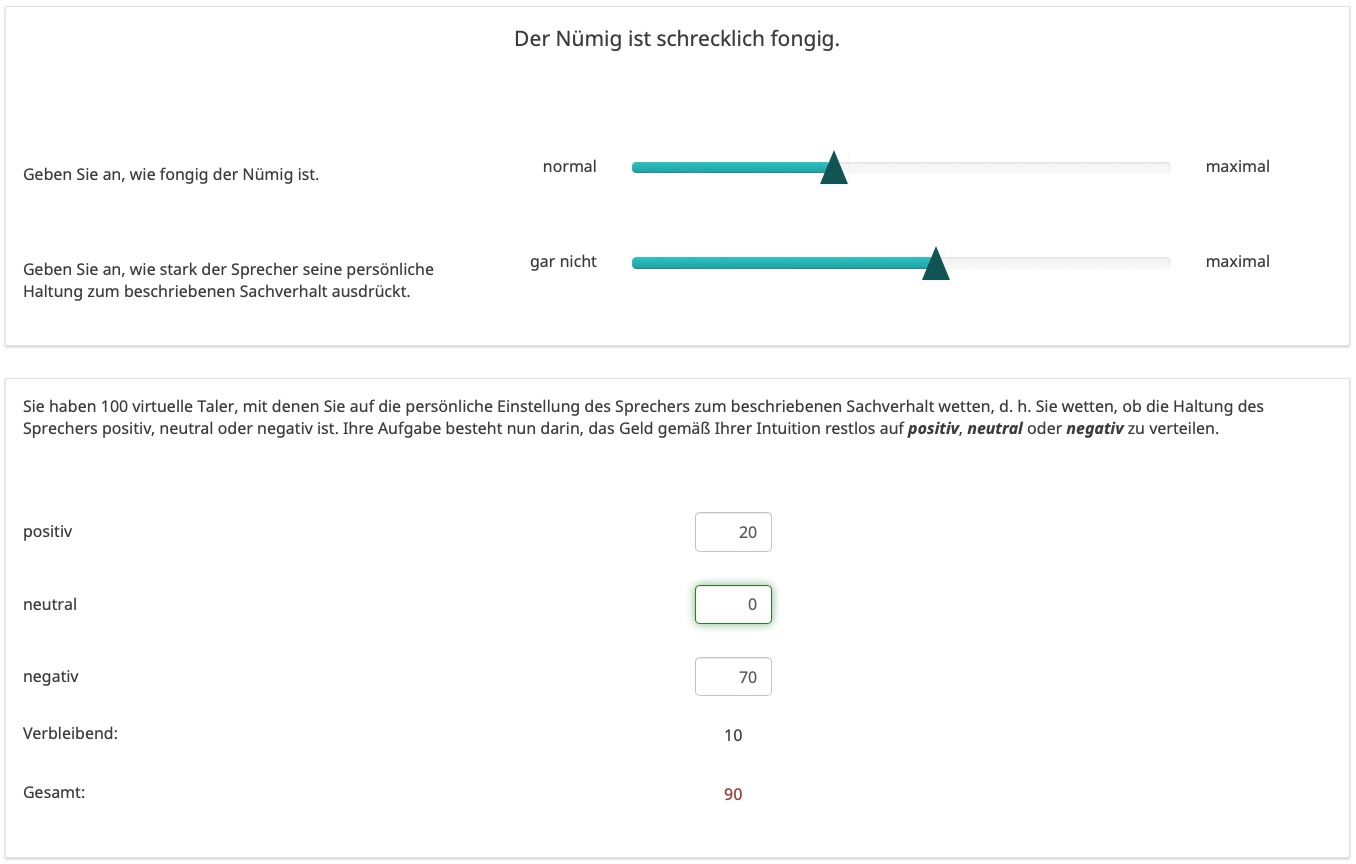
\includegraphics[angle=-90, width=0.67\textwidth]{Screen}
  \caption[Exemplarische Ansicht eines Items von Experiment 1] {Exemplarische Ansicht eines Items von Experiment 1.}
  \label{Screen1}
\end{figure}

\chapter{{Experimentelle Studie 1 -- Ratings der Intensivierer}} \label{Rat1}
\vspace*{-\baselineskip}
\begin{figure}[h!]
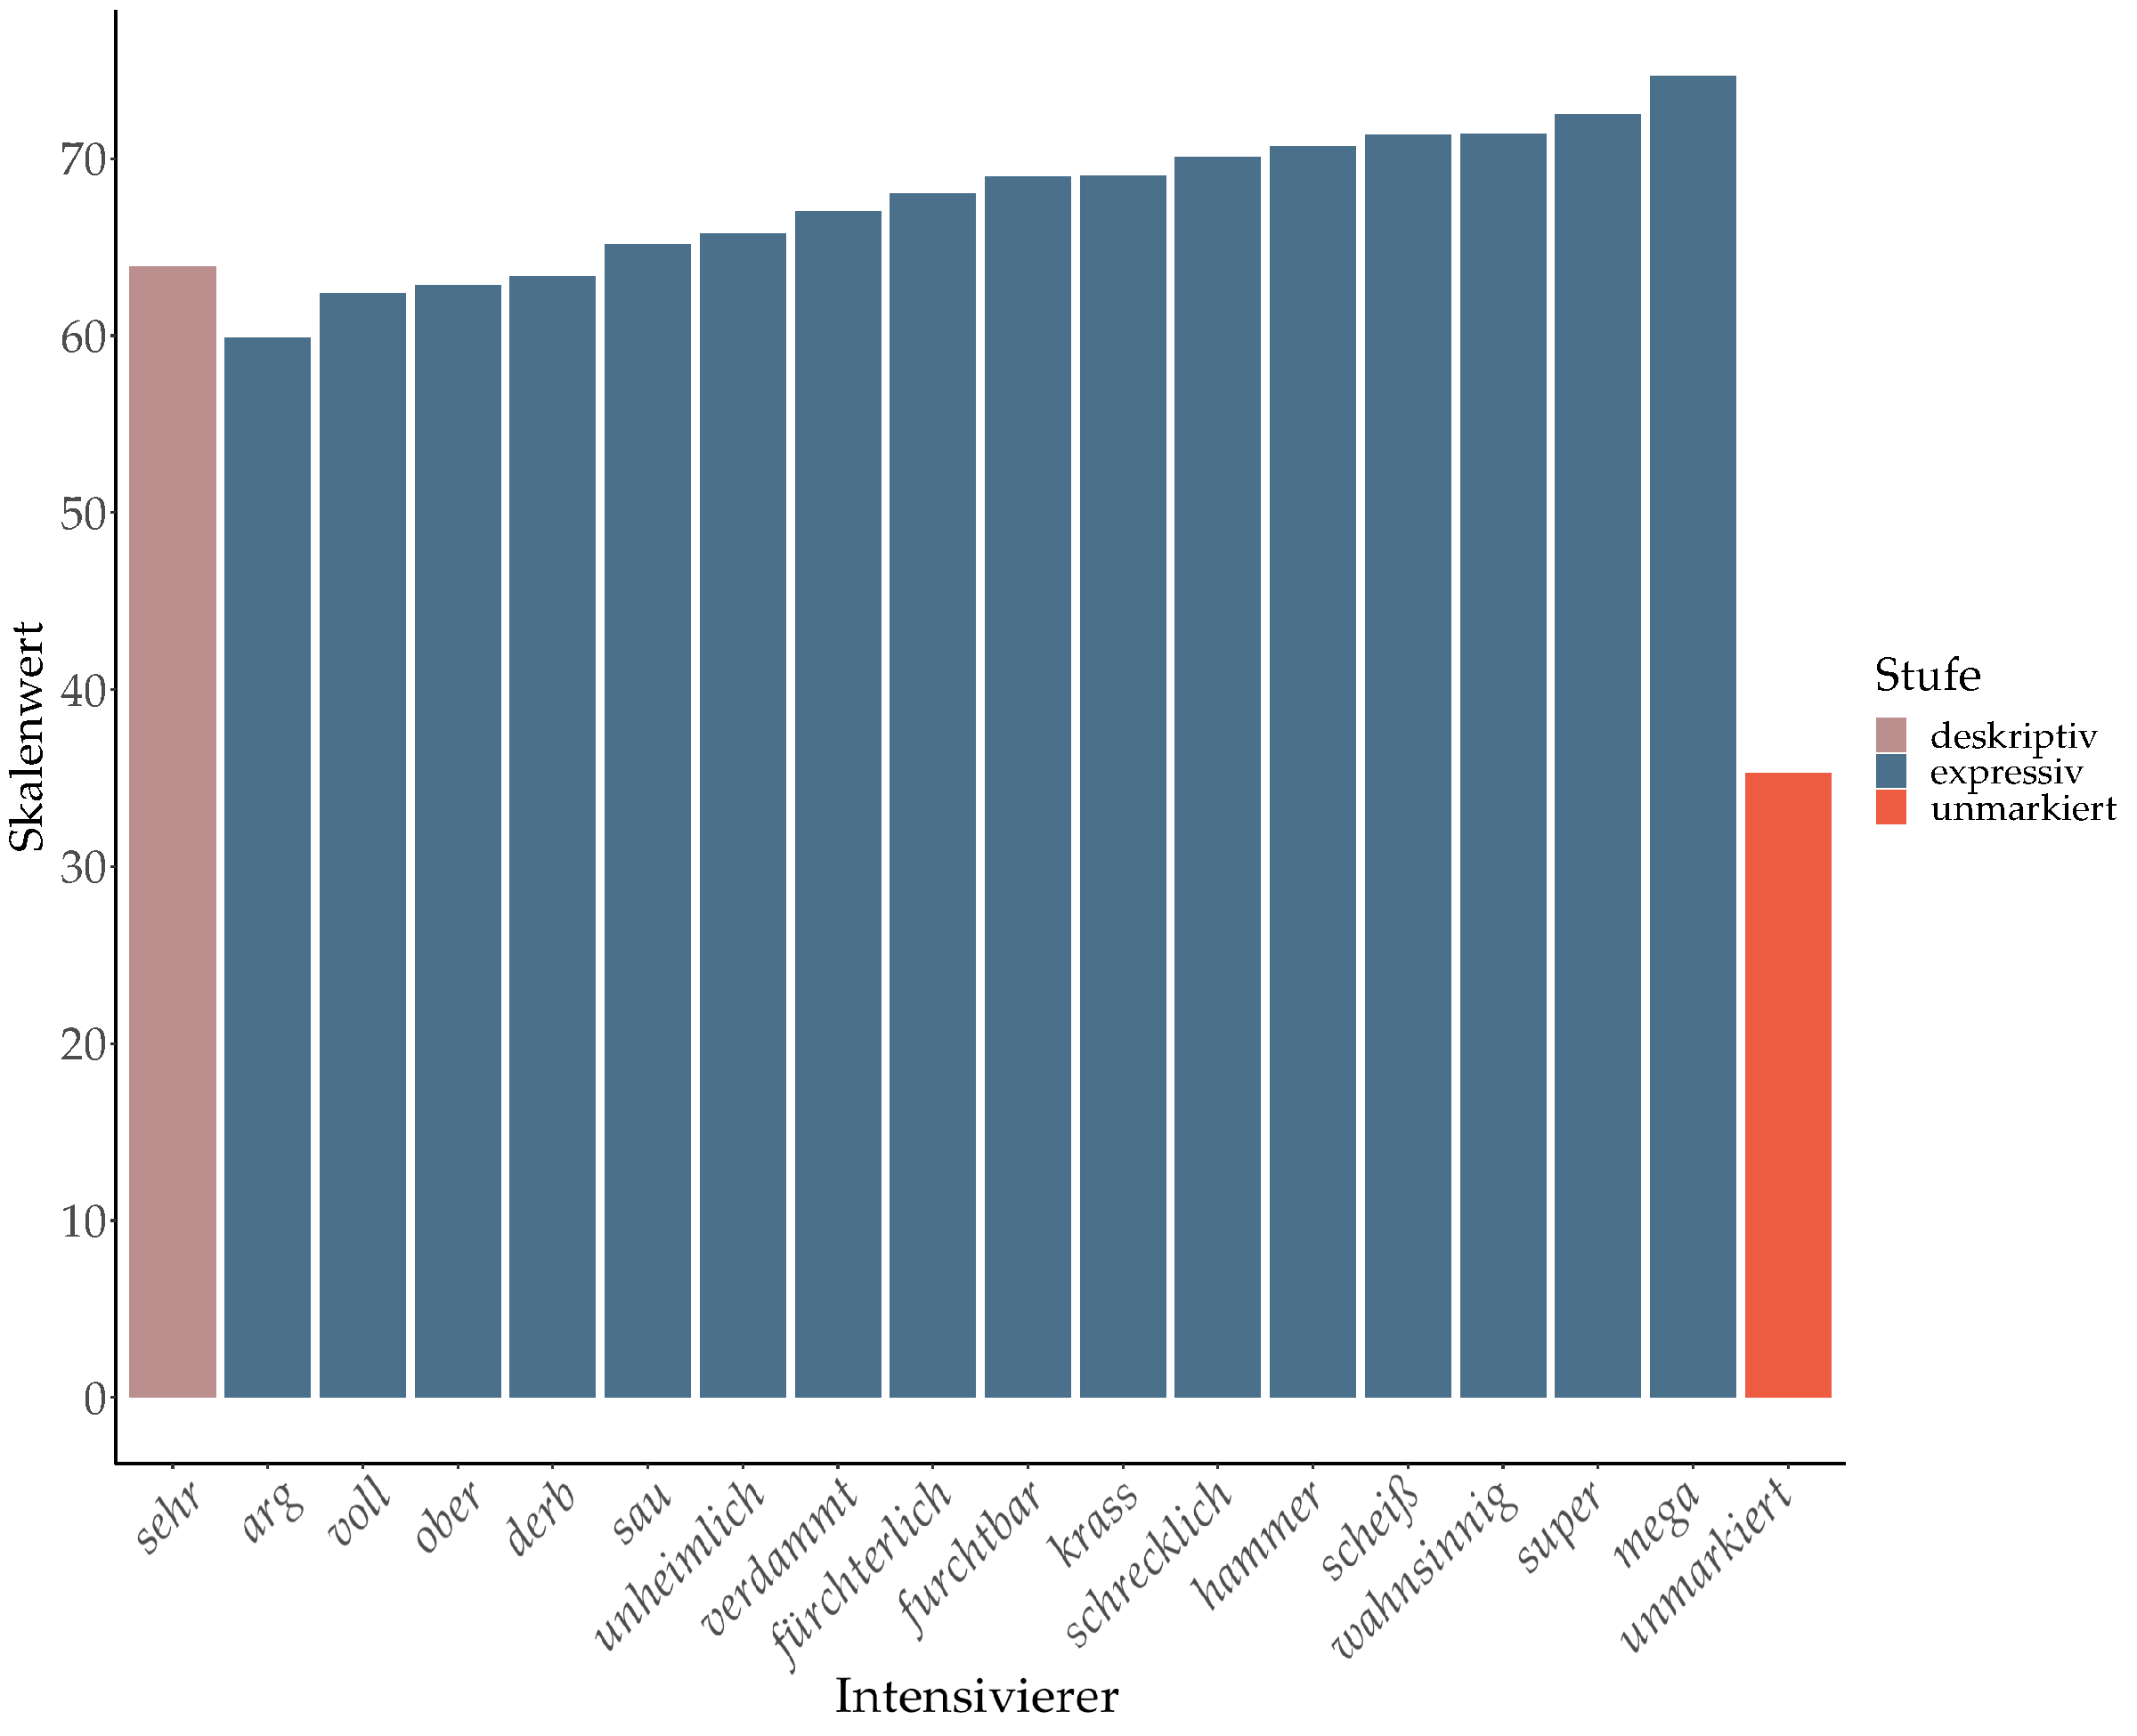
\includegraphics[angle=-90, width=0.8\textwidth]{Skalar7_neu}
\caption[Säulendiagramm zu den einzelnen Intensivierern bei Aufgabe I von Experiment 1]{Säulendiagramm zu den einzelnen Intensivierern bei Aufgabe I -- Skalarität ({x-Achse =} Intensivierer, y-Achse = Skalenwert).}
\label{Skalar7}
\end{figure}

\chapter{{Experimentelle Studie 1 -- Ratings der Pseudowörter}}  \label{Pseu1}
\begin{table}
\begin{tabularx}{.8\textwidth}{lYY}
\lsptoprule
   \multicolumn{3}{c}{\textbf{Aufgabe I Skalarität}}   \\
   \midrule
{Pseudonomen -- Pseudoadjektiv} & Skalenwert  &   \textit{SD} \\
\midrule
 \rowcolor[gray]{.90}  \textit{Der Gedalst -- wübig} &   62,55   & 25,0  \\
                        \textit{Das Zülugs -- wosplich} &  62,76    & 24,0 \\
  \rowcolor[gray]{.90}  \textit{Das Genavs -- laukrig} &  63,39    & 24,3 \\
                        \textit{Das Zeseet -- bühllich} &   63,76    & 24,4  \\
    \rowcolor[gray]{.90} \textit{Der Cobe -- speiglich} &  63,79    & 24,1 \\
                        \textit{Der Wonger -- zänsig} &  64,25    & 24,8  \\
    \rowcolor[gray]{.90} \textit{Der Zegeff -- ralklich} &  64,81    & 25,4   \\
                        \textit{Der Zotzer -- galklich} &  65,45    & 21,7  \\
   \rowcolor[gray]{.90}   \textit{Die Itne -- schühnlich} &  65,48  & 23,1   \\
                          \textit{Das Tusern -- zarwig} &  65,54    & 24,5  \\
   \rowcolor[gray]{.90}   \textit{Der Pulpart -- röngig} & 65,55   & 24,4  \\
                           \textit{Der Nümig -- fongig} &  65,94    & 25,0  \\
    \rowcolor[gray]{.90}     \textit{Der Conen -- waumlich} &  66,08 & 23,7   \\
                             \textit{Der Jordruck -- kieflich} &  67,02    & 23,8  \\
      \rowcolor[gray]{.90}  \textit{Das Hensuln -- ontig} &  67,57  & 22,1  \\
                            \textit{Die Itse -- rümmig} &  69,05   & 21,6  \\
     \rowcolor[gray]{.90}   \textit{Der Darster -- ormig} &  69,63    & 22,8  \\
                          \textit{Das Zafche -- göcktig} &  69,69    & 22,0  \\
\lspbottomrule
\end{tabularx}
\caption[Gemittelte Skalenwerte der Pseudowörter bei {Aufgabe I} von Experiment 1]{Gemittelte Skalenwerte und Standardabweichungen der Kombination aus Pseudonomen und Pseudoadjektiv bei Aufgabe I -- Skalarität (angeordnet nach ansteigendem Skalenwert).}
\label{Pseudos1}
\end{table}

\chapter{{Experimentelle Studie 1 -- Ratings der Pseudowörter}}  \label{Happy0}
\vspace{-\baselineskip}
\begin{figure}[h!]
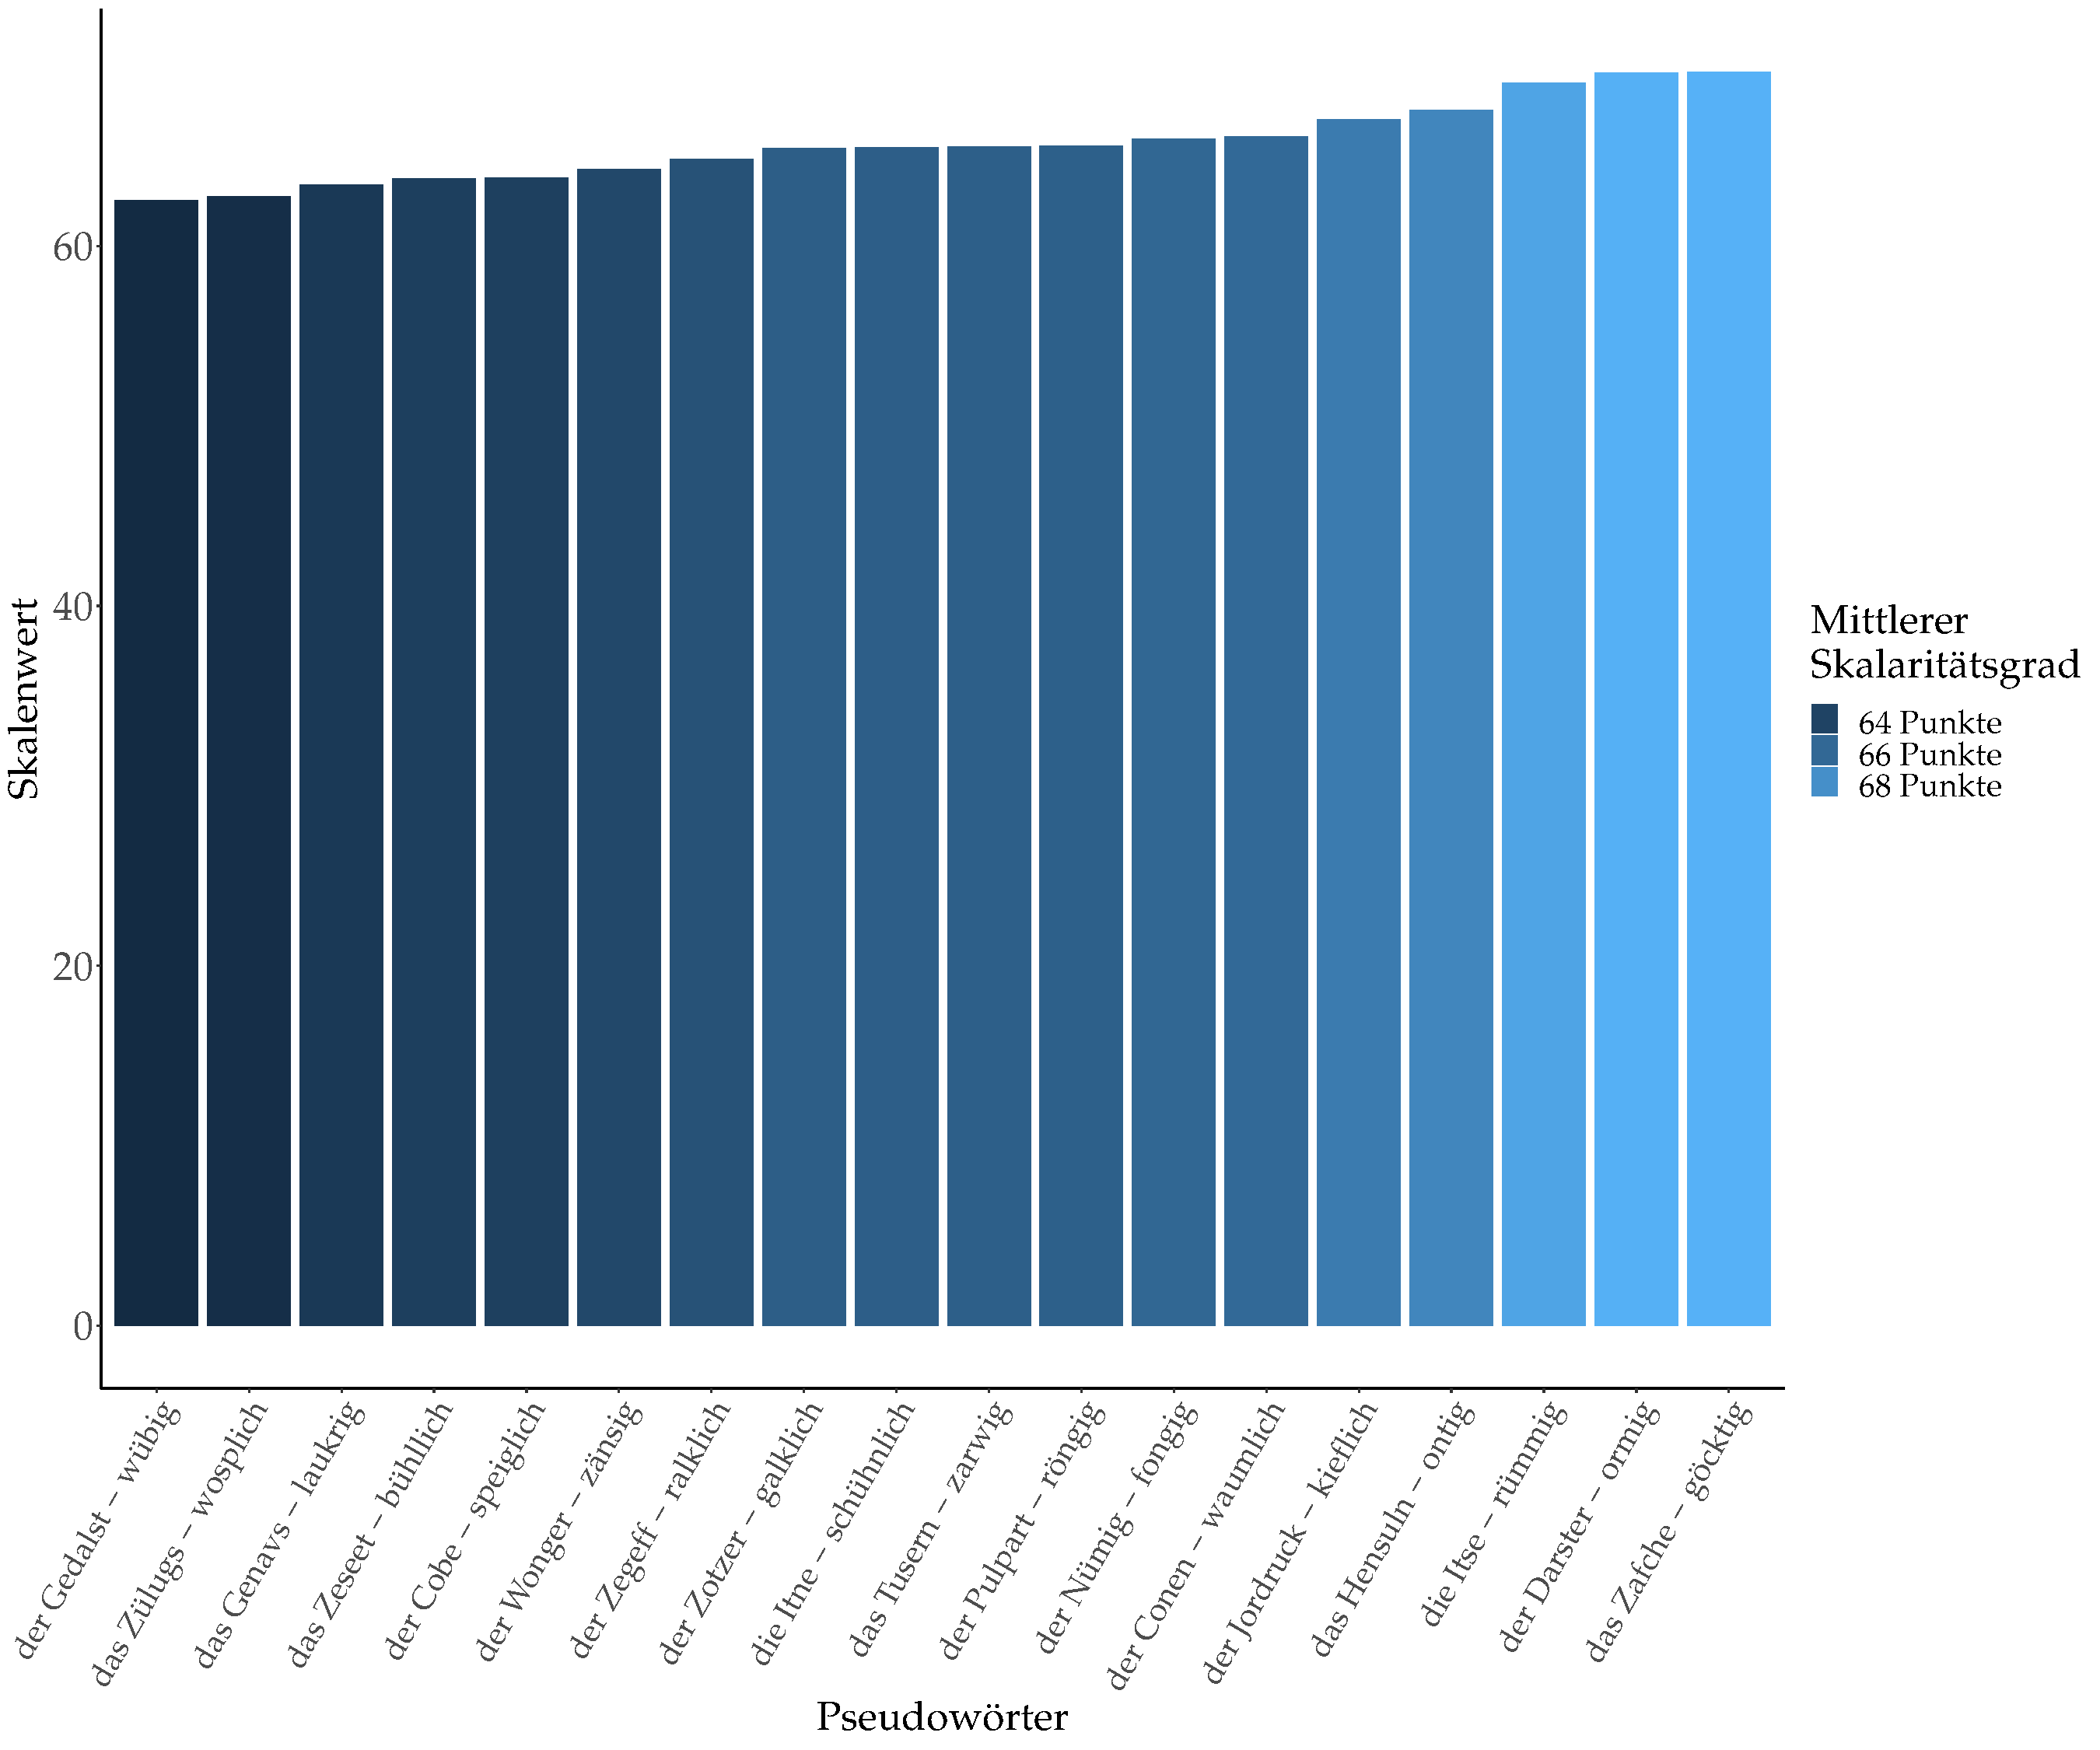
\includegraphics[angle=-90, width=0.8\textwidth]{Happy1}
\caption[Säulendiagramm zu den einzelnen Pseudowörtern bei Aufgabe I von Experiment 1]{Säulendiagramm zu den einzelnen Pseudowort-Kombinationen bei Aufgabe I -- Skalarität ({x-Achse =} Pseudowörter, y-Achse = Skalenwert).}
\label{Happy3}
\end{figure}

\chapter{{Experimentelle Studie 1 -- Ratings der Intensivierer}}  \label{Rat2}
\vspace{-\baselineskip}
\begin{figure}[h!]
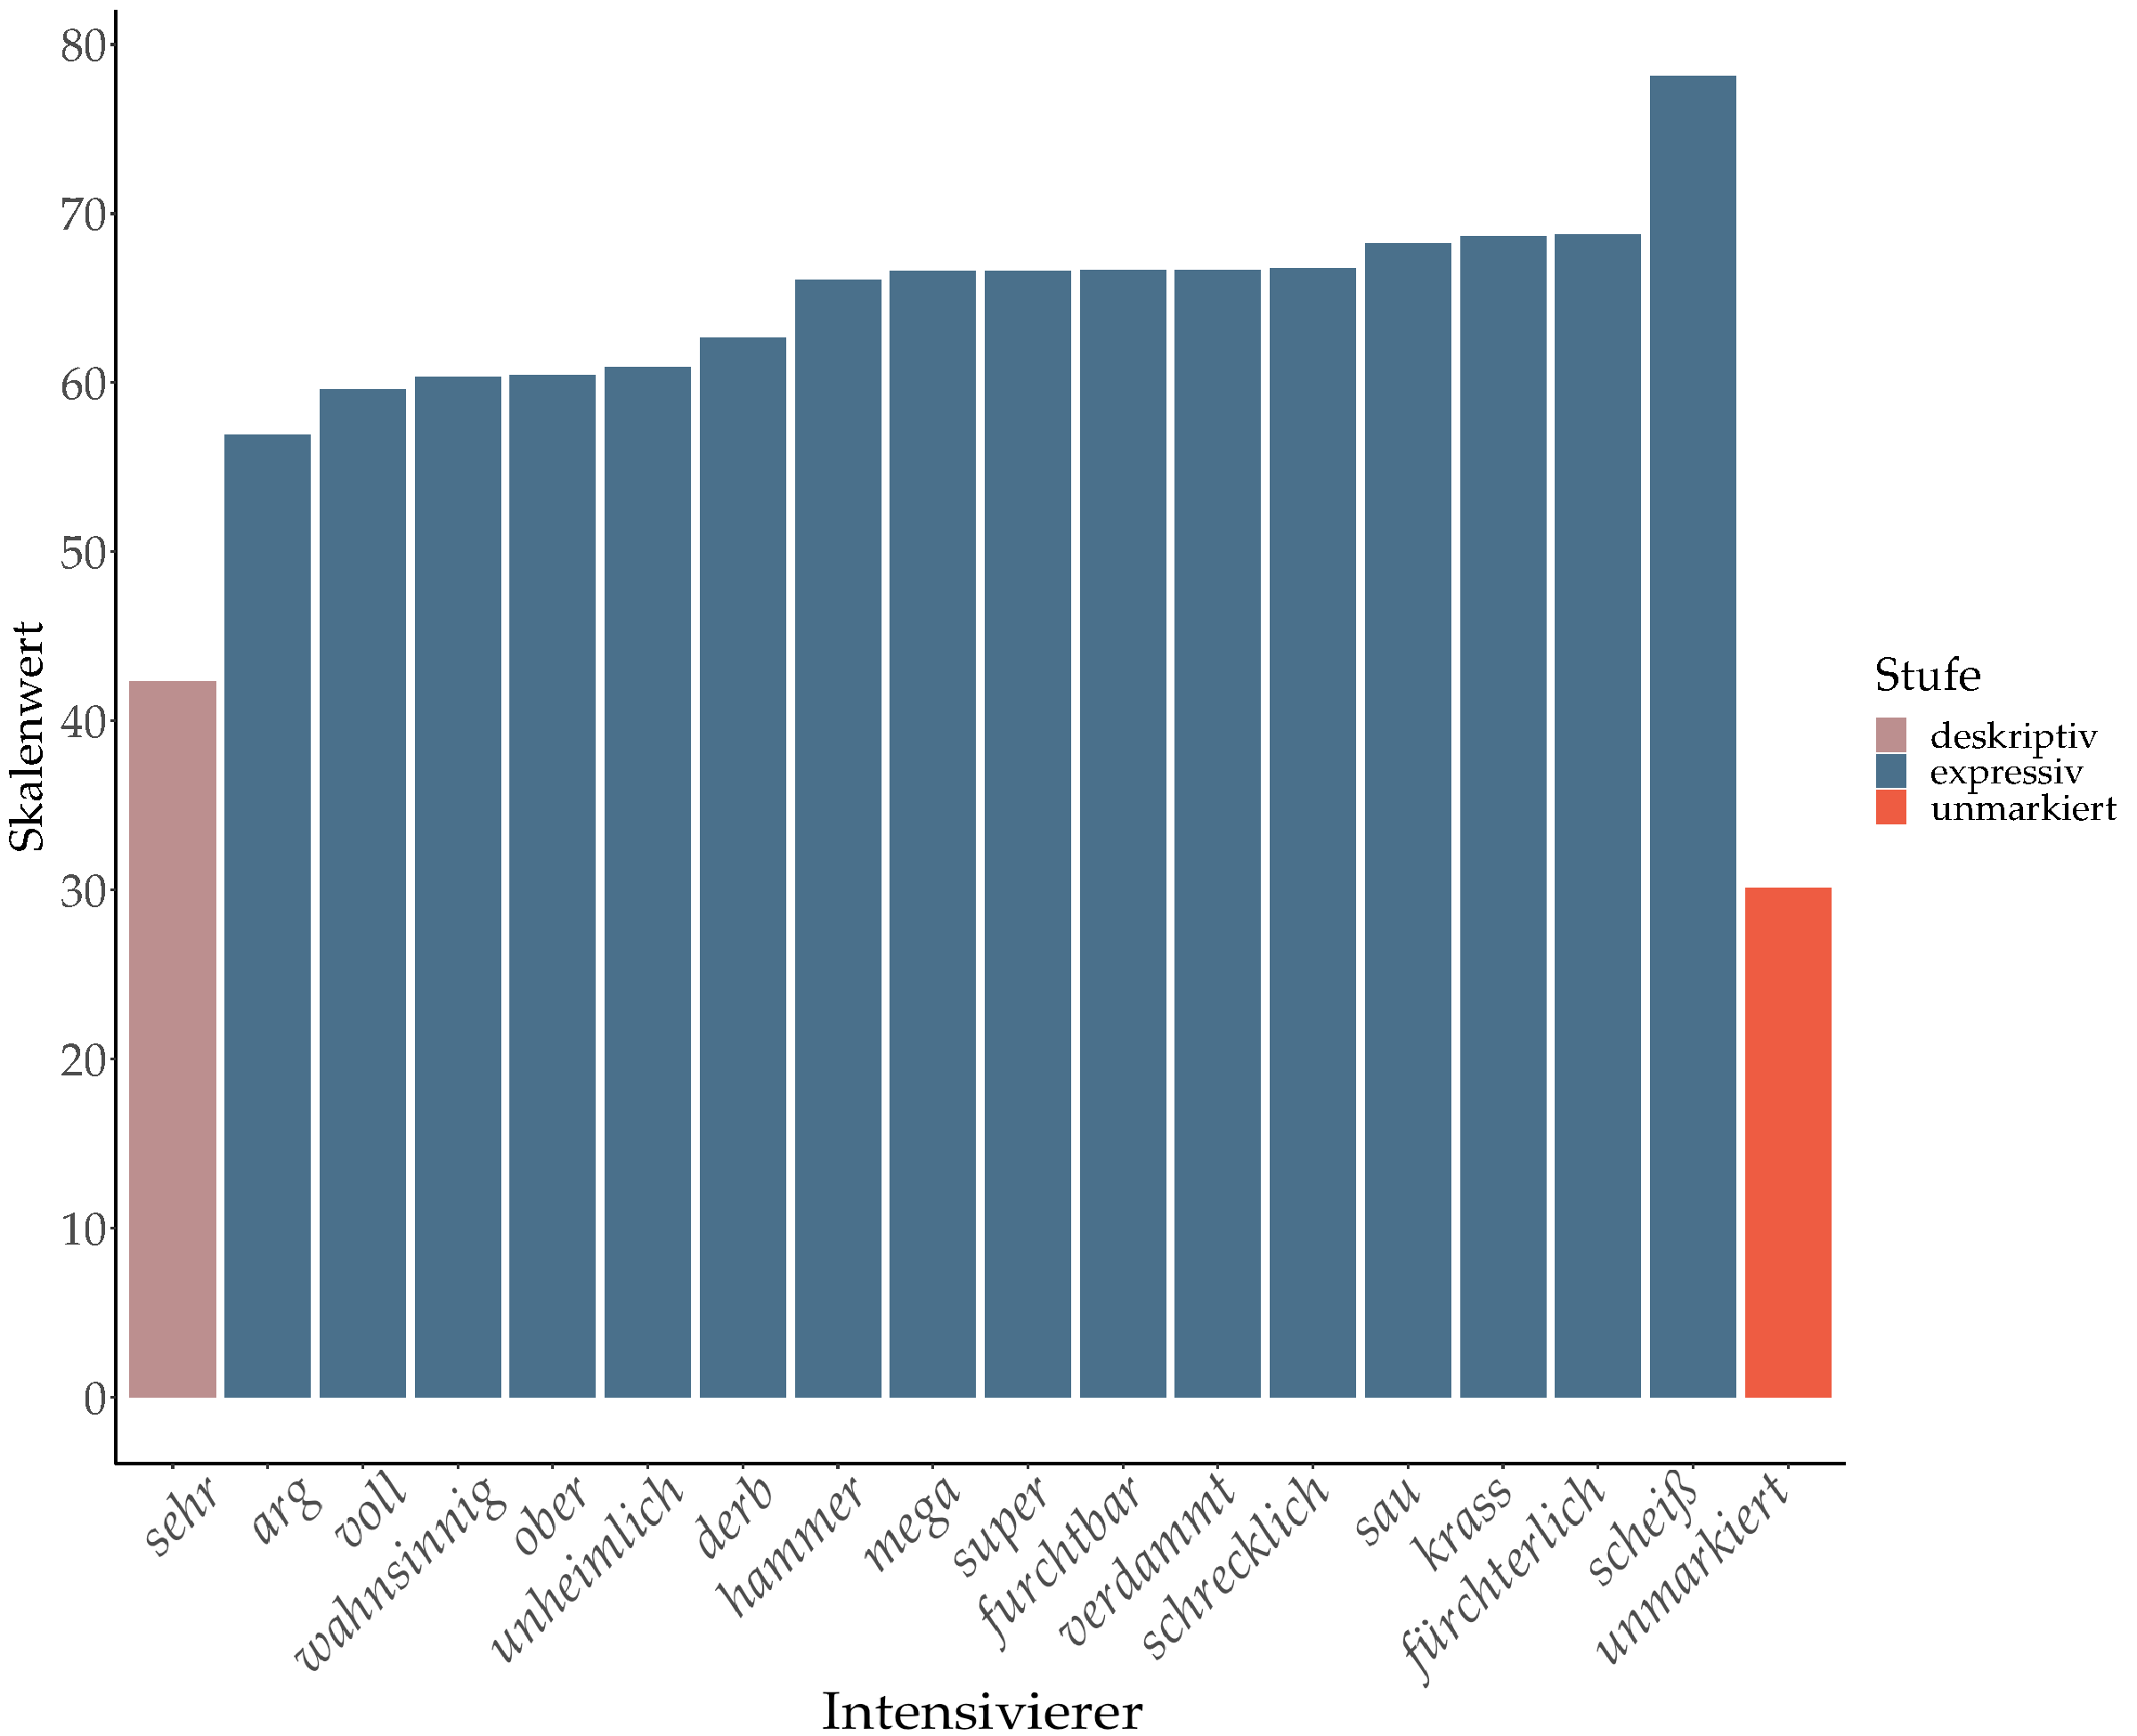
\includegraphics[angle=-90, width=0.8\textwidth]{Expressiv7_neu}
\caption[Säulendiagramm zu den einzelnen Intensivierern bei Aufgabe II von Experiment 1]{Säulendiagramm zu den einzelnen Intensivierern bei Aufgabe II -- Sprechereinstellung ({x-Achse =} Intensivierer, y-Achse = Skalenwert).}
\label{Expressiv7}
\end{figure}

\chapter{{Experimentelle Studie 1 -- Ratings der Pseudowörter}}   \label{Pseu2}

\begin{table}
\begin{tabularx}{.8\textwidth}{lYY}
\lsptoprule
   \multicolumn{3}{c}{\textbf{Aufgabe II Sprechereinstellung}}   \\
   \midrule
{Pseudonomen -- Pseudoadjektiv} & Skalenwert  &   \textit{SD} \\
\midrule
 \rowcolor[gray]{.90}     \textit{Der Cobe -- speiglich} &  58,75   & 27,6  \\
                        \textit{Der Wonger -- zänsig} &  59,12    & 25,4  \\
  \rowcolor[gray]{.90}    \textit{Das Tusern -- zarwig} &  60,11   & 27,5   \\
                        \textit{Der Gedalst -- wübig} &   60,25   & 27,1  \\
    \rowcolor[gray]{.90}    \textit{Der Jordruck -- kieflich} &  60,81  & 27,8  \\
                        \textit{Der Nümig -- fongig} &  60,84    & 26,7  \\
 \rowcolor[gray]{.90}     \textit{Das Zülugs -- wosplich} &  61,16  & 27,6    \\
                      \textit{Der Pulpart -- röngig} & 61,37    & 24,7  \\
    \rowcolor[gray]{.90}     \textit{Der Conen -- waumlich} &  61,39    & 26,8  \\
                        \textit{Das Zeseet -- bühllich} &   61,96    & 25,9  \\
    \rowcolor[gray]{.90}   \textit{Der Darster -- ormig} &  62,66   & 28,6  \\
                        \textit{Der Zotzer -- galklich} &  62,66    & 25,4  \\
   \rowcolor[gray]{.90}    \textit{Die Itse -- rümmig} &  62,76  & 26,2  \\
                      \textit{Das Zafche -- göcktig} &  63,88    & 25,3  \\
    \rowcolor[gray]{.90}   \textit{Das Hensuln -- ontig} &  64,15    & 29,6 \\
                        \textit{Das Genavs -- laukrig} &  64,48   & 27,9   \\
   \rowcolor[gray]{.90}   \textit{Der Zegeff -- ralklich} &  64,69   & 25,8    \\
                        \textit{Die Itne -- schühnlich} &  65,34     & 24,3  \\
\lspbottomrule
\end{tabularx}
\caption[Gemittelte Skalenwerte der Pseudowörter bei {Aufgabe II} von Experiment 1]{Gemittelte Skalenwerte und Standardabweichungen der Kombination aus Pseudonomen und Pseudoadjektiv bei Aufgabe II -- Sprechereinstellung (angeordnet nach ansteigendem Skalenwert).}
\label{Pseudos2}
\end{table}

\chapter{{Experimentelle Studie 1 - Ratings der Pseudowörter}}  \label{Happy4}
\vspace*{-\baselineskip}

\begin{figure}[h!]
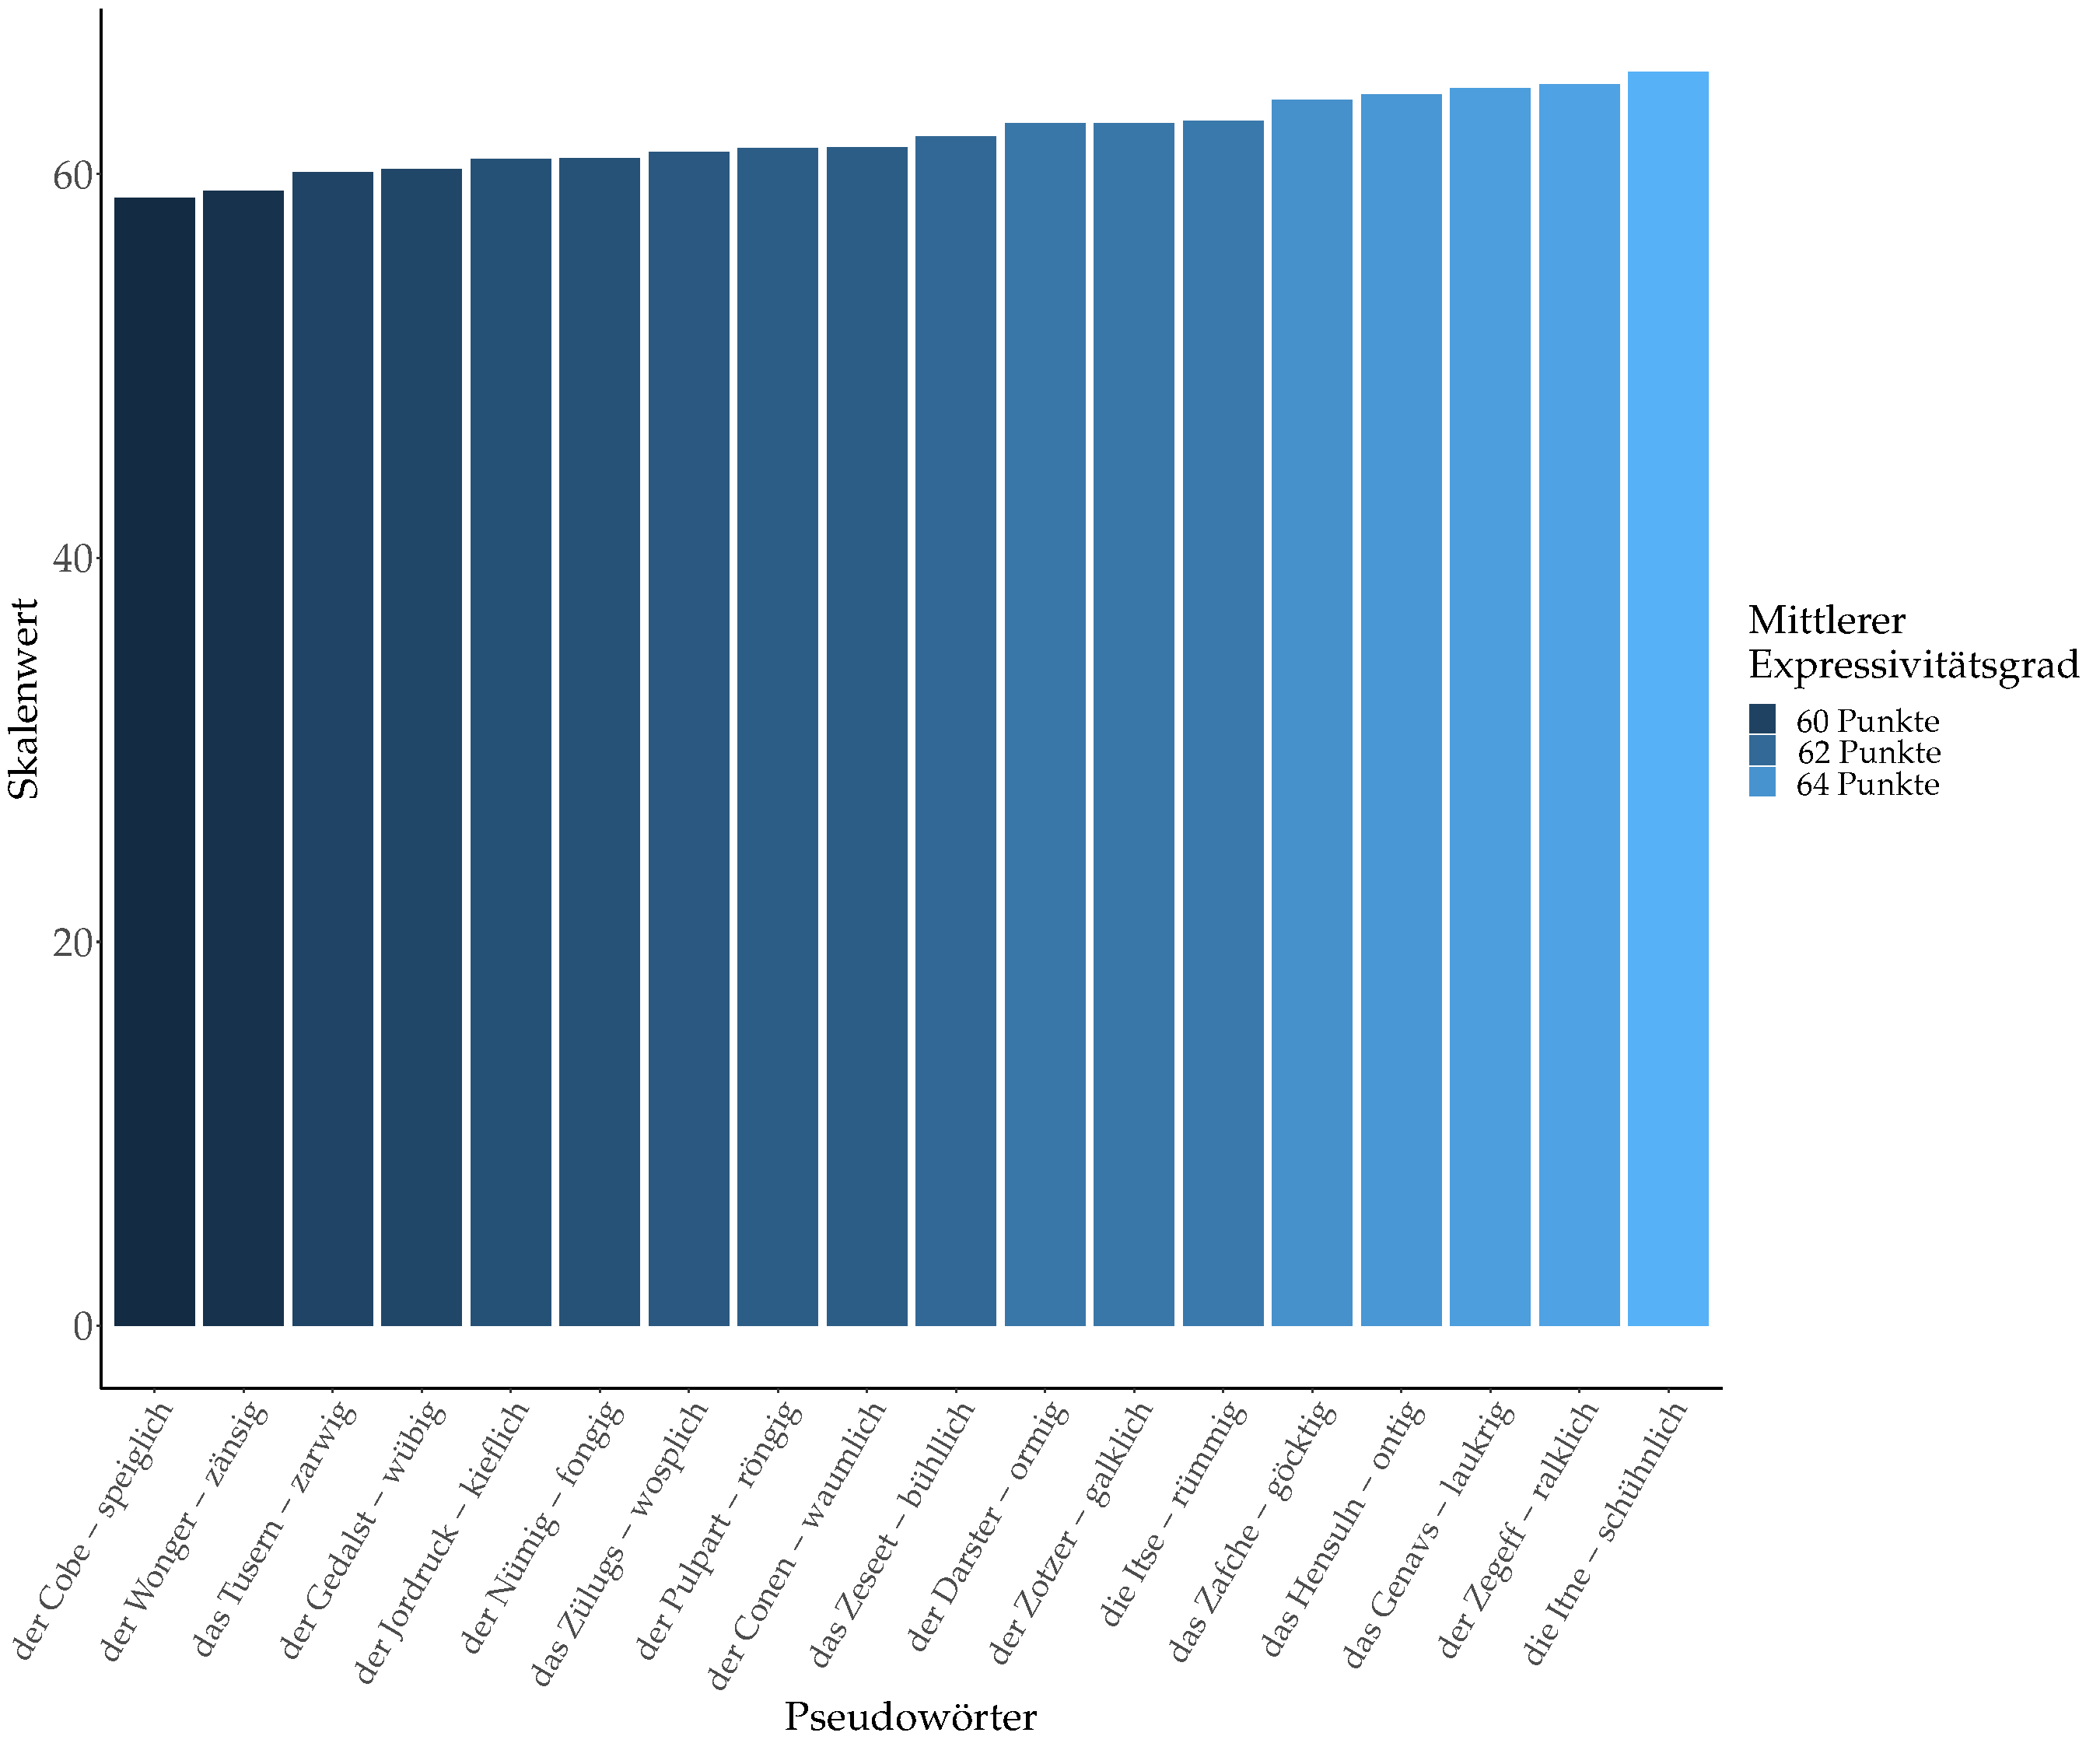
\includegraphics[angle=-90, width=0.8\textwidth]{Happy3}
\caption[Säulendiagramm zu den einzelnen Pseudowörtern bei Aufgabe II von Experiment 1]{Säulendiagramm zu den einzelnen Pseudowort-Konbinationen bei Aufgabe II -- Sprechereinstellung ({x-Achse =} Pseudowörter, {y-Achse =} Skalenwert).}
\label{Happy5}
\end{figure}

\chapter{{Experimentelle Studie 1 -- Ratings der Pseudowörter}}  \label{Pseu3}

\begin{table}
\begin{tabularx}{\textwidth} {lYYYYYY}

\lsptoprule
 & \multicolumn{6}{c}{\textbf{Aufgabe III Pseudowörter}}\\
 \midrule
 & \multicolumn{6}{c}{\textbf{Einstellungspolarität}}  \\
  &\multicolumn{2}{c}{\textsc{positiv}} & \multicolumn{2}{c}{\textsc{neutral}} & \multicolumn{2}{c}{\textsc{negativ}} \\
 \cmidrule(lr){2-3}\cmidrule(lr){4-5}\cmidrule(lr){6-7}
  & Taler& \textit{SD}  & Taler& \textit{SD}  & Taler& \textit{SD}   \\
\midrule
 \rowcolor[gray]{.90}   \textit{Der Conen -- waumlich} & 45,45& 32,3 &  24,37 & 23,9 & 30,18  & 29,7\\
                  \textit{Der Darster -- ormig} & 30,06 & 28,4 & 34,78& 30,9  & 35,16 & 33,6    \\
 \rowcolor[gray]{.90}    \textit{Die Itne -- schühnlich} & 33,87& 29,0 & 30,73  & 29,4 & 35,40 & 31,0  \\
                        \textit{Das Genavs -- laukrig} & 31,12& 28,3 & 33,07& 28,1 & 35,81  & 33,8     \\
 \rowcolor[gray]{.90}     \textit{Das Zafche -- göcktig} & 37,23& 32,4 & 26,46  & 28,8 &  36,31 & 34,1 \\
                            \textit{Der Nümig -- fongig} & 34,84& 30,1 & 28,79& 26,8  & 36,37& 29,4 \\
\rowcolor[gray]{.90}    \textit{Das Tusern -- zarwig} & 29,03& 26,1  & 33,64 & 29,6  &  37,33  & 32,8 \\
                        \textit{Der Jordruck -- kieflich} & 29,15  & 29,2&  32,48& 31,0 &  38,37  & 33,4 \\
  \rowcolor[gray]{.90}    \textit{Die Itse -- rümmig} & 30,33  & 27,7 & 30,94 & 27,4  &  38,73 & 32,9  \\
                        \textit{Der Wonger -- zänsig} & 29,31 & 28,6  &  31,93 & 27,8&  38,76 & 32,5  \\
  \rowcolor[gray]{.90}    \textit{Das Zülugs -- wosplich} & 30,79  & 30,0 & 30,43 & 28,5   & 38,78 & 28,7\\
                        \textit{Der Zegeff -- ralklich} & 28,14 & 27,6 &  32,16 & 29,7 &  39,70  & 32,3\\
 \rowcolor[gray]{.90}  \textit{Das Hensuln -- ontig} & 31,88   & 30,5&  28,13 & 26,0 & 39,99 & 32,8 \\
                        \textit{Der Cobe -- speiglich} & 29,30& 29,1 &  30,45   & 29,8 & 40,25& 35,0  \\
 \rowcolor[gray]{.90}  \textit{Der Gedalst -- wübig} & 27,79  & 29,9 & 31,82 & 29,0  & 40,39& 31,6 \\
                          \textit{Das Zeseet -- bühllich} & 30,94 & 30,1 & 28,19  & 26,4 &  40,87  & 31,6 \\
 \rowcolor[gray]{.90}    \textit{Der Zotzer -- galklich} & 28,16 & 28,4  &  30,30 & 29,8&  41,54  & 32,0 \\
                        \textit{Der Pulpart -- röngig} & 28,01  & 25,7&  27,18 & 26,0 &  44,81  & 29,7\\
\bottomrule
\end{tabularx}
\caption[Mittel der gesetzten Taler der Pseudowörter bei {Aufgabe III} von Experiment 1]{Mittel der gesetzten Taler und Standardabweichungen der Kombination aus Pseudonomen und Pseudoadjektiv bei Aufgabe III -- Einstellungspolarität (Talersumme je Wortpaar = 100; angeordnet nach ansteigendem negativen Skalenwert).}
\label{Pseudos3}
\end{table}

\chapter{{Experimentelle Studie 1 -- Regressionsmodelle}} \label{Regr1}



\section{Aufgabe I -- Skalarität}

\subsection{{Tabelle \ref{LinReg0001}}}
\ea
Formel des vollen Modells zu Aufgabe I -- Skalarität (mit `Expressiv' als Referenzlevel):\smallskip

$ lmer(\text{Skalenwert}\sim(\text{Expr vs. Desk}+\text{Expr vs. Unm)} * \text{Position} + (1 + (\text{Expr vs. Desk} + \text{Expr vs. Unm}) * \text{Position}|\text{Versuchspers.}) + (1|\text{Pseudow.})) $
\z



\ea
Formel des finalen Modells zu Aufgabe I -- Skalarität (mit `Expressiv' als Referenzlevel):\smallskip

$ lmer(\text{Skalenwert}\sim\text{Expr vs. Desk}+\text{Expr vs. Unm} + \text{Position} + (1 + (\text{Expr vs. Desk} + \text{Expr vs. Unm}) * \text{Position}|\text{Versuchspers.}) + (1|\text{Pseudow.})) $
\z


\subsection{{Tabelle \ref{LinReg0010}}}
\ea
Formel des vollen Modells zu Aufgabe I -- Skalarität (mit `Unmarkiert' als Referenzlevel):\smallskip

$ lmer(\text{Skalenwert} \sim (\text{Unm vs. Desk} + \text{Unm vs. Expr)} * \text{Position} + (1 + (\text{Unm vs. Desk} + \text{Unm vs. Expr)} * \text{Position|Versuchspers.}) + (1|\text{Pseudow.})) $
\z

\ea
Formel des finalen Modells zu Aufgabe I -- Skalarität (mit `Unmarkiert' als Referenzlevel):\smallskip

$ lmer(\text{Skalenwert} \sim \text{Unm vs. Desk} + \text{Unm vs. Expr} + \text{Position} + (1 + (\text{Unm vs. Desk} + \text{Unm vs. Expr}) * \text{Position|Versuchspers.}) + (1|\text{Pseudow.})) $
\z

\subsection{{Tabelle \ref{LinRea0100}}}
\ea
Formel des vollen Modells zu Aufgabe I -- Skalarität

(Einfluss von Frequenz mit `Hoch' als Referenzlevel, Persistenz mit `Alt' als Referenzlevel):\smallskip

$ lmer(\text{Skalenwert} \sim (\text{Frequenz + Persistenz}) * \text{Position} + (1 +(\text{Frequenz + Persistenz}) * \text{Position|Versuchspers.}) + (1|\text{Pseudow.})) $
\z

\ea
Formel des finalen Modells zu Aufgabe I -- Skalarität

(Einfluss von Frequenz mit `Hoch' als Referenzlevel, Persistenz mit `Alt' als Referenzlevel):\smallskip

$ lmer(\text{Skalenwert} \sim (\text{Frequenz + Persistenz}) * \text{Position} - \text{Frequenz : Position - Persistenz : Position} + (1 + (\text{Frequenz + Persistenz}) * \text{Position|Versuchspers.}) + (1|\text{Pseudow.})) $
\z



\section{Aufgabe II -- Sprechereinstellung}

\subsection{{Tabelle \ref{LinReg0002}}}
\ea
Formel des vollen Modells zu Aufgabe II -- Sprechereinstellung (mit `Expressiv' als Referenzlevel):\smallskip

$ lmer(\text{Skalenwert} \sim (\text{Expr vs. Desk} + \text{Expr vs. Unm}) * \text{Position} + (1 + (\text{Expr vs. Desk} + \text{Expr vs. Unm}) * \text{Position|Versuchspers.}) + (1|\text{Pseudow.}))$
\z

\ea
Formel des finalen Modells zu Aufgabe II -- Sprechereinstellung (mit `Expressiv' als Referenzlevel):\smallskip

$ lmer(\text{Skalenwert} \sim \text{Expr vs. Desk} + \text{Expr vs. Unm} + (1 + (\text{Expr vs. Desk} + \text{Expr vs. Unm}) * \text{Position|Versuchspers.}) + (1|\text{Pseudow.})) $
\z


\subsection{{Tabelle \ref{LinReg0020}}}

\ea
Formel des vollen Modells zu Aufgabe II -- Sprechereinstellung (mit `Unmarkiert' als Referenzlevel):\smallskip

$ lmer(\text{Skalenwert} \sim (\text{Unm vs. Desk} + \text{Unm vs. Expr}) * \text{Position} + (1 + (\text{Unm vs. Desk} + \text{Unm vs. Expr}) * \text{Position|Versuchspers.}) + (1|\text{Pseudow.})) $
\z

\ea
Formel des finalen Modells zu Aufgabe II -- Sprechereinstellung (mit `Unmarkiert' als Referenzlevel):\smallskip

$ lmer(\text{Skalenwert} \sim \text{Unm vs. Desk} + \text{Unm vs. Expr} + (1 + (\text{Unm vs. Desk} + \text{Unm vs. Expr}) * \text{Position|Versuchspers.}) + (1|\text{Pseudow.})) $
\z

\subsection{{Tabelle \ref{LinRegzaz0}}}
\ea
Formel des vollen Modells zu Aufgabe II -- Sprechereinstellung

(Einfluss von Frequenz mit `Hoch' als Referenzlevel, Persistenz mit `Alt' als Referenzlevel):
\smallskip

$ lmer(\text{Skalenwert} \sim (\text{Frequenz + Persistenz}) * \text{Position}) + (1 +(\text{Frequenz + Persistenz}) * \text{Position|Versuchspers.}) + (1|\text{Pseudow.})) $
\z

\ea Formel des finalen Modells zu Aufgabe II - Sprechereinstellung 

(Einfluss von Frequenz mit Hoch' als Referenzlevel, Persistenz mit Alt' als Referenzlevel):
\smallskip


$ lmer(\text{Skalenwert} \sim (\text{Frequenz + Persistenz}) * \text{Position}) - \text{Position} - \linebreak \text{Persistenz} - \text{Frequenz} : \text{Persistenz} - \text{Persistenz} : \text{Position} - \text{Frequenz} : \text{Position} + (1 + (\text{Frequenz} + \text{Persistenz}) * \text{Position}|\text{Versuchspers.}) + (1|\text{Pseudow.}) $
\z


\subsection{{Tabelle \ref{LM01}}}
\ea Formel des linearen Modells zum Einfluss von Sprechereinstellung auf Skalarität:
\smallskip


$ lm(\text{Skalarität} \sim \text{Sprechereinstellung}) $
\z


\section{Aufgabe III -- Einstellungspolarität}



\subsection{{Tabelle \ref{LinReg0004}}}
\ea

Formel des vollen Modells zu Aufgabe III -- Einstellungspolarität (mit `Neutral' als Referenzlevel):
\smallskip


$ lmer(\text{Neutral} \sim (\text{Sprechereinstellung + Skalarität}) * \text{Position} + (1 + (\text{Sprechereinstellung + Skalarität}) * \text{Position|Versuchspers.}) +  (1|\text{Pseudow.})) $
\z

\ea
Formel des finalen Modells zu Aufgabe III -- Einstellungspolarität (mit `Neutral' als Referenzlevel):
\smallskip


$lmer(\text{Neutral} \sim (\text{Sprechereinstellung + Skalarität}) * \text{Position} - \text{Sprechereinstellung : Skalarität} - \text{Sprechereinstellung : Position} - \text{Skalarität : Position} + (1 + (\text{Sprechereinstellung + Skalarität}) * \text{Position|Versuchspers.}) + (1|\text{Pseudow.})) $
\z

\chapter{{Experimentelle Studie 2a -- Ratings der Adjektive}}   \label{Aja1}
\begin{table}

\begin{tabularx}{\textwidth}{l rY rY rY}
\lsptoprule
  \multicolumn{7}{c}{\textbf{Experiment 2a} \textbf{Skalarität}}  \\
  \midrule
 & \multicolumn{4}{c}{{Intensiviererklasse}}   \\
 \cmidrule{2-5}
{Adjektiv} &  deskriptiv &   \textit{SD} & expressiv &\textit{SD} &  {Mittelwert} &  \textit{SD}\\
\midrule
 \rowcolor[gray]{.90} \textit{breit} & 55,87& 23,5 & 60,25& 24,3 & 58,06 & 24,0 \\
                        \textit{lang} & 54,90  & 23,8& 62,03  & 22,5& 58,47 & 23,4 \\
  \rowcolor[gray]{.90} \textit{dick} & 57,27 & 23,4& 60,32  & 23,4 & 58,80 & 23,4 \\
                      \textit{groß} & 57,84 & 22,3 & 61,32 & 23,9  & 59,58 & 23,2 \\
  \rowcolor[gray]{.90}  \textit{hoch} & 58,33  & 23,8& 63,37 & 22,8 & 60,85 & 23,5  \\
                        \textit{alt} & 60,28 & 23,1 & 64,56 & 24,8  & 62,42& 24,0 \\
  \rowcolor[gray]{.90} \textit{heiß} & 62,79 & 23,6 & 66,82 & 25,1& 64,80 & 24,4 \\
\lspbottomrule

\end{tabularx}
\caption[Gemittelte Skalenwerte der Adjektive beider Intensiviererklassen von Experiment 2a]{Gemittelte Skalenwerte und Standardabweichungen der Adjektive beider Intensiviererklassen von Experiment 2a -- Skalarität (angeordnet nach ansteigendem Mittelwert).}
\label{Adj0}
\end{table}

\chapter{{Experimentelle Studie 2a -- Regressionsmodelle}}   \label{RegX}

\section{Experiment 2a -- Skalarität}

\subsection{{Tabelle \ref{LinReg01}}}

\ea
Formel des vollen Modells zu Experiment 2a -- Skalarität (mit `Deskriptiv' als Referenzlevel):
\smallskip


$ lmer(\text{Skalenwert} \sim (\text{Desk vs. Expr}) * \text{Position} + (1 + (\text{Desk vs. Expr}) * \text{Position|Versuchspers.}) + (1|\text{Adj.})) $
\z

\ea
Formel des finalen Modells zu Experiment 2a -- Skalarität (mit `Deskriptiv' als Referenzlevel):
\smallskip


$ lmer(\text{Skalenwert}\sim(\text{Desk vs. Expr}) * \text{Position} + (1 + (\text{Desk vs. Expr}) *\linebreak \text{Position}|\text{Versuchspers.}))$
\z


\subsection{{Tabelle \ref{Matrix_1_neu}}}

\ea
Formel der Paarvergleiche zu Experiment 2a -- Skalarität:
\smallskip


$ lmer(\text{Skalenwert} \sim \text{Intensivierer * Position} + (1|\text{Versuchspers.}) + (1|\text{Adj.})) $
\z


\chapter{{Experimentelle Studie 2b -- Ratings der Adjektive}}       \label{Aja3}
\begin{table}

\begin{tabularx}{\textwidth}{l rY rY rY}
\lsptoprule
  \multicolumn{7}{c}{\textbf{Experiment 2b Sprechereinstellung}}  \\
  \midrule
 & \multicolumn{4}{c}{{Intensiviererklasse}}   \\
 \cmidrule{2-5}
{Adjektiv} &  deskriptiv &   \textit{SD} & expressiv &\textit{SD} &  {Mittelwert} &  \textit{SD}\\
\midrule
 \rowcolor[gray]{.90} \textit{breit} & 44,75 & 26,3 & 55,13 & 29,7 & 49,94 & 28,5 \\
                      \textit{dick} & 44,60 & 27,4 & 61,25 & 29,1  & 52,93 & 29,4\\
 \rowcolor[gray]{.90} \textit{lang} & 48,54  & 28,4 & 60,68  & 28,6& 54,61  & 29,1\\
                      \textit{groß} & 51,54 & 27,6  & 59,59& 28,3 & 55,57  & 28,2\\
   \rowcolor[gray]{.90} \textit{alt} & 49,44  & 28,8& 62,24 & 28,3  & 55,84 & 29,2\\
                        \textit{hoch} & 50,43 & 28,0 & 61,81  & 27,2 & 56,12 & 28,2\\
  \rowcolor[gray]{.90} \textit{heiß} & 54,73  & 27,3& 62,32 & 28,0  & 58,52 & 27,8\\
\lspbottomrule

\end{tabularx}
\caption[Gemittelte Skalenwerte der Adjektive beider Intensiviererklassen von Experiment 2b]{Gemittelte Skalenwerte und Standardabweichungen der Adjektive beider Intensiviererklassen von Experiment 2b -- Sprechereinstellung (angeordnet nach ansteigendem Mittelwert).}
\label{Adj10}
\end{table}

\chapter{{Experimentelle Studie 2b -- Regressionsmodelle}}   \label{Aja2}


\section{Experiment 2b -- Sprechereinstellung}

\subsection{{Tabelle \ref{LinReg2}}}

\ea
Formel des vollen Modells zu Experiment 2b -- Sprechereinstellung

(mit `Deskriptiv' als Referenzlevel):\\
$ lmer(\text{Skalenwert} \sim (\text{Desk vs. Expr}) * \text{Position} + (1 + (\text{Desk vs. Expr}) * \text{Position|Versuchspers.}) + (1|\text{Adj.}))$
\z

\ea
Formel des finalen Modells zu Experiment 2b -- Sprechereinstellung\\
(mit `Deskriptiv' als Referenzlevel):
\smallskip


$ lmer(\text{Skalenwert} \sim (\text{Desk vs. Expr}) * \text{Position} - \text{Position} - \text{Desk vs. Expr} : \text{Position} + (1 + (\text{Desk vs. Expr}) * \text{Position}|\text{Versuchspers.})) $
\z
\subsection{{Tabelle \ref{LM02}}}

\ea
Formel des linearen Modells zum Einfluss von Sprechereinstellung auf Skalarität:
\smallskip


$lm(\text{Skalarität} \sim \text{Sprechereinstellung})$
\z


\subsection{{Tabelle \ref{Sign2_neu}}}

\ea
Formel der Paarvergleiche zu Experiment 2b -- Sprechereinstellung:
\smallskip

$ lmer(\text{Skalenwert} \sim \text{Intensivierer * Position} + (1|\text{Versuchspers.}) + (1|\text{Adj.}))$
\z

%add a percentage sign in front of the line to exclude this chapter from book
% copy the line above and adapt as necessary


    % % list of figures 
    % \pdfbookmark[1]{\listfigurename}{lof}
    % \listoffigures
    % % list of tables
    %  \pdfbookmark[1]{\listtablename}{lot}
    % \listoftables

%%%%%%%%%%%%%%%%%%%%%%%%%%%%%%%%%%%%%%%%%%%%%%%%%%%
%%             Backmatter                       %%%
%%%%%%%%%%%%%%%%%%%%%%%%%%%%%%%%%%%%%%%%%%%%%%%%%%%

% \input{localseealso.tex}
% % There is normally no need to change the backmatter section
\input{backmatter.tex}
\end{document}
